\documentclass{article}

\usepackage{longtable}
\usepackage{booktabs}
\def\tightlist{}

\usepackage{charter}
\usepackage{fancyhdr}
\pagestyle{fancy}

\usepackage{amsmath,amssymb}
\usepackage[colorlinks=true]{hyperref}
\usepackage{color}
\definecolor{myurlcolor}{rgb}{0.6,0,0}
\definecolor{mycitecolor}{rgb}{0,0,0.8}
\definecolor{myrefcolor}{rgb}{0,0,0.8}
\hypersetup{linkcolor=myrefcolor,citecolor=mycitecolor,urlcolor=myurlcolor}

\renewcommand{\texttt}[1]{%
  \begingroup
  \ttfamily
  \begingroup\lccode`~=`/\lowercase{\endgroup\def~}{/\discretionary{}{}{}}%
  \begingroup\lccode`~=`[\lowercase{\endgroup\def~}{[\discretionary{}{}{}}%
  \begingroup\lccode`~=`.\lowercase{\endgroup\def~}{.\discretionary{}{}{}}%
  \catcode`/=\active\catcode`[=\active\catcode`.=\active
  \scantokens{#1\noexpand}%
  \endgroup
}

\usepackage{titlesec}
\newcommand{\sectionbreak}{\clearpage}
\renewcommand{\thesection}{Week~\arabic{section}}
\titleformat{\section}[display]{\normalfont}{\Large\bfseries\thesection}{1em}{\large\normalfont}

\usepackage{titletoc}
\titlecontents{section}[0em]{\normalfont}{\bfseries\thecontentslabel\hspace{1em}\normalfont\small}{}{\titlerule*[0.3pc]{.}\small\itshape\thecontentspage}[\vspace{0.5em}]

\usepackage[toc]{multitoc}
\renewcommand*{\multicolumntoc}{2}
\setlength{\columnseprule}{0.5pt}

\title{This Week's Finds in Mathematical Physics (201--250)}
\author{John Baez}
\date{January 10, 2004 to April 26, 2007}

\usepackage{tikz}
\usetikzlibrary{knots}
\usetikzlibrary{patterns,snakes}
\usetikzlibrary{arrows}

\usepackage[framemethod=TikZ]{mdframed}
\surroundwithmdframed[
   topline=false,
   bottomline=false,
   skipabove=\topsep,
   skipbelow=\topsep
]{quote}

\usepackage{tikz-cd}

\usepackage{graphicx}
\usepackage[export]{adjustbox}

\setcounter{section}{200}


\usepackage[main]{embedall}

\begin{document}

\begin{titlepage}
  \begin{center}
    {\Huge\textbf{This Week's Finds in}}
  \\[0.7em]{\Huge\textbf{Mathematical Physics}}
  \\[1em]{\huge\textit{Weeks 201 to 250}}
  \\[4em]{\LARGE \textit{January 10, 2004} to \textit{April 26, 2007}}
  \\[4em]{\huge by John Baez}
  \\[0.5em]{\Large{Typeset by Tim Hosgood}}
  \end{center}
\end{titlepage}

\tableofcontents

\hypertarget{week201}{%
\section{January 10, 2004}\label{week201}}

Lately James Dolan and I have been studying number theory. I used to
\emph{hate} this subject: it seemed like a massive waste of time.
Newspapers, magazines and even lots of math books seem to celebrate the
idea of people slaving away for centuries on puzzles whose only virtue
is that they're easy to state but hard to solve. For example: are any
odd numbers the sum of all their divisors? Are there infinitely many
pairs of primes that differ by 2? Is every even number bigger than 2 a
sum of two primes? Are there any positive integer solutions to
\[x^n + y^n = z^n\] for \(n > 2\)? My response to all these was: WHO
CARES?!

Sure, it's noble to seek knowledge for its own sake. But working on a
math problem just because it's \emph{hard} is like trying to drill a
hole in a concrete wall with your nose, just to prove you can! If you
succeed, I'll be impressed --- but I'll still wonder why you didn't put
all that energy into something more interesting.

Now my attitude has changed, because I'm beginning to see that behind
these silly hard problems there lurks an actual \emph{theory}, full of
deep ideas and interesting links to other branches of mathematics,
including mathematical physics. It just so happens that now and then
this theory happens to crack another hard nut.

I'd known for a while that something like this must be true: after all,
when Andrew Wiles proved Fermat's Last Theorem, even the newspapers
admitted this was just a spinoff of something more important, namely a
special case of the Taniyama-Shimura Conjecture. They said this had
something to do with elliptic curves and modular forms, which are very
nice geometrical things that show up all over in complex analysis and
string theory. Unfortunately, the actual statement of this conjecture
seemed impenetrable --- it didn't resonate with things I understood.

In fact, the Taniyama-Shimura Conjecture is part of a big \emph{network}
of problems that are more interesting but harder to explain than the
flashy ones I listed above: problems like the Extended Riemann
Hypothesis, the Weil Conjecture (now solved), the Birch-Swinnerton-Dyer
Conjecture, and bigger projects like the Langlands Program and
developing the theory of ``motives''. And these problems rest on top of
a solid foundation of beautiful stuff that's already known, like Galois
theory and class field theory, and stuff about modular forms and
\(L\)-functions.

As I'm gradually beginning to understand little bits of these things,
I'm getting really excited about number theory\ldots{} so I'm dying to
\emph{explain} some of it! But where to start? I have to start with
something basic that underlies all the fancy stuff. Hmm, I think I'll
start with Galois theory.

As you may have heard, Galois invented group theory in the process of
showing you can't solve the quintic equation
\[ax^5 + bx^4 + cx^3 + dx^2 + ex + f = 0\]

by radicals. In other words, he showed you can't solve this equation by
means of some souped-up version of the quadratic formula that just
involves taking the coefficients \(a,b,c,d,e,f\) and adding,
subtracting, multiplying, dividing and taking \(n\)th roots.

The basic idea is something like this. In general, a quintic equation
has 5 solutions --- and there's no ``best one'', so your formula has got
to be a formula for all five. And there's a puzzle: how do you give one
formula for five things?

Well, think about the quadratic formula! It has that ``plus or minus''
in it, which comes from taking a square root. So, it's really a formula
for \emph{both} solutions of the quadratic equation. If there were a
formula for the quintic that worked like this, we'd have to get all 5
solutions from different choices of \(n\)th roots in this formula.

Galois showed this can't happen. And the way he did it used
\emph{symmetry!} Roughly speaking, he showed that the general quintic
equation is completely symmetrical under permuting all 5 solutions, and
that this symmetry group --- the group of permutations of 5 things ---
can't be built up from the symmetry groups that arise when you take
\(n\)th roots.

The moral is this: you can't solve a problem if the answer has some
symmetry, and your method of solution doesn't let you write down a
correct answer that has this symmetry!

An old example of this principle is the medieval puzzle called
``Buridan's Ass''. Placed equidistant between two equally good piles of
hay, this donkey starves to death because it can't make up its mind
which alternative is best. The problem has a symmetry, but the donkey
can't go to \emph{both} bales of hay, so the only symmetrical thing he
can do is stand there.

Buridan's ass would also get stuck if you asked it for \emph{the}
solution to the quadratic equation. Galois proof of the unsolvability of
the quintic by radicals is just a more sophisticated variation on this
theme. (Of course, you \emph{can} solve the quintic if you strengthen
your methods.)

A closely related idea is ``Curie's principle'', named after Marie's
husband Pierre. This says that if your problem has a symmetry and it is
a unique solution, the solution must be symmetrical.

For example, if some physical system has rotation symmetry and it has a
unique equilibrium state, this state must be rotationally invariant.

Now, in the case of a ferromagnet below its ``Curie temperature'', the
equilibrium state is \emph{not} rotationally invariant: the little
magnetized electrons line up in some specific direction! But this
doesn't contradict Curie's principle, since there's not a unique
equilibrium state --- there are lots, since the electrons can line up in
any direction.

Physicists use the term ``spontaneous symmetry breaking'' when any
\emph{one} solution of a symmetric problem is not symmetrical, but the
whole set of them is. This is precisely what happens with the quintic,
or even the quadratic equation.

While these general ideas about symmetry apply to problems of all sorts,
their application to number theory kicks in when we apply them to
\emph{fields}. A ``field'' is a gadget where you can add, subtract,
multiply and divide by anything nonzero, and a bunch of familiar laws of
arithmetic hold, which I won't bore you with here. The three most famous
fields are the rational numbers \(\mathbb{Q}\), the real numbers
\(\mathbb{R}\), and the complex numbers \(\mathbb{C}\). However, there
are lots of other interesting fields.

Number theorists are especially fond of algebraic number fields. An
``algebraic number'' is a solution to a polynomial equation whose
coefficients are rational numbers. You get an ``algebraic number field''
by taking the field of rational numbers, throwing in finitely many
algebraic numbers, and then adding, subtracting, multiplying and
dividing them to get more numbers until you've got a field.

For example, we could take the rationals, throw in the square root of
\(2\), and get a field consisting of all numbers of the form
\[a + b \sqrt{2}\] where \(a\) and \(b\) are rational. Notice: if we
add, multiply, subtract or divide two numbers like this, we get another
number of this form. So this is really a field --- and it's called
\(\mathbb{Q}(\sqrt{2})\), since we use round pare\(n\)theses to denote
the result of taking a field and ``extending'' it by throwing in some
extra numbers.

More generally, we could throw in the square root of any integer \(n\),
and get an algebraic number field called \(\mathbb{Q}(\sqrt{n})\),
consisting of all numbers \[a + b \sqrt{n}\] where \(a\) and \(b\) are
rational. If \(\sqrt{n}\) is rational then this field is just
\(\mathbb{Q}\), which is boring. Otherwise, we call it a ``quadratic
number field''.

Even more generally, we could take the rationals and throw in a solution
of any quadratic equation with rational coefficients. But it's easy to
see that this doesn't give anything beyond fields like
\(\mathbb{Q}(\sqrt{n})\). And that's the real reason we call these the
``quadratic number fields''.

There are also ``cubic number fields'', and ``quartic number fields'',
and ``quintic number fields'', and so on. And others, too, where we
throw in solutions to a whole bunch of polynomial equations!

Now, it turns out you can answer lots of classic but rather
goofy-sounding number theory puzzles like ``which integers are a sum of
two squares?'' by converting them into questions about algebraic number
fields. And the good part is, the resulting questions are connected to
all sorts of other topics in math --- they're not just glorified mental
gymnastics! So, from a modern viewpoint, a bunch of classic number
theory puzzles are secretly just tricks to get certain kinds of people
interested in algebraic number fields.

But right now I \emph{don't} want to explain how we can use algebraic
number fields to solve classic but goofy-sounding number theory puzzles.
In fact, I want to downplay the whole puzzle aspect of number theory.

Instead, I hope you're reeling with horror at thought of this vast
complicated wilderness of fields containing \(\mathbb{Q}\) but contained
in \(\mathbb{C}\). First there's a huge infinite thicket of algebraic
number fields\ldots{} and then, there's an ever scarier jungle of fields
that contain transcendental numbers like \(\pi\) and \(e\)! I won't even
talk about \emph{that} jungle, it's so dark and scary. Physicists
usually zip straight past this whole wilderness and work with
\(\mathbb{C}\).

But in fact, if you stop and carefully examine all the algebraic number
fields and how they sit inside each other, you'll find some incredibly
beautiful patterns. And these patterns are turning out to be related to
Feynman diagrams, topological quantum field theory, and so on\ldots{}

However, before we can talk about all that, we need to understand the
basic tool for analyzing how one field fits inside another: Galois
theory!

A function from a field to itself that preserves addition, subtraction,
multiplication and division is called an ``automorphism''. It's just a
\emph{symmetry} of the field. But now, suppose we have a field \(K\)
which contains some smaller field \(k\). Then we define the ``Galois
group of \(K\) over \(k\)'' to be the group of all automorphisms of
\(K\) that act as the identity on \(k\). We call this group
\[\mathrm{Gal}(K/k)\] for short.

The classic example, familiar to all physicists, is the Galois group of
the complex numbers, \(\mathbb{C}\), over the real numbers,
\(\mathbb{R}\). This group has two elements: the identity
transformation, which leaves everything alone, and complex conjugation,
which switches \(i\) and \(-i\). Since the only group with 2 elements is
\(\mathbb{Z}/2\), we have
\[\mathrm{Gal}(\mathbb{C}/\mathbb{R}) = \mathbb{Z}/2\] Where does
complex conjugation come from? It comes from the fact that we get
\(\mathbb{C}\) from \(\mathbb{R}\) by throwing in a solution of the
quadratic equation \[x^2 = -1\] We say \(\mathbb{C}\) is a ``quadratic
extension of \(\mathbb{R}\)''. But as soon as we throw in one solution
of this equation, we inevitably throw in another, namely its negative
--- and there's no way to tell which is which. And complex conjugation
is the symmetry that switches them!

Note: we know that \(i\) and \(-i\) are different, but we can't tell
which is which! This sounds a bit odd at first. It's a bit hard to
explain precisely in ordinary language, which is part of why Galois had
to invent group theory. But it's fun to try to explain it in plain
English\ldots{} so let me try. The complex numbers have two solutions to
\[x^2 = -1\] By convention, one of them is called ``\(i\)'', and the
other is called ``\(-i\)''. Having made this convention, there's never
any problem telling them apart. But we could reverse our convention and
nothing would go wrong. For example, if the ghost of Galois wafted into
your office one moonless night and wrote ``\(-i\)'' in all your math and
physics books wherever there had been ``\(i\)'', everything in these
books would still be true!

Here's another way to think about it. Suppose we meet some
extraterrestrials and find that they too have developed the complex
numbers by taking the real numbers and adjoining a square root of
\(-1\), only they call it ``\(@\)''. Then there would be no way for us
to tell if their ``\(@\)'' was our ``\(i\)'' or our ``\(-i\)''. All we
can do is choose an arbitrary convention as to which is which.

Of course, if they put their ``\(@\)'' in the lower halfplane when
drawing the complex plane, we might feel like calling it
``\(-i\)''\ldots{} but here we are secretly making use of a convention
for matching their complex plane with ours, and the \emph{other}
convention would work equally well! If they drew their real line
\emph{vertically} in the complex plane, it would be more obvious that we
need a convention to match their complex plane with ours, and that there
are two conventions for doing this, both perfectly self-consistent.

If you've studied enough physics, this extraterrestrial scenario should
remind you of those thought experiments where you're trying to explain
to some alien civilization the difference between left and right\ldots{}
by means of radio, say, where you're \emph{not} allowed to refer to
specific objects you both know --- so it's cheating to say ``imagine
you're on Earth looking at the Big Dipper and the handle is pointing
down; then Arcturus is to the right.''

If the laws of physics didn't distinguish between left and right, you
couldn't explain the difference between left and right without
``cheating'' like this, so the laws of physics would have a symmetry
group with two elements: the identity and the transformation that
switches left and right. As it turns out, the laws of physics \emph{do}
distinguish between left and right --- see
\protect\hyperlink{week73}{``Week 73''} for more on that. But that's
another story. My point here is that the Galois group of \(\mathbb{C}\)
over \(\mathbb{R}\) is a similar sort of thing, but built into the very
fabric of mathematics! And that's why complex conjugation is so
important.

I could tell you a nice long story about how complex conjugation is
related to ``charge conjugation'' (switching matter and antimatter) and
also ``time reversal'' (switching past and future). But I won't!

Here's another example of a Galois group that physicists should like.
Let \(\mathbb{C}(z)\) be the field of rational functions in one complex
variable \(z\) --- in other words, functions like
\[f(z) = \frac{P(z)}{Q(z)}\] where \(P\) and \(Q\) are polynomials in
\(z\) with complex coefficients. You can add, subtract, multiply and
divide rational functions and get other rational functions, so they form
a field. And they contain \(\mathbb{C}\) as a subfield, because we can
think of any complex number as a \emph{constant} function. So, we can
ask about the Galois group of \(\mathbb{C}(z)\) over \(\mathbb{C}\).
What's it like?

It's the Lorentz group!

To see this, it's best to think of rational functions as functions not
on the complex plane but on the ``Riemann sphere'' --- the complex plane
together with one extra point, the ``point at infinity''. The only
conformal transformations of the Riemann sphere are ``fractional linear
transformations'': \[T(z) = \frac{az+b}{cz+d}\] So, the only symmetries
of the field of rational functions that act as the identity on constant
functions are those coming from fractional transformations, like this:
\[f \mapsto fT \qquad \mbox{where $fT(z) = f(T(z))$}\] If you don't
follow my reasoning here, don't worry --- the details aren't hard to
fill in, but they'd be distracting here.

The last step is to check that the group of fractional linear
transformations is the same as the Lorentz group. You can do this
algebraically, but you can also do it geometrically by thinking of the
Riemann sphere as the ``heavenly sphere'': that imaginary sphere the
stars look like they're sitting on. The key step is to check this
remarkable fact: if you shoot past the earth near the speed of light,
the constellations will look distorted by a Lorentz transformation ---
but if you draw lines connecting the stars, all the \emph{angles}
between these lines will remain the same; only their \emph{lengths} will
get messed up!

Moreover, it's obvious that if you rotate your head, both angles and
lengths on the heavenly sphere are preserved. So, any rotation or
Lorentz boost gives an angle-preserving transformation of the heavenly
sphere --- that is, a conformal transformation! And this must be a
fractional linear transformation.

Summarizing, the Galois group of \(\mathbb{C}(z)\) over \(\mathbb{C}\)
is the Lorentz group, or more precisely, its connected component,
\(\mathrm{SO}_0(3,1)\):
\[\mathrm{Gal}(\mathbb{C}(z)/\mathbb{C}) = \mathrm{SO}_0(3,1).\]

We've talked about the Galois group of \(\mathbb{C}(z)\) over
\(\mathbb{C}\) and the Galois group of \(\mathbb{C}\) over
\(\mathbb{R}\). What about the Galois group of \(\mathbb{C}(z)\) over
\(\mathbb{R}\)? Unsurprisingly, this is the group of transformations of
the Riemann sphere generated by fractional linear transformations
\emph{and} complex conjugation. And physically, this corresponds to
taking the connected component of the Lorentz group and throwing in
\emph{time reversal!} So you see, complex conjugation is related to time
reversal. But I promised not to go into that\ldots.

I've been talking about Galois groups that physicists should like, but
you're probably wondering where the number theory went! Well, it's all
part of the same big story. In number theory we're especially interested
in Galois groups like \[\mathrm{Gal}(K/k)\] where \(K\) is some
algebraic number field and \(k\) is some subfield of \(K\). For
starters, consider this example:
\[\mathrm{Gal}(\mathbb{Q}(\sqrt{n})/\mathbb{Q})\] where \(\sqrt{n}\) is
irrational. I've already hinted at what this group is!
\(\mathbb{Q}(\sqrt{n})\) has \(\sqrt{n}\) in it, so it also has
\(-\sqrt{n}\) in it, and there's an automorphism that switches these two
while leaving all the rational numbers alone, namely
\[a + b \sqrt{n} \mapsto a - b \sqrt{n} \qquad \mbox{($a,b$ in $\mathbb{Q}$)}\]
So, we have:
\[\mathrm{Gal}(\mathbb{Q}(\sqrt{n}))/\mathbb{Q}) = \mathbb{Z}/2\] just
like the Galois group of \(\mathbb{C}\) over \(\mathbb{R}\).

To get some bigger Galois groups, let's take \(\mathbb{Q}\) and throw in
a ``primitive \(n\)th root of unity''. Hmm, I may need to explain what
that means. There are \(n\) different \(n\)th roots of 1 --- but unlike
the two square roots of \(-1\), these are not all created equal! Only
some are ``primitive''.

For example, among the 4th roots of unity we have \(1\) and \(-1\),
which are actually square roots of unity, and \(i\) and \(-i\), which
aren't. A ``primitive \(n\)th root of unity'' is an \(n\)th root of
\(1\) that's not an \(k\)th root for any \(k < n\). If you take all the
powers of any primitive \(n\)th root of unity, you get \emph{all} the
\(n\)th roots of unity. So, if we take some primitive \(n\)th root of
unity, call it \[1^{\frac1n}\] for lack of a better name, and extend the
rationals by this number, we get a field \[\mathbb{Q}(1^{\frac1n})\]
which contains all the \(n\)th roots of unity. Since the \(n\)th roots
of unity are evenly distributed around the unit circle, this sort of
field is called a ``cyclotomic field'', for the Greek word for ``circle
cutting''. In fact, one can apply Galois theory to this field to figure
out which regular \(n\)-gons one can construct with a ruler and compass!

But what's the Galois group
\[\mathrm{Gal}(\mathbb{Q}(1^{\frac1n})/\mathbb{Q})\] like? Any symmetry
in this group must map \(1^{\frac1n}\) to some root of unity, say
\(1^{\frac{m}{n}}\) --- and once you know which one, you completely know
the symmetry. But actually, this symmetry must map \(1^{\frac1n}\) to
some \emph{primitive} root of unity, so \(m\) has to be relatively prime
to \(n\). Apart from that, though, anything goes --- so the size of
\[\mathrm{Gal}(\mathbb{Q}(1^{\frac1n})/\mathbb{Q})\] is just the number
of guys \(m\) less than \(n\) that are relatively prime to \(n\). And if
you think about it, these numbers relatively prime to \(n\) are just the
same as elements of \(\mathbb{Z}/n\) that have multiplicative inverses!
So if you think some more, you'll see that
\[\mathrm{Gal}(\mathbb{Q}(1^{\frac1n})/\mathbb{Q}) = (\mathbb{Z}/n)^\times\]

where \((\mathbb{Z}/n)^\times\) is the ``multiplicative group'' of
\(\mathbb{Z}/n\) --- that is, the elements of \(\mathbb{Z}/n\) that have
multiplicative inverses, made into a group via multiplication!

This group can be big, but it's still abelian. Can we get some
nonabelian Galois groups from algebraic number fields?

Sure! Let's say you take some polynomial equation with rational
coefficients, take \emph{all} its solutions, throw them into the
rationals - and keep adding, subtracting, multiplying and dividing until
you get some field \(K\). This \(K\) is called the ``splitting field''
of your polynomial.

But here's the interesting thing: if you pick your polynomial equation
at random, the chances are really good that it has n different solutions
if the polynomial is of degree \(n\), and that \emph{any} permutation of
these solutions comes from a unique symmetry of the field \(K\). In
other words: barring some coincidence, all roots are created equal! So
in general we have \[\mathrm{Gal}(K/\mathbb{Q}) = S_n\] where \(S_n\) is
the group of all permutations of \(n\) things.

Sometimes of course the Galois group will be smaller, since our
polynomial could have repeated roots or, more subtly, algebraic
relations between roots --- as in the cyclotomic case we just looked at.

But, we can already start to see how to prove the unsolvability of the
general quintic! Pick some random 5th-degree polynomial, let \(K\) be
its splitting field, and note \[\mathrm{Gal}(K/\mathbb{Q}) = S_5\] Then,
show that if we build up an algebraic number field by starting with
\(\mathbb{Q}\) and repeatedly throwing in \(n\)th roots of numbers we've
already got, we just can't get \(S_5\) as its Galois group over the
rationals! We've already seen this in the case where we throw in a
square root of \(n\), or an \(n\)th root of \(1\). The general case is a
bit more work. But instead of giving the details, I'll just mention a
good textbook on Galois theory for beginners:

\begin{enumerate}
\def\labelenumi{\arabic{enumi})}
\tightlist
\item
  Ian Stewart, \emph{Galois Theory}, 3rd edition, Chapman and Hall, New
  York, 2004.
\end{enumerate}

Ian Stewart is famous as a popularizer of mathematics, and it shows here
--- he has nice discussions of the history of the famous problems solved
by Galois theory, and a nice demystification of the Galois' famous duel.
But, this is a real math textbook --- so you can really learn Galois
theory from it! Make sure to get the 3rd edition, since it has more
examples than the earlier ones.

Having given Ian Stewart the dirty work of explaining Galois theory in
the usual way, let me say some things that few people admit in a first
course on the subject.

So far, we've looked at examples of a field \(k\) contained in some
bigger field \(K\), and worked out the group \(\mathrm{Gal}(K/k)\)
consisting of all automorphisms of \(K\) that fix everything in \(k\).

But here's the big secret: this has NOTHING TO DO WITH FIELDS! It works
for ANY sort of mathematical gadget! If you've got a little gadget \(k\)
sitting in a big gadget \(K\), you get a ``Galois group''
\(\mathrm{Gal}(K/k)\) consisting of symmetries of the big gadget that
fix everything in the little one.

But now here's the cool part, which is also very general. Any subgroup
of \(\mathrm{Gal}(K/k)\) gives a gadget containing \(k\) and contained
in \(K\): namely, the gadget consisting of all the elements of \(K\)
that are fixed by everything in this subgroup.

And conversely, any gadget containing \(k\) and contained in \(K\) gives
a subgroup of \(\mathrm{Gal}(K/k)\): namely, the group consisting of all
the symmetries of \(K\) that fix every element of this gadget.

This was Galois' biggest idea: we call this a GALOIS CORRESPONDENCE. It
lets us use \emph{group theory} to classify gadgets contained in one and
containing another. He applied it to fields, but it turns out to be
useful much more generally.

Now, it would be great if the Galois corresondence were always a perfect
1-1 correspondence between subgroups of \(\mathrm{Gal}(K/k)\) and
gadgets containing \(k\) and contained in \(K\). But, it ain't true. It
ain't even true when we're talking about fields!

However, that needn't stop us. For example, we can restrict ourselves to
cases when it \emph{is} true. And this is where the Fundamental Theorem
of Galois Theory comes in! It's easiest to state this theorem when \(k\)
and \(K\) are algebraic number fields, so that's what I'll do. In this
case, there's a 1-1 correspondence between subgroups of
\(\mathrm{Gal}(K/k)\) and extensions of \(k\) contained in \(K\) if:

\begin{enumerate}
\def\labelenumi{\roman{enumi})}
\item
  \(K\) is a ``finite'' extension of \(k\). In other words, \(K\) is a
  finite-dimensional vector space over \(k\).
\item
  \(K\) is a ``normal'' extension of \(k\). In other words, if a
  polynomial with coefficients in \(k\) can't be factored at all in
  \(k\), but has one root in \(K\), then all its roots are in \(K\).
\end{enumerate}

For general fields we also need another condition, namely that \(K\) be
a ``separable'' extension of \(k\). But this is automatic for algebraic
number fields, so let's not worry about it.

At this point, if we had time, we could work out a bunch of Galois
groups and see a bunch of patterns. Using these, we could see why you
can't solve the general quintic using radicals, why you can't trisect
the angle or double the cube using ruler-and-compass constructions, and
why you can draw a regular pentagon using ruler and compass, but not a
regular heptagon. Basically, to prove something is impossible, you just
show that some number can't possibly lie in some particular algebraic
number field, because it's the root of a polynomial whose splitting
field has a Galois group that's ``fancier'' than the Galois group of
that algebraic number field.

For example, ruler-and-compass constructions produce distances that lie
in ``iterated quadratic extensions'' of the rationals --- meaning that
you just keep throwing in square roots of stuff you've got. Doubling the
cube requires getting your hands on the cube root of 2. But the Galois
group of the splitting field of \[x^3 = 2\] has size divisible by 3,
while an iterated quadratic extension has a Galois group whose size is a
power of 2. Using the Galois correspondence, we see there's no way to
stuff the former field into the latter.

But you can read about this in any good book on Galois theory, so I'd
rather dive right into that thicket I was hinting at earlier: the field
of ALL algebraic numbers! The roots of any polynomial with coefficients
in this field again lie in this field, so we say this field is
``algebraically closed''. And since it's the smallest algebraically
closed field containing \(\mathbb{Q}\), it's called the ``algebraic
closure of \(\mathbb{Q}\)'', or \(\overline{\mathbb{Q}}\) for short ---
that is, \(\mathbb{Q}\) with a bar over it. (I can't quite draw it
here.)

This field \(\overline{\mathbb{Q}}\) is huge. In particular, it's an
infinite-dimensional vector space over \(\mathbb{Q}\). So, condition i)
in the Fundamental Theorem of Galois Theory doesn't hold. But that's no
disaster: when this happens, we just need to put a topology on the group
\(\mathrm{Gal}(K/k)\) and set up the Galois correspondence using
\emph{closed} subgroups of \(\mathrm{Gal}(K/k)\). Using this trick,
every algebraic number field corresponds to some closed subgroup of
\(\mathrm{Gal}(\overline{\mathbb{Q}}/\mathbb{Q})\).

So, for people studying algebraic number fields,
\[\mathrm{Gal}(\overline{\mathbb{Q}}/\mathbb{Q})\] is like the holy
grail. It's the symmetry group of the algebraic numbers, and the key to
how all algebraic number fields sit inside each other! But alas, this
group is devilishly complicated. In fact, it has literally driven men
mad. One of my grad students knows someone who had a breakdown and went
to the mental hospital while trying to understand this group!

(There may have been other reasons for his breakdown, too, but as
readers of E. T. Bell's book ``Men in Mathematics'' know, the facts
should never get in the way of a good anecdote.)

If \(\mathrm{Gal}(\overline{\mathbb{Q}}/\mathbb{Q})\) were just an
infinitely tangled thicket, it wouldn't be so tantalizing. But there are
things we can understand about it! To describe these, I'll have to turn
up the math level a notch\ldots{}

First of all, an extension \(K\) of a field \(k\) is called ``abelian''
if \(\mathrm{Gal}(K/k)\) is an abelian group. Abelian extensions of
algebraic number fields can be understood using something called class
field theory. In particular, the Kronecker-Weber theorem says that every
finite abelian extension of \(\mathbb{Q}\) is contained in a cyclotomic
field. So, they all sit inside a field called
\(\mathbb{Q}^{\mathrm{cyc}}\), which is gotten by taking the rationals
and throwing in \emph{all} \(n\)th roots of unity for \emph{all} \(n\).
Since
\[\mathrm{Gal}(\mathbb{Q}(1^{\frac1n})/\mathbb{Q}) = (\mathbb{Z}/n)^\times\]
we know from Galois theory that
\(\mathrm{Gal}(\mathbb{Q}^{\mathrm{cyc}}/\mathbb{Q})\) must be a big
group containing all the groups \((\mathbb{Z}/n)^\times\) as closed
subgroups. It's easy to see that \((\mathbb{Z}/n)^\times\) is a quotient
group of \((\mathbb{Z}/m)^\times\) if \(m\) is divisible by \(n\); this
lets us take the ``inverse limit'' of all the groups
\((\mathbb{Z}/m)^\times\) --- and that's
\(\mathrm{Gal}(\mathbb{Q}^{\mathrm{cyc}}/\mathbb{Q})\). This inverse
limit is also the multiplicative group of the ring
\(\widehat{\mathbb{Z}}\), the inverse limit of all the rings
\(\mathbb{Z}/n\). \(\widehat{\mathbb{Z}}\) is also called the
``profinite completion of the integers'', and I urge you to play around
with it if you never have! It's a cute gadget.

In short:
\[\mathrm{Gal}(\mathbb{Q}^{\mathrm{cyc}}/\mathbb{Q}) = \widehat{\mathbb{Z}}^\times\]
and if we stay inside \(\mathbb{Q}^{\mathrm{cyc}}\), we're in a zone
where the pattern of algebraic number fields can be understood. This
stuff was worked out by people like Weber, Kronecker, Hilbert and
Takagi, with the final keystone, the Artin reciprocity theorem, laid in
place by Emil Artin in 1927. In a certain sense
\(\mathbb{Q}^{\mathrm{cyc}}\) is to \(\overline{\mathbb{Q}}\) as
homology theory is to homotopy theory: it's all about \emph{abelian}
Galois groups, so it's manageable.

People now use \(\mathbb{Q}^{\mathrm{cyc}}\) as a kind of base camp for
further expeditions into the depths of \(\overline{\mathbb{Q}}\). In
particular, since
\[\mathbb{Q} \subset \mathbb{Q}^{\mathrm{cyc}} \subset \overline{\mathbb{Q}}\]
we get an exact sequence of Galois groups:
\[1 \to \mathrm{Gal}(\overline{\mathbb{Q}}/\mathbb{Q}^{\mathrm{cyc}}) \to \mathrm{Gal}(\overline{\mathbb{Q}}/\mathbb{Q}) \to \mathrm{Gal}(\mathbb{Q}^{\mathrm{cyc}}/\mathbb{Q}) \to 1\]
So, to understand \(\mathrm{Gal}(\overline{\mathbb{Q}}/\mathbb{Q})\) we
need to understand
\(\mathrm{Gal}(\mathbb{Q}^{\mathrm{cyc}}/\mathbb{Q})\),
\(\mathrm{Gal}(\overline{\mathbb{Q}}/\mathbb{Q}^{\mathrm{cyc}})\) and
how they fit together! The last two steps are not so easy. Shafarevich
has conjectured that
\(\mathrm{Gal}(\overline{\mathbb{Q}}/\mathbb{Q}^{\mathrm{cyc}})\) is the
profinite completion of a free group, say \(\widehat{F}\). This would
give
\[1 \to \widehat{F} \to \mathrm{Gal}(\overline{\mathbb{Q}}/\mathbb{Q}) \to \mathbb{Z}^\times \to 1\]
but I have no idea how much evidence there is for Shafarevich's
conjecture, or how much people know or guess about this exact sequence.

More recently, Deligne has turned attention to a certain ``motivic''
version of \(\mathrm{Gal}(\overline{\mathbb{Q}}/\mathbb{Q})\), which is
a proalgebraic group scheme. This sort of group has a \emph{Lie
algebra}, which makes it more tractable. And there are a bunch of
fascinating conjectures about this Lie algebra is related to the Riemann
zeta function at odd numbers, Connes and Kreimer's work on Feynman
diagrams, Drinfeld's work on the Grothendieck-Teichmueller group, and
more!

I really want to understand this stuff better --- right now, it's a
complete muddle in my mind. When I do, I will report back to you. For
now, though, let me give you some references.

For two very nice but very different introductions to algebraic number
fields, try these:

\begin{enumerate}
\def\labelenumi{\arabic{enumi})}
\setcounter{enumi}{1}
\item
  H. P. F. Swinnerton-Dyer, \emph{A Brief Guide to Algebraic Number
  Theory}, Cambridge U. Press, Cambridge 2001.
\item
  Juergen Neukirch, \emph{Algebraic Number Theory}, trans. Norbert
  Schappacher, Springer, Berlin, 1986.
\end{enumerate}

Both assume you know some Galois theory or at least can fake it.
Neukirch's book is good for the all-important analogy between Galois
groups and fundamental groups, which I haven't even touched upon here!
Swinnerton-Dyer's book has the virtue of brevity, so you can see the
forest for the trees. Both have a friendly, slightly chatty style that I
like.

For Shafarevich's conjecture, try this:

\begin{enumerate}
\def\labelenumi{\arabic{enumi})}
\setcounter{enumi}{3}
\tightlist
\item
  K. Iwasawa, ``On solvable extensions of algebraic number fields'',
  \emph{Ann. Math.} \textbf{58} (1953) 548--572.
\end{enumerate}

For Deligne's motivic analogue, try this:

\begin{enumerate}
\def\labelenumi{\arabic{enumi})}
\setcounter{enumi}{4}
\tightlist
\item
  Pierre Deligne, ``Le groupe fondamental de la droite projective moins
  trois points'', in \emph{Galois Groups over \(\mathbb{Q}\)}, MSRI
  Publications \textbf{16} (1989), 79--313.
\end{enumerate}

This stuff has a lot of relationships to 3d topological quantum field
theory, braided monoidal categories, and the like\ldots{} and it all
goes back to the Grothendieck-Teichmueller group. To learn about this
group try this book, and especially this article in it:

\begin{enumerate}
\def\labelenumi{\arabic{enumi})}
\setcounter{enumi}{5}
\tightlist
\item
  Leila Schneps, ``The Grothendieck-Teichmuller group: a survey'', in
  \emph{The Grothendieck Theory of Dessins D'Enfants}, London Math.
  Society Notes \textbf{200}, Cambridge U. Press, Cambridge 1994,
  pp.~183--204.
\end{enumerate}

To hear and watch some online lectures on this material, try:

\begin{enumerate}
\def\labelenumi{\arabic{enumi})}
\setcounter{enumi}{6}
\item
  Leila Schneps, ``The Grothendieck-Teichmuller group and fundamental
  groups of moduli spaces'', MSRI lecture available at
  \texttt{http://www.msri.org/publications/ln/msri/1999/vonneumann/schneps/1/}

  ``Grothendieck-Teichmuller group and Hopf algebras'', MSRI lecture
  available at
  \texttt{http://www.msri.org/publications/ln/msri/1999/vonneumann/schneps/2/}
\end{enumerate}

For a quick romp through many mindblowing ideas which touches on this
material near the end:

\begin{enumerate}
\def\labelenumi{\arabic{enumi})}
\setcounter{enumi}{7}
\tightlist
\item
  Pierre Cartier, ``A mad day's work: from Grothendieck to Connes and
  Kontsevich --- the evolution of concepts of space and symmetry'',
  \emph{Bulletin of the AMS} \textbf{38} (2001), 389--408. Also
  available at
  \href{http://www.ams.org/joursearch/servlet/DoSearch?sendit=Search\&f1=msc\&v1=\&co1=and\&f2=title\&v2=\&co2=and\&f3=anywhere\&v3=\&co3=and\&f4=author\&v4=cartier\&jrnl=all\&onejrnl=\&startmo=00\&startyr=0000\&endmo=00\&endyr=0000\&format=standard\&sperpage=30\&cperpage=50\&ssort=d\&cso}{http://www.ams.org/}
\end{enumerate}

For even more mindblowing ideas along these lines:

\begin{enumerate}
\def\labelenumi{\arabic{enumi})}
\setcounter{enumi}{8}
\tightlist
\item
  Jack Morava, ``The motivic Thom isomorphism'', talk at the Newton
  Institute, December 2002, also available at
  \href{http://www.arXiv.org/abs/math.AT/0306151}{\texttt{math.AT/0306151}}.
\end{enumerate}

\begin{center}\rule{0.5\linewidth}{0.5pt}\end{center}

\textbf{Addendum:} I received the following email from Avinoam Mann,
which corrects some mistakes I made:

\begin{quote}
Dear John,

It's very nice that you've come to appreciate the beauties of number
theory, and I enjoyed reading your description of Galois theory, but I
hope that you would not mind if I ask you not to help spread some common
misunderstandings about it. First, it was not Galois who proved the
impossibility of solving the quintic by radicals. This was attempted
first by Ruffini, I think in 1799, and the proof by Abel, about ten
years befors Galois, was the one that the mathematical community
accepted. While I often teach Galois theory (e.g.~next semester), I
never studied Ruffini's and Abel's work in detail. What Galois did was
to give a criterion checking for an arbitrary equation whether it is
soluble by radicals or not.

Another point: there is no need for Galois theory to prove that
duplication of the cube and trisection of an angle cannot be done by
ruler and compass. Since ruler and compass constructions are equivalent
to solving a series of quadratics, they can lead only to fields
\(\mathbb{F}\) of dimension \(2^n\), for some \(n\), over the rationals.
But the two problems that I mentioned lead to extensions of dimension 3.
All this is very elementary. Similar considerations lead to necessary
conditions for the constructibility of regular polygons, but proving
these conditions sufficient does require more theory (unless, I guess,
you provide directly the relevant system of quadratics; I think that is
what Gauss did --- his proof also preceded Galois). Squaring the circle
is, of course, a different matter. Here we need the transcendence of
\(\pi\).

Best wishes from wet Jerusalem,

Avinoam Mann
\end{quote}

It's true that Abel and Ruffini beat Galois when it came to the quintic;
the details of this history are covered pretty well by Ian Stewart's
book, I think. And, it's quite true that one doesn't need of Galois
theory to solve a bunch of these problems: for example, to show one
can't duplicate the cube, we just need to see that
\(\mathbb{Q}(2^{1/3})\) has dimension 3 as a vector space over
\(\mathbb{Q}\), while quadratic extensions have dimension \(2^n\). My
use of the Galois correspondence to express this in terms of the size of
certain Galois groups was overkill! The real point of Galois theory is
that it provides a unified framework for tackling a wide range of
problems.

\begin{center}\rule{0.5\linewidth}{0.5pt}\end{center}

\begin{quote}
\emph{Paris, 1 June --- A deplorable duel yesterday has deprived the
exact sciences of a young man who gave the highest expectations, but
whose celebrated precosity was lately overshadowed by his political
activities. The young Evariste Galois\ldots{} was fighting with one of
his old friends, a young man like himself, like himself a member of the
Society of Friends of the People, and who was known to have figured
equally in a political trial. It is said that love was the cause of the
combat. The pistol was the chosen weapon of the adversaries, but because
of their old friendship they could not bear to look at one another and
left their decision to blind fate.}

--- Le Precursor, June 4, 1832
\end{quote}



\hypertarget{week202}{%
\section{February 21, 2004}\label{week202}}

This week I'll deviate from my plan of discussing number theory, and
instead say a bit about something else that's been on my mind lately:
structure types. But, you'll see my fascination with Galois theory
lurking beneath the surface.

Andre Joyal invented structure types in 1981 --- he called them
``espèces de structure'', and lots of people call them ``species''.
Basically, a structure type is just any sort of structure we can put on
finite sets: an ordering, a coloring, a partition, or whatever. In
combinatorics we count such structures using ``generating functions''. A
generating function is a power series where the coefficient of \(x^n\)
keeps track of how many structures of the given kind we can put on an
\(n\)-element set. By playing around with these functions, we can often
figure out the coefficients and get explicit formulas --- or at least
asymptotic formulas --- that count the structures in question.

The reason this works is that operations on generating functions come
from operations on structure types. For example, in
\protect\hyperlink{week190}{``Week 190''}, I described how addition,
multiplication and composition of generating functions correspond to
different ways to get new structure types from old.

Joyal's great contribution was to give structure types a rigorous
definition, and use this to show that many calculations involving
generating functions can be done directly with structure types. It turns
out that just as generating functions form a \emph{set} equipped with
various operations, structure types form a \emph{category} with a bunch
of completely analogous operations. This means that instead of merely
proving \emph{equations} between generating functions, we can construct
\emph{isomorphisms} between their underlying structure types --- which
imply such equations, but are worth much more. It's like the difference
between knowing two things are equal and knowing a specific reason WHY
they're equal!

Of course, this business of replacing equations by isomorphisms is
called ``categorification''. In this lingo, structure types are
categorified power series, just as finite sets are categorified natural
numbers.

A while back, James Dolan and I noticed that since you can use power
series to describe states of the quantum harmonic oscillator, you can
think of structure types as states of a categorified version of this
physical system! This gives new insights into the combinatorial
underpinnings of quantum physics.

For example, the discrete spectrum of the harmonic oscillator
Hamiltonian can be traced back to the discreteness of finite sets! The
commutation relations between annihilation and creation operators boil
down to a very simple fact: there's one more way to put a ball in a box
and then take one out, than to take one out and then put one in. Even
better, the whole theory of Feynman diagrams gets a simple combinatorial
interpretation. But for this, one really needs to go beyond structure
types and work with a generalization called ``stuff types''.

I've been thinking about this business for a while now, so last fall I
decided to start giving a year-long course on categorification and
quantization. The idea is to explain bunches of quantum theory, quantum
field theory and combinatorics all from this new point of view. It's
fun! Derek Wise has been scanning in his notes, and a bunch of people
have been putting their homework online. So, you can follow along if you
want:

\begin{enumerate}
\def\labelenumi{\arabic{enumi})}
\tightlist
\item
  John Baez and Derek Wise, ``Quantization and Categorification''.\\
  Fall 2003 notes: \texttt{http://math.ucr.edu/home/baez/qg-fall2003}\\
  Winter 2004 notes:
  \texttt{http://math.ucr.edu/home/baez/qg-winter2004/}\\
  Spring 2004 notes:
  \texttt{http://math.ucr.edu/home/baez/qg-spring2004/}
\end{enumerate}

I'd like to give you a little taste of this subject now. But, instead of
explaining it in detail, I'll just give some examples of how structure
types yield some far-out generalizations of the concept of
``cardinality''. This stuff is a continuation of some themes developed
in \protect\hyperlink{week144}{``Week 144''},
\protect\hyperlink{week147}{``Week 147''},
\protect\hyperlink{week185}{``Week 185''},
\protect\hyperlink{week190}{``Week 190''}, so I'll start with a review.

Suppose \(F\) is a structure type. Let \(F_n\) be the \emph{set} of ways
we can put this structure on a \(n\)-element set, and let \(|F_n|\) be
the \emph{number} of ways to do it. In combinatorics, people take all
these numbers \(|F_n|\) and pack them into a single power series. It's
called the generating function of \(F\), and it's defined like this:
\[|F|(x) = \sum \frac{|F_n|}{n!}x^n\] It may not converge, so in general
it's just a ``formal'' power series --- but for interesting structure
types it often converges to an interesting function.

What's good about generating functions is that simple operations on them
correspond to simple operations on structure types. We can use this to
count structures on finite sets. Let me remind you how it works for
binary trees!

There's a structure type \(T\) where a \(T\)-structure on a set is a way
of making it into the leaves of a binary tree drawn in the plane. For
example, here's one \(T\)-structure on the set \(\{a,b,c,d\}\): \[
  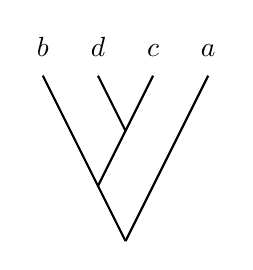
\begin{tikzpicture}[scale=0.7]
    \node[label=above:{$b$}] at (0,0) {};
    \node[label=above:{$d$}] at (1,0) {};
    \node[label=above:{$c$}] at (2,0) {};
    \node[label=above:{$a$}] at (3,0) {};
    \draw[thick] (0,0) to (1.5,-3);
    \draw[thick] (1,0) to (1.5,-1);
    \draw[thick] (2,0) to (1,-2);
    \draw[thick] (3,0) to (1.5,-3);
  \end{tikzpicture}
\] Thanks to the choice of different orderings, the number of
\(T\)-structures on an \(n\)-element set is \(n!\) times the number of
binary trees with \(n\) leaves. Annoyingly, the latter number is
traditionally called the \((n-1)\)st Catalan number, \(C_{n-1}\). So, we
have: \[|T|(x) = \sum_{n=1} C_{n-1} x^n.\]

There's a nice recursive definition of \(T\):

\begin{quote}
``To put a \(T\)-structure on a set, either note that it has one
element, in which case there's just one \(T\)-structure on it, or chop
it into two subsets and put a \(T\)-structure on each one.''
\end{quote}

In other words, any binary tree is either a degenerate tree, with just
one leaf: \[X\] or a pair of binary trees stuck together at the root: \[
  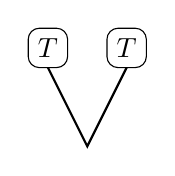
\begin{tikzpicture}
    \draw[rounded corners] (-0.75,1) rectangle (-0.25,1.5);
    \draw[rounded corners] (0.75,1) rectangle (0.25,1.5);
    \node at (-0.5,1.25) {$T$};
    \node at (0.5,1.25) {$T$};
    \draw[thick] (-0.5,1) to (0,0) to (0.5,1);
  \end{tikzpicture}
\] We can write this symbolically as \[T \cong X + T^2\]

Here's why: \(X\) is a structure type called ``being the one-element
set'', \(+\) means ``exclusive or'', and squaring a structure type means
you chop your set in two parts and put that structure on each part. (I
explained these rules more carefully in
\protect\hyperlink{week190}{``Week 190''}.)

Note that we only have an \emph{isomorphism} between structure types
here, not an equation. But if we take the generating function of both
sides we get an actual equation, and the notation is set up to make this
really easy: \[|T| = x + |T|^2\] In \protect\hyperlink{week144}{``Week
144''} I showed how you can solve this using the quadratic equation:
\[|T| = \frac{1-\sqrt{1-4x}}{2}\] and then do a Taylor expansion to get
\[|T| = x + x^2 + 2x^3 + 5x^4 + 14x^5 + 42x^6 + \ldots\]

Lo and behold! The coefficient of \(x^n\) is the number of binary trees
with \(n\) leaves!

There's also another approach where we work directly with the structure
types themselves, instead of taking generating functions. This is harder
because we can't subtract structure types, or divide them by 2, or take
square roots of them --- at least, not without stretching the rules of
this game. All we can do is use the isomorphism \[T \cong X + T^2 \] and
the basic rules of category theory. It's not as efficient, but it's
illuminating. It's also incredibly simple: we just keep sticking in
``\(X + T^2\)'' wherever we see ``\(T\)'' on the right-hand side, over
and over again. Like this: \[
  \begin{aligned}
    T
    &\cong X + T^2
  \\&\cong X + (X + T^2)^2
  \\&\cong X + (X + (X + T^2)^2)^2
  \end{aligned}
\] and so on. You might not think we're getting anywhere, but if you
stop at the \(n\)th stage and expand out what we've got, you'll get the
first \(n\) terms of the Taylor expansion we had before! At least, you
will if you count ``stages'' and ``terms'' correctly.

I won't actually do this, because it's better if you do it yourself.
When you do, you'll see it captures the recursive process of building a
binary tree from lots of smaller binary trees. Each time you see a
``\(T\)'' and replace it with an ``\(X + T^2\)'', you're really taking a
little binary tree: \[
  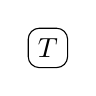
\begin{tikzpicture}
    \draw[rounded corners] (-0.75,1) rectangle (-0.25,1.5);
    \node at (-0.5,1.25) {$T$};
  \end{tikzpicture}
\] and replacing it with either a degenerate tree with just a single
leaf: \[X\] or a pair of binary trees: \[
  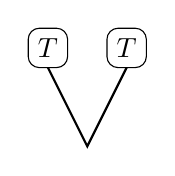
\begin{tikzpicture}
    \draw[rounded corners] (-0.75,1) rectangle (-0.25,1.5);
    \draw[rounded corners] (0.75,1) rectangle (0.25,1.5);
    \node at (-0.5,1.25) {$T$};
    \node at (0.5,1.25) {$T$};
    \draw[thick] (-0.5,1) to (0,0) to (0.5,1);
  \end{tikzpicture}
\] So, each term in the final result actually corresponds to a specific
tree! This is a good example of categorification: when we calculate the
coefficient of \(x^n\) this way, we're not just getting the
\emph{number} of binary planar trees with \(n\) leaves --- we're getting
an actual explicit description of the \emph{set} of such trees.

Now, what happens if we take the generating function \(|T|(x)\) and
evaluate it at \(x = 1\)? On the one hand, we get a divergent series:
\[|T|(1) = 1 + 1 + 2 + 5 + 14 + 42 + \ldots\]

This is the sum of all Catalan numbers --- or in other words, the number
of binary planar trees. On the other hand, we can use the formula
\[|T| = \frac{1-\sqrt{1-4x}}{2}\] to get \[|T| = \frac{1-\sqrt{-3}}{2}\]
It may seem insane to conclude
\[1 + 1 + 2 + 5 + 14 + 42 + \ldots = \frac{1-\sqrt{-3}}{2}\] but Lawvere
noticed that there's a kind of strange sense to it.

The trick is to work not with generating function \(|T|\) but with the
structure type \(T\) itself. Since \(|T|(1)\) is equal to the
\emph{number} of planar binary trees, \(T(1)\) should be naturally
isomorphic to the \emph{set} of planar binary trees. And it is --- it's
obvious, once you think about what it really means.

The number of binary planar trees is not very interesting, but the set
of them is. In particular, if we take the isomorphism
\[T \cong X + T^2\]

and set \(X = 1\), we get an isomorphism \[T(1) \cong 1 + T(1)^2\] which
says

\begin{quote}
``a planar binary tree is either the tree with one leaf or a pair of
planar binary trees.''
\end{quote}

Starting from this, we can derive lots of other isomorphisms involving
the set \(T(1)\), which turn out to be categorified versions of
equations satisfied by the number \[|T|(1) = \frac{1-\sqrt{-3}}{2}\] For
example, this number is a sixth root of unity. While there's no
one-to-one correspondence between \(6\)-tuples of trees and the 1
element set, which would categorify the formula \[|T|(1)^6 = 1\] there
\emph{is} a very nice one-to-correspondence between 7-tuples of trees
and trees, which categorifies the formula \[|T|(1)^7 = |T|(1)\] Of
course the set of binary trees is countably infinite, and so is the set
of 7-tuples of binary trees, so they can be placed in one-to-one
correspondence --- but that's boring. When I say ``very nice'', I mean
something more interesting: starting with the isomorphism
\[T \cong X + T^2\] we get a one-to-one correspondence
\[T(1) \cong 1 + T(1)^2\] which says that any binary planar tree is
either degenerate or a pair of binary planar trees\ldots{} and using
this we can \emph{construct} a one-to-one correspondence
\[T(1)^7 \cong T(1)\]

The construction is remarkably complicated. Even if you do it as
efficiently as possible, I think it takes 18 steps, like this: \[
  \begin{aligned}
    T(1)^7
    \cong&\, T(1)^6 + T(1)^8
  \\\cong&\, \ldots
  \\&\vdots
  \\\cong&\, 1 + T(1) + T(1)^2 + T(1)^4
  \\\cong&\, 1 + T(1) + T(1)^3
  \\\cong&\, 1 + T(1)^2
  \\\cong&\, T(1).
  \end{aligned}
\] I'll let you fill in the missing steps --- it's actually quite fun if
you like puzzles.

If you get stuck, you can find the answer online in a couple of
different places:

\begin{enumerate}
\def\labelenumi{\arabic{enumi})}
\setcounter{enumi}{1}
\item
  Andreas Blass, ``Seven trees in one'', \emph{Jour. Pure Appl. Alg.}
  \textbf{103} (1995), 1--21. Also available at
  \texttt{http://www.math.lsa.umich.edu/\textasciitilde{}ablass/cat.html}
\item
  Marcelo Fiore, ``Isomorphisms of generic recursive polynomial types'',
  to appear in \emph{31st Symposium on Principles of Programming
  Languages (POPL04)}. Also available at
  \texttt{http://www.cl.cam.ac.uk/\textasciitilde{}mpf23/papers/Types/recisos.ps.gz}
\end{enumerate}

Or, take a peek at the ``Addenda'' down below.

Robbie Gates, Marcelo Fiore and Tom Leinster have also proved some very
general theorems about this sort of thing. Gates focused on
``distributive categories'' (categories with with products and
coproducts, the former distributing over the latter), while the work of
Fiore and Leinster applies to more general ``rig categories'':

\begin{enumerate}
\def\labelenumi{\arabic{enumi})}
\setcounter{enumi}{3}
\item
  Robbie Gates, ``On the generic solution to \(P(X) = X\) in
  distributive categories'', \emph{Jour. Pure Appl. Alg.} \textbf{125}
  (1998), 191--212.
\item
  Marcelo Fiore and Tom Leinster, ``Objects of categories as complex
  numbers'', available as
  \href{http://www.arXiv.org/abs/math.CT/0212377}{\texttt{math.CT/0212377}}.
\end{enumerate}

A rig category is basically the most general sort of category in which
we can ``add'' and ``multiply'' as we do in a ring --- but without
negatives, hence the missing letter ``n''. It turns out that whenever we
have an object \(Z\) in a rig category and it's equipped with an
isomorphism \[Z = P(Z)\] where \(P\) is a polynomial with natural number
coefficients, we can associate to it a ``cardinality'' \(|Z|\), namely
any complex solution of the equation \[|Z| = P(|Z|)\] Which solution
should we use? Well, for simplicity let's consider the case where \(P\)
has degree at least 2 and the relevant Galois group acts transitively on
the solutions of this equation, so ``all roots are created equal''. Then
we can pick \emph{any} solution as the cardinality \(|Z|\). Any
polynomial equation with natural number coefficients satisfied by one
solution will be satisfied by \emph{all} solutions, so it won't matter
which one we choose.

Now suppose the cardinality \(|Z|\) satisfies such an equation:
\[Q(|Z|) = R(|Z|)\] where neither \(Q\) nor \(R\) is constant. Then the
results of Fiore and Leinster say we can construct an isomorphism
\[Q(Z) = R(Z)\;\mbox{!}\] In other words, a bunch of equations satisfied
by the object's cardinality automatically come from isomorphisms
involving the object itself.

This explains why the set \(T(1)\) of binary trees acts like it has
cardinality \[|T|(1) = \frac{1-\sqrt{-3}}{2}\] or equally well,
\[|T|(1) = \frac{1+\sqrt{-3}}{2}\] (Since the relevant Galois group
interchanges these two numbers, we can use either one.) More generally,
the set \(T(n)\) consisting of binary trees with \(n\)-colored leaves
acts a lot like the number \(|T|(n)\).

This has gotten me interested in trying to find a nice example of a
``Golden Object'': an object \(G\) in some rig category that's equipped
with an isomorphism \[G^2 = G + 1\] The Golden Object doesn't fit into
Fiore and Leinster's formalism, since this isomorphism is not of the
form \(G = P(G)\) where \(P\) has natural number coefficients. But, it
still seems that such an object deserves to have a ``cardinality'' equal
to the golden number:
\[|G| = \frac{1 + \sqrt{5}}{2} = 1.618033988749894848204586834365\ldots\]

James Propp came up with an interesting idea related to the Golden
Object: consider what happens when we evaluate the generating function
for binary trees at \(-1\). On the one hand we get an alternating sum of
Catalan numbers: \[|T|(-1) = -1 + 1 - 2 + 5 - 14 + 42 + \ldots\] On the
other hand, we can use the formula \[|T| = \frac{1 - \sqrt{1 - 4x}}{2}\]
to get \[|T|(-1) = \frac{1 - \sqrt{5}}{2}\] which is \(-1\) divided by
the golden number. Of course, it's possible we should use the other sign
of the square root, and get \[|T|(-1) = {1 + \sqrt{5}}{2}\] which is
just the golden number! Galois theory says these two roots are created
equal. Either way, we get a bizarre and fascinating formula:
\[- 1 + 1 - 2 + 5 - 14 + 42 + \ldots = \frac{1\pm\sqrt{5}}{2}\] Can we
fit this into some clear and rigorous framework, or is it just nuts?
We'd like some generalization of cardinality for which ``the set of
binary trees with \(-1\)-colored leaves'' has cardinality equal to the
golden number.

James Propp suggested one avenue. A while back, Steve Schanuel made an
incredibly provocative observation: if we treat ``Euler measure'' as a
generalization of cardinality, it makes sense to treat the real line as
a ``space of cardinality \(-1\)'':

\begin{enumerate}
\def\labelenumi{\arabic{enumi})}
\setcounter{enumi}{5}
\item
  Stephen H. Schanuel, ``What is the length of a potato?: an
  introduction to geometric measure theory'', in \emph{Categories in
  Continuum Physics}, Springer Lecture Notes in Mathematics
  \textbf{1174}, Springer, Berlin, 1986, pp.~118--126.
\item
  Stephen H. Schanuel, ``Negative sets have Euler characteristic and
  dimension'', Lecture Notes in Mathematics \textbf{1488}, Springer
  Verlag, Berlin, 1991, pp.~379--385.
\end{enumerate}

James Propp has developed this idea in a couple of fascinating papers:

\begin{enumerate}
\def\labelenumi{\arabic{enumi})}
\setcounter{enumi}{7}
\item
  James Propp, ``Euler measure as generalized cardinality'', available
  as
  \href{http://arxiv.org/abs/math/0203289}{\texttt{arXiv:math/0203289}}.
\item
  James Propp, ``Exponentiation and Euler measure'', available as
  \href{http://arxiv.org/abs/math/0204009}{\texttt{arXiv:math/0204009}}.
\end{enumerate}

Using this idea, it seems reasonable to consider the space of binary
trees with leaves labelled by real numbers as a rigorous version of
``the set of binary trees with \(-1\)-colored leaves''. So, we just need
to figure out what generalization of Euler characteristic gives this
space an Euler characteristic equal to the golden number. It would be
great if we could make this space into a Golden Object in some rig
category, but that may be asking too much.

Whew! There's obviously a lot of work left to be done here. Here's
something easier: a riddle. What's this sequence?

\begin{quote}
un, dos, tres, quatre, cinc, sis, set, vuit, nou, deu,\ldots{}
\end{quote}

The answer is at the end of this article.

Now I'd like to mention some important papers on \(n\)-categories. You
may think I'd lost interest in this topic, because I've been talking
about other things. But it's not true!

Most importantly, Tom Leinster has come out with a big book on
\(n\)-categories and operads:

\begin{enumerate}
\def\labelenumi{\arabic{enumi})}
\setcounter{enumi}{9}
\tightlist
\item
  Tom Leinster, \emph{Higher Operads, Higher Categories}, Cambridge U.
  Press, Cambridge, 2003. Also available as
  \href{http://arxiv.org/abs/math.CT/0305049}{\texttt{arXiv:math.CT/0305049}}.
\end{enumerate}

As you'll note, he managed to talk the press into letting him keep his
book freely available online! We should all do this. Nobody will ever
make much cash writing esoteric scientific tomes --- it takes so long,
you could earn more per hour digging ditches. The only \emph{financial}
benefit of writing such a book is that people will read it, think you're
smart, and want to hire you, promote you, or invite you to give talks in
cool places. So, maximize your chances of having people read your books
by keeping them free online! People will still buy the paper version if
it's any good\ldots.

And indeed, Leinster's book has many virtues besides being free. He
gracefully leads the reader from the very basics of category theory
straight to the current battle front of weak \(n\)-categories,
emphasizing throughout how operads automatically take care of the
otherwise mind-numbing thicket of ``coherence laws'' that inevitably
infest the subject. He doesn't take well-established notions like
``monoidal category'' and ``bicategory'' for granted --- instead, he
dives in, takes their definitions apart, and compares alternatives to
see what makes these concepts tick. It's this sort of careful thinking
that we desperately need if we're ever going to reach the dream of a
clear and powerful theory of higher-dimensional algebra. He does a
similar careful analysis of ``operads'' and ``multicategories'' before
presenting a generalized theory of operads that's powerful enough to
support various different approaches to weak \(n\)-categories. And then
he describes and compares some of these different approaches!

In short: if you want to learn more about operads and \(n\)-categories,
this is \emph{the} book to read.

Leinster doesn't say too much about what \(n\)-categories are good for,
except for a nice clear introduction entitled ``Motivation for
Topologists'', where he sketches their relevance to homology theory,
homotopy theory, and cobordism theory. But this is understandable, since
a thorough treatment of their applications would vastly expand an
already hefty 380-page book, and diffuse its focus. It would also steal
sales from \emph{my} forthcoming book on higher-dimensional algebra ---
which would be really bad, since I plan to retire on the fortune I'll
make from this.

Secondly, Michael Batanin has worked out a beautiful extension of his
ideas on \(n\)-categories which sheds new light on their applications to
homotopy theory:

\begin{enumerate}
\def\labelenumi{\arabic{enumi})}
\setcounter{enumi}{10}
\item
  Michael A. Batanin, ``The Eckmann-Hilton argument, higher operads and
  \(E_n\) spaces'', available as
  \href{http://arxiv.org/abs/math.CT/0207281}{\texttt{arXiv:math.CT/0207281}}.

  Michael A. Batanin, ``The combinatorics of iterated loop spaces'',
  available as
  \href{http://arxiv.org/abs/math.CT/0301221}{\texttt{arXiv:math.CT/0301221}}.
\end{enumerate}

Getting a manageable combinatorial understanding of the space of loops
in the spaces of loops in the space of loops\ldots{} in some space has
always been part of the dream of higher-dimensional algebra. These
``\(k\)-fold loop spaces'' or have been important in homotopy theory
since the 1970s --- see the end of \protect\hyperlink{week199}{``Week
199''} for a little bit about them. People know that \(k\)-fold loop
spaces have \(k\) different products that commute up to homotopy in a
certain way that can be summarized by saying they are algebras of the
\(E_k\) operad, also called the ``little \(k\)-cubes operad''. However,
their wealth of structure is still a bit mind-boggling. James Dolan and
I made some conjectures about their relation to \(k\)-tuply monoidal
categories in our paper ``Categorification'' (see
\protect\hyperlink{week121}{``Week 121''}), and now Batanin is making
this more precise using his approach to \(n\)-categories --- which is
one of the ones described in Leinster's book.

There's also been a lot of work applying higher-dimensional algebra to
topological quantum field theory --- that's what got me interested in
\(n\)-categories in the first place, but a lot has happened since then.
For a highly readable introduction to the subject, with tons of great
pictures, try:

\begin{enumerate}
\def\labelenumi{\arabic{enumi})}
\setcounter{enumi}{11}
\tightlist
\item
  Joachim Kock, \emph{Frobenius Algebras and 2D Topological Quantum
  Field Theories}, Cambridge U. Press, Cambridge, 2003.
\end{enumerate}

This is mainly about 2d TQFTs, where the concept of ``Frobenius
algebra'' reigns supreme, and everything is very easy to visualize.

When we go up to \(3\)-dimensional spacetime life gets harder, but also
more interesting. This book isn't so easy, but it's packed with
beautiful math and wonderfully drawn pictures:

\begin{enumerate}
\def\labelenumi{\arabic{enumi})}
\setcounter{enumi}{12}
\tightlist
\item
  Thomas Kerler and Volodymyr L. Lyubashenko, \emph{Non-Semisimple
  Topological Quantum Field Theories for \(3\)-Manifolds with Corners},
  Lecture Notes in Mathematics \textbf{1765}, Springer, Berlin, 2001.
\end{enumerate}

The idea is that if we can extend the definition of a quantum field
theory to spacetimes that have not just boundaries but \emph{corners},
we can try to build up the theory for arbitrary spacetimes from its
behavior on simple building blocks --- since it's easier to chop
manifolds up into a few basic shapes if we let those shapes have
corners. However, it takes higher-dimensional algebra to describe all
the ways we can stick together manifolds with corners! Here Kerler and
Lyubashenko make \(3\)-dimensional manifolds going between
\(2\)-manifolds with boundary into a ``double category''\ldots{} and
make a bunch of famous 3d TQFTs into ``double functors''.

Closely related is this paper by Kerler:

\begin{enumerate}
\def\labelenumi{\arabic{enumi})}
\setcounter{enumi}{13}
\tightlist
\item
  Thomas Kerler, ``Towards an algebraic characterization of
  3-dimensional cobordisms'', \emph{Contemp. Math.} \textbf{318} (2003)
  141--173. Also available as
  \href{http://arxiv.org/abs/math/0106253}{\texttt{arXiv:math/0106253}}.
\end{enumerate}

It relates the category whose objects are \(2\)-manifolds with a circle
as boundary, and whose morphisms are \(3\)-manifolds with corners going
between these, to a braided monoidal category ``freely generated by a
Hopf algebra object''. (I'm leaving out some fine print here, but
probably putting in more than most people want!) It comes close to
showing these categories are the same, but suggests that they're not
quite --- so the perfect connection between topology and higher
categories remains elusive in this important example.

Answer to the riddle: these are the Catalan numbers --- i.e., the
natural numbers as written in Catalan. This riddle was taken from the
second volume of Stanley's book on enumerative combinatorics (see
\protect\hyperlink{week144}{``Week 144''}).

\begin{center}\rule{0.5\linewidth}{0.5pt}\end{center}

\textbf{Addenda:} Long after this issue was written, we had a discussion
on the \(n\)-Category Café about the ``seven trees in one'' problem. Let
\(B\) be the set of binary planar trees --- the set I was calling
\(T(1)\) above. Starting from the isomorphism \[B \cong B^2 + 1\] we
want to construct an isomorphism \[B \cong B^7\] Here is the proof in
Marcelo Fiore's paper:
\[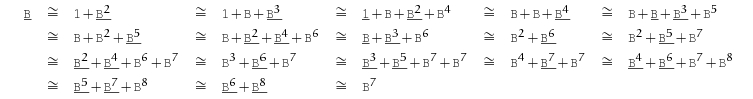
\includegraphics[max width=\linewidth]{../images/seven_trees_in_one_fiore.jpg}\]
At each step he either replaces \(B^n\) by \(B^{n-1} + B^{n+1}\), or the
reverse. The underlined portion shows where this will be done. Over at
the \emph{n}-Café, Stuart Presnell made a beautiful picture of this
proof:
\[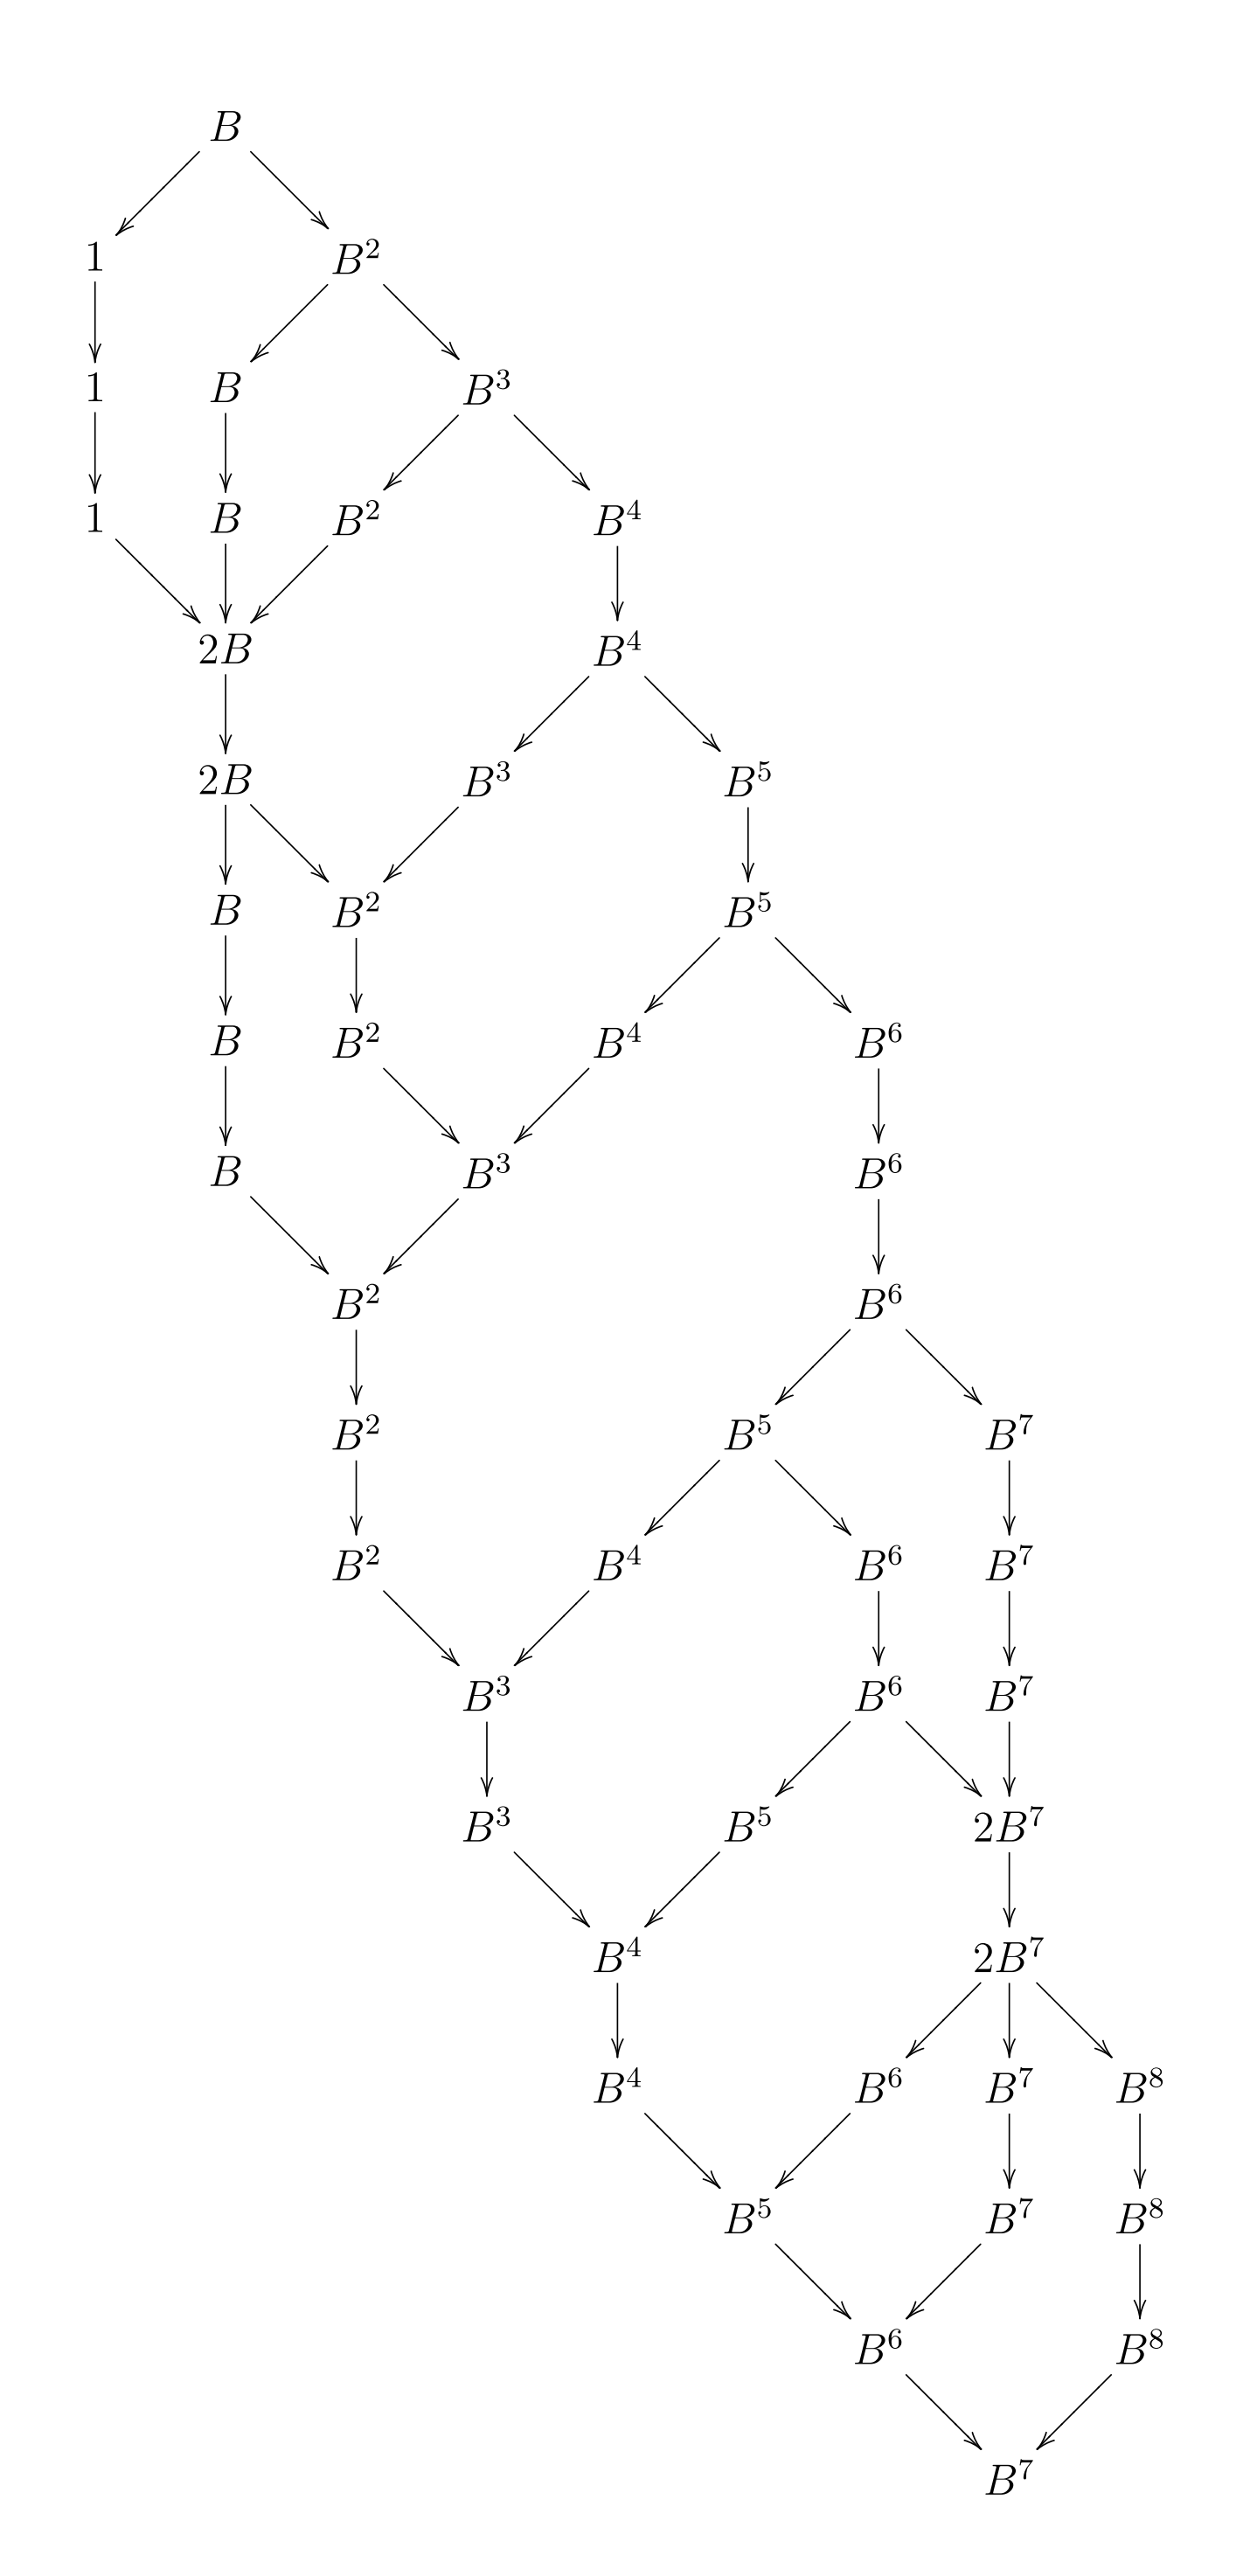
\includegraphics[max width=\linewidth]{../images/seven_trees_in_one_presnell_fiore.png}\]
He also made a picture of another proof, which is on page 29 of Pierre
Ageron's book Logiques, Ensembles, Catgories: Le Point de Vue
Constructif:
\[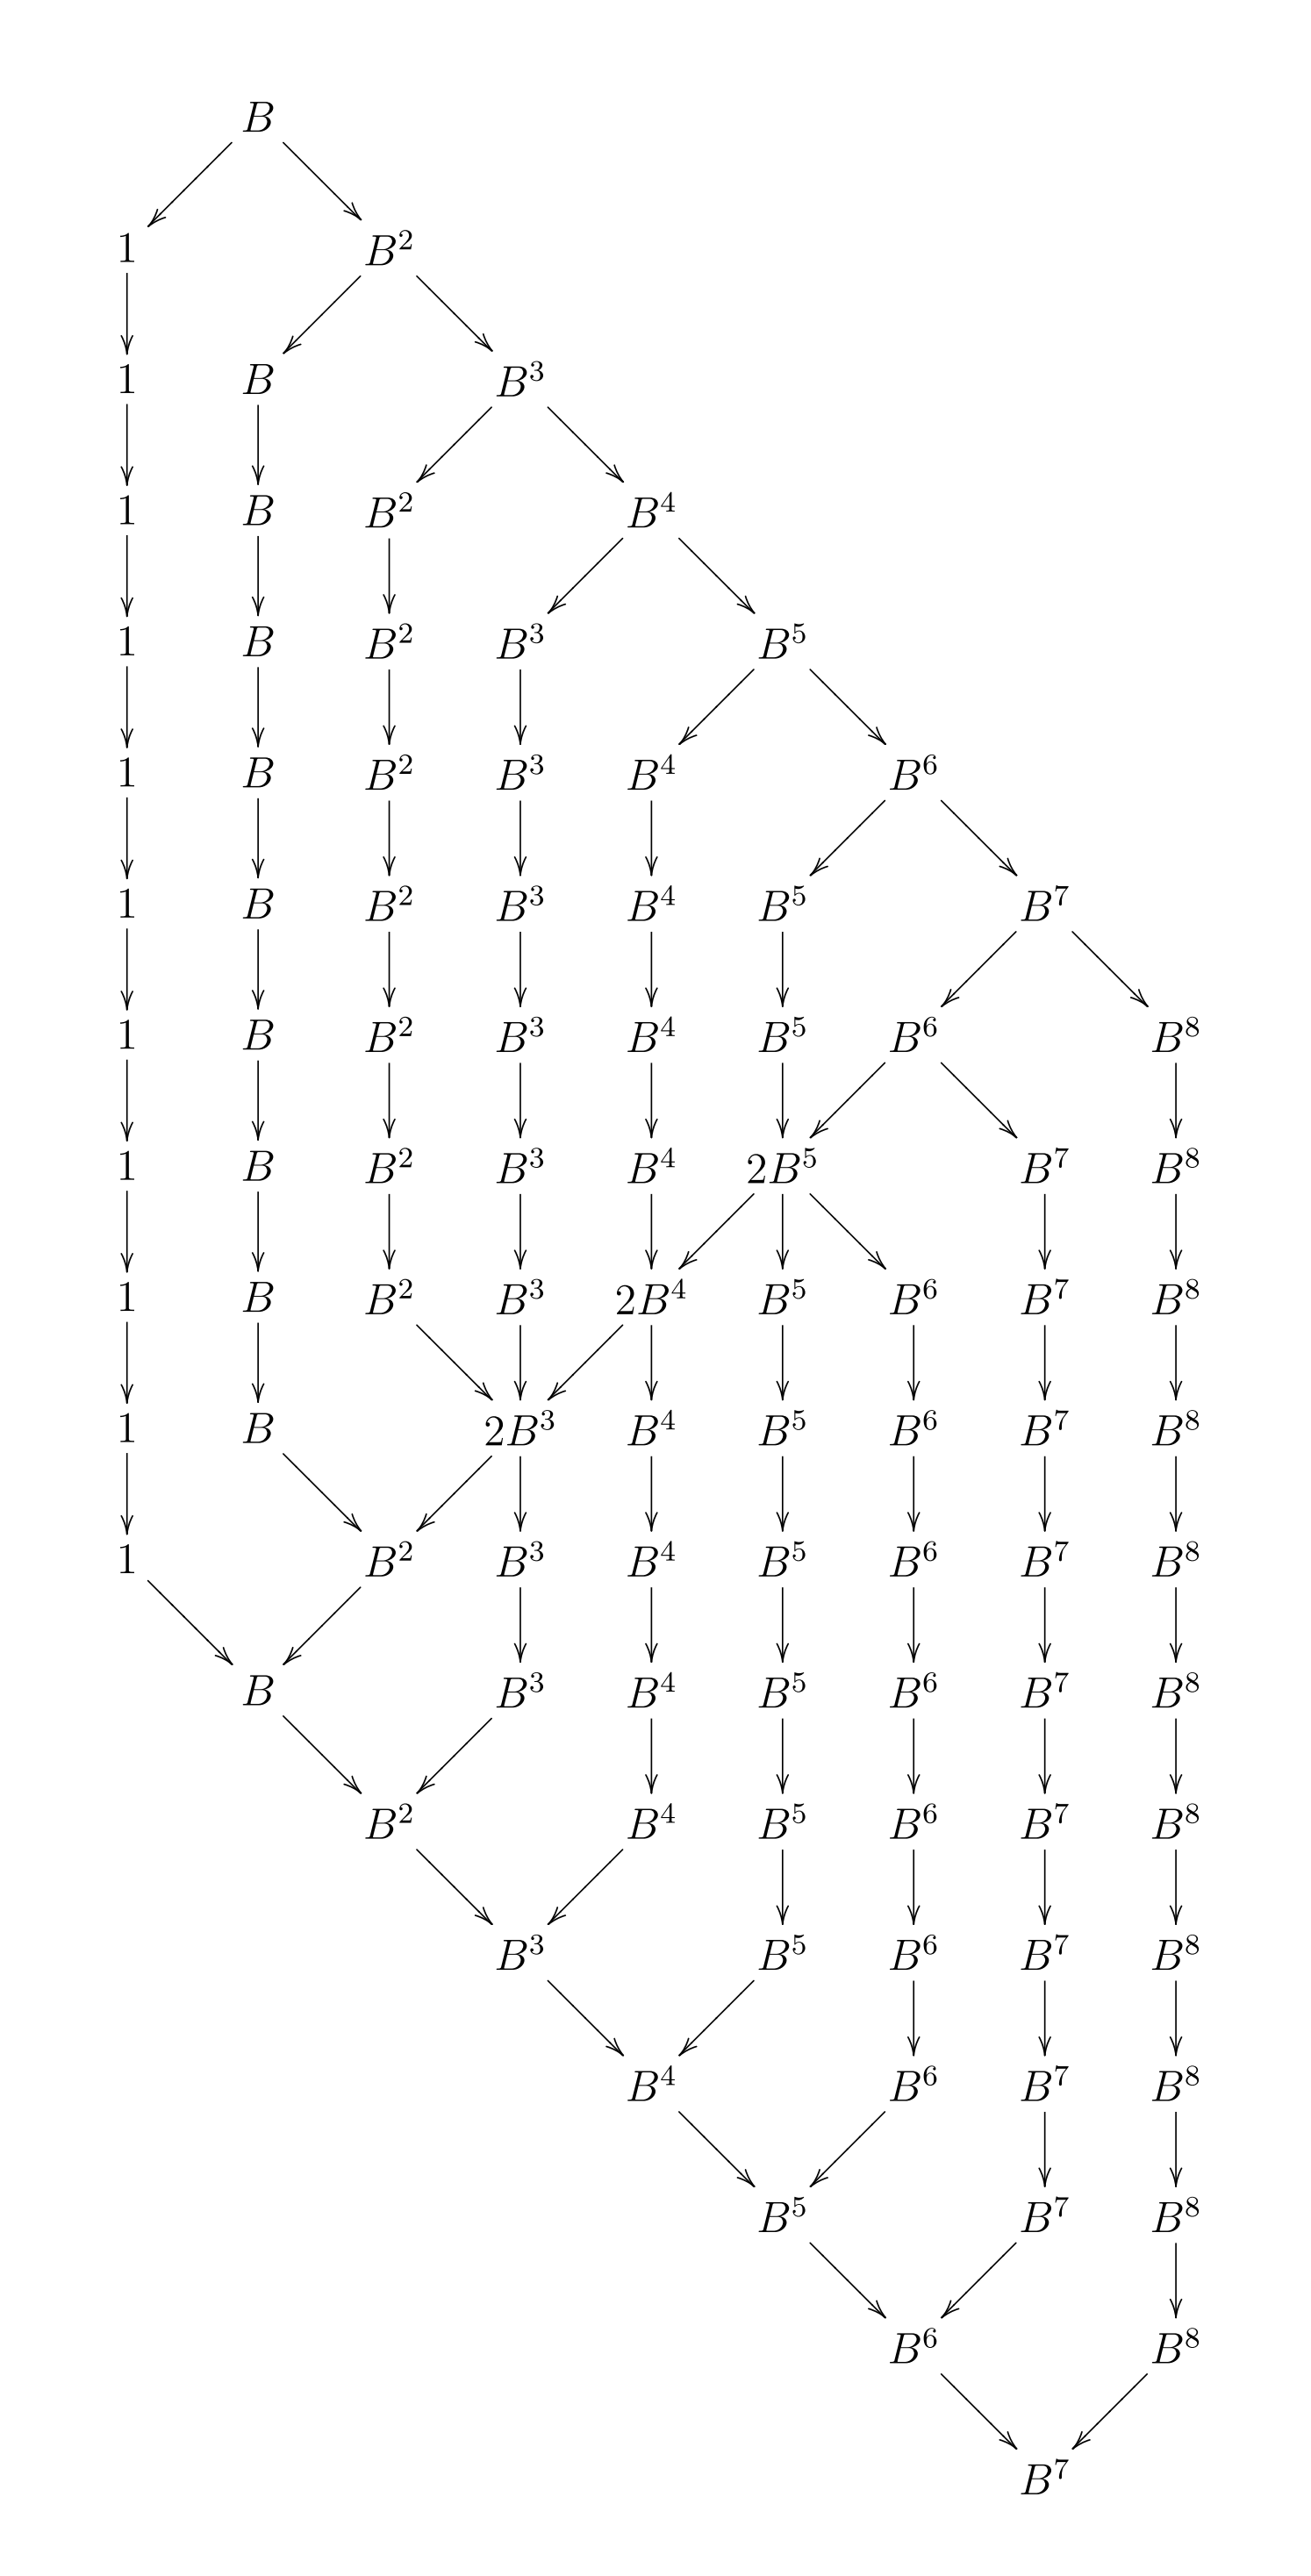
\includegraphics[max width=\linewidth]{../images/seven_trees_in_one_presnell_bell.png}\]
You can watch a \emph{movie} of a proof here:

\begin{enumerate}
\def\labelenumi{\arabic{enumi})}
\setcounter{enumi}{14}
\tightlist
\item
  Dan Piponi," Arboreal isomorphisms from nuclear pennies", \emph{A
  Neighborhood of Infinity}, September 30, 2007. Available at
  \texttt{http://blog.sigfpe.com/2007/09/arboreal-isomorphisms-from-nuclear.html}.
\end{enumerate}

It was in the ensuing discussion on this blog that George Bell came up
with his more efficient proof. For a bit more discussion, see:

\begin{enumerate}
\def\labelenumi{\arabic{enumi})}
\setcounter{enumi}{15}
\tightlist
\item
  John Baez, `Searching for a video proof of ``seven trees in one''\,',
  \(n\)-Category Café, July 16, 2009. Available at
  \texttt{http://golem.ph.utexas.edu/category/2009/07/searching\_for\_a\_video\_proof\_of.html}.
\end{enumerate}

Now, on to some older addenda!

My pal Squark pointed out that if we try to compute the generating
function for binary trees by making an initial guess for \(|T|(x)\), say
\(t\), and repeatedly improving this guess via \[t \mapsto x + t^2\] the
guess will converge to the right answer if \(t\) is small --- but the
process will fail miserably, with \(t\) approaching \(\infty\), if and
only if the complex number \(x\) lies outside the Mandelbrot set!

After an earlier version of this Week appeared on the category theory
mailing list, Steve Schanuel posted some corrections. I've tried to
correct the text above as much as possible without making it too
technical --- for example, by citing the important work of Robbie Gates,
and distinguishing more clearly between his work on distributive
categories and the paper by Fiore and Leinster, which applies to rig
categories. I tend to talk about 3 different sorts of ring-like
categories in This Week's Finds:

\begin{itemize}
\item
  Rig categories. A \textbf{rig category} is one equipped with a
  symmetric monoidal structure called \(+\) and a monoidal structure
  called \(\otimes\), with all the usual rig axioms holding up to
  natural isomorphism, and these isomorphisms satisfying a set of
  coherence laws worked out by Laplaza and Kelly:

  \begin{enumerate}
  \def\labelenumi{\arabic{enumi})}
  \setcounter{enumi}{16}
  \item
    M. Laplaza, ``Coherence for distributivity'', Lecture Notes in
    Mathematics \textbf{281}, Springer Verlag, Berlin, 1972, pp.~29--72.
  \item
    G. Kelly, ``Coherence theorems for lax algebras and distributive
    laws'', Lecture Notes in Mathematics \textbf{420}, Springer Verlag,
    Berlin, 1974, pp.~281--375.
  \end{enumerate}

  (These authors spoke of ``ring categories'', but the term ``rig
  category'' is more appropriate since, as in a rig, there need be no
  additive inverses.)
\item
  \(2\)-Rigs. A \textbf{2-rig} is a symmetric monoidal cocomplete
  category where the monoidal structure, which we call \(\otimes\),
  distributes over the colimits, which we think of as a generalized form
  of addition. For more on rigs, \(2\)-rigs and structure types see
  \href{week191.html}{week191}. In a \(2\)-rig, distributivity is just a
  property of the monoidal structure, rather than a structure, as it is
  in a rig category. However, by choosing a particular coproduct for
  each pair of objects, and a particular initial object, we can promote
  any \(2\)-rig to a rig category. To get an example of a rig category
  that's not a \(2\)-rig, just take any rig and think of it as a
  discrete category (a category with only identity morphisms). Another
  example would be the category of finite-dimensional vector spaces,
  since this only has finite colimits. (Of course, we could make up some
  sort of ``finitary \(2\)-rig'' that only had finite colimits, but the
  profusion of terminology is already annoying.)
\item
  Distributive categories. A \textbf{distributive category} is a
  category with finite products and coproducts, the products
  distributing over the coproducts. Here again, distributivity is just a
  property. But, by choosing specified products and coproducts for every
  pair of objects, and choosing terminal and initial objects, we can
  promote any distributive category into a rig category. A good example
  of a \(2\)-rig that is not a distributive category is the category
  \(\mathsf{Vect}\), with direct sum and tensor product as \(+\) and
  \(\otimes\). Another example is the discrete category on a rig.
\end{itemize}

By not distinguishing these, the original version of
\protect\hyperlink{week202}{``Week 202''} made it sound as if Fiore and
Leinster had simply redone Gates' work on distributive categories. I
hope this is a bit clearer now. Schanuel's remarks are still worth
reading for their description of what Gates actually did:

\begin{quote}
Dear colleagues,

For those who read the most recent long discursion of John Baez, a few
of the errors in the section on distributive categories merit
correction:

\begin{enumerate}
\def\labelenumi{(\arabic{enumi})}
\item
  J. B. suggests that Blass published what Lawvere had already worked
  out. In fact, Lawvere (partly to counteract some incorrect uses of
  infinite series in analyses of `data types' in computer science) had
  worked out the algebra of the rig presented by one generator \$ \$and
  one relation \(X=1+X^2\), roughly by the method in (3) below, and
  conjectured that this rig could be realized as the isomorphism classes
  in a distributive (even extensive) category, which conjecture Blass
  then proved (and a bit more) in ``Seven Trees\ldots{}''.
\item
  The generalization of Blass's theorem to one generator ond one
  polynomial relation of the `fixed-point' form \(X=p(X)\), where \(p\)
  is a polynomial with natural number coefficients and nonzero constant
  term is not, as J. B. seems to suggest, due to Fiore and Leinster; it
  was part of the prize-winning doctoral thesis of Robbie Gates, who
  (using a calculus of fractions) described explicitly the free
  distributive category on one object \(X\) together with an isomorphism
  from \(p(X)\) to \(X\), proving that this category is extensive and
  that its rig of isomorphism classes satisfies no further relations,
  i.e.~is the rig \(R\) presented by one generator and the one relation
  above.
\item
  If \(p\) is as in (2) and of degree at least 2, the algebra of the rig
  \(R\) is made by J. B. to seem mysterious. It is more easily
  understood in the way the \(X=2^X+1\) case was treated in my
  ``Negative Sets\ldots{}'' paper; just show that the Euler and
  dimension homomorphisms, tensoring with \(\mathbb{Z}\) and with
  \(\mathsf{2}\) (the rig true/false) respectively, are jointly
  injective. In this case the dimension rig has only three elements,
  which explains why the Euler characteristic captures almost, but not
  quite, everything.
\end{enumerate}

Greetings to all,\\
Steve Schanuel
\end{quote}

\begin{center}\rule{0.5\linewidth}{0.5pt}\end{center}

\begin{quote}
\emph{A traveller who refuses to pass over a bridge until he personally
tests the soundness of every part of it is not likely to go far;
something must be risked, even in mathematics.}

--- Horace Lamb
\end{quote}



\hypertarget{week203}{%
\section{February 28, 2004}\label{week203}}

Last week I posed this puzzle: to find a ``Golden Object''.

A couple days ago I got a wonderful solution from Robin Houston, a
computer science grad student at the University of Manchester. So, I
want to say a bit more about the golden number, then describe his
solution, and then describe how he found it.

Supposedly the Greeks thought the most beautiful rectangle was one such
that when you chop a square off one end, you're left with a rectangle of
the same shape. If your original rectangle was \(1\) unit across and
\(G\) units long, after you chop a \(1\)-by-\(1\) square off the end
you're left with a rectangle that's \(G-1\) units across and \(1\) unit
long: \[
  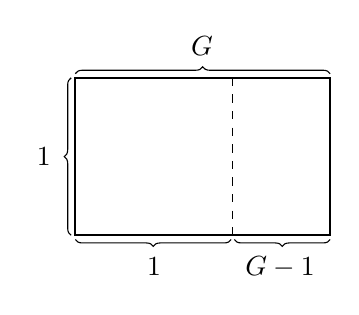
\begin{tikzpicture}[scale=2]
    \draw[thick] (0,0) rectangle (1.618,1);
    \draw[dashed] (1,1) to (1,0);
    \draw[decoration={brace,raise=1.5,mirror},decorate] (0,0) to (0.99,0);
    \draw[decoration={brace,raise=1.5,mirror},decorate] (1.01,0) to (1.618,0);
    \draw[decoration={brace,raise=1.5},decorate] (0,0) to (0,1);
    \draw[decoration={brace,raise=1.5},decorate] (0,1) to (1.618,1);
    \node at (0.5,-0.2) {$1$};
    \node at (1.3,-0.2) {$G-1$};
    \node at (-0.2,0.5) {$1$};
    \node at (0.805,1.2) {$G$};
  \end{tikzpicture}
\] So, to make the proportions of the little rectangle the same as those
of the big one, you want

\begin{quote}
``1 is to G as G-1 is to 1''
\end{quote}

or in other words: \[\frac{1}{G} = G - 1 \] or after a little algebra,
\[G^2 = G + 1\] so that
\[G = \frac{1+\sqrt{5}}{2} = 1.618033988749894848204586834365\ldots\]
while \[\frac1G = 1.618033988749894848204586834365\ldots\] and
\[G^2 = 2.618033988749894848204586834365\ldots\] (At this point I
usually tell my undergraduates that the pattern continues like this,
with \(G^3 = 3.618\ldots\) and so on --- just to see if they'll believe
anything I say.)

These days, the number \(G\) is called the Golden Number, the Golden
Ratio, or the Golden Section. It's often denoted by the Greek letter
\(\Phi\), after the Greek sculptor Phidias. Phidias helped design the
Parthenon - and supposedly packed it full of golden rectangles, to make
it as beautiful as possible.

The golden number is a great favorite among amateur mathematicians,
because it has a flashy sort of charm. You can find it all over the
place if you look hard enough --- and if you look too hard, you'll find
it even in places where it's not. It's the ratio of the diagonal to the
side of a regular pentagon! If you like the number 5, you'll be glad to
know that \[G = \sqrt{\frac{5+\sqrt{5}}{5-\sqrt{5}}}\] If you don't,
maybe you'd prefer this:
\[G = \exp\left(\operatorname{arcsinh}\left(\frac12\right)\right)\] My
favorite formulas for the golden number are
\[G = \sqrt{1 + \sqrt{1 + \sqrt{1 + \sqrt{1 + \sqrt{1 + \sqrt{1 + \ldots}}}}}}\]
and the continued fraction:
\[G = 1 + \frac{1}{1 + \frac{1}{1 + \frac{1}{1 + \frac{1}{1 + }}}}\]
These follow from the equations \(G^2 = G + 1\) and \(G = 1 + 1/G\),
respectively. If you chop off the continued fraction for \(G\) at any
point, you'll see that \(G\) is also the limit of the ratios of
successive Fibonacci numbers. See \protect\hyperlink{week190}{``Week
190''} for a very different proof of this fact.

However, don't be fooled! The charm of the golden number tends to
attract kooks and the gullible --- hence the term ``fool's gold''. You
have to be careful about anything you read about this number. In
particular, if you think ancient Greeks ran around in togas
philosophizing about the ``golden ratio'' and calling it ``\(\Phi\)'',
you're wrong. This number was named \(\Phi\) after Phidias only in 1914,
in a book called \emph{The Curves of Life} by the artist Theodore Cook.
And, it was Cook who first started calling \(1.618\ldots\) the golden
ratio. Before him, \(\ldots0.618\) was called the golden ratio! Cook
dubbed this number ``\(\varphi\)'', the lower-case baby brother of
\(\Phi\).

In fact, the whole ``golden'' terminology can only be traced back to
1826, when it showed up in a footnote to a book by one Martin Ohm,
brother of Georg Ohm, the guy with the law about resistors. Before then,
a lot of people called \(1/G\) the ``Divine Proportion''. And the guy
who started \emph{that} was Luca Pacioli, a pal of Leonardo da Vinci who
translated Euclid's \emph{Elements}. In 1509, Pacioli published a
3-volume text entitled \emph{Divina Proportione}, advertising the
virtues of this number. Some people think da Vinci used the divine
proportion in the composition of his paintings. If so, perhaps he got
the idea from Pacioli.

Maybe Pacioli is to blame for the modern fascination with the golden
ratio; it seems hard to trace it back to Greece. These days you can buy
books and magazines about ``Elliot Wave Theory'', a method for making
money on the stock market using patterns related to the golden number.
Or, if you're more spiritually inclined, you can go to workshops on
``Sacred Geometry'' featuring talks about the healing powers of the
golden ratio. But Greek texts seem remarkably quiet about this number.

The first recorded hint of it is
\href{http://aleph0.clarku.edu/~djoyce/java/elements/bookII/propII11.html}{Proposition
11 in Book II} of Euclid's \emph{Elements}. It also shows up elsewhere
in Euclid, especially
\href{http://aleph0.clarku.edu/~djoyce/java/elements/bookVI/propVI30.html}{Proposition
30 of Book VI}, where the task is ``to cut a given finite straight line
in extreme and mean ratio'', meaning a ratio \(A:B\) such that \[
  \begin{gathered}
    A:B :: (A+B):A
  \\\mbox{i.e. "$A$ is to $B$ as $A+B$ is to $A$"}
  \end{gathered}
\] This is later used in
\href{http://aleph0.clarku.edu/~djoyce/java/elements/bookXIII/propXIII17.html}{Proposition
17 of Book XIII} to construct the pentagonal face of a regular
dodecahedron.

Of course, Euclid wasn't the first to do all these things; he just wrote
them up in a nice textbook. By now it's impossible to tell who
discovered the golden ratio and just what the Greeks thought about it.
For a sane and detailed look at the history of the golden ratio, try
this:

\begin{enumerate}
\def\labelenumi{\arabic{enumi})}
\tightlist
\item
  J. J. O'Connor and E. F. Robertson, ``The Golden Ratio'',
  \texttt{http://www-gap.dcs.st-and.ac.uk/\textasciitilde{}history/HistTopics/Golden\_ratio.html}
\end{enumerate}

While I'm at it, I should point out that Theodore Cook's book
introducing the notation ``\(\Phi\)'' is still in print:

\begin{enumerate}
\def\labelenumi{\arabic{enumi})}
\setcounter{enumi}{1}
\tightlist
\item
  Theodore A. Cook, \emph{The Curves of Life: Being an Account of Spiral
  Formations and Their Application to Growth in Nature, to Science, and
  to Art: with Special Reference to the Manuscripts of Leonardo da
  Vinci}, Dover Publications, New York, 1979.
\end{enumerate}

If you want to see what Euclid said about the golden ratio, you can also
pick up a cheap copy of the Elements from Dover --- but it's probably
quicker to go online. There are a number of good places to find Euclid's
Elements online these days.

Topologists know David Joyce as the inventor of the ``quandle'' --- an
algebraic structure that captures most of the information in a knot. Now
he's writing a high-tech edition of Euclid, complete with Java applets:

\begin{enumerate}
\def\labelenumi{\arabic{enumi})}
\setcounter{enumi}{2}
\tightlist
\item
  David E. Joyce's edition of Euclid's Elements,
  \texttt{http://aleph0.clarku.edu/\textasciitilde{}djoyce/java/elements/toc.html}
\end{enumerate}

Joyce is carrying on a noble tradition: back in 1847, Oliver Byrne did a
wonderful edition of Euclid complete with lots of beautiful color
pictures and even some pop-up models. You can see this online at the
Digital Mathematics Archive:

\begin{enumerate}
\def\labelenumi{\arabic{enumi})}
\setcounter{enumi}{3}
\tightlist
\item
  Oliver Byrne's edition of Euclid's Elements, online at the Digital
  Mathematics Archive,
  \texttt{http://www.sunsite.ubc.ca/DigitalMathArchive/}
\end{enumerate}

The most famous scholarly English translation of Euclid was done by Sir
Thomas Heath in 1908. You can find it together with an edition in Greek
and a nearly infinite supply of other classical texts at the Perseus
Digital Library:

\begin{enumerate}
\def\labelenumi{\arabic{enumi})}
\setcounter{enumi}{4}
\tightlist
\item
  Thomas L. Heath's edition of Euclid's Elements, online at The Perseus
  Digital Library, \texttt{http://www.perseus.tufts.edu/}
\end{enumerate}

But I'm digressing! My main point was that while
\(G = (1 + \sqrt{5})/2\) is a neat number, it's a lot easier to find
nuts raving about it on the net than to find truly interesting
mathematics associated with it --- or even interesting references to it
in Greek mathematics! The cynic might conclude that the charm of this
number is purely superficial. However, that would be premature.

First of all, there's a certain sense in which \(G\) is ``the most
irrational number''. To get the best rational approximations to a number
you use its continued fraction expansion. For \(G\), this converges as
slowly as possible, since it's made of all 1's:
\[G = 1 + \frac{1}{1 + \frac{1}{1 + \frac{1}{1 + \frac{1}{1 + }}}}\] We
can make this more precise. For any number \(x\) there's a constant
\(c(x)\) that says how hard it is to approximate \(x\) by rational
numbers, given by
\[\liminf_{q\to\infty}\left\vert x-\frac{p}{q}\right\vert = \frac{c(x)}{q^2}\]
where \(q\) ranges over integers, and \(p\) is an integer chosen to
minimize \(|x - p/q|\). This constant is as big as possible when \(x\)
is the golden ratio!

It'd be ironic if the famously ``rational'' Greeks, who according to
legend even drowned the guy who proved \(\sqrt{2}\) was irrational,
chose the most irrational number as the proportions of their most
beautiful rectangle! But, it wouldn't be a coincidence. Their obsession
with ratios and proportions led them to ponder the situation where
\(A:B::(A+B):A\), and this proportion instantly implies that \(A\) and
\(B\) are incommensurable, since if you assume \(A\) and \(B\) are
integers and try to find their greatest common divisor using Euclid's
algorithm, you get stuck in an infinite loop. Euclid even mentions this
idea in
\href{http://aleph0.clarku.edu/~djoyce/java/elements/bookX/propX2.html}{Proposition
2 of Book X}:

\begin{quote}
If, when the less of two unequal magnitudes is continually subtracted in
turn from the greater that which is left never measures the one before
it, then the two magnitudes are incommensurable.
\end{quote}

He doesn't explicitly come out and apply it to what we now call the
golden ratio --- but how could he not have made the connection? For more
info on the Greek use of continued fractions and the Euclidean
algorithm, check out the chapter on ``antihyphairetic ratio theory'' in
this book:

\begin{enumerate}
\def\labelenumi{\arabic{enumi})}
\setcounter{enumi}{5}
\tightlist
\item
  D. H. Fowler, \emph{The Mathematics of Plato's Academy: A New
  Reconstruction}, Oxford U. Press, Oxford, 1987.
\end{enumerate}

Anyway, it's actually important in physics that the golden number is so
poorly approximated by rationals. This fact shows up in the Kolmogorov-
Arnold-Moser theorem, or ``KAM theorem'', which deals with small
perturbations of completely integrable Hamiltonian systems. Crudely
speaking, these are classical mechanics problems that have as many
conserved quantities as possible. These are the ones that tend to show
up in textbooks, like the harmonic oscillator and the gravitational
2-body problem. The reason is that you can solve such problems if you
can do a bunch of integrals --- hence the term ``completely
integrable''.

The cool thing about a completely integrable system is that time
evolution carries states of the system along paths that wrap around
tori. Suppose it takes \(n\) numbers to describe the position of your
system. Then it also takes \(n\) numbers to describe its momentum, so
the space of states is \(2n\)-dimensional. But if the system has n
different conserved quantities --- that's basically the maximum allowed
--- the space of states will be foliated by \(n\)-dimensional tori. Any
state that starts on one of these tori will stay on it forever! It will
march round and round, tracing out a kind of spiral path that may or may
not ever get back to where it started.

Things are pretty simple when \(n = 1\), since a \(1\)-dimensional torus
is a circle, so the state \emph{has} to loop around to where it started.
For example, when you have a pendulum swinging back and forth, its
position and momentum trace out a loop as time passes.

When n is bigger, things get trickier. For example, when you have n
pendulums swinging back and forth, their motion is periodic if the
ratios of their frequencies are rational numbers.

This is how it works for any completely integrable system. For any
torus, there's an \(n\)-tuple of numbers describing the frequency with
which paths on this torus wind around in each of the \(n\) directions.
If the ratios of these frequencies are all rational, paths on this torus
trace out periodic orbits. Otherwise, they don't!

KAM theory says what happens when you perturb such a system a little. It
won't usually be completely integrable anymore. Interestingly, the tori
with rational frequency ratios tend to fall apart due to resonance
effects. Instead of periodic orbits, we get chaotic motions instead. But
the ``irrational'' tori are more stable. And, the ``more irrational''
the frequency ratios for a torus are, the bigger a perturbation it takes
to disrupt it! Thus, the most stable tori tend to have frequency ratios
involving the golden number. As we increase the perturbation, the last
torus to die is called a ``golden torus''.

You can actually \emph{watch} tori breaking into chaotic dust if you
check out the applet illustrating the ``standard map'' on this website:

\begin{enumerate}
\def\labelenumi{\arabic{enumi})}
\setcounter{enumi}{6}
\tightlist
\item
  Takashi Kanamaru and J. Michael T. Thompson, ``Introduction to Chaos
  and Nonlinear Dynamics'', standard map applet,
  \texttt{http://brain.cc.kogakuin.ac.jp/\textasciitilde{}kanamaru/Chaos/e/Standard/}
\end{enumerate}

The ``standard map'' is a certain dynamical system that's good for
illustrating this effect. You won't actually see 2d tori, just 1d
cross-sections of them --- but it's pretty fun. For more details, try
this:

\begin{enumerate}
\def\labelenumi{\arabic{enumi})}
\setcounter{enumi}{7}
\tightlist
\item
  M. Tabor, \emph{Chaos and Integrability in Nonlinear Dynamics: An
  Introduction}, Wiley, New York, 1989.
\end{enumerate}

In short, the golden number is the best frequency ratio for avoiding
resonance!

Some audiophiles even say this means the best shaped room for listening
to music is one with proportions \(1:G:G^2\). I leave it to you to find
the flaw in this claim. For more dubious claims, check out the ad for
expensive speaker cables at the end of this article.

KAM theory is definitely cool, but we shouldn't rest content with this
when skeptics ask if the golden number is all it's cracked up to be. I
figure it's part of our job as mathematicians to keep on discovering
mind-blowing facts about the golden number. A small part, but part: we
shouldn't give up the field to amateurs!

Penrose has done his share. His ``Penrose tiles'' take crucial advantage
of the self-similarity embodied by the golden number to create
nonperiodic tilings of the plane. This helped spawn a nice little
industry, the study of ``quasicrystals'' with \(5\)-fold symmetry.
Here's a good introduction for mathematicians:

\begin{enumerate}
\def\labelenumi{\arabic{enumi})}
\setcounter{enumi}{8}
\tightlist
\item
  Andre Katz, ``A short introduction to quasicrystallography'', in
  \emph{From Number Theory to Physics}, eds.~M. Waldschmit et al,
  Springer, Berlin, 1992, pp.~496--537.
\end{enumerate}

By the way, this same book has some nice stuff on the role of the golden
number in KAM theory and the theory of iterated maps from the circle to
itself:

\begin{enumerate}
\def\labelenumi{\arabic{enumi})}
\setcounter{enumi}{9}
\item
  Predrag Cvitanovic, ``Circle maps: irrationally winding'', in
  \emph{From Number Theory to Physics}, eds.~M. Waldschmit et al,
  Springer, Berlin, 1992, pp.~631--658.
\item
  Jean-Christophe Yoccoz, ``Introduction to small divisors problems'',
  in \emph{From Number Theory to Physics}, eds.~M. Waldschmit et al,
  Springer, Berlin, 1992, pp.~659--679.
\end{enumerate}

Conway and Sloane are also pulling their weight. Starting from the
relation between the golden ratio, the isosahedron, and the
\(4\)-dimensional big brother of the icosahedron (the ``600-cell''),
they've described how to construct the coolest lattices in 8 and 24
dimensions using ``icosians'' --- which are certain quaternions built
using the golden ratio. I discussed this circle of ideas in
\protect\hyperlink{week20}{``Week 20''},
\protect\hyperlink{week59}{``Week 59''} and
\protect\hyperlink{week155}{``Week 155''}.

But if you want some really scary formulas involving the golden ratio,
Ramanujan is the one to go to. Check these out:
\[\frac{1}{1 + \frac{\exp(-2\pi)}{1 + \frac{\exp(-4\pi)}{1 + \frac{\exp(-6\pi)}{1 + \ldots}}}} = \exp\left(\frac{2\pi}{5}\right)\left(\sqrt{G\sqrt{5}}-5\right)\]
and
\[1 + \frac{\exp(-2\pi\sqrt{5})}{1 + \frac{\exp(-4\pi\sqrt{5})}{1 + \frac{\exp(-6\pi\sqrt{5})}{1 + \ldots}}} = \exp\left(\frac{2\pi}{5}\right)\left(\frac{\sqrt{5}}{1+(5^\frac34(G-1)^\frac52-1)^\frac15}-G\right)\]
These are special cases of a monstrosity called the Rogers-Ramanujan
continued fraction, which is a kind of ``\(q\)-deformation'' of the
continued fraction for the golden ratio. For details, start here:

\begin{enumerate}
\def\labelenumi{\arabic{enumi})}
\setcounter{enumi}{11}
\tightlist
\item
  Eric W. Weisstein, ``Rogers-Ramanujan Continued Fraction'',
  \texttt{http://mathworld.wolfram.com/Rogers-RamanujanContinuedFraction.html}
\end{enumerate}

It's these two formulas, and one other like it, that led Hardy to write
the famous lines:

\begin{quote}
A single look at them is enough to show that they could only be written
down by a mathematician of the highest class. They must be true because,
if they were not true, no one would have had the imagination to invent
them.
\end{quote}

For more by Hardy on these continued fractions, see section 1 and
section 6.17 of his book:

\begin{enumerate}
\def\labelenumi{\arabic{enumi})}
\setcounter{enumi}{12}
\tightlist
\item
  G. H. Hardy, \emph{Ramanujan: Twelve Lectures on Subjects Suggested by
  His Life and Work}, Chelsea Publishing Co., New York, 1959.
\end{enumerate}

The golden number also shows up in the theory of quantum groups. I
talked about this in \protect\hyperlink{week22}{``Week 22''} so I won't
explain it again here. But, I can't resist mentioning that Freedman,
Larsen and Wang have subsequently shown that a certain topological
quantum field theory called Chern-Simons theory, built using the quantum
group \(\mathrm{SU}_q(2)\), can serve as a universal quantum computer
when the parameter \(q\) is a fifth root of unity. And, this is exactly
the case where the spin-\(1/2\) representation of \(\mathrm{SU}_q(2)\)
has quantum dimension equal to the golden number!

\begin{enumerate}
\def\labelenumi{\arabic{enumi})}
\setcounter{enumi}{13}
\tightlist
\item
  Michael Freedman, Michael Larsen, Zhenghan Wang, ``A modular functor
  which is universal for quantum computation'', available at
  \href{http://www.arXiv.org/quant-ph/0001108}{\texttt{quant-ph/0001108}}.
\end{enumerate}

But don't get the wrong idea: it's not that some magic feature of the
golden number is required to build a universal quantum computer! It's
just that the 5 seems to be the \emph{smallest} number \(n\) such that
\(\mathrm{SU}_q(2)\) Chern-Simons theory is computationally universal
when \(q\) is an \(n\)th root of \(1\).

That's pretty much everything I know about the golden number. So now,
what about this ``Golden Object'' puzzle?

Basically, the problem was to find an object that acts like the golden
number. The golden number has \(G^2 = G + 1\), so we want to find a
object \(G\) equipped with a nice isomorphism between \(G^2\) and
\(G + 1\).

If \(G\) is just a set, this means we want a nice one-to-one
correspondence between pairs of elements of \(G\), and elements of \(G\)
together with one other thing. It doesn't matter what that other thing
is, so let's call it ``\(@\)''.

(You may be wondering about the word ``nice''. The point is, the problem
is too easy if we don't demand that the solution be nice in some way ---
some way that I don't feel like making precise.)

Here's Robin Houston's answer:

Define a ``bit'' to be either \(0\) or \(1\). Define a ``golden tree''
to be a (planar) binary tree with leaves labelled by \(0\), \(1\), or
\(*\), where every node has at most one bit-child. For example: \[
  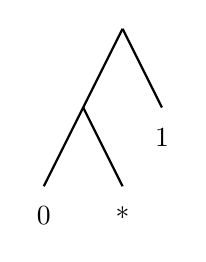
\begin{tikzpicture}
    \draw[thick] (0,0) to (-1,-2) node[label=below:{$0$}]{};
    \draw[thick] (0,0) to (0.5,-1) node[label=below:{$1$}]{};
    \draw[thick] (-0.5,-1) to (0,-2) node[label=below:{$*$}]{};
  \end{tikzpicture}
\] is a golden tree, but \[
  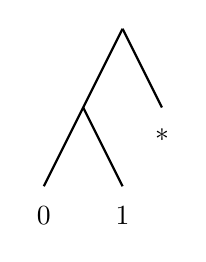
\begin{tikzpicture}
    \draw[thick] (0,0) to (-1,-2) node[label=below:{$0$}]{};
    \draw[thick] (0,0) to (0.5,-1) node[label=below:{$*$}]{};
    \draw[thick] (-0.5,-1) to (0,-2) node[label=below:{$1$}]{};
  \end{tikzpicture}
\] is not. Let \(G\) be the set of golden trees. We define an
isomorphism \[f\colon G^2 \to G + \{@\}\] as follows. First we define
\(f(X, Y)\) when both \(X\) and \(Y\) are golden trees with just one
node, this node being labelled by a bit. We can identify such a tree
with a bit, and doing this we set \[
  \begin{aligned}
    f(0, 0) &= 0
  \\f(0, 1) &= 1
  \\f(1, 0) &= *
  \\f(1, 1) &= @
  \end{aligned}
\] In the remaining case, where the golden trees X and Y are not just
bits, we set \[
  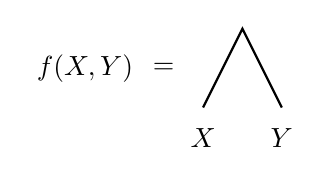
\begin{tikzpicture}
    \node at (0,0) {$f(X,Y)$};
    \node at (1,0) {$=$};
    \draw[thick] (1.5,-0.5) node[label=below:{$X$}]{} to (2,0.5) to (2.5,-0.5) node[label=below:{$Y$}]{};
  \end{tikzpicture}
\] There are different ways to show this function \(f\) is a one-to-one
correspondence, but the best way is to see how Houston came up with this
answer! He didn't just pull it out of a hat; he tackled the problem
systematically, and that's why his solution counts as ``nice''.

It's easy to find a set \(S\) equipped with an isomorphism \[S = P(S)\]
where \(P\) is some polynomial with natural number coefficients. You
just use the fixed-point principle described in
\protect\hyperlink{week108}{``Week 108''}. Namely, you start with the
empty set, keep hitting it with \(P\) forever, and take a kind of limit.
This is how I built the set of binary trees last week, as a solution of
\(T = T^2 + 1\).

The problem is that the isomorphism we seek now: \[G^2 = G + 1 \tag{1}\]
is not of this form. So, what Houston does is to make a substitution:
\[G = H + 2\] Given this, we'd get (1) if we had
\[H^2 + 4H + 4 = H + 3 \tag{2}\] and we'd get (2) if we had
\[H^2 + 4H + 1 = H \tag{3}\] which is of the desired form.

We can rewrite (3) as \[H = 1 + H^2 + 2H + H2\] and in English this says
"an element of \(H\) is either a *, or a pair consisting of two guys
that are either bits or elements of \(H\) --- but not both bits". So, a
guy in \(H\) is a golden tree! But, if it has just one node, that node
can only be labelled by a \(*\), not a \(0\) or \(1\). This means there
are precisely 2 golden trees not in \(H\). So, \(G = H + 2\) is the set
of all golden trees, and our calculation above gives an isomorphism
\(G^2 = G + 1\).

Voila!

Note that to derive (3) from (1) we need to subtract, which in general
is not allowed in this game. Here we are subtracting constants, and
Houston says that's allowed by the ``Garsia-Milne involution theorem''.
I don't know this theorem, so I'll make a note to myself to learn it.
But luckily, we don't really need it here: we only need to derive (1)
from (3), and that involves addition, so it's fine.

Part of what makes Houston's solution ``nice'' is that it suggests a
general method for turning polynomial equations into recursive
definitions of the form \(S = P(S)\). Another nice thing is that his
trick delivers a structure type \(G(X)\) that reduces to \(G\) when
\(X = 1\). To get this, first use the fixed-point method to construct a
structure type \(H(X)\) with an isomorphism
\[H(X) = (H(X) + X)^2 + 2H(X)\] Then, define \[G(X) = H(X) + X + 1\] and
note that this gives \[G(X)^2 = G(X) + X\] which reduces to G\^{}2 = G +
1 when X = 1.

As if this weren't enough, Houston also gave another solution to the
puzzle. He showed that James Propp's proposed Golden Object, described
last week, really is a Golden Object! Maybe Propp already knew this, but
I sure didn't.

The idea of the proof is pretty general. Suppose we're in some category
that's a ``\(2\)-rig'' in the sense of
\protect\hyperlink{week191}{``Week 191''}. And, suppose we've got an
object X equipped with an isomorphism \[X = 1 + 2X \tag{4}\] so that
\(X\) acts like ``\(-1\)''. For example, following Schanuel and Propp,
we can take the category of ``\(\sigma\)-polytopes'' and let \(X\) be
the open interval: then isomorphism (4) says
\[(0,1) = (0,1/2) + \{1/2\} + (1/2,1)\] Or, following Houston, we can
take the category of sets and let \(X\) be the set of finite
bit-strings. Then (4) says ``a finite bit-string is either the empty
bit-string, or a bit followed by a finite bit-string''. The relation
between these two examples is puzzling to me --- if anyone understands
it, let me know! But anyway, either one works.

Now let \(G\) be the object of ``binary trees with \(X\)-labelled
leaves'': \[G = X + X^2 + 2X^3 + 5X^4 + 14X^5 + 42X^6 + \ldots\] where
the coefficients are Catalan numbers. Let's show that \(G\) is a Golden
Object. To do this, we'll use (4) and this isomorphism:
\[G = G^2 + X \tag{5}\] which says ``a binary tree with \(X\)-labelled
leaves is a pair of such trees, or a degenerate tree with just one
\(X\)-labelled node''. The formula for \(G\) involving Catalan numbers
is really just the fixed-point solution to this!

Here is Houston's fiendishly clever argument. Suppose \(Z\) is any type
equipped with an isomorphism \[Z = Z' + X\] for some \(Z'\). Then \[
  \begin{aligned}
    Z + X + 1
    &= Z' + 2X + 1
  \\&= X' + X
  \\&= Z
  \end{aligned}
\] This applies to \(Z = G^2\), since
\[G^2 = (X + G^2)^2 = (2X + 1 + G^2)^2\] has a \(X\) term in it when you
multiply it out, so it's of the form \(Z' + X\). Therefore we have an
isomorphism \[G^2 = G^2 + X + 1\] But we also have an isomorphism
\(G + 1 = G^2 + X + 1\) by (5). Composing these, we get our isomorphism
\[G^2 = G + 1.\] Golden! I'll stop here.

\begin{center}\rule{0.5\linewidth}{0.5pt}\end{center}

\textbf{Addendum:} The computer scientist Sebastiano Vigna pointed out
this paper:

\begin{enumerate}
\def\labelenumi{\arabic{enumi})}
\setcounter{enumi}{14}
\tightlist
\item
  Paolo Boldi, Massimo Santini, and Sebastiano Vigna, ``Measuring with
  jugs, or: what if mathematicians were asked to defuse bombs?'',
  \emph{Theoret. Comput. Sci.} \textbf{2} (2002). Also available at
  \texttt{http://vigna.dsi.unimi.it/papers.php}
\end{enumerate}

which shows that if you want to approximately measure an arbitrary
amount of water using only two jugs, it's best if they have capacity
\(1\) and \(G\). This paper cites a a charming result by Swierczkowski
which picks up where a famous theorem due to Dedekind leaves off.
Dedekind showed that if \(x\) is any irrational number, the numbers
\(nx \mod 1\) are uniformly distributed in the interval \([0,1]\). But
if \(x = 1/G\), these numbers have an especially nice property: each new
point in the sequence \((nx \mod 1)\) lands in one of the \emph{longest}
intervals not containing a previous point! And, it chops this interval
in a golden way.

Stephen Schanuel said some things about
\protect\hyperlink{week203}{``Week 203''} on the category theory mailing
list, so I'll include his post here along with various replies,
concluding with my own.

\begin{verbatim}
From:   Stephen Schanuel 
Subject: categories: mystification and categorification
Date:   Thu, 4 Mar 2004 00:44:46 -0500  

    I was unable to understand John Baez' golden object problem, nor his
description of the solutions.  He refuses to tell us what 'nice' means,
but let me at least propose that to be 'tolerable' a solution must be an
object in a category, and John doesn't tell us what category is involved
in either of the solutions; at least I couldn't find a specification of
the objects, nor the maps, so I found the descriptions 'intolerable', in
the technical sense defined above.  He is very generous, allowing one to
use a category with both plus and times as extra monoidal structures.
(Does anyone know an example of interest in which the plus is not
coproduct?)  This freedom is unnecessary; a little algebra plus Robbie
Gates' theorem provides a solution G to G^2=G+1 which satisfies no
additional equations, in an extensive category (with coproduct as plus,
cartesian product as times).
    Briefly, here it is.  A primitive fifth root of unity z is a root of
the polynomial 1+X+X^2+X^3+X^4, hence satisfies 1+z+z^2+z^3+z^4+z=z,
which is of the 'fixed point' form p(z)=z with p in N[X] and p(0) not
0. Gates' theorem then says that the free distributive category
containing an object Z and an isomorphism from p(Z) to Z is extensive,
and its Burnside rig B (of isomorphism classes of objects) is, as one
would hope, N[X]/(p(X)=X); that is, Z satisfies no unexpected
equations. Since the degree of p is greater than 1, an easy general
theorem tells us (from the joint injectivity of the Euler and dimension
homomorphisms) that two polynomials agree at the object Z if and only if
either they are the same polynomial or both are non-constant and they
agree at the number z.Now the 'algebra':  the golden number is 1+z+z^4.
So G=1+Z+Z^4 satisfies G^2=G+1, as desired. It satisfies no
unexpected equations, because the relation X^2=X+1 reduces any
polynomial in N[X] to a linear polynomial, and these reduced forms have
distinct Euler characteristics, i.e. differ at z. Thus the homomorphism
from N[X]/(X^2=X+1) to B (sending X to G) is injective, and that's all
I wanted.
    Since in the category of sets, any nasty old infinite set satisfies
the golden equation and many others, I have taken the liberty of
interpreting  'nice' to mean at least 'satisfying no unexpected
equations'. One could ask for more; the construction above has produced
a distributive, but not extensive, category whose Burnside rig is
N[X]/(X^2=X+1), the full subcategory with objects polynomials in G.
(If it were extensive, it would be closed under taking summands, but
every object in the larger category is a summand of G.) I don't know
whether there is an extensive category with N[X]/(X^2=X+1) as its full
Burnside rig; perhaps one or both of the examples John mentioned would
do, if I knew what they were.
    While I'm airing my confusions, can anyone tell me what
'categorification' means? I don't know any such process; the simplest
exanple, 'categorifying' natural numbers to get finite sets, seems to me
rather 'remembering the finite sets and maps which gave rise to natural
numbers by the abstraction of passing to isomorphism classes'.
   Finally, a note to John: While you're trying to give your audience
some feeling for the virtues of $n$-categories, couldn't you give them a
little help with n=1, by being a little more precise about objects and
maps?
   Greetings to all, and thanks for your patience while I got this stuff
off my chest,
   Steve Schanuel





From:    David Yetter 
Subject: categories: Re: mystification and categorification
Date:    Fri, 5 Mar 2004 10:55:26 -0600 

Categorification is a bit like quantization:  it isn't a construction so much
as a desideratum for a relationship between one thing and another (in the
case of categorification an $(n+1)$-categorical structure and an $n$-categorical
structure; in the case of quantization a quantum mechanical system and
a classical mechanical system).

Categorification wants to find a higher-dimensional categorical structure
corresponding to a lower-dimensional one by weakening equations to
natural isomorphisms and imposing new, sensible, coherence conditions.
In general, for the original purpose for which it was proposed--constructions
of TQFT's and models of quantum gravity--one wants the highest categorical
level to have a linear structure (hence Baez wanting tensor product
and a sum it distributes over, rather than cartesian product and coproduct).
Specific lower-dimensional categories with structure are 'categorified' by
finding a higher-dimensional category with the new structure which 'lies over'
the lower dimensional one in the way an additive monoidal category lies
over its Grothendieck rig.

For instance any (k-linear) monoidal category with monoid of isomorphism
classes M is a categorification of M, and more generally (k-linear) monoidal
categories are a categorification of monoids.

A simple example shows why it is not a construction:  commutative monoids
(as rather special categories with one object) admit two different
categorifications:  symmetric monoidal categories and braided monoidal
categories (each regarded as a kind of bicategory with one object).
There is a good argument for regarding braided monoidal categories
as the 'correct' categorification:  the Eckmann-Hilton theorem ('a group
in GROUPS is an abelian group'  or, really as the proof shows, 'a monoid
in MONOIDS is a commutative monoid') 'categorifies' to: A monoidal category
in MONCAT is a braided monoidal category.





From:    Vaughan Pratt 
Subject: categories: Re: mystification and categorification
Date:    Fri, 05 Mar 2004 22:49:56 -0800    

>While I'm airing my confusions, can anyone tell me what
>'categorification' means? I don't know any such process; the simplest
>exanple, 'categorifying' natural numbers to get finite sets, seems to me
>rather 'remembering the finite sets and maps which gave rise to natural
>numbers by the abstraction of passing to isomorphism classes'.

A fair question.  I attended John's Coimbra lectures on this stuff in 1999
but a lot of it leaked out afterwards.  If I had to guess I'd say he was
categorifying the free monoid on one generator to make it a monoidal category,
but then how did the monoid end up as coproduct and the generator as the
final object?  One suspects some free association there---John, how do
you make that connection?

With regard to categorification in general, sets seem to play a central
role in at least one development of category theory.  The homobjects of
"ordinary" categories are homsets.  (In that sense I guess "ordinary" must
entail "locally small.")  $2$-categories are what you get if instead you let
them be homcats, suitably elaborated.

Going in the other direction, if you take homsets to be vacuous, not
in the sense that they are empty but rather that they are all the same,
then you get sets.  One more step in that direction makes everything look
the same, which may have something to do with the Maharishi Yogi hiring
category theorists for the math dept. of his university in Fairfield, Iowa.
(When I spoke last with the MY's "Minister of World Health," an MD who like
Ross Street was a classmate of mine but eight years earlier starting in 1957,
the entire conversation seemed to be largely a skirting of the minefield
of the sameness of everything, which may subconsciously have been behind my
obscure reply to Peter Freyd's posting a while back about unique existence
going back to Descartes, where I tried to one-up him by claiming it went
much further back.)

Categorification isn't the only way to get to $2$-categories, which can be
understood instead in terms of the interchange law as a two-dimensional
associativity principle.  However John has got a lot of mileage out of
the categorification approach, which one can't begrudge in an era where
mileage and minutes are as integral to a balanced life as one's checkbook.
(Q: How many minutes in a month?  A: Depends on your plan.)

>Since in the category of sets, any nasty old infinite set satisfies
>the golden equation and many others, I have taken the liberty of
>interpreting 'nice' to mean at least 'satisfying no unexpected
>equations'.

Quite right.  I would add to this "and satisfying the expected equations."
The "nasty sets" of which Steve speaks fail to satisy such expected
equations as 2^2X ~ X.  (The power set of a set is a Boolean algebra,
for heaven's sake.  Why on earth forget that structure prior to taking the
second exponentiation?  \mathsf{Set} theorists seem to think that they can simply
forget structure without paying for it, but in the real world it costs
kT/2 joules per element of X to forget that structure.  If set theorists
aren't willing to pay real-world prices in their modeling, why should we
taxpayers pay them real-world salaries?  Large cardinals are a figment of
their overactive imaginations, and the solution to consistency concerns is
not to go there.)

Vaughan Pratt





From: Tom Leinster 
Subject: Re: categories: mystification and categorification
Date: 07 Mar 2004 20:50:39 +0000

Steve Schanuel wrote:
> a category with both plus and times as extra monoidal structures.
> (Does anyone know an example of interest in which the plus is not
> coproduct?) 

Here are two examples that I've come across previously of rig categories
in which the plus is not coproduct:

(i) the category of finite sets and bijections, with + and x inherited
from the category of sets;

(ii) discrete rig categories, which are of course the same thing as
rigs.

> This freedom is unnecessary; a little algebra plus Robbie
> Gates' theorem provides a solution G to  G^2=G+1 which satisfies no
> additional equations, in an extensive category (with coproduct as plus,
> cartesian product as times).

If you do allow yourself the freedom to use any rig category then an
even simpler solution exists, also satisfying no additional equations:
just take the rig freely generated by an element G satisfying G^2 = G +
1 and regard it as a discrete rig category.

>     Since in the category of sets, any nasty old infinite set satisfies
> the golden equation and many others, I have taken the liberty of
> interpreting  'nice' to mean at least 'satisfying no unexpected
> equations'.

I'd interpret "nice" differently.  (Apart from anything else, the
trivial example in my previous paragraph would otherwise make the golden
object problem uninteresting.)  "Nice" as I understand it is not a
precise term - at least, I don't know how to make it precise.  Maybe I
can explain my interpretation by analogy with the equation T = 1 + T^2. 
A nice solution T would be the set of finite, binary, planar trees
together with the usual isomorphism T -~-> 1 + T^2; a nasty solution
would be a random infinite set T with a random isomorphism to 1 + T^2. 
(Both these solutions are in the rig category \mathsf{Set} with its standard +
and x.)  I regard the first solution as nice because I can see some
combinatorial content to it (and maybe, at the back of my mind, because
it has a constructive feel), and the second as nasty because I can't. 
I'm not certain what I think of the solution given by the set of
not-necessarily-finite binary planar trees (nice?), or by the set of
binary planar trees of cardinality at most aleph_5 (probably nasty).

Maybe the finding of a "nice" solution is similar in spirit to the
finding of a "concrete interpretation" of a combinatorial identity.  As
an extremely simple example, consider the identity saying that each
entry in Pascal's triangle is the sum of the two above it,

   (n+1 choose r) = (n choose r-1) + (n choose r).

This is a doddle to prove, but all the same you'd be missing something
if you didn't know the standard "concrete interpretation": choosing r
objects out of n+1 objects amounts to EITHER choosing the first one and
then choosing r-1 of the remaining n OR ... .  Even if the challenge of
finding a "nice solution" or "concrete interpretation" isn't made
precise, I think there is a shared sense of what would count as an
answer, and finding an answer is in general not straightforward.

Best wishes,
Tom





From: John Baez
Subject: golden objects
Date: Sun, 7 Mar 2004 12:50:29 -0800 (PST)

Dear Categorists -

Sorry to take a while to respond.  People at UCR have been unable to
receive posts on the category theory mailing list, due to problems with
our internet connection.  

I'd asked for some nice examples of an object G in a rig category
equipped with an isomorphism from G^2 to G + 1.  Steve Schanuel replied:

>I was unable to understand John Baez' golden object problem, nor his
>description of the solutions.  He refuses to tell us what 'nice' means, [...]

The problem was deliberately open-ended, but you seem to have 
understood it perfectly, since you've given a nice solution, 
including a precise specification of what you consider "nice".  

Let me repeat the two solutions given by Robin Houston:

1) The first solution works in any rig category having an object H 
equipped with an isomorphism to H^2 + 4H + 1.  The solution is to take

G = H + 2.

I described how Houston uses the isomorphism H \to H^2 + 4H + 1 to 
construct an isomorphism G^2 \to G + 1.  

What's nice about this is that it reduces a problem that's not 
obviously of fixed-point form to one that is.

2) Houston's second solution works in any monoidal cocomplete category, 
tensor product distributing over colimits, that contains an object X 
equipped with an isomorphism to 2X + 1.  The solution is to let G be 
the object of "binary planar rooted trees with X-labelled leaves", i.e.

G = X + X^2 + 2X^3 + 5X^4 + 14X^5 + 42X^6 + ...

where the coefficients are Catalan numbers.  He uses the obvious 
isomorphism G \to G^2 + X to construct an isomorphism G^2 \to G + 1.

What's nice about this is that it shows Propp's originally proposed
golden object really is one: just take the category of $\sigma$-polytopes 
with its cartesian product, and let X be the open interval!  And,
it makes precise the sense in which the alternating sum of Catalan
numbers equals the golden ratio.

Steve writes:

>I don't know whether there is an extensive category with N[X]/(X^2=X+1) 
>as its full Burnside rig; perhaps one or both of the examples John 
>mentioned would do, if I knew what they were.

I think example 1) does the job if we take the free distributive
category on an object H equipped with an isomorphism to H^2 + 4H + 1.
Right?

Steve also writes:

>He is very generous, allowing one to use a category with both plus 
>and times as extra monoidal structures.  (Does anyone know an example 
>of interest in which the plus is not coproduct?)  This freedom is 
>unnecessary [...]

It's unnecessary, but handy: I think there's also an golden object in 
the rig category of reps of quantum \mathrm{SU}(2) at a suitable value of q.  
Here the tensor product is not cartesian.  

In the lingo of quantum group theory, this object has "quantum dimension"
equal to the golden number.  It's interesting how such nonintegral but 
algebraic "dimensions" show up naturally in quantum group theory, 
just as nonintegral but algebraic "cardinalities" show up in the theory 
of distributive categories.  

I don't know any golden objects in rig categories where the plus is
not coproduct, and I agree that such rig categories arise less often
than those where times is not product.  But, if you use the obvious 
way of making the groupoid of finite sets into a rig category, + isn't 
coproduct, nor is x product.  

> While I'm airing my confusions, can anyone tell me what
> 'categorification' means? I don't know any such process; the simplest
> exanple, 'categorifying' natural numbers to get finite sets, seems to me
> rather 'remembering the finite sets and maps which gave rise to natural
> numbers by the abstraction of passing to isomorphism classes'.

You're right: categorification is not a systematic process!  
I explained this idea back in week121, and also in my paper
"Categorification", at http://www.arXiv.org/abs/math.QA/9802029.  
Here's what I said:

 If one studies categorification one soon discovers an amazing fact: many
 deep-sounding results in mathematics are just categorifications of facts
 we learned in high school!  There is a good reason for this.  All along,
 we have been unwittingly `decategorifying' mathematics by pretending
 that categories are just sets.  We `decategorify' a category by
 forgetting about the morphisms and pretending that isomorphic objects
 are equal.  We are left with a mere set: the set of isomorphism classes
 of objects. 

 To understand this, the following parable may be useful.  Long ago, when
 shepherds wanted to see if two herds of sheep were isomorphic, they
 would look for an explicit isomorphism.  In other words, they would line
 up both herds and try to match each sheep in one herd with a sheep in
 the other.  But one day, along came a shepherd who invented
 decategorification.  She realized one could take each herd and `count'
 it, setting up an isomorphism between it and some set of `numbers',
 which were nonsense words like `one, two, three, ...' specially
 designed for this purpose.  By comparing the resulting numbers, she
 could show that two herds were isomorphic without explicitly
 establishing an isomorphism!  In short, by decategorifying the category
 of finite sets, the set of natural numbers was invented.   

 According to this parable, decategorification started out as a stroke
 of mathematical genius.  Only later did it become a matter of dumb
 habit, which we are now struggling to overcome by means of
 categorification.  While the historical reality is far more
 complicated, categorification really has led to tremendous progress 
 in mathematics during the 20th century.  For example, Noether
 revolutionized algebraic topology by emphasizing the importance of
 homology groups.  Previous work had focused on Betti numbers, which
 are just the dimensions of the rational homology groups.  As with
 taking the cardinality of a set, taking the dimension of a vector
 space is a process of decategorification, since two vector spaces are
 isomorphic if and only if they have the same dimension.  Noether noted
 that if we work with homology groups rather than Betti numbers, we can
 solve more problems, because we obtain invariants not only of spaces,
 but also of maps.  

 In modern language, the $n$th rational homology is a functor defined
 on the category of topological spaces, while the $n$th Betti number is
 a mere function, defined on the set of isomorphism classes of
 topological spaces.  Of course, this way of stating Noether's insight
 is anachronistic, since it came before category theory.  Indeed, it
 was in Eilenberg and Mac Lane's subsequent work on homology that
 category theory was born!
 
 Decategorification is a straightforward process which typically
 destroys information about the situation at hand.  Categorification,
 being an attempt to recover this lost information, is inevitably
 fraught with difficulties.

>Finally, a note to John: While you're trying to give your audience
>some feeling for the virtues of $n$-categories, couldn't you give them a
>little help with n=1, by being a little more precise about objects and
>maps?

I hope it's clearer now.   

Best,
jb
\end{verbatim}

\begin{center}\rule{0.5\linewidth}{0.5pt}\end{center}

\begin{quote}
\emph{As a high-end cable manufacturer, Cardas Audio strives to address
every detail of cable and conductor construction, no matter how small.
An elegant solution deals with quality, not quantity. Cable geometry
problems are resolved in the cable's design, not after the fact with
filters. George Cardas received U.S. Patent Number 4,628,151 for
creating Golden Section Stranding Audio Cable. It is truly unique.
George introduced the concept of Golden Section Stranding to high-end
audio, but the Golden Ratio, \(1.6180339887... : 1\), is as old as
nature itself. The Golden Ratio is the mathematical proportion nature
uses to shape leaves and sea shells, insects and people, hurricanes and
galaxies, and the heart of musical scales and chords. ``Discovered'' by
the Greeks, but used by the Egyptians in the Great Pyramid centuries
before, man has employed the Golden Ratio to create his most beautiful
and naturally pleasing works of art and architecture}

--- Cardas Audio speaker cable advertisement
\end{quote}



\hypertarget{week204}{%
\section{March 24, 2004}\label{week204}}

The star we know as GRB030329 was named after the day the news of its
death reached Earth. About 2,650 million years ago, this star exploded.
For thirty seconds it put out more power in the form of \(\gamma\) rays
than everything else in the visible universe combined. These \(\gamma\)
rays reached us on March 3rd, 2003, and they were detected by a
satellite called HETE-II: the High-Energy Transient Explorer.

The detection of GRB03029 set off a frenzy of activity among astronomers
all over the world. As the closest \(\gamma\)-ray burster to be seen by
well-prepared earthlings, GRB030329 taught us a lot. We're not
completely sure what it was --- but we have a pretty good guess, and it
makes a nice story, so I'll recount it as if it were a fact.

As far as we can tell, GRB030329 was a Wolf-Rayet star before it
exploded. Wolf-Rayet stars are very rare: only 200 have been seen in our
galaxy. They're huge and very bright --- up to a million times as bright
as the Sun. They're surrounded by enormous bluish-purple nebulae like
the one in this picture:

\begin{enumerate}
\def\labelenumi{\arabic{enumi})}
\tightlist
\item
  NGC 2359, the nebula around the Wolf-Rayet star HD56925, picture at
  \texttt{http://cfa-www.harvard.edu/cfa/hotimage/n2359.html}
\end{enumerate}

But what makes them really special is that their spectral lines show
\emph{little or no hydrogen}. Since most of the universe is made of
hydrogen, a star without hydrogen is like a dry fish. How can this be?

Well, the life of a star is largely determined by its mass. Small stars
last a long time and fade away inconspicuously, while big stars live
fast and die with a bang. Wolf-Rayet stars are among the biggest, about
60 times as heavy as the Sun. Like the sun, they begin life as cloud of
gas that collapses and heats up until the hydrogen in its core ``catches
fire'' and starts fusing into helium, like a gigantic H-bomb held
together by its own gravity. The core is surrounded by a envelope of
cooler gas that transmits energy to the surface by convection and
radiation, but doesn't actually do any fusion itself.

This stage of a star's life is called the ``core burning phase''. But
after a while helium builds up and sinks to the center, forming an inert
helium core, with all the fusion going on in the layer of hydrogen right
next to the core. This is called the ``shell burning phase''.

What next? Well, for the Sun, as its hydrogen gradually runs out it'll
become a ``red giant'', expanding to engulf the Earth\ldots{} while
meanwhile its helium core shrinks to a ball twice the size of the Earth
and about 100 times the density of water, turning from ordinary plasma
into something called a ``degenerate electron gas'', where the Pauli
exclusion principle limits further compression. As the core shrinks
it'll heat up, and when it reaches a temperature of 100 million kelvin
the helium will catch fire and start fusing --- mainly into carbon.
Models predict that this happens in a runaway reaction called the
``helium flash'', which puts out about 100 billion times the power of
the present-day sun for a few hours --- zounds! --- but gradually
settles down into a more stable phase of helium burning that lasts for
tens of millions of years. During this phase, the Sun will not be a red
giant anymore, but instead a hotter ``yellow giant''.

The Sun will never get hot enough to burn elements heavier than helium,
so eventually it'll develop an inert core of carbon and other junk,
surrounded by a helium burning shell, surrounded by a hydrogen burning
shell. Then the outer layers will peel off and expand to form a huge
nebula, leaving the core as a tiny ``white dwarf''\ldots{} which will
cool, after eons, to a ``black dwarf''. Here's a nice chart of the whole
story:

\begin{enumerate}
\def\labelenumi{\arabic{enumi})}
\setcounter{enumi}{1}
\tightlist
\item
  Sloan Digital Sky Survey, Evolutionary track of a sun-like star,
  \texttt{http://skyserver.sdss.org/dr1/en/astro/stars/images/starevol.jpg}
\end{enumerate}

Bigger stars do more exciting things. In particular, stars heavier than
about 5 solar masses undergo a ``carbon flash'' when the carbon-rich
core reaches 600 million kelvin and starts fusing into heavier elements.
Heavier stars then go on to an oxygen-burning phase. Even heavier ones
go on to a silicon-burning phase.

But when silicon fuses, it forms highly stable nuclei like iron that
don't want to fuse any further. So, silicon burning is the end of the
line. And it doesn't last long! For example, a star 25 times the mass of
the Sun is expected to spend about 5 to 10 million years burning
hydrogen, 0.5 to 1 million years burning helium, 500 to 1000 years
burning carbon, 6 to 12 months burning oxygen\ldots{} but just a day or
so burning silicon!

Then what? Well, the details depend on the star's mass. But when a star
of at least 8 solar masses runs out of fuel, its core is made mainly of
iron, and heavier than our Sun. When it cools, it reaches a point where
all of a sudden it collapses --- in about a tenth of a second. When it
crashes in on itself, it gets so hot that the iron nuclei disintegrate
and the whole mess explodes in a ``type II supernova''. The star's outer
layers get thrown off at high speeds, while the core itself gets crushed
into a neutron star\ldots{} or, for truly heavy stars, a black hole!

Type II supernovae are among the most violent events in the cosmos. They
can easily reach a temperature of about 50 billion kelvin and emit
10\textsuperscript{46} joules of energy, which is what our galaxy puts
out in 10 years! 99\% of this energy is in the form of neutrinos,
emitted when protons in the iron core absorb electrons and turn into
neutrons. But, the remaining 1\% in the form of electromagnetic
radiation is still enough to fry anything in the vicinity. The supernova
in the Crab Nebula was about 6,300 light years away, but when its light
reached us in 1054 AD, Chinese astronomers could see it in the daytime
for 23 days!

You may think I've forgotten about GRB030329 and Wolf-Rayet stars, but I
haven't. This big digression was just to set the stage. I've sketched
what stars of up to 25 solar masses will do, but remember, Wolf-Rayets
are a lot bigger: they begin life at about 60 solar masses. And
astronomy resembles opera in this way: the bigger the star, the more
noise they make in their final scene. So, the stuff about supernovae was
just to whet your appetite.

So, let's sit back and watch the thrilling life story of
GRB030329\ldots{} assuming that it began its days as most Wolf-Rayets
do.

As a child, it burnt hydrogen in a huge core of about 50 solar masses.
After a while helium ``ashes'' built up in this core, so it moved on to
burning hydrogen in a shell. But this process put out so much energy
that the envelope started getting blown away in a powerful stellar wind!

Since the helium wasn't burning, the core contracted until the
temperature hit 40 million kelvin and the helium caught fire. It started
burning into carbon-12, but some hydrogen got into the core and made
carbon-13 and nitrogen-14, and later --- when the helium was almost all
burnt --- oxygen-16.

All the while the stellar wind was increasing, and eventually almost all
the hydrogen was blown away, leaving only a bluish-white core full of
helium, carbon, nitrogen and a little oxygen. Now you see how a star
gets rid of its hydrogen! At this point GRB030329 was a classic
Wolf-Rayet star: almost no hydrogen in the star itself, lots of stellar
wind, and surrounded by a big nebula of gas and dust that had been blown
off.

When all its helium was burnt, our hero's days were numbered. In an
ever-accelerating frenzy, it spent its last centuries burning carbon,
then oxygen, then silicon. Meanwhile its stellar wind kept picking up
speed, up to 5 or 10 thousand kilometers per second, blowing away more
and more gas and dust. By the time all the silicon had burnt to iron,
the core had shrunk down to about 10 solar masses.

And when the fuel ran out, the core cooled down and collapsed.

The core was so big, and its collapse so drastic, that it didn't
``bounce back'' and explode outwards, as in a supernova. Instead,
gravity triumphed! A black hole formed, sucking down a hefty amount of
the core in less than a tenth of a second.

As several solar masses of iron rapidly spiralled down the throat of
this growing black hole, it formed a pancake-like ``accretion disk'',
which emitted powerful jets of radiation and matter in both directions
along its axis of rotation. In a few seconds, these jets passed through
the outer shell of the star and, together with a blast of newly created
radioactive nickel-56, shattered it completely. Our star became a
``hypernova''!

Meanwhile, the jets plowed into the material surrounding the star and
created highly directional beams of \(\gamma\) rays shooting in opposite
directions\ldots{} one of which just happened to be pointed directly at
the Earth.

2,650 million years later, the \(\gamma\) rays reached us, and were
detected on March 23, 2003 by HETE-II. Hundreds of such bursts are
detected each year, but this one was closer than most, and a whole
system had recently been devised for quickly turning the attention of
the world's telescopes to the spot where a \(\gamma\)-ray burster had
been seen --- in this case, within the constellation Leo.

So, within 90 min, a 40-inch telescope at the Siding Spring Observatory
in Australia was looking at this spot. So was a telescope in Japan. They
saw the optical afterglow of the \(\gamma\)-ray burster and watched how
its brightness changed with time. And within 24 hours, a spectrograph on
a telescope in Chile made detailed readings of the spectrum, measuring
the redshift (\(z = 0.1685\)) and thus the distance of the burst, and
seeing signs of radioactive nickel --- about \(1/3\) of a solar mass of
the stuff, according to one estimate! Later, more telescopes probed the
event in different ways.

The details of what was seen gave a lot of credence to the ``hypernova''
or ``collapsar'' model of \(\gamma\)-ray bursters, championed by Stan
Woosley of U. C. Santa Cruz, among others. But much remains mysterious
about \(\gamma\)-ray bursters. Nobody knows exactly how the energy from
the jet gets turned into \(\gamma\) rays! And, the hypernova model only
fits ``long'' \(\gamma\)-ray bursters, where the burst lasts about 2
seconds or more. There are also ``short'' ones, which may work some
other way.

So, the hows and whys of \(\gamma\) ray bursts remain one of the most
fascinating mysteries in physics. And since we can't actually peek
inside a star, a lot of the attempts to study these things involve
complicated mathematical models\ldots{} very technical stuff, when you
actually try to read it. So, I really \emph{am} talking about
mathematical physics. Honest!

Here are some ways to learn more, starting with the fun easy stuff.

The online version of the Messier Catalog --- a famous old catalog of
galaxies and nebulae --- is a really fun way to learn some astronomy:

\begin{enumerate}
\def\labelenumi{\arabic{enumi})}
\setcounter{enumi}{2}
\tightlist
\item
  The Messier Catalog, \texttt{http://www.maa.agleia.de/Messier/}
\end{enumerate}

It's packed with interesting stuff. For example, here's a great page
about nebulae like the one the sun will form after it becomes a yellow
giant:

\begin{enumerate}
\def\labelenumi{\arabic{enumi})}
\setcounter{enumi}{3}
\tightlist
\item
  The Messier Catalog, ``Planetary nebulae'',
  \texttt{http://www.maa.agleia.de/Messier/planetar.html}
\end{enumerate}

(They're misleadingly called ``planetary nebulae'', though they don't
have anything to do with planets.) And here's a nice page about the Crab
Nebula, which is now a pulsar --- a rapidly spinning neutron star left
over from a supernova:

\begin{enumerate}
\def\labelenumi{\arabic{enumi})}
\setcounter{enumi}{4}
\tightlist
\item
  The Messier Catalog, ``The crab nebula (M1)'',
  \texttt{http://www.maa.agleia.de/Messier/E/m001.html}
\end{enumerate}

This website is good for Wolf-Rayet stars and other things:

\begin{enumerate}
\def\labelenumi{\arabic{enumi})}
\setcounter{enumi}{5}
\tightlist
\item
  Chris Clowes' Astronomy Page,
  \texttt{http://www.peripatus.gen.nz/Astronomy/}
\end{enumerate}

I learned a lot about GRB030329 from this page:

\begin{enumerate}
\def\labelenumi{\arabic{enumi})}
\setcounter{enumi}{6}
\tightlist
\item
  European Southern Observatory (ESO), ``Cosmological \(\gamma\)-ray
  bursts and hypernovae conclusively linked'', June 18, 2003,
  \texttt{http://www.eso.org/outreach/press-rel/pr-2003/pr-16-03.html}
\end{enumerate}

For another key moment in the history of \(\gamma\)-ray bursters, try
this:

\begin{enumerate}
\def\labelenumi{\arabic{enumi})}
\setcounter{enumi}{7}
\tightlist
\item
  Burst and Transient Source Experiment (BATSE), ``GOTCHA! --- The big
  one that didn't get away'', January 27, 1999,
  \texttt{http://www.batse.com/jan27.html}
\end{enumerate}

For more on \(\gamma\)-ray bursters, try these:

\begin{enumerate}
\def\labelenumi{\arabic{enumi})}
\setcounter{enumi}{8}
\item
  NASA, \(\gamma\) ray bursts,
  \texttt{http://imagine.gsfc.nasa.gov/docs/introduction/bursts.html}
\item
  Edo Berger, Gamma-ray burst FAQ,
  \texttt{http://www.astro.caltech.edu/\textasciitilde{}ejb/faq.html}
\end{enumerate}

If you get more serious, there are lots of conference proceedings to
read, like this:

\begin{enumerate}
\def\labelenumi{\arabic{enumi})}
\setcounter{enumi}{10}
\tightlist
\item
  M. Livio, N. Panagia and K. Sahu, editors, \emph{Supernovae and
  Gamma-Ray Bursts: The Greatest Explosions since the Big Bang},
  Cambridge U. Press, 2001.
\end{enumerate}

There must be a bunch of conference proceedings written after the March
2003 burster, but maybe they haven't been published yet, since I haven't
been able to find them!

If you're looking for a more general background in astrophysics, this
hefty tome is supposed to be a good intro, though I haven't tried it
yet:

\begin{enumerate}
\def\labelenumi{\arabic{enumi})}
\setcounter{enumi}{11}
\tightlist
\item
  Bradley W. Carroll and Dale A. Ostlie, \emph{Introduction to Modern
  Astrophysics}, Addison Wesley, 1996.
\end{enumerate}

Personally I've found these helpful in writing the above stuff, though
they're full of equations, so I find myself yearning for some purple
prose here and there:

\begin{enumerate}
\def\labelenumi{\arabic{enumi})}
\setcounter{enumi}{12}
\item
  R. J. Tayler, \emph{The Stars: Their Structure and Evolution}, 2nd
  edition, Cambridge U. Press, Cambridge, 1994.
\item
  R. Kippenhahn and A. Weigert, \emph{Stellar Structure and Evolution},
  Springer Verlag, Berlin, 1991.
\end{enumerate}

By the way, I don't know much about astrophysics, so I'd love to hear
from any experts out there who'd like to correct or add detail to my
description of Wolf-Rayet stars, the ``hypernova'' scenario, or
\(\gamma\)-ray bursters in general. I've been fond of Wolf-Rayet stars
ever since I wrote a few little articles on weird kinds of stars:

\begin{enumerate}
\def\labelenumi{\arabic{enumi})}
\setcounter{enumi}{14}
\tightlist
\item
  John Baez, ``Stuff about Stars'',
  \texttt{http://math.ucr.edu/home/baez/stars.html}
\end{enumerate}

back before anyone suspected they were related to \(\gamma\)-ray
bursters! My interest in them was rekindled while revising the physics
FAQ on open questions in physics:

\begin{enumerate}
\def\labelenumi{\arabic{enumi})}
\setcounter{enumi}{15}
\tightlist
\item
  John Baez, ``Open Questions in Physics'',
  \texttt{http://math.ucr.edu/home/baez/open.questions.html}
\end{enumerate}

It hadn't been rewritten since 1997, and it was interesting to see how
outdated it had become, particularly in the area of cosmology and
astrophysics! Here's the current list of problems:

\begin{quote}
\textbf{Condensed Matter and Nonlinear Dynamics}

\begin{enumerate}
\def\labelenumi{\arabic{enumi})}
\item
  What causes sonoluminescence?
\item
  What causes high temperature superconductivity?
\item
  How can turbulence be understood and its effects calculated?
\item
  The Navier-Stokes equations are the basic equations describing fluid
  flow. Does these equations have solutions that last for all time,
  given arbitrary sufficiently nice initial data?
\end{enumerate}

\textbf{Quantum Mechanics}

\begin{enumerate}
\def\labelenumi{\arabic{enumi})}
\item
  How should we think about quantum mechanics?
\item
  Can we build a working quantum computer big enough to do things
  ordinary computers can't easily do?
\end{enumerate}

\textbf{Cosmology and Astrophysics}

\begin{enumerate}
\def\labelenumi{\arabic{enumi})}
\item
  What happened at or before the Big Bang?
\item
  Are there really three dimensions of space and one of time? If so,
  why? Or is spacetime higher-dimensional, or perhaps not really a
  manifold at all when examined on a short enough distance scale?
\item
  Why is there an arrow of time; that is, why is the future so much
  different from the past?
\item
  Is the Universe infinite in spatial extent? More generally: what is
  the topology of space?
\item
  Will the future of the Universe go on forever or not?
\item
  Is the universe really full of ``dark energy''? If so, what causes it?
\item
  Why does it seem like the gravitational mass of galaxies exceeds the
  mass of all the stuff we can see, even taking into account our best
  bets about invisible stuff like brown dwarfs, ``Jupiters'', and so on?
\item
  The Horizon Problem: why is the Universe almost, but not quite,
  homogeneous on the very largest distance scales?
\item
  Why are the galaxies distributed in clumps and filaments?
\item
  When were the first stars formed, and what were they like?
\item
  What are \(\gamma\) ray bursters?
\item
  What is the origin and nature of ultra-high-energy cosmic rays?
\item
  Do gravitational waves really exist? If so, can we detect them? If so,
  what will they teach us about the universe? Will they mainly come from
  expected sources, or will they surprise us?
\item
  Do black holes really exist? (It sure seems like it.) Do they really
  radiate energy and evaporate the way Hawking predicts? If so, what
  happens when, after a finite amount of time, they radiate completely
  away? What's left? Do black holes really violate all conservation laws
  except conservation of energy, momentum, angular momentum and electric
  charge? What happens to the information contained in an object that
  falls into a black hole?
\item
  Is the Cosmic Censorship Hypothesis true? Roughly, for generic
  collapsing isolated gravitational systems are the singularities that
  might develop guaranteed to be hidden beyond a smooth event horizon?
\end{enumerate}

\textbf{Particle Physics}

\begin{enumerate}
\def\labelenumi{\arabic{enumi})}
\item
  Why are the laws of physics not symmetrical between left and right,
  future and past, and between matter and antimatter?
\item
  Why is there more matter than antimatter, at least around here?
\item
  Are there really just three generations of leptons and quarks? If so,
  why?
\item
  Why does each generation of particles have precisely this structure:
  two leptons and two quarks?
\item
  Do the quarks or leptons have any substructure, or are they truly
  elementary particles?
\item
  Is there really a Higgs boson, as predicted by the Standard Model of
  particle physics? If so, what is its mass?
\item
  What is the correct theory of neutrinos? Why are they almost but not
  quite massless? Do all three known neutrinos --- electron, muon, and
  \(\tau\) --- all have a mass?
\item
  Is quantum chromodynamics (QCD) a precise description of the behavior
  of quarks and gluons? Can we prove that quarks are gluons are confined
  at low temperatures using QCD? Is it possible to calculate masses of
  hadrons (such as the proton, neutron, pion, etc.) correctly from the
  Standard Model, with the help of QCD? Does QCD predict that quarks and
  gluons become deconfined and form plasma at high temperature? If so,
  what is the nature of the deconfinement phase transition?
\item
  Is there a mathematically rigorous formulation of a relativistic
  quantum field theory describing interacting (not free) fields in four
  spacetime dimensions? For example, is the Standard Model
  mathematically consistent? How about Quantum Electrodynamics?
\item
  Is the proton really stable, or does it eventually decay?
\item
  Why do the particles have the precise masses they do?
\item
  Why are the strengths of the fundamental forces (electromagnetism,
  weak and strong forces, and gravity) what they are?
\item
  Are there important aspects of the Universe that can only be
  understood using the Anthropic Principle? Or is this principle
  unnecessary, or perhaps inherently unscientific?
\item
  Do the forces really become unified at sufficiently high energy?
\item
  Does some version of string theory or M-theory give specific
  predictions about the behavior of elementary particles? If so, what
  are these predictions? Can we test these predictions in the near
  future? And: are they correct?
\end{enumerate}

\textbf{The Big Question}

\begin{enumerate}
\def\labelenumi{\arabic{enumi})}
\tightlist
\item
  How can we merge quantum theory and general relativity to create a
  quantum theory of gravity? How can we test this theory?
\end{enumerate}
\end{quote}

A bunch of these questions could turn out to be a bit silly --- a good
answer might require changing the question. But that's always how it
goes for really interesting puzzles. I should also warn you that the
statements above are deliberately a bit naive-sounding: as the example
of \(\gamma\) ray bursters shows, we actually do know a lot about all
these questions --- we're just not sure about the answers! So, see the
webpage itself for a bit more information on these questions, and the
links for even more\ldots{}

Hmm. I was going to say something about number theory, but I'm out of
time!

\begin{center}\rule{0.5\linewidth}{0.5pt}\end{center}

\begin{quote}
\emph{Of course: abstraction, irrelevance, purity, formalism make for
good mathematics\ldots. But sadly, they make for bad mathematics
education. Each one of these concepts --- abstract, irrelevance, purity,
formalism - pushes mathematics further away from a growing human being,
a being whose psyche is in the phase of it development that no
soft-brained psychologist but a great mathematician, Alfred North
Whitehead, calls the Romantic Phase.}

---
\href{http://www.apostolosdoxiadis.com/files/essays/embeddingmath.pdf}{Apostolos
Doxiadis}
\end{quote}



\hypertarget{week205}{%
\section{April 11, 2004}\label{week205}}

This week I'd like to say more about number theory, but first --- here's
the most fun book on astronomy I've ever seen:

\begin{enumerate}
\def\labelenumi{\arabic{enumi})}
\tightlist
\item
  James B. Kaler, \emph{The Hundred Greatest Stars}, Copernicus Books
  (Springer Verlag), New York, 2002.
\end{enumerate}

It's just what the title says: a compilation of the author's 100
favorite stars, each with a picture and a one-page description of what
makes that star interesting. They're incredibly diverse, from the
mammoth Eta Carinae to tiny brown dwarf Gliese 229B. You'll see soft
gamma repeaters, yellow hypergiants, pulsars, Mira-type variables,
barium stars, symbiotic stars, and more. There's also an introduction
that explains the concepts needed to enjoy all these different kinds of
stars, like the Hertzsprung-Russell diagram and a bit of nuclear
physics. With the help of this, the whole book forms a wonderful
taxonomy of stellar astrophysics. I suggest keeping it by your bed and
reading one star a night --- though you may wind up staying up late and
devouring the whole book.

On to number theory\ldots.

There's a widespread impression that number theory is about
\emph{numbers}, but I'd like to correct this, or at least supplement it.
A large part of number theory --- and by the far the coolest part, in my
opinion --- is about a strange sort of \emph{geometry}. I don't
understand it very well, but that won't prevent me from taking a crack
at trying to explain it\ldots.

The basic idea is to push the analogy between integers and polynomials
as far as it will go. They're similar because you can add, subtract and
multiply them, and these operations satisfy the usual rules we all
learned in high school:

\begin{itemize}
\tightlist
\item
  \(x + y = y + x\)
\item
  \((x + y) + z = x + (y + z)\)
\item
  \(x + 0 = x\)
\item
  \(x + (-x) = 0\)
\item
  \(xy = yx\)
\item
  \((xy)z = x(yz)\)
\item
  \(x1 = x\)
\item
  \(x(y + z) = xy + xz\)
\end{itemize}

Anything satisfying these rules is called a ``commutative ring''. There
are also a lot of deeper similarities between integers and polynomials,
which I'll talk about later. But, there's a big difference! Polynomials
are functions on the line, whereas the integers aren't functions on some
space --- at least, not in any instantly obvious way.

The fact that polynomials are functions on a space is what lets us graph
them. This lets us think about them using \emph{geometry} --- and also
think about geometry using \emph{them}. This was the idea behind
Descartes' ``analytic geometry'', and it was immensely fruitful.

So, it would be cool if we could also think about the integers using
geometry. And it turns out we can, but only if we stretch our concept of
geometry far enough!

If we do this, we'll see some cool things. First of all, we'll see that
algebra is just like geometry, only backwards.

What do I mean by this? Well, whenever you have a map
\(T\colon X \to Y\) going from the space \(X\) to the space \(Y\), you
can use it to take functions on \(Y\) and turn them into functions on
\(X\). Since this goes backwards, it's called ``pulling back along
\(T\)''. Here's how it goes: if \(f\) is a function on \(Y\), we get a
function \(T^*(f)\) on \(X\) given by: \[T^*(f)(x) = f(T(x))\] Moreover,
functions on a space form a commutative ring, since you can add and
multiply them pointwise, and pulling back is a ``homomorphism'', meaning
that it preserves all the structure of a commutative ring:

\begin{itemize}
\tightlist
\item
  \(T^*(f + g) = T^*(f) + T^*(g)\)
\item
  \(T^*(0) = 0\)
\item
  \(T^*(fg) = T^*(f) T^*(g)\)
\item
  \(T^*(1) = 1\)
\end{itemize}

Conversely, any sufficiently nice homomorphism from functions on \(Y\)
to functions on \(X\) will come from some map \(T\colon X \to Y\) this
way! Here I'm summarizing a whole bunch of different theorems, each of
which goes along with its own precise definition of ``space'', ``map'',
and ``nice''.

Some of these theorems are technical, but the basic idea is simple: we
can translate back and forth between the study of commutative rings
(algebra) and the study of spaces (geometry) and by thinking of
commutative rings as consisting of functions on spaces. We get a little
dictionary for translating between geometry and algebra, like this:

\begin{longtable}[]{@{}ll@{}}
\toprule
Geometry & Algebra\tabularnewline
\midrule
\endhead
spaces & commutative rings\tabularnewline
maps & homomorphisms\tabularnewline
\bottomrule
\end{longtable}

But be careful: this translation turns maps into homomorphisms going
backwards: it's ``contravariant''. This is really important in two ways.
First, suppose we have a point \(x\) in a space \(X\). This gives a map
\[i\colon \{x\} \to X\] This, in turn, gives a homomorphism \(i^*\)
sending functions on \(X\) to functions on \(\{x\}\). Functions on a
one-point space are like numbers, so \(i^*\) acts like ``evaluation at
\(x\)''. Moreover, \(i^*\) will tend to be onto: that's the backwards
analogue of the fact that i is one-to-one!

Second, suppose we have a map from a space \(E\) onto the space \(X\):
\[p\colon E \to X.\] If you know some topology, think of \(E\) as a
``covering space'' of \(X\). Then we get a homomorphism \(p^*\) from
functions on \(X\) to functions on \(E\). Moreover \(p^*\) will tend to
be one-to-one: that's the backwards version of the fact that p was onto!

We can use these examples to figure out the analogue of a ``point'' or a
``covering space'' in the world of commutative rings! And the resulting
ideas turn out to be crucial to modern number theory.

In \protect\hyperlink{week199}{``Week 199''} I explained the analogue of
a ``point'' for commutative rings: it's a ``prime ideal''. So, now I
want to explain the analogue of a ``covering space''. This will expand
our dictionary so that it relates Galois groups to fundamental groups of
topological spaces\ldots{} and so on.

But, we won't get too far if we don't remember why a ``prime ideal'' is
like a ``point''! So, I guess I'd better review some of
\protect\hyperlink{week199}{``Week 199''} before charging ahead into the
beautiful wilderness.

What's special about the ring of functions on a space consisting of just
one point? Take real- or complex-valued functions, for example. How do
these differ from the functions on a space with lots of points?

The answer is pretty simple: on a space with just one point, a function
that vanishes anywhere vanishes everywhere! So, the only function that
fails to have a multiplicative inverse is \(0\). For bigger spaces, this
isn't true.

A commutative ring where only \(0\) fails to have a multiplicative
inverse is called a ``field''. So, the algebraic analogue of a one-point
space is a field.

This means that the algebraic analogue of a map from a one-point space
into some other space: \[i\colon \{x\} \to X\] should be a homomorphism
from a commutative ring \(R\) to a field \(k\): \[f\colon R \to k.\]

Our translation dictionary now looks like this:

\begin{longtable}[]{@{}ll@{}}
\toprule
Geometry & Algebra\tabularnewline
\midrule
\endhead
spaces & commutative rings\tabularnewline
maps & homomorphisms\tabularnewline
one-point spaces & fields\tabularnewline
maps from one-point spaces & homomorphisms to fields\tabularnewline
\bottomrule
\end{longtable}

It's worth noting some subtleties here. In the geometry we learned in
high school, once we see one point, we've seen 'em all: all one-point
spaces are isomorphic. But not all fields are isomorphic! So, if we're
trying to think of algebra as geometry, it's a funny sort of geometry
where points come in different flavors!

Moreover, there are homomorphisms between different fields. These act
like ``flavor changing'' maps --- maps from a point of one flavor to a
point of some other flavor.

If we have a homomorphism \(f\colon R \to k\) and a homomorphism from
\(k\) to some other field \(k'\), we can compose them to get a
homomorphism \(f'\colon R \to k'\). So, we're doing some funny sort of
geometry where if we have a point mapped into our space, we can convert
it into a point of some other flavor, using a ``flavor changing'' map.

Now let's take this strange sort of geometry really seriously, and
figure out how to actually turn a commutative ring into a space! First
I'll describe what people usually do. Eventually I'll describe what
perhaps they really should do --- but maybe you can guess before I even
tell you.

People usually cook up a space called the ``spectrum'' of the
commutative ring \(R\), or \(\mathrm{Spec}(R)\) for short. What are the
points of \(\mathrm{Spec}(R)\)? They're not just all possible
homomorphisms from \(R\) to all possible fields. Instead, we count two
such homomorphisms as the same point of \(\mathrm{Spec}(R)\) if they're
related by a ``flavor changing process''. In other words,
\(f'\colon R \to k'\) gives the same point as \(f\colon R \to k\) if you
can get \(f'\) by composing \(f\) with a homomorphism from \(k\) to
\(k'\).

This is a bit ungainly, but luckily there's a quick and easy way to tell
when \(f\colon R \to k\) and \(f'\colon R \to k'\) are related by such a
flavor changing process, or a sequence of such processes. You just see
if they have the same kernel! The ``kernel'' of \(f\colon R \to k\) is
the subset of \(R\) consisting of elements \(r\) with \[f(r) = 0\] The
kernel of a homomorphism to a field is a ``prime ideal'', and two
homomorphisms are related by a sequence of flavor changing processes iff
they have the same kernel. Furthermore, every prime ideal is the kernel
of a homomorphism to some field. So, we can save time by defining
\(\mathrm{Spec}(R)\) to be the set of prime ideals in \(R\).

For completeness I should remind you what a prime ideal is! An ``ideal''
in a ring \(R\) is a set closed under addition and closed under
multiplication by anything in \(R\). It's ``prime'' if it's not all of
\(R\), and whenever the product of two elements of \(R\) lies in the
ideal, at least one of them lies in the ideal.

So, we have something like this:

\begin{longtable}[]{@{}ll@{}}
\toprule
Geometry & Algebra\tabularnewline
\midrule
\endhead
spaces & commutative rings\tabularnewline
maps & homomorphisms\tabularnewline
one-point spaces & fields\tabularnewline
maps from one-point spaces & homomorphisms to fields\tabularnewline
points of a space & prime ideals of a commutative ring\tabularnewline
\bottomrule
\end{longtable}

Now let's use these ideas to study ``branched covering spaces'' and
their analogues in algebra. This week I'll talk about two examples. The
first is very geometrical, and it should be familiar to anyone who has
studied a little complex analysis. The second is more algebraic, and
it's important in number theory. But, the cool part is that they fit
into the same formalism!

If you don't know what a branched covering space is, don't worry: we'll
start with the very simplest example. We'll look at this map from the
complex plane to itself: \[
  \begin{aligned}
    p\colon \mathbb{C} &\to \mathbb{C}
  \\z &\mapsto z^2
  \end{aligned}
\] Except for zero, every complex number has two square roots, so this
map is two-to-one and onto away from the origin. In fact, away from the
origin you can visualize this thing locally as two sheets of paper
sitting above one. But these two sheets have a global complication: if
you start on the top sheet and hike once around the origin, you wind up
on the bottom sheet --- and vice versa! In topology we call this sort of
thing a ``double cover''. When we include the point \(z = 0\) things get
even more complicated, since the two sheets meet there. So we have
something trickier: a ``branched cover''. In general, a branched cover
is like a covering space except that the different ``sheets'' can merge
together at certain points, called ``branch points''.

Now let's think about this algebraically. To keep from getting confused,
let's write \[z^2 = w\] so that \(p\) is a map from the ``\(z\)-plane''
down to the ``\(w\)-plane'', sending each point \(z\) to the point
\(z^2 = w\). The ring of polynomial functions on the \(z\)-plane is
called \(\mathbb{C}[z]\); the ring of polynomial functions on the
\(w\)-plane is called \(\mathbb{C}[w]\). We can pull functions from the
\(w\)-plane back up to the \(z\)-plane:
\[p^*\colon \mathbb{C}[w] \to \mathbb{C}[z]\] and \(p^*\) works in the
obvious way, taking any function \(f(w)\) to the function \(f(z^2)\).

Just as \(p\) is onto, \(p^*\) is one-to-one! So, we can think of
\(\mathbb{C}[w]\) as sitting inside \(\mathbb{C}[z]\), consisting of
those polynomials in \(z\) that only depend on \(z^2\): the even
functions. We say \(\mathbb{C}[w]\) is a ``subring'' of
\(\mathbb{C}[z]\), or equivalently, that \(\mathbb{C}[z]\) is an
``extension'' of \(\mathbb{C}[w]\).

In this example we can get the bigger ring from the smaller one by
throwing in solutions of some polynomial equations, so we call it an
``algebraic extension''. We've already seen some algebraic extensions,
namely algebraic number fields, where take the field of rational numbers
and throw in some solutions of polynomial equations. Algebraic
extensions can be complicated, but this one is really simple: we just
start with \(\mathbb{C}[w]\) and throw in the solution of \emph{one}
polynomial equation, namely \[z^2 = w\] It turns out that quite
generally, algebraic extensions of commutative rings act a lot like
branched covering spaces. I probably don't have the technical details
perfectly straight, but let's add this to our translation dictionary,
because it's an important idea:

\begin{longtable}[]{@{}ll@{}}
\toprule
Geometry & Algebra\tabularnewline
\midrule
\endhead
spaces & commutative rings\tabularnewline
maps & homomorphisms\tabularnewline
one-point spaces & fields\tabularnewline
maps from one-point spaces & homomorphisms to fields\tabularnewline
points of a space & prime ideals of a commutative ring\tabularnewline
branched covering spaces & algebraic extensions of commutative
rings\tabularnewline
\bottomrule
\end{longtable}

Now let's have some fun: let's see how our algebraic concept of
``point'', namely ``prime ideal'', interacts with our branched double
cover of the complex plane. There's something straightforward going on,
but also something more subtle and interesting.

The straightforward thing is that any point up on the \(z\)-plane maps
to one down on the \(w\)-plane. We don't need fancy algebra to see this!
But, it's worth doing algebraically. According to the fancy algebraic
definition, a ``point'' in the spectrum of the commutative ring
\(\mathbb{C}[z]\) is a prime ideal. But as you might hope, these are the
same as good old-fashioned points in the complex plane!

It works like this: given any point \(x\) in \(\mathbb{C}\), we get a
homomorphism from \(\mathbb{C}[z]\) to \(\mathbb{C}\) called
``evaluation at \(x\)'', which sends any polynomial \(f\) to the number
\(f(x)\). The kernel of this is the prime ideal consisting of all
polynomials that vanish at \(x\). These are just the polynomials
containing a factor of \(z - x\), so we call this ideal
\[\langle z - x\rangle\] So, we get some prime ideals in
\(\mathbb{C}[z]\) from points of \(\mathbb{C}\) this way. But in fact
there's a theorem that \emph{every} prime ideal in \(\mathbb{C}[z]\) is
of this form! So, we get a one-to-one correspondence
\[\mathrm{Spec}(\mathbb{C}[z]) = \mathbb{C}\] Similarly,
\[\mathrm{Spec}(\mathbb{C}[w]) = \mathbb{C}\]

Now let's think about our branched cover
\[p\colon \mathbb{C} \to \mathbb{C}\] in different ways. It starts out
life as a map from the \(z\)-plane down to the \(w\)-plane. We can use
this to pull back functions on the \(w\)-plane up to the \(z\)-plane:
\[p^*\colon \mathbb{C}[w] \to \mathbb{C}[z]\] But then, by general
abstract baloney, the inverse image under \(p^*\) of any prime ideal in
\(\mathbb{C}[z]\) is a prime ideal back in \(\mathbb{C}[w]\). This gives
a map from \(\mathrm{Spec}(\mathbb{C}[z])\) to
\(\mathrm{Spec}(\mathbb{C}[w])\). But this is just a map from the
\(z\)-plane to the \(w\)-plane! And it's the same map \(p\) we started
with. If you don't see why, it's a good exercise to check this.

So: we translated from geometry to algebra and back to geometry, and we
got right back where we started. Note that each time we translated, our
description of the map p got turned around backwards.

But there's a subtler and more interesting thing we can do with our
branched cover. We can take a point down on the \(w\)-plane and look at
the points up on the \(z\)-plane that map down to it!

Usually there will be two, but for the origin there's just one. This
much is clear from thinking geometrically. But if we think
algebraically, we'll see something funny going on at the origin. We can
already see it geometrically: the origin is where the two sheets of our
branched cover meet, so we call it a ``branch point''. But the algebraic
viewpoint sheds an interesting new light on this.

What we'll do is take a prime ideal in \(\mathbb{C}[w]\) and push it
forwards via \[p^*\colon \mathbb{C}[w] \to \mathbb{C}[z]\] The resulting
subset won't be an ideal, but it will ``generate'' an ideal, meaning we
can take the smallest ideal containing it. This ideal won't be prime,
but we can ``factor'' it into prime ideals: there's a fairly obvious way
to multiply ideals, and we happen to be working with rings where there's
a unique way to factor any ideal into prime ideals.

Let's try it. First pick a number \(x\) that's not zero. It gives a
prime ideal in \(\mathbb{C}[w]\), namely \[\langle w - x\rangle\] Next
push this ideal forwards via \(p^*\) and let it generate an ideal in
\(\mathbb{C}[z]\), namely \[\langle z^2 - x\rangle\] This is not prime,
but we can factor it, which in this case simply amounts to factoring the
polynomial that generates it:
\[\langle z^2-x\rangle = \langle (z-\sqrt{x})(z+\sqrt{x})\rangle = \langle z-\sqrt{x}\rangle\langle z+\sqrt{x}\rangle\]
We get a product of two prime ideals, corresponding to two points in the
\(z\)-plane, namely \(+\sqrt{x}\) and \(-\sqrt{x}\). These are the two
points that map down to \(x\).

In this sort of situation, we say the prime ideal
\(\langle w - x\rangle\) ``splits'' into the prime ideals
\(\langle z - \sqrt{x}\rangle\) and \(\langle z + \sqrt{x}\rangle\) when
we go from \(\mathbb{C}[w]\) to the extension \(\mathbb{C}[z]\). This is
just an overeducated way of saying the number \(x\) has two different
square roots.

But suppose \(x = 0\). This doesn't have two square roots! Everything
works the same except we get
\[\langle z^2\rangle = \langle z\rangle \langle z\rangle\] We say the
prime ideal \(\langle w\rangle\) ``ramifies'' when we go from
\(\mathbb{C}[w]\) to the extension \(\mathbb{C}[z]\). We still get a
product of prime ideals; they just happen to be the same. This is a way
of making sense of the funny notion that the number \(0\) has two square
roots\ldots{} which just happen to be the same! Lots of mathematicians
and physicists talk about ``repeated roots'' when an equation has ``two
solutions that just happen to be equal''. This is just a way of making
that precise.

But all this algebraic machinery must seem like overkill if this is the
first time you've seen it. It pays off when we get to more algebraic
examples. So, let me sketch the simplest one.

Let \(\mathbb{Z}\) be the ring of integers, and let \(\mathbb{Z}[i]\) be
the ring of Gaussian integers, namely numbers of the form \(a+bi\) where
\(a\) and \(b\) are integers. \(\mathbb{Z}[i]\) is an algebraic
extension of \(\mathbb{Z}\), since we can get it by throwing in a
solution \(z\) of the polynomial equation \[z^2 = -1\] This equation is
quadratic, just like it was in the example we just did! Now we're
throwing in a square root of \(-1\) instead of a square root of some
function on the complex plane. But if we take the analogy between
geometry and algebra seriously, this extension should still give some
sort of ``branched double cover''
\[p\colon \mathrm{Spec}(\mathbb{Z}[i]) \to \mathrm{Spec}(\mathbb{Z})\]
What's this like?

It's actually really interesting, but I'll just \emph{sketch} how it
works.

The points of \(\mathrm{Spec}(\mathbb{Z})\) are prime ideals in
\(\mathbb{Z}\). In \protect\hyperlink{week199}{``Week 199''} we saw that
except for the prime ideal \(\langle 0\rangle\), these are generated by
prime numbers.

Similarly, except for \(\langle 0\rangle\), the prime ideals in
\(\mathbb{Z}[i]\) are generated by ``Gaussian primes'': Gaussian numbers
that have no factors except themselves and the ``units'' \(1\), \(-1\),
\(i\) and \(-i\). (A ``unit'' in a ring is an element with a
multiplicative inverse; we don't count units as primes.)

The map \(p\) sends each Gaussian prime to a prime, and it's fun to work
out how this goes\ldots{} but it's even more fun to work backwards!
Let's take primes in the integers and see what happens when we let them
generate ideals in the Gaussian integers! This is like taking points in
the base space of a branched cover and seeing what's sitting up above
them.

For example, the prime \(5\) ``splits''. It has two prime factors in the
Gaussian integers: \[5 = (2 + i)(2 - i)\] so in \(\mathbb{Z}[i]\) the
ideal it generates is a product of two prime ideals:
\[\langle 5\rangle = \langle 2 + i\rangle \langle 2 - i\rangle\] This
means that two different points in \(\mathrm{Spec}(\mathbb{Z}[i])\) map
down to the point \(\langle 5\rangle\) in \(\mathrm{Spec}(Z)\), namely
\(\langle 2 + i\rangle\) and \(\langle 2 - i\rangle\). So we indeed have
something like a double cover!

On the other hand, the prime \(2\) ``ramifies''. It has two prime
factors in the Gaussian integers: \[2 = (1 + i)(1 - i)\] but these two
Gaussian primes generate the same prime ideal:
\[\langle 1 + i\rangle = \langle 1 - i\rangle\] since if we multiply
\(1+i\) by the unit \(-i\) we get \(1-i\). So, in the Gaussian integers
we have \[\langle 2\rangle = \langle 1 + i\rangle \langle 1 + i\rangle\]
A repeated factor! This is just what happened to the branch point in our
previous example: it had ``two points sitting over it, which happen to
be the same''.

So far, everything seems to be working nicely. But, besides splitting
and ramification, there's a third thing that happens here, which didn't
happen in our example involving the complex plane. In fact, this third
option never happens when we're doing algebraic geometry over the
complex numbers!

Here's how it works. Consider the prime \(3\). This is still prime in
the Gaussian integers! It doesn't split, and it doesn't ramify. If we
factorize the ideal generated by \(3\) in \(\mathbb{Z}[i]\) we just get
\[\langle 3\rangle = \langle 3\rangle\] It doesn't do anything --- it
just sits there! So, we say this prime is ``inert''.

This may seem boring, but it's actually mysterious --- and downright
MADDENING if we take the analogy between geometry and algebra seriously.
It's weird enough to have a ``branched'' cover where sheets merge at
certain points, but at least in that case we can \emph{see} they've
merged: a prime ideal in our subring generates an ideal in the extension
that's not prime, but is a product of several prime factors, some of
which happen to be the same. But when a prime ideal in our subring
generates a \emph{prime} ideal in the extension, it's as if our
``cover'' has just \emph{one} sheet over this point in the base space!
And if this happens for a quadratic extension --- as it just did ---
something seems to have gone horribly wrong with the nice idea that
``quadratic extensions are like branched double covers''.

Luckily, this puzzle has a nice resolution. We shouldn't have
decategorified! When we started discussing ``points'' for a commutative
ring, we saw they form a category in a nice way: there are points of
different ``flavors'', with ``flavor-changing operations'' going between
them. Then we freaked out and turned this category into a set by
decreeing that two point are the same whenever there's a morphism
between them. If we hadn't done this, we'd have seen more clearly how
``inert'' primes fit into a nice pattern along with ``split'' and
``ramified'' ones.

I'll probably talk about this more sometime, and also look more
carefully at what happens to all the different primes when we go to the
Gaussian integers --- to show you that we are, indeed, doing number
theory!

But for now, I just want to make a few comments about this idea of
points of different ``flavors''.

In fact Grothendieck proposed an even more general idea of this sort in
his second approach to ``schemes'', which is simpler but much less
widely discussed than his first approach. Basically, he said that given
a commutative ring \(R\), we should not only consider points that are
homomorphisms from \(R\) to any \emph{field}, but also to any
\emph{commutative ring}. For each commutative ring \(k\) we get a set
consisting of all ``\(k\)-points'' of \(R\), namely homomorphisms
\[f\colon R \to k\] And, for each homomorphism \(g\colon k \to k'\) we
get a ``flavor changing operation'' that sends \(k\)-points to
\(k'\)-points. So, we get a functor from \(\mathsf{CommRing}\) to
\(\mathsf{Set}\)! He called such a functor a ``scheme''. We can get
schemes from commutative rings as just described --- these are called
``affine schemes'' --- but there are also others, for example those
coming from projective varieties.

Anyway, here are some places to read more about number theory\ldots{}
mostly with an emphasis on the geometric viewpoint and the issue of
``splitting, ramification and inertia''.

For a really quick and friendly no-nonsense introduction, try this:

\begin{enumerate}
\def\labelenumi{\arabic{enumi})}
\setcounter{enumi}{1}
\tightlist
\item
  Harold M. Stark, ``Galois Theory, Algebraic Number Theory, and Zeta
  Function'', in \emph{From Number Theory to Physics}, eds.~M.
  Waldschmit et al, Springer, Berlin, 1992, pp.~313--393.
\end{enumerate}

To dig a lot deeper, try this book by Neukirch:

\begin{enumerate}
\def\labelenumi{\arabic{enumi})}
\setcounter{enumi}{2}
\tightlist
\item
  Juergen Neukirch, \emph{Algebraic Number Theory}, trans. Norbert
  Schappacher, Springer, Berlin, 1986.
\end{enumerate}

I already mentioned it, but it's worth mentioning again, because it's
pretty elementary, and very clear on the analogy between ``function
fields'' (fields of functions on Riemann surfaces) and ``number fields''
(algebraic number fields).

This book by Borevich and Shafarevich doesn't make the analogy to
geometry explicit:

\begin{enumerate}
\def\labelenumi{\arabic{enumi})}
\setcounter{enumi}{3}
\tightlist
\item
  Z. I. Borevich and I. R. Shafarevich, \emph{Number Theory}, trans.
  Newcomb Greenleaf, Academic Press, New York, 1966.
\end{enumerate}

However, it has a nice concept of a ``theory of divisors'' for a
commutative ring --- and if you know a bit about divisors from algebraic
geometry, you'll see that this is \emph{secretly} very geometrical! They
show how to classify algebraic extensions of commutative rings using a
theory of divisors, and show how to get a theory of divisors using
``valuations''. This manages to accomplish a lot of what other texts do
using ``adeles'', without actually mentioning adeles. I find this
instructive.

This book goes much further in the geometric direction, but still
without introducing schemes:

\begin{enumerate}
\def\labelenumi{\arabic{enumi})}
\setcounter{enumi}{4}
\tightlist
\item
  Dino Lorenzini, \emph{An Invitation to Arithmetic Geometry}, American
  Mathematical Society, Providence, Rhode Island, 1996.
\end{enumerate}

It's really great --- very pedagogical! It develops number fields and
function fields in parallel. You'll need to be pretty comfy with
commutative algebra to work all the way through it, though.

If you want to learn about schemes --- not the kind I just talked about,
just the usual sort, which still includes cool ``spaces'' like
\(\mathrm{Spec}(Z)\) --- try these:

\begin{enumerate}
\def\labelenumi{\arabic{enumi})}
\setcounter{enumi}{5}
\item
  V. I. Danilov, V. V. Shokurov, and I. Shafarevich, \emph{Algebraic
  Curves, Algebraic Manifolds and Schemes}, Springer, Berlin, 1998.
\item
  David Eisenbud and Joe Harris, \emph{The Geometry of Schemes},
  Springer, Berlin, 2000.
\end{enumerate}

Schemes have a reputation for being scary, but both these books try hard
to make them less so, including lots of actual \emph{pictures} of things
like \(\mathrm{Spec}(\mathbb{Z}[i])\) sitting over \(\mathrm{Spec}(Z)\).

To wrap things up, I just want to mention two papers on subjects I'm
fond of\ldots.

In \protect\hyperlink{week172}{``Week 172''} I discussed Tarski's ``high
school algebra problem''. This asks whether every identity involving
\(1\), \(+\), \(\times\), and exponentials that holds in the positive
natural numbers follows from the eleven we learned in high school:

\begin{itemize}
\tightlist
\item
  \(x + y = y + x\)
\item
  \((x + y) + z = x + (y + z)\)
\item
  \(xy = yx\)
\item
  \((xy)z = x(yz)\)
\item
  \(1x=x\)
\item
  \(x^1 = x\)
\item
  \(1^x = 1\)
\item
  \(x(y + z) = xy + xz\)
\item
  \(x^{y + z} = x^y x^z\)
\item
  \((xy)^z = x^z y^z\)
\item
  \(x^{yz} = (x^y)^z\)
\end{itemize}

The rules of this game allow only purely equational reasoning --- not
stuff like mathematical induction. The reason is that this is secretly a
problem about ``universal algebra'' or ``algebraic theories'', as
explained in \protect\hyperlink{week200}{``Week 200''}.

It turns out the answer is \emph{no!} In fact there are infinitely many
more independent identities! Here is the first one, due to Wilkies: \[
  \begin{aligned}
    &[(x + 1)^x + (x^2 + x + 1)^x]^y  [(x^3 + 1)^y + (x^4 + x^2 + 1)^y]^x
  \\= &[(x + 1)^y + (x^2 + x + 1)^y]^x  [(x^3 + 1)^x + (x^4 + x^2 + 1)^x]^y
  \end{aligned}
\]

I just found a paper, apparently written after
\protect\hyperlink{week172}{``Week 172''}, which gives a very detailed
account of this problem:

\begin{enumerate}
\def\labelenumi{\arabic{enumi})}
\setcounter{enumi}{7}
\tightlist
\item
  Stanley Burris and Karen Yeats, ``The saga of the high school
  identities'', available at
  \texttt{http://web.archive.org/web/20070212200835/http://www.math.uwaterloo.ca/\textasciitilde{}snburris/htdocs/MYWORKS/PREPRINTS/saga.ps}
\end{enumerate}

It includes some new results, like the smallest known algebraic gadget
satisfying all the high school identities but not Wilkies' identity ---
but also more interesting things that are a bit harder to describe.

Also, here's a cool paper relating some of Ramanujan's work to string
theory:

\begin{enumerate}
\def\labelenumi{\arabic{enumi})}
\setcounter{enumi}{8}
\tightlist
\item
  Antun Milas, `Ramanujan's ``Lost Notebook'' and the Virasoro Algebra',
  available as
  \href{http://www.arXiv.org/abs/math.QA/0309201}{\texttt{math.QA/0309201}}.
\end{enumerate}

A \emph{lot} of Ramanujan's weird identities turn out to be related to
concepts from string theory, suggesting that he was born about a century
too soon to be fully appreciated\ldots{} but this paper tackles an
identity of his that nobody had managed to explain using string theory
before.

\begin{center}\rule{0.5\linewidth}{0.5pt}\end{center}

\textbf{Addendum:} Here's something a friend of mine wrote, and an
expanded version of my reply.

\begin{quote}
By the way, I very much liked your explanation of points and prime
ideals. Up until now I haven't seen a satisfactory explanation of why
points correspond to \emph{prime} rather than \emph{maximal} ideals, and
although I haven't completely digested what you wrote, it looks like it
might do the job\ldots{}
\end{quote}

Both here and in my discussion of spectra in
\protect\hyperlink{week199}{``Week 199''}, I've been avoiding saying the
things people usually say. People usually note that a maximal ideal is
the same as the kernel of a homomorphism ONTO a field, while a prime
ideal is the same as the kernel of a homomorphism ONTO an integral
domain. (Recall that an integral domain is a commutative ring where
\(xy = 0\) implies that \(x\) or \(y\) is zero.) If we define the
``points'' of a commutative ring \(R\) to be its maximal or prime
ideals, we can therefore think of these as the kernels of homomorphisms
from \(R\) onto fields or integral domains.

However, defining points in terms of homomorphisms ONTO a given sort of
commutative ring is rather irksome, because it doesn't tell us how
points transform under homomorphisms of commutative rings, nor how they
transform under the ``flavor-changing operations'' I was describing. The
problem is that the composite of a homomorphism with an onto
homomorphism needn't be onto!

So, what really matters is that a prime ideal is the same as the kernel
of a homomorphism TO a field. To see how this follows from the usual
story, note that any integral domain is contained in a field called its
``field of fractions'' --- just as \(\mathbb{Z}\) is contained in
\(\mathbb{Q}\). Any homomorphism ONTO the integral domain thus becomes a
homomorphism TO this field, with the same kernel. Conversely, any
homorphism TO a field becomes a homomorphism ONTO its image, with the
same kernel --- and this image is always an integral domain.

Much later, in 2013, someone wrote:

\begin{quote}
Dear Professor Baez,

In TWF 205 you discuss the puzzle of inert primes and indicate that this
puzzle has a nice resolution in terms of decategorification. You also
indicated then that you may talk further about this at a later date. By
any chance did you return to this topic and if so might you be able to
point me to the appropriate TWF (or other reference)?

My apologies for asking about a nine year old remark.
\end{quote}

I replied:

Sorry, I never wrote more about that. I sort of forget what I was
talking about, because it comes from a time long ago when I was
discussing number theory with James Dolan, and he understood this stuff
much better than me. But I think I can remember a bit if I try\ldots{}

\begin{quote}
{[}\ldots{]} you discuss the puzzle of inert primes and indicate that
this puzzle has a nice resolution in terms of decategorification.
\end{quote}

I remember that the resolution of the puzzle is to \emph{refrain} from
decategorifying.

In Grothendieck's approach, the ``\(k\)-points'' of a ring \(R\) of
algebraic numbers, for various choices of field \(k\), are homomorphisms
\[R \to k\] These are the objects of a category, in the manner I
described, with ``flavor-changing operations'' coming from homomorphisms
\(k \to k'\) as the morphisms.

If we restrict our attention to the case I was talking about, where
\(R = \mathbb{Z}[i]\) is the Gaussian integers and \(k\) is a finite
field, the ``inert'' primes correspond to situations where a \(k\)-point
down in \(\mathbb{Z}\) lifts to two different but isomorphic
\(k\)-points in \(\mathbb{Z}[i]\). When we decategorify, as we do in the
usual approach, it looks like there's just one point in
\(\mathbb{Z}[i]\) sitting over this point in \(\mathbb{Z}\).

Let me warm up by considering the prime \(5\), which is not inert. The
ideal in \(\mathbb{Z}\) generated by \(5\) splits into two ideals in
\(\mathbb{Z}[i]\), \(\langle 2 - i\rangle\) and
\(\langle 2 + i\rangle\). Correspondingly, there are two k-points
\[\mathbb{Z}[i] \to \mathbb{F}_5\] one having \(\langle 2 - i\rangle\)
as its kernel (it sends \(i\) to \(2\)), and having
\(\langle 2 + i\rangle\) as its kernel (it sends \(i\) to \(-2\)). These
\(k\)-points are not isomorphic.

On the other hand, \(3\) is inert. The ideal in \(\mathbb{Z}\) generated
by \(3\) does not split in \(\mathbb{Z}[i]\). Now we can find a field
\(k = \mathbb{F}_9\) such that \(\mathbb{Z}[i]\) has two different
\(k\)-points with the ideal \(\langle 3\rangle\) as kernel. One
\(k\)-point \[\mathbb{Z}[i] \to \mathbb{F}_9\] sends \(i\) to one of the
square roots of \(-1\) in \(\mathbb{F}_9\), the other sends it to the
other. (We have to go up to \(\mathbb{F}_9\) since there's no square
root of \(-1\) in \(\mathbb{F}_3\).) However, these two \(k\)-points are
isomorphic, since there's an automorphism of \(\mathbb{F}_9\)
interchanging its two square roots of \(-1\).

Moral: When we work with prime ideals as points instead of homomorphisms
whose kernels are these prime ideals, it looks like there's just one
point in \(\mathrm{Spec}(\mathbb{Z}[i])\) sitting over the prime ideal
\(\langle 3\rangle\). But when we define points to be homomorphisms, we
see \(\mathbb{Z}[i]\) has two isomorphic points
\(\mathbb{Z}[i] \to \mathbb{F}_9\) sitting over the unique point
\(\mathbb{Z} \to \mathbb{F}_9\) whose kernel is that prime ideal.

\begin{center}\rule{0.5\linewidth}{0.5pt}\end{center}

\begin{quote}
\emph{One discovery opens another, and then another. Everything in this
country is nested like Russian dolls. Even a solid artifact in front of
me drew back into other levels. Schemes within schemes.}

--- Craig Childs, Soul of Nowhere
\end{quote}



\hypertarget{week206}{%
\section{May 10, 2004}\label{week206}}

I just got back from Marseille, where Carlo Rovelli, Laurent Freidel and
Phillipe Roche held the first really big conference on loop quantum
gravity and spin foams since the 2nd Warsaw workshop run by Jerzy
Lewandowski back in 1997:

\begin{enumerate}
\def\labelenumi{\arabic{enumi})}
\tightlist
\item
  \emph{Non Perturbative Quantum Gravity: Loops and Spin Foams}, 3--7
  May 2004, CIRM, Luminy, Marseille, France,
  \texttt{http://w3.lpm.univ-montp2.fr/\textasciitilde{}philippe/quantumgravitywebsite/}
\end{enumerate}

It was good to see old friends and talk about quantum gravity near the
``\href{https://math.ucr.edu/home/baez/marseille/}{Calanques}'' --- the
rugged limestone cliffs lining the Mediterranean coastline. It was good
to meet lots of young people who have recently entered this difficult
field: about 100 people attended, considerably more than at any previous
meeting. But most of all, it was good to see some progress on the tough
problem of understanding dynamics in nonperturbative quantum gravity.

Can we get the \(4\)-dimensional spacetime we know and love, whose
geometry is described by general relativity, to emerge from some theory
that takes quantum physics into account? And can we do it
\emph{nonperturbatively?}

In other words, can we do quantum physics without choosing some fixed
spacetime geometry from the start, a ``background'' on which small
perturbations move like tiny quantum ripples on a calm pre-established
lake? A background geometry is convenient: it lets us keep track of
times and distances. It's like having a fixed stage on which the actors
--- gravitons, strings, branes, or whatever --- cavort and dance. But,
the main lesson of general relativity is that spacetime is \emph{not} a
fixed stage: it's a lively, dynamical entity! There's no good way to
separate the ripples from the lake. This distinction is no more than a
convenient approximation --- and a dangerous one at that.

So, we should learn to make do without a background when studying
quantum gravity. But it's tough! There are knotty conceptual issues like
the ``problem of time'': how do we describe time evolution without using
a fixed background to measure the passage of time? There are also
practical problems: in most attempts to describe spacetime from the
ground up in a quantum way, all hell breaks loose!

We can easily get spacetimes that crumple up into a tiny blob\ldots{} or
spacetimes that form endlessly branching fractal ``polymers'' of
Hausdorff dimension 2\ldots{} but it seems hard to get reasonably smooth
spacetimes of dimension 4. It's even hard to get spacetimes of dimension
10 or 11\ldots{} or \emph{anything} remotely interesting!

It almost seems as if we need a solid background as a bed frame to keep
the mattress of spacetime from rolling up, getting all lumpy, or
otherwise misbehaving. Unfortunately, even \emph{with} a background
there are serious problems: we can use perturbation theory to write the
answers to physics questions as power series, but these series diverge
and nobody knows how to resum them.

String theorists are pragmatic in a certain sense: they don't mind using
a background, and they don't mind doing what physicists always do:
approximating a divergent series by the sum of the first couple of
terms. But this attitude doesn't solve everything, because right now in
string theory there is an enormous ``landscape'' of different
backgrounds, with no firm principle for choosing one. Some estimates
guess there are over \(10^{100}\). Leonard Susskind guesses there are
\(10^{500}\), and argues that we'll need the anthropic principle to
choose the one describing our world:

\begin{enumerate}
\def\labelenumi{\arabic{enumi})}
\setcounter{enumi}{1}
\tightlist
\item
  Leonard Susskind, ``The Landscape'', article and interview on John
  Brockman's ``EDGE'' website,
  \texttt{http://www.edge.org/3rd\_culture/susskind03/susskind\_index.html}
\end{enumerate}

This position is highly controversial, but my point here shouldn't be:
developing a background-free theory of quantum gravity is tough, but
working \emph{with} a background has its own difficulties. And let's
face it: we haven't spent nearly as much time thinking about
background-free or nonperturbative physics as we've spent on
background-dependent or perturbative physics. So, it's quite possible
that our failures with the former are just a matter of inexperience.

Given all this, I'm delighted to see some real progress on getting 4d
spacetime to emerge from nonperturbative quantum gravity:

\begin{enumerate}
\def\labelenumi{\arabic{enumi})}
\setcounter{enumi}{2}
\tightlist
\item
  Jan Ambjorn, Jerzy Jurkiewicz and Renate Loll, ``Emergence of a 4d
  world from causal quantum gravity'', available as
  \href{https://arxiv.org/abs/hep-th/0404156}{\texttt{hep-th/0404156}}.
\end{enumerate}

This trio of researchers have revitalized an approach called ``dynamical
triangulations'' where we calculate path integrals in quantum gravity by
summing over different ways of building spacetime out of little
4-simplices. They showed that if we restrict this sum to spacetimes with
a well-behaved concept of causality, we get good results. This is a bit
startling, because after decades of work, most researchers had despaired
of getting general relativity to emerge at large distances starting from
the dynamical triangulations approach. But, these people hadn't noticed
a certain flaw in the approach\ldots{} a flaw which Loll and
collaborators noticed and fixed!

If you don't know what a path integral is, don't worry: it's pretty
simple. Basically, in quantum physics we can calculate the expected
value of any physical quantity by doing an average over all possible
histories of the system in question, with each history weighted by a
complex number called its ``amplitude''. For a particle, a history is
just a path in space; to average over all histories is to integrate over
all paths --- hence the term ``path integral''. But in quantum gravity,
a history is nothing other than a SPACETIME.

Mathematically, a ``spacetime'' is something like a \(4\)-dimensional
manifold equipped with a Lorentzian metric. But it's hard to integrate
over all of these --- there are just too darn many. So, sometimes people
instead treat spacetime as made of little discrete building blocks,
turning the path integral into a sum. You can either take this seriously
or treat it as a kind of approximation. Luckily, the calculations work
the same either way!

If you're looking to build spacetime out of some sort of discrete
building block, a handy candidate is the ``4-simplex'': the
\(4\)-dimensional analogue of a tetrahedron. This shape is rigid once
you fix the lengths of its 10 edges, which correspond to the 10
components of the metric tensor in general relativity.

There are lots of approaches to the path integrals in quantum gravity
that start by chopping spacetime into \(4\)-simplices. The weird special
thing about dynamical triangulations is that here we usually assume
every \(4\)-simplex in spacetime has the same shape. The different
spacetimes arise solely from different ways of sticking the
\(4\)-simplices together.

Why such a drastic simplifying assumption? To make calculations quick
and easy! The goal is get models where you can simulate quantum geometry
on your laptop --- or at least a supercomputer. The hope is that
simplifying assumptions about physics at the Planck scale will wash out
and not make much difference on large length scales.

Computations using the so-called ``renormalization group flow'' suggest
that this hope is true \emph{if} the path integral is dominated by
spacetimes that look, when viewed from afar, almost like 4d manifolds
with smooth metrics. Given this, it seems we're bound to get general
relativity at large distance scales --- perhaps with a nonzero
cosmological constant, and perhaps including various forms of matter.

Unfortunately, in all previous dynamical triangulation models, the path
integral was \emph{not} dominated by spacetimes that look like nice 4d
manifolds from afar! Depending on the details, one either got a
``crumpled phase'' dominated by spacetimes where almost all the
\(4\)-simplices touch each other, or a ``branched polymer phase''
dominated by spacetimes where the \(4\)-simplices form treelike
structures. There's a transition between these two phases, but
unfortunately it seems to be a 1st-order phase transition --- not the
sort we can get anything useful out of. For a nice review of these
calculations, see:

\begin{enumerate}
\def\labelenumi{\arabic{enumi})}
\setcounter{enumi}{3}
\tightlist
\item
  Renate Loll, ``Discrete approaches to quantum gravity in four
  dimensions'', available as
  \href{https://arxiv.org/abs/gr-qc/9805049}{\texttt{gr-qc/9805049}} or
  as a website at \emph{Living Reviews in Relativity},
  \texttt{http://www.livingreviews.org/Articles/Volume1/1998-13loll/}
\end{enumerate}

Luckily, all these calculations shared a common flaw!

Computer calculations of path integrals become a lot easier if instead
of assigning a complex ``amplitude'' to each history, we assign it a
positive real number: a ``relative probability''. The basic reason is
that unlike positive real numbers, complex numbers can cancel out when
you sum them!

When we have relative probabilities, it's the \emph{highly probable}
histories that contribute most to the expected value of any physical
quantity. We can use something called the ``Metropolis algorithm'' to
spot these highly probable histories and spend most of our time focusing
on them.

This doesn't work when we have complex amplitudes, since even a history
with a big amplitude can be canceled out by a nearby history with the
opposite big amplitude! Indeed, this happens all the time. So, instead
of histories with big amplitudes, it's the \emph{bunches of histories
that happen not to completely cancel out} that really matter. Nobody
knows an efficient general-purpose algorithm to deal with this!

For this reason, physicists often use a trick called ``Wick rotation''
that converts amplitudes to relative probabilities. To do this trick, we
just replace time by imaginary time! In other words, wherever we see the
variable ``\(t\)'' for time in any formula, we replace it by ``\(it\)''.
Magically, this often does the job: our amplitudes turn into relative
probabilities! We then go ahead and calculate stuff. Then we take this
stuff and go back and replace ``\(it\)'' everywhere by ``\(t\)'' to get
our final answers.

While the deep inner meaning of this trick is mysterious, it can be
justified in a wide variety of contexts using the ``Osterwalder-Schrader
theorem''. Here's a pretty general version of this theorem, suitable for
quantum gravity:

\begin{enumerate}
\def\labelenumi{\arabic{enumi})}
\setcounter{enumi}{4}
\tightlist
\item
  Abhay Ashtekar, Donald Marolf, Jose Mourao and Thomas Thiemann,
  ``Constructing Hamiltonian quantum theories from path integrals in a
  diffeomorphism invariant context'', \emph{Class. Quant. Grav.}
  \textbf{17} (2000) 4919--4940. Also available as
  \href{http://www.arxiv.org/abs/quant-ph/9904094}{\texttt{quant-ph/9904094}}.
\end{enumerate}

People use Wick rotation in all work on dynamical triangulations.
Unfortunately, this is \emph{not} a context where you can justify this
trick by appealing to the Osterwalder-Schrader theorem. The problem is
that there's no good notion of a time coordinate ``\(t\)'' on your
typical spacetime built by sticking together a bunch of \(4\)-simplices!

The new work by Ambjorn, Jurkiewiecz and Loll deals with this by
restricting to spacetimes that \emph{do} have a time coordinate. More
precisely, they fix a \(3\)-dimensional manifold and consider all
possible triangulations of this manifold by regular tetrahedra. These
are the allowed ``slices'' of spacetime --- they represent different
possible geometries of space at a given time. They then consider
spacetimes having slices of this form joined together by \(4\)-simplices
in a few simple ways.

The slicing gives a preferred time parameter ``\(t\)''. On the one hand
this goes against our desire in general relativity to avoid a preferred
time coordinate --- but on the other hand, it allows Wick rotation. So,
they can use the Metropolis algorithm to compute things to their hearts'
content and then replace ``\(it\)'' by ``\(t\)'' at the end.

When they do this, they get convincing good evidence that the spacetimes
which dominate the path integral look approximately like nice smooth
\(4\)-dimensional manifolds at large distances! Take a look at their
graphs and pictures --- a picture is worth a thousand words.

Naturally, what \emph{I'd} like to do is use their work to develop some
spin foam models with better physical behavior than the ones we have so
far. If you look at my talk you can see some of the problems we've
encountered:

\begin{enumerate}
\def\labelenumi{\arabic{enumi})}
\setcounter{enumi}{5}
\tightlist
\item
  John Baez, ``Spin foam models'', talk at \emph{Non Perturbative
  Quantum Gravity: Loops and Spin Foams}, May 4, 2004, transparencies
  available at
  \texttt{http://math.ucr.edu/home/baez/spin\_foam\_models/}
\end{enumerate}

Now that Loll and her collaborators have gotten something that works, we
can try to fiddle around and make it more elegant while making sure it
still works. In particular, I'm hoping we can get well-behaved models
that don't introduce a preferred time coordinate as long as they rule
out ``topology change'' --- that is, slicings where the topology of
space changes. After all, the Osterwalder-Schrader theorem doesn't
require a \emph{preferred} time coordinate, just \emph{any} time
coordinate together with good behavior under change of time coordinate.
For this we mainly need to rule out topology change. Moreover, Loll and
her collaborators have argued in 2d toy models that topology change is
one thing that makes models go bad: the path integral can get dominated
by spacetimes where ``baby universes'' keep branching off the main one:

\begin{enumerate}
\def\labelenumi{\arabic{enumi})}
\setcounter{enumi}{6}
\item
  Jan Ambjorn, Jerzy Jurkiewicz and Renate Loll, ``Non-perturbative
  Lorentzian quantum gravity, causality and topology change'',
  \emph{Nucl. Phys.} \textbf{B536} (1998) 407--434. Also available as
  \href{https://arxiv.org/abs/hep-th/9805108}{\texttt{hep-th/9805108}}.

  Renate Loll and W. Westra, ``Space-time foam in 2d and the sum over
  topologies'', \emph{Acta Phys. Polon.} \textbf{B34} (2003) 4997--5008.
  Also available as
  \texttt{hep-th/0309012}{]}(https://arxiv.org/abs/hep-th/0309012).
\end{enumerate}

By the way, it's also reading about their 3d model:

\begin{enumerate}
\def\labelenumi{\arabic{enumi})}
\setcounter{enumi}{7}
\tightlist
\item
  Jan Ambjorn, Jerzy Jurkiewicz and Renate Loll, ``Non-perturbative 3d
  Lorentzian quantum gravity'', \emph{Phys. Rev.} \textbf{D64} (2001)
  044011. Also available as
  \href{https://arxiv.org/abs/hep-th/0011276}{\texttt{hep-th/0011276}}.
\end{enumerate}

and for a general review, try this:

\begin{enumerate}
\def\labelenumi{\arabic{enumi})}
\setcounter{enumi}{8}
\tightlist
\item
  Renate Loll, ``A discrete history of the Lorentzian path integral'',
  Lecture Notes in Physics \textbf{631}, Springer, Berlin, 2003,
  pp.~137--171. Also available as
  \href{https://arxiv.org/abs/hep-th/0212340}{\texttt{hep-th/0212340}}.
\end{enumerate}

All this is great, but don't get me wrong --- there were a lot of
\emph{other} cool talks at the conference besides Loll's. I'll just
mention a few.

Laurent Freidel spoke on his work on spin foam models. Especially
exciting is how David Louapre and he have managed to ``sum over
topologies'' in 3d Riemannian quantum gravity with vanishing
cosmological constant --- otherwise known as the Ponzano-Regge model He
has to subtract out a counterterm that would otherwise lead to a bubble
divergence, but then he gets a beautiful theory where the sum over spin
foams is Borel summable:

\begin{enumerate}
\def\labelenumi{\arabic{enumi})}
\setcounter{enumi}{9}
\tightlist
\item
  Laurent Freidel and David Louapre, ``Non-perturbative summation over
  3D discrete topologies'', \emph{Phys. Rev.} \textbf{D68} (2003)
  104004. Also available as
  \href{https://arxiv.org/abs/hep-th/0211026}{\texttt{hep-th/0211026}}.
\end{enumerate}

Their work on gauge-fixing and the inclusion of spinning point particles
in the Ponzano-Regge model is also very impressive, especially given how
long this model has been studied. It shows we have lots left to learn!

\begin{enumerate}
\def\labelenumi{\arabic{enumi})}
\setcounter{enumi}{10}
\tightlist
\item
  Laurent Freidel and David Louapre, ``Ponzano-Regge model revisited I:
  Gauge fixing, observables and interacting spinning particles'',
  available as
  \href{https://arxiv.org/abs/hep-th/0401076}{\texttt{hep-th/0401076}}.
\end{enumerate}

The title suggests we're in for more treats to come.

Kirill Krasnov gave a talk entitled simple ``\(\ln(3)\)'' --- it was all
about the appearance of this constant in the work of Hod, Dreyer, Motl
and Neitzke on black hole entropy and the ringing of black holes. I've
discussed all this at length in \protect\hyperlink{week198}{``Week
198''}, but Krasnov has given an elegant new proof of Hod's conjecture
using Riemann surface theory. One can even think of this as a
``stringy'' explanation of the quasinormal modes of black holes --- but
much remains mysterious here:

\begin{enumerate}
\def\labelenumi{\arabic{enumi})}
\setcounter{enumi}{11}
\item
  Kirill Krasnov, ``Black hole thermodynamics and Riemann surfaces'',
  \emph{Class. Quant. Grav.} \textbf{20} (2003) 2235--2250. Also
  available as
  \href{https://arxiv.org/abs/gr-qc/0302073}{\texttt{gr-qc/0302073}}.

  Kirill Krasnov and Sergey N. Solodukhin, ``Effective stringy
  description of Schwarzschild black holes'', available as
  \href{https://arxiv.org/abs/hep-th/0403046}{\texttt{hep-th/0403046}}.
\end{enumerate}

While I'm at it, I can't resist mentioning Krasnov's work on including
point particles in 3d Lorentzian quantum gravity with negative
cosmological constant, since it has close connections with that of
Freidel and Louapre, though the context is a bit different:

\begin{enumerate}
\def\labelenumi{\arabic{enumi})}
\setcounter{enumi}{12}
\item
  Kirill Krasnov, ``\(\Lambda<0\) quantum gravity in 2+1 dimensions I:
  quantum states and stringy S-matrix'', \emph{Class. Quant. Grav.}
  \textbf{19} (2002) 3977--3998. Also available as
  \href{https://arxiv.org/abs/hep-th/0112164}{\texttt{hep-th/0112164}}.

  Kirill Krasnov, ``\(\Lambda<0\) quantum gravity in 2+1 dimensions II:
  black hole creation by point particles'', \emph{Class. Quant. Grav.}
  \textbf{19} (2002) 3999--4028. Also available as
  \href{https://arxiv.org/abs/hep-th/0202117}{\texttt{hep-th/0202117}}.
\end{enumerate}

If I could duplicate myself, I'd have one copy write a book on 3d
quantum gravity that would synthesize all these wonderful results in a
nice big picture. It's not realistic physics; it's just a toy model. But
the math is \emph{so} nice, and so enlightening for real-world physics
in some ways, that it's hard to resist pondering it! TQFTs, Riemann
surfaces, hyperbolic geometry, spinning point particles colliding and
creating black holes --- a wonderful stew! Alas, I don't have time to
savor it.

There were a lot of other interesting talks --- but I don't have time to
go through and describe all of them, either. So, I'll wrap up with
something very different!

Lee Smolin told me some neat stuff about MOND --- that's ``Modified
Newtonian Dynamics'', which is Mordehai Milgrom's way of trying to
explain the strange behavior of galaxies without invoking dark matter.
The basic problem with galaxies is that the outer parts rotate faster
than they should given how much mass we actually see.

If you have a planet in a circular orbit about the Sun, Newton's laws
say its acceleration is proportional to \(1/r^2\), where \(r\) is its
distance to the Sun. Similarly, if almost all the mass in a galaxy were
concentrated right at the center, a star orbiting in a circle at
distance \(r\) from the center would have acceleration proportional to
\(1/r^2\). Of course, not all the mass is right at the center! So, the
acceleration should drop off more slowly than \(1/r^2\) as you go
further out. And it does. But, the observed acceleration drops off a lot
more slowly than the acceleration people calculate from the mass they
see. It's not a small effect: it's a \emph{huge} effect!

One solution is to say there's a lot of mass we don't see: ``dark
matter'' of some sort. If you take this route, which most astronomers
do, you're forced to say that \emph{most} of the mass of galaxies is in
the form of dark matter.

Milgrom's solution is to say that Newton's laws are messed up.

Of course this is a drastic, dangerous step: the last guy who tried this
was named Einstein, and we all know what happened to him. Milgrom's
theory isn't even based on deep reasoning and beautiful math like
Einstein's! Instead, it's just a blatant attempt to fit the experimental
data. And it's not even elegant. In fact, it's downright ugly.

Here's what it says: the usual Newtonian formula for the acceleration
due to gravity is correct as long as the acceleration is bigger than
\[a = 2 \times 10^{-10} \;\mathrm{m}/\mathrm{sec}^2\] But, for
accelerations less than this, you take the geometric mean of the
acceleration Newton would predict and this constant \(a\).

In other words, there's a certain value of acceleration such that above
this value, the Newtonian law of gravity works as usual, while below
this value the law suddenly changes.

Any physicist worth his salt who hears this modification of Newton's law
should be overcome with a feeling of revulsion! There just \emph{aren't}
laws of physics that split a situation in two cases and say ``if this is
bigger than that, then do X, but if it's smaller, then do Y.'' Not in
fundamental physics, anyway! Sure, water is solid below \(0\) centigrade
and fluid above this, but that's not a fundamental law --- it presumably
follows from other stuff. Not that anyone has derived the melting point
of ice from first principles, mind you. But we think we could if we were
better at big messy calculations.

Furthermore, you can't easily invent a Lagrangian for gravity that makes
it fall off more \emph{slowly} than \(1/r^2\). It's easy to get it to
fall off \emph{faster} --- just give the graviton a mass, for example!
But not more slowly. It turns out you can do it --- Bekenstein and
Milgrom have a way --- but it's incredibly ugly.

So, MOND should instantly make any decent physicist cringe. Esthetics
alone would be enough to rule it out, except for one slight problem: it
seems to fit the data! In some cases it matches the observed rotation of
galaxies in an appallingly accurate way, fitting every wiggle in the
graph of stellar rotation velocity as a function of distance from the
center.

So, even if MOND is wrong, there may need to be some reason why it
\emph{acts} like it's right! Apparently even some proponents of dark
matter agree with this.

But: take everything I'm saying here with a grain of salt. I'm no expert
on this stuff, so if you know any astrophysics you should read the
literature and make up your own mind.

Here are two reviews that Smolin especially recommended:

\begin{enumerate}
\def\labelenumi{\arabic{enumi})}
\setcounter{enumi}{13}
\item
  Robert H. Sanders and Stacy S. McGaugh, ``Modified Newtonian Dynamics
  as an Alternative to Dark Matter'', available as
  \href{https://arxiv.org/abs/astro-ph/0204521}{\texttt{astro-ph/0204521}}.
\item
  Anthony Aguirre, ``Alternatives to dark matter (?)'', available as
  \href{https://arxiv.org/abs/astro-ph/0310572}{\texttt{astro-ph/0310572}}.
\end{enumerate}

Here's McGaugh's website with links to many papers on MOND, including
Milgrom's original papers:

\begin{enumerate}
\def\labelenumi{\arabic{enumi})}
\setcounter{enumi}{15}
\tightlist
\item
  ``The MOND pages'',
  \texttt{http://www.astro.umd.edu/\textasciitilde{}ssm/mond/litsub.html}
\end{enumerate}

McGaugh is a strong proponent of MOND --- though he didn't start out
that way --- so the selection may be biased. Does anyone know an
intelligent detailed critique of MOND? If so, I want to see it! We can't
throw out Newton's law of gravity (or more precisely, general
relativity, which has Newtonian gravity as a limiting case for low
densities and low velocities) unless we have \emph{very} good reasons!
So we have to think about things carefully, and weigh the evidence on
both sides.

If I could duplicate myself, I'd have one copy try to get to the bottom
of this dark matter / MOND puzzle. But I can't\ldots{}

\ldots{} so if you're an expert who knows a lot about this, let me know
what you think --- or better yet, post an article about this to
\texttt{sci.physics.research}!

By the way, you can see lots of photos of the Marseille conference here:

\begin{enumerate}
\def\labelenumi{\arabic{enumi})}
\setcounter{enumi}{16}
\tightlist
\item
  John Baez, Marseille,
  \texttt{http://math.ucr.edu/home/baez/marseille/}
\end{enumerate}

Almost everyone working on loop quantum gravity and spin foams can be
seen here!

\begin{center}\rule{0.5\linewidth}{0.5pt}\end{center}

\textbf{Addendum:} A few people took me up on my request.

Steve Carlip wrote:

\begin{quote}
John Baez wrote:

\begin{quote}
So, even if MOND is wrong, there may need to be some reason why it acts
like it's right! Apparently even some proponents of dark matter agree
with this.
\end{quote}

Try this:

M. Kaplinghat and M. S. Turner, ``How Cold Dark Matter Theory Explains
Milgrom's Law,''
\href{http://www.arXiv.org/abs/astro-ph/0107284}{\texttt{astro-ph/0107284}},
\emph{Astrophys. J.} \textbf{569} (2002) L19. Note that this analysis
also explains why the ``critical acceleration'' in MOND does \emph{not}
apply at cluster scales. There is some debate over these results, but
the paper is certainly worth reading.

Steve Carlip
\end{quote}

Rein Halbersma wrote:

\begin{quote}
Dear John Baez,

Your writings in Week 206 brought back some vivid memories from the good
old days in graduate school with all-night philosophical discussions! In
your Finds in Week 206 you discuss the MOND-framework of Milgrom and
asked for detailed critique of it. A few years ago the authors Scott,
White, Cohn and Pierpaoli
(\href{http://www.arXiv.org/astro-ph/0104435}{\texttt{astro-ph/0104435}})
published precisely such an account. Hopefully it is of use to you.

As an aside, my connection with the whole MOND story is this: I have a
PhD in high-energy physics from Groningen University (my advisor was
Eric Bergshoeff, one of the inventors of the supermembrane). While I was
working as a graduate student in string theory \& conformal
supergravity, a roommate of mine, Roland Eppinga, was an undergraduate
student for Robert Sanders, who is an astronomy professor in Groningen.
My friend was assigned a project involving cosmological simulations
within the MOND-framework. Needless to say, we had many discussions on
MOND in which my esthetical views of general relativity were put to the
test by the need to fit a damn rotational curve.

My personal view is that MOND is indeed too ugly to be true. Or as
Einstein would have said, if Nature is not described by relativity, then
God designed it badly!

Best wishes,

Rein Halbersma
\end{quote}

Christine Dantas wrote:

\begin{quote}
Hello all,

Concerning MOND x GR, the recent paper by Bekenstein seems to be a
relevant contribution to this issue (see below).

Regards,\\
Christine Dantas\\
INPE/Brazil\\

\href{http://www.arXiv.org/abs/astro-ph/0403694}{\texttt{astro-ph/0403694}}~\\
Relativistic gravitation theory for the MOND paradigm\\
Jacob D. Bekenstein\\

The modified newtonian dynamics (MOND) paradigm of Milgrom can boast of
a number of successful predictions regarding galactic dynamics; these
are made without the assumption that dark matter plays a significant
role. MOND requires gravitation to depart from Newtonian theory in the
extragalactic regime where dynamical accelerations are small. So far
relativistic gravitation theories proposed to underpin MOND have either
clashed with the post-Newtonian tests of general relativity, or failed
to provide significant gravitational lensing, or violated hallowed
principles by exhibiting superluminal scalar waves or an a priori vector
field. We develop a relativistic MOND inspired theory which resolves
these problems. In it gravitation is mediated by metric, a scalar field
and a 4-vector field, all three dynamical. For a simple choice of its
free function, the theory has a Newtonian limit for nonrelativistic
dynamics with significant acceleration, but a MOND limit when
accelerations are small. We calculate the \(\beta\) and \(\gamma\) PPN
coefficients showing them to agree with solar system measurements. The
gravitational light deflection by nonrelativistic systems is governed by
the same potential responsible for dynamics of particles. Consequently,
the new theory predicts gravitational lensing by extragalactic
structures that cannot be distinguished from that predicted within the
dark matter paradigm by general relativity. Cosmological models based on
the theory are quite similar to those based on general relativity; they
predict slow evolution of the scalar field. For a range of initial
conditions, this last result makes it easy to rule out superluminal
propagation of metric, scalar and vector waves.
\end{quote}

Ethan Vishniac wrote:

\begin{quote}
Hi,

I don't have a reference for a skeptical review of MOND. As you might
expect, this is considered a fringe hypothesis by most. However, there
is an interesting paper you should see:
\href{http://www.arXiv.org/abs/astro-ph/0312273}{\texttt{astro-ph/0312273}}.

Briefly, they examine a galaxy cluster with a strong sub-cluster, which
has just passed through the main cluster for the first time (probably).
Most of the baryonic mass is in the hot gas (by a factor of ten) so the
initial pass has stripped the gas out of the sub-cluster. In fact, in
the X-rays the subcluster is not evident. If stars and gas are all there
is then there is no significant mass concentration associated with the
sub-cluster. However, the sub-cluster is quite easy to see in the
gravitational lensing map. Evidently, the mass of the sub-cluster has
not been significantly reduced by losing all of the gas. (That is, the
mass to light ratio for the sub-cluster is what one would expect for an
isolated system.) This looks like a simple demonstration that most of
the mass in galaxy clusters is non-luminous and dissipationless. There
have also been attempts to disprove MOND by comparing time delays in
strong lensing systems with MOND based models. Unfortunately, the real
problem here is that there is no clear set of predictions for MOND.

Ethan Vishniac
\end{quote}

He also wrote:

\begin{quote}
BTW, one way to address MOND on its own terms is to try to follow
galactic rotation curves out to very very great distances. If the dark
matter model is correct, they will eventually turn over and fall as
\(r^{-1/2}\). This is hard, perhaps impossible, using gas. There is some
work using the velocity dispersion of satellite galaxies around
otherwise isolated bright galaxies (Prada et al., \emph{ApJ}
\textbf{598}, 260--,2003). (The Sloan Digital Sky Survey makes it
possible to get good statistics for very weak signals.) They claim to
have detected a drop in the velocity dispersion by a factor of 2 between
20 and 350 kpc. This is roughly in line with expectations from
cosmological simulations, and stands in contradiction to what one would
expect from MOND.

Finally, one can try to measure the shape of galaxy halos using weak
lensing. The line of reasoning is a bit indirect, but the point is that
an elliptical or disk-like distribution of mass at small radii gives
rise to nearly spherical equipotential surfaces at large radii. On the
other hand, dark matter halos are generally triaxial, and will appear
elliptical on the sky. Hoekstra et al.~(\emph{Astrophysical Journal},
\textbf{606}, 67--77, 2004) have done this and claim a strong elliptical
signal in the weak lensing data.
\end{quote}

Finally, Renate Loll corrected an oversimplification in my account of
her model:

\begin{quote}
{[}\ldots{]} I never claimed the geometries we find are nice \emph{and
smooth}, I think they almost certainly will be fairly wild individually,
even at relatively large scales. Like the particle paths in the quantum
mechanical path integral, the individual histories should not be taken
too literally, the physics'll all be in suitable expectation values of
course.
\end{quote}

\begin{center}\rule{0.5\linewidth}{0.5pt}\end{center}

\begin{quote}
\emph{When I am working on a problem, I never think about beauty. I
think only about how to solve the problem. But when I have finished, if
the solution is not beautiful, I know it is wrong.}

--- Buckminister Fuller
\end{quote}



\hypertarget{week207}{%
\section{July 25, 2004}\label{week207}}

I'm spending the summer in Cambridge, but last week I was in Dublin
attending ``GR17'', which is short for the 17th International Conference
on General Relativity and Gravitation:

\begin{enumerate}
\def\labelenumi{\arabic{enumi})}
\tightlist
\item
  GR17 homepage,
  \texttt{http://www.dcu.ie/\textasciitilde{}nolanb/gr17.htm}
\end{enumerate}

This is where Stephen Hawking decided to announce his solution of the
black hole information loss problem. Hawking is a media superstar right
up there with Einstein and Michael Jackson, so when reporters heard
about this, the ensuing hoopla overshadowed everything else in the
conference.

As soon I arrived, one of the organizers complained to me that they'd
had to spend 4000 pounds on a public relations firm to control the
reporters and other riff-raff who would try to attend Hawking's talk.
Indeed, there seemed to be more than the usual number of crackpots
floating about, though I admit I haven't been to this particular series
of conferences before --- perhaps general relativity attracts such
people? The public lecture by Penrose on the last day of the conference
may have helped lure them in. He spoke on ``Fashion, Faith and Fantasy
in Theoretical Physics'', and people by the door sold copies of his
brand new thousand-page blockbuster:

\begin{enumerate}
\def\labelenumi{\arabic{enumi})}
\setcounter{enumi}{1}
\tightlist
\item
  Roger Penrose, The Road To Reality: A Complete Guide to the Physical
  Universe, Jonathan Cape, 2004.
\end{enumerate}

(You may enjoy guessing which popular theories he classified under the
three categories of fashion, faith and fantasy.) After his talk,
\emph{all} the questions were actually harangues from people propounding
idiosyncratic theories of their own, and the question period was drawn
to an abrupt halt in the middle of one woman's rant about fractal
cosmology. But I bumped into the saddest example when I was having a
chat with some colleagues at a local pub. A fellow with long curly grey
locks and round horn-rimmed glasses sat down beside me. I'd seen him
around the conference, so I said hello. He asked me if I'd like to hear
about his theory; at this point my internal alarm bells started ringing.
I told him I was busy, but said I'd take a look at his manuscript later.

It turned out to describe an idea I'd never even dreamt of before: a
heliocentric cosmology in which the planets move along circular orbits
with epicycles a la Ptolemy! And his evidence comes from a neolithic
Irish tomb called Newgrange. This tomb may have been aligned to let in
the sun on the winter solstice, but some people doubt this, because it
seems the alignment would have been slightly off back in 3200 BC when
Newgrange was built. However, it's slightly off only if you work out the
precession of the equinox using standard astronomy. If you use his
theory, it lines up perfectly! Pretty cute. The only problem is that his
paper contains no evidence for this claim. Instead, it's only a short
note sketching the idea, followed by lengthy attachments containing his
correspondence with the Dublin police. In these, he complained that
people were trying to block his patent on a refrigerator that produces
no waste heat. They were constantly flying airplanes over his house, and
playing pranks like boiling water in his teakettle when he was away,
trying to drive him insane.

Anyway, on Wednesday the 21st the whole situation built to a head when
Hawking gave his talk in the grand concert hall of the Royal Dublin
Society. As we had been warned, the PR firm checked our badges at the
door. Reporters with press badges were also allowed in, so the aisles
were soon lined with cameras and recording equipment. I got there half
an hour early to get a good seat, and while I was waiting, Jenny Hogan
from the New Scientist asked if she could interview me for my reaction
afterwards. In short, a thoroughly atypical physics talk!

But you shouldn't imagine the mood as one of breathless anticipation. At
least for the physicists present, a better description would be
something like ``skeptical curiosity''. None of them seemed to believe
that Hawking could suddenly shed new light on a problem that has been
attacked from many angles for several decades. One reason is that
Hawking's best work was done almost 30 years ago. A string theorist I
know said that thanks to work relating anti-deSitter space and conformal
field theory --- the so-called ``AdS-CFT'' hypothesis --- string
theorists had become convinced that no information is lost by black
holes. Thus, Hawking had been feeling strong pressure to fall in line
and renounce his previous position, namely that information \emph{is}
lost. A talk announcing this would come as no big surprise.

After a while Kip Thorne, John Preskill, Petros Florides and Hawking's
grad student Christophe Galfard came on stage. Then, amid a burst of
flashbulbs, Hawking's wheelchair gradually made its way down the aisle
and up a ramp, attended by a nurse --- possibly his wife, I don't know.
He had been recently sick with pneumonia.

Once Hawking was on stage, the conference organizer Petros Florides made
an introduction, joking that while physicists believe no information can
travel faster than light, this seems to have been contradicted by the
speed with which the announcement of Hawking's talk spread around the
globe. Then he recalled the famous bet that Preskill made with Hawking
and Thorne. In case you don't know, John Preskill is a leader in quantum
computation at Caltech. Kip Thorne is an expert on relativity, also at
Caltech, one of the authors of the famous textbook ``Gravitation'', and
now playing a key role in the LIGO project to detect gravitational
waves.

The \href{dublin/index.html\#hawking}{bet} went like this:

\begin{quote}
Whereas Stephen Hawking and Kip Thorne firmly believe that information
swallowed by a black hole is forever hidden from the outside universe,
and can never be revealed even as the black hole evaporates and
completely disappears,

And whereas John Preskill firmly believes that a mechanism for the
information to be released by the evaporating black hole must and will
be found in the correct theory of quantum gravity,

Therefore Preskill offers, and Hawking/Thorne accept, a wager that:

\begin{quote}
When an initial pure quantum state undergoes gravitational collapse to
form a black hole, the final state at the end of black hole evaporation
will always be a pure quantum state.
\end{quote}

The loser(s) will reward the winner(s) with an encyclopedia of the
winner's choice, from which information can be recovered at will.

Stephen W. Hawking, Kip S. Thorne, John P. Preskill\\
Pasadena, California, 6 February 1997
\end{quote}

It's signed by Thorne and Preskill, with a thumbprint of Hawking's.

After a bit of joking around and an explanation of how the question
session would work, Hawking began his talk. Since it's fairly short and
not too easy to summarize, I think I'll just quote the whole transcript
which I believe Sean Carroll got from the New York Times science
reporter Dennis Overbye. I've made a few small corrections.

There were also some slides, but you're not missing a lot by not seeing
them. The talk was not easy to understand, so unless quantum gravity is
your speciality you may feel like just skimming it to get the flavor,
and then reading my attempt at a summary.

The talk began with Hawking's trademark introduction, uttered as usual
in his computer-generated voice:

\begin{quote}
Can you hear me?

I want to report that I think I have solved a major problem in
theoretical physics, that has been around since I discovered that black
holes radiate thermally, thirty years ago. The question is, is
information lost in black hole evaporation? If it is, the evolution is
not unitary, and pure quantum states, decay into mixed states.

I'm grateful to my graduate student Christophe Galfard for help in
preparing this talk.

The black hole information paradox started in 1967, when Werner Israel
showed that the Schwarzschild metric, was the only static vacuum black
hole solution. This was then generalized to the no hair theorem: the
only stationary rotating black hole solutions of the Einstein-Maxwell
equations are the Kerr-Newman metrics. The no hair theorem implied that
all information about the collapsing body was lost from the outside
region apart from three conserved quantities: the mass, the angular
momentum, and the electric charge.

This loss of information wasn't a problem in the classical theory. A
classical black hole would last for ever, and the information could be
thought of as preserved inside it, but just not very accessible.
However, the situation changed when I discovered that quantum effects
would cause a black hole to radiate at a steady rate. At least in the
approximation I was using, the radiation from the black hole would be
completely thermal, and would carry no information. So what would happen
to all that information locked inside a black hole, that evaporated
away, and disappeared completely? It seemed the only way the information
could come out would be if the radiation was not exactly thermal, but
had subtle correlations. No one has found a mechanism to produce
correlations, but most physicists believe one must exist. If information
were lost in black holes, pure quantum states would decay into mixed
states, and quantum gravity wouldn't be unitary.

I first raised the question of information loss in '75, and the argument
continued for years, without any resolution either way. Finally, it was
claimed that the issue was settled in favour of conservation of
information, by AdS/CFT. AdS/CFT is a conjectured duality between
supergravity in anti-deSitter space and a conformal field theory on the
boundary of anti-deSitter space at infinity. Since the conformal field
theory is manifestly unitary, the argument is that supergravity must be
information preserving. Any information that falls in a black hole in
anti-deSitter space, must come out again. But it still wasn't clear how
information could get out of a black hole. It is this question I will
address.

Black hole formation and evaporation can be thought of as a scattering
process. One sends in particles and radiation from infinity, and
measures what comes back out to infinity. All measurements are made at
infinity, where fields are weak, and one never probes the strong field
region in the middle. So one can't be sure a black hole forms, no matter
how certain it might be in classical theory. I shall show that this
possibility allows information to be preserved and to be returned to
infinity.

I adopt the Euclidean approach, the only sane way to do quantum gravity
non-perturbatively. {[}He grinned at this point.{]} In this, the time
evolution of an initial state is given by a path integral over all
positive definite metrics that go between two surfaces that are a
distance \(T\) apart at infinity. One then Wick rotates the time
interval, \(T\), to the Lorentzian.

The path integral is taken over metrics of all possible topologies that
fit in between the surfaces. There is the trivial topology: the initial
surface cross the time interval. Then there are the nontrivial
topologies: all the other possible topologies. The trivial topology can
be foliated by a family of surfaces of constant time. The path integral
over all metrics with trivial topology, can be treated canonically by
time slicing. In other words, the time evolution (including gravity)
will be generated by a Hamiltonian. This will give a unitary mapping
from the initial surface to the final.

The nontrivial topologies cannot be foliated by a family of surfaces of
constant time. There will be a fixed point in any time evolution vector
field on a nontrivial topology. A fixed point in the Euclidean regime
corresponds to a horizon in the Lorentzian. A small change in the state
on the initial surface would propagate as a linear wave on the
background of each metric in the path integral. If the background
contained a horizon, the wave would fall through it, and would decay
exponentially at late time outside the horizon. For example, correlation
functions decay exponentially in black hole metrics. This means the path
integral over all topologically nontrivial metrics will be independent
of the state on the initial surface. It will not add to the amplitude to
go from initial state to final that comes from the path integral over
all topologically trivial metrics. So the mapping from initial to final
states, given by the path integral over all metrics, will be unitary.

One might question the use in this argument, of the concept of a quantum
state for the gravitational field on an initial or final spacelike
surface. This would be a functional of the geometries of spacelike
surfaces, which is not something that can be measured in weak fields
near infinity. One can measure the weak gravitational fields on a
timelike tube around the system, but the caps at top and bottom, go
through the interior of the system, where the fields may be strong.

One way of getting rid of the difficulties of caps would be to join the
final surface back to the initial surface, and integrate over all
spatial geometries of the join. If this was an identification under a
Lorentzian time interval, \(T\), at infinity, it would introduce closed
timelike curves. But if the interval at infinity is the Euclidean
distance, beta, the path integral gives the partition function for
gravity at temperature \(1/\beta\).

The partition function of a system is the trace over all states,
weighted with \(e^{-\beta H}\). One can then integrate \(\beta\) along a
contour parallel to the imaginary axis with the factor \(e^{-\beta E}\).
This projects out the states with energy \(E_0\). In a gravitational
collapse and evaporation, one is interested in states of definite
energy, rather than states of definite temperature.

There is an infrared problem with this idea for asymptotically flat
space. The Euclidean path integral with period \(\beta\) is the
partition function for space at temperature \(1/\beta\). The partition
function is infinite because the volume of space is infinite. This
infrared problem can be solved by a small negative cosmological
constant. It will not affect the evaporation of a small black hole, but
it will change infinity to anti-deSitter space, and make the thermal
partition function finite.

The boundary at infinity is then a torus, \(S^1\) cross \(S^2\). The
trivial topology, periodically identified anti-deSitter space, fills in
the torus, but so also do nontrivial topologies, the best known of which
is Schwarzschild anti-deSitter. Providing that the temperature is small
compared to the Hawking-Page temperature, the path integral over all
topologically trivial metrics represents self-gravitating radiation in
asymptotically anti-deSitter space. The path integral over all metrics
of Schwarzschild AdS topology represents a black hole and thermal
radiation in asymptotically anti-deSitter.

The boundary at infinity has topology \(S^1\) cross \(S^2\). The
simplest topology that fits inside that boundary is the trivial
topology, \(S^1\) cross \(D^3\), the three-disk. The next simplest
topology, and the first nontrivial topology, is \(S^2\) cross \(D^2\).
This is the topology of the Schwarzschild anti-deSitter metric. There
are other possible topologies that fit inside the boundary, but these
two are the important cases: topologically trivial metrics and the black
hole. The black hole is eternal. It cannot become topologically trivial
at late times.

In view of this, one can understand why information is preserved in
topologically trivial metrics, but exponentially decays in topologically
non trivial metrics. A final state of empty space without a black hole
would be topologically trivial, and be foliated by surfaces of constant
time. These would form a \(3\)-cycle modulo the boundary at infinity.
Any global symmetry would lead to conserved global charges on that
\(3\)-cycle. These would prevent correlation functions from decaying
exponentially in topologically trivial metrics. Indeed, one can regard
the unitary Hamiltonian evolution of a topologically trivial metric as
the conservation of information through a \(3\)-cycle.

On the other hand, a nontrivial topology, like a black hole, will not
have a final \(3\)-cycle. It will not therefore have any conserved
quantity that will prevent correlation functions from exponentially
decaying. One is thus led to the remarkable result that late time
amplitudes of the path integral over a topologically non trivial metric,
are independent of the initial state. This was noticed by Maldacena in
the case of asymptotically anti-deSitter in 3d, and interpreted as
implying that information is lost in the BTZ black hole metric.
Maldacena was able to show that topologically trivial metrics have
correlation functions that do not decay, and have amplitudes of the
right order to be compatible with a unitary evolution. Maldacena did not
realize, however that it follows from a canonical treatment that the
evolution of a topologically trivial metric, will be unitary.

So in the end, everyone was right, in a way. Information is lost in
topologically nontrivial metrics, like the eternal black hole. On the
other hand, information is preserved in topologically trivial metrics.
The confusion and paradox arose because people thought classically, in
terms of a single topology for spacetime. It was either
\(\mathbb{R}^4\), or a black hole. But the Feynman sum over histories
allows it to be both at once. One can not tell which topology
contributed the observation, any more than one can tell which slit the
electron went through, in the two slits experiment. All that observation
at infinity can determine is that there is a unitary mapping from
initial states to final, and that information is not lost.

My work with Hartle showed the radiation could be thought of as
tunnelling out from inside the black hole. It was therefore not
unreasonable to suppose that it could carry information out of the black
hole. This explains how a black hole can form, and then give out the
information about what is inside it, while remaining topologically
trivial. There is no baby universe branching off, as I once thought. The
information remains firmly in our universe. I'm sorry to disappoint
science fiction fans, but if information is preserved, there is no
possibility of using black holes to travel to other universes. If you
jump into a black hole, your mass-energy will be returned to our
universe, but in a mangled form, which contains the information about
what you were like, but in an unrecognisable state.

There is a problem describing what happens, because strictly speaking
the only observables in quantum gravity are the values of the field at
infinity. One cannot define the field at some point in the middle,
because there is quantum uncertainty in where the measurement is done.
However, in cases in which there are a large number, N, of light matter
fields, coupled to gravity, one can neglect the gravitational
fluctuations, because they are only one among N quantum loops. One can
then do the path integral over all matter fields, in a given metric, to
obtain the effective action, which will be a functional of the metric.

One can add the classical Einstein-Hilbert action of the metric to this
quantum effective action of the matter fields. If one integrated this
combined action over all metrics, one would obtain the full quantum
theory. However, the semiclassical approximation is to represent the
integral over metrics by its saddle point. This will obey the Einstein
equations, where the source is the expectation value of the energy
momentum tensor, of the matter fields in their vacuum state.

The only way to calculate the effective action of the matter fields,
used to be perturbation theory. This is not likely to work in the case
of gravitational collapse. However, fortunately we now have a
non-perturbative method in AdS/CFT. The Maldacena conjecture says that
the effective action of a CFT on a background metric is equal to the
supergravity effective action of anti-deSitter space with that
background metric at infinity. In the large \(N\) limit, the
supergravity effective action is just the classical action. Thus the
calculation of the quantum effective action of the matter fields, is
equivalent to solving the classical Einstein equations.

The action of an anti-deSitter-like space with a boundary at infinity
would be infinite, so one has to regularize. One introduces subtractions
that depend only on the metric of the boundary. The first counter-term
is proportional to the volume of the boundary. The second counter-term
is proportional to the Einstein-Hilbert action of the boundary. There is
a third counter-term, but it is not covariantly defined. One now adds
the Einstein-Hilbert action of the boundary and looks for a saddle point
of the total action. This will involve solving the coupled four- and
five-dimensional Einstein equations. It will probably have to be done
numerically.

In this talk, I have argued that quantum gravity is unitary, and
information is preserved in black hole formation and evaporation. I
assume the evolution is given by a Euclidean path integral over metrics
of all topologies. The integral over topologically trivial metrics can
be done by dividing the time interval into thin slices and using a
linear interpolation to the metric in each slice. The integral over each
slice will be unitary, and so the whole path integral will be unitary.

On the other hand, the path integral over topologically nontrivial
metrics, will lose information, and will be asymptotically independent
of its initial conditions. Thus the total path integral will be unitary,
and quantum mechanics is safe.

It is great to solve a problem that has been troubling me for nearly
thirty years, even though the answer is less exciting than the
alternative I suggested. This result is not all negative however,
because it indicates that a black hole evaporates, while remaining
topologically trivial. However, the large \(N\) solution is likely to be
a black hole that shrinks to zero. This is what I suggested in 1975.

In 1997, Kip Thorne and I bet John Preskill that information was lost in
black holes. The loser or losers of the bet are to provide the winner or
winners with an encyclopaedia of their own choice, from which
information can be recovered with ease. I'm now ready to concede the
bet, but Kip Thorne isn't convinced just yet. I will give John Preskill
the encyclopaedia he has requested. John is all-American, so naturally
he wants an encyclopaedia of baseball. I had great difficulty in finding
one over here, so I offered him an encyclopaedia of cricket, as an
alternative, but John wouldn't be persuaded of the superiority of
cricket. Fortunately, my assistant, Andrew Dunn, persuaded the
publishers Sportclassic Books to fly a copy of ``Total Baseball: The
Ultimate Baseball Encyclopedia'' to Dublin. I will give John the
encyclopaedia now. If Kip agrees to concede the bet later, he can pay me
back.
\end{quote}

At this point the encyclopedia was brought on stage and given to John
Preskill, who \href{dublin/index.html\#preskill}{waved it over his head
in a parody of athletic triumph}. The order of events is a bit fuzzy in
my mind, but sometime around then he said ``I always hoped that when
Stephen conceded, there would be a witness --- this really exceeds my
expectations.''

After this, Kip Thorne ran a question and answer period, saying that he
would alternate between questions from conference participants, which
Hawking's grad student would answer, and questions from the press, which
Hawking would answer --- after Thorne checked Hawking's facial
expressions to see whether he felt they were worth answering.

First, a correspondent from the BBC asked Stephen Hawking what the
significance of this result was for ``life, the universe and
everything''. (Here I'm using John Preskill's humorous paraphrase.)
Hawking agreed to answer this, and while he began laboriously composing
a reply using the computer system on his wheelchair, his grad student
Christophe Galfard fielded three questions from experts: Bill Unruh,
Gary Horowitz and Robb Mann. I didn't find the replies terribly
illuminating, except that when asked if information would be lost if we
kept feeding the black hole matter to keep it from evaporating away,
Galfard said ``yes''. Everyone afterwards commented on what a tough job
it would be for a student to field questions in front of about 800
physicists and the international press.

At this point Kip Thorne checked to see if Hawking was done composing
his reply. He was not. To fill time, Thorne explained why he hadn't yet
conceded the bet, saying ``This looks to me, on the face of it, to be a
lovely argument. But I haven't seen all the details.'' He took this
opportunity to tell the reporters a bit about how science was done: we
don't just listen to Hawking and take his word for everything, we have
to go off and check things ourselves. He told a nice story about how
when Hawking first showed that black holes radiate, everyone with their
own approach to quantum field theory on curved spacetime needed to redo
this calculation their own way to be convinced --- with Yakov Zeldovich,
who'd gotten the game started by showing that energy could be extracted
from \emph{rotating} black holes in the form of radiation, being one of
the very last to agree! Preskill chimed in, saying ``I'll be honest ---
I didn't understand the talk'', and that he too would need to see more
details.

After a bit more of this sort of thing, Hawking was ready to answer the
BBC reporter's question. His answer was surprisingly short, and it went
something like this (I can't find an exact quote): ``This result shows
that everything in the universe is governed by the laws of physics.'' A
suitably grandiose answer for a grandiose question! One can imagine
better explanations of unitarity, but not quicker ones.

At this point Kip Thorne solicited more questions from the press but
said they should confine themselves to yes-or-no questions, so Hawking
could answer them more efficiently. Jenny Hogan got the first question,
asking what Hawking would do now that he'd solved this problem. Kip
Thorne pointed out that this was not a yes-or-no question. Hogan replied
that it shouldn't take long to reply; Thorne was doubtful, but in the
midst of the ensuing conversation Hawking shot off an unexpectedly rapid
response: ``I don't know.'' Everyone laughed, and at this point the
public question period was called to a close, though reporters were
allowed to stay and pester Hawking some more.

At the time Hawking's talk seemed very cryptic to me, but in the process
of editing the above transcript it's become a lot clearer, so I'll try
to give a quick explanation.

I should start by saying that the jargon used in this talk, while
doubtless obscure to most people, is actually quite standard and not
very difficult to anyone who has spent some time studying the Euclidean
path integral approach to quantum gravity. The problem is not the jargon
so much as the lack of detail, which requires some imagination to fill
in. When I first heard the talk, this lack of detail had me completely
stumped. But now it makes a little more sense\ldots.

He's studying the process of creating a black hole and letting it
evaporate away. He's imagining studying this in the usual style of
particle physics, as a ``scattering experiment'', where we throw in a
bunch of particles and see what comes out. Here we throw in a bunch of
particles, let them form a black hole, let the black hole evaporate
away, and examine the particles (typically photons for the most part)
that shoot out.

The rules of the game in a ``scattering experiment'' are that we can
only talk about what's going on ``at infinity'', meaning very far from
where the black hole forms --- or more precisely, where it may or may
not form!

The advantage of this is that physics at infinity can be described
without the full machinery of quantum gravity: we don't have to worry
about quantum fluctuations of the geometry of spacetime messing up our
ability to say where things are. The disadvantage is that we can't
actually say for sure whether or not a black hole formed. At least this
\emph{seems} like a ``disadvantage'' at first --- but a better term for
it might be a ``subtlety'', since it's crucial for resolving the puzzle:

\begin{quote}
Black hole formation and evaporation can be thought of as a scattering
process. One sends in particles and radiation from infinity, and
measures what comes back out to infinity. All measurements are made at
infinity, where fields are weak, and one never probes the strong field
region in the middle. So one can't be sure a black hole forms, no matter
how certain it might be in classical theory. I shall show that this
possibility allows information to be preserved and to be returned to
infinity.
\end{quote}

Now, the way Hawking likes to calculate things in this sort of problem
is using a ``Euclidean path integral''. This is a rather controversial
approach --- hence his grin when he said it's the ``only sane way'' to
do these calculations --- but let's not worry about that. Suffice it to
say that we replace the time variable ``\(t\)'' in all our calculations
by ``\(it\)'', do a bunch of calculations, and then replace ``\(it\)''
by ``\(t\)'' again at the end. This trick is called ``Wick rotation''.
In the middle of this process, we hope all our formulas involving the
geometry of 4d \emph{spacetime} have magically become formulas involving
the geometry of 4d \emph{space}. The answers to physical questions are
then expressed as integrals over all geometries of 4d space that satisfy
some conditions depending on the problem we're studying. This integral
over geometries also includes a sum over topologies.

That's what Hawking means by this:

\begin{quote}
I adopt the Euclidean approach, the only sane way to do quantum gravity
non-perturbatively. In this, the time evolution of an initial state is
given by a path integral over all positive definite metrics that go
between two surfaces that are a distance T apart at infinity. One then
Wick rotates the time interval, T, to the Lorentzian. The path integral
is taken over metrics of all possible topologies that fit in between the
surfaces.
\end{quote}

Unfortunately, nobody knows how to define these integrals. However,
physicists like Hawking are usually content to compute them in a
``semiclassical approximation''. This means integrating not over all
geometries, but only those that are close to some solution of the
classical equations of general relativity. We can then do a clever
approximation to get a closed-form answer.

(Nota bene: here I'm talking about the equations of general relativity
on 4d \emph{space}, not 4d spacetime. That's because we're in the middle
of this Wick rotation trick.)

Actually, I'm oversimplifying a bit. We don't get ``the answer'' to our
physics question this way: we get one answer for each solution of the
equations of general relativity that we deem relevant to the problem at
hand. To finish the job, we should add up all these partial answers to
get the total answer. But in practice this last step is always too hard:
there are too many topologies, and too many classical solutions, to keep
track of them all.

So what do we do? We just add up a few of the answers, cross our
fingers, and hope for the best! If this procedure offends you, go do
something easy like math.

In the problem at hand here, Hawking focuses on two classical solutions,
or more precisely two classes of them. One describes a spacetime with no
black hole, the other describes a spacetime with a black hole which
lasts forever. Each one gives a contribution to the semiclassical
approximation of the integral over all geometries. To get answers to
physical questions, he needs to sum over \emph{both}. In principle he
should sum over infinitely many others, too, but nobody knows how, so
he's probably hoping the crux of the problem can be understood by
considering just these two.

He says that if you just do the integral over geometries near the
classical solution where there's no black hole, you'll find -
unsurprisingly --- that no information is lost as time passes.

He also says that if you do the integral over geometries near the
classical solution where there is a black hole, you'll find -
surprisingly --- that the answer is \emph{zero} for a lot of questions
you can measure the answers to far from the black hole. In physics
jargon, this is because a bunch of ``correlation functions decay
exponentially''.

So, when you add up both answers to see if information is lost in the
real problem, where you can't be sure if there's a black hole or not,
you get the same answer as if there were no black hole!

\begin{quote}
So in the end, everyone was right, in a way. Information is lost in
topologically nontrivial metrics, like the eternal black hole. On the
other hand, information is preserved in topologically trivial metrics.
The confusion and paradox arose because people thought classically, in
terms of a single topology for spacetime. It was either
\(\mathbb{R}^4\), or a black hole. But the Feynman sum over histories
allows it to be both at once. One can not tell which topology
contributed the observation, any more than one can tell which slit the
electron went through, in the two slits experiment. All that observation
at infinity can determine is that there is a unitary mapping from
initial states to final, and that information is not lost.
\end{quote}

The mysterious part is why the geometries near the classical solution
where there's a black hole don't contribute at all to information loss,
even though they do contribute to other important things, like the
Hawking radiation. Here I'd need to see an actual calculation. Hawking
gives a nice hand-wavy topological argument, but that's not enough for
me.

Since this issue is long enough already and I want to get it out soon, I
won't talk about other things that happened at this conference --- nor
will I talk about the conference on \(n\)-categories earlier this
summer! I just want to say a few elementary things about the topology
lurking in Hawking's talk\ldots{} since some mathematicians may enjoy
it.

As he points out, the answers to a bunch of questions diverge unless we
put our black hole in a box of finite size. A convenient way to do this
is to introduce a small negative cosmological constant, which changes
our default picture of spacetime from Minkowski spacetime, which is
topologically \(\mathbb{R}^4\), to anti-deSitter spacetime, which is
topologically \(\mathbb{R}\times D^3\) after we add the ``boundary at
infinity''. Here \(\mathbb{R}\) is time and the \(3\)-disk \(D^3\) is
space. This is a Lorentzian manifold with boundary, but when we do Wick
rotation we get a Riemannian manifold with boundary having the same
topology.

However, when we are doing Euclidean path integrals at nonzero
temperature, we should replace the time line \(\mathbb{R}\) here by a
circle whose radius is the reciprocal of that temperature. (Take my word
for it!) So now our Riemannian manifold with boundary is
\(S^1 \times D^3\). This is what Hawking uses to handle the geometries
without a black hole. The boundary of this manifold is
\(S^1 \times S^2\). But there's another obvious manifold with this
boundary, namely \(D^2 \times S^2\). And this corresponds to the
geometries with a black hole! This is cute because we see it all the
time in surgery theory. In fact I commented on Hawking's use of this
idea a long time ago, in \protect\hyperlink{week67}{``Week 67''}.

In his talk, Hawking points out that \(S^1 \times D^3\) has a nontrivial
\(3\)-cycle in it if we use relative cohomology and work relative to the
boundary \(S^1 \times S^2\). But, \(D^2 \times S^2\) does not. When
spacetime is \(n\)-dimensional, conservation laws usually come from
integrating closed \((n-1)\)-forms over cycles that correspond to
``space'', so we get interesting conservation laws when there are
nontrivial \((n-1)\)-cycles. Here Hawking is using this to argue for
conservation of information when there's no black hole --- namely for
\(S^1 \times D^3\) --- but not when there is, namely for
\(D^2 \times S^2\).

All this is fine and dandy; the hard part is to see why the case when
there \emph{is} a black hole doesn't screw things up! This is where his
allusions to ``exponentially decaying correlation functions come in''
--- and this is where I'd like to see more details. I guess a good place
to start is Maldacena's papers on the black hole in 3d spacetime --- the
so-called Banados-Teitelboim-Zanelli or ``BTZ'' black hole. This is a
baby version of the problem, one dimension down from the real thing,
where everything should get much simpler. For a bunch about the BTZ
black hole, try:

\begin{enumerate}
\def\labelenumi{\arabic{enumi})}
\setcounter{enumi}{2}
\tightlist
\item
  Maximo Banados, Marc Henneaux, Claudio Teitelboim, and Jorge Zanelli,
  ``Geometry of the 2+1 black hole'', \emph{Phys. Rev.} \textbf{D48}
  (1993) 1506--1525, also available as
  \href{http://www.arXiv.org/abs/gr-qc/9302012}{\texttt{gr-qc/9302012}}.
\end{enumerate}

The relevant paper by Maldacena seems to be:

\begin{enumerate}
\def\labelenumi{\arabic{enumi})}
\setcounter{enumi}{3}
\tightlist
\item
  Juan Maldacena, ``Eternal Black Holes in AdS'', \emph{JHEP}
  \textbf{0304} (2003) 021, also available as
  \href{http://arxiv.org/abs/hep-th/0106112}{\texttt{hep-th/0106122}}.
\end{enumerate}

You can also see a talk he gave on this at the Institute for Theoretical
Physics at U. C. Santa Barbara:

\begin{enumerate}
\def\labelenumi{\arabic{enumi})}
\setcounter{enumi}{4}
\tightlist
\item
  Juan Maldacena, ``Eternal Black Holes in AdS'',
  \texttt{http://online.itp.ucsb.edu/online/mtheory\_c01/maldacena/}.
\end{enumerate}

By the way, here are some photos of the conference\ldots{}

\begin{enumerate}
\def\labelenumi{\arabic{enumi})}
\setcounter{enumi}{5}
\tightlist
\item
  John Baez, Dublin, \texttt{http://math.ucr.edu/home/baez/dublin/}
\end{enumerate}

\ldots{} and also photos of the
\href{http://math.ucr.edu/home/baez/dublin/index.html\#hamilton}{plaque}
on the bridge where Hamilton carved his defining relations for the
quaternions!

\begin{center}\rule{0.5\linewidth}{0.5pt}\end{center}

\textbf{Addendum:} My friend Ted Bunn filled a gap in my understanding
of the history of astronomy. I had written:

\begin{quote}
It turned out to describe an idea I'd never even dreamt of before: a
heliocentric cosmology in which the planets move along circular orbits
with epicycles a la Ptolemy!
\end{quote}

to which he replied:

\begin{quote}
There is nothing new under (or orbiting) the Sun. This idea is
originally due to Copernicus. Thomas Kuhn's book ``The Copernican
Revolution'' has a nice discussion.
\end{quote}

In retrospect it's obvious that \emph{someone} had to try this idea
before Kepler came up with elliptical heliocentric orbits. In fact,
Kepler tried ellipses only because the epicycle theory didn't work well
for Mars.

\begin{center}\rule{0.5\linewidth}{0.5pt}\end{center}

\begin{quote}
\emph{I'm not that good at math, but I do know that the universe is
formed with mathematical principles whether I understand them or not,
and I was going to let that guide me.}

--- Bob Dylan, Chronicles (vol.~1)
\end{quote}



\hypertarget{week208}{%
\section{November 6, 2004}\label{week208}}

Last weekend I went to a conference at the Perimeter Institute:

\begin{enumerate}
\def\labelenumi{\arabic{enumi})}
\tightlist
\item
  Workshop on Quantum Gravity in the Americas,
  \texttt{http://www.perimeterinstitute.ca/activities/scientific/PI-WORK-2/}
\end{enumerate}

It was great to see the new building. I'd visited this institute before
in its temporary location, which was a funky old hotel building complete
with pool tables and a bar. The new building is very different: four
stories of intensely modern architecture overlooking a lake, consisting
mainly of an enormous atrium lined with walkways and glass-walled
offices. There's also a big lecture theater, a couple of smaller seminar
rooms, a library, a restaurant whose walls are all blackboards, a
reflecting pool, and lots of little places to sit and talk, complete
with espresso machines.

In short, a theoretical physicist's idea of heaven!

But perhaps the design of heaven shouldn't be left to theoretical
physicists. Some aspects of the setup don't seem very comfortable. Like
most modern architecture, the place is short on coziness --- there's too
much glass, metal and concrete for my taste. You also find yourself
spending a lot of time climbing up and down uncomfortably narrow
staircases.

The last, at least, is no accident: they made the stairs skinny on
purpose, so you have to say hello to anyone you meet going the other
way. It'll be interesting to see how many collaborative papers come out
of this.

Abhay Ashtekar was supposed to give the first talk, but he got lost
walking to the new building, so suddenly I had to give the first talk.
Yikes! Jet-lagged and not fully awake, I sketched the problem of
dynamics in quantum gravity: the problem of describing motion in a world
where the geometry of spacetime is quantum-mechanical and interacts with
matter. I gave a generally downbeat assessment of the progress so far in
all known approaches:

\begin{enumerate}
\def\labelenumi{\arabic{enumi})}
\setcounter{enumi}{1}
\tightlist
\item
  John Baez, ``The problem of dynamics in quantum gravity'',
  \texttt{http://math.ucr.edu/home/baez/dynamics/}
\end{enumerate}

Even though the last few Weeks have been on quantum gravity conferences,
I've been mainly working on \(n\)-categories lately, because I've been
sort of fed up with quantum gravity. I did, however, sketch some avenues
for progress --- and later in this workshop I saw some work that really
cheered me up!

For example, I've always been fascinated by John Wheeler's old dream of
``matter without matter''. In its original version, the idea was to
describe elementary particles as the ends of wormholes: if there's an
electric field going in one end and out the other, the ends will look
like particles of equal and opposite charge! So, the formation of a
wormhole could mimic the creation of a particle-antiparticle pair. But
there were big problems with this idea: for example, getting the
wormhole ends to act like spin-\(1/2\) particles.

More recently this idea was reincarnated in the spin network formalism
by Lee Smolin, with spin network edges replacing wormholes:

\begin{enumerate}
\def\labelenumi{\arabic{enumi})}
\setcounter{enumi}{2}
\tightlist
\item
  Lee Smolin, ``Fermions and topology'', available as
  \href{https://arxiv.org/abs/gr-qc/9404010}{\texttt{gr-qc/9404010}}.
\end{enumerate}

A spin network is a gadget with vertices and edges, where the edges
represent ``field lines'' --- lines of the electric field or the
analogous thing for other forces, including gravity. If a spin network
edge goes between vertices that would otherwise be far apart, it acts a
bit like a wormhole. It will be hidden from observers in the rest of
spacetime, and its ends will look like particles of equal and opposite
charge. Even better, it seems easy to get spin-\(1/2\) particles this
way: they don't call them ``spin networks'' for nothing!

A variant on this idea is to have spin networks with ``loose ends'':
edges that just fizzle out. This is more ad hoc, but easier to study in
some ways. A decade ago, Kirill Krasnov and I showed how to describe the
kinematics of charged spin-\(1/2\) particles this way:

\begin{enumerate}
\def\labelenumi{\arabic{enumi})}
\setcounter{enumi}{3}
\tightlist
\item
  John Baez and Kirill Krasnov, ``Quantization of
  diffeomorphism-invariant theories with fermions'',
  \href{https://arxiv.org/abs/hep-th/9703112}{\texttt{hep-th/9703112}}.
\end{enumerate}

However, the hard problem in quantum gravity is always dynamics.

Does the dynamics of spin networks with loose ends actually mimic that
of particles? Recently Krasnov and other people have begun tackling this
question in a toy model, \(3\)-dimensional Lorentzian gravity:

\begin{enumerate}
\def\labelenumi{\arabic{enumi})}
\setcounter{enumi}{4}
\item
  Kirill Krasnov, ``\(\Lambda<0\) Quantum Gravity in 2+1 Dimensions I:
  Quantum States and Stringy S-Matrix'', \emph{Class. Quant. Grav.}
  \textbf{19} (2002) 3977--3998, also available as
  \href{https://arxiv.org/abs/hep-th/0112164}{\texttt{hep-th/0112164}}.

  Kirill Krasnov, ``\(\Lambda<0\) Quantum Gravity in 2+1 Dimensions II:
  Black Hole Creation by Point Particles'', \emph{Class. Quant. Grav.}
  \textbf{19} (2002) 3999--4028, also available as
  \href{https://arxiv.org/abs/hep-th/0202117}{\texttt{hep-th/0202117}}.
\end{enumerate}

He saw that in this theory you can indeed think of particles as spin
network ends --- though you don't need to emphasize that viewpoint,
since there are also other nice ways to think about what's going on,
using hyperbolic geometry and complex analysis. It all fits together in
a beautiful picture. In principle you can even calculate the amplitude
for particles to form black holes when they collide!

In this conference, Laurent Freidel explained how this idea works in
3-dimensional Riemannian gravity --- a less physical but mathematically
more tractable spin foam model. Some but not all of his work can be
found here:

\begin{enumerate}
\def\labelenumi{\arabic{enumi})}
\setcounter{enumi}{5}
\item
  Laurent Freidel and David Louapre, ``Ponzano-Regge model revisited I:
  Gauge fixing, observables and interacting spinning particles'',
  available as
  \href{https://arxiv.org/abs/hep-th/0401076}{\texttt{hep-th/0401076}}.

  Laurent Freidel and David Louapre, ``Ponzano-Regge model revisited II:
  Equivalence with Chern-Simons'', available as
  \href{https://arxiv.org/abs/gr-qc/0410141}{\texttt{gr-qc/0410141}}.
\end{enumerate}

Freidel showed that if you take this theory and allow spin networks with
loose ends, they'll act like particles. The spin of these particles is
automatically quantized. More surprisingly, so is their mass --- and
there's an upper bound on the mass! That's because when we quantize this
theory, its gauge group automatically gets replaced by a ``quantum
group''. Physically, this means that spacetime becomes
quantum-mechanical in such a way that it no longer makes sense to talk
about times shorter than about the Planck time. Since the energy of a
particle is proportional to the rate at which its wavefunction
oscillates, this puts an upper bound on the energy of a particle. And
since \(E = mc^2\), this means there's an upper bound on the mass a
particle can have.

Mathematically, part of the point is that we can describe 3d Riemannian
gravity as a gauge theory where the gauge group is the double cover of
the 3d Euclidean group --- the analogue of the Poincare group in this
context. But when we quantize the theory, this gets replaced by a
quantum group: the ``quantum double'' of \(\mathrm{SU}(2)\). As with the
3d Euclidean group, unitary representations of this quantum group are
classified by mass and spin\ldots{} but now both mass and spin are
discrete, and both are bounded above.

Anyway, what's great about Freidel and Louapre's work is that it gives a
simplified but mathematically rigorous testbed in which loose ends of
spin networks act like particles. We can also think about spin networks
with ``hidden edges'' in this setup. So, we should be able to do
calculations and see if a spin network with a hidden edge acts like a
spin network with a pair of loose ends --- and thus, a
particle-antiparticle pair.

Unfortunately, all this work on gravity in 3d spacetime doesn't easily
generalize to 4d spacetime. The reason is that gravitational waves are
only possible when spacetime has dimension 4 or more\ldots{} so 3d
gravity theories have no local degrees of freedom until we include
particles: all the fun comes from global topology, like wormholes.
That's why 3d theories are easy to calculate with --- we can use ideas
from topological quantum field theory. The danger, though, is that these
calculations are misleading it comes to real-world physics. Indeed,
that's precisely the sort of thing I was worrying about in my talk.

So, it really cheered me up when a young guy named Artem Starodubtsev
spoke about a promising new spin foam model of quantum gravity in 4
dimensions! He's working on it now with Laurent Freidel. He has a couple
of papers out that \emph{hint} at the main ideas, but you'll have to
wait to see what they're up to now:

\begin{enumerate}
\def\labelenumi{\arabic{enumi})}
\setcounter{enumi}{6}
\item
  Artem Starodubtsev, ``Topological excitations around the vacuum of
  quantum gravity I: The symmetries of the vacuum'', available as
  \href{https://arxiv.org/abs/hep-th/0306135}{\texttt{hep-th/0306135}}.

  Artem Starodubtsev and Lee Smolin, ``General relativity with a
  topological phase: an action principle'', available as
  \href{https://arxiv.org/abs/hep-th/0311163}{\texttt{hep-th/0311163}}.
\end{enumerate}

The basic idea is to treat 4d general relativity with positive
cosmological constant as a perturbation of a topological quantum field
theory. The topological theory has a single state, which corresponds to
a quantum version of ``deSitter space'': an exponentially expanding
universe similar to the one we see today, but with no matter. To
calculate in full-fledged gravity, we then use perturbation theory,
getting answers as power series in a coupling constant. But the cool
part is that unlike ordinary perturbative quantum gravity this
perturbation theory is manifestly diffeomorphism invariant term by term.
And each term is a sum over spin foams!

Even better, the coupling constant in this theory is the cosmological
constant in Planck units! That's an incredibly small dimensionless
number: about \(10^{-123}\). Physicists like perturbation theory when
the coupling constant is small, since then the first few terms tend to
give reasonably accurate answers --- even if the whole series diverges.
For example, quantum electrodynamics gives high-precision answers
because the fine structure constant is about \(1/137\), which is pretty
small. But \(10^{-123}\) is \emph{really} small.

I'd seen Starodubtsev talk about this in Marseille (see
\protect\hyperlink{week206}{``Week 206''}) but now he and Freidel have
done calculations recovering Newton's law of gravity in an appropriate
approximation from this theory. That may not seem like a big deal, but
it's actually very cool to see Newton's law reemerge from a manifestly
diffeomorphism-invariant theory of quantum gravity: no model had ever
managed this feat before.

For those of you hungering for technical details, I'll just say that the
topological theory in question is BF theory with the symmetry group of
deSitter spacetime, namely \(\mathrm{SO}(4,1)\), as the gauge group.
General relativity can be regarded as a perturbation of this BF theory
by borrowing some ideas from the ``MacDowell-Mansouri'' formulation of
general relativity. If you haven't heard of that, well, neither had I.
It's a sort of old idea:

\begin{enumerate}
\def\labelenumi{\arabic{enumi})}
\setcounter{enumi}{7}
\tightlist
\item
  S. W. MacDowell and F. Mansouri, ``Unified geometric theory of gravity
  and supergravity'', \emph{Phys. Rev.~Lett.} \textbf{38} (1977),
  739--742.
\end{enumerate}

\ldots{} but here we aren't using anything anything about supergravity,
just the fact that ordinary general relativity can be treated as a
theory with gauge group \(\mathrm{SO}(4,1)\) and a Lagrangian that
breaks this symmetry down to the Lorentz group \(\mathrm{SO}(3,1)\). The
paper by Smolin and Starodubtsev listed above describes the details, but
in the case of going from \(\mathrm{SO}(5)\) down to \(\mathrm{SO}(4)\).

When we quantize BF theory in 4 dimensions we get a spin foam model
called the Crane-Yetter model, where the spin foams are defined using
the representation theory of a quantum group: a ``\(q\)-deformed
version'' of the original gauge group. So, the real engine behind
Freidel and Starodubtsev's calculations are spin foams involving the
\(q\)-deformed version of \(\mathrm{SO}(4,1)\), called
\(\mathrm{SO}_q(4,1)\). This is technically tricky because
\(\mathrm{SO}(4,1)\) is noncompact, and noncompact quantum groups are
just beginning to be understood. So, there's probably still tons of
mathematical work left to be done. But, the upshot is that Freidel and
Starodubtsev calculate stuff as power series in the cosmological
constant where each term is computed using \(\mathrm{SO}_q(4,1)\) spin
foams. It's sort of like a souped-up Feynman diagram expansion, but with
spin foams replacing Feynman diagrams.

Now that I've thrown around enough buzzwords to scare off the kids, I
can tell you about Lee Smolin's talk, which was definitely X-rated: for
adults only, people who can listen to speculations with just the right
mixture of disbelief and open-mindedness. It was the last talk in the
conference. And it was about the possible physical effects of spin
networks with ``hidden edges''!

First of all, he reminded us how these can mimic particles, and even
some of the usual particle interactions. But then he went ahead and
suggested that hidden edges can cause nonlocal effects in physics, like
the force of gravity decaying more slowly than \(1/r^2\) --- just as it
does in MOND, the wacky but strangely accurate explanation of galactic
rotation curves that uses a modification of Newtonian gravity instead of
positing dark matter! (See \protect\hyperlink{week206}{``Week 206''} for
more on MOND.) It's hard to make up sensible theories of forces that
decay more slowly than \(1/r^2\), but nonlocal interactions would be one
way to do it\ldots{} and hidden spin network edges might cause those.

There are a million things that could go wrong with this idea, but I
like it, because it suggests a way quantum gravity might try to explain
one of the big mysteries of physics --- dark matter. And until we get
our theories to make contact with experiment, it'll be very hard for us
to tell if they're on the right track.

Anyway, Smolin hasn't come out with a paper on this stuff yet, so we'll
have to wait for more details.

By the way:

In what I've written this week, I've had to seriously downplay the cool
math involved, to give (I hope) some inkling of the cool physics.
Krasnov work on \(2+1\)-dimensional Lorentzian gravity with positive
cosmological constant uses the fact that the phase space of this theory
is closely related to ``Teichmueller space'' --- the space of complex
structures mod diffeomorphisms that are connected to the identity. I
talked about this space in \protect\hyperlink{week28}{``Week 28''}, but
I forgot to say that we can think of it as a space of flat
\(\mathrm{SO}(2,1)\) connections mod gauge transformations. Here
\(\mathrm{SO}(2,1)\) is just the Lorentz group in 3 dimensions. So, if
we quantize 2+1 Lorentzian gravity with positive cosmological constant,
we get a theory where states are described by \(\mathrm{SO}_q(2,1)\)
spin networks\ldots{} but this is also a theory of ``quantum
Teichmueller space''. Again this is tricky because \(\mathrm{SO}(2,1)\)
is noncompact, but people have made a lot of progress lately, thanks in
part to a line of work started by Kashaev:

\begin{enumerate}
\def\labelenumi{\arabic{enumi})}
\setcounter{enumi}{8}
\item
  R. M. Kashaev, ``Quantization of Teichmueller spaces and the quantum
  dilogarithm'', available as
  \href{https://arxiv.org/abs/q-alg/9705021}{\texttt{q-alg/9705021}}.
\item
  L. Chekhov and V. V. Fock, ``Quantum Teichmueller space'',
  \emph{Theor. Math. Phys.} \textbf{120} (1999) 1245--1259, also
  available as
  \href{http://www.arXiv.org/abs/math.QA/9908165}{\texttt{math.QA/9908165}}.
\end{enumerate}

You can get a sense of who's working on this stuff and what they're
doing by looking at the references for this recent conference on 3d
quantum gravity in Edinburgh, which unfortunately took place when I was
in Hong Kong:

\begin{enumerate}
\def\labelenumi{\arabic{enumi})}
\setcounter{enumi}{10}
\tightlist
\item
  Workshop on physics and geometry of \(3\)-dimensional quantum gravity,
  \texttt{http://www.ma.hw.ac.uk/\textasciitilde{}bernd/references.html}
\end{enumerate}

I should also add that people don't usually don't talk about the 3d
Lorentz group \(\mathrm{SO}(2,1)\) here; they talk about its double
cover \(\mathrm{SL}(2,\mathbb{R})\).

Anyway, I'll quit here. The next conference on loops and spin foams will
probably happen in Berlin at the Albert Einstein Institute in 2005,
which happens to be the hundredth birthday of special relativity. I hope
we can make a lot of progress before then and make Al proud.

\begin{center}\rule{0.5\linewidth}{0.5pt}\end{center}

\begin{quote}
\emph{The best way to have a good idea is to have a lot of ideas.}

--- Linus Pauling
\end{quote}

(Not necessarily true, but worth keeping in mind.)



\hypertarget{week209}{%
\section{November 21, 2004}\label{week209}}

Time flies! This June, Peter May and I organized a workshop on
\(n\)-categories at the Institute for Mathematics and its Applications:

\begin{enumerate}
\def\labelenumi{\arabic{enumi})}
\tightlist
\item
  \(n\)-Categories: Foundations and Applications,
  \texttt{http://www.ima.umn.edu/categories/}
\end{enumerate}

I've been meaning to write about it ever since, but I keep putting it
off because it would be so much work. The meeting lasted almost two
weeks. It was an intense, exhausting affair packed with talks,
conversations, and ``Russian-style seminars'' where the audience
interrupted the speakers with lots of questions. I took about 50 pages
of notes. How am I supposed to describe all that?!

Oh well\ldots{} I'll just dive in. I'll quickly list all the official
talks in this conference. I won't describe the many interesting
``impromptu talks'', some of which you can see on the above webpage. Nor
will I explain what \(n\)-categories are, or what they're good for! If
you want to learn what they're good for, you should go back to
\protect\hyperlink{week73}{``Week 73''} and read ``The Tale of
\(n\)-Categories''. And if you want to know what they \emph{are}, try
this brand-new book:

\begin{enumerate}
\def\labelenumi{\arabic{enumi})}
\setcounter{enumi}{1}
\tightlist
\item
  Eugenia Cheng and Aaron Lauda, \emph{Higher-Dimensional Categories: an
  Illustrated Guide Book}, available free online at:
  \texttt{http://www.dpmms.cam.ac.uk/\textasciitilde{}elgc2/guidebook/}
\end{enumerate}

Eugenia and Aaron wrote it specially for the workshop! It's packed with
pictures and it's lots of fun.

I'm just going to list the talks\ldots.

Throwing etiquette to the winds, I kicked off the conference myself with
two talks explaining some reasons why \(n\)-categories are interesting
and what they should be like:

\begin{enumerate}
\def\labelenumi{\arabic{enumi})}
\setcounter{enumi}{2}
\tightlist
\item
  John Baez, ``Why \(n\)-Categories?'' and ``What \(n\)-categories
  should be like''. Notes available at
  \texttt{http://www.ima.umn.edu/categories/\#mon}
\end{enumerate}

If you're a long-time reader of This Week's Finds you'll know what I
said: \(n\)-categories give a new world of math in which equations are
always replaced by isomorphisms, and this world is incredibly rich in
structure. The \(n\)-categories called ``\(n\)-groupoids'' magically
know everything there is to know about homotopy theory, while those
called ``\(n\)-categories with duals'' know everything there is to know
about the topology of manifolds. There are, unfortunately, some details
that still need to be worked out!

After my talks there was a reception. Later, over dinner, Tom Leinster
gave a ``Russian style seminar'' outlining the different approaches to
\(n\)-categories:

\begin{enumerate}
\def\labelenumi{\arabic{enumi})}
\setcounter{enumi}{3}
\tightlist
\item
  Tom Leinster, ``Survey and Taxonomy''. Talk based on chapter 10 of his
  book \emph{Higher Operads, Higher Categories}, Cambridge U. Press,
  Cambridge, 2004, also available free online at
  \href{http://www.arXiv.org/abs/math.CT/0305049}{\texttt{math.CT/0305049}}.
\end{enumerate}

You'll notice these young \(n\)-category people are smart: they force
their publishers to keep their books available for free online! All
scientists should do this, since the only people who make serious money
from scientific monographs are the publishers. What scientists get from
writing technical books is not money but attention. As George Franck
said, ``Attention is a mode of payment\ldots{} reputation is the asset
into which the attention received from colleagues crystallizes.''

The next morning began with a triple-header talk on ``weak categories'':

\begin{enumerate}
\def\labelenumi{\arabic{enumi})}
\setcounter{enumi}{4}
\tightlist
\item
  Andre Joyal, Peter May and Timothy Porter, ``Weak categories''. Notes
  available at \texttt{http://www.ima.umn.edu/categories/\#tues}
\end{enumerate}

Here a ``weak category'' means a category where the usual laws hold only
up to homotopy, where the homotopies satisfy laws of their own up to
homotopy, ad infinitum. If you know what weak \(\infty\)-categories are,
you can define a weak category to be one of these where all the
\(j\)-morphisms are equivalences for \(j > 1\). But, the nice thing is
that there are ways to define weak categories without the full machinery
of \(\infty\)-categories! People have come up with different approaches:
``categories enriched over simplicial sets'', ``Segal categories'',
``\(A_\infty\) categories'' and also Joyal's ``quasicategories''. The
talk was a nice introduction to all these approaches.

Then Michael Batanin explained his definition of \(\infty\)-categories.
This was a blackboard talk, so there are no notes on the web, but you
can try his original paper:

\begin{enumerate}
\def\labelenumi{\arabic{enumi})}
\setcounter{enumi}{5}
\tightlist
\item
  Michael Batanin, ``Monoidal globular categories as natural environment
  for the theory of weak \(n\)-categories'', \emph{Adv. Math.}
  \textbf{136} (1998), 39--103, also available at
  \texttt{http://www.ics.mq.edu.au/\textasciitilde{}mbatanin/papers.html}
\end{enumerate}

and when you get stuck, try the books by Cheng-Lauda and Leinster.

Over dinner, Eugenia Cheng and Tom Leinster explained the concepts of
``operad'' and ``multicategory'' which play such an important role in so
much work on \(n\)-categories. Again there are no notes, so try their
books.

I forget when it happened, but sometime around the second or third day
of the conference people decided it was too much of a nuisance listening
to math lectures while eating dinner --- mainly because there wasn't
enough room in the dining hall to take notes, and the blackboards
weren't big enough. So at that point, we switched to having lectures
\emph{after} dinner. As I said, this workshop was not for wimps!

The morning of the third day began with a no-holds-barred minicourse on
model categories by Peter May:

\begin{enumerate}
\def\labelenumi{\arabic{enumi})}
\setcounter{enumi}{6}
\tightlist
\item
  Peter May, ``Model categories''. Notes available at
  \texttt{http://www.ima.umn.edu/categories/\#wed}
\end{enumerate}

Model categories are a wonderful framework for relating different
approaches to homotopy theory, and a bunch of people hope they can also
be used to relate different approaches to \(n\)-categories.

Then Clemens Berger explained Andre Joyal's approach to weak
\(n\)-categories:

\begin{enumerate}
\def\labelenumi{\arabic{enumi})}
\setcounter{enumi}{7}
\tightlist
\item
  Clemens Berger, ``Cellular definitions''. Notes available at
  \texttt{http://www.ima.umn.edu/categories/\#wed}
\end{enumerate}

Then, either during or after dinner, Eugenia Cheng explained various
``opetopic'' approaches to weak \(n\)-categories. Again, the best way to
learn about these is to read the book she wrote with Lauda, or else the
book by Leinster.

On the morning of the fourth day, Andre Joyal explained his work on
quasicategories --- an approach to weak categories in which they are
simplicial sets satisfying a restricted version of the Kan condition.
They've been around a long time, but Joyal is redoing all of category
theory in this context! He's been writing a book about this, which
deserves to be called ``Quasicategories for the Working Mathematician''.
Since Joyal is a perfectionist, this will take forever to finish.
However, we're hoping to extract a preliminary version from him for the
proceedings of this conference. For now, you can read a bit about
quasicategories in Tim Porter's notes mentioned in item 5) above.

Then Tom Leinster and Nick Gurski spoke about Ross Street's definition
to weak \(\infty\)-categories, where they are simplicial sets satisfying
an even more subtly restricted version of the Kan condition.

\begin{enumerate}
\def\labelenumi{\arabic{enumi})}
\setcounter{enumi}{8}
\tightlist
\item
  Nick Gurski and Tom Leinster, ``Simplicial definition''. Notes
  available at \texttt{http://www.ima.umn.edu/categories/\#thur}
\end{enumerate}

Street's definition is tough to understand at first, but it should
eventually include Joyal's quasicategories as a special case, which is
nice. For Street's own discussion, see:

\begin{enumerate}
\def\labelenumi{\arabic{enumi})}
\setcounter{enumi}{9}
\tightlist
\item
  Ross Street, ``Weak \(\omega\)-categories'', in \emph{Diagrammatic
  Morphisms and Applications}, eds.~David Radford, Fernando Souza, and
  David Yetter, Contemp. Math. \textbf{318}, AMS, Providence, Rhode
  Island, 2003, pp.~207--213. Also available as
  \texttt{www.maths.mq.edu.au/\textbackslash{}\textasciitilde{}street/Womcats.pdf}
\end{enumerate}

It relies on some work by Dominic Verity which has finally been written
up after many years of unpublished limbo:

\begin{enumerate}
\def\labelenumi{\arabic{enumi})}
\setcounter{enumi}{10}
\tightlist
\item
  Dominic Verity, ``Complicial sets'', available as
  \href{http://www.arXiv.org/abs/math.CT/0410412}{\texttt{math.CT/0410412}}
\end{enumerate}

After dinner we took a turn towards applications, and Larry Breen
explained his work on \(n\)-stacks and \(n\)-gerbes. An \(n\)-stack is
like a sheaf that has an \((n-1)\)-category of sections, while an
\(n\)-gerbe has an \((n-1)\)-groupoid of sections. Such things show up a
lot in algebraic geometry, and more recently in mathematical physics
inspired by string theory. Alas, the audience was rather tired this
evening, so Larry only got to \(1\)-stacks and \(1\)-gerbes! But he gave
an impromptu talk later where he reached \(n = 2\), and the notes for
both talks are available in combined form here:

\begin{enumerate}
\def\labelenumi{\arabic{enumi})}
\setcounter{enumi}{11}
\tightlist
\item
  Larry Breen, ``\(n\)-Stacks and \(n\)-gerbes: homotopy theory''. Notes
  available at \texttt{http://www.ima.umn.edu/categories/\#thur}
\end{enumerate}

You've heard about David Corfield's quest for a philosophy of real
mathematics in \protect\hyperlink{week198}{``Week 198''}. He's one of
the few philosophers who understands enough math to realize how cool
\(n\)-categories are --- which may explain why he's having trouble
getting a job. On the morning of the fourth day, he gave a talk on the
impact \(n\)-categories could have in philosophy:

\begin{enumerate}
\def\labelenumi{\arabic{enumi})}
\setcounter{enumi}{12}
\tightlist
\item
  David Corfield, ``\(n\)-Category theory as a catalyst for change in
  philosophy''. Notes available at
  \texttt{http://www.ima.umn.edu/categories/\#fri}
\end{enumerate}

Later that day, Bertrand Toen explained Segal categories, which are
another popular approach to weak categories:

\begin{enumerate}
\def\labelenumi{\arabic{enumi})}
\setcounter{enumi}{13}
\tightlist
\item
  Bertrand Toen, ``Segal categories''. Notes by Joachim Kock available
  at \texttt{http://www.ima.umn.edu/categories/\#fri}
\end{enumerate}

After dinner, he spoke about \(n\)-stacks and \(n\)-gerbes:

\begin{enumerate}
\def\labelenumi{\arabic{enumi})}
\setcounter{enumi}{14}
\tightlist
\item
  Bertrand Toen, ``\(n\)-Stacks and \(n\)-gerbes: algebraic geometry''.
  Notes by Joachim Kock available at
  \texttt{http://www.ima.umn.edu/categories/\#fri}
\end{enumerate}

Everyone slept all weekend long. Then on Monday of the second week, the
homotopy theorist Zbigniew Fiedorowicz spoke about his work on a kind of
\(n\)-fold monoidal category that has an \(n\)-fold loop space as its
nerve. He has some good papers on the web about this, too:

\begin{enumerate}
\def\labelenumi{\arabic{enumi})}
\setcounter{enumi}{15}
\item
  Zbigniew Fiedorowicz, ``\(n\)-Fold categories''. Notes available at
  \texttt{http://www.ima.umn.edu/categories/\#mon2}

  C. Balteanu, Z. Fiedorowicz, R. Schwaenzl and R. Vogt, ``Iterated
  monoidal categories'', available at
  \href{http://www.arXiv.org/abs/math.AT/9808082}{\texttt{math.AT/9808082}}

  Z. Fiedorowicz, ``Constructions of \(E_n\) operads'', available at
  \href{http://www.arXiv.org/abs/math.AT/9808089}{\texttt{math.AT/9808089}}.
\end{enumerate}

Stefan Forcey continued this theme by discussing enrichment over
\(n\)-fold monoidal categories. He also has a number of papers about
this on the arXiv, of which I'll just mention one:

\begin{enumerate}
\def\labelenumi{\arabic{enumi})}
\setcounter{enumi}{16}
\item
  Stefan Forcey, ``Higher enrichment: \(n\)-fold operads and enriched
  \(n\)-categories, delooping and weakening''. Notes available at
  \texttt{http://www.ima.umn.edu/categories/\textbackslash{}\#mon2}

  Stefan Forcey, ``Enrichment over iterated monoidal categories'',
  \emph{Algebraic and Geometric Topology} \textbf{4} (2004), 95--119,
  available online at
  \texttt{http://www.maths.warwick.ac.uk/agt/AGTVol4/agt-4-7.abs.html}.
  Also available as
  \href{http://www.arXiv.org/abs/math.CT/0403152}{\texttt{math.CT/0403152}}.
\end{enumerate}

After dinner we discussed how to relate different definitions of weak
\(n\)-category.

On Tuesday of the second week, the logician Michael Makkai presented his
astounding project of redoing logic in a way that completely eliminates
the concept of ``equality''. This \emph{forces} you to do all of
mathematics using weak \(\infty\)-categories. I thought this stuff was
great, in part because I finally understood it, and in part because it
leads naturally to the ``opetopic'' definition of \(n\)-categories that
James Dolan and I introduced. The idea of eliminating equality was very
much on our mind in inventing this definition, but we didn't create a
system of logic that systematizes this idea.

There are no notes for Makkai's talk online, but you can get a lot of
good stuff from his website, including:

\begin{enumerate}
\def\labelenumi{\arabic{enumi})}
\setcounter{enumi}{17}
\tightlist
\item
  Michael Makkai, ``On comparing definitions of weak \(n\)-category'',
  available at \texttt{http://www.math.mcgill.ca/makkai/}
\end{enumerate}

and this more technical paper which works out the details of his vision:

\begin{enumerate}
\def\labelenumi{\arabic{enumi})}
\setcounter{enumi}{18}
\tightlist
\item
  Michael Makkai, ``The multitopic \(\omega\)-category of all multitopic
  \(\omega\)-categories'', available at
  \texttt{http://www.math.mcgill.ca/makkai/}
\end{enumerate}

After Makkai's talk, Mark Weber spoke on \(n\)-categorical
generalizations of the concept of ``monad'', which is a nice way of
describing mathematical gadgets. There are no notes for this talk, but
his work on higher operads is at least morally related:

\begin{enumerate}
\def\labelenumi{\arabic{enumi})}
\setcounter{enumi}{19}
\tightlist
\item
  Mark Weber, ``Operads within monoidal pseudo algebras'', available as
  \href{http://www.arXiv.org/abs/math.CT/0410230}{\texttt{math.CT/0410230}}.
\end{enumerate}

Again, after dinner we talked about how to relate different definitions
of weak \(n\)-category.

On Wednesday of the second week, Michael Batanin spoke about his recent
work relating \(n\)-categories to \(n\)-fold loop spaces. Again no
notes, but you can read these papers:

\begin{enumerate}
\def\labelenumi{\arabic{enumi})}
\setcounter{enumi}{20}
\item
  Michael Batanin, ``The Eckmann-Hilton argument, higher operads and
  \(E_n\)-spaces'', available at
  \texttt{http://www.ics.mq.edu.au/\textasciitilde{}mbatanin/papers.html}

  Michael Batanin, ``The combinatorics of iterated loop spaces'',
  available at
  \texttt{http://www.ics.mq.edu.au/\textasciitilde{}mbatanin/papers.html}
\end{enumerate}

Then Joachim Kock laid the ground for a discussion of \(n\)-categories
and topological quantum field theories, or ``TQFTs'', by explaining the
definition of a TQFT and the classification of 2d TQFTs:

\begin{enumerate}
\def\labelenumi{\arabic{enumi})}
\setcounter{enumi}{21}
\tightlist
\item
  Joachim Kock, ``Topological quantum field theory primer''. Notes
  available at \texttt{http://www.ima.umn.edu/categories/\#wed2}
\end{enumerate}

In the evening, Marco Mackaay and I said more about the relation between
TQFTs and \(n\)-categories:

\begin{enumerate}
\def\labelenumi{\arabic{enumi})}
\setcounter{enumi}{22}
\item
  Marco Mackaay, ``Topological quantum field theories''. Notes available
  at \texttt{http://www.ima.umn.edu/categories/\#wed2}
\item
  John Baez, ``Space and state, spacetime and process''. Notes available
  at \texttt{http://www.ima.umn.edu/categories/\#wed2}
\end{enumerate}

On Thursday, Ross Street started the day in a pleasantly different way
--- he gave a historical account of work on categories and
\(n\)-categories in Australia! Australia is home to much of the best
work on these subjects, so if you can understand his history you'll wind
up understanding these subjects pretty well:

\begin{enumerate}
\def\labelenumi{\arabic{enumi})}
\setcounter{enumi}{24}
\tightlist
\item
  Ross Street, ``An Australian conspectus of higher category theory''.
  Notes available at \texttt{http://www.ima.umn.edu/categories/\#thur2}
\end{enumerate}

As a younger exponent of the Australian tradition, it was then nicely
appropriate for Steve Lack to speak about ways of building a model
category of \(2\)-categories:

\begin{enumerate}
\def\labelenumi{\arabic{enumi})}
\setcounter{enumi}{25}
\tightlist
\item
  Steve Lack, ``Higher model categories''. Notes available at
  \texttt{http://www.ima.umn.edu/categories/\#thur2}
\end{enumerate}

In the afternoon we had a blast of computer science. First John Power
gave a hilarious talk phrased in terms of how one should convince
computer theorists to embrace categories, then \(2\)-categories, and
then maybe higher categories:

\begin{enumerate}
\def\labelenumi{\arabic{enumi})}
\setcounter{enumi}{26}
\tightlist
\item
  John Power, ``Why tricategories?''. Notes available at
  \texttt{http://www.ima.umn.edu/categories/\#thur2}
\end{enumerate}

I spoke about Power's paper with this title back in
\protect\hyperlink{week53}{``Week 53''}; now you can get it online!

Then Philippe Gaucher, Lisbeth Fajstrup and Eric Goubault spoke about
higher-dimensional automata and directed homotopy theory:

\begin{enumerate}
\def\labelenumi{\arabic{enumi})}
\setcounter{enumi}{27}
\item
  Philippe Gaucher, ``Towards a homotopy theory of higher dimensional
  automata''. Notes available at
  \texttt{http://www.ima.umn.edu/categories/\#thur2}

  Lisbeth Fajstrup, ``More on directed topology and concurrency'', Notes
  available at \texttt{http://www.ima.umn.edu/categories/\#thur2}

  Eric Goubault, ``Directed homotopy theory and higher-dimensional
  automata''. Notes available at
  \texttt{http://www.ima.umn.edu/categories/\#thur2}
\end{enumerate}

On Friday, Martin Hyland and Tony Elmendorf gave a double-header talk on
higher-dimensional linear algebra and how some concepts in this subject
can be simplified using symmetric multicategories. There are, alas, no
notes for this talk. You just had to be there.

Finally, my student Alissa Crans gave a talk on higher-dimensional
linear algebra, with an emphasis on categorified Lie algebras:

\begin{enumerate}
\def\labelenumi{\arabic{enumi})}
\setcounter{enumi}{28}
\tightlist
\item
  Alissa Crans, ``Higher linear algebra''. Notes available at
  \texttt{http://www.ima.umn.edu/categories/\#fri2}
\end{enumerate}

Hers was the last talk in the workshop! I would like to say more about
it, but I'm exhausted\ldots{} and her talk fits naturally into a
discussion of ``higher gauge theory'', which deserves a Week of its own.

By the way, you can see pictures of this workshop here:

\begin{enumerate}
\def\labelenumi{\arabic{enumi})}
\setcounter{enumi}{29}
\tightlist
\item
  John Baez, IMA, \texttt{http://math.ucr.edu/home/baez/IMA/}
\end{enumerate}

If you want to see what these crazy \(n\)-category people look like, you
can see most of them here.

Hmm. If you wanted me to actually \emph{explain} something this week,
I'm afraid you'll be rather disappointed --- so far everything has just
been pointers to other material.

Luckily, while I was at this workshop I wrote a little explanation of
some material on Picard groups and Brauer groups. There's a Spanish
school of higher-dimensional algebra, centered in Granada, and this
spring Aurora del Rio Cabeza came from Granada to visit UCR. She and
James Dolan spent a lot of time talking about categorical groups (also
known as ``\(2\)-groups'') and cohomology theory. I was, alas, too busy
to keep up with their conversations, but I learned a little from
listening in\ldots{} and here's my writeup!

Higher categories show up quite naturally in the study of commutative
rings and associative algebras over commutative rings. I'd heard of
things called ``Brauer groups'' and ``Picard groups'' of rings, and
something called ``Morita equivalence'', but I only understood how these
fit together when I learned they were part of a marvelous thing: a weak
\(3\)-groupoid!

Here's how it goes. You don't need to know much about higher categories
for this to make some sense\ldots{} at least, I hope not.

Starting with a commutative ring \(R\), we can form a weak
\(2\)-category \(\mathsf{Alg}(R)\) where:

\begin{itemize}
\tightlist
\item
  an object \(A\) is an associative algebra over \(R\),
\item
  a \(1\)-morphism \(M\colon A \to B\) is an \((A,B)\)-bimodule,
\item
  a \(2\)-morphism \(f\colon M \to N\) is a homomorphism between
  \((A,B)\)-bimodules.
\end{itemize}

This has all the structure you need to get a \(2\)-category. In
particular, we can ``compose'' an \((A,B)\)-bimodule and a
\((B,C)\)-bimodule by tensoring them over \(B\), getting an
\((A,C)\)-bimodule. But since tensor products are only associative up to
isomorphism, we only get a \emph{weak} \(2\)-category, not a strict one.

This weak \(2\)-category has a tensor product, since we can tensor two
associative algebras over \(R\) and get another one. All the stuff
listed above gets along with this process! When an \(n\)-category has a
well-behaved tensor product we call it ``monoidal'', so
\(\mathsf{Alg}(R)\) is a weak monoidal \(2\)-category. But using a
standard trick we can reinterpret this as a weak \(3\)-category with one
object, as follows:

\begin{itemize}
\tightlist
\item
  there's only one object, \(R\)
\item
  a \(1\)-morphism \(A\colon R \to R\) is an associative algebra over
  \(R\)
\item
  a \(2\)-morphism \(M\colon A \to B\) is an \((A,B)\)-bimodule
\item
  a \(3\)-morphism \(f\colon M \to N\) is a homomorphism between
  \((A,B)\)-bimodules.
\end{itemize}

Note how all the morphisms have shifted up a notch. What used to be
called objects, the associative algebras over \(R\), are now called
1-morphisms. We ``compose'' them by tensoring them over \(R\).

Next, recall a bit of \(n\)-category theory from
\protect\hyperlink{week35}{``Week 35''}. In an \(n\)-category we define
a \(j\)-morphism to be an ``equivalence'' iff it's invertible\ldots{} up
to equivalence! This definition may sound circular, but really just
recursive. To start it off we just need to add that an \(n\)-morphism is
an equivalence iff it's invertible.

What does equivalence amount to in the \(3\)-category
\(\mathsf{Alg}(R)\)? It's easiest to figure this out from the top down:

\begin{itemize}
\item
  A \(3\)-morphism \(f\colon M \to N\) is an equivalence iff it's
  invertible, so it's an isomorphism between \((A,B)\)-bimodules.
\item
  A \(2\)-morphism \(M\colon A \to B\) is an equivalence iff it's
  invertible up to isomorphism, meaning there exists \(N\colon B \to A\)
  such that:

  --- \(M \otimes_B N\) is isomorphic to \(A\) as an \((A,A)\)-bimodule,
  --- \(N \otimes_A M\) is isomorphic to \(B\) as a \((B,B)\)-bimodule.

  In this situation people say \(M\) is a ``Morita equivalence'' from
  \(A\) to \(B\).
\item
  A \(1\)-morphism \(A\colon R \to R\) is an equivalence iff it's
  invertible up to Morita equivalence, meaning there exists a
  \(1\)-morphism \(B\colon x \to x\) such that:

  --- \(A \otimes_R B\) is Morita equivalent to \(R\) as an associative
  algebra over R, --- \(B \otimes_R A\) is Morita equivalent to \(R\) as
  an associative algebra over R.

  In this situation people say \(A\) is an ``Azumaya algebra''.
\end{itemize}

Here's a nice example of how Morita equivalence works. Over any
commutative ring \(R\) there's an algebra \(R[n]\) consisting of
\(n\times n\) matrices with entries in \(R\). \(R[n]\) isn't usually
isomorphic to \(R[m]\), but they're always Morita equivalent! To see
this, suppose

\begin{itemize}
\item
  \(M\colon R[n] \to R[m]\) is the space of \(n\times m\) matrices with
  entries in \(R\),
\item
  \(N\colon R[m] \to R[n]\) is the space of \(m\times n\) matrices with
  entries in \(R\).
\end{itemize}

These become bimodules in an obvious way via matrix multiplication, and
a little calculation shows that they're inverses up to isomorphism!

So, all the algebras \(R[n]\) are Morita equivalent. In particular this
means that they're all Morita equivalent to \(R\), so they are Azumaya
algebras of a rather trivial sort.

If we take \(R\) to be the real numbers there is also a more interesting
Azumaya algebra over \(R\), namely the quaternions \(\mathbb{H}\). This
follows from the fact that
\[\mathbb{H} \otimes_{\mathbb{R}} \mathbb{H} = \mathbb{R}[4]\] This says
\(\mathbb{H} \otimes_{\mathbb{R}} \mathbb{H}\) is Morita equivalent to
\(\mathbb{R}\) as an associative algebra over \(\mathbb{R}\), which
implies (by the definition above) that \(\mathbb{H}\) is an Azumaya
algebra.

Morita equivalence is really important in the theory of
\(C^*\)-algebras, Clifford algebras, and things like that. Someday I
want to explain how it's connected to Bott periodicity! Oh, there's so
much I want to explain\ldots.

But right now I want to take our \(3\)-category \(\mathsf{Alg}(R)\),
massage it a bit, and turn it into a topological space! Then I'll look
at the homotopy groups of this space and see what they have to say about
our ring \(R\).

To do this, we need a bit more \(n\)-category theory. A weak
\(n\)-category where all the \(1\)-morphisms, \(2\)-morphisms and so on
are equivalences is called a ``\(n\)-groupoid''. For example, given any
weak \(n\)-category, we can form a weak \(n\)-groupoid called its
``core'' by throwing out all the morphisms that aren't equivalences.

So, let's take the core of \(\mathsf{Alg}(R)\) and get a weak
3-groupoid. Here's what it's like:

\begin{itemize}
\tightlist
\item
  There's one object, \(R\).
\item
  The \(1\)-morphisms \(A\colon x \to x\) are Azumaya algebras over
  \(R\).
\item
  The \(2\)-morphisms \(M\colon A \to B\) are Morita equivalences.
\item
  The \(3\)-morphisms \(f\colon M \to N\) are bimodule isomorphisms.
\end{itemize}

Since as a groupoid with one object is a group, this weak \(3\)-groupoid
with one object deserves to be called a ``\(3\)-group''.

Next, given a weak \(n\)-groupoid with one object, it's very nice to
compute its ``homotopy groups''. These are easy to define in general,
but I'll just do it for the core of \(\mathsf{Alg}(R)\) and let you
guess the general pattern. First, notice that:

\begin{itemize}
\tightlist
\item
  The identity \(1\)-morphism \(1_R\colon R \to R\) is just \(R\),
  regarded as an associative algebra over itself in the obvious way.
\item
  The identity \(2\)-morphism \(1_{1_R}\colon 1_R \to 1_R\) is just
  \(R\), regarded as an \((R,R)\)-bimodule in the obvious way.
\item
  The identity \(3\)-morphism \(1_{1_{1_R}}\colon 1_{1_R} \to 1_{1_R}\)
  is just the identity function on \(R\), regarded as an isomorphism of
  \((R,R)\)-bimodules.
\end{itemize}

At this point we let out a cackle of \(n\)-categorical glee. Then, we
define the homotopy groups of the core of \(\mathsf{Alg}(R)\) as
follows:

\begin{itemize}
\tightlist
\item
  The 1st homotopy group consists of equivalence classes of
  \(1\)-morphisms from \(R\) to itself.
\item
  The 2nd homotopy group consists of equivalence classes of
  \(2\)-morphisms from \(1_R\) to itself
\item
  The 3rd homotopy group consists of equivalence classes of
  \(3\)-morphisms from \(1_{1_R}\) to itself.
\end{itemize}

Here we say two morphisms in an \(n\)-category are ``equivalent'' if
there is an equivalence from one to the other (or if they're equal, in
the case of \(n\)-morphisms).

I hope the pattern in this definition of homotopy groups is obvious. In
fact, \(n\)-groupoids are secretly ``the same'' --- in a subtle sense
I'd rather not explain --- as spaces whose homotopy groups vanish above
dimension \(n\). Using this, the homotopy groups as defined above turn
out to be same as the homotopy groups of a certain space associated with
the ring \(R\)! So, we're doing something very funny: we're using
algebraic topology to study algebra.

But, we don't need to know this to figure out what these homotopy groups
are like. Unraveling the definitions a bit, one sees they amount to
this:

\begin{itemize}
\tightlist
\item
  The 1st homotopy group consists of Morita equivalence classes of
  Azumaya algebras over \(R\). This is also called the BRAUER GROUP of
  \(R\).
\item
  The 2nd homotopy group consists of isomorphism classes of Morita
  equivalences from \(R\) to \(R\). This is also called the PICARD GROUP
  of \(R\).
\item
  The 3rd homotopy group consists of invertible elements of \(R\). This
  is also called the UNIT GROUP of \(R\).
\end{itemize}

People had been quite happily studying these groups for a long time
without knowing they were the homotopy groups of the core of a weak
\(3\)-category associated to the commutative ring \(R\)! But, the
relationships between these groups are easier to explain if you use the
\(n\)-categorical picture. It's a great example of how \(n\)-categories
unify mathematics.

For example, everything we've done is functorial. So, if you have a
homomorphism between commutative rings, say \[f\colon R \to S\] then you
get a weak 3-functor
\[\mathsf{Alg}(f)\colon \mathsf{Alg}(R) \to \mathsf{Alg}(S)\] This gives
a weak 3-functor from the core of \(\mathsf{Alg}(R)\) to the core of
\(\mathsf{Alg}(S)\), and thus a map between spaces\ldots{} which in turn
gives a long exact sequence of homotopy groups! So, we get interesting
maps going from the unit, Picard and groups of \(R\) to those of \(S\)
--- and these fit into an interesting long exact sequence.

For more, try the following papers. The first paper is actually about a
generalization of Azumaya algebras called ``Azumaya categories'', but it
starts with a nice quick review of Azumaya algebras and Brauer groups:

\begin{enumerate}
\def\labelenumi{\arabic{enumi})}
\setcounter{enumi}{30}
\tightlist
\item
  Francis Borceux and Enrico Vitale, ``Azumaya categories'', available
  at \texttt{http://www.math.ucl.ac.be/AGEL/Azumaya\_categories.pdf}
\end{enumerate}

Category theorists will enjoy the generalization: since algebras are
just one-object categories enriched over \(\mathsf{Vect}\), the concept
of Azumaya algebra really \emph{wants} to generalize to that of an
Azumaya category. I'm sure most of the Brauer-Picard-Morita stuff
generalizes too, but I haven't checked that out yet.

This second paper makes the connection between Picard and Brauer groups
explicit using categorical groups:

\begin{enumerate}
\def\labelenumi{\arabic{enumi})}
\setcounter{enumi}{31}
\tightlist
\item
  Enrico Vitale, ``A Picard-Brauer exact sequence of categorical
  groups'', \emph{Journal of Pure and Applied Algebra} \textbf{175}
  (2002) 383--408. Also available as
  \texttt{http://www.math.ucl.ac.be/membres/vitale/cat-gruppi2.pdf}
\end{enumerate}

\begin{center}\rule{0.5\linewidth}{0.5pt}\end{center}

\textbf{Addendum:} It turns out that the Picard-Brauer \(3\)-group has a
long and illustrious history. Ross Street explained this to me; I've
taken the liberty of numbering the references in his email.

\begin{quote}
Dear John

It is great that you jumped in and started writing that report on the
Minneapolis meeting. ``A journey of a thousand miles . . .''.

{[}Carrying on the IMA Russian spirit, I just got back from Christchurch
NZ where I gave 11 hours (in 2 days) of lectures on topos theory to a
very patient group of physicists, philosophers, mathematicians, and even
one economist.{]}

It is also great that you promoted the work of the Granada School. That
subject is particularly close to my heart. So here goes another personal
history. Probably back at Tulane U in 1969-70, Jack Duskin (who was a
great source of inspiration to me and, I believe, to the Granada School)
would have pointed me to the papers

\begin{enumerate}
\def\labelenumi{\arabic{enumi})}
\setcounter{enumi}{32}
\item
  Grothendieck, Alexander. ``Le groupe de Brauer. III. Exemples et
  complements.'' (French) 1968. \emph{Dix Exposes sur la Cohomologie des
  Schemas} pp.~88--188 North-Holland, Amsterdam; Masson, Paris
\item
  Grothendieck, Alexander. ``Le groupe de Brauer. II. Theorie
  cohomologique.'' (French) 1968. \emph{Dix Exposes sur la Cohomologie
  des Schemas} pp.~67--87 North-Holland, Amsterdam; Masson, Paris
\item
  Grothendieck, Alexander. ``Le groupe de Brauer. I. Algbres d'Azumaya
  et interpretations diverses.'' (French) 1968. \emph{Dix Exposes sur la
  Cohomologie des Schemas} pp.~46--66 North-Holland, Amsterdam; Masson,
  Paris
\end{enumerate}

pushing the Brauer group concept of ring theorists (e.g.~Azumaya) into
the scheme view of algebraic geometry. I later read papers by category
theorists, like

\begin{enumerate}
\def\labelenumi{\arabic{enumi})}
\setcounter{enumi}{35}
\item
  Lindner, Harald, ``Morita equivalences of enriched categories''.
  Conferences du Colloque sur l'Algebre des Categories (Amiens, 1973),
  III. \emph{Cahiers Topologie Geom. Differentielle} \textbf{15} (1974),
  no. 4, 377--397, 449--450.
\item
  Fisher-Palmquist, J.; Palmquist, P. H. ``Morita contexts of enriched
  categories''. \emph{Proc. Amer. Math. Soc.} \textbf{50} (1975),
  55--60.
\end{enumerate}

which seemed to be the beginning of a simpler understanding. Somehow (?)
I obtained an original bound reprint of

\begin{enumerate}
\def\labelenumi{\arabic{enumi})}
\setcounter{enumi}{37}
\tightlist
\item
  Froehlich, A.; Wall, C. T. C. ``Graded monoidal categories''.
  \emph{Compositio Math.} \textbf{28} (1974), 229--285.
\end{enumerate}

which I have just looked at and realised I should read again (since
Turaev and Mueger have been using \(G\)-graded categories to understand
the \(G\)-equivariant version of Turaev's \(3\)-manifold invariant
work). It was forerunner to

\begin{enumerate}
\def\labelenumi{\arabic{enumi})}
\setcounter{enumi}{38}
\tightlist
\item
  Froehlich, A.; Wall, C. T. C. ``Equivariant Brauer groups''. Quadratic
  forms and their applications (Dublin, 1999), 57--71, \emph{Contemp.
  Math.} \textbf{272}, Amer. Math. Soc., Providence, RI, 2000.
\end{enumerate}

On my sabbatical at Wesleyan University (Middletown CT) in 1976-77, I
joined in the algebraists' workshop on SLNM 181 on separable algebras
over commutative rings which was trying to do some of Grothendieck's
stuff without the cohomology and alg geom. Joyal taught me a bit about
Brauer too, motivating to some extent the work I did on stacks.

Anyway, out of all this, other stuff I've forgotten, and the experience
in module theory for enriched categories, it became clear that Morita
contexts were a bit silly and adjunctions of (bi)modules were probably
better and less ad hoc. The beginning point should be a particular
monoidal bicategory \(\mathsf{Alg}(R\mbox{-}\mathsf{Mod})\) based on a
commutative ring \(R\): objects are \(R\)-algebras, morphisms are
bimodules, 2-cells are module morphisms. The group of units, Picard
group and Brauer group all sat happily in there as homotopy groups of
the monoidal bicategory.

\begin{quote}
I'd heard of things called ``Brauer groups'' and ``Picard groups'' of
rings, and something called ``Morita equivalence'', but I only
understood how these fit together when I learned they were part of a
marvelous thing: a weak \(3\)-groupoid!
\end{quote}

After beginning the work with Joyal on braided monoidal categories and
learning of his work with Tierney on homotopy \(3\)-types, I spoke at
the homotopy meeting in Bangor in 1986(?) on this monoidal bicategory
\(\mathsf{Alg}(R\mbox{-}\mathsf{Mod})\) as a fundamental example. (It is
discussed much later in the last part of

\begin{enumerate}
\def\labelenumi{\arabic{enumi})}
\setcounter{enumi}{39}
\tightlist
\item
  R. Gordon, A.J. Power and R. Street, ``Coherence for tricategories'',
  \emph{Memoirs of the American Math. Society} \textbf{117} (1995)
  Number 558.)
\end{enumerate}

At the 1987 Meeting in Louvain-La-Neuve, Duskin (who loves simplicial
sets) found a simplicial set whose only non-trivial homotopy groups were
the three in question:

\begin{enumerate}
\def\labelenumi{\arabic{enumi})}
\setcounter{enumi}{40}
\tightlist
\item
  Duskin, John W. ``The Azumaya complex of a commutative ring''.
  \emph{Categorical algebra and its applications (Louvain-La-Neuve,
  1987)}, 107--117, Lecture Notes in Math. \textbf{1348}, Springer,
  Berlin, 1988.
\end{enumerate}

I pointed out to Jack that this was the nerve of
\(\mathsf{Alg}(R\mbox{-}\mathsf{Mod})\) and he included a remark about
that in the published version. Also see

\begin{enumerate}
\def\labelenumi{\arabic{enumi})}
\setcounter{enumi}{41}
\tightlist
\item
  Duskin, J. ``An outline of a theory of higher-dimensional descent''.
  Actes du Colloque en l'Honneur du Soixantieme Anniversaire de Rene
  Lavendhomme (Louvain-la-Neuve, 1989). \emph{Bull. Soc. Math. Belg.
  Ser. A} \textbf{41} (1989), no. 2, 249--277.
\end{enumerate}

The Brauer group section of

\begin{enumerate}
\def\labelenumi{\arabic{enumi})}
\setcounter{enumi}{42}
\tightlist
\item
  ``Categorical and combinatorial aspects of descent theory'',
  \emph{Applied Categorical Structures} (to appear; March 2003 preprint
  available at
  \href{http://www.arXiv.org/abs/math.CT/0303175}{\texttt{math.CT/0303175}}).
\end{enumerate}

gives some more on this.

The article

\begin{enumerate}
\def\labelenumi{\arabic{enumi})}
\setcounter{enumi}{43}
\tightlist
\item
  K.K. Ulbrich, ``Group cohomology for Picard categories'', \emph{J.
  Algebra} \textbf{91} (1984) 464--498.
\end{enumerate}

should also be mentioned. It is a great, to use your term,
``categorification'' of usual cohomology with abelian group
coefficients: one step towards the grander goal of coefficients in a
general weak \(n\)-category.

The Spanish School (and the Belgian School) is continuing with nice work
in this area. For example there is the recent paper by
Carrasco/Martinez-Moreno. Here is the review I wrote yesterday.

\begin{quote}
Carrasco/Martinez-Moreno: Simplicial cohomology with coefficients in
symmetric categorical groups
\end{quote}

\begin{quote}
The full cohomology theory of simplicial sets with coefficients in a
general weak \(n\)-category is a long-term goal. The classical
cohomology revolves around the fact that an abelian group A can be
regarded as an \(n\)-category whose simplicial nerve is the
combinatorial Eilenberg-Mac Lane space K(A,n). Following Takeuchi and
Ulbrich {[}\emph{J. Pure Appl. Algebra} \textbf{27} (1983) 61--73;
MR84g:18025{]} and Ulbrich {[}\emph{J. Algebra} \textbf{91} (1984)
464--498; MR86h:18003{]}, the present authors develop cohomology where
the coefficient object is a symmetric categorical group \(A\). In this
important case too, \(A\) can be regarded as a weak \(n\)-category whose
simplicial nerve is here denoted by \(K(A,n)\); it has non-vanishing
homotopy groups only in dimensions \(n\) and \(n+1\), and represents the
cohomology of simplicial sets in the homotopy category. This functor
\(K(-,n)\) essentially has a left-adjoint left-inverse \(P_n\) so that
homotopy classes of simplicial maps from \(X\) to \(Y\) are classified
by the cohomology of X with coefficients in \(P_n(Y)\).
\end{quote}

Back to marking papers.

Best wishes,\\
Ross
\end{quote}

This last paper is:

\begin{enumerate}
\def\labelenumi{\arabic{enumi})}
\setcounter{enumi}{43}
\tightlist
\item
  P. Carrasco and J. Martinez-Moreno, ``Simplicial cohomology with
  coefficients in symmetric categorical groups'', \emph{Applied
  Categorical Structures} \textbf{12} (2004), 257--286.
\end{enumerate}

\begin{center}\rule{0.5\linewidth}{0.5pt}\end{center}



\hypertarget{week210}{%
\section{January 25, 2005}\label{week210}}

As you've probably heard, the Huygens probe has successfully landed on
Saturn's moon Titan and is sending back pictures:

\begin{enumerate}
\def\labelenumi{\arabic{enumi})}
\tightlist
\item
  Huygens Probe Descent,
  \texttt{http://saturn.jpl.nasa.gov/news/events/huygensDescent/index.cfm}
\end{enumerate}

Titan averages a chilly \(-180\) degrees Celsius, and its smoggy orange
atmosphere is thicker than the Earth's, mostly nitrogen but 6 percent
methane, together with substantial traces of all sorts of other
hydrocarbons. The orange color may come from ``tholins'': polymers made
by irradiating a mix of nitrogen and methane. Some other icy moons in
the outer solar system are covered with this goop, but Titan is the only
moon in the Solar System to have a substantial atmosphere. It even has
clouds.

As the Huygens probe parachuted to the surface, it photographed what
look like twisty riverbeds flowing into a large lake:
\[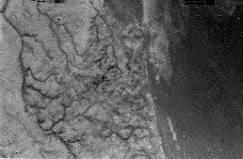
\includegraphics[max width=\linewidth]{{../images/huyghens.2}.jpg}\]
People have long suspected that Titan has lakes of made of methane
and/or ethane, but now we may be seeing them. And when Huygens landed,
its sensors reported that it broke through a crusty surface and sunk
about 20 centimeters into something mushy: probably methane mud!

The first color photo of the surface looks disappointingly like Mars at
first sight:
\[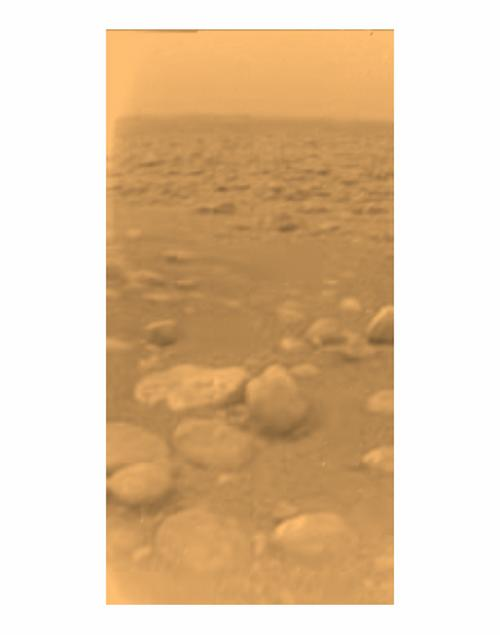
\includegraphics[max width=\linewidth]{{../images/huyghens.1}.jpg}\]
But, the surface is pumpkin-colored due to tholins or something, not
rust red. The sky is orange too! The ``rocks'' could be water ice. And
they've detected hints of volcanos that spew molten water and ammonia!
So, it's a strange new world.

Back here on Earth, there was a conference in December in honor of Larry
Breen's 60th birthday:

\begin{enumerate}
\def\labelenumi{\arabic{enumi})}
\setcounter{enumi}{1}
\tightlist
\item
  Arithmetic, Geometry and Topology: Conference on occasion of Larry
  Breen's sixtieth birthday,
  \texttt{http://www-math.univ-paris13.fr/\textasciitilde{}lb2004/}
\end{enumerate}

It was in Paris. This was my first visit to that city, but luckily I got
to stay there an extra week after the conference, so I could focus on
the math while it was going on.

But I can't resist a digression! Paris won my heart, despite my
suspicions that it had somehow been hyped all along. First of all, it's
beautiful. Second, it's nice to be someplace where people take simple
foods like bread, cheese, fruits and vegetables really seriously, and
don't settle for the tasteless crud we so often eat in the US.

None of this came as a surprise, of course. What surprised is that I've
never seen a city with so many bookstores --- and good ones, too!
They're clustered thick near the Sorbonne, but the Latin Quarter is
dotted with them, and there are even lots along the Boulevard
St-Germain, which is the biggest most fashionable shopping street. I
don't think there's any place in the English speaking world with so many
bookstores. Not London, not New York\ldots{} Cambridge Massachusetts
used to have lots near Harvard Square, back when I was a grad student,
but the high rents have long since squeezed them out, replacing bohemian
diversity with clothing shops for boring rich people, like Abercrombie
and Fitch. Somehow in Paris fancy clothing and books coexist.

Umm, but what about the conference?

Well, Breen's work is mainly on algebraic geometry a la Grothendieck,
with a strong emphasis on category theory. Beautiful stuff, and lately
it's it's begun to find applications to string theory --- especially his
work on gerbes. People at his conference spoke on all sorts of topics,
most of which I didn't understand very well --- some heavy-duty number
theory, for example. I understood a few well enough to really enjoy
them, like Mike Hopkins' talk on derived algebraic geometry, Clemens
Berger's talk on geometric Reedy categories, and Ieke Moerdijk's talk on
the homotopy theory of operads. But I won't try to explain these --- I
want to explain what a ``gerbe'' is, so I have my work cut out for me.

One way to get going on the idea of gauge theory is to start with
electromagnetism, where the concept of ``phase'' turns out to play a
crucial role. If you move a charged particle through an electromagnetic
field, its wavefunction gets multiplied by a unit complex number, or
``phase'' --- and it turns out, rather wonderfully, that all effects of
electricity and magnetism on charged particles is due to this!

However, phases are funny. You can't actually measure the phase of a
charged particle --- at least, there's no such thing as a ``phasometer''
where you stick in a particle and the dial on the meter points to a unit
complex number. Of course a unit complex number is just a fancy name for
a point on the circle, and a dial is precisely the right shape for
that\ldots{} but you just can't build this machine.

Instead, you can only measure the \emph{change} in phase of a particle
as it goes around a loop. Or, equivalently, the \emph{difference} in
phases when a particle takes two different paths from here to there.
See, in quantum mechanics you can play tricks like the ``double slit
experiment'', where you coax a particle's wavefunction to smear out and
take two routes from here to there\ldots{} and then when it arrives, it
interferes with itself, and if you're smart you can see by these
interference effects what the relative phase of the two paths is.

Pretty weird, eh? I'm so used to this that it seems completely normal to
me, but I should admit that this way of understanding the
electromagnetic field came fairly late. Weyl had a hint of it in 1918
when he invented the term ``gauge theory'' in his quest to unify
electromagnetism and gravity, but he was mixed up in some crucial ways
that only got sorted out quite a bit later. For more details, try
O'Raiferteagh's book ``The Dawning of Gauge Theory'', which I discussed
in \protect\hyperlink{week116}{``Week 116''}.

Anyway, the concept of relative phase, or difference in phase, is nicely
captured by the concept of a ``torsor''. A unit complex number is a
point on the unit circle in the complex plane. This circle is a group
since we can multiply unit complex numbers and get unit complex numbers
back. This group is called \(\mathrm{U}(1)\). Like a dial,
\(\mathrm{U}(1)\) has standard names for all the points on it --- and it
has one god-given special point, the identity element, namely the number
\(1\).

A ``\(\mathrm{U}(1)\)-torsor'' is a lot like \(\mathrm{U}(1)\), but
subtly different. It's a circle where the points aren't given these
standard names\ldots{} but where you can still tell measure angles, and
tell the difference between clockwise and counterclockwise.

You can't get an element of \(\mathrm{U}(1)\) from \emph{one} point on a
\(\mathrm{U}(1)\)-torsor. But, if you have \emph{two} points on a
\(\mathrm{U}(1)\)-torsor, you can say how much rotation it takes to get
from one to the other, and this give an element of \(\mathrm{U}(1)\). In
other words, you can describe the ``difference in phase'' between these
two points.

For more on torsors, try this:

\begin{enumerate}
\def\labelenumi{\arabic{enumi})}
\setcounter{enumi}{2}
\tightlist
\item
  John Baez, ``Torsors made easy'',
  \texttt{http://math.ucr.edu/home/baez/torsors.html}
\end{enumerate}

Anyway, the real idea behind electromagnetism is that sitting over each
point in spacetime is a \(\mathrm{U}(1)\)-torsor. If a particle is
sitting at some point in spacetime, its phase is not really a number:
it's an element of the \(\mathrm{U}(1)\)-torsor sitting over that point!
To get a \emph{number}, we have to carry the particle around a loop! Its
phase will change when we do this, so we get \emph{two} points in a
\(\mathrm{U}(1)\)-torsor, and their difference is an element of
\(\mathrm{U}(1)\).

So while it sounds far-out, the key mathematical structure in
electromagnetism is a bunch of \(\mathrm{U}(1)\)-torsors, one over each
point in spacetime. This is called a ``principal
\(\mathrm{U}(1)\)-bundle'' or sometimes just a
``\(\mathrm{U}(1)\)-bundle'' for short.

If we wanted to describe some force other than electromagnetism, we
could take this whole setup and replace \(\mathrm{U}(1)\) with some
other group. In fact, this idea works great: it's the main idea behind
gauge theories, which do an excellent job of describing all the forces
in nature.

To set up a gauge theory, the first thing you need to do is pick a group
\(G\) and pick a ``principal \(G\)-bundle'' over spacetime. Spacetime
will be some manifold \(X\). A principal \(G\)-bundle over \(X\) is
gadget that assigns a \(G\)-torsor to each point of \(X\). A
\(G\)-torsor is a space where if you pick two points in it, you get an
element of \(G\) which describes their ``difference''.

I'm being fairly sloppy here, so don't take these as precise
definitions! I give a precise definition of a \(G\)-torsor in the above
webpage, and any decent book on differential geometry will give you a
definition of a principal \(G\)-bundle. However, only rather highbrow
books define principal \(G\)-bundles with the help of
\(G\)-torsors\ldots{} which is sad, because it's not that hard, and
rather enlightening.

Anyway, in gauge theory the forces of nature are described by
``connections'' on principal \(G\)-bundles. Let's say we have a
principal \(G\)-bundle \(P\) which assigns to each point \(x\) of our
manifold a \(G\)-torsor \(P(x)\). Then a ``connection'' on \(P\) is a
gadget that says how any path from \(x\) to \(y\) gives a map from
\(P(x)\) to \(P(y)\). If \(G\) is \(\mathrm{U}(1)\), for example, this
gadget says how the phase of a charged particle changes as we move it
along any path from \(x\) to \(y\).

Now suppose we have a loop that starts and ends at \(x\). Then our
connection gives a map from \(P(x)\) to itself. If we start with a point
in \(P(x)\), and apply this map, we get another point in \(P(x)\). Since
\(P(x)\) is a \(G\)-torsor, these two points determine an element of
\(G\). This is how we get group elements from loops in gauge theory!

Now let me sketch how gerbes enter the game. First I'll do the case
where the group \(G\) is abelian, for example \(\mathrm{U}(1)\). It's
the nonabelian gerbes that really interest me\ldots{} but the abelian
case is a lot easier. The reason is that when \(G\) is abelian, the
group element we get in the previous paragraph doesn't depend on the
choice of a point of \(P(x)\).

Gerbes show up when we try to invent a kind of ``higher gauge theory''
that describes how not just point particles but \(1\)-dimensional
objects transform when you move them around. For example, the strings in
string theory, or the loops in loop quantum gravity.

This leads to a mind-boggling self-referential twist, which is just the
kind of thing I love:

As we've seen, a connection describes how a point particle transforms
when you carry it along a path: \[
  \begin{gathered}
    x\xrightarrow{f}y
  \\[1em]\mbox{a path $f$ from the point $x$ to the point $y$;}
  \\\mbox{we write this as $f\colon x\to y$.}
  \end{gathered}
\] Now we need a gadget that'll describe how a \emph{path} transforms
when you carry it along a \emph{path of paths:} \[
  \begin{gathered}
    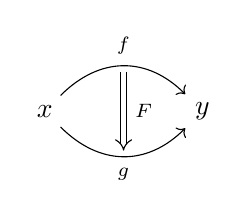
\begin{tikzpicture}
      \node (x) at (0,0) {$x$};
      \node (y) at (2,0) {$y$};
      \draw[->] (x) .. node[label={[label distance=-1mm]above:{\scriptsize$f$}}]{} controls (0.7,0.7) and (1.3,0.7) .. (y);
      \draw[->] (x) .. node[label={[label distance=-1mm]below:{\scriptsize$g$}}]{}controls (0.7,-0.7) and (1.3,-0.7) .. (y);
      \draw[double,double equal sign distance,-implies] (1,0.5) to node[label={[label distance=-1mm]right:{\scriptsize$F$}}]{} (1,-0.5);
    \end{tikzpicture}
  \\[1em]\mbox{a path $f$ from the point $x$ to the point $y$;}
  \\\mbox{we write this as $f\colon x\to y$.}
  \end{gathered}
\] To do this, we need to boost our level of thinking a notch, working
not with ``\(G\)-torsors'' and ``principal \(G\)-bundles'' but instead
with ``\(G\)-\(2\)-torsors'' and ``\(G\)-gerbes''.

Here's how it goes:

We start by picking an abelian group \(G\) and a manifold \(X\).

Then we pick a ``\(G\)-gerbe'' over \(X\), say \(P\).

What's that? It's a thing that assigns to each point \(x\) of \(X\) a
``\(G\)-\(2\)-torsor'', say \(P(x)\).

What's that? Well, it's a thing where if you pick two points in it, you
get a \emph{\(G\)-torsor} describing their difference!

Get it? This is the beginning of a story that goes on forever:

\begin{itemize}
\tightlist
\item
  Two points in a \(G\)-torsor determine an element of \(G\);
\item
  two points in a \(G\)-\(2\)-torsor determine a \(G\)-torsor;
\item
  two points in a \(G\)-\(3\)-torsor determine a \(G\)-\(2\)-torsor;
\item
  \ldots{}
\end{itemize}

But, you'll probably be relieved to know we won't go beyond
\(G\)-\(2\)-torsors today.

Next, we pick a ``connection'' on \(P\).

What's that? Well, it's a gadget that for each path from \(x\) to \(y\)
gives us a map from the \(G\)-\(2\)-torsor \(P(x)\) to the
\(G\)-\(2\)-torsor \(P(y)\). If we call the path \[f\colon x \to y\]
then we call this map \[P(f)\colon P(x) \to P(y)\] Moroever, this sort
of connection also gives a ``map between maps'' for each path-of-paths!
So, from \[F\colon f \Rightarrow g\] it gives
\[P(F)\colon P(f) \Rightarrow P(g)\]

I haven't explained enough stuff to say yet what these ``maps between
maps'' are, so let's just see what happens if we have a loop
\[f\colon x \to x\] and then a loop-of-loops \[F\colon f \Rightarrow f\]
From the loop \(f\colon x \to x\), our connection gives us a map:
\[P(f)\colon P(x) \to P(x)\] If we start with a point in \(P(x)\), and
apply this map, we get another point in \(P(x)\). Since \(P(x)\) is a
\(G\)-\(2\)-torsor, these two points determine a \(G\)-torsor. This
\(G\)-torsor doesn't depend on our initial choice of point, and it
completely determines the map \(P(f)\). So, we can think of \(P(f)\) as
\emph{being} this \(G\)-torsor, if we like.

From the loop-of-loops \(F\colon f \Rightarrow f\), our connection gives
us a map: \[P(F)\colon P(f) \Rightarrow P(f)\] If we start with a point
in \(P(f)\), and apply this map, we get another point. Since \(P(f)\) is
a \(G\)-torsor, these two points determine an element of \(G\). This
element of \(G\) doesn't depend on our initial choice of point, and it
completely determines the map \(P(F)\). So, we can think of \(P(F)\) as
\emph{being} this element of \(G\), if we like.

In short, the machinery functions just as you'd hope, giving a group
element that describes how a loop of string ``changes phase'' as you
carry it around a loop-of-loops!

So far I've been strenously avoiding the language of categories and
\(2\)-categories, but if you're at all familiar with that language,
you'll have guessed that it's precisely what we need to make everything
I'm saying precise.

It's actually incredibly beautiful\ldots{} but I'm getting lazy, so I'll
explain it very tersely now, in a way that only true lovers of
abstraction will enjoy:

If \(G\) is a group, it acts on itself by left translation. So, it
becomes a left \(G\)-set. Any left \(G\)-set isomorphic to this one is
called a ``\(G\)-torsor''. There's a category \(G\)-\(\mathsf{Tor}\)
whose objects are \(G\)-torsors and whose morphisms are maps compatible
with the action of \(G\). Since all \(G\)-torsors are isomorphic, and
the automorphism group of any one is just \(G\), this category
\(G\)-\(\mathsf{Tor}\) is equivalent to \(G\) (regarded as a
\(1\)-object category).

If \(G\) is abelian, every left \(G\)-set becomes a right \(G\)-set too.
This allows us to define a ``tensor product'' of \(G\)-sets. The tensor
product of \(G\)-torsors is a \(G\)-torsor, so \(G\)-\(\mathsf{Tor}\)
becomes a monoidal category. In fact, it's a ``\(2\)-group'': a monoidal
category where all the objects and morphisms are invertible.

This allows us to iterate what we've just done:

Since \(G\)-\(\mathsf{Tor}\) is a \(2\)-group, it acts on itself by left
translation. So, it becomes a ``left \(G\)-category''. Any left
\(G\)-category isomorphic to this one is called a
``\(G\)-\(2\)-torsor''. There's a \(2\)-category
\(G\)-\(2\)-\(\mathsf{Tor}\) whose objects are \(G\)-\(2\)-torsors,
whose morphisms are functors compatible the action of \(G\), and whose
morphisms are natural transformations compatible with the action of
\(G\). Since all \(G\)-\(2\)-torsors are isomorphic, any the
automorphism \(2\)-group of any one is just \(G\)-\(\mathsf{Tor}\), this
\(2\)-category is equivalent to \(G\)-\(\mathsf{Tor}\) (regarded as a
\(1\)-object \(2\)-category).

And so on! This infinite hierarchy only works when \(G\) is abelian;
when \(G\) is nonabelian we need a different hierarchy, which uses
``bitorsors'', where \(G\) acts on both left and right, instead of
``torsors''.

To learn more about this stuff, here are some references. I'll stick to
ones I didn't already list in \protect\hyperlink{week71}{``Week 71''}
and \protect\hyperlink{week151}{``Week 151''}.

First, for physicists, some work on the role of gerbes and \(2\)-gerbes
in string theory and M-theory:

\begin{enumerate}
\def\labelenumi{\arabic{enumi})}
\setcounter{enumi}{3}
\item
  Paolo Aschieri, Luigi Cantini and Branislav Jurco, ``Nonabelian bundle
  gerbes, their differential geometry and gauge theory'', available as
  \href{https://arxiv.org/abs/hep-th/0312154}{\texttt{hep-th/0312154}}.
\item
  Paolo Aschieri and Branislav Jurco, ``Gerbes, M5-brane anomalies and
  \(\mathrm{E}_8\) gauge theory'', available as
  \href{https://arxiv.org/abs/hep-th/0409200}{\texttt{hep-th/0409200}}.
\end{enumerate}

Second, for mathematicians, some classic works by Breen:

\begin{enumerate}
\def\labelenumi{\arabic{enumi})}
\setcounter{enumi}{5}
\item
  Lawrence Breen, ``Bitorseurs et cohomologie non-abelienne'', in
  \emph{The Grothendieck Festschrift}, eds.~P. Cartier et al, Progress
  in Mathematics vol.~\textbf{86}, Birkhauser, Boston, 1990,
  pp.~401--476.
\item
  Lawrence Breen, ``Theorie de Schreier superieure'', \emph{Ann. Sci.
  Ecole Norm. Sup.} \textbf{25} (1992), 465--514.
\item
  Lawrence Breen, ``Classification of \(2\)-stacks and \(2\)-gerbes'',
  \emph{Asterisque} \textbf{225}, Societe Mathematique de France, 1994.
\end{enumerate}

\(2\)-gerbes are what you get if you climb the hierarchy one more step.
They should be good for describing the parallel transport of
\(2\)-dimensional surfaces, or ``\(2\)-branes'' --- and indeed they make
an appearance in Aschieri and Jurco's paper for precisely that reason.

Another key reference is Breen's paper with Messing about connections on
nonabelian gerbes:

\begin{enumerate}
\def\labelenumi{\arabic{enumi})}
\setcounter{enumi}{8}
\tightlist
\item
  Lawrence Breen and William Messing, ``The differential geometry of
  gerbes'', available as
  \href{http://www.arXiv.org/abs/math.AG/0106083}{\texttt{math.AG/0106083}}.
\end{enumerate}

and Breen's lecture notes from the IMA workshop on higher categories:

\begin{enumerate}
\def\labelenumi{\arabic{enumi})}
\setcounter{enumi}{9}
\tightlist
\item
  Larry Breen, ``\(n\)-Stacks and \(n\)-gerbes: homotopy theory''. Notes
  available at \texttt{http://www.ima.umn.edu/categories/\#thur}
\end{enumerate}

I've been working on this stuff myself lately, from a somewhat different
viewpoint. So far I've written papers with Aaron Lauda and Alissa Crans
about \(2\)-groups and Lie \(2\)-algebras:

\begin{enumerate}
\def\labelenumi{\arabic{enumi})}
\setcounter{enumi}{10}
\item
  John Baez and Aaron Lauda, ``Higher-dimensional algebra V:
  \(2\)-groups'', \emph{Theory and Applications of Categories}
  \textbf{12} (2004), 423--491. Available online at
  \texttt{http://www.tac.mta.ca/tac/volumes/12/14/12-14abs.html} or as
  \href{http://www.arXiv.org/abs/math.QA/0307200}{\texttt{math.QA/0307200}}.
\item
  John Baez and Alissa Crans, ``Higher-dimensional algebra VI: Lie
  \(2\)-algebras'', \emph{Theory and Applications of Categories}
  \textbf{12} (2004), 492--528. Available online at
  \texttt{http://www.tac.mta.ca/tac/volumes/12/15/12-15abs.html} or as
  \href{http://www.arXiv.org/abs/math.QA/0307263}{\texttt{math.QA/0307263}}.
\end{enumerate}

Aaron Lauda was getting a masters degree in physics at UCR when we
started our paper on \(2\)-groups. Now he's a grad student in math at
the University of Cambridge, working on things related to topological
quantum field theory with the category theorist Martin Hyland. Alissa
Crans did her PhD in math at UCR, and our paper on Lie \(2\)-algebras
contains a lot of stuff from her thesis. Now she has a job at Loyola
Marymount University, in Los Angeles.

I've had a huge amount of fun working with both of them! Luckily Alissa
lives nearby, and I visit Cambridge most summers. So, we can all keep
working on other projects together --- and we are.

I also have some gerbe-related projects going on with my grad student
Toby Bartels, Danny Stevenson (who is teaching at UCR now) and Urs
Schreiber, a fellow moderator of \texttt{sci.physics.research} who will
soon be a postdoc at Hamburg with Christoph Schweigert. Urs will be
visiting UCR for two weeks in February, and we plan to figure a lot of
stuff out. So, I've got gerbes on the brain, and I'll probably be saying
more about them in the future, unless I burn up all my expository energy
writing papers.

In fact, one of the best places to learn about the differential geometry
of abelian gerbes and \(2\)-gerbes is Danny's thesis:

\begin{enumerate}
\def\labelenumi{\arabic{enumi})}
\setcounter{enumi}{12}
\tightlist
\item
  Danny Stevenson, \emph{The geometry of bundle gerbes}, Ph.D.~thesis,
  University of Adelaide, 2000. Available as
  \href{http://www.arXiv.org/abs/math.DG/0004117}{\texttt{math.DG/0004117}}.
\end{enumerate}

He's also written lots of other papers on gerbes, which you can find on
the arXiv. Physicists may find these the most interesting:

\begin{enumerate}
\def\labelenumi{\arabic{enumi})}
\setcounter{enumi}{13}
\item
  Michael K. Murray and Danny Stevenson, ``Higgs fields, bundle gerbes
  and string structures'', \emph{Comm. Math. Phys.} \textbf{236} (2003),
  541--555. Also available as
  \href{http://www.arXiv.org/abs/math.DG/0106179}{\texttt{math.DG/0106179}}.
\item
  Alan L. Carey, Stuart Johnson, Michael K. Murray, Danny Stevenson and
  Bai-Ling Wang, ``Bundle gerbes for Chern-Simons and Wess-Zumino-Witten
  models'', available as
  \href{http://www.arXiv.org/abs/math.DG/0410013}{\texttt{math.DG/0410013}}.
\end{enumerate}

Toby is doing his thesis on categorified bundles, or ``\(2\)-bundles'',
and you can already get a preview here:

\begin{enumerate}
\def\labelenumi{\arabic{enumi})}
\setcounter{enumi}{15}
\tightlist
\item
  Toby Bartels, ``Categorified gauge theory: \(2\)-bundles'', available
  as
  \href{http://www.arXiv.org/abs/math.CT/0410328}{\texttt{math.CT/0410328}}.
\end{enumerate}

\(2\)-bundles are meant to be an alternative to gerbes: although I've
done my best to hide it above, a gerbe is really more like a
categorified \emph{sheaf} than a bundle. And, just as a bundle has a
sheaf of sections, we're hoping that a \(2\)-bundle has a stack of
sections, which in certain cases will be a gerbe. That's one of the
things we need to figure out, though.

And, while I'm listing the papers of the gerbe gang, I should admit that
Urs and I have written a paper about connections on \(2\)-bundles. But,
I want to polish this paper a bit before talking about it here.

As for \(2\)-groups, various people have been studying their
representations lately, and this should become an important part of
higher gauge theory, just as group representations are crucial in gauge
theory:

\begin{enumerate}
\def\labelenumi{\arabic{enumi})}
\setcounter{enumi}{16}
\item
  Magnus Forrester-Barker, \emph{Representations of crossed modules and
  cat\textsuperscript{1}-groups}, Ph.D.~thesis, Department of
  Mathematics, University of Wales, Bangor, 2004. Available at
  \texttt{http://www.maths.bangor.ac.uk/research/ftp/theses/forrester-barker.pdf}
\item
  John Barrett and Marco Mackaay, ``Categorical representations of
  categorical groups'', available as
  \href{http://www.arXiv.org/abs/math.CT/0407463}{\texttt{math.CT/0407463}}.
\item
  Josep Elgueta, ``Representation theory of \(2\)-groups on finite
  dimensional \(2\)-vector spaces'', available as
  \href{http://www.arXiv.org/abs/math.CT/0408120}{\texttt{math.CT/0408120}}.
\item
  Louis Crane and David Yetter, ``Measurable categories and
  \(2\)-groups'', available as
  \href{http://www.arXiv.org/abs/math.QA/0305176}{\texttt{math.QA/0305176}}.
\item
  David Yetter, ``Measurable categories'', available as
  \href{http://www.arXiv.org/abs/math.CT/0309185}{\texttt{math.CT/0309185}}.
\item
  Louis Crane and Marnie D. Sheppeard, ``\(2\)-categorical Poincare
  representations and state sum applications'', available as
  \href{http://www.arXiv.org/abs/math.QA/0306440}{\texttt{math.QA/0306440}}.
\end{enumerate}

Hendryk Pfeiffer's papers on higher gauge theory are also very
interesting. Since he works on lattice gauge theory and spin foam
models, the first two papers here develop higher gauge theory on a
discrete spacetime, and then compare it to higher gauge theory on a
manifold:

\begin{enumerate}
\def\labelenumi{\arabic{enumi})}
\setcounter{enumi}{22}
\item
  Hendryk Pfeiffer, ``Higher gauge theory and a non-Abelian
  generalization of \(2\)-form electrodynamics'', \emph{Annals Phys.}
  \textbf{308} (2003), 447--477. Also available as
  \href{https://arxiv.org/abs/hep-th/0304074}{\texttt{hep-th/0304074}}.
\item
  Florian Girelli and Hendryk Pfeiffer, ``Higher gauge theory ---
  differential versus integral formulation'', \emph{Jour. Math. Phys.}
  \textbf{45} (2004), 3949--3971. Also available as
  \href{https://arxiv.org/abs/hep-th/0309173}{\texttt{hep-th/0309173}}.
\item
  Hendryk Pfeiffer, ``\(2\)-groups, trialgebras and their Hopf
  categories of representations'', available as
  \href{http://www.arXiv.org/abs/math.QA/0411468}{\texttt{math.QA/0411468}}.
\end{enumerate}

The third one partially fulfills an old dream of Crane and Frenkel --- a
dream I vaguely hinted at way back in \protect\hyperlink{week50}{``Week
50''}. Their dream was to find a concept of ``trialgebra'' such that a
trialgebra has a Hopf category of representations, which in turn can
have a monoidal \(2\)-category of representations of its own. This is a
kind of aggravated version of a pattern already familiar in algebra,
where a Hopf algebra (or bialgebra) has a monoidal category of
representations.

Pfeiffer doesn't define general trialgebras, but only ``cocommutative
trialgebras'' and ``commutative cotrialgebras''. A cocommutative
trialgebra is a category in the category of cocommutative Hopf algebras,
while a commutative cotrialgebra is a category in the opposite of the
category of commutative Hopf algebras. Zounds --- say that three times
fast!

He shows you can get these two gadgets from \(2\)-groups in analogy to
how you get cocommutative or commutative Hopf algebras from groups, by
taking the group algebra or the algebra of functions on a group. He also
proves a Tannaka- Krein theorem that lets you reconstruct commutative
cotrialgebras from their Hopf categories of representations.

Really cool stuff!

By the way, here are some photos of Larry Breen's conference, and of
Paris:

\begin{enumerate}
\def\labelenumi{\arabic{enumi})}
\setcounter{enumi}{25}
\tightlist
\item
  John Baez, Paris, \texttt{http://math.ucr.edu/home/baez/paris/}
\end{enumerate}

\begin{center}\rule{0.5\linewidth}{0.5pt}\end{center}



\hypertarget{week211}{%
\section{March 6, 2005}\label{week211}}

The last time I wrote an issue of this column, the Huyghens probe was
bringing back cool photos of Titan. Now the European ``Mars Express''
probe is bringing back cool photos of Mars!

\begin{enumerate}
\def\labelenumi{\arabic{enumi})}
\tightlist
\item
  Mars Express website,
  \texttt{http://www.esa.int/SPECIALS/Mars\_Express/index.html}
\end{enumerate}

There are some tantalizing pictures of what might be a ``frozen sea''
--- water ice covered with dust --- near the equator in the Elysium
Planitia region:
\[\href{http://www.esa.int/SPECIALS/Mars_Express/SEMCHPYEM4E_0.html}{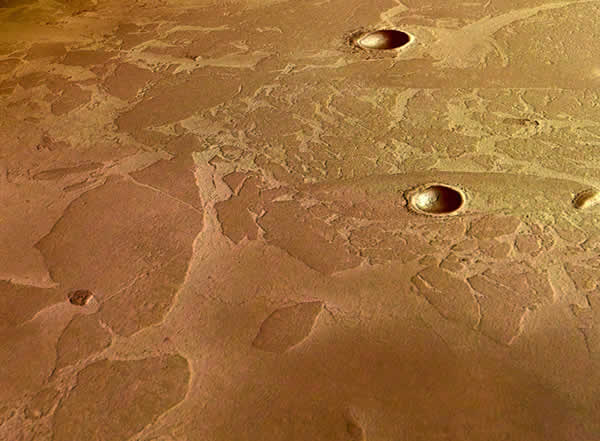
\includegraphics[max width=\linewidth]{../images/mars_packice.jpg}}\]

\begin{enumerate}
\def\labelenumi{\arabic{enumi})}
\setcounter{enumi}{1}
\tightlist
\item
  Mars Express sees signs of a ``frozen sea'',
  \texttt{http://www.esa.int/SPECIALS/Mars\_Express/SEMCHPYEM4E\_0.html}
\end{enumerate}

Ice has already been found at the Martian poles --- it's easily visible
there, and Mars Express is getting some amazing closeups of it now -
here's a here's a view of some ice on sand at the north pole:
\[\href{http://www.esa.int/SPECIALS/Mars_Express/SEMLF6D3M5E_1.html}{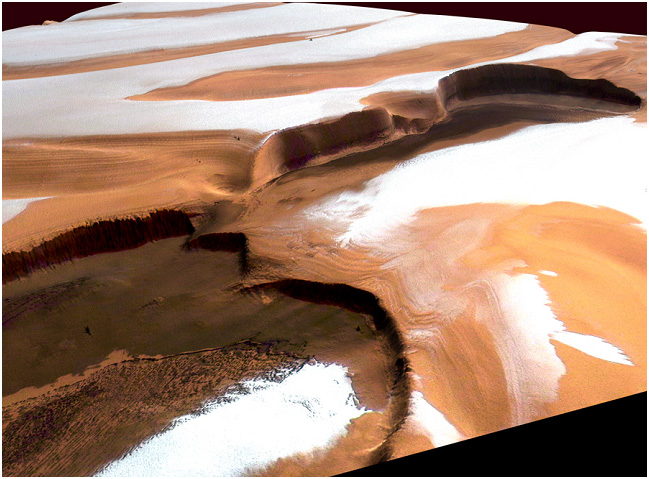
\includegraphics[max width=\linewidth]{../images/mars_pole.jpg}}\]

\begin{enumerate}
\def\labelenumi{\arabic{enumi})}
\setcounter{enumi}{2}
\tightlist
\item
  Glacial, volcanic and fluvial activity on Mars: latest images,
  \texttt{http://www.esa.int/SPECIALS/Mars\_Express/SEMLF6D3M5E\_1.html}
\end{enumerate}

What's new is the possibility of large amounts of water in warmer parts
of the planet.

Now for some math. It's always great when two subjects you're interested
in turn out to be bits of the same big picture. That's why I've been
really excited lately about Bott periodicity and the ``super-Brauer
group''.

I wrote about Bott periodicity in \protect\hyperlink{week105}{``Week
105''}, and about the Brauer group in \protect\hyperlink{week209}{``Week
209''}, but I should remind you about them before putting them together.

Bott periodicity is all about how math and physics in n+8-dimensional
space resemble math and physics in \(n\)-dimensional space. It's a weird
and wonderful pattern that you'd never guess without doing some
calculations. It shows up in many guises, which turn out to all be
related. The simplest one to verify is the pattern of Clifford algebras.

You're probably used to the complex numbers, where you throw in just
\emph{one} square root of \(-1\), called \(i\). And maybe you've heard
of the quaternions, where you throw in \emph{two} square roots of
\(-1\), called \(i\) and \(j\), and demand that they anticommute:
\[ij = -ji\] This implies that \(k = ij\) is another square root of
\(-1\). Try it and see!

In the late 1800s, Clifford realized there's no need to stop here. He
invented what we now call the ``Clifford algebras'' by starting with the
real numbers and throwing in n square roots of \(-1\), all of which
anticommute with each other. The result is closely related to rotations
in \(n+1\) dimensions, as I explained in
\protect\hyperlink{week82}{``Week 82''}.

I'm not sure who first worked out all the Clifford algebras --- perhaps
it was Cartan --- but the interesting fact is that they follow a
periodic pattern. If we use \(C_n\) to stand for the Clifford algebra
generated by n anticommuting square roots of \(-1\), they go like this:

\begin{longtable}[]{@{}ll@{}}
\toprule
\(n\) & \(C_n\)\tabularnewline
\midrule
\endhead
\(0\) & \(\mathbb{R}\)\tabularnewline
\(1\) & \(\mathbb{C}\)\tabularnewline
\(2\) & \(\mathbb{H}\)\tabularnewline
\(3\) & \(\mathbb{H}\oplus\mathbb{H}\)\tabularnewline
\(4\) & \(\mathbb{H}(2)\)\tabularnewline
\(5\) & \(\mathbb{C}(4)\)\tabularnewline
\(6\) & \(\mathbb{R}(8)\)\tabularnewline
\(7\) & \(\mathbb{R}(8)\oplus\mathbb{R}(8)\)\tabularnewline
\bottomrule
\end{longtable}

where:

\begin{itemize}
\tightlist
\item
  \(\mathbb{R}(n)\) means \(n \times n\) real matrices,
\item
  \(\mathbb{C}(n)\) means \(n \times n\) complex matrices, and
\item
  \(\mathbb{H}(n)\) means \(n \times n\) quaternionic matrices.
\end{itemize}

All these become algebras with the usual addition and multiplication of
matrices. Finally, if \(A\) is an algebra, \(A \oplus A\) consists of
pairs of guys in \(A\), with pairwise addition and multiplication.

What happens next? Well, from then on things sort of ``repeat'' with
period 8: \(C_{n+8}\) consists of \(16 \times 16\) matrices whose
entries lie in \(C_n\)!

So, you can remember all the Clifford algebras with the help of this
eight-hour clock: \[
  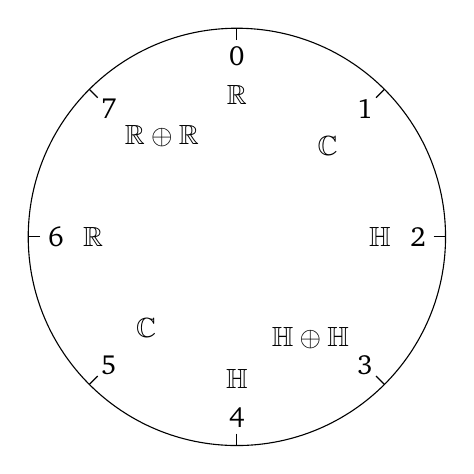
\begin{tikzpicture}
    \draw (0,0) circle[radius=2.65cm];
    \node[label=below:{$\mathbb{R}$}] at (90:2.3) {0};
    \node[label=below left:{$\mathbb{C}$}] at (45:2.3) {1};
    \node[label=left:{$\mathbb{H}$}] at (0:2.3) {2};
    \node[label={[label distance=-2mm]above left:{$\mathbb{H}\oplus\mathbb{H}$}}] at (-45:2.3) {3};
    \node[label=above:{$\mathbb{H}$}] at (-90:2.3) {4};
    \node[label=above right:{$\mathbb{C}$}] at (-135:2.3) {5};
    \node[label=right:{$\mathbb{R}$}] at (180:2.3) {6};
    \node[label={[label distance=-2mm]below right:{$\mathbb{R}\oplus\mathbb{R}$}}] at (135:2.3) {7};
    \foreach \a in {0,45,90,135,180,-135,-90,-45}
      \draw (\a:2.5) to (\a:2.65);
  \end{tikzpicture}
\] To use this clock, you have to remember to use matrices of the right
size to get \(C_n\) to have dimension \(2^n\). So, when I write
``\(\mathbb{R}\oplus\mathbb{R}\)'' next to the ``7'' on the clock, I
don't mean \(C_7\) is really \(\mathbb{R}\oplus\mathbb{R}\). To get
\(C_7\), you have to take \(\mathbb{R}\oplus\mathbb{R}\) and beef it up
until it becomes an algebra of dimension \(2^7 = 128\). You do this by
taking \(\mathbb{R}(8)\oplus\mathbb{R}(8)\), since this has dimension
\(8\times8 + 8\times8 = 128\).

Similarly, to get \(C_{10}\), you note that 10 is 2 modulo 8, so you
look at ``2'' on the clock and see ``\(\mathbb{H}\)'' next to it,
meaning the quaternions. But to get \(C_{10}\), you have to take
\(\mathbb{H}\) and beef it up until it becomes an algebra of dimension
\(2^{10} = 1024\). You do this by taking \(\mathbb{H}(16)\), since this
has dimension \(4\times16\times16 = 1024\).

This ``beefing up'' process is actually quite interesting. For any
associative algebra \(A\), the algebra \(A(n)\) consisting of
\(n \times n\) matrices with entries in \(A\) is a lot like \(A\)
itself. The reason is that they have equivalent categories of
representations!

To see what I mean by this, remember that a ``representation'' of an
algebra is a way for its elements to act as linear transformations of
some vector space. For example, \(\mathbb{R}(n)\) acts as linear
transformations of \(\mathbb{R}^n\) by matrix multiplication, so we say
\(\mathbb{R}(n)\) has a representation on \(R^n\). More generally, for
any algebra \(A\), the algebra \(A(n)\) has a representation on \(A^n\).

More generally still, if we have any representation of \(A\) on a vector
space \(V\), we get a representation of \(A(n)\) on \(V^n\). It's less
obvious, but true, that \emph{every} representation of \(A(n)\) comes
from a representation of \(A\) this way.

In short, just as \(n \times n\) matrices with entries in \(A\) form an
algebra \(A(n)\) that's a beefed-up version of \(A\) itself, every
representation of \(A(n)\) is a beefed-up version of some representation
of \(A\).

Even better, the same sort of thing is true for maps between
representations of \(A(n)\). This is what we mean by saying that
\(A(n)\) and \(A\) have equivalent categories of representations. If you
just look at the categories of representations of these two algebras as
abstract categories, there's no way to tell them apart! We say two
algebras are ``Morita equivalent'' when this happens.

It's fun to study Morita equivalence classes of algebras --- say
algebras over the real numbers, for example. The tensor product of
algebras gives us a way to multiply these classes. If we just consider
the invertible classes, we get a \emph{group}. This is called the
``Brauer group'' of the real numbers.

The Brauer group of the real numbers is just \(\mathbb{Z}/2\),
consisting of the classes \([\mathbb{R}]\) and \([\mathbb{H}]\). These
correspond to the top and bottom of the Clifford clock! Part of the
reason is that \[\mathbb{H}\otimes\mathbb{H} = \mathbb{R}(4)\] so when
we take Morita equivalence classes we get
\[[\mathbb{H}]\times[\mathbb{H}] = [\mathbb{R}]\] But, you may wonder
where the complex numbers went! Alas, the Morita equivalence class
\([\mathbb{C}]\) isn't invertible, so it doesn't live in the Brauer
group. In fact, we have this little multiplication table for tensor
product of algebras:

\begin{longtable}[]{@{}lccc@{}}
\toprule
\(\otimes\) & \(\mathbb{R}\) & \(\mathbb{C}\) &
\(\mathbb{H}\)\tabularnewline
\midrule
\endhead
\(\mathbb{R}\) & \(\mathbb{R}\) & \(\mathbb{C}\) &
\(\mathbb{H}\)\tabularnewline
\(\mathbb{C}\) & \(\mathbb{C}\) & \(\mathbb{C}\oplus\mathbb{C}\) &
\(\mathbb{C}(2)\)\tabularnewline
\(\mathbb{H}\) & \(\mathbb{H}\) & \(\mathbb{C}(2)\) &
\(\mathbb{R}(4)\)\tabularnewline
\bottomrule
\end{longtable}

Anyone with an algebraic bone in their body should spend an afternoon
figuring out how this works! But I won't explain it now.

Instead, I'll just note that the complex numbers are very aggressive and
infectious --- tensor anything with a \(\mathbb{C}\) in it and you get
more \(\mathbb{C}\)'s. That's because they're a field in their own right
--- and that's why they don't live in the Brauer group of the real
numbers.

They do, however, live in the \emph{super-Brauer} group of the real
numbers, which is \(\mathbb{Z}/8\) --- the Clifford clock itself!

But before I explain that, I want to show you what the categories of
representations of the Clifford algebras look like: \[
  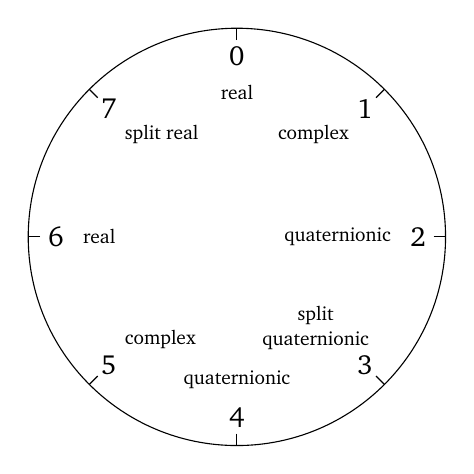
\begin{tikzpicture}
    \draw (0,0) circle[radius=2.65cm];
    \node[label=below:{\scriptsize real}] at (90:2.3) {0};
    \node[label={[label distance=-2mm]below left:{\scriptsize complex}}] at (45:2.3) {1};
    \node[label=left:{\scriptsize quaternionic}] at (0:2.3) {2};
    \node at (-45:2.3) {3};
    \node at (1,-1) {\scriptsize split};
    \node at (1,-1.32) {\scriptsize quaternionic};
    \node[label=above:{\scriptsize quaternionic}] at (-90:2.3) {4};
    \node[label={[label distance=-2mm]above right:{\scriptsize complex}}] at (-135:2.3) {5};
    \node[label=right:{\scriptsize real}] at (180:2.3) {6};
    \node[label={[label distance=-2mm]below right:{\scriptsize split real}}] at (135:2.3) {7};
    \foreach \a in {0,45,90,135,180,-135,-90,-45}
      \draw (\a:2.5) to (\a:2.65);
  \end{tikzpicture}
\] Here, the labels at each hour describe the type of vector space,
e.g.~at 3-o'clock we have split quaternionic vector spaces.

You can read this information off the 8-hour Clifford clock I showed you
before, at least if you know some stuff:

\begin{itemize}
\tightlist
\item
  A real vector space is just something like \(\mathbb{R}^n\)
\item
  A complex vector space is just something like \(\mathbb{C}^n\)
\item
  A quaternionic vector space is just something like \(\mathbb{H}^n\)
\end{itemize}

and a ``split'' vector space is a vector space that's been written as
the direct sum of two subspaces.

Take \(C_4\), for example --- the Clifford algebra generated by 4
anticommuting square roots of \(-1\). The Clifford clock tells us this
is \(\mathbb{H}\oplus\mathbb{H}\). And if you think about it, a
representation of this is just a pair of representations of
\(\mathbb{H}\). So, it's two quaternionic vector spaces --- or if you
prefer, a ``split'' quaternionic vector space.

Or take \(C_7\). The Clifford clock says this is
\(\mathbb{R}\oplus\mathbb{R}\)\ldots{} or at least Morita equivalent to
\(\mathbb{R}\oplus\mathbb{R}\): it's actually
\(\mathbb{R}(8)\oplus\mathbb{R}(8)\), but that's just a beefed-up
version of \(\mathbb{R}\oplus\mathbb{R}\), with an equivalent category
of representations. So, the category of representations of \(C_7\) is
\emph{equivalent} to the category of split real vector spaces.

And so on. Note that when we loop all the way around the clock, our
Clifford algebra becomes \(16\times16\) matrices of what it was before,
but this is Morita equivalent to what it was. So, we have a truly
period-8 clock of categories!

But here's the really cool part: there are also arrows going clockwise
and counterclockwise around this clock! Arrows between categories are
called ``functors''.

Each Clifford algebra is contained in the next one, since they're built
by throwing in more and more square roots of \(-1\). So, if we have a
representation of \(C_n\), it gives us a representation of \(C_{n-1}\).
Ditto for maps between representations. So, we get a functor from the
category of representations of \(C_n\) to the category of
representations of \(C_{n-1}\). This is called a ``forgetful functor'',
since it ``forgets'' that we have representations of \(C_n\) and just
thinks of them as representations of \(C_{n-1}\).

So, we have forgetful functors cycling around counterclockwise!

Even better, all these forgetful functors have ``left adjoints'' going
back the other way. I talked about left adjoints in
\protect\hyperlink{week77}{``Week 77''}, so I won't say much about them
now. I'll just give an example.

Here's a forgetful functor:
\[\mbox{complex vector spaces}\xrightarrow{\mbox{\scriptsize forget complex structure}}\mbox{real vector spaces}\]
which is one of the counterclockwise arrows on the Clifford clock. This
functor takes a complex vector space and forgets your ability to
multiply vectors by \(i\), thus getting a real vector space. When you do
this to \(\mathbb{C}^n\), you get \(\mathbb{R}^{2n}\).

This functor has a left adjoint:
\[\mbox{complex vector spaces}\xleftarrow{\mbox{\scriptsize complexify}}\mbox{real vector spaces}\]
where you take a real vector space and ``complexify'' it by tensoring it
with the complex numbers. When you do this to \(\mathbb{R}^n\), you get
\(\mathbb{C}^n\).

So, we get a beautiful version of the Clifford clock with forgetful
functors cycling around counterclockwise and their left adjoints cycling
around clockwise! When I realized this, I drew a big picture of it in my
math notebook --- I always carry around a notebook for precisely this
sort of thing. Unfortunately, it's a bit hard to draw this chart in
ASCII, so I won't include it here.

Instead, I'll draw something easier. For this, note the following
mystical fact: the Clifford clock is symmetrical under reflection around
the 3-o'clock/7-o'clock axis. It seems bizarre at first that it's
symmetrical along \emph{this} axis instead of the more obvious
0-o'clock/4-o'clock axis. But there's a good reason, which I already
mentioned: the Clifford algebra \(C_n\) is related to rotations in
\(n+1\) dimensions.

I would be very happy if you had enough patience to listen to a full
explanation of this fact, along with everything else I want to say. But
I bet you don't\ldots{} so I'll hasten on to the really cool stuff.

First of all, using this symmetry we can fold the Clifford clock in
half\ldots{} and the forgetful functors on one side perfectly match
their left adjoints on the other side!

So, we can save space by drawing this ``folded'' Clifford clock: \[
  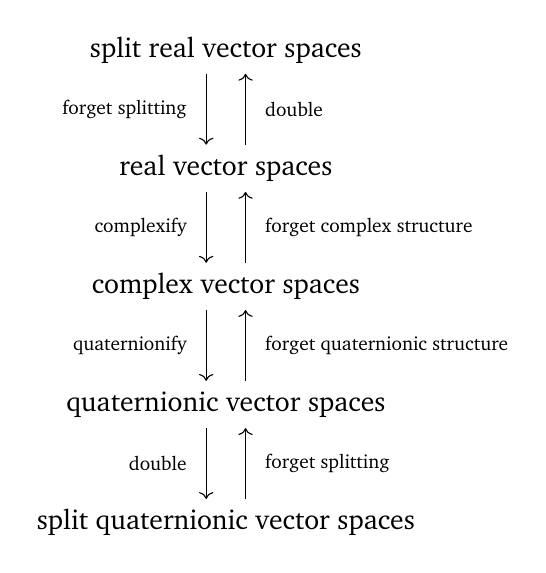
\begin{tikzpicture}[yscale=1.5]
    \node at (0,0) {split real vector spaces};
    \draw[->] (-0.25,-0.2) to node[label=left:{\scriptsize forget splitting}]{} (-0.25,-0.8);
    \draw[<-] (0.25,-0.2) to node[label=right:{\scriptsize double}]{} (0.25,-0.8);
    \node at (0,-1) {real vector spaces};
    \draw[->] (-0.25,-1.2) to node[label=left:{\scriptsize complexify}]{} (-0.25,-1.8);
    \draw[<-] (0.25,-1.2) to node[label=right:{\scriptsize forget complex structure}]{} (0.25,-1.8);
    \node at (0,-2) {complex vector spaces};
    \draw[->] (-0.25,-2.2) to node[label=left:{\scriptsize quaternionify}]{} (-0.25,-2.8);
    \draw[<-] (0.25,-2.2) to node[label=right:{\scriptsize forget quaternionic structure}]{} (0.25,-2.8);
    \node at (0,-3) {quaternionic vector spaces};
    \draw[->] (-0.25,-3.2) to node[label=left:{\scriptsize double}]{} (-0.25,-3.8);
    \draw[<-] (0.25,-3.2) to node[label=right:{\scriptsize forget splitting}]{} (0.25,-3.8);
    \node at (0,-4) {split quaternionic vector spaces};
  \end{tikzpicture}
\] The forgetful functors march downwards on the right, and their left
adjoints march back up on the left!

The arrows going between 7 o'clock and 0 o'clock look a bit weird: \[
  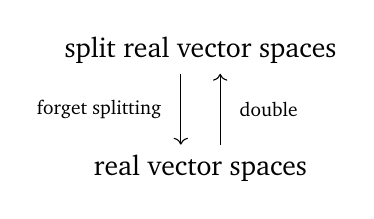
\begin{tikzpicture}[yscale=1.5]
    \node at (0,0) {split real vector spaces};
    \draw[->] (-0.25,-0.2) to node[label=left:{\scriptsize forget splitting}]{} (-0.25,-0.8);
    \draw[<-] (0.25,-0.2) to node[label=right:{\scriptsize double}]{} (0.25,-0.8);
    \node at (0,-1) {real vector spaces};
  \end{tikzpicture}
\] Why is ``forget splitting'' on the left, where the left adjoints
belong, when it's obviously an example of a forgetful functor?

One answer is that this is just how it works. Another answer is that it
happens when we wrap all the way around the clock --- it's like how
going from midnight to 1 am counts as going forwards in time even though
the number is getting smaller. A third answer is that the whole
situation is so symmetrical that the functors I've been calling ``left
adjoints'' are also ``right adjoints'' of their partners! So, we can
change our mind about which one is ``forgetful'', without getting in
trouble.

But enough of that: I really want to explain how this stuff is related
to the super-Brauer group, and then tie it all in to the \emph{topology}
of Bott periodicity. We'll see how far I get before giving up in
exhaustion\ldots.

What's a super-Brauer group? It's just like a Brauer group, but where we
use superalgebras instead of algebras! A ``superalgebra'' is just
physics jargon for a \(\mathbb{Z}/2\)-graded algebra --- that is, an
algebra \(A\) that's a direct sum of an ``even'' or ``bosonic'' part
\(A_0\) and an ``odd'' or ``fermionic'' part \(A_1\):
\[A = A_0 \oplus A_1\] such that multiplying a guy in \(A_i\) and a guy
in \(A_j\) gives a guy in \(A_{i+j}\), where we add the subscripts
\(\mod 2\).

The tensor product of superalgebras is defined differently than for
algebras. If \(A\) and \(B\) are ordinary algebras, when we form their
tensor product, we decree that everybody in \(A\) commutes with everyone
in \(B\). For superalgebras we decree that everybody in \(A\)
``supercommutes'' with everyone in \(B\) --- meaning that \[ab = ba\] if
either \(a\) or \(b\) are even (bosonic) while \[ab = -ba\] if \(a\) and
\(b\) are both odd (fermionic).

Apart from these modifications, the super-Brauer group works almost like
the Brauer group. We start with superalgebras over our favorite field
--- here let's use the real numbers. We say two superalgebras are
``Morita equivalent'' if they have equivalent categories of
representations. We can multiply these Morita equivalence classes by
taking tensor products, and if we just keep the invertible classes we
get a group: the super-Brauer group.

As I've hinted already, the super-Brauer group of the real numbers is
\(\mathbb{Z}/8\) --- just the Clifford algebra clock in disguise!

Here's why:

The Clifford algebras all become superalgebras if we decree that all the
square roots of \(-1\) that we throw in are ``odd'' elements. And if we
do this, we get something great: \[C_n \otimes C_m = C_{n+m}\] The point
is that all the square roots of \(-1\) we threw in to get \(C_n\)
\emph{anticommute} with those we threw in to get \(C_m\).

Taking Morita equivalence classes, this mean \[[C_n] [C_m] = [C_{n+m}]\]
but we already know that \[[C_{n+8}] = [C_n]\] so we get the group
\(\mathbb{Z}/8\). It's not obvious that this is \emph{all} the
super-Brauer group, but it actually is --- that's the hard part.

Now let's think about what we've got. We've got the super-Brauer group,
\(\mathbb{Z}/8\), which looks like an 8-hour clock. But before that, we
had the categories of representations of Clifford algebras, which formed
an 8-hour clock with functors cycling around in both directions.

In fact these are two sides of the same coin --- or clock, actually. The
super-Brauer group consists of Morita equivalence classes of Clifford
algebras, where Morita equivalence means ``having equivalent categories
of representations''. But, our previous clock just shows their
categories of representations!

This suggests that the functors cycling around in both directions are
secretly an aspect of the super-Brauer group. And indeed they are! The
functors going clockwise are just ``tensoring with \(C_1\)'', since you
can tensor a representation of \(C_n\) with \(C_1\) and get a
representation of \(C_{n+1}\). And the functors going counterclockwise
are ``tensoring with \(C_{-1}\)''\ldots{} or \(C_7\) if you insist,
since \(C_{-1}\) doesn't strictly make sense, but \(7\) equals
\(-1 \mod 8\), so it does the same job.

Hmm, I think I'm tired out. I didn't even get to the topology yet! Maybe
that'll be good as a separate little story someday. If you can't wait,
just read this:

\begin{enumerate}
\def\labelenumi{\arabic{enumi})}
\setcounter{enumi}{3}
\tightlist
\item
  John Milnor, \emph{Morse Theory}, Princeton U. Press, Princeton, New
  Jersey, 1963.
\end{enumerate}

You'll see here that a representation of \(C_n\) is just the same as a
vector space with \(n\) different anticommuting ways to ``rotate vector
by 90 degrees'', and that this is the same as a real inner product space
equipped with a map from the \(n\)-sphere into its rotation group, with
the property that the north pole of the \(n\)-sphere gets mapped to the
identity, and each great circle through the north pole gives some action
of the circle as rotations. Using this, and stuff about Clifford
algebras, and some Morse theory, Milnor gives a beautiful proof that
\[\Omega^8(\mathrm{SO}(\infty)) \sim \mathrm{SO}(\infty)\] or in
English: the 8-fold loop space of the infinite-dimensional rotation
group is homotopy equivalent to the infinite-dimensional rotation group!

The thing I really like, though, is that Milnor relates the forgetful
functors I was talking about to the process of ``looping'' the rotation
group. That's what these maps from spheres into the rotation group are
all about\ldots{} but I want to really explain it all someday!

I learned about the super-Brauer group here:

\begin{enumerate}
\def\labelenumi{\arabic{enumi})}
\setcounter{enumi}{4}
\tightlist
\item
  V. S. Varadarajan, \emph{Supersymmetry for Mathematicians: An
  Introduction}, American Mathematical Society, Providence, Rhode
  Island, 2004.
\end{enumerate}

though the material here on this topic is actually a summary of some
lectures by Deligne in another book I own:

\begin{enumerate}
\def\labelenumi{\arabic{enumi})}
\setcounter{enumi}{5}
\tightlist
\item
  P. Deligne, P. Etingof, D.S. Freed, L. Jeffrey, D. Kazhdan, J. Morgan,
  D.R. Morrison and E. Witten, \emph{Quantum Fields and Strings: A
  Course For Mathematicians} 2 vols., American Mathematical Society,
  Providence, 1999. Notes also available at
  \texttt{http://www.math.ias.edu/QFT/}
\end{enumerate}

Varadarajan's book doesn't go as far, but it's much easier to read, so I
recommend it as a way to get started on ``super'' stuff.

\begin{center}\rule{0.5\linewidth}{0.5pt}\end{center}



\hypertarget{week212}{%
\section{March 26, 2005}\label{week212}}

As you may know, theoretical particle physics is highly enamored of
``supersymmetry'' these days. This is not because there's a shred of
experimental evidence for it --- there's not --- but just because it's
such a cool idea from a mathematical point of view. Mathematicians
should have gotten this idea and run with it first, but physicists did
--- and maybe it's turned them into mathematicians.

The unarguable central core of this idea is that everything is made of
bosons and fermions. In the Standard Model, most bosons are ``force
carriers'', like photons, which carry the electromagnetic force.
Fermions are more like what we'd normally call ``matter'': leptons and
quarks, for example. The one big exception is the Higgs boson, which
gives elementary particles their mass and\ldots{} umm\ldots{} hasn't
been seen yet!

But, at a more fundamental level, the really important thing is that
bosons commute: \[xy = yx\] while fermions anticommute: \[xy = -yx\]
Also, in case you're wondering, bosons commute with fermions.

But already, most mathematicians reading this will be confused and
unhappy. What does it mean for two particles to commute, much less
anticommute? Does an apple commute with a grape? Here in the suburbs of
Los Angeles almost everyone commutes, but that's not what we're talking
about.

The whole idea of particles commuting or anticommuting only occurred to
people after they invented quantum theory, where the state of any system
is described by a unit vector in some Hilbert space. In quantum theory,
if you have a system in some state \(x\), and you check to see if it's
in the state \(y\), your experiment gives you the answer ``yes'' with
probability \[|\langle x,y\rangle|^2\] the square of the absolute value
of the inner product of x and y.

There! Now you know quantum theory.

Given this setup, when you have a system consisting of two particles,
the first in some state \(x\) and the second in some state \(y\), it's
natural to write the state of the whole system as a kind of product
\(xy\). But then you have to figure out what rules you want this product
to satisfy!

If you require it to be commutative: \[xy = yx\] you're saying that
there's no difference between the \emph{first} particle being in state x
and the \emph{second} particle being in state y, and the other way
around. In other words, the particles don't have little name tags on
them saying who they are.

This seems reasonable, and particles satisfying this rule are called
``bosons''. But, there's another popular option, called ``fermions'':
\[xy = -yx\] Here again, the particles don't have name tags, since if we
put the whole system in the state \(xy\) and check to see if it's in the
state \(yx\), we get the same answer as when we check to see if it's in
the state \(xy\)! See:
\[|\langle xy,yx\rangle|^2 = |\langle xy,-xy\rangle|^2 = |\langle xy,xy\rangle|^2\]
thanks to the absolute value. This means that the states \(xy\) and
\(yx\) are indistinguishable.

Reading what I just said, you'd be forgiven for wondering what's the big
difference between fermions and bosons! After all, that absolute value
in the formula for probabilities just ignores minus signs.

One difference is the ``Pauli exclusion principle''. Take a pair of
fermions and check to see if they're both in the state \(x\). The
probability is always zero, since \[xx = -xx\] so \(xx = 0\). So,
fermions are antisocial: that's why the electrons in an atom form
``shells'' with different electrons in different states, instead of all
hanging out at the lowest energy state.

Bosons, by contrast, are gregarious: when a store clerk uses a laser
scanner to ring up your purchases, that beam of red light is a bunch of
photons all in the same state! A laser is a quintessentially
quantum-theoretic gadget --- we live in a marvelous world, where such
things are taken for granted.

After getting used to these ideas for a while --- Bose and Einstein
worked out the idea of bosons in 1924, Pauli came up with his exclusion
principle in 1925, and Dirac systematized the whole business in 1926 -
physicists eventually started looking for symmetries that relate bosons
and fermions. \emph{Supersymmetries!} They're not seen in nature, but
physicists were looking to see if they're mathematically possible. They
turn out not only to be possible, but fascinating.

Formulating supersymmetries in a slick way requires that we take
everything we knew about linear algebra and generalize it by letting all
our vector spaces have both an ``even'' or ``bosonic'' part and an
``odd'' or ``fermionic'' part. Mathematically this just amounts to
writing our vector space as a direct sum \[V = V_0 \oplus V_1\] where
\(V_0\) is the ``even part'' and \(V_1\) is the ``odd part''. Such a
thing is called a ``\(\mathbb{Z}/2\)-graded vector space'', or ``super
vector space''.

So far this is pathetically simple. But then --- and this is the really
crucial part! --- whenever we multiply things, we have to follow this
rule:

\begin{longtable}[]{@{}lcc@{}}
\toprule
\(\times\) & \textbf{even} & \textbf{odd}\tabularnewline
\midrule
\endhead
\textbf{even} & even & odd\tabularnewline
\textbf{odd} & odd & even\tabularnewline
\bottomrule
\end{longtable}

It's a little confusing, since this isn't what happens when you multiply
even and odd numbers --- it's what happens when you ADD them. But, one
quickly adapts.

Also, when we generalize equations involving multiplication, we must
remember to stick in an extra minus sign whenever we switch two odd
vectors.

So, for example, the usual concept of an algebra gets replaced by that
of a ``superalgebra''. This is a super vector space \(A\) equipped with
an associative product and unit such that when we multiply even and/or
odd vectors, the rules in the above table hold. We say a superalgebra is
``supercommutative'' if \[xy = yx\] when at least one of \(x,y\) lives
in the even part \(A_0\), while \[xy = -yx\] when both \(x\) and \(y\)
live in \(A_1\).

Similarly we can define super Lie algebras, super Lie groups,
supermanifolds, and so on\ldots.

People have done a lot of work on this stuff: it would take me days to
explain it all --- even longer if I actually knew something about it.

But right now, I just want to zoom in the direction of super division
algebras. These are not the most important aspect of ``superalgebra''
--- but they're pretty cool, and Todd Trimble has been explaining them
to me lately. Everything interesting I'm about to say is due to him.

As you know, I'm inordinately fond of the normed division algebras: the
real numbers, complex numbers, quaternions and octonions. They're so
beautiful, it's a little sad at times that there are only four! Could
superalgebra allow for more?

YES! And, they turn out to be related to Bott periodicity.

Nobody seems to have pondered \emph{nonassociative} super division
algebras yet, but Deligne has a nice article about the associative ones,
which I mentioned in \protect\hyperlink{week211}{``Week 211''}. I'll
give more references later.

So, what's the idea?

I've already told you what a superalgebra is. We say it's a ``super
division algebra'' if every nonzero element that's purely even or purely
odd is invertible.

That's pretty easy. What are they like?

Well, I don't completely understand all the options yet, so I'll just
list the ``central'' super division algebras over the real numbers,
namely those where the elements that supercommute with everything form a
copy of the real numbers. There turn out to be 8, and their beautiful
patterns are best displayed in a circular layout: \[
  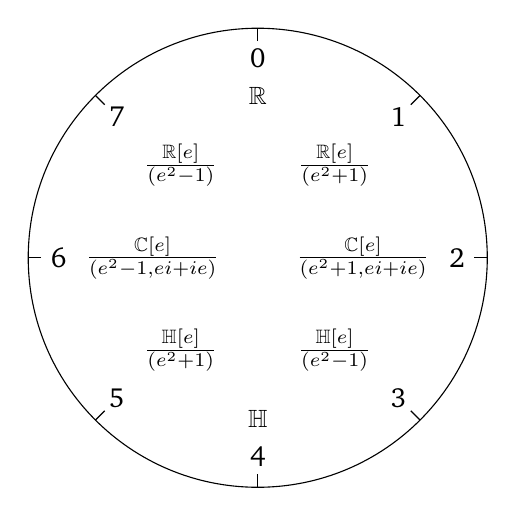
\begin{tikzpicture}[scale=1.1]
    \draw (0,0) circle[radius=2.65cm];
    \node[label=below:{\small$\mathbb{R}$}] at (90:2.3) {0};
    \node[label=below left:{$\frac{\mathbb{R}[e]}{(e^2+1)}$}] at (45:2.3) {1};
    \node[label=left:{$\frac{\mathbb{C}[e]}{(e^2+1,ei+ie)}$}] at (0:2.3) {2};
    \node[label=above left:{$\frac{\mathbb{H}[e]}{(e^2-1)}$}] at (-45:2.3) {3};
    \node[label=above:{\small$\mathbb{H}$}] at (-90:2.3) {4};
    \node[label=above right:{$\frac{\mathbb{H}[e]}{(e^2+1)}$}] at (-135:2.3) {5};
    \node[label=right:{$\frac{\mathbb{C}[e]}{(e^2-1,ei+ie)}$}] at (180:2.3) {6};
    \node[label=below right:{$\frac{\mathbb{R}[e]}{(e^2-1)}$}] at (135:2.3) {7};
    \foreach \a in {0,45,90,135,180,-135,-90,-45}
      \draw (\a:2.5) to (\a:2.65);
  \end{tikzpicture}
\] What does this notation mean? Well, as usual \(\mathbb{R}\),
\(\mathbb{C}\), and \(\mathbb{H}\) stand for the reals, complex numbers,
and quaternions. In all but two cases, we start with one of those
algebras and throw in an odd element ``\(e\)'' satisfying the relations
listed: \(e\) is either a square root of \(+1\) or of \(-1\), and in the
complex cases it anticommutes with \(i\).

So, for example, super division algebra number 1:
\[\mathbb{R}[e]/(e^2 + 1)\] is just the real numbers with an odd element
thrown in that satisfies \(e^2 + 1 = 0\). In other words, it's just the
complex numbers made into a superalgebra in such a way that \(i\) is
\emph{odd}.

The real reason I've arranged these guys in a circle numbered from 0 to
7 is to remind you of the Clifford algebra clock in
\protect\hyperlink{week210}{``Week 210''}, where I discussed the super
Brauer group of the real numbers, and said it was \(\mathbb{Z}/8\).

Indeed, the central super division algebras are a complete set of
representatives for this super Brauer group! In particular, the Clifford
algebra \(C_n\) is super Morita equivalent to the \(n\)th algebra on
this circle:

\begin{longtable}[]{@{}lll@{}}
\toprule
\(n\) & \(C_n\) & super-Morita-equivalent algebra\tabularnewline
\midrule
\endhead
\(0\) & \(\mathbb{R}\) & \(\mathbb{R}\)\tabularnewline
\(1\) & \(\mathbb{C}\) & \(\mathbb{R}[e]/(e^2+1)\)\tabularnewline
\(2\) & \(\mathbb{H}\) & \(\mathbb{C}[e]/(e^2+1,ei+ie)\)\tabularnewline
\(3\) & \(\mathbb{H}\oplus\mathbb{H}\) &
\(\mathbb{H}[e]/(e^2-1)\)\tabularnewline
\(4\) & \(\mathbb{H}(2)\) & \(\mathbb{H}\)\tabularnewline
\(5\) & \(\mathbb{C}(4)\) & \(\mathbb{H}[e]/(e^2+1)\)\tabularnewline
\(6\) & \(\mathbb{R}(8)\) &
\(\mathbb{C}[e]/(e^2-1,ei+ie)\)\tabularnewline
\(7\) & \(\mathbb{R}(8)\oplus\mathbb{R}(8)\) &
\(\mathbb{R}[e]/(e^2-1)\)\tabularnewline
\bottomrule
\end{longtable}

where the notation for Clifford algebras was explained last week.

I think this is cool. I'm not quite sure what to do with it yet, though.
How much of what people ordinarily do with division algebras can be done
with super division algebras? For example, can we define projective
spaces over super division algebras? (See
\protect\hyperlink{week106}{``Week 106''} and
\protect\hyperlink{week145}{``Week 145''} for why that would be
interesting.)

To read more about this, try:

\begin{enumerate}
\def\labelenumi{\arabic{enumi})}
\tightlist
\item
  Pierre Deligne, ``Notes on spinors'', in \emph{Quantum Fields and
  Strings: A Course For Mathematicians}, volume \textbf{1}, American
  Mathematical Society, Providence, 1999. Also available at
  \texttt{http://www.math.ias.edu/QFT/fall/spinors.ps}
\end{enumerate}

A lot of the ideas go back to here:

\begin{enumerate}
\def\labelenumi{\arabic{enumi})}
\setcounter{enumi}{1}
\tightlist
\item
  C. T. C. Wall, ``Graded Brauer groups'', \emph{J. Reine Angew. Math.}
  \textbf{213} (1963/1964), 187--199.
\end{enumerate}

and here's another good reference:

\begin{enumerate}
\def\labelenumi{\arabic{enumi})}
\setcounter{enumi}{2}
\tightlist
\item
  Peter Donovan and Max Karoubi, ``Graded Brauer groups and K-theory
  with local coefficients'', \emph{Publications Math. IHES} \textbf{38}
  (1970), 5--25. Also available at
  \texttt{http://www.math.jussieu.fr/\textasciitilde{}karoubi/Donavan.K.pdf}
\end{enumerate}

I should admit that I have a yearning to classify \emph{nonassociative}
super division algebras. Has anyone ever tried this? It's already plain
to see that we have two \(16\)-dimensional nonassociative super division
algebras: \[\mathbb{O}[e]/(e^2 + 1)\] and \[\mathbb{O}[e]/(e^2 - 1)\]
where \(e\) is an odd element that commutes with all the octonions. (I
should have mentioned this before, when talking about \(\mathbb{H}[e]\):
even though the quaternions are noncommutative, we assume that \(e\)
commutes with all of them.) Maybe one of these algebras deserves to be
called the \emph{superoctonions}. I bet these or something awfully
similar are lurking around in string theory.

Hmm\ldots{} next I wanted to write something about the topology of Bott
periodicity and how \emph{that} fits into what I've been discussing, but
I'm running out of energy. Let me say it briefly, without much detail,
just in case I never get around to a decent explanation.

Two super algebras are super Morita equivalent precisely when they have
equivalent categories of super representations. So, the super Brauer
group really consists of 8 different \emph{categories}: the categories
\(\mathsf{SuperRep}(C_n)\), where Bott periodicity says
\[\mathsf{SuperRep}(C_{n+8}) \sim \mathsf{SuperRep}(C_n)\] Moreover
these are symmetric monoidal categories, since direct summing lets us
``add'' objects in these categories in a nice way.

A long time ago, Graeme Segal figured out how to take a symmetric
monoidal category and get an infinite loop space from it. I explained
this construction in \protect\hyperlink{week199}{``Week 199''}, but for
a much more detailed and intense treatment with lots of references to
earlier work, try:

\begin{enumerate}
\def\labelenumi{\arabic{enumi})}
\setcounter{enumi}{3}
\tightlist
\item
  R. W. Thomason, ``Symmetric categories model all connective spectra'',
  \emph{Theory and Applications of Categories} \textbf{1} (1995),
  78--118. Available at
  \texttt{http://www.tac.mta.ca/tac/volumes/1995/n5/1-05abs.html}
\end{enumerate}

If we do this to \(\mathsf{SuperRep}(C_n)\), I think we get something
like \[\Omega^n(kO)\] that is, the \(n\)-fold loop space of something
called \(kO\), the ``connective K-theory spectrum'', which I explained
in \protect\hyperlink{week105}{``Week 105''}. The fact that this repeats
with period 8: \[\Omega^{n+8}(kO) \sim \Omega^n(kO)\] is the topological
version of Bott periodicity --- see \protect\hyperlink{week105}{``Week
105''} for more. So, we get the topological version of Bott periodicity
from the algebraic version by turning symmetric monoidal categories into
infinite loop spaces!

But, the interesting puzzle here is: what process can we do to
\(\mathsf{SuperRep}(C_n)\) to get \(\mathsf{SuperRep}(C_{n+1})\), which
is the algebraic version of looping? And I think the answer is: ``taking
super representations of \(C_1\) in it''. You see,
\[C_1 \otimes C_n = C_{n+1}\] where I'm using the super tensor product
of superalgebras, and this means that the category of representations of
\(C_1\) in \(\mathsf{SuperRep}(C_n)\) is \(\mathsf{SuperRep}(C_{n+1})\).

And, if I were trying to really explain this instead of merely
scribbling notes about it, I would try to explain why this is because
\(C_1\) is the complex numbers, and the unit circle in the complex
numbers is related to \emph{loops}.

But, sigh, that will have to wait.

One more thing before I quit for today\ldots{}

I just saw a cool paper by Dror Bar-Natan, Thang Le and Dylan Thurston
about the ``Duflo isomorphism''. This is a cousin of the
Poincare-Birkhoff-Witt theorem, which in its best form says that the
universal enveloping algebra \(UL\) of a Lie algebra \(L\) is isomorphic
\emph{as a coalgebra} to the symmetric algebra \(SL\). You'll often see
worse versions of the PBW theorem in textbooks, and ugly proofs, but
James Dolan showed me the nice version and proof a while back.

The kernel of the idea is this: if \(L\) is the Lie algebra of a group
\(G\), \(UL\) consists of left-invariant differential operators on
\(G\), and there's a map \(UL \to SL\) sending any differential operator
to its ``symbol''. This is an isomorphism of vector spaces and even of
coalgebras, but not of algebras.

Anyway, there's something vaguely similar relating the invariant
subalgebras of \(UL\) and \(SL\). By ``invariant'' here, I mean that
since \(L\) acts as derivations of \(UL\) and \(SL\), we can look at the
subalgebra of either one consisting of guys who are killed by these
derivations; such guys are called ``invariant''. Physicists call
invariant elements of \(UL\) ``Casimirs'', after the first physicist to
think about this stuff. They commute with everything else in \(UL\).
Invariant elements of \(SL\) are like classical Casimirs: there's a
Poisson bracket on \(SL\), and these are the guys whose Poisson bracket
with everyone vanishes.

The Duflo map is an \emph{algebra isomorphism} from the invariant
subalgebra of \(SL\) to the invariant subalgebra of \(UL\). So, it's
like a very nice way to quantize Casimirs, one that gets along with
multiplication. It's called the ``Duflo map'' because it was invented by
Harish-Chandra for semisimple Lie algebras and for Kirillov in general.
Kirillov conjectured that it was always an isomorphism; what Duflo did
is prove it:

\begin{enumerate}
\def\labelenumi{\arabic{enumi})}
\setcounter{enumi}{4}
\tightlist
\item
  Michel Duflo, ``Operateurs differentiels bi-invariants sur un groupe
  de Lie'', \emph{Ann. Sci. Ecole Norm. Sup.} \textbf{10} (1977),
  265--288.
\end{enumerate}

Apparently all known proofs are sort of hard! According to Bar-Natan, Le
and Thurston:

\begin{quote}
In the book of Dixmier, the proof is given only in the last chapter and
it utilizes most of the results developed in the whole book, including
many classification results (a situation Godement called
``scandalous''). As discussed below, there have been several recent
proofs that do not use classification results, but they all use tools
from well outside the natural domain of the problem.
\end{quote}

The proof by Bar-Natan, Le and Thurston uses the connection between knot
theory and Lie algebras --- namely, the theory of Vassiliev invariants.
I think there's still something slightly scandalous about this, but it's
awfully interesting. Anyway, take a look:

\begin{enumerate}
\def\labelenumi{\arabic{enumi})}
\setcounter{enumi}{5}
\tightlist
\item
  Dror Bar-Natan, Thang T. Q. Le and Dylan P. Thurston, ``Two
  applications of elementary knot theory to Lie algebras and Vassiliev
  invariants'', \emph{Geometry and Topology} \textbf{7} (2003), 1--31.
  Available at
  \texttt{http://www.maths.warwick.ac.uk/gt/GTVol7/paper1.abs.html} and
  also as
  \href{http://www.arXiv.org/abs/math.QG/0204311}{\texttt{math.QG/0204311}}.
\end{enumerate}

For more, try Thurston's thesis:

\begin{enumerate}
\def\labelenumi{\arabic{enumi})}
\setcounter{enumi}{6}
\tightlist
\item
  Dylan P. Thurston, ``Wheeling: a diagrammatic analogue of the Duflo
  isomorphism'',
  \href{http://www.arXiv.org/abs/math.QG/0006083}{\texttt{math.QG/0006083}}.
\end{enumerate}

and, just for fun, Deligne's handwritten letter to Bar-Natan:

\begin{enumerate}
\def\labelenumi{\arabic{enumi})}
\setcounter{enumi}{7}
\tightlist
\item
  Pierre Deligne, letter to Dror Bar-Natan about the Duflo map,
  available at
  \texttt{http://www.math.toronto.edu/\textasciitilde{}drorbn/Deligne/}
\end{enumerate}

\begin{center}\rule{0.5\linewidth}{0.5pt}\end{center}

\textbf{Addendum:} Todd Trimble has kindly allowed me to append some
rough notes in which he outlines proofs of some results above.

\begin{quote}
From: Todd Trimble Subject: notes on super Brauer To: John Baez Cc:
James Dolan Date: Sun, 27 Mar 2005 19:30:00 -0500

John,

These are some notes on some of the super Brauer discussion.

\begin{enumerate}
\def\labelenumi{\arabic{enumi}.}
\tightlist
\item
  Let \(V\) be the category of finite-dimensional super vector spaces
  over \(\mathbb{R}\). By super algebra I mean a monoid in this
  category. There's a bicategory whose objects are super algebras \(A\),
  whose 1-cells \(M\colon A \to B\) are left \(A\)- right \(B\)-modules
  in \(V\), and whose 2-cells are homomorphisms between modules. This is
  a symmetric monoidal bicategory under the usual tensor product on
  \(V\).
\end{enumerate}

\(A\) and \(B\) are super Morita equivalent if they are equivalent
objects in this bicategory. Equivalence classes \([A]\) form an abelian
monoid whose multiplication is given by the monoidal product. The super
Brauer group of \(\mathbb{R}\) is the subgroup of invertible elements of
this monoid.

If \([B]\) is inverse to \([A]\) in this monoid, then in particular
\(A \otimes (-)\) can be considered left biadjoint to \(B \otimes (-)\).
On the other hand, in the bicategory above we always have a biadjunction
\[\frac{A\otimes C\to D}{C\to A^*\otimes D}\] (essentially because left
\(A\)-modules are the same as right \(A^*\)-modules, where \(A^*\)
denotes the super algebra opposite to \(A\)). Since right biadjoints are
unique up to equivalence, we see that if an inverse to \([A]\) exists,
it must be \([A^*]\).

This can be sharpened: an inverse to \([A]\) exists iff the unit and
counit \[1\to A^*\otimes A \qquad A\otimes A^*\to 1\] are equivalences
in the bicategory. Actually, one is an equivalence iff the other is,
because both of these canonical 1-cells are given by the same
\(A\)-bimodule,\\
namely the one given by \(A\) acting on both sides of the underlying
superspace of \(A\) (call it \(S\)) by multiplication.\\
Either is an equivalence if the bimodule structure map
\[A^* \otimes A \to \mathrm{Hom}(S, S),\] which is a map of super
algebras, is an isomorphism.

\begin{enumerate}
\def\labelenumi{\arabic{enumi}.}
\setcounter{enumi}{1}
\tightlist
\item
  As an example, let \(A = C_1\) be the Clifford algebra generated by
  the \(1\)-dimensional space \(\mathbb{R}\) with the usual quadratic
  form \(Q(x) = |x|^2\), and \(\mathbb{Z}/2\)-graded in the usual way.
  Thus, the homogeneous parts of \(A\) are \(1\)-dimensional and there
  is an odd generator \(i\) satisfying \(i^2 = -1\). The opposite
  \(A^*\) is similar except that there is an odd generator \(e\)
  satisfying \(e^2 = 1\). Under the map
  \[A^* \otimes A \to \mathrm{Hom}(S, S),\] where we write \(S\) as a
  sum of even and odd parts \(R + Ri\), this map has a matrix
  representation \[
    \begin{aligned}
  e\otimes i
  &\mapsto
  \left(\begin{array}{cc}-1&0\\0&1\end{array}\right)
    \\1\otimes i
  &\mapsto
  \left(\begin{array}{cc}0&-1\\1&0\end{array}\right)
    \\e\otimes 1
  &\mapsto
  \left(\begin{array}{cc}0&1\\1&0\end{array}\right)
    \end{aligned}
  \] which makes it clear that this map is surjective and thus an
  isomorphism. Hence \([C1]\) is invertible.
\end{enumerate}

One manifestation of Bott periodicity is that \([C1]\) has order 8. We
will soon see a very easy proof of this fact. A theorem of C.T.C. Wall
is that \([C1]\) in fact generates the super Brauer group; I believe
this can be shown by classifying super division algebras, as discussed
below.

\begin{enumerate}
\def\labelenumi{\arabic{enumi}.}
\setcounter{enumi}{2}
\tightlist
\item
  That \([C1]\) has order 8 is an easy calculation. Let \(C_r\) denote
  the \(r\)-fold tensor of \(C_1\). \(C_2\) for instance has two
  super-commuting odd elements \(i\), \(j\) satisfying
  \(i^2 = j^2 = -1\); it follows that \(k := ij\) satisfies\\
  \(k^2 = -1\), and we get the usual quaternions, graded so that the
  even part is the span \(\langle 1, k\rangle\) and the odd part is
  \(\langle i, j\rangle\).
\end{enumerate}

\(C_3\) has three super-commuting odd elements \(i\), \(j\), \(l\), all
of which are square roots of \(-1\). It follows that \(e = ijl\) is an
odd central involution (here ``central'' is taken in the ungraded
sense), and also that \(i' = jl\), \(j' = li\), \(k' = ij\) satisfy the
Hamiltonian equations \[(i')^2 = (j')^2 = (k')^2 = i'j'k' = -1,\] so we
have \(C_3 = \mathbb{H}[e]/(e2 - 1)\). Note this is the same as
\[\mathbb{H} \otimes (C_1)^*\] where the \(\mathbb{H}\) here is the
quaternions viewed as a super algebra concentrated in degree 0 (i.e.~is
purely bosonic).

Then we see immediately that \(C_4 = C_3 \otimes C_1\) is equivalent to
purely bosonic \(\mathbb{H}\) (since the \(C_1\) cancels \((C_1)^*\) in
the super Brauer group).

At this point we are done: we know that conjugation on (purely bosonic)
\(\mathbb{H}\) gives an isomorphism \[\mathbb{H}^* \to \mathbb{H}\]
hence \([\mathbb{H}]-1 = [\mathbb{H}^*] = [\mathbb{H}]\),
i.e.~\([\mathbb{H}] = [C4]\) has order 2!\\
Hence \([C1]\) has order 8.

\begin{enumerate}
\def\labelenumi{\arabic{enumi}.}
\setcounter{enumi}{3}
\tightlist
\item
  All this generalizes to Clifford algebras: if a real quadratic vector
  space \((V, Q)\) has signature \((r, s)\), then the super algebra
  \(\mathrm{Cliff}(V, Q)\) is isomorphic to \(A_r \otimes (A^*)_s\),
  where \(A_r\) denotes \(r\)-fold tensor product of \(A = C_1\). By the
  above calculation we see that \(\mathrm{Cliff}(V, Q)\) is equivalent
  to \(C_{r-s}\) where \(r-s\) is taken modulo 8.
\end{enumerate}

For the record, then, here are the hours of the super Clifford clock,
where \(e\) denotes an odd element, and \(\sim\) denotes equivalence:

\begin{itemize}
\tightlist
\item
  \(C_0 \sim \mathbb{R}\)
\item
  \(C_1 \sim \mathbb{R}\oplus\mathbb{R}[e]\), \(e2 = -1\)
\item
  \(C_2 \sim \mathbb{C}\oplus\mathbb{C}[e]\), \(e2 = -1, ei = -ie\)
\item
  \(C_3 \sim \mathbb{H}\oplus\mathbb{H}[e]\),
  \(e2 = 1, ei = ie, ej = je, ek = ke\)
\item
  \(C_4 \sim \mathbb{H}\)
\item
  \(C_5 \sim \mathbb{H}\oplus\mathbb{H}[e]\),
  \(e2 = -1, ei = ie, ej = je, ek = ke\)
\item
  \(C_6 \sim \mathbb{C}\oplus\mathbb{C}[e]\), \(e2 = 1, ei = -ie\)
\item
  \(C_7 \sim \mathbb{R}\oplus\mathbb{R}[e]\), \(e2 = 1\)
\end{itemize}

All the super algebras on the right are in fact super division algebras,
i.e.~super algebras in which every nonzero homogeneous element is
invertible.

To prove Wall's result that \([C1]\) generates the super Brauer group,
we need a lemma: any element in the super Brauer group is the class of a
super division algebra.

{[}To be continued. I had wanted to show that every element in the super
Brauer group must be of the form \([A]\) where \(A\) is a super division
algebra, and then classify super (associative) division algebras,
showing on a case by case basis that those not in the super Clifford
clock above are seen not to belong to the super Brauer group.{]}

Todd
\end{quote}

Todd finished off the job later\ldots{} though by this point we had
formulated the grander goal of classifying not-necessarily-associative
super division algebras!

\begin{quote}
From: Todd Trimble Subject: super division algebras To: John Baez Date:
Wed, 27 Apr 2005 22:17:12 EDT

John,

This is a warm-up to classifying super division algebras over
\(\mathbb{R}\), where I'll consider just the associative case.\\
Nothing I say will be deep, but I found it somewhat fun and diverting,
and there may be echoes of things to come.

I'll take as known that the only associative division algebras over
\(\mathbb{R}\) are \(\mathbb{R}\), \(\mathbb{C}\), \(\mathbb{H}\) -- the
even part \(A\) of an associative super division algebra must be one of
these cases. We can express the associativity of a super algebra (with
even part \(A\)) by saying that the odd part \(M\) is an \(A\)-bimodule
equipped with a \(A\)-bimodule map pairing
\[\langle -,-\rangle \colon M\otimes_A M \to A\] such that:
\[a\langle b,c\rangle = \langle a,b\rangle c \quad \mbox{for all $a,b,c$ in $M$.} \tag{$\star\star$}\]

If the super algebra is a super division algebra which is not wholly
concentrated in even degree, then multiplication by a nonzero odd
element induces an isomorphism \[A \to M\] and so \(M\) is
\(1\)-dimensional over \(A\); choose a basis element \(e\) for \(M\).

The key observation is that for any \(a\) in \(A\), there exists a
unique \(a'\) in \(A\) such that \[ae = ea'\] and that the
\(A\)-bimodule structure forces \((ab)' = a'b'\). Hence we have an
automorphism (fixing the real field) \[(--)'\colon A \to A\] and we can
easily enumerate (up to isomorphism) the possibilities for associative
super division algebras over \(\mathbb{R}\):

\begin{enumerate}
\def\labelenumi{\arabic{enumi}.}
\item
  \(A = \mathbb{R}\). Here we can adjust \(e\) so that either
  \(e^2 := \langle e, e\rangle\) is \(-1\) or \(1\). The corresponding
  super division algebras occur at 1 o'clock and 7 o'clock on the super
  Brauer clock.
\item
  \(A = \mathbb{C}\). There are two \(\mathbb{R}\)-automorphisms
  \(\mathbb{C} \to \mathbb{C}\). In the case where the automorphism is
  conjugation, condition (\(\star\star\)) for super associativity gives
  \(\langle e, e\rangle e = e\langle e, e\rangle\) so that
  \(\langle e, e\rangle\) must be real. Again \(e\) can be adjusted so
  that \(\langle e, e\rangle\) is \(-1\) or \(1\). These possibilities
  occur at 2 o'clock and 6 o'clock on the super Brauer clock.
\end{enumerate}

For the identity automorphism, we can adjust \(e\) so that
\(\langle e, e\rangle\) is \(1\). This gives the super algebra
\(\mathbb{C}[e]/(e^2 - 1)\) (where \(e\) commutes with elements in
\(\mathbb{C}\)). This does not occur on the super Brauer clock over
\(\mathbb{R}\). However, it does generate the super Brauer group over
\(\mathbb{C}\) (which is of order two).

\begin{enumerate}
\def\labelenumi{\arabic{enumi}.}
\setcounter{enumi}{2}
\tightlist
\item
  \(A = \mathbb{H}\). Here \(\mathbb{R}\)-automorphisms
  \(\mathbb{H} \to \mathbb{H}\) are given by \(h \mapsto xhx^{-1}\) for
  \(x\) in \(\mathbb{H}\). In other words \[he = exhx^{-1}\] whence
  \(ex\) commutes with all elements of \(\mathbb{H}\) (i.e.~we can
  assume wlog that the automorphism is the identity). The properties of
  the pairing guarantee that
  \(h\langle e, e\rangle = \langle e, e\rangle h\) for all \(h\) in
  \(\mathbb{H}\), so \(\langle e, e\rangle\) is real and again we can
  adjust \(e\) so that \(\langle e, e\rangle\) is \(1\) or \(-1\). These
  cases occur at 3 o'clock and 5 o'clock on the super Brauer clock.
\end{enumerate}

This appears to be a complete (even if a bit pedestrian) analysis.

Best,

Todd
\end{quote}

\begin{center}\rule{0.5\linewidth}{0.5pt}\end{center}



\hypertarget{week213}{%
\section{April 3, 2005}\label{week213}}

Here's a book I've been reading lately:

\begin{enumerate}
\def\labelenumi{\arabic{enumi})}
\tightlist
\item
  Kenneth S. Brown, \emph{Cohomology of Groups}, Graduate Texts in
  Mathematics \textbf{182}, Springer, 1982.
\end{enumerate}

I should have read this book a long time ago --- but I probably wouldn't
have enjoyed it as much as I do now. All sorts of things I struggled to
learn for years are neatly laid out here. Best of all, he comes right
out and admits from the start that the cohomology of groups is really a
branch of \emph{topology}, instead of hiding this fact like some people
do.

This is something every mathematician should know: you can take any
group and turn it into a space, thus ``reducing'' group theory to
topology. In particular, if you have any trick for telling spaces apart,
like ``cohomology theory'', you can apply it to groups as well.

Of course topology is \emph{harder} than group theory in many ways ---
hence my quotes around ``reducing''. Indeed, algebraic topology was
invented as a trick for reducing topology to group theory! But, the
bridge turns out to go both ways, and there's a lot of profitable
traffic in both directions.

Ultimately, as James Dolan likes to point out, it's all about the unity
of mathematics. Topology is about our concept of \emph{space}, while
group theory is about our concept of \emph{symmetry}\ldots{} but the
amazing fact is that they turn out to be two aspects of the same big
thing! Mathematics is a source of endless surprises, but this is one of
the biggest jaw-droppers of all.

The idea goes back at least to Evariste Galois, who noticed that you can
classify the ways a little thing can sit in a bigger thing by keeping
track of what we now call its ``Galois group'': the group of all
symmetries of the big thing that map the little thing to itself. For
example, you can pick out a point or line in the plane by keeping track
of which symmetries of the plane map this point or line to itself.

However, the idea of using groups to classify how a little thing sits in
a big one was really made explicit in Felix Klein's ``Erlangen
program'', a plan for reducing \emph{geometry} to group theory.

You may know Klein for his famous one-sided bottle:

\begin{quote}
A mathematician named Klein\\
Thought the Möbius strip was divine.\\
Said he: ``If you glue\\
The edges of two\\
You'll get a weird bottle like mine!''\\
\end{quote}

Or maybe you know that the symmetry group of a rectangle, including
reflections, is called the ``Klein 4-group'':

\begin{longtable}[]{@{}lcccc@{}}
\toprule
\(\cdot\) & \(1\) & \(a\) & \(b\) & \(c\)\tabularnewline
\midrule
\endhead
\(1\) & \(1\) & \(a\) & \(b\) & \(c\)\tabularnewline
\(a\) & \(a\) & \(1\) & \(c\) & \(b\)\tabularnewline
\(b\) & \(b\) & \(c\) & \(1\) & \(a\)\tabularnewline
\(c\) & \(c\) & \(b\) & \(a\) & \(1\)\tabularnewline
\bottomrule
\end{longtable}

He is also known for some other groups called ``Kleinian groups'', which
act as symmetries of fractal patterns like this:
\[\href{http://www.josleys.com/showpic.php?file=INDRA065.jpg&title=Indra20}{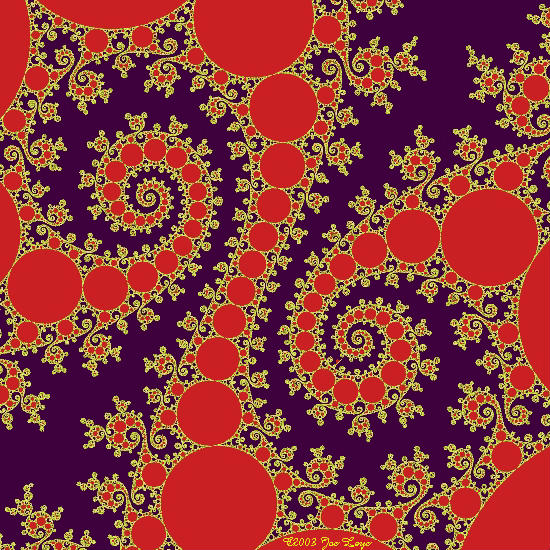
\includegraphics[max width=\linewidth]{../images/INDRA065.jpg}}\]

\begin{enumerate}
\def\labelenumi{\arabic{enumi})}
\setcounter{enumi}{1}
\tightlist
\item
  Jos Leys, ``Kleinian Pages'',
  \texttt{http://www.josleys.com/creatures42.htm}
\end{enumerate}

If you like cool pictures, check out this website! I've linked you to
the page that most closely connects to Kleinian groups, but there are
lots of other more fanciful pictures. And if you get interested in the
math lurking behind these fractals, you've \emph{got} to try this book:

\begin{enumerate}
\def\labelenumi{\arabic{enumi})}
\setcounter{enumi}{2}
\tightlist
\item
  David Mumford, Caroline Series, and David Wright, \emph{Indra's
  Pearls: The Vision of Felix Klein}, Cambridge U. Press, Cambridge,
  2002.
\end{enumerate}

Mumford is a world-class mathematician, so this book is completely
different from the superficial descriptions of fractals one often sees
in math popularizations --- but it's still readable, and it's packed
with beautiful pictures. You can learn a lot about Kleinian groups from
this!

The Kleinian groups arose from Klein's studies of complex functions,
which he considered his best work. But, he was also a mathematical
physicist. Among other things, he wrote a four-volume book on tops with
one of the fathers of quantum mechanics, Arnold Sommerfeld:

\begin{enumerate}
\def\labelenumi{\arabic{enumi})}
\setcounter{enumi}{3}
\tightlist
\item
  Felix Klein and Arnold Sommerfeld, \emph{Über die Theorie des
  Kreisels}, 4 vols, 1897--1910. Reprinted by Johnson, New York, 1965.
  Also available at
  \texttt{http://www.hti.umich.edu/cgi/t/text/text-idx?c=umhistmath;idno=ABV7354.0001.001}
\end{enumerate}

This came after a book he wrote on his own:

\begin{enumerate}
\def\labelenumi{\arabic{enumi})}
\setcounter{enumi}{4}
\tightlist
\item
  Felix Klein, \emph{The Mathematical Theory of the Top}, Scribner's,
  New York, 1887.
\end{enumerate}

This may seem like a lot of books about a kid's toy! But, tops are
profoundly related to the rotation group, and the ``exactly solvable''
tops discovered by Euler, Lagrange/Poisson, and Sofia Kowalevskaya are
solvable because of their symmetries --- deeply hidden symmetries, in
the case of the Kowalevskaya top. So, one can imagine why Klein liked
this subject.

Klein also wrote a book on the icosahedron and the quintic equation:

\begin{enumerate}
\def\labelenumi{\arabic{enumi})}
\setcounter{enumi}{5}
\tightlist
\item
  Felix Klein, \emph{Lectures on the Icosahedron and the Solution of
  Equations of the Fifth Degree}, 1888. Reprinted by Dover, New York,
  2003. Also available at
  \texttt{http://historical.library.cornell.edu/cgi-bin/cul.math/docviewer?did=03070001\&seq=7}
\end{enumerate}

Galois had already noticed that the number field you get by taking the
rationals and throwing in the roots of a typical quintic:
\[ax^5 + bx^4 + cx^3 + dx^2 + ex + f = 0\] has as its symmetry group all
the permutations of the 5 roots. Indeed, he saw that the
``unsolvability'' of this group, in a technical sense, is what makes it
impossible to solve the quintic by radicals. It must have been common
knowledge that the symmetry group of the icosahedron is the group of all
\emph{even} permutations of 5 things. But, Klein took this much further!
Alas, I've never really understood what he did. Perhaps if I read these
and think hard, I'll understand:

\begin{enumerate}
\def\labelenumi{\arabic{enumi})}
\setcounter{enumi}{6}
\item
  Jerry Shurman, \emph{Geometry of the Quintic}, John Wiley and Sons,
  New York, 1997.

  Peter Doyle and Curt McMullen, ``Solving the quintic by iteration'',
  \emph{Acta Math.} \textbf{163} (1989), 151--180. Available at
  \texttt{http://math.dartmouth.edu/\textasciitilde{}doyle/docs/icos/icos/icos.html}
\end{enumerate}

Anyway, it should be clear by now that Klein was a lover of symmetry. He
was also a bit of a visionary, and his obituary by Grace Chisholm Young
shows that this got him in some trouble:

\begin{quote}
One of Weierstrass' pupils, still alive, told me that at Berlin Klein
was anathema: it was said that his work was not mathematics at all, but
mere talk. This criticism shows a want of appreciation of his rare type
of mind. It teemed with ideas and brilliant reflections, but it is true
that his work lacks the stern aspects required by mathematical
exactitude. It was in personal contact that this was corrected, at least
in so far as his students were concerned. His favourite maxim was,
``Never be dull''.
\end{quote}

In a talk he wrote in 1872 when he was made professor at Erlangen
University --- a talk he didn't actually give! --- Klein outlined what
is now called his ``Erlangen program''. The idea here is that different
kinds of geometry correspond to different symmetry groups. Taken to the
extreme, this philosophy says that a geometry is just a group! In a
given geometry, a ``figure'' of any kind --- like a point or line ---
can be detected by the subgroup of symmetries that map that figure to
itself. So, a figure is just a subgroup!

This program eventually led to a grand theory of groups and geometry
based on ``flag manifolds'', which I tried to sketch in
\protect\hyperlink{week178}{``Week 178''},
\protect\hyperlink{week180}{``Week 180''}, and
\protect\hyperlink{week181}{``Week 181''}.

It's important to realize how similar the Erlangen program is to Galois
theory. Galois had also used group theory to classify how a little thing
can sit in a bigger thing, but in situations where the ``things'' in
question are commutative algebras --- for example, the rational numbers
with some roots of polynomials thrown in.

Now, commutative algebra is like topology, only backwards. Any space has
a commutative algebra consisting of functions on it, and if we're very
clever we can think of any commutative algebra as functions on some
space --- though this was only achieved long after Galois, by Alexander
Grothendieck.

What do I mean by ``backwards''? Well, suppose you have a ``covering
space'' --- a big space sitting over a little one, like a spiral sitting
over the circle. In this situation, any function on the little space
downstairs defines a function on the big one upstairs. So, the algebra
of functions on the little space sits inside the algebra of functions on
the big space.

Notice how it's backwards. Classifying how a little commutative algebra
can sit in a big one amounts to classifying how a big space can cover a
little one! For more details on this analogy, try
\protect\hyperlink{week198}{``Week 198''},
\protect\hyperlink{week201}{``Week 201''} and especially
\protect\hyperlink{week205}{``Week 205''}.

I should warn you: the Galois group has a different name when we apply
it to the classification of covering spaces --- we call it the group of
``deck transformations''. The idea is pretty simple. Suppose \(Y\) is a
covering space of \(X\), like this: \[
  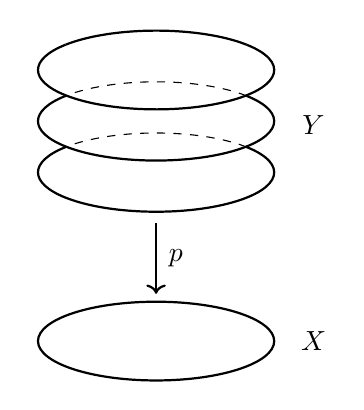
\begin{tikzpicture}
    \draw[thick] (0,0) ellipse (1.5cm and 0.5cm);
    \draw[thick] (40:1.5)++(0,1.5) arc (40:-220:1.5cm and 0.5cm);
    \draw[dashed] (40:1.5)++(0,1.5) arc (40:140:1.5cm and 0.5cm);
    \draw[thick] (40:1.5)++(0,2.15) arc (40:-220:1.5cm and 0.5cm);
    \draw[dashed] (40:1.5)++(0,2.15) arc (40:140:1.5cm and 0.5cm);
    \draw[thick] (40:1.5)++(0,2.8) arc (40:-220:1.5cm and 0.5cm);
    \draw[thick] (40:1.5)++(0,2.8) arc (40:140:1.5cm and 0.5cm);
    \draw[thick,->] (0,1.5) to node[label={[label distance=-1mm]right:{$p$}}]{} (0,0.6);
    \node at (2,0) {$X$};
    \node at (2,2.75) {$Y$};
  \end{tikzpicture}
\] We've got a function \(p\colon Y \to X\), and sitting over each point
of \(X\) are the same number of points of \(Y\), living on different
``sheets'' that look locally just like \(X\). You should imagine the
sheets being able to twist around from place to place, like the edges of
a Moebius strip.

Anyway, a ``deck transformation'' is just a way of mapping \(Y\) to
itself that permutes the different points sitting over each point of
\(X\).

The theory of this was worked out by Riemann, Poincare, and others.
Poincare showed you could use this idea to turn any connected space
\(X\) into a group --- its ``fundamental group''. There are different
ways to define this, but one is to form the most complicated possible
covering space of \(X\) that's still connected --- its ``universal
cover''. Then, take the group of deck transformations of this! Following
Galois' philosophy, all the other connected covering spaces of \(X\)
correspond to subgroups of this group.

The theory of the fundamental group was just the beginning when it came
to groups and topology. One of many later big steps, back in the late
1940s, was due to Sammy Eilenberg and Saunders Mac Lane. They saw how to
reverse the ``fundamental group'' idea and turn any group back into a
space!

More precisely: for any group \(G\), there's a space whose fundamental
group is \(G\) and whose higher homotopy groups vanish. It's sometimes
called the ``Eilenberg--Mac Lane space'' and denoted \(K(G,1)\), but
sometimes it's called the ``classifying space'' and denoted \(BG\). It's
pretty easy to build; I described how back in
\protect\hyperlink{week70}{``Week 70''}.

You start with a point: \[\bullet\] Then you stick on an edge looping
from this point to itself for each element \(a\) in \(G\). Unrolled, it
looks like this: \[
  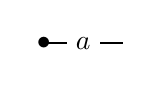
\begin{tikzpicture}
    \draw[thick] (0,0) node{$\bullet$} to node[fill=white]{$a$} (1,0);
  \end{tikzpicture}
\] where \(a\) is an element of our group. Then, whenever we have
\(ab = c\) in our group, we stick on a triangle like this: \[
  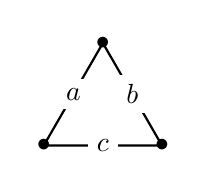
\begin{tikzpicture}
    \draw[thick] (0,0) node{$\bullet$} to node[fill=white]{$c$} (1.5,0) node{$\bullet$} to node[fill=white]{$b$} (0.75,1.3) node{$\bullet$} to node[fill=white]{$a$} cycle;
  \end{tikzpicture}
\] Then, whenever we have \(abc = d\) in our group, we stick on a
tetrahedron like this: \[
  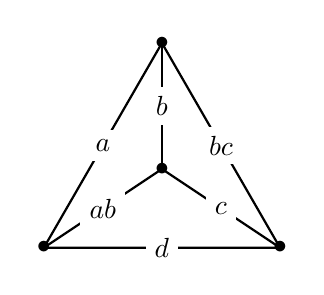
\begin{tikzpicture}
    \draw[thick] (0,0) node{$\bullet$} to node[fill=white]{$d$} (3,0) node{$\bullet$} to node[fill=white]{$bc$} (1.5,2.6) node{$\bullet$} to node[fill=white]{$a$} cycle;
    \draw[thick] (0,0) to node[fill=white]{$ab$} (1.5,1) node{$\bullet$};
    \draw[thick] (1.5,2.6) to node[fill=white]{$b$} (1.5,1);
    \draw[thick] (3,0) to node[fill=white]{$c$} (1.5,1);
  \end{tikzpicture}
\] And so on, forever! For each list of \(n\) group elements, we get an
\(n\)-dimensional simplex in our Eilenberg-Mac Lane space. The resulting
space knows everything about the group we started with. In particular,
the fundamental group of this space will be the group we started with!

Using this idea, we can do some fiendish things. For example, for each
\(n\) we can form a set \(C_n(G,A)\) consisting of all functions that
eat \(n\)-dimensional simplices in the Eilenberg-Mac Lane space of \(G\)
and spit out elements of some abelian group \(A\). There are maps
\[d\colon C_n(G,A) \to C_{n+1}(G,A)\] reflecting the fact that each
\((n+1)\)-simplex has a bunch of \(n\)-simplices as its faces. Since the
boundary of a boundary is zero, \[d^2 = 0\] Guys who live in the kernel
of \[d\colon C_n(G,A) \to C_{n+1}(G,A)\] are called ``\(n\)-cocycles'',
and guys who live in the image of \[d\colon C_{n-1}(G,A) \to C_n(G,A)\]
are called ``\(n\)-coboundaries''. Since \(d^2 = 0\), every coboundary
is a cocycle, but not always vice versa. So, we can form the group of
cocycles mod coboundaries. This is called the ``\(n\)th cohomology
group'' of \(G\) with coefficients in \(A\), and it's denoted
\[H^n(G,A)\] This sounds unmotivated at first, but the \(n\)th
cohomology group of a space is really just a clever way of keeping track
of \(n\)-dimensional holes in that space. So, what we're doing here is
cleverly defining a way to study ``holes'' in a \emph{group!} There are
deeper, more conceptual ways of understanding group cohomology, but this
is not bad for starters.

For example, let's take the simplest group that's not \emph{utterly}
dull --- the integers \(\mod 2\), or \(\mathbb{Z}/2\). Here we get
\[K(\mathbb{Z}/2,1) = \mathbb{RP}^\infty\] where \(\mathbb{RP}^\infty\)
is the space formed by taking an infinite-dimensional sphere and
identifying opposite points. This space has holes of arbitrarily high
dimension, so the cohomology groups of \(\mathbb{Z}/2\) go on being
nontrivial for arbitrarily high \(n\). I sketched a ``picture proof''
here:

\begin{enumerate}
\def\labelenumi{\arabic{enumi})}
\setcounter{enumi}{7}
\tightlist
\item
  John Baez, Fall 2004 Quantum Gravity Seminar, week 10, notes by Derek
  Wise, \texttt{http://math.ucr.edu/home/baez/qg-fall2004/}
\end{enumerate}

and I showed that, for example \[
  H_n(\mathbb{Z}/2,\mathbb{Z}) =
  \begin{cases}
    \mathbb{Z} &\mbox{if $n=0$;}
  \\0 &\mbox{if $n$ is odd;}
  \\\mathbb{Z}/2 &\mbox{if $n$ is even and non-zero.}
  \end{cases}
\] I also explained how this stuff is related to topological quantum
field theory.

Anyway, all this is just the very superficial beginnings of the subject
of group cohomology. Read Brown's book to dig deeper!

Personally, what I find most exciting about this book now are the
remarks on the ``Euler characteristic'' of a group. Let me explain
this\ldots{} though now I'll have to pull out the stops and assume you
know some group cohomology.

We can try to define the ``Euler characteristic'' of a group \(G\) to be
the Euler characteristic of \(K(G,1)\). This is the alternating sum of
the dimensions of the rational cohomology groups \[H_n(G,\mathbb{Q})\]
Of course, this alternating sum only converges if the cohomology groups
vanish for big enough \(n\). Also, they all need to be
finite-dimensional.

Unfortunately, not many groups have well-defined Euler characteristic
with this naive definition!

For example, people have studied groups \(G\) whose \(n\)th cohomology
vanishes for \(n > d\), regardless of the coefficients. If we take the
smallest \(d\) for which this holds, such a group \(G\) is said to have
``cohomological dimension'' \(d\). Eilenberg and Ganea showed that for
\(d \geqslant 3\), a group has cohomological dimension \(d\) whenever we
can build \(K(G,1)\) as a simplicial complex (or CW complex) with no
cells of dimension more than \(d\).

This is a nice geometrical interpretation of the cohomological
dimension. But, one can show that groups with torsion never have finite
cohomological dimension! We've seen an example already:
\(\mathbb{Z}/2\), whose Eilenberg-Mac Lane space is
infinite-dimensional.

However, it turns out that there's a generalization of the Euler
characteristic that makes sense for any group \(G\) that has a
torsion-free subgroup \(H\) whose Euler characteristic is well-defined
in the naive way, as long as \(H\) has finite index in \(G\). We just
define the Euler characteristic of \(G\) to be the Euler characteristic
of \(H\) divided by the index of \(H\) in \(G\). The answer doesn't
depend on the choice of \(H\)!

Take my favorite example, \(\mathrm{SL}(2,\mathbb{Z})\). This has
torsion, so its cohomological dimension is infinite and its naive Euler
characteristic is undefined! Indeed, I wrote a whole issue of This
Week's Finds about some elements of orders 4 and 6 sitting inside
\(\mathrm{SL}(2,\mathbb{Z})\), related to the symmetries of square and
hexagonal lattices --- see \protect\hyperlink{week125}{``Week 125''}.

But, \(\mathrm{SL}(2,\mathbb{Z})\) has a torsion-free subgroup of index
12, namely its commutator subgroup --- the group you need to quotient by
to make \(\mathrm{SL}(2,\mathbb{Z})\) be abelian. This subgroup has
finite cohomological dimension and its Euler characteristic is \(-1\).
I'm not sure why this is true, but Brown says so! This means the Euler
characteristic of \(\mathrm{SL}(2,\mathbb{Z})\) works out to be
\(-1/12\).

If you've read my stuff about Euler characteristics in
\protect\hyperlink{week147}{``Week 147''}, you'll see why this gets me
so excited --- I can add this stuff to my list of weird ways of
calculating the Euler characteristic. Plus, it's related to the magical
role of the number ``24'' in string theory, and also the Riemann zeta
function!

Indeed, the Riemann zeta function gives a way to make rigorous Euler's
zany observation that \[1 + 2 + 3 + \ldots = -\frac{1}{12},\] as I
explained here:

\begin{enumerate}
\def\labelenumi{\arabic{enumi})}
\setcounter{enumi}{8}
\tightlist
\item
  John Baez, ``Euler's Proof that \(1+2+3+\ldots=-1/12\), Bernoulli
  Numbers and the Riemann Zeta Function'', Winter 2004 Quantum Gravity
  Seminar, homework for weeks 5,6,7, available at
  \texttt{http://math.ucr.edu/home/baez/qg-winter2004/}
\end{enumerate}

This suggests that there should be a version of the Eilenberg-Mac Lane
space for \(\mathrm{SL}(2,\mathbb{Z})\) which has 1 cell of dimension
\(0\), 2 cells of dimension \(2\), 3 cells of dimension \(4\), and so
on. Does anyone know if this is true?

More generally, G. Harder computed the (generalized) Euler
characteristic for a large class of arithmetic groups:

\begin{enumerate}
\def\labelenumi{\arabic{enumi})}
\setcounter{enumi}{9}
\tightlist
\item
  G. Harder, ``A Gauss-Bonnet formula for discrete arithmetically
  defined groups'', \emph{Ann. Sci. Ecole Norm. Sup.} \textbf{4} (1971),
  409--455.
\end{enumerate}

For example, he looked at the symplectic group defined over the
integers, \(\mathrm{Sp}(n,\mathbb{Z})\), and showed that its Euler
characteristic is this product of values of the Riemann zeta function:
\[\zeta(-1) \zeta(-3) \cdots \zeta(1-2n)\] In the case \(n = 1\) we get
back \(\mathrm{SL}(2,\mathbb{Z})\) and \(\zeta(-1) = -1/12\).

In fact, every Chevalley group over the integers has a well-defined
Euler characteristic, and Harder was able to compute it in terms of
Bernoulli numbers. A Chevalley group is sort of like a simple Lie group,
but defined algebraically. \(\mathrm{Sp}(n,\mathbb{Z})\) is one example.
\(\mathrm{SL}(n,\mathbb{Z})\) is another, but it's Euler characteristic
turns out to vanish for \(n > 2\), so it's not too interesting.

Harder worked them all out. For example, he showed the Euler
characteristic of the integral form of the exceptional group
\(\mathrm{E}_7\) is some wacky number like
\[- \frac{691 \times 43867}{2^{21} \times 3^9 \times 5^2 \times 7^3 \times 11 \times 13 \times 19}\]
Serre went even further, computing Euler characteristics of Chevalley
groups defined over algebraic number fields. He also noticed that when
you write the Euler characteristic of a group as a fraction, the primes
in the denominator are precisely the primes \(p\) for which the group
has \(p\)-torsion. He was thus able to conclude, for example, that
\(\mathrm{E}_7\) defined over the integers has \(p\)-torsion for
\(p = 2, 3, 5, 7, 11, 13, 19\).

For more, see:

\begin{enumerate}
\def\labelenumi{\arabic{enumi})}
\setcounter{enumi}{10}
\tightlist
\item
  Jean-Pierre Serre, ``Cohomologie des groups discretes'', \emph{Ann.
  Math. Studies} \textbf{70} (1971), 77--169.
\end{enumerate}

This only takes us up to 1971. I shudder to think what bizarre results
along these lines are known by now! Probably they'd seem not bizarre but
beautiful if I understood this stuff better: I don't really have a clue
how the Riemann zeta function gets into this game, so everything after
that seems like black magic to me --- bewitching but bewildering.

But, it's clear that the study of groups and symmetry has not lost its
ability to turn up surprises.

\begin{center}\rule{0.5\linewidth}{0.5pt}\end{center}

\textbf{Addenda:} I had often wondered how Klein's name got attached to
the pathetic little ``\(4\)-group'' mentioned above, which is just
\(\mathbb{Z}/2 \times \mathbb{Z}/2.\) John McKay proffered an
explanation:

\begin{quote}
There is a group called the Klein group. It is denoted \(V_4\) = The
Vierer-Gruppe (The fours group).

Klein worked with the simple group of order 168 and found the ``Klein
quadric'' which has it for symmetry group.

The suggestion is that friends decided to call the non-cyclic abelian
group of order 4 the ``Klein group'' = the ``little group'' as a joke.

I have a question you may like to posit to your readers:

Is \(V_4\) the abstract group or a permutation group?

There are other points \ldots{} I presume you know that your \(-1/12\)
is \(\zeta(-1)\). There is a paper by Lepowsky on the occurrence of such
\(\zeta(-n)\) involving vertex algebras.

I dearly wish I understood cohomology!

I am busy tethering moonshine!

Best, John
\end{quote}

This group of order 168 has made an appearance here before, in
\protect\hyperlink{week194}{``Week 194''}: it's
\(\mathrm{PSL}(3,\mathbb{Z}/2)\) --- the group of symmetries of the
projective plane over \(\mathbb{Z}/2\), or ``Fano plane'', whose points
can also be thought of as imaginary unit octonions. It's also
\(\mathrm{PSL}(2,\mathbb{Z}/7)\). I've long been mystified by its
relation to Klein's quartic, mainly because I've never spent time trying
to understand it! --- it's just one of those things that's been gnawing
at the edges of my consciousness, especially ever since I saw this book
come out:

\begin{enumerate}
\def\labelenumi{\arabic{enumi})}
\setcounter{enumi}{11}
\tightlist
\item
  Silvio Levy, \emph{The Eightfold Way: the Beauty of Klein's Quartic
  Curve}, MSRI Research Publications \textbf{35}, Cambridge U. Press,
  Cambridge 1999. Available at
  \texttt{http://www.msri.org/publications/books/Book35/}
\end{enumerate}

It has a translation of Klein's original paper on this subject. Someday
I'll break down and study this.

Anyway\ldots.

James Dolan mentioned some other folklore saying that the ``Kleinian
groups'' were \emph{also} named after Klein as a joke:

\begin{quote}
by the way, i enjoyed the latest twf a lot (although i don't know why we
seem to never get a chance to talk about all this stuff ourselves that
much), but i noticed that you (apparently non-ironically) mentioned
kleinian groups as a famous thing named after klein, without telling the
story that i always hear about how poincare gave kleinian groups the
name ``kleinian groups'' after klein complained to poincare about
poincare's use of the terminology ``fuchsian groups'' for something that
fuchs apparently didn't event.

i guess that the versions of the story that i'd heard seemed to suggest
that klein was complaining because he thought that fuchs hadn't
significantly contributed to the study of fuchsian groups, and that
poincare may have been naively trying to placate klein and/or
not-so-naively twitting him by then giving the name ``kleinian groups''
to something that klein hadn't significantly contributed to the study
of.

however i did just look for the story on the web, and the tellings that
i found there i guess don't really suggest that klein didn't
``significantly contribute to the study of'' kleinian groups (or at
least not by my standards). it's still not clear though what sort of
reaction poincare may have been trying to provoke in klein, and whether
he succeeded in provoking it. it's claimed that poincare did come up
with the name ``kleinian function'' later in the same day after klein
complained about the name ``fuchsian function'', and also that klein was
subsequently just as vociferous in complaining to poincare about the
name ``kleinian function'' as he was in complaining about the name
``fuchsian function''. but apparently klein's complaints were based on
\emph{very} exacting concerns about absolute priority, so that the names
``fuchsian function'' and ``kleinian function'' can be seen as
inappropriate only by the standards of someone with similarly ridiculous
concerns about absolute priority, rather than by a reasonable person
such as myself.

i'd also heard that klein's nervous breakdown was provoked by the stress
of trying to keep up with a genius like poincare, but maybe it was
actually provoked by poincare's apparently casual attitude towards
priority disputes and/or concept-naming.

i'd thought of asking you about this issue of whether klein really did
have much to do with kleinian groups right after i read the advance copy
of twf that you sent me, but i guess that i didn't notice that it was an
advance copy. i guess that it doesn't matter though, since apparently
there \emph{is} a case to be made that klein had lots to do with
developing the theory of kleinian groups; just not by his own apparently
ridiculous standards.
\end{quote}

Noam Elkies suggested that the commutator subgroup of
\(\mathrm{SL}(2,\mathbb{Z})\) has Euler characteristic \(-1\) because
it's a a free group on 2 generators, so its classifying space is a
figure 8, with Euler characteristic \(1 - 2 = -1\) since it has one
vertex and two edges.

This sounds right. In particular, I already mentioned how Brown claims
the commutator subgroup of \(\mathrm{SL}(2,\mathbb{Z})\) is
torsion-free. Further, Kevin Buzzard shows below that any torsion-free
subgroup of \(\mathrm{SL}(2,\mathbb{Z})\) is a free group. So, we just
need to check that the commutator subgroup of
\(\mathrm{SL}(2,\mathbb{Z})\) can be generated by two elements but not
by just one.

Laurent Bartholdi just made this job easier; he sent me an email saying
these are free generators for the commutator subgroup of
\(\mathrm{SL}(2,\mathbb{Z})\): \[
  \left(
    \begin{array}{rr}
      2&-1\\-1&1
    \end{array}
  \right)
  \quad\mbox{and}\quad
  \left(
    \begin{array}{rr}
      1&-1\\-1&2
    \end{array}
  \right)
\]

In fact, Kevin Buzzard's email was packed with wisdom. He wrote:

\begin{quote}
I know one elementary argument which you don't appear to, so I thought
I'd fill you in. The argument below is waffly but rather easy really.

John Baez wrote:

\begin{quote}
But, \(\mathrm{SL}(2,\mathbb{Z})\) has a torsion-free subgroup of index
12, namely its commutator subgroup --- the group you need to quotient by
to make \(\mathrm{SL}(2,\mathbb{Z})\) be abelian. This subgroup has
finite cohomological dimension and its Euler characteristic is \(-1\).
I'm not sure why this is true, but Brown says so! This means the Euler
characteristic of \(\mathrm{SL}(2,\mathbb{Z})\) works out to be
\(-1/12\).
\end{quote}

One doesn't have to use such a ``strange'' subgroup as the commutator
subgroup of \(\mathrm{SL}(2,\mathbb{Z})\). People who do modular forms,
like me, far prefer ``congruence subgroups'', as these are the ones that
show up when you study automorphic forms for
\(\mathrm{SL}(2,\mathbb{Z})\). So here's an easy way to compute the
Euler characteristic of \(\mathrm{SL}(2,\mathbb{Z})\): take your
favourite congruence subgroup which has no torsion, work out its Euler
characteristic (this is easy, I'll show you how to do it in a second)
and then deduce what the Euler characteristic of
\(\mathrm{SL}(2,\mathbb{Z})\) is.

Here are some examples of congruence subgroups: for any integer
\(N\geqslant1\), consider the subgroup \(\Gamma_1(N)\) of
\(\mathrm{SL}(2,\mathbb{Z})\), defined as the matrices \[
  \left(\begin{array}{cc}a&b\\c&d\end{array}\right)
\] in \(\mathrm{SL}(2,\mathbb{Z})\) such that \(c=0 \mod N\) and
\(a=d=1 \mod N\). It's just the pre-image in
\(\mathrm{SL}(2,\mathbb{Z})\) of the upper triangular unipotent matrices
in \(\mathrm{SL}(2,\mathbb{Z}/N\mathbb{Z})\) so it's a subgroup of
\(\mathrm{SL}(2,\mathbb{Z})\). Here's a neat fact that makes life easy:

\textbf{Lemma:} if \(N\geqslant5\) then \(\Gamma_1(N)\) has no torsion.

\textbf{Proof:} say \(g\) in \(\mathrm{SL}(2,\mathbb{Z})\) has finite
order \(d\geqslant1\). Then its min poly divides \(X^d-1\) so over the
complexes it has distinct linear factors so it's diagonalisable with
roots of unity \(z\) and \(w\) on the diagonal. Now \(|z|=|w|=1\) so
\(|\operatorname{trace}(g)| \leqslant 2\). But it's an integer, so it's
\(-2,-1,0,1,2\). And for \(N\geqslant5\) the only one of these congruent
to \(2 \mod N\) is \(2\). So \(z=w=1\) and so \(g\) is the identity.

Deeper, but also completely standard (and not logically necessary for
what follows)---any torsion-free subgroup of
\(\mathrm{SL}(2,\mathbb{Z})\) is free! This is because
\(\mathrm{SL}(2,\mathbb{Z})\) acts very naturally on a certain tree in
the upper half plane. This is a neat piece of mathematics.
\(\mathrm{SL}(2,\mathbb{Z})\) acts on the upper half plane
\(\{z=x+iy:y>0\}\) via the rule: \[
  \left(\begin{array}{cc}a&b\\c&d\end{array}\right)
\] sends \(z\) to \((az+b)/(cz+d)\). Now draw dots at the points
\(i=\sqrt{-1}\) and \(\rho=\exp(2\pi i/6)\), the primitive 6th root of
unity in the upper half plane, and draw the obvious arc between them
(the one that lies on the circle \(|z|=1\)), this is our first edge, and
now look at the image of what you have under the
\(\mathrm{SL}(2,\mathbb{Z})\) action. It's a rather pretty tree, with
two kinds of vertices---those in the \(i\) orbit have valency 2 and
stabiliser of order 4, and those in the \(\rho\) orbit have valency 3
and stabiliser of order 6. Now a group is free iff it acts freely on a
tree, and anything torsion-free in \(\mathrm{SL}(2,\mathbb{Z})\) must be
acting freely on this tree because the stabiliser of each vertex and
edge under the \(\mathrm{SL}(2,\mathbb{Z})\) action is finite.

So \(\Gamma_1(5)\) is, by this general theorem, free. In fact I don't
really need this general nonsense, one can give a hands-on proof of this
fact, which I'll do now. We've seen that \(\mathrm{SL}(2,\mathbb{Z})\),
and hence \(\Gamma_1(5)\), acts on the upper half plane. There is no
torsion in \(\Gamma_1(5)\) so the action is very nice, one checks easily
that the action is free in fact by a similar sort of argument to the
lemma above, it's the sort of thing you can find in the first few pages
of any book on modular forms. So we can quotient out the upper half
plane by \(\Gamma_1(5)\) and get a quotient Riemann surface. The point
is that this computation is very manageable and can be done ``in
practice''. There is a standard argument which shows how to quotient out
the upper half plane by \(\mathrm{SL}(2,\mathbb{Z})\) --- the answer is
a Riemann surface isomorphic to the complex plane (although you have to
take care at the points where the action isn't free---this is exactly
the vertices of the tree above), and the isomorphism can even be given
``explicitly'' via the \(j\)-function coming from the theory of elliptic
curves---there is a standard fundamental domain even, the one with
corners \(\rho\), \(\rho\)\^{}2 and \(+i\infty\). I'm sure you'll have
come across this sort of thing many times before. Now
\(\mathrm{SL}(2,\mathbb{Z})\) surjects onto
\(\mathrm{SL}(2,\mathbb{Z}/5\mathbb{Z})\) so the index of
\(\Gamma_1(5)\) in \(\mathrm{SL}(2,\mathbb{Z})\) is just the index of \[
  \left(\begin{array}{cc}1&*\\0&1\end{array}\right)
\] in \(\mathrm{SL}(2,\mathbb{Z}/5Z)\) and by counting orders this comes
out to be 24. Now it's not hard to find explicitly 24 translates of the
standard fundamental domain and then glue them together to work out the
quotient of the upper half plane by \(\Gamma_1(5)\) --- it turns out
that it is isomorphic to the Riemann Sphere minus 4 points.

In fact there is no need to do this sort of computation --- the modular
forms people have automated it long ago. The quotient of the upper half
plane by \(\Gamma_1(N)\) is a Riemann surface called \(Y_1(N)\) and I
can just ask my computer to compute the genus of its natural
compactification (this exists and is called \(X_1(N)\)) and also to
compute how many cusps were added to compactify it. So in practice you
just have to find a friendly modular forms person and then say ``hey,
what's the genus of \(X_1(5)\) and how many cusps does it have?'' and
then you have a complete description of \(\Gamma_1(5)\) because it's
\(\pi_1\) of the answer.

OK, the upper half plane modulo \(\Gamma_1(5)\) is the sphere minus 4
points, so \(\Gamma_1(5)\) is \(\pi_1\) of this, i.e.~it's free on three
generators. That makes the Euler characteristic of \(\Gamma_1(5)\) equal
to \(1-3=-2\). And we already checked that the index was 24, so the
Euler Characteristic of \(\mathrm{SL}(2,\mathbb{Z})\) works out to be
\(-1/12\). Grothendieck wouldn't have chosen \(\Gamma_1(5)\); he would
have chosen something called \(\Gamma(2)\), the subgroup of
\(\mathrm{SL}(2,\mathbb{Z})\) consisting of the matrices which are the
identity \(\mod 2\). There is another classical modular function
\(\lambda\) inducing an isomorphism of \(Y(2)\), the quotient of the
upper half plane by \(\Gamma(2)\), with the sphere minus three
points---this is what gives the one-line proof of the fact that any
analytic function \(\mathbb{C}\to\mathbb{C}\) that misses two points
must be constant, because it then lifts to a function from
\(\mathbb{C}\) to the upper half plane which is the same as the unit
disc, so we're done by Liouville. There is a subtlety here though: \[
  \left(\begin{array}{rr}-1&0\\0&-1\end{array}\right)
\] is in \(\Gamma(2)\). So you have to work with
\(\mathrm{PSL}(2,\mathbb{Z})=\mathrm{SL}(2,\mathbb{Z})/\{\pm1\}\)
instead. Let \(\mathrm{P}\Gamma(2)\) denote the image of \(\Gamma(2)\)
in \(\mathrm{PSL}(2,\mathbb{Z})\). Note that \(-1\) is kind of a pain in
the theory of modular forms sometimes because it acts trivially on
everything but isn't the identity. Grothendieck was very interested in
the sphere minus three points but it's much older than this that
\(\mathrm{P}\Gamma(2)\) is its fundamental group, so
\(\mathrm{P}\Gamma(2)\) has Euler characteristic \(2-3=-1\) and index 6
in \(\mathrm{PSL}(2,\mathbb{Z})\), so \(\mathrm{PSL}(2,\mathbb{Z})\) has
Euler characteristic \(-1/6\), so \(\mathrm{SL}(2,\mathbb{Z})\) has
Euler characteristic \(-1/12\) because that's how they work. :-)

John Baez wrote:

\begin{quote}
This only takes us up to 1971. I shudder to think what bizarre results
along these lines are known by now! Probably they'd seem not bizarre but
beautiful if I understood this stuff better: I don't really have a clue
how the Riemann zeta function gets into this game, so everything after
that seems like black magic to me --- bewitching but bewildering.
\end{quote}

Nowadays almost any analytic function that is involved in number theory,
when evaluated at certain ``natural'' points, gives an answer which has
a conjectural interpretation in terms of relations between cohomology
theories --- this is the subject of many conjectures (Deligne,
Beilinson, Bloch-Kato,\ldots). It is still absolutely black magic!
Actually I'm being unfair, the relation between special values of
\(\zeta\) and Euler characteristics is somehow less profound than this
stuff. I wish I knew more about it! It can actually be used to compute
certain values of \(L\)-functions (things more general than the zeta
function but along the same lines)\ldots{}

Kevin
\end{quote}

I replied:

\begin{quote}
Hi -

Thanks VERY much for this email. I was actually wondering why Brown used
the commutator subgroup of \(\mathrm{SL}(2,\mathbb{Z})\) as a kind of
``warmup'' for computing the Euler characteristic of
\(\mathrm{SL}(2,\mathbb{Z})\) instead of one of the congruence
subgroups. It seems this subgroup is not any of the beloved congruence
subgroups\ldots.

In fact, I've finally managed to turn up the thing I was looking for.
How does this relate to the stuff you're saying? It involves
\(\Gamma(3)\) rather than the \(\Gamma_1(N)\) groups:

In \protect\hyperlink{weekux5cux252097}{``Week 97''}, I wrote:

\begin{quote}
Where does the extra 24 come from? I don't know, but Stephan Stolz said
it has something to do with the fact that while
\(\mathrm{PSL}(2,\mathbb{Z})\) doesn't act freely on the upper
half-plane --- hence these elliptic curves with extra symmetries --- the
subgroup ``\(\Gamma(3)\)'' does. This subgroup consists of integer
matrices \[\left(\begin{array}{cc}a&b\\c&d\end{array}\right)\] with
determinant \(1\) such that each entry is congruent to the corresponding
entry of \[\left(\begin{array}{cc}1&0\\0&1\end{array}\right)\] modulo 3.

So, if we form \[H/\Gamma(3)\] we get a nice space without any ``points
of greater symmetry''. To get the moduli space of elliptic curves from
this, we just need to mod out by the group
\[\mathrm{SL}(2,\mathbb{Z})/\Gamma(3) = \mathrm{SL}(2,\mathbb{Z}/3)\]
But this group has 24 elements!

In fact, I think this is just another way of explaining the period-24
pattern in the theory of modular forms, but I like it.
\end{quote}

Kevin wrote:

\begin{quote}
It's a rather pretty tree,
\end{quote}

Yes, there's a picture of it in Brown's book, drawn on top of an old
picture by Klein of a triangulation of the hyperbolic plane.

What Brown seems to be doing there is showing that this tree is a
deformation retract of that triangulation (with its simplicial topology,
where the points on the boundary of the hyperbolic plane form a discrete
set), and thus proving that the cohomological dimension of
\(\mathrm{SL}(2,\mathbb{Z})\) is just 1.

Anyway, this is all great stuff. Do you mind if I attach a copy of your
email to the copy of \protect\hyperlink{week213}{``Week 213''} on my
website? I think people will find it helpful, especially because of its
friendly straight-to-the-point style, which books rarely seem to
manage\ldots.

Best,

jb
\end{quote}

Kevin replied:

\begin{quote}
John Baez wrote:

\begin{quote}
I was actually wondering why Brown used the commutator subgroup of
\(\mathrm{SL}(2,\mathbb{Z})\) as a kind of ``warmup'' for computing the
Euler characteristic of \(\mathrm{SL}(2,\mathbb{Z})\) instead of one of
the congruence subgroups. It seems this subgroup is not any of the
beloved congruence subgroups\ldots.
\end{quote}

You're right, I don't think it is. For \(N\geqslant1\) define
\(\Gamma(N)\) to be the kernel of the obvious map
\(\mathrm{SL}(2,\mathbb{Z})\to\mathrm{SL}(2,\mathbb{Z}/N\mathbb{Z})\); a
congruence subgroup is any subgroup of \(\mathrm{SL}(2,\mathbb{Z})\)
that contains one of these \(\Gamma(N)\)'s. Clearly such things have
finite index in \(\mathrm{SL}(2,\mathbb{Z})\). But unfortunately there
exist subgroups of finite index in \(\mathrm{SL}(2,\mathbb{Z})\) that
are not congruence subgroups. This is a ``low-dimensional''
phenomenon---the moment you have a bit more freedom, e.g.~you're working
with \(\mathrm{SL}(3,\mathbb{Z})\) or indeed
\(\mathrm{SL}(n,\mathbb{Z})\) for any \(n\geqslant3\), or even
\(\mathrm{SL}(2,\mathbb{Z}[1/p])\) for some prime \(p\), then any
subgroup of finite index is a congruence subgroup---these groups satisfy
the ``congruence subgroup property''. But I've never understood the
commutator of \(\mathrm{SL}(2,\mathbb{Z})\) precisely for the reason
that it's not a congruence subgroup (this is essentially because the
commutator subgroup of \(\mathrm{SL}(2,\mathbb{Z}/N\mathbb{Z})\) never
has index 12 in \(\mathrm{SL}(2,\mathbb{Z}/N\mathbb{Z})\)! The index is
always smaller than 12 because \(\mathrm{SL}(2,\mathbb{Z}/p\mathbb{Z})\)
is essentially a simple group.)

John Baez wrote:

\begin{quote}
In fact, I've finally managed to turn up the thing I was looking for.
How does this relate to the stuff you're saying? It involves
\(\Gamma(3)\) rather than the \(\Gamma1(N)\) groups.
\end{quote}

Anything will do. If you know about \(\Gamma(3)\) then great. The same
key observation is true --- \(\Gamma(3)\) contains no elements of finite
order, because any finite order element
\[\left(\begin{array}{cc}a&b\\c&d\end{array}\right)\] of \(\Gamma(3)\)
which isn't the identity must have trace in \(\{-2,-1,0,1\}\) congruent
to \(2 \mod 3\), so the trace must be \(-1\), so \(d=-1-a\), so the det
is \(a(-1-a) \mod 9\), which is never \(1 \mod 9\). Now the index of
\(\Gamma(3)\) in \(\mathrm{SL}(2,\mathbb{Z})\) is 24, and the modular
curve \(X(3)\) has genus 0 (everyone knows this because Wiles needed it
to prove Fermat's Last Theorem!) and four cusps (\(0\), \(1\), \(1/2\)
and \(\infty\)) and hence the Euler Characteristic of \(\Gamma(3)\) is
\(2-4=-2\), so we recover the result that the Euler Characteristic of
\(\mathrm{SL}(2,\mathbb{Z})\) is \(-1/12\) again.

John Baez wrote:

\begin{quote}
Where does the extra 24 come from? I don't know, but Stephan Stolz said
it has something to do with the fact that while
\(\mathrm{PSL}(2,\mathbb{Z})\) doesn't act freely on the upper
half-plane --- hence these elliptic curves with extra symmetries --- the
subgroup ``\(\Gamma(3)\)'' does.
\end{quote}

One can see that any subgroup of \(\mathrm{SL}(2,\mathbb{Z})\) which has
finite index and is free, must have index a multiple of 12 (and hence at
least 12). Because if it has index \(d\) and is free on \(g\)
generators, when we know \((1-g)/d=-1/12\), so 12 divides the
denominator of \((1-g)/d\) in lowest terms. Geometrically what is going
on is that perhaps the ``correct'' quotient of the upper half plane by
\(\mathrm{SL}(2,\mathbb{Z})\) is not just the complex numbers, it's
something that looks a bit like the complex numbers except there is a
little bit of extra magic going on at \(i\) and \(\rho\), corresponding
to the fact that one shouldn't really have attempted to quotient out
there, one should just remember that really the quotient is kind of
``crumpled up'' near there. So for example the fundamental group of the
quotient shouldn't be the trivial group --- if you take a small loop
around \(i\) then this should not be regarded as contractible --- you
have to go around \(i\) twice before you can hope to contract the loop.
Similarly you have to go around \(\rho\) three times. Even worse --- if
you do this carefully enough then even going around \(i\) twice or
\(\rho\) three times isn't enough to contract the loop --- because the
resulting loop somehow corresponds to the element \(-1\) in
\(\mathrm{SL}(2,\mathbb{Z})\), which acts trivially but which isn't the
identity! So you have to do everything again before you get to the
element \(1\). Mumford thought hard about how to make all this sort of
thing rigorous, and managed in the late 60s to prove that the Picard
group of the quotient of the upper half plane by
\(\mathrm{SL}(2,\mathbb{Z})\) was in fact \(\mathbb{Z}/12\mathbb{Z}\).

John Baez wrote:

\begin{quote}
Anyway, this is all great stuff. Do you mind if I attach a copy of your
email to the copy of \protect\hyperlink{week213}{``Week 213''} on my
website?
\end{quote}

Go ahead!

Kevin
\end{quote}

\begin{center}\rule{0.5\linewidth}{0.5pt}\end{center}

\begin{quote}
\emph{Regarding the fundamental investigations of mathematics, there is
no final ending \ldots{} no first beginning.}

--- Felix Klein
\end{quote}

\begin{quote}
\emph{In point of fact, it has traditionally been the ``continuous''
aspect of things which has been the central focus of Geometry, while
those properties associated with ``discreteness'', notably computational
and combinatorial properties, have been passed over in silence or
treated as an afterthought. It was therefore all the more astonishing to
me when I made the discovery, about a dozen years ago, of the
combinatorial theory of the icosahedron, even though this theory is
barely scratched (and probably not even understood) in the classic
treatise of Felix Klein on the icosahedron. I see in this another
significant indicator of this indifference (of over 2000 years) of
geometers vis-a-vis those discrete structures which present themselves
naturally in Geometry: observe that the concept of the group (notably of
symmetries) appeared only in the last century (introduced by Evariste
Galois), in a context that was considered to have nothing to do with
Geometry. Even in our own time it is true that there are lots of
algebraists who still haven't understood that Galois theory is
primarily, in essence, a geometrical vision, which was able to renew our
understanding of so-called ``arithmetical'' phenomena.}

--- Alexander Grothendieck
\end{quote}



\hypertarget{week214}{%
\section{April 20, 2005}\label{week214}}

What common English slang phrase alludes to the number 168?

I won't tell you --- not right away. But, I'll tell you a bunch of other
cool stuff about this number, and eventually the answer should jump out
at you.

Okay:

Start with a bunch of equilateral triangles. Glue them together so that
3 meet at each corner. You get a regular tetrahedron.

Next, take a bunch of squares. Glue them together so that 3 meet at each
corner. You get a cube.

Next, take a bunch of regular pentagons. Glue them together so that
three meet at each corner. You get a regular dodecahedron.

This is fun! We're getting a series of Platonic solids.

Next, take a bunch of regular hexagons and glue them together so that
three meet at each corner. Now the angles of the hexagons add up to 360
degrees, so we don't get a Platonic solid. Instead, we get a tiling of
the plane. It looks like a honeycomb that stretches out forever in all
directions.

But, if you want something finite in size, you can cut out a portion of
this honeycomb and curl it up to get a doughnut, or torus. There are
actually lots of ways to do this. You might have fun figuring out what
they all are. Can you take just \emph{one} regular hexagon and curl it
up to form a torus?

Anyway, these tori deserve to be called ``Platonic surfaces'', since
they are surfaces tiled with regular polygons, with the same number
meeting at each vertex.

Next, let's take a bunch of regular \emph{heptagons} and glue them
together so that three meet each corner. Now the angles add up to more
than 360 degrees, so we get a tiling of the ``hyperbolic plane''. The
hyperbolic plane is like the opposite of a sphere, since it's
saddle-shaped at every point instead of bulging out at every point. In
fact the sphere and the hyperbolic plane are the two most symmetrical
forms of non-Euclidean geometry. The sphere is ``positively curved'',
while the hyperbolic plane is ``negatively curved''.

You may have trouble visualizing the hyperbolic plane tiled with regular
heptagons, but if we distort it, it fits into a disk and looks really
pretty! Here it is:

\begin{enumerate}
\def\labelenumi{\arabic{enumi})}
\tightlist
\item
  Don Hatch, Hyperbolic planar tesselations,
  \texttt{http://www.hadron.org/\textbackslash{}\textasciitilde{}hatch/HyperbolicTesselations/}
\end{enumerate}

\[\href{http://www.hadron.org/~hatch/HyperbolicTesselations/}{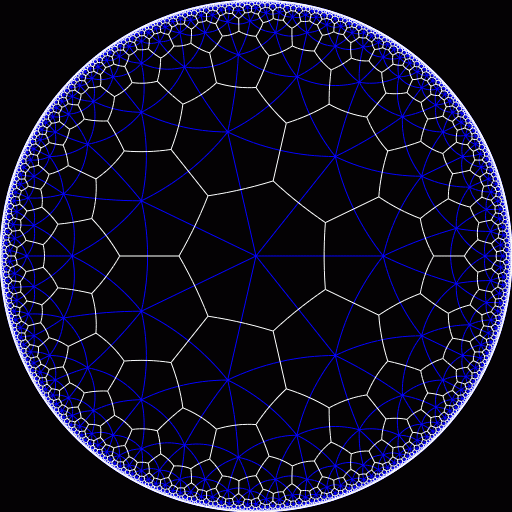
\includegraphics[max width=\linewidth]{../images/7_3.png}}\]

It's called ``\(\{7,3\}\)'', since it's made of 7-sided figures with 3
meeting at each corner.

In this picture there's one heptagon at the center, surrounded by rings
of heptagons that appear smaller (but aren't really --- that's just an
effect of the distortion).

Can we cut out a portion of this tiling and curl it up to get a torus?
No! But, we can curl up a portion to get a 3-holed torus --- like the
surface of a doughnut with three holes. But, we can only do this if we
use precisely 24 heptagons!

Here's how we do it. Here's a picture of 24 heptagons, taken from an old
paper by Klein and Fricke but prettied up a bit:

\begin{enumerate}
\def\labelenumi{\arabic{enumi})}
\setcounter{enumi}{1}
\tightlist
\item
  Tony Smith, Klein's quartic surface,
  \texttt{http://www.valdostamuseum.org/hamsmith/cdomain.html\#tesselations}
\end{enumerate}

\[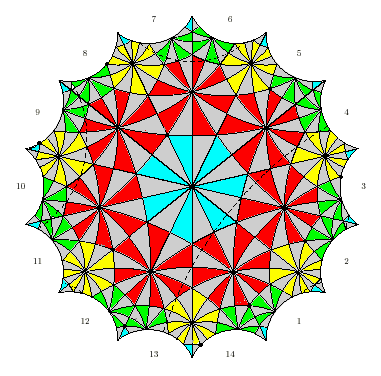
\includegraphics[max width=\linewidth]{../images/Klein168.png}\]

You'll notice they're drawn in a fancy style: each heptagon has been
``barycentrically subdivided'' into 14 right triangles. But don't worry
about that yet; concentrate on the heptagons.

There's a blue heptagon in the middle, 7 red ones touching that, 7
yellow ones touching those, then 7 green ones falling off the edge of
the picture, and 2 blue ones broken into bits all around the corners of
the picture. That's a total of 24 heptagons.

We wrap this thing up into a 3-holed torus using the numbers on the
edges of the picture:

\begin{itemize}
\tightlist
\item
  connect edges 1 and 6
\item
  connect edges 3 and 8
\item
  connect edges 5 and 10
\item
  connect edges 7 and 12
\item
  connect edges 9 and 14
\item
  connect edges 11 and 2
\item
  connect edges 13 and 4
\end{itemize}

In other words, connect edges \(2n+1\) and \(2n+6\) \(\mod 14\). To
connect them the right way, make sure that triangles of the same color
never touch each other.

Here's how to see if you get the idea. Ignore the little triangles; just
pay attention to the heptagons! Then:

Start on any edge of any heptagon and march along in either direction.

Then, when you get to the end, turn left.

Then, when you get to the end, turn right.

Then, when you get to the end, turn left.

Then, when you get to the end, turn right.

Then, when you get to the end, turn left.

Then, when you get to the end, turn right.

Then, when you get to the end, turn left.

Then, when you get to the end, turn right.

You should now be back where you started!!!

These are like the driving directions the devil gives people who ask the
way out of hell. LRLRLRLR and you're right back where you started.

But the resulting Platonic surface is heavenly. It has lots of
symmetries. Each of the 24 heptagons has 7-fold rotational symmetry ---
and amazingly, all these rotations extend to a symmetry of the Platonic
surface!

Now let's talk about those little triangles. Since our surface is made
of 24 heptagons, each chopped into 14 right triangles, there are a total
of \[24 \times 14 = 336\] triangles. And this number is also the number
of symmetries of the Klein quartic, including reflections!

This is no coincidence. We can specify a symmetry by saying where it
sends our favorite right triangle. Since it can go to any other
triangle, there are 336 possibilities. If we exclude reflections, we get
half as many symmetries: \(24 \times 7 = 168\).

By the way, this trick works for ordinary Platonic solids as well. For
example, if we take a dodecahedron and barycentrically subdivide all 12
pentagons, we get \(10 \times 12 = 120\) right triangles. If we pick one
of these as the ``identity element'', we can specify any symmetry by
saying which triangle this triangle gets sent to. So, the set of
triangles becomes a vivid \textbf{picture} of the \(120\)-element
symmetry group of the dodecahedron. It's called the ``Coxeter complex''.
This idea generalizes in many directions, and is incredibly useful.

Anyway\ldots{} there is much more to say about this stuff. For example,
if we take our hyperbolic plane tiled with heptagons and count them
grouped according to how far they are from the central one, we get the
sequence \[7, 7, 14, 21, 35, 56, 91, \ldots\] These are \(7\) times the
Fibonacci numbers!

To dig a bit deeper, though, it helps to think about complex analysis.

If we think of the hyperbolic plane as the unit disc in the complex
plane, this surface becomes a ``Riemann surface'', meaning that it gets
equipped with a complex structure. This was Felix Klein's viewpoint when
he discovered all this stuff in about 1878. He showed this surface could
be described by an incredibly symmetrical quartic equation in 3 complex
variables: \[u^3 v + v^3 w + w^3 u = 0\] where we count two solutions as
the same if they differ by an overall factor. So, it's called ``Klein's
quartic curve''.

(Why a ``curve'' and not a surface? Because it takes one \emph{complex}
number to say where you are on it. We have 3 unknowns and one equation,
but we mod out by an overall factor, so we get something locally
parametrized by one complex number\ldots{} so algebraic geometers call
it a curve.)

You can read Klein's original article translated into English. It's
available online as part of a whole \emph{book} about his incredible
quartic:

\begin{enumerate}
\def\labelenumi{\arabic{enumi})}
\setcounter{enumi}{2}
\tightlist
\item
  Silvio Levy, \emph{The Eightfold Way: the Beauty of Klein's Quartic
  Curve}, MSRI Research Publications \textbf{35}, Cambridge U. Press,
  Cambridge 1999. Also available as
  \texttt{http://www.msri.org/publications/books/Book35/}
\end{enumerate}

This book was put out by the Mathematical Sciences Research Institute in
Berkeley, to celebrate the completion of sculpture of Klein's quartic
curve made by Helaman Ferguson. I must admit that the sculpture leaves
me unmoved. But the curve itself --- ah, that's another story!

For example, Klein's quartic curve turns out to have the maximum number
of symmetries of any 3-holed Riemann surface.

Let's back up a minute and think about a Riemann surface with no holes:
a sphere. There's only one way to make a sphere into a Riemann surface
--- it's called the Riemann sphere. You can think of it as the complex
numbers plus a point at infinity. This has \emph{infinitely} many
symmetries. They're called conformal transformations, and they all look
like this: \[z\mapsto\frac{az+b}{cz+d}\] They form a group called
\(\mathrm{PSL}(2,\mathbb{C})\), since it's the same as the group of
\(2\times2\) complex matrices with determinant \(1\), mod scalars. It's
also the same as the Lorentz group!

There are different ways to make a torus into a Riemann surface, some
with more symmetries than others (see \protect\hyperlink{week124}{``Week
124''}). But, there are always translation symmetries in both
directions, so the symmetry group is always infinite.

On the other hand, a Riemann surface with 2 or more holes can only have
a \emph{finite} group of conformal transformations. In fact, in 1893
Hurwitz proved that a Riemann surface with \(g\) holes has at most
\[84(g - 1)\] For \(g = 3\), this is 168. So, Klein's quartic surface is
as symmetrical as possible! (We don't count reflections here, since they
don't preserve the complex structure --- they're like complex
conjugation.)

Now I should break down and give the best description of Klein's quartic
curve as a Riemann surface. Sitting inside
\(\mathrm{PSL}(2,\mathbb{C})\) is \(\mathrm{PSL}(2,\mathbb{Z})\), where
we only use integers \(a,b,c,d\) in our fractional linear transformation
\[z\mapsto\frac{az+b}{cz+d}\] This subgroup acts on the upper half-plane
\(H\), which is just another way of thinking about the hyperbolic plane.

Sitting inside \(\mathrm{PSL}(2,\mathbb{Z})\) is a group \(\Gamma(7)\)
consisting of guys where the matrix \[
  \left(
    \begin{array}{cc}
      a&b\\c&d
    \end{array}
  \right)
\] is congruent to the identity: \[
  \left(
    \begin{array}{cc}
      1&0\\0&1
    \end{array}
  \right)
\] modulo \(7\). This is an example of a ``congruence subgroup''; these
serve to relate complex analysis to number theory in lots of cool ways.
In particular, Klein's quartic curve is just \[H/\Gamma(7)\] Since
\(\Gamma(7)\) is a normal subgroup of \(\mathrm{PSL}(2,\mathbb{Z})\),
the quotient group
\[\mathrm{PSL}(2,\mathbb{Z})/\Gamma(7) = \mathrm{PSL}(2,\mathbb{Z}/7)\]
acts as symmetries of Klein's quartic curve. And, this group has 168
elements!

In fact, this group is the second smallest nonabelian simple group. The
smallest one is the rotational symmetry group of the icosahedron, which
has 60 elements. This group is actually
\(\mathrm{PSL}(2,\mathbb{Z}/5)\), and Klein had run into it in his work
on the icosahedron and quintic equations (see
\protect\hyperlink{week213}{``Week 213''}). So, it's actually far from
sheer luck that he then moved on to \(\mathrm{PSL}(2,\mathbb{Z}/7)\) and
ran into his wonderful quartic curve.

By the way, this \(168\)-element group is also known as
\(\mathrm{PSL}(3,\mathbb{Z}/2)\) --- the symmetry group of the ``Fano
plane''. This is a name for the projective plane over \(\mathbb{Z}/2\).
The Fano plane is closely related to the octonions:

\begin{enumerate}
\def\labelenumi{\arabic{enumi})}
\setcounter{enumi}{2}
\tightlist
\item
  John Baez, ``The Fano plane'',
  \texttt{http://math.ucr.edu/home/baez/octonions/node4.html}
\end{enumerate}

\[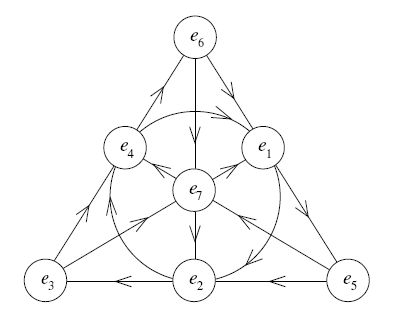
\includegraphics[max width=\linewidth]{../images/fano.jpg}\]

So in fact, our \(168\)-element group acts on the set of octonion
multiplication tables:

\begin{enumerate}
\def\labelenumi{\arabic{enumi})}
\setcounter{enumi}{3}
\item
  Tony Smith, ``Octonion products'',
  \texttt{http://www.valdostamuseum.org/hamsmith/480op.html}
\item
  Geoffrey Dixon, ``Octonion multiplication tables'',
  \texttt{http://www.7stones.com/Homepage/octotut0.html}
\end{enumerate}

And, as James Dolan just noted today, and Tony Smith seems to have known
all along, there's a way to draw the Fano plane that even \emph{looks}
like the diagram Klein and Fricke used to build the Klein quartic.
Here's a picture drawn by Burkard Polster, author of ``The Mathematics
of Juggling'' and ``Geometries on Surfaces'':

\[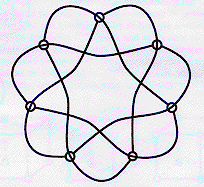
\includegraphics[max width=\linewidth]{../images/symfano.png}\]

So, something interesting is going on, and I want to know what it is!

By the way, fans of the quaternions and octonions may like this review
of Conway and Smith's book:

\begin{enumerate}
\def\labelenumi{\arabic{enumi})}
\setcounter{enumi}{5}
\tightlist
\item
  John Baez, ``review of \emph{On Quaternions and Octonions: Their
  Geometry, Arithmetic and Symmetry}, by John H. Conway and Derek A.
  Smith'', \emph{Bull. Amer. Math. Soc.} \textbf{42} (2005), 229--243.
  Available at \texttt{http://www.ams.org/bull/2005-42-02/} and
  \texttt{http://math.ucr.edu/home/baez/octonions/node24.html}
\end{enumerate}

It's packed with cool pictures and weird facts --- a more refined
version of the material in \protect\hyperlink{week193}{``Week 193''} and
\protect\hyperlink{week194}{``Week 194''}.

It builds up to a kind of crazy climax in which I describe how when you
pack spheres as densely as possible in 8 dimensions, each sphere touches
240 others\ldots{} and if you look at the 240 neighbors of a given
sphere, each one of those neighbors touches 56 other neighbors. Then I
explain how this gives rise to a \(56\)-dimensional representation of
the exceptional group \(\mathrm{E}_7\) --- its smallest nontrivial
representation! And, how it gives rise to a \(57\)-dimensional manifold
on which the exceptional group \(\mathrm{E}_8\) acts --- the smallest
space on which it acts nontrivially!

Bertram Kostant is one of the real gurus of Lie theory. He teaches at
MIT, and he has a strong fondness for exceptional Lie groups. When he
saw this review of mine, he mentioned a couple of other papers that
construct the \textbf{57}-dimensional space on which \(\mathrm{E}_8\)
acts:

\begin{enumerate}
\def\labelenumi{\arabic{enumi})}
\setcounter{enumi}{6}
\item
  Ranee Brylinski and Bertram Kostant, ``Lagrangian models of minimal
  representations of \(\mathrm{E}_6\), \(\mathrm{E}_7\), and
  \(\mathrm{E}_8\)'', in \emph{Functional Analysis on the Eve of the
  21st Century}, vol.~\textbf{1}, Progress in Math. \textbf{131},
  Birkhauser, Boston, 1995, pp.~13--53.

  Bertram Kostant, ``Minimal coadjoint orbits and symplectic
  induction'', in \emph{The Breadth of Symplectic and Poisson geometry},
  391--422, Progress in Math. \textbf{232}, Birkhauser, Boston, 2005.
  Also available as \texttt{http://www.arXiv.org/abs/math.SG/0312252}
\end{enumerate}

I've got to read these sometime.

Having the number 56 on my brain, I can't resist nothing that if you
take Klein's quartic curve tiled by heptagons, and you count the
vertices, you get \[24 \times 7 / 3 = 56\] since each vertex is shared
by 3 heptagons. I'm hoping this is not a coincidence!

Okay, that's all for this week, except for some silly stuff\ldots.

First of all, speaking of octonions, Geoff Corbishley just told me that
their inventor, John Thomas Graves, is a relative of Robert Graves ---
the author of ``I Claudius''.

Second of all, I hope you've figured out the puzzle I gave at the
beginning of this Week. The phrase is ``24-7'', as in ``we're working on
it 24-7''. 24 hours a day, 7 days a week, makes 168 hours per week!

Finally, speaking of numerology, this number 168 is related to why the
days of the week have the names they do! I explained why in
\protect\hyperlink{week175}{``Week 175''}, but I'll remind you:

Astrologers liked to list the planets in order of decreasing orbital
period, counting the sun as having a period of one year, and the moon as
period of one month:

\begin{longtable}[]{@{}ll@{}}
\toprule
Planet & Orbital period\tabularnewline
\midrule
\endhead
Saturn & 29 years\tabularnewline
Jupiter & 12 years\tabularnewline
Mars & 687 days\tabularnewline
Sun & 365 days\tabularnewline
Venus & 224 days\tabularnewline
Mercury & 88 days\tabularnewline
Moon & 29.5 days\tabularnewline
\bottomrule
\end{longtable}

For the purposes of astrology they wanted to assign a planet to each
hour of each day of the week. To do this, they assigned Saturn to the
first hour of the first day, Jupiter to the second hour of the first
day, and so on, cycling through the list of planets over and over, until
each of the \(24 \times 7 = 168\) hours was assigned a planet. Each day
was then named after the first hour in that day. Since 24 mod 7 equals
3, this amounts to taking the above list and cycling around it, reading
off every third planet:

\begin{longtable}[]{@{}ll@{}}
\toprule
\endhead
Saturn & Saturday\tabularnewline
Sun & Sunday\tabularnewline
Moon & Monday\tabularnewline
Mars & Tuesday\tabularnewline
Mercury & Wednesday\tabularnewline
Jupiter & Thursday\tabularnewline
Venus & Friday\tabularnewline
\bottomrule
\end{longtable}

And that's how they got listed in this order! At least, this is what the
Roman historian Dion Cassius (AD 150--235) claims. Nobody knows for
sure.

\begin{center}\rule{0.5\linewidth}{0.5pt}\end{center}

\textbf{Addendum:} Mike Stay took Don Hatch's picture and drew numbers
from 1 to 24 showing how to identify heptagons in order to get the Klein
quartic curve:
\[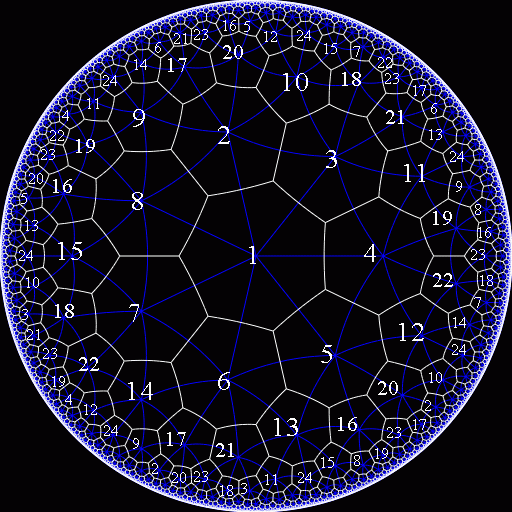
\includegraphics[max width=\linewidth]{../images/7-3.png}\]

Gerard Westendorp had some interesting comments on what I wrote:

\begin{quote}
If you take Euler's formula \[V+F-E = 2-2\times\text{holes}\] then you
can figure out that for a \((7,3)\) tiling with \(N\) heptagons, you
have \[
  \begin{aligned}
    V &= \frac{7N}{3}
  \\F &= N
  \\E &= \frac{7N}{2}    
  \end{aligned}
\] so that \[N = 12\times(\text{holes}-1)\] Here's the table of
solutions:

\begin{longtable}[]{@{}ll@{}}
\toprule
holes & \(N\)\tabularnewline
\midrule
\endhead
0 & -12\tabularnewline
1 & 0\tabularnewline
2 & 12\tabularnewline
3 & 24\tabularnewline
4 & 36\tabularnewline
\(\vdots\) & \(\vdots\)\tabularnewline
\bottomrule
\end{longtable}

So indeed, there are no solutions for 0 holes (sphere) or 1 hole
(torus). But a \(2\)-holed torus should be possible, as well as the
\(24\)-faced \(3\)-holed one.

Anyway, see if I can visualise the \(3\)-holed one.

If you start with a sphere, i.e.~genus 0, and drill a tunnel through it,
you will get a genus 1 object. On the outer surface, you see 2 holes,
one for each side of the ``tunnel''. (I use the word ``tunnel'' for
something into a 3D object, and ``hole'' for something in a 2D surface.)

Next, you can drill a second tunnel, and get a genus 2 object, and you
would see 4 holes on the outer surface. But a nice trick is to drill not
to the outer surface, but to a secret ``cave'' in the middle where you
meet the first tunnel. Here you stop drilling. To complete the genus-3
object, you drill the third tunnel again not to the outer surface, but
to the central cave. Thus, you get and object with genus 3, which has 4
holes on its outer surface, each leading to a central cave.

Confusingly, 4 tunnels to a central cave is topologically the same as 3
separate tunnels! The trick is that tunnels do not have to end on the
outer surface, the inner surface is topologically the same.

OK, so we have an object with 4 holes on its outer surface. 4 holes
\(\to\) tetrahedron\ldots{}

I built a cardboard model of a tetrahedron with a central cave.
Truncated tetrahedrons together with tetrahedrons can fill space. So you
can stack 4 truncated tetrahedra on top of each other, leaving a hole in
the shape of an imaginary 5th one. Then use tetrahedra to fill up some
gaps. This was basically the shape I built out of cardboard. Then, I
spent rather a long time trying to tile this with heptagons. A clue to a
solution was that a triangulation of the surface I made had 120
triangle, and \(120 = 24\times5\). What is so good about 5? Well, 5
triangles stuck together have 7 outer sides, sop they are a kind of
pseudo heptagons. Anyway, I got a bit frustrated, and did not find a
nice tiling.

As I was trying to figure it out, I found this site:

\begin{quote}
\texttt{http://www.math.uni-siegen.de/wills/klein/}
\end{quote}

It has some nice pictures.

\begin{quote}
These are like the driving directions the devil gives people who ask the
way out of hell. LRLRLRLR and you're right back where you started.
\end{quote}

Btw, this works the same on other polyhedra, e.g.~the cube.

\begin{quote}
Saturn (Saturday) Sun (Sunday) Moon (Monday) Mars (Tuesday) Mercury
(Wednesday) Jupiter (Thursday) Venus (Friday)
\end{quote}

My French is not so good, but in French some names look more convincing:

\begin{itemize}
\tightlist
\item
  tuesday = mardi (Mars?)
\item
  wednesday = mercredi (Mercury?)
\item
  thursday = jeudi (Jove?)
\item
  friday = vendredi (Venus?)
\end{itemize}

Gerard
\end{quote}

I replied:

\begin{quote}
Gerard Westendorp wrote:

\begin{quote}
John Baez wrote:
\end{quote}

\begin{quote}
\begin{quote}
It's called ``\(\{7,3\}\)'', since it's made of 7-sided figures with 3
meeting at each corner.
\end{quote}
\end{quote}

\begin{quote}
\begin{quote}
Can we cut out a portion of this tiling and curl it up to get a torus?
No! But, we can curl up a portion to get a \(3\)-holed torus --- like
the surface of a doughnut with three holes. But, we can only do this if
we use precisely 24 heptagons!
\end{quote}
\end{quote}

\begin{quote}
If you take Euler's formula {[}\ldots.{]}
\end{quote}

\begin{quote}
So indeed, there are no solutions for 0 holes (sphere), 1 hole( torus).
But a \(2\)-holed torus should be possible, as well as the \(24\)-faced
\(3\)-holed one.
\end{quote}

I was going to talk about this, but I figured my article was getting too
long.

Indeed, Euler's formula also allows the possibility of a
\emph{\(2\)-holed} torus tiled with 12 heptagons meeting 3 at each
corner.

But this does not prove such a tiling is possible. I don't know if it
is! Someone should try it.

However: even if such a tiling exists, it's not possible for each
rotational symmetry of each heptagon to extend to a symmetry of the
whole tiled surface. What's marvelous about the 3-holed case is that
they all do --- at least if you do things correctly. This is what makes
the Klein quartic a full-fledged ``Platonic surface''.

If you look here:

\begin{itemize}
\tightlist
\item
  Hermann Karcher and Mattias Weber, ``The Geometry of Klein's Riemann
  Surface'', in \emph{The Eightfold Way: the Beauty of Klein's Quartic
  Curve}, ed.~Silvio Levy, MSRI Research Publications \textbf{35},
  Cambridge U. Press, Cambridge 1999. Also available as
  \href{http://www.msri.org/publications/books/Book35/files/karcher.pdf}{PDF}
  and
  \href{http://www.msri.org/publications/books/Book35/files/karcher.ps.gz}{gzipped
  Postscript}.
\end{itemize}

you'll see that Karcher and Weber study Platonic surfaces using Euler's
formula.

On pages 13--19 they consider Platonic surfaces with 2 holes. On page 19
they give a clever proof that no tiling of the \(2\)-holed torus by
heptagons meeting 3 at each corner can be a Platonic surface. The proof
is so clever that I don't understand it.

(Warning: their article starts on page 9.)

\begin{quote}
Anyway, see if I can visualise the 3-holed one.
\end{quote}

I wish I could visualize it myself.

\begin{quote}
As I was trying to figure it out, I found this site:

\begin{quote}
\texttt{http://www.math.uni-siegen.de/wills/klein/}
\end{quote}

It has some nice pictures.
\end{quote}

These pictures are interesting, but what I'd really like is a nice
picture of a \(3\)-holed torus, not weird or crumpled up, which is tiled
by 24 heptagons just like the Klein quartic.

The heptagons can't all be regular if the torus is embedded in
\(\mathbb{R}^3\), since there's no way to embed a compact surface of
constant negative curvature in \(\mathbb{R}^3\). But, you \emph{can} get
the \emph{topology} correct and still have the torus embedded in
\(\mathbb{R}^3\).

If anyone draws such a picture, and I think it looks nice, I'd love to
put it on This Week's Finds!

If anyone wants instructions on how such a surface should be made, look
above, where Mike Stay has kindly drawn numbers from 1--24 on a portion
of the hyperbolic plane tiled with heptagons. These numbers indicate how
to identify heptagons to get the Klein quartic. For example, all the
heptagons labelled ``21'' are really the same heptagon in the Klein
quartic.

\begin{quote}
\begin{quote}
Saturn (Saturday) Sun (Sunday) Moon (Monday) Mars (Tuesday) Mercury
(Wednesday) Jupiter (Thursday) Venus (Friday)
\end{quote}
\end{quote}

\begin{quote}
My French is not so good, but in French some names look more convincing:

\begin{itemize}
\tightlist
\item
  tuesday = mardi (Mars?)
\item
  wednesday = mercredi (Mercury?)
\item
  thursday = jeudi (Jove?)
\item
  friday = vendredi (Venus?)
\end{itemize}
\end{quote}

Yes, this because most of the English names for planets come from Latin,
and French is more like Latin.

English is more complicated, but I'm so used to it that I forgot people
might find the connection to Latin mysterious:

\begin{itemize}
\tightlist
\item
  ``Tuesday'' comes from ``Tiu'' or ``Tyr'', an ancient Germanic god of
  war whom the Romans identified with Mars. We see traces of this in the
  German ``Dienstag'' as well.
\item
  ``Wednesday'' comes from ``Woden'' or ``Odin'', a Germanic god whom
  the Romans identified with Mercury. Modern German uses ``Mittwoch''
  instead, which means ``mid-week''.
\item
  ``Thursday'' comes from ``Thor'', a Germanic thunder god whom the
  Romans identified with Jupiter. Modern German uses ``Donnerstag''
  instead, with ``Donner'' meaning ``thunder''.
\item
  ``Friday'' comes from ``Freya'' or ``Frigga'', a Germanic goddess of
  married love whom the Romans identified with Venus. The German
  ``Freitag'' is very similar.
\end{itemize}
\end{quote}

\begin{center}\rule{0.5\linewidth}{0.5pt}\end{center}



\hypertarget{week215}{%
\section{May 9}\label{week215}}

This week I'd like to report on some cool things people have been
explaining to me. The science fiction writer Greg Egan has been helping
me understand Klein's quartic curve, and the mathematician Darin Brown
has been explaining the analogy between geodesics and prime numbers. The
two subjects even overlap slightly!

Last week I talked about Klein's quartic curve. This led Gerard
Westendorp and Mike Stay to draw some pictures of it, and their ideas
helped Greg Egan create this really nice picture:

\begin{enumerate}
\def\labelenumi{\arabic{enumi})}
\tightlist
\item
  Greg Egan, ``Klein's quartic curve'',
  \texttt{http://math.ucr.edu/home/baez/mathematical/KleinDual.png}
\end{enumerate}

\[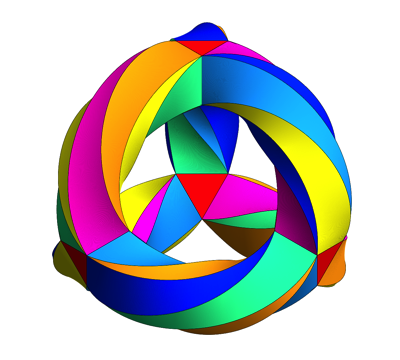
\includegraphics[max width=\linewidth]{../images/KleinDual.png}\] It
looks sort of tetrahedral at first glance, but if you look carefully
you'll see that topologically speaking, it's a \(3\)-holed torus. It's
tiled by triangles, with 7 meeting at each vertex. So, it's the Klein
quartic curve!

Perhaps I should explain. Last week I talked about a tiling of the
hyperbolic plane by regular heptagons with 3 heptagons meeting at each
vertex. Dual to this is a tiling of the hyperbolic plane by equilateral
triangles with 7 triangles meeting at each vertex. We can take a
quotient space of this by a certain symmetry group and get a \(3\)-holed
torus tiled by 56 triangles with 7 meeting at each vertex. This is what
Egan drew!

With this picture you can almost \emph{see} the 168 symmetries of
Klein's quartic curve.

First, you can take any vertex and twist it, causing the 7 triangles
that meet at this vertex to cycle around. It's not obvious that this is
a symmetry of the whole tiled surface, but it is. This gives a
\(7\)-element symmetry group.

Second, the whole thing looks like a tetrahedron, so it inherits the
rotational symmetries of a tetrahedron. This gives a more obvious
\(12\)-element symmetry group.

\(7 \times 12 = 84\), so how do we get a total of 168 symmetries?

Well, there's also a \(2\)-fold symmetry that corresponds to turning the
tetrahedron inside out! And Egan made a wonderful \emph{movie} of this.
If a picture is worth a thousand words, this is worth about a million:

\begin{enumerate}
\def\labelenumi{\arabic{enumi})}
\setcounter{enumi}{1}
\tightlist
\item
  Greg Egan, ``Turning Klein's quartic curve inside out'',
  \texttt{http://math.ucr.edu/home/baez/mathematical/KleinDualInsideOut.gif}
\end{enumerate}

So, we get a total of \(7 \times 24 = 168\) symmetries.

Even better, if you watch carefully, you'll see that the tetrahedron in
Egan's movie gets \emph{reflected} as it turns inside out. More
precisely, if you follow the four corners of the tetrahedron, you'll see
that two come back to where they were, while the other two get switched.
So, this symmetry acts as a reflection, or odd permutation, of the 4
corners. The rotations act as even permutations of the corners.

This means that the Klein quartic has 24 symmetries forming a group
isomorphic to the rotation/reflection symmetry group of a tetrahedron.
Algebraically speaking, this group is \(S_4\): the permutations of 4
things.

This group is also the rotational symmetry group of a cube. In fact,
Egan was able to spot a hidden cube lurking in his picture! Can you?
\[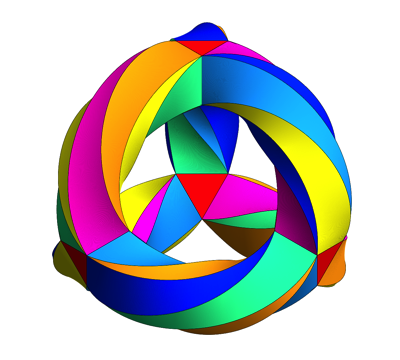
\includegraphics[max width=\linewidth]{../images/KleinDual.png}\] If
you look carefully, you'll see each corner of his tetrahedral gadget is
made of a little triangular prism with one triangle facing out and one
facing in: for example, the pink triangle staring you right in the face,
or the light blue one on top. Since \(4 \times 2 = 8\), there are 8 of
these triangles. Abstractly, we can think of these as the 8 corners of a
cube! They aren't really, but we can pretend. The way these 8 triangles
come in pairs corresponds to how the vertices of a cube come in
diagonally opposite pairs.

Using this, you can see that the group \(S_4\) acts on these 8 triangles
in precisely the same way it acts via rotations on the vertices of a
cube.

In fact, you can even draw a \emph{picture} of a cube on the Klein
quartic by drawing suitable curves that connect the centers of these 8
triangles! It's horribly distorted, but topologically correct. Part of
the distortion is caused by embedding the Klein quartic in ordinary 3d
Euclidean space. If we gave the Klein quartic the metric it inherits
from the hyperbolic plane, the edges of the cube would be geodesics.

This remark also helps us see something else. The Klein quartic is tiled
by 56 triangles. 8 of them give the cube we've just been discussing. In
Egan's picture these triangles look special, since they lie at the
corners of his tetrahedral gadget. But this is just an illusion caused
by embedding the Klein quartic in 3d space. In reality, the Klein
quartic is perfectly symmetrical: every triangle is just like every
other. So in fact there are lots of these cubes, and every triangle lies
in some cube.

But this is where it gets really cool. In fact, each triangle lies in
just \emph{one} cube. So, there's precisely one way to take the 56
triangles and divide them into 7 bunches of 8 so that each bunch forms a
cube.

So: the symmetry group of the Klein quartic acts on the set of cubes,
which has 7 elements.

But as I explained last week, this symmetry group also acts on the Fano
plane, which has 7 points.

This suggests that cubes in the Klein quartic naturally correspond to
points of the Fano plane. And Egan showed this is true!

He showed this by showing more. The Fano plane also has 7 lines. What 7
things in the Klein quartic do these lines correspond to?

\emph{Anticubes!}

You see, the cubes in the Klein quartic have an inherent handedness to
them. You can go between the 8 triangles of a given cube by following
certain driving directions, but these driving directions involve some
left and right turns. If you follow the mirror-image driving directions
with ``left'' and ``right'' switched, you'll get an \emph{anticube}.

Apart from having the opposite handedness, anticubes are just like
cubes. In particular, there's precisely one way to take the 56 triangles
and divide them into 7 bunches of 8 so that each bunch forms an
anticube.

Here's a picture:

\begin{enumerate}
\def\labelenumi{\arabic{enumi})}
\setcounter{enumi}{2}
\tightlist
\item
  Greg Egan, Cubes and anticubes in the Klein quartic curve,
  \texttt{http://math.ucr.edu/home/baez/KleinFigures.gif}
\end{enumerate}

\[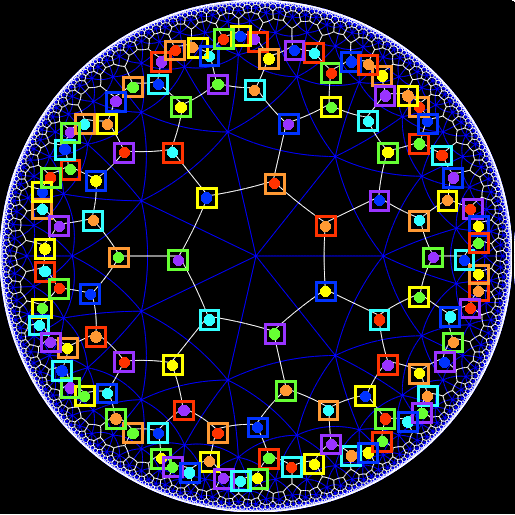
\includegraphics[max width=\linewidth]{../images/KleinFigures.png}\]
Each triangle has a colored circle and a colored square on it. There are
7 colors. The colored circle says which of the 7 \emph{cubes} the
triangle belongs to. The colored square says which of the 7
\emph{anticubes} it belongs to.

If you stare at this picture for a few hours, you'll see that each cube
is completely disjoint from precisely 3 anticubes. Similarly, each
anticube is completely disjoint from precisely 3 cubes.

This is just like the Fano plane, where each point lies on 3 lines, and
each line contains 3 points!

So, we get a vivid way of seeing how every figure in the Fano plane
corresponds to some figure in the Klein quartic curve. This is why they
have the same symmetry group.

This is an excellent example of Klein's Erlangen program for reducing
geometry to group theory, which I discussed in
\protect\hyperlink{week213}{``Week 213''}. Here we are beginning to see
how two superficially different geometries are secretly the same:

\begin{longtable}[]{@{}ll@{}}
\toprule
Fano plane & Klein's quartic curve\tabularnewline
\midrule
\endhead
7 points & 7 cubes\tabularnewline
7 lines & 7 anticubes\tabularnewline
incidence of points and lines & disjointness of cubes and
anticubes\tabularnewline
\bottomrule
\end{longtable}

However, we're only half done! We've seen how to translate simple
figures and indicence relations in the Fano plane to complicated ones in
Klein's quartic curve. But, we haven't figured out translate back!

\begin{longtable}[]{@{}ll@{}}
\toprule
Klein's quartic curve & Fano plane\tabularnewline
\midrule
\endhead
24 vertices & ???\tabularnewline
84 edges & ???\tabularnewline
56 triangular faces & ???\tabularnewline
incidence of vertices and edges & ???\tabularnewline
incidence of edges and faces & ???\tabularnewline
\bottomrule
\end{longtable}

Here I'm talking about the tiling of Klein's quartic curve by 56
equilateral triangles. We could equally well talk about its tiling by 24
regular heptagons, which is the Poincare dual. Either way, the puzzle is
to fill in the question marks. I don't know the answer!

To conclude --- at least for now --- I want to give the driving
directions that define a ``cube'' or an ``anticube'' in Klein's quartic
curve. Say you're on some triangle and you want to get to a nearby
triangle that belongs to the same cube. Here's what you do:

\begin{quote}
hop across any edge,\\
turn right,\\
hop across the edge in front of you,\\
turn left,\\
then hop across the edge in front of you.
\end{quote}

Or, suppose you're on some triangle and you want to get to another
that's in the same anticube. Here's what you do:

\begin{quote}
hop across any edge,\\
turn left,\\
hop across the edge in front of you,\\
turn right,\\
then hop across the edge in front of you.
\end{quote}

(If you don't understand this stuff, look at the picture above and see
how to get from any circle or square to any other circle or square of
the same color.)

You'll notice that these instructions are mirror-image versions of each
other. They're also both \(1/4\) of the ``driving directions from hell''
that I described last time. In other words, if you go LRLRLRLR or
RLRLRLRL, you wind up at the same triangle you started from. You'll have
circled around one face of a cube or anticube!

In fact, your path will be a closed geodesic on the Klein quartic
curve\ldots{} like the long dashed line in Klein and Fricke's original
picture:

\begin{enumerate}
\def\labelenumi{\arabic{enumi})}
\setcounter{enumi}{3}
\tightlist
\item
  Klein and Fricke, Klein's quartic curve with geodesic,
  \texttt{http://math.ucr.edu/home/baez/Klein168.gif}
\end{enumerate}

\[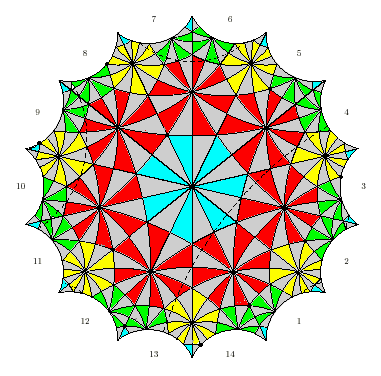
\includegraphics[max width=\linewidth]{../images/Klein168.png}\]

Next, a little about geodesics and prime numbers. I've just been talking
a little about geodesics in the Klein quartic, which is the quotient

\[H/G\]

of the hyperbolic plane \(H\) by a certain group \(G\) which I explained
last week. This group, usually called \(\Gamma(7)\), is a nice example
of a ``Fuchsian group'' --- that is, a discrete subgroup of the
isometries of the hyperbolic plane.

Darin Brown and his thesis advisor Jeff Stopple at U. C. Santa Barbara
have been thinking about geodesics in \(H/G\) for other Fuchsian groups
\(G\), and their relation to number theory:

\begin{enumerate}
\def\labelenumi{\arabic{enumi})}
\setcounter{enumi}{4}
\item
  Jeff Stopple, ``A reciprocity law for prime geodesics'', \emph{J.
  Number Theory} \textbf{29} (1988), 224--230.
\item
  Darin Brown, \emph{Lifting properties of prime geodesics on hyperbolic
  surfaces}, Ph.D.~thesis, U. C. Santa Barbara, 2004.
\end{enumerate}

I'd really like to learn about this, because it connects all sorts of
stuff I dream of understanding someday, especially quantum chaos
(\protect\hyperlink{week190}{``Week 190''}), zeta functions in physics
and number theory (\protect\hyperlink{week199}{``Week 199''}), and
Galois theory as a theory of covering spaces
(\protect\hyperlink{week205}{``Week 205''}). Also, it involves a big
mysterious analogy, and I always like those!

I don't understand this stuff well enough to try a full-fledged
explanation yet, so I'll just give a vague sketch. A ``prime geodesic''
in a Riemannian manifold \(X\) is a closed geodesic
\[f\colon S^1 \to X\] that cycles around just once. In other words,
\(f\) should be one-to-one.

We say a closed geodesic is the ``\(n\)th power'' of a prime one if it's
just like the prime one but it cycles around \(n\) times. Every closed
geodesic is the \(n\)th power of a prime one in a unique way.

If we have a Fuchsian group \(G\), \(H/G\) is a surface with a
Riemannian metric. It looks locally like the hyperbolic plane, so it's
called a ``hyperbolic surface''. And, we can look at prime geodesics in
it.

If \(G'\) is a subgroup of \(G\), we get a covering map \[H/G' \to H/G\]
so we can ask about lifting prime geodesics in \(H/G\) to closed
geodesics in \(H/G'\). There can be a bunch of ways to do this, so we
say a prime geodesic in \(H/G\) ``splits'' into powers of prime
geodesics up in \(H/G'\).

If you know any number theory --- reading
\protect\hyperlink{week205}{``Week 205''} should be enough --- this
should remind you of how a prime ideal in some algebraic number field
can ``split'' into prime ideals in an extension of this field, and/or
``ramify'' into powers of prime ideals.

And indeed, Darin Brown has found a big mysterious analogy that goes
like this:

\begin{longtable}[]{@{}ll@{}}
\toprule
\endhead
Number field \(K\) & Hyperbolic surface \(H/G\)\tabularnewline
Field extension \(K'\) of \(K\) & Covering
\(p\colon H/G' \to H/G\)\tabularnewline
Galois group \(\mathrm{Gal}(K'/K)\) & Deck transformation group
\(\mathrm{Aut}(p)\)\tabularnewline
Prime ideal \(Q\) of \(K\) & Prime geodesic \(f\) in
\(H/G\)\tabularnewline
Prime ideal \(Q'\) lying over \(Q\) & Prime geodesic \(f'\) lying over
\(f\)\tabularnewline
Splitting of prime ideal \(Q\) of \(K'\) & Lifting of prime geodesic
\(f\) to \(H/G'\)\tabularnewline
Norm \(N(Q)\) of ideal \(Q\) & Norm \(N(f)\) of closed geodesic
\(f\)\tabularnewline
Frobenius conjugacy class of \(Q\) & Frobenius conjugacy class of
\(f\)\tabularnewline
Artin \(L\)-function & Selberg zeta function\tabularnewline
\bottomrule
\end{longtable}

(Here by ``prime ideal of \(K\)'' we mean a prime ideal in the ring of
algebraic integers of \(K\).)

But this is more than an analogy: there's even a way to associate number
fields to certain hyperbolic surfaces! The reason is that often Fuchsian
groups will consist of matrices whose entries lie in some number field.

I would like to understand the Selberg zeta function and its relation to
quantum mechanics. The Selberg zeta function is related to closed
geodesics, which are periodic classical trajectories, while the zeta
function of a Laplacian is related to periodic \emph{quantum}
trajectories (namely eigenfunctions of the Laplacian). So, the two are
related. I know there's a lot of cool stuff going on here --- especially
since the motion of a particle on a hyperbolic surface tends to be
chaotic, so ``quantum chaos'' rears its ugly head. But, I don't
understand any of the details.

In some notes on quantum chaos, Gutzwiller wrote:

\begin{quote}
The classical periodic orbits are a crucial stepping stone in the
understanding of quantum mechanics, in particular when then classical
system is chaotic. This situation is very satisfying when one thinks of
Poincaré who emphasized the importance of periodic orbits in classical
mechanics, but could not have had any idea of what they could mean for
quantum mechanics. The set of energy levels and the set of periodic
orbits are complementary to each other since they are essentially
related through a Fourier transform. Such a relation had been found
earlier by the mathematicians in the study of the Laplacian operator on
Riemannian surfaces with constant negative curvature. This led to
Selberg's trace formula in 1956 which has exactly the same form, but
happens to be exact. The mathematical proof, however, is based on the
high degree of symmetry of these surfaces which can be compared to the
sphere, although the negative curvature allows for many more different
shapes.
\end{quote}

When I get serious, I'll read these:

\begin{enumerate}
\def\labelenumi{\arabic{enumi})}
\setcounter{enumi}{6}
\item
  M. C. Gutzwiller, \emph{Chaos in Classical and Quantum Mechanics},
  Springer, Berlin, 1990.
\item
  Predrag Cvitanovic, Roberto Artuso, Per Dahlqvist, Ronnie Mainieri,
  Gregor Tanner, Gabor Vattay, Niall Whelan and Andreas Wirzba,
  \emph{Chaos: Classical and Quantum}, available at
  \texttt{http://www.nbi.dk/ChaosBook/}
\item
  Svetlana Katok, \emph{Fuchsian Groups}, U. Chicago Press, Chicago,
  1992.
\item
  J. Elstrodt, F. Grunewald, and J. Mennicke, \emph{Groups Acting on
  Hyperbolic Space}, Springer, Berlin, 1998.
\item
  Peter Sarnak, ``Quantum chaos, symmetry and zeta functions'', in
  \emph{Current Developments in Mathematics}, 1997, eds R. Bott et al.,
  International Press, Boston, 1999, pp.~127--159.
\item
  C. Schmit, ``Quantum and classical properties of some billiards on the
  hyperbolic plane'', in \emph{Chaos and Quantum Physics}, eds.~M.-J.
  Giannoni et al., Elsevier, New York, 1991, pp.~333--369.
\end{enumerate}

For a nice pop treatment of quantum chaos and the Riemann hypothesis,
try this:

\begin{enumerate}
\def\labelenumi{\arabic{enumi})}
\setcounter{enumi}{12}
\tightlist
\item
  Martin Gutzwiller, ``Quantum chaos'', \emph{Scientific American},
  January 1992. Also available at
  \texttt{http://www.maths.ex.ac.uk/\textasciitilde{}mwatkins/zeta/quantumchaos.html}
\end{enumerate}

\begin{center}\rule{0.5\linewidth}{0.5pt}\end{center}

\textbf{Addendum:} Here is some email I got from Greg Egan and Toby
Bartels, and a post from Darin Brown which corrects some mistakes and
answers some questions raised by my pal Squark.

Greg Egan wrote me the following after I suggested a relation between
the Klein quartic curve and 3d Minkowski spacetime over the field
\(\mathbb{Z}/7\) --- a relation that he later exploited in some
fascinating ways.

\begin{quote}
\begin{verbatim}
Hi

Thanks for all the Lorentz group stuff!  This will take me a while to 
digest.

In the meantime, here are some more translations between the geometries.

Every cube intersects 4 anticubes, and any pair of cubes, between them, 
intersect 6 anticubes (two of the 4 for each will always be shared).  So 
together the pair of cubes single out one anticube:  the 7th one that 
neither of them intersect.  This is analogous to the fact that any two 
Fano points single out a Fano line.

I'll write anti({c1,c2}) for the anticube singled out by a pair of cubes, 
and similarly cube({a1,a2}) for the cube singled out by a pair of 
anticubes.  In the scheme used in this diagram:
\end{verbatim}

\[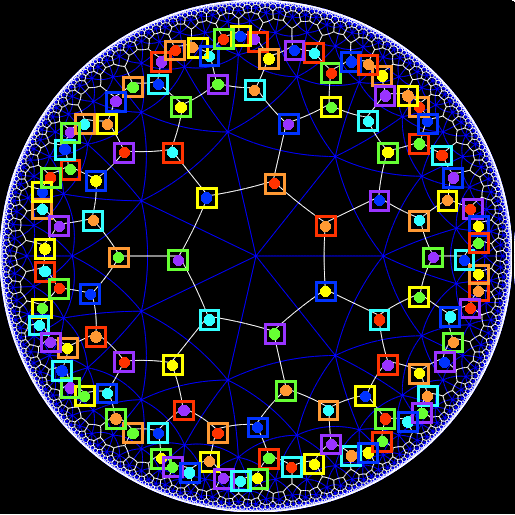
\includegraphics[max width=\linewidth]{../images/KleinFigures.png}\]
both functions have identical outputs for the same input colours:

\begin{verbatim}
    anti({c1,c2})  and  cube({a1,a2})
    =================================

    R   O   Y   G   LB  P   DB
   ----------------------------
R  | -   DB  R   DB  Y   Y   R
O  | DB  -   P   DB  P   O   O
Y  | R   P   -   LB  P   LB  R
G  | DB  DB  LB  -   G   LB  G
LB | Y   P   P   G   -   Y   G
P  | Y   O   LB  LB  Y   -   O
DB | R   O   R   G   G   O   -
   ----------------------------

Now for some actual translations.

Klein's Quartic Curve      Fano plane
---------------------      ----------

28 pairs of opposite       28 choices of a point
triangular faces           and a non-incident line,
                           {p,l}.

                              p1
                              (*)

                           ----------- l1

                           7 x 4 = 28

In Klein's quartic curve, we specify a pair of opposite triangular faces 
by picking one of seven cubes, then one of four anticubes that intersect 
it.  The intersection is a pair of triangular faces which are diagonally 
opposite each other both on the cube and on the anticube.  The 56 order-3 
elements of G preserve these pairs of triangular faces, and consist of 
rotations by 1/3 and 2/3 turns for each such pair.

Triangular faces           Pairings of points and
sharing an edge            non-incident lines {p1,l1} and
                           {p2,l2} having p1 incident on l2 and
                           p2 incident on l1.

                               p1
                           ----(*)----- l2

                           ----(*)----- l1
                               p2

In Klein's quartic curve, whenever two triangular faces share an edge, 
the cube each face belongs to will be disjoint from the anticube that 
the other face belongs to.  This can be checked by noting that the colour 
of the anticube appears in the row for anti(c,.).

If you inspect a triangle and the three neighbours that share edges with 
it, the neighbours will always belong to the three anticubes disjoint 
from the cube the central triangle belongs to, i.e. they will have 
exactly the three colours appearing in the row for anti(c,.)

84 edges                   84 choices of {p1,l1} and {p2,l2}
                           non-incident, but {p1,l2} and {p2,l1}
                           incident.

                               p1
                           ----(*)----- l2

                           ----(*)----- l1
                               p2

                           or equivalently:

                           84 choices of 3 non-colinear points,
                           with one point singled out.  In this
                           definition, the special 3rd point is
                           the one point shared by l1 and l2
                           of the previous definition.

                           (*) p1
                              \
                               \ l2
                                \
                                 (*) p3
                                /
                               / l1
                              /
                           (*) p2

                           We can count this as (7 choose 3) triples,
                           minus 7 triples that are colinear, times
                           three for three choices of distinguished
                           point:

                           ((7 choose 3) - 7) x 3 = 28 x 3 = 84

In Klein's quartic curve, we specify an edge by picking a pair of cubes 
{c1,c2} and then a distinguished third one, c3, so that the three aren't 
all disjoint from any one anticube.  This means that, between them, they 
must intersect all seven anticubes.  So the third cube must be one that 
intersects anti({c1,c2}).  There are exactly 4 of these (and c1 and c2 
aren't among them, by definition).  So another way of counting the total 
is (7 choose 2) x 4 = 21 x 4 = 84 choices.

To identify the particular edge, suppose we've chosen {{c1,c2},c3} as our 
cubes.  Then {c1, anti({c2,c3})} is a cube and an anticube that 
intersects it, which specifies a pair of diagonally opposite triangular 
faces, and the same is true of {c2, anti({c1,c3})}.  There is a unique 
edge where two of these triangles meet.

For example, if we pick {{red, orange}, yellow} then we have {red, 
anti-purple} and {orange, anti-red}.  Both cube/anticube choices specify 
two triangles each, but there is only one edge that belongs to both a 
{red, anti-purple} and an {orange, anti-red} triangle.

To reverse the process, if we look at the cube/anticube markings on the 
triangles either side of some edge, and they are {c1,a1} and {c2,a2}, 
then we can describe this edge by {{c1,c2},cube({a1,a2})}.

Triangular faces             Pairings of points and non-incident
each sharing an              lines {p1,l1} and {p2,l2} having
edge with a common           either p1 incident on l2 or p2
neighbour, but not           incident on l1, but not both.
each other.  (This
is sufficient, but                p1 [or p2]
not necessary, for           -----(*)-------- l2 [or l1]
them to share a
vertex.)                     ---------------- l1 [or l2]

                                  (*)
                                  p2 [or p1]

In Klein's quartic curve, as you go around a triangle anticlockwise and 
look at its three (edge-sharing) neighbours, the cube a triangle belongs 
to will be disjoint from the anticube of the triangle that follows, but 
the anticube it belongs to will intersect the cube of the triangle that 
follows.  (But what the sense of the rotation means in the Fano plane 
depends on whether we map cubes to points and anticubes to lines or vice 
versa!) 


24 vertices               168 pairings of points and non-incident
                          lines {p1,l1} and {p2,l2} having
                          either p1 incident on l2 or p2
                          incident on l1, but not both.

                               p1 [or p2]
                          -----(*)-------- l2 [or l1]

                          ---------------- l1 [or l2]

                               (*)
                               p2 [or p1]

                          There are:
                          28 choices for {p1, l1}
                        x  3 choices for l2 passing through p1
                        x (7-5)=2 choices for p2 not in l1 or l2

                          This count identifies each vertex
                          as shared by common neighbours of
                          a particular triangle, so we expect
                          to count each vertex 7 times for the
                          seven triangles.

                          We could double this to count for
                          swapping the role of p1 and p2, and then
                          we'd be counting each vertex twice
                          as often:  once going anticlockwise
                          between each pair of neighbours, and
                          once going clockwise.

This is all a bit strange and inconvenient!  I can pin down an edge, but 
I haven't really pinned down a single face, or a way to count a vertex 
just once.  I guess the answer for a vertex is to talk about an 
equivalence class of the structures:


                               p1 [or p2]
                          -----(*)-------- l2 [or l1]

                          ---------------- l1 [or l2]

                               (*)
                               p2 [or p1]

where we mod out by Z/7 and "gauge fix" l1.  Every vertex is surrounded 
by 7 triangular faces encompassing all seven cubes and all seven 
anticubes, so these equivalence classes do fix a single vertex.

Best wishes

Greg
\end{verbatim}
\end{quote}

Toby Bartels wrote:

\begin{quote}
In Week 215, you wrote:

\begin{quote}
We say a closed geodesic is the ``\(n\)th power'' of a prime one if it's
just like the prime one but it cycles around \(n\) times. Every closed
geodesic is the \(n\)th power of a prime one in a unique way.
\end{quote}

The latter sentence is not quite true; you've forgotten \(n = 0\) again!

Some manifolds, like the real line, have no prime geodesics, but every
(pointed) manifold has a unique unit closed geodesic, which is the
geodesic that just sits at the basepoint the whole time. Given any prime
geodesic \(f\), this unit geodesic is \(f^0\).

Thinking about this, I noticed that multiplication of closed geodesics,
which involves (the often technically tricky) concatenation of paths,
has a unique definition that's associative on the nose. (Parametrise by
arclength, concatenate, then parametrise to unit length; since the paths
are geodesics, the last step is also unique.)

Unfortunately, this gives no way to define multiplication of closed
geodesics that are (positive) powers of different primes. We could
generalise to piecewise geodesics that may turn corners at the
basepoint, but this seems somewhat artificial, and it doesn't have very
nice properties.

-- Toby
\end{quote}

Darin Brown wrote, in response to some questions by Squark on
\texttt{sci.physics.research}:

\begin{quote}
\begin{quote}
Squark wrote:

\begin{quote}
John Baez wrote:
\end{quote}

\begin{quote}
If \(G'\) is a subgroup of \(G\), we get a covering map \[H/G' \to H/G\]
so we can ask about lifting prime geodesics in \(H/G\) to closed
geodesics in \(H/G'\). There can be a bunch of ways to do this, so we
say a prime geodesic in \(H/G\) ``splits'' into powers of prime
geodesics up in \(H/G'\).
\end{quote}

I don't quite understand how can the lift be a power, rather than just a
prime.

\begin{center}\rule{0.5\linewidth}{0.5pt}\end{center}
\end{quote}

Quite true. When you lift a geodesic, once you get back to the starting
basepoint, you've gone around once up above, corr. to a prime above, so
it doesn't make sense to go around more than once! (I think this is what
the author of this comment meant.) In fact, I think it's true (I can ask
Jeff) that in a sense, there are no ``ramified primes'' in the geodesic
context. (There are only finitely many in the number theory context.
Actually, ramified primes are bad behaviour in a sense.) It is true,
when you lift a prime, the geodesic above has length a multiple of the
prime below, this is the analogue of the \emph{inertial degree}, not the
ramification degree. It seems all the ramification degrees are 1, and
the magic equation reduces to degree of extension = sum(inertia
degrees).

\begin{center}\rule{0.5\linewidth}{0.5pt}\end{center}

\begin{quote}
\begin{quote}
\begin{longtable}[]{@{}ll@{}}
\toprule
\endhead
Norm \(N(Q)\) of ideal \(Q\) & Norm \(N(f)\) of closed geodesic
\(f\)\tabularnewline
\bottomrule
\end{longtable}
\end{quote}
\end{quote}

\begin{quote}
What is a norm of a geodesic? The length or the energy or\ldots{} ?
\end{quote}

\begin{center}\rule{0.5\linewidth}{0.5pt}\end{center}

Explicitly, the length of a geodesic is the (natural) log of the norm,
or equivalently, the norm is \(\exp(\text{length})\). For closed
geodesics on \(\Gamma\backslash H\), you find the norm explicitly as
follows: consider the associated hyp. conj. class \(\{\gamma\}\), take
an eigenvalue \(\varepsilon\) of an element of this conj. class, then
the norm is \(\varepsilon^2\). The length of the geodesic is then
\(2\log(\varepsilon)\). This is independent of the choice of \(\gamma\)
in the conj. class.

This is why I now like to think of the norm of an ideal as a kind of
``length function on ideals''.

\begin{center}\rule{0.5\linewidth}{0.5pt}\end{center}

\begin{quote}
\begin{quote}
\begin{longtable}[]{@{}ll@{}}
\toprule
\endhead
Frobenius conjugacy class of \(Q\) & Frobenius conjugacy class of
\(f\)\tabularnewline
\bottomrule
\end{longtable}
\end{quote}
\end{quote}

\begin{quote}
Again, what is the Frobenius on the right side here?
\end{quote}

\begin{center}\rule{0.5\linewidth}{0.5pt}\end{center}

I can give 2 answers. The first answer is a cop-out, because it would
just give the concrete definition given in Jeff's paper or my thesis,
e.g.~Namely, you take the associated matrix \(\gamma\), and reduce
entries mod the prime \(Q\), where \(Q\) determines the covering surface
\(\Gamma(Q)\backslash H\). This is a very concrete definition that
doesn't hint at the connection to number theory. Remember, secretly,
\(\mathrm{PSL}(2,q)\), \(q = \mathrm{norm}(Q)\) is really (isomorphic
to) the deck transformation group of \(\Gamma(Q)\backslash H\) over
\(\Gamma(H)\), and the Frob conj. class of a geodesic \(f\) should be a
conj. class in this deck transformation group. Conceptually, it should
be an element of the decomposition group, those deck transformations
that fix the prime geodesic above. Choosing different primes above the
prime below should give elements of the deck transformation group which
are conjugate to each other. At least, that should be the idea.

darin
\end{quote}

Darin's description of the Frobenius associated to a prime geodesic in
\(H/G\) is a bit technical. Here's my guess as to a simpler description:

We have a covering space of a Riemannian manifold. A geodesic down below
gives an element of the fundamental group of the base. This acts as deck
transformations of the cover. So, it acts on the set of prime geodesics
in the cover! Indeed, it acts on the set of prime geodesics which are
lifts of the geodesic down below. This is the ``Frobenius automorphism''
associated to the geodesic.

It's just a guess, but I feel sure it's right, or at least close. It's
just like the Frobenius automorphisms in number theory --- at least if
we realize that a Galois group is secretly a fundamental group, as
explained in \protect\hyperlink{week213}{``Week 213''}.

\begin{center}\rule{0.5\linewidth}{0.5pt}\end{center}

\begin{quote}
\emph{Wherever there is number, there is beauty.}

--- Proclus
\end{quote}



\hypertarget{week216}{%
\section{May 23, 2005}\label{week216}}

There are lots of different things called ``zeta functions'' in
mathematics and physics. The grand-daddy of them all is the Riemann zeta
function:
\[\zeta(s) = \frac{1}{1^s} + \frac{1}{2^s} + \frac{1}{3^s} + \frac{1}{4^s} + \ldots\]
This is deeply related to prime numbers, thanks to Euler's product
formula \[\zeta(s) = \prod\frac{1}{1 - p^{-s}}\] where we take a product
over all primes. This formula is fun to prove: just use the geometric
series to expand each factor, multiply them out and see what happens!

Using this, Riemann and von Mangoldt derived an explicit formula for how
many primes are less than a given number as a sum over the \emph{zeros}
of the Riemann zeta function. Instead of showing you this formula, I'll
just urge you to watch a \emph{movie} of how it works:

\begin{enumerate}
\def\labelenumi{\arabic{enumi})}
\tightlist
\item
  Matthew Watkins, Animation: the prime counting function \(\pi(x)\),
  \texttt{http://www.maths.ex.ac.uk/\textasciitilde{}mwatkins/zeta/pianim.htm}
\end{enumerate}

Thanks to this formula, information about the Riemann zeta function is
secretly information about the distribution of primes!

For example, the Riemann Hypothesis says that when we analytically
continue the zeta function to the complex plane, the only zeros occur at
negative even integers and numbers with real part equal to \(1/2\). And,
knowing this would be equivalent to knowing that the number of primes
less than \(x\) differs from
\[\mathrm{Li}(x) = \int_2^x \frac{dt}{\ln t}\] by less than some
constant times \(\ln(x)\sqrt{x}\). Everyone feels sure these facts are
true. But, despite over a century of hard work and a million-dollar
prize offered by the Clay Mathematics Institute, nobody has come close
to proving them!

It's known that apart from the negative even integers, the only place
the Riemann \(\zeta\) function can vanish is in the strip where
\[0 < \Re(s) < 1\] But, nobody has been able to show that all the zeros
in this ``critical strip'' lie on the line \[\Re(s) = \frac12\] Of
course, this can be checked in special cases. The current record may
belong to Xavier Gourdon, who on October 12th of 2004 claimed to have
shown --- with the help of a computer --- that the first \emph{ten
trillion} zeros in the critical strip lie on the line Re(s) = 1/2.

\begin{enumerate}
\def\labelenumi{\arabic{enumi})}
\setcounter{enumi}{1}
\tightlist
\item
  Xavier Gourdon, Computation of zeros of the Riemann zeta function,
  \texttt{http://numbers.computation.free.fr/Constants/Miscellaneous/zetazeroscompute.html}
\end{enumerate}

Alas, such monster calculations don't seem helpful for proving the
Riemann hypothesis. They're more useful when it comes to formulating and
testing conjectures about the \emph{statistical properties} of the
zeros.

The most famous of these traces its way back to a teatime conversation
between Hugh Montgomery and Freeman Dyson\ldots{} you can read the story
here:

\begin{enumerate}
\def\labelenumi{\arabic{enumi})}
\setcounter{enumi}{2}
\tightlist
\item
  K. Sabbagh, \emph{Dr.~Riemann's Zeros}, Atlantic Books, 2002,
  pp.~134=-136. Story about Hugh Montgomery and Freeman Dyson also
  available at
  \texttt{http://www.maths.ex.ac.uk/\textasciitilde{}mwatkins/zeta/dyson.htm}
\end{enumerate}

The upshot is that the distribution of spacings between Riemann zeros
closely mimics the spacings between eigenvalues of a large randomly
chosen self-adjoint matrix.

This suggests fascinating relations between the Riemann zeta function
and quantum physics. In fact, one popular dream for proving the Riemann
zeta function is to find a chaotic classical system whose quantized
version has energy levels related to the Riemann zeta zeros!

I would like to understand this stuff, but it all seems a bit
intimidating --- especially since the coolest aspects are the ones
\emph{nobody} understands.

Luckily, the Riemann zeta function has spawned a lot of other functions
called zeta functions and \(L\)-functions, and many of these are
\emph{simpler} than the original one --- or at least raise fascinating
questions that are easier to solve. Many of these are listed here:

\begin{enumerate}
\def\labelenumi{\arabic{enumi})}
\setcounter{enumi}{3}
\item
  Matthew R. Watkins, A directory of all known zeta functions,
  \texttt{http://www.maths.ex.ac.uk/\textasciitilde{}mwatkins/zeta/directoryofzetafunctions.htm}

  Matthew R. Watkins, A directory of all known \(L\)-functions,
  \texttt{http://www.maths.ex.ac.uk/\textasciitilde{}mwatkins/zeta/directoryof\$L\$-functions.htm}
\end{enumerate}

Lately I've been talking about zeta functions with James Dolan and also
Darin Brown, whose work I mentioned last week. I feel some things are
starting to make sense, so I'd like to explain them before it turns out
they don't.

I'll just list some zeta functions, so you can see what we're dealing
with:

\textbf{A) The zeta function of a number field.} A ``number field'' is
something you get by taking the rational numbers and throwing in some
algebraic numbers. One can define ``algebraic integers'' for any number
field, and they act a lot like the ordinary integers. So, one can define
a zeta function for any number field.

Technically, we do this by summing over all nonzero ideals \(I\) in the
ring \(A\) of algebraic integers in our number field:
\[\zeta(s) = \sum |I|^{-s}\] where \(|I|\) is a number called the
``norm'' of \(I\), which is just the cardinality of \(A/I\). We also
have an Euler product formula:
\[\zeta(s) = \prod \frac{1}{1 - |P|^{-s}}\] where we take the product
over prime ideals \(P\).

For example, if our number field is the rational numbers, its algebraic
integers are the ordinary integers. So, each ideal consists of multiples
of some number \(n = 1,2,3,\ldots\), and its norm is just \(n\), so we
get:
\[\zeta(s) = \frac{1}{1^s} + \frac{1}{2^s} + \frac{1}{3^s} + \frac{1}{4^s} + \ldots\]

A more fun example is the number field \(\mathbb{Q}[i]\), where we take
the rational numbers and throw in a square root of \(-1\). Here the
algebraic integers are the so-called ``Gaussian integers''
\(\mathbb{Z}[i]\), namely guys like \[a + bi\] where \(a\) and \(b\) are
ordinary integers.

In this example it's easiest to work out the zeta function using the
Euler product formula. If you ask one of your number theory pals about
prime ideals in the Gaussian integers, they'll say:

\begin{quote}
"Well, the Gaussian integers are a principal ideal domain, so every
ideal is generated by a single element. So, we can actually talk about
\emph{prime numbers} in the Gaussian integers. And there are 3 cases:

\begin{itemize}
\tightlist
\item
  \textbf{INERT}: An ordinary prime number of the form \(4n+3\) is also
  prime in the Gaussian integers: for example, 3.
\item
  \textbf{SPLIT}: An ordinary prime numbers of the form \(4n+1\) is the
  product of two complex conjugate primes in the Gaussian integers: for
  example, \(5 = (2+i)(2-i)\).
\item
  \textbf{RAMIFIED}: The ordinary prime 2 equals \((1+i)(1-i)\), but
  here the two factors give the same prime ideal, since
  \((1-i) = i(1+i)\), and \(i\) is invertible in the Gaussian integers.
\end{itemize}

We get all primes in the Gaussian integers this way."
\end{quote}

So, the zeta function of the Gaussian integers goes like this:
\[\zeta(s) = \frac{1}{1 - 2^{-s}} \frac{1}{1 - 3^{-2s}} \frac{1}{1 - 5^{-s}} \frac{1}{1 - 5^{-s}} \ldots\]
I went just far enough to show you what happens for each kind of prime.
As you might expect, we get two factors for each prime that splits in
two.

I should explain the other details, but number theory is best absorbed
in small doses, especially if you're a physicist. The main lesson to
take home is this:

A number field is like a funny sort of ``branched covering space'' of
the set of ordinary primes. Sitting over each ordinary prime there are
one or more prime ideals in our number field: \[
  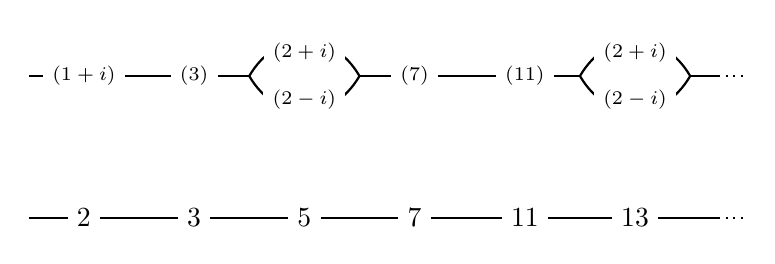
\begin{tikzpicture}[xscale=1.4,yscale=1.2]
    \draw[thick] (0,1.5) to (2,1.5);
    \draw[thick] (2,1.5) .. controls (2.25,2) and (2.75,2) .. (3,1.5);
    \draw[thick] (2,1.5) .. controls (2.25,1) and (2.75,1) .. (3,1.5);
    \draw[thick] (3,1.5) to (5,1.5);
    \draw[thick] (5,1.5) .. controls (5.25,2) and (5.75,2) .. (6,1.5);
    \draw[thick] (5,1.5) .. controls (5.25,1) and (5.75,1) .. (6,1.5);
    \draw[thick] (6,1.5) to (6.25,1.5);
    \draw[thick,dotted] (6.25,1.5) to (6.5,1.5);
    \node[fill=white] at (0.5,1.5) {\scriptsize$(1+i)$};
    \node[fill=white] at (1.5,1.5) {\scriptsize$(3)$};
    \node[fill=white] at (2.5,1.75) {\scriptsize$(2+i)$};
    \node[fill=white] at (2.5,1.25) {\scriptsize$(2-i)$};
    \node[fill=white] at (3.5,1.5) {\scriptsize$(7)$};
    \node[fill=white] at (4.5,1.5) {\scriptsize$(11)$};
    \node[fill=white] at (5.5,1.75) {\scriptsize$(2+i)$};
    \node[fill=white] at (5.5,1.25) {\scriptsize$(2-i)$};
    %
    \draw[thick] (0,0) to (6.25,0);
    \draw[thick,dotted] (6.25,0) to (6.5,0);
    \node[fill=white] at (0.5,0) {$2$};
    \node[fill=white] at (1.5,0) {$3$};
    \node[fill=white] at (2.5,0) {$5$};
    \node[fill=white] at (3.5,0) {$7$};
    \node[fill=white] at (4.5,0) {$11$};
    \node[fill=white] at (5.5,0) {$13$};
  \end{tikzpicture}
\] And, the \(\zeta\) function records the details of how this works!

For more on this covering space philosophy see
\protect\hyperlink{week205}{``Week 205''} and
\protect\hyperlink{week213}{``Week 213''}. This geometrical metaphor
lies behind a lot of the really cool work on number theory.

\textbf{B) The zeta function of a discrete dynamical system.} A
``discrete dynamical system'' consists of a set \(X\) together with a
one-to-one and onto function \[f\colon X \to X\] Here \(X\) is the set
of ``states'' of some physical system, and \(f\) describes one step of
time evolution. For each integer \(n\) we get a function
\[f^n\colon X \to X\] Since the integers are called \(\mathbb{Z}\),
mathematicians would call our discrete dynamical system a
``\(\mathbb{Z}\)-set''.

Whatever you call it, its zeta function is defined to be:
\[\zeta(s) = \prod \frac{1}{1 - |P|^{-s}}\] where \(P\) ranges over all
periodic orbits and \(|P|\) is the \emph{exponential} of the size of
this periodic orbit.

This is like an Euler product formula with the periodic orbits being the
``primes''. Just as every natural number can be uniquely factored into
primes, every discrete dynamical system can be uniquely written as a
disjoint union of periodic orbits. This explains the exponential in the
definition of \(|P|\) above: primes like to multiply, while sizes of
orbits like to add.

One nice thing about this zeta function is that when we take the
disjoint union of two discrete dynamical systems, their zeta functions
multiply. Another nice thing is that the zeta function of a dynamical
system completely describes it up to isomorphism, at least when the set
\(X\) is finite. Decategorification at work!

We can also rewrite this zeta function as a sum:
\[\zeta(s) = \sum |I|^{-s}\] where \(I\) ranges over all formal products
of periodic orbits, and we define
\(|P_1 \ldots P_n| = |P_1| \ldots |P_n|\).

Even better, examples A) and B) overlap. I'll explain how later, but the
key is to associate to any number field and any prime \(p\) a discrete
dynamical system \[f\colon X \to X\] called the ``Frobenius
automorphism''. This gives a zeta function. It works best if we take the
exponential of the size of each periodic orbit using the base \(p\)
instead of base \(e\). Then, if we multiply all these zeta functions,
one for each ordinary prime \(p\), we get the zeta function of our
number field!

\textbf{C) The zeta function of a continuous dynamical system.} Now
suppose \(X\) is some topological space and we have a time evolution map
\[f_t\colon X \to X\] for each real number \(t\). We can define a zeta
function \[\zeta(s) = \prod \frac{1}{1 - |P|^{-s}}\] where \(P\) ranges
over all periodic orbits and \(|P|\) is the exponential of the
``period'' of \(P\) --- meaning the time it takes for points on this
orbit to loop around back to where they started.

A famous example is when we have a Riemannian manifold. A free particle
moving around on such a space will trace out geodesics, giving us a
dynamical system. The analogue of primes are now ``prime geodesics'':
periodic geodesics that loop around just once.

The ``covering space'' philosophy described in example A) can now be
taken literally! If the Riemannian manifold \(M'\) is a covering space
of \(M\), any prime geodesic \(P\) in \(M\) defines a deck
transformation of \(M'\). This transformation acts on the set \(X\) of
prime geodesics sitting over \(P\), so we get a one-to-one and onto map
\[f\colon X \to X\] This is exactly like the ``Frobenius automorphism''
in number theory!

All this is particularly interesting when our manifold is a quotient of
the upper halfplane by a discrete group --- see
\protect\hyperlink{week215}{``Week 215''} for more on this. The reason
is that some of these quotients are related to number theory. So, we get
some direct interactions with example A).

\textbf{D) The zeta function of a graph.} We can take the idea of
``periodic geodesic on a Riemannian manifold'' and vastly simplify it by
looking at closed loops in a graph with finitely many edges and
vertices. We get a \(\zeta\) function
\[\zeta(s) = \prod \frac{1}{1 - |P|^{-s}}\] where \(P\) ranges over all
``prime loops'' in our graph: loops that don't backtrack or loop around
more than once. Now \(|P|\) is the exponential of the length of the
loop.

The ``covering space'' philosophy still applies, since we can define
what it means for a graph \(G'\) to be a covering space of a graph
\(G\). Any prime loop \(P\) in \(G\) defines a deck transformation of
\(G'\). This acts on the set \(X\) of prime loops sitting over \(P\), so
we get a one-to-one and onto map \[f\colon X \to X\] which again
deserves to be called the ``Frobenius automorphism''.

\textbf{E) The zeta function of an affine scheme.} Given a commutative
ring, we can think of it as the ring of functions on some space. The
\(\zeta\) function of the commutative ring then counts the points of
this space.

To make this precise, we cleverly invent a kind of space called an
``affine scheme'', which is secretly \emph{just another name for a
commutative ring!} So, any commutative ring \(R\) gives an affine scheme
called \(\mathrm{Spec}(R)\), purely by our fiendish definition.

If we take a function and evaluate it at a point, we should get a
number. This should give a homomorphism from functions to numbers. But
in algebraic geometry, ``numbers'' can be elements of any field \(k\).
So, let's say the ``\(k\)-points'' of \(\mathrm{Spec}(R)\) are the
homomorphisms from \(R\) to \(k\).

(This is a bit nontraditional, but I really need this here. For a more
traditional alternative, see \protect\hyperlink{week205}{``Week 205''}.)

In particular, for any prime \(p\) we can take \(k\) to be the algebraic
closure of the field with \(p\) elements. Let \(X\) be the set of
\(k\)-points of some affine scheme \(\mathrm{Spec}(R)\). Then comes
something wonderful: if \(x\) is a \(k\)-point, so is \(x^p\), since
``raising to the \(p\)th power'' is an automorphism of \(k\). So, we get
a map \[f\colon X \to X\] sending \(x\) to \(x^p\). This is called the
``Frobenius automorphism''!

Since \(f\) is a discrete dynamical system, we can define its zeta
function as in example B): \[\zeta(s) = \prod \frac{1}{1 - |P|^{-s}}\]
where \(P\) ranges over all periodic orbits, and \(|P|\) is the
exponential of the size of the periodic orbit, defined using the base
\(p\).

So far, this is the zeta function of our affine scheme ``localized at
\(p\)''. If we multiply a bunch of factors like this, one for each
ordinary prime \(p\), we get the zeta function of our affine scheme. For
example, the affine scheme \(\mathrm{Spec}(\mathbb{Z})\) gives the
Riemann zeta function.

In fact, all of example A) fits neatly into this one as a sub-example.
And if you know about schemes that aren't affine --- like projective
varieties, such as elliptic curves and other curves --- you'll see this
definition works for them too.

If you know someone else's definition of the zeta function of a scheme,
it may not look like what I wrote here! But don't panic. The reason is
that people like to express the zeta function of a discrete dynamical
system \(f\colon X \to X\) in terms of the number of fixed points of
\(f^n\). When \(f\) is the Frobenius automorphism, these are usually
called ``points defined over the field with \(p^n\) elements''. So,
you'll see lots of formulas for zeta functions phrased in terms of
these\ldots.

Okay. Enough examples.

There are a lot more, but I think these are the simplest. I hope you see
how all these examples are just different expressions of the same idea.
To go further, I would tell you how there are versions of the Riemann
Hypothesis in all these examples, and also things called
``\(L\)-functions'', and lots of theorems and conjectures concerning
them, too!

It's a wonderful example of the unity of mathematics. But, it's also a
wonderful example of how this unity is obscured by people who zoom in on
their own favorite special case and its particular technical
complexities while never discussing the big picture. You wouldn't
believe how hard it's been for me to figure out what I just told you!
It's like trying to learn English by reading the US legal code, or
learning basic chord progressions by listening to Schoenberg.

If you're just trying to get started, here's one of the more readable
introductions:

\begin{enumerate}
\def\labelenumi{\arabic{enumi})}
\setcounter{enumi}{4}
\tightlist
\item
  Anton Deitman, ``Panorama of zeta functions'', available as
  \href{http://www.arxiv.org/abs/math.NT/0210060}{\texttt{math.NT/0210060}}.
\end{enumerate}

Audrey Terras has a lot of nice slide presentations about the \(\zeta\)
functions and \(L\)-functions of graphs:

\begin{enumerate}
\def\labelenumi{\arabic{enumi})}
\setcounter{enumi}{5}
\item
  Audrey Terras, Artin \(L\)-functions of graph coverings, available at
  \texttt{http://math.ucsd.edu/\textasciitilde{}aterras/artin1.pdf}

  ``More on \(L\)-functions'', available at
  \texttt{http://math.ucsd.edu/\textasciitilde{}aterras/artin2.pdf}
\end{enumerate}

Here's a paper written in broken English but making a very serious
attempt to explain things to the nonexpert:

\begin{enumerate}
\def\labelenumi{\arabic{enumi})}
\setcounter{enumi}{6}
\tightlist
\item
  David Zywina, ``The zeta function of a graph'', available at
  \texttt{http://math.berkeley.edu/\textasciitilde{}zywina/zeta.pdf}
\end{enumerate}

He gives a characterization of graphs whose zeta functions satisfy an
analogue of the Riemann Hypothesis. Strangely, this analogue involves
\emph{poles} of the \(\zeta\) function in the critical strip
\[0 < \Re(s) < 1\] Is this a real difference or the result of some
difference in conventions?

Finally, I should explain some more technical stuff about \(\zeta\)
functions and fixed points, just so I don't forget it. Suppose we have a
discrete dynamical system \[f\colon X \to X\] and let
\[|\mathrm{fix}(f^n)|\] be the number of fixed points of the \(n\)th
iterate of \(f\).

We can define a weird function like this:
\[Z(u) = \exp\left(\sum_{n>0} \frac{|\mathrm{fix}(f^n)| u^n}{n}\right)\]
You'll often see formulas like this running around, especially when
\(f\) is some sort of ``Frobenius automorphism''. Sometimes people even
call these guys zeta functions. But what in the world do they have to do
with zeta functions???

Let's see. Suppose first that \(X\) consists of a single cycle of length
\(k\). Then \(f^n\) has \(k\) fixed points when \(n\) is a multiple of
\(k\), but none otherwise, so: \[
  \begin{aligned}
    Z(u)
    &= \exp\left(\frac{ku^k}{k} + \frac{ku^{2k}}{2k} + \frac{ku^{3k}}{3k} + \ldots\right)
  \\&= \exp\left(u^k + \frac{u^{2k}}{2} + \frac{u^{3k}}{3} + \ldots\right)
  \\&= \exp\left(\ln\frac{1}{1-u^k}\right)
  \\&= \frac{1}{1-u^k}
  \end{aligned}
\] This is starting to look more like the zeta functions we know and
love. It looks even better if we pick some prime number \(p\) and define
\[\zeta(s) = Z(p^{-s})\] Then we get
\[\zeta(s) = \frac{1}{1 - p^{-ks}}\] which is precisely what we'd get
using the definition in example B).

Furthermore, for both that old definition and our new one, the zeta
function of a disjoint union of discrete dynamical systems is the
\emph{product} of the zeta functions of the parts. Since every discrete
dynamical system is a disjoint union of cycles, we conclude that the
definitions \emph{always} agree. In other words,
\[\zeta(s) = Z(p^{-s})\] with
\[Z(u) = \exp\left(\sum_{n>0} \frac{|\mathrm{fix}(f^n)| u^n}{n}\right)\]
is always equal to the zeta function defined in example B).

So, don't let anyone fool you --- there aren't lots of completely
different kinds of zeta functions! There's just a few kinds, and we
could probably boil them down to just ONE kind with some work.

\begin{center}\rule{0.5\linewidth}{0.5pt}\end{center}

\begin{quote}
\emph{Some decades ago I made --- somewhat in jest --- the suggestion
that one should get accepted a non-proliferation treaty of zeta
functions. There was becoming such an overwhelming variety of these
objects.}

--- Atle Selberg
\end{quote}



\hypertarget{week217}{%
\section{May 30, 2005}\label{week217}}

Last week I described lots of different zeta functions, but didn't say
much about what they're good for. This week I'd like to get started on
fixing that problem.

People have made lots of big conjectures related to zeta functions. So
far they've just proved just a few\ldots{} but it's still a big deal.

For example, Andrew Wiles' proof of Fermat's Last Theorem was just a
tiny spin-off of his work on something much bigger called the
Taniyama-Shimura conjecture. Now, personally, I think Fermat's Last
Theorem is a ridiculous thing. The last thing I'd ever want to know is
whether this equation: \[x^n + y^n = z^n\] has nontrivial integer
solutions for \(n > 2\). But the Taniyama-Shimura Conjecture is really
interesting! It's all about the connection between geometry, complex
analysis and arithmetic, and it ties together some big ideas in an
unexpected way. This is how it usually works in number theory: cute but
goofy puzzles get solved as a side-effect of deep and interesting
results related to zeta functions and \(L\)-functions --- sort of like
how the powdered drink ``Tang'' was invented as a spinoff of going to
the moon.

For a good popular book on Fermat's Last Theorem and the
Taniyama-Shimura Conjecture, try:

\begin{enumerate}
\def\labelenumi{\arabic{enumi})}
\tightlist
\item
  Simon Singh, \emph{Fermat's Enigma: The Epic Quest to Solve the
  World's Greatest Mathematical Problem}, Walker, New York, 1997.
\end{enumerate}

Despite the ``world's greatest mathematical problem'' baloney, this book
does a great job of telling the story without drowning the reader in
math.

But you read This Week's Finds because you \emph{want} to be drowned in
math, and I wouldn't want to disappoint you. So, let me list a few of
the big conjectures and theorems related to zeta functions.

Here goes:

\begin{quote}
\textbf{A) The Riemann Hypothesis --- the zeros of the Riemann zeta
function in the critical strip \(0 \leqslant \Re(s) \leqslant 1\)
actually lie on the line \(\Re(s) = 1/2.\)}
\end{quote}

First stated in 1859 by Bernhard Riemann; still open.

This implies a good estimate on the number of primes less than a given
number, as described in \protect\hyperlink{week216}{``Week 216''}.

\begin{quote}
\textbf{B) The Generalized Riemann Hypothesis --- the zeros of any
Dirichlet \(L\)-function that lie in the critical strip actually lie on
the line \(\Re(s) = 1/2.\)}
\end{quote}

Still open, since the Riemann Hypothesis is a special case.

A ``Dirichlet \(L\)-function'' is a function like this:
\[L(\chi,s) = \sum_{n>0} \frac{\chi(n)}{n^s}\] where \(\chi\) is any
``Dirichlet character'', meaning a periodic complex function on the
positive integers such that \[\chi(nm) = \chi(n) \chi(m)\] If we take
\(\chi = 1\) we get back the Riemann zeta function.

Dirichlet used these \(L\)-functions to prove that there are infinitely
many primes equal to \(k \mod n\) as long as \(k\) is relatively prime
to \(n\). The Generalized Riemann Hypothesis would give a good estimate
on the number of such primes less than a given number, just as the
Riemann Hypothesis does for plain old primes.

Erich Hecke established the basic properties of Dirichlet
\(L\)-functions in 1936, including a special symmetry called the
``functional equation'' which Riemann had already shown for his zeta
function. So I bet Hecke must have dreamt of the Generalized Riemann
Hypothesis, even if he didn't dare state it.

\begin{quote}
\textbf{C) The Extended Riemann Hypothesis --- for any number field, the
zeros of its zeta function in the critical strip actually lie on the
line \(\Re(s) = 1/2\).}
\end{quote}

Still open, since the Riemann Hypothesis is a special case.

I described the zeta functions of number fields in
\protect\hyperlink{week216}{``Week 216''}. These are usually called
``Dedekind zeta functions''. Hecke also proved a functional equation for
these back in 1936.

\begin{quote}
\textbf{D) The Grand Riemann Hypothesis --- for any automorphic
\(L\)-function, the zeros in the critical strip actually lie on the line
\(\Re(s) = 1/2\).}
\end{quote}

This is still open too, since it includes A)--C) as special cases!

I don't want to tell you what ``automorphic \(L\)-functions'' are yet.
For now, you can just think of them as grand generalizations of both
Dirichlet \(L\)-functions and zeta functions of number fields.

\begin{quote}
\textbf{E) The Weil Conjectures --- The zeros and poles of the zeta
function of any smooth algebraic variety over a finite field lie on the
lines \(\Re(s) = 1/2, 1, 3/2, \ldots, d/2\) where \(d\) is the dimension
of the variety.} The zeros lie on the lines \(1/2, 3/2, \ldots\) while
the poles lie on the lines \(1, 2, \ldots\). Also: such zeta functions
are quotients of polynomials, they satisfy a functional equation, and a
lot of information about their zeroes and poles can be recovered from
the topology of the corresponding \emph{complex} algebraic varieties.
\end{quote}

First stated in 1949 by Andre Weil; proof completed by Pierre Deligne in
1974 based on much work by Michael Artin, J.-L. Verdier, and especially
Alexander Grothendieck. Grothendieck invented topos theory as part of
the attack on this problem!

\begin{quote}
\textbf{F) The Taniyama-Shimura Conjecture --- every elliptic curve over
the rational numbers is a modular curve.} Or, equivalently: every
\(L\)-function of an elliptic curve is the \(L\)-function of a modular
curve.
\end{quote}

This was first conjectured in 1955 by Yukata Taniyama, who worked on it
with Goro Shimura until committing suicide in 1958. Around 1982 Gerhard
Frey suggested that this conjecture would imply Fermat's Last Theorem;
this was proved in 1986 by Ken Ribet. In 1995 Andrew Wiles and Richard
Taylor proved a big enough special case of the Taniyama-Shimura
Conjecture to get Fermat's Last Theorem. The full conjecture was shown
in 1999 by Breuil, Conrad, Diamond, and Taylor.

I don't want to say what \(L\)-functions of curves are yet\ldots{} but
they are a lot like Dirichlet \(L\)-functions.

\begin{quote}
\textbf{G) The Langlands Conjectures --- any automorphic representation
\(\pi\) of a connected reductive group \(G\), together with a
finite-dimensional representation of its \(L\)-group, gives an
automorphic \(L\)-function \(L(s,\pi)\).} Also: these \(L\)-functions
all satisfy functional equations. Furthermore, they depend functorially
on the group \(G\), its \(L\)-group, and their representations.
\end{quote}

Zounds! Don't worry if this sounds like complete gobbledygook! I only
mention it to show how scary math can get. As Stephen Gelbart once
wrote:

\begin{quote}
The conjectures of Langlands just alluded to amount (roughly) to the
assertion that the other zeta-functions arising in number theory are but
special realizations of these \(L(s,\pi)\).

Herein lies the agony as well as the ecstacy of Langlands' program. To
merely state the conjectures correctly requires much of the machinery of
class field theory, the structure theory of algebraic groups, the
representation theory of real and \(p\)-adic groups, and (at least) the
language of algebraic geometry. In other words, though the promised
rewards are great, the initiation process is forbidding.
\end{quote}

I hope someday I'll understand this stuff well enough to say something
more helpful! Lately I've been catching little glimpses of what it's
about\ldots.

But, right now I think it's best if I talk about the ``functional
equation'' satisfied by the Riemann zeta function, since this gives the
quickest way to see some of the strange things that are going on.

The Riemann zeta function starts out life as a sum:
\[\zeta(s) = 1^{-s} + 2^{-s} + 3^{-s} + 4^{-s} + \ldots\] This only
converges for \(\Re(s) > 1\). It blows up as we approach \(s = 1\),
since then we get the series
\[\frac11 + \frac12 + \frac13 + \frac14 + \ldots\] which diverges.
However, in 1859 Riemann showed that we can analytically continue the
zeta function to the whole complex plane except for this pole at
\(s = 1\).

He also showed that the zeta function has an unexpected symmetry: its
value at any complex number \(s\) is closely related to its value at
\(1-s\). It's not true that \(\zeta(s) = \zeta(1-s)\), but something
similar is true, where we multiply the zeta function by an extra fudge
factor.

To be precise: if we form the function
\[\pi ^{-\frac{s}{2}} \Gamma\left(\frac{s}{2}\right) \zeta(s)\] then
this function is unchanged by the transformation \[s \mapsto 1 - s\]
This symmetry maps the line \[\Re(s) = \frac12\] to itself, and the
Riemann Hypothesis says all the \(\zeta\) zeros in the critical strip
actually lie on this magic line.

This symmetry is called the ``functional equation''. It's the tiny tip
of a peninsula of a vast and mysterious continent which mathematicians
are still struggling to explore. Riemann gave two proofs of this
equation. You can find a precise statement and a version of Riemann's
second proof here:

\begin{enumerate}
\def\labelenumi{\arabic{enumi})}
\setcounter{enumi}{1}
\tightlist
\item
  Daniel Bump, Zeta Function, lecture notes on ``the functional
  equation'' available at
  \texttt{http://math.stanford.edu/\textasciitilde{}bump/zeta.html} and
  \texttt{http://www.maths.ex.ac.uk/\textasciitilde{}mwatkins/zeta/fnleqn.htm}
\end{enumerate}

This proof is a beautiful application of Fourier analysis. Everyone
should learn it, but let me try to sketch the essential idea here.

I will deliberately be VERY rough, and use some simplified nonstandard
definitions, since the precise details have a way of distracting your
eye just as the magician pulls the rabbit out of the hat.

We start with the function \(\zeta(2s)\):
\[1^{-s} + 4^{-s} + 9^{-s} + 25^{-s} + \ldots.\] Then we apply a curious
thing called the ``inverse Mellin transform'', which turns this function
into \[z^1 + z^4 + z^9 + z^{25} + \ldots\] Weird, huh? This is almost
the ``theta function''
\[\theta(t) = \sum_{n\in\mathbb{Z}} e^{\pi i n^2 t}\] Indeed, it's easy
to see that
\[\frac{\theta(t) - 1}{2} = z^1 + z^4 + z^9 + z^25^ + \ldots\] when
\[z = e^{\pi it}\] The theta function transforms in a very simple way
when we replace \(t\) by \(-1/t\), as one can show using Fourier
analysis.

Unravelling the consequences, this implies that the zeta function
transforms in a simple way when we replace \(s\) by \(1-s\). You have to
go through the calculation to see precisely how this works\ldots{} but
the basic idea is: a symmetry in the theta function yields a symmetry in
the zeta function.

Hmm, I'm not sure that explained anything! But I hope at least the
mystery is more evident now. A bunch of weird tricks, and then
\emph{presto} --- the functional equation! To make progress on
understanding the Riemann Hypothesis and its descendants, we need to get
what's going on here.

I feel I \emph{do} get the inverse Mellin transform; I'll say more about
that later. But for now, note that the theta function transforms in a
simple way, not just when we do this: \[t \mapsto -\frac{1}{t}\] but
also when we do this: \[t \mapsto t + 2\] Indeed, it doesn't change at
all when we add \(2\) to \(t\), since \(e^{2\pi i} = 1\).

Now, the maps \[t \mapsto -\frac1t\] and \[t \mapsto t + 1\] generate
the group of all maps \[t \mapsto \frac{at+b}{ct+d}\] where \(a,b,c,d\)
form a \(2\times2\) matrix of integers with determinant \(1\). These
maps form a group called \(\mathrm{PSL}(2,\mathbb{Z})\), or the
``modular group''.

A function that transforms simply under this group and doesn't blow up
in nasty ways is called a ``modular form''. In
\protect\hyperlink{week197}{``Week 197''} I gave the precise definition
of what counts as transforming simply and not blowing up in nasty ways.
I also explained how modular forms are related to elliptic curves and
string theory. So, please either reread
\protect\hyperlink{week197}{``Week 197''} or take my word for it:
modular forms are cool!

The theta function is almost a modular form, but not quite. It doesn't
blow up in nasty ways. However, it only transforms simply under a
subgroup of \(\mathrm{PSL}(2,\mathbb{Z})\), namely that generated by
\[t \mapsto -\frac1t\] and \[t \mapsto t + 2\] So, the theta function
isn't a full-fledged modular form. But since it comes close, we call it
an ``automorphic form''.

Indeed, for any discrete subgroup \(G\) of
\(\mathrm{PSL}(2,\mathbb{Z})\), functions that transform nicely under
\(G\) and don't blow up in nasty ways are called ``automorphic forms''
for \(G\). They act a lot like modular forms, and people know vast
amounts about them. It's the power of automorphic forms that makes
number theory what it is today!

We can summarize everything so far in this slogan:

\begin{quote}
THE FUNCTIONAL EQUATION FOR THE RIEMANN ZETA FUNCTION SAYS:\\
``THE THETA FUNCTION IS AN AUTOMORPHIC FORM''
\end{quote}

But before you start printing out bumper stickers, I should
explain\ldots.

The point of this slogan is this. We \emph{thought} we were interested
in the Riemann zeta function for its own sake, or what it could tell us
about prime numbers. But with the wisdom of hindsight, the first thing
we should do is hit this function with the inverse Mellin transform and
repackage all its information into an automorphic form --- the theta
function.

\(\zeta\) is dead, long live \(\theta\)!

The Riemann zeta function is just like all the fancier zeta functions
and \(L\)-functions in this respect. The fact that they satisfy a
``functional equation'' is just another way of saying their inverse
Mellin transforms are automorphic forms\ldots{} and it's these
automorphic forms that exhibit the deeper aspects of what's going on.

Now let me say a little bit about the inverse Mellin transform.

Ignoring various fudge factors, the inverse Mellin transform is
basically just the linear map that sends any function of \(s\) like
this: \[n^{-s}\] to this function of \(z\): \[z^n\] In other words, it
basically just turns things upside down, replacing the base by the
exponent and vice versa. The minus sign is just a matter of convention;
don't worry about that too much.

So, the inverse Mellin transform basically sends any function like this,
called a ``Dirichlet series'':
\[a_1 1^{-s} + a_2 2^{-s} + a_3 3^{-s} + a_4 4^{-s} + \ldots\] to this
function, called a ``Taylor series'':
\[a_1 z^1 + a_2 z^2 + a_3 z^3 + a_4 z^4 + \ldots\] Now, why would we
want to do this?

The reason is that multiplying Taylor series is closely related to
\emph{addition} of natural numbers: \[z^n z^m = z^{n+m}\] while
multiplying Dirichlet series is closely related to \emph{multiplication}
of natural numbers: \[n^{-s} m^{-s} = (nm)^{-s}\] The Mellin transform
(and its inverse) are how we switch between these two pleasant setups!

Indeed, it's all about algebra --- at least at first. We can add natural
numbers and multiply them, so \(\mathbb{N}\) becomes a monoid in two
ways. A ``monoid'', recall, is a set with a binary associative product
and unit. So, we have two closely related monoids: \[(\mathbb{N},+,0)\]
and \[(\mathbb{N},\times,1)\] Given a monoid, we can form something
called its ``monoid algebra'' by taking formal complex linear
combinations of monoid elements. We multiply these in the obvious way,
using the product in our monoid.

If we take the monoid algebra of \((\mathbb{N},+,0)\), we get the
algebra of Taylor series! If we take the monoid algebra of
\((\mathbb{N},\times,1)\), we get the algebra of Dirichlet series!

(Actually, this is only true if we allow ourselves to use
\emph{infinite} linear combinations of monoid elements in our monoid
algebra. So, let's do that. If we used finite linear combinations, as
people often do, \((\mathbb{N},+,0)\) would give us the algebra of
polynomials, while \((\mathbb{N},\times,0)\) would give us the algebra
of ``Dirichlet polynomials''.)

Of course, algebraically we can combine these structures.
\((\mathbb{N},+,\times,0,1)\) is a rig, and by taking formal complex
linear combinations of natural numbers we get a ``rig algebra'' with two
products: the usual product of Taylor series, and the usual product of
Dirichlet series. They're compatible, too, since one distributes over
the other. They both distribute over addition.

However, if we're trying to get an algebra of functions on the complex
plane, with pointwise multiplication as the product, we need to make up
our mind: either Taylor series or Dirichlet series! We then need the
Mellin transform to translate between the two.

So, what seems to be going on is that people take a puzzle, like

\begin{quote}
``what is the sum of the squares of the divisors of \(n\)?''
\end{quote}

or

\begin{quote}
``how many ideals of order \(n\) are there in this number field?''
\end{quote}

and they call the answer \(a_n\).

Then they encode this sequence as either a Dirichlet series:
\[a_1 1^{-s} + a_2 2^{-s} + a_3 3^{-s} + a_4 4^{-s} + \ldots\] or a
Taylor series: \[a_1 z^1 + a_2 z^2 + a_3 z^3 + a_4 z^4 + \ldots\] The
first format is nice because it gets along well with multiplication of
natural numbers. For example, in the puzzle about ideals, every ideal is
a product of prime ideals, and its norm is the product of the norms of
those prime ideals\ldots{} so our Dirichlet series will have an Euler
product formula.

The second format is nice \emph{if} our Taylor series is an automorphic
form. This will happen precisely when our Dirichlet series satisfies a
functional equation.

(For experts: I'm ignoring some fudge factors involving the gamma
function.)

I still need to say more about \emph{which} puzzles give automorphic
forms, what it really means when they \emph{do}. But, not this week! I'm
tired, and I bet you are too.

For now, let me just give some references. There's a vast amount of
material on all these subjects, and I've already referred to lots of it.
But right now I want to focus on stuff that's free online, especially
stuff that's readable by anyone with a solid math background --- not
journal articles for experts, but not fluff, either.

Here's some information on the Riemann Hypothesis provided by the Clay
Mathematics Institute, which is offering a million dollars for its
solution:

\begin{enumerate}
\def\labelenumi{\arabic{enumi})}
\setcounter{enumi}{2}
\tightlist
\item
  Clay Mathematics Institute, ``Problems of the Millennium: the Riemann
  Hypothesis'', \texttt{http://www.claymath.org/millennium/}
\end{enumerate}

The official problem description by Enrico Bombieri talks about evidence
for the Riemann Hypothesis, including the Weil Conjectures. The article
by Peter Sarnak describes generalizations leading up to the Grand
Riemann Hypothesis. In particular, he gives a super-rapid introduction
to automorphic \(L\)-functions.

Here's a nice webpage that sketches Wiles and Taylor's proof of Fermat's
last theorem:

\begin{enumerate}
\def\labelenumi{\arabic{enumi})}
\setcounter{enumi}{3}
\tightlist
\item
  Charles Daney, ``The Mathematics of Fermat's Last Theorem'',
  \texttt{http://www.mbay.net/\textasciitilde{}cgd/flt/fltmain.htm}
\end{enumerate}

I like the quick introductions to ``Elliptic curves and elliptic
functions'', ``Elliptic curves and modular functions'', ``Zeta and
\(L\)-functions'', and ``Galois Representations'' --- they're neither
too detailed nor too vague, at least for me.

Here's a nice little intro to the Weil Conjectures:

\begin{enumerate}
\def\labelenumi{\arabic{enumi})}
\setcounter{enumi}{4}
\tightlist
\item
  Runar Ile, ``Introduction to the Weil Conjectures'',
  \texttt{http://folk.uio.no/\textasciitilde{}ile/WeilA4.pdf}
\end{enumerate}

James Milne goes a lot deeper --- his course notes on etale cohomology
include a proof of the Weil Conjectures:

\begin{enumerate}
\def\labelenumi{\arabic{enumi})}
\setcounter{enumi}{5}
\tightlist
\item
  James Milne, ``Lectures on Etale Cohomology'',
  \texttt{http://www.jmilne.org/math/CourseNotes/math732.html}
\end{enumerate}

while his course notes on elliptic curves sketch the proof of Fermat's
Last Theorem:

\begin{enumerate}
\def\labelenumi{\arabic{enumi})}
\setcounter{enumi}{6}
\tightlist
\item
  James Milne, ``Elliptic Curves'',
  \texttt{http://www.jmilne.org/math/CourseNotes/math679.html}
\end{enumerate}

Here's a nice history of what I've been calling the Taniyama-Shimura
Conjecture, which explains why some people call it the
Taniyama-Shimura-Weil conjecture, or other things:

\begin{enumerate}
\def\labelenumi{\arabic{enumi})}
\setcounter{enumi}{7}
\tightlist
\item
  Serge Lang, ``Some history of the Shimura-Taniyama Conjecture'',
  \emph{AMS Notices} \textbf{42} (November 1995), 1301--1307. Available
  at \texttt{http://www.ams.org/notices/199511/forum.pdf}
\end{enumerate}

Here's a quick introduction to the proof of this conjecture, whatever
it's called:

\begin{enumerate}
\def\labelenumi{\arabic{enumi})}
\setcounter{enumi}{8}
\tightlist
\item
  Henri Darmon, ``A proof of the full Shimura-Taniyama-Weil Conjecture
  is announced'', \emph{AMS Notices} \textbf{46} (December 1999),
  1397--1401. Available at
  \texttt{http://www.ams.org/notices/199911/comm-darmon.pdf}
\end{enumerate}

I won't give any references to the Langlands Conjectures, since I hope
to talk a lot more about those some other time.

And, I hope to keep on understanding this stuff better and better!

I thank James Borger and Kevin Buzzard for help with this issue of This
Week's Finds.

\begin{center}\rule{0.5\linewidth}{0.5pt}\end{center}

\textbf{Addendum:} Here's part of an email exchange I had with Kevin
Buzzard of Imperial College after he read this Week's Finds:

I wrote:

\begin{quote}
What I \emph{REALLY} want to know is: what combinatorial properties of
an integer sequence an are we being told when we're told that the
Dirichlet series \[\sum_n a^n n^{-s}\] comes from an automorphic form?
\end{quote}

He replied:

\begin{quote}
Yeah, that's a really key question. I'm not sure that there is an
elementary answer. Here is another question: given a sequence of complex
numbers \(a_1, a_2,\ldots,a_n,\ldots\), with \[a_n = \mathcal{O}(n^r),\]
what is a neat easy-to-understand property of this sequence which
implies (or is implied by, or is equivalent to) the statement that
\[\sum \frac{a_n}{n^s}\] has analytic (or meromorphic) continuation
beyond \(\Re(s)>r\)? Maybe even this is hard---or maybe there is no such
elementary criterion.

\begin{quote}
I'll be happy to assume for starters that an is multiplicative.
\end{quote}

This might not ``logically speaking'' be necessary, but on the other
hand probably the most interesting cases have this property. Here is an
example. Take a sequence of complex numbers \(a_1, a_2, \ldots\) which
is periodic with prime period \(p\) (primality probably isn't necessary
but it simplifies the combinatorics). Then the associated \(L\)-function
\[\sum \frac{a_n}{n^s}\] has meromorphic continuation with at worst a
simple pole at \(s=1\) and no other poles, and one could even argue that
the \(a_i\) ``came from an automorphic form''.

On the other hand, this is not the kind of automorphic form that people
usually think about because it's not an eigenform. What is happening is
that ``there are enough Dirichlet characters'': consider the trivial
character \(\chi(n)=1\) for all \(n\), and then the \(p-1\) Dirichlet
characters of level \(p\), those defined by group homomorphisms
\[\chi\colon (\mathbb{Z}/p\mathbb{Z})^* \to \mathbb{C}^*\] and extended
to functions on \(\mathbb{Z}\) by \(\chi(n)=0\) for \(n\) a multiple of
\(p\). These \(p\) functions on \(\mathbb{Z}\) form a basis of the
vector space of periodic functions on \(\mathbb{Z}\) with period \(p\).

The Dirichlet characters give automorphic forms, but automorphic forms
are a vector space so you can add them together and get an automorphic
form for any periodic function. However the Dirichlet characters are the
most interesting such forms because these are the ones which are
eigenforms. The eigenforms give multiplicative \(a_n\), but it's
certainly not true in general that a periodic function is
multiplicative.

But I can't really enlighten you much further. I know that the
\(L\)-function of an automorphic form has meromorphic continuation and
that we understand the poles (but we only conjecturally understand the
zeroes). However if someone put some \(a_n\) in front of me I would
demand that they told me where the \(a_n\) had come from before I put my
money on whether there was an automorphic form.

The example where I actually proved something was in the case where the
\(a_n\) came from a finite-dimensional complex representation of
\(\mathrm{Gal}(K/\mathbb{Q})\) with \(K\) a number field, Galois over
\(\mathbb{Q}\). (In fact my only contribution was in the
\(2\)-dimensional case, the \(1\)-dimensional case having been
understood for some time.) The \(a_n\) are then related to traces of the
representation. Artin conjectured in the 1930s that \[\sum a_n/n^s\]
should have analytic continuation to all of the complex plane if the
representation was irreducible and not the trivial \(1\)-dimensional
representation. Langlands conjectured much later that the \(a_n\) should
come from an automorphic form, and we knew by then that Langlands'
conjecture implied Artin's. But none of the analytic guys know how to
prove Artin's conjecture without essentially deducing it from
Langlands'! I did something with some other Brits in the
\(2\)-dimensional case. Ironically, to deduce our analytic continuation
results, we proved some \(p\)-adic analytic continuation results first
:-) We constructed a modular form using \(p\)-adic techniques (and all
of Wiles' machinery).

\begin{quote}
I get the feeling that nobody knows the answer, except perhaps for
specific cases like modular forms, where we know they're all linear
combinations of products of Eisenstein series, so that an is built out
of sequences like \(\sigma_k(n)\) --- sums of \(k\)th powers of
divisors.
\end{quote}

But unfortunately this is only true for ``level 1'' modular forms: you
can build all modular forms of level 1 from the Eisenstein series
\(\mathrm{E}_4\) and \(\mathrm{E}_6\). There is no neat analogous result
for modular forms for the group \(\Gamma_0(N)\) for general \(N\). In
particular you will never see the \(a_n\) for an elliptic curve built up
from Eisenstein series in this way :-(

\begin{quote}
What I'd like is a really ``conceptual'' answer\ldots{} or else for
someone to admit that nobody knows such an answer yet.
\end{quote}

I think I will freely admit that, although that's just a personal
opinion.

\begin{center}\rule{0.5\linewidth}{0.5pt}\end{center}

Here is why Dirichlet characters are the same as \(1\)-dimensional
complex representations of
\(\mathrm{Gal}(\overline{\mathbb{Q}}/\mathbb{Q})\). It's called the
Kronecker-Weber theorem, it pre-dates class field theory (although it is
now a special case), and you can \emph{just about} prove it at the end
of an introductory undergraduate course on number fields, as the last
starred question on the example sheet, and only for people that have
done the Galois theory course too. Let \(K\) be a number field and
assume \(K\) is Galois over \(\mathbb{Q}\) (equivalently, that there is
a polynomial \(f\) with rational coefficients such that \(K\) is the
smallest subfield of the complex numbers containing all the roots of
\(f\); \(K\) is called the ``splitting field'' of \(f\)).

Then \(K\) has a Galois group \(\mathrm{Gal}(K/\mathbb{Q})\), which is
the field automorphisms of \(K\) that fix \(\mathbb{Q}\). Say \(f\) has
degree \(n\) and \(n\) roots \(z_1, z_2, \ldots , z_n\). Then any
automorphism of \(K\) fixes \(f\), so it permutes the roots of \(f\). So
we get an embedding \[\mathrm{Gal}(K/\mathbb{Q}) \to S_n\] where \(S_n\)
is the symmetric group on the set \(z_1, z_2, \ldots , z_n\). Then any
automorphism of \(K\) fixes \(f\), so it permutes the roots of \(f\). So
we get an embedding

``Generically'' this map is an isomorphism. But certainly not always ---
if there are subtle relations amongst the \(z_i\) with rational
coefficients then these subtle relations must also be preserved by the
Galois group. One of my favourite examples is the equation \(x^4-2\).
This is an irreducible polynomial of degree 4, the four roots are \(z\),
\(iz\), \(-z\) and \(-iz\) where \(z\) is the real 4th root of \(2\) and
\(i\) is \(\sqrt{-1}\). But \(z+(-z) = 0\), so if \(K\) is the field
generated by these roots and \(\sigma\) is an automorphism of \(K\) then
\(\sigma(z)+\sigma(-z)\) will also be zero, and the Galois group cannot
possibly be all of \(S_4\). In fact one can check that the Galois group
is \(D_8\), the dihedral group with 8 elements (the four roots form a
square in the complex plane and it's the symmetries of this square).

So there's Galois theory. Now here's a question: can we classify all the
number fields \(K\), Galois over \(\mathbb{Q}\), with
\(\mathrm{Gal}(K/\mathbb{Q})\) an abelian group?

Here are some examples: \(K=\mathbb{Q}(\sqrt{d})\), the splitting field
of \(x^2-d\). If \(d\) is the square of a rational then \(K=\mathbb{Q}\)
and if not then it's an extension of degree 2, with Galois group \(S_2\)
which is abelian.

The splitting field of \(x^n-1\), called the \(n\)th cyclotomic field,
also turns out to have abelian Galois group; if \(z = \exp(2\pi in)\)
then any automorphism of \(K\) must send \(z\) to another \(n\)th root
of unity and furthermore the \(n\)th root of unity must have ``exact
order \(n\)'', i.e. its \(n\)th power must be 1 but none of its \(m\)th
powers can be 1 for \(0 < m < n\). So \(z\) must get sent to \(z^a\)
with \(0 < a < n\) coprime to \(n\). This gives us an injection
\[\mathrm{Gal}(K/\mathbb{Q}) \to (\mathbb{Z}/n\mathbb{Z})^*,\] where
\((\mathbb{Z}/n\mathbb{Z})^*\) is the units in the ring
\(\mathbb{Z}/n\mathbb{Z}\) (send \(\sigma\) to \(a\)), and it's tricky
but true that this is in fact an isomorphism (use the fundamental
theorem of Galois theory, and cyclotomic polynomials, or try and get a
``trick'' proof that uses as little of this as possible, but it's still
some work). In any case \(\mathrm{Gal}(K/\mathbb{Q})\) is certainly
abelian.

Next example: any subfield of any previous example, because this is how
Galois theory works: if \(K\) contains \(L\) contains \(\mathbb{Q}\),
and both \(K\) and \(L\) are Galois over \(Q\), then the obvious
restriction map
\(\mathrm{Gal}(K/\mathbb{Q}) \to \mathrm{Gal}(L/\mathbb{Q})\) is a
surjection.

So we now have quite a general example of a number field \(K\) with
\(\mathrm{Gal}(K/\mathbb{Q})\) abelian: any subfield of a cyclotomic
field. The hard theorem (not really too hard, but quite messy) is that
the converse is true: \(\mathrm{Gal}(K/\mathbb{Q})\) abelian implies
that \(K\) is contained within a cyclotomic field. For example
\(\mathbb{Q}(\sqrt{5})\) is in the 5th cyclotomic field because
\(\cos(72^\circ) = (\sqrt{5}-1)/4\).

Any Dirichlet character gives a group homomorphism
\[(\mathbb{Z}/n\mathbb{Z})^* \to \mathbb{C}^*,\] so a map
\[\mathrm{Gal}(K_n/\mathbb{Q}) \to \mathbb{C}^*,\] with \(K_n\) the
\(n\)th cyclotomic field, so a continuous group homomorphism
\[\mathrm{Gal}(\overline{\mathbb{Q}}/\mathbb{Q}) \to \mathbb{C}^*.\]
Conversely any continuous group homomorphism
\[\mathrm{Gal}(\overline{\mathbb{Q}}/\mathbb{Q}) \to \mathbb{C}^*\]
factors through a compact discrete quotient of
\(\mathrm{Gal}(\overline{\mathbb{Q}}/\mathbb{Q})\), which is just
\(\mathrm{Gal}(K/\mathbb{Q})\) for some number field \(K\), and we get
an injection \[\mathrm{Gal}(K/\mathbb{Q}) \to \mathbb{C}^*,\] so
\(\mathrm{Gal}(K/\mathbb{Q})\) is abelian, so \(K\) is contained in a
\(K^n\) for some \(n\), so we get a map
\[\mathrm{Gal}(K_n/\mathbb{Q}) \to \mathbb{C}^*\] so it's a Dirichlet
character.

Amazingly it might have been Langlands who really sold this ``duality''
point, 100 years after it was understood: people always used to state
Kronecker--Weber as ``any abelian number field is contained in a cyclo
field'' rather than the dual ``any \(1\)-dimensional rep of
\(\mathrm{Gal}(\overline{\mathbb{Q}}/\mathbb{Q})\) comes from a
Dirichlet character''. It was perhaps Langlands who realised that the
correct generalisation of this statement was ``any \(n\)-dimensional rep
of \(\mathrm{Gal}(\overline{\mathbb{Q}}/\mathbb{Q})\) comes from an
automorphic form'', rather than a statement about non-abelian extensions
of \(\mathrm{Gal}(\overline{\mathbb{Q}}/\mathbb{Q})\). Perhaps you will
like the reason that people find the representation-theoretic approach
appealing: I have been talking about number fields as subfields of the
complexes, but really a number field is an abstract object which is a
field and happens to have finite dimension over \(\mathbb{Q}\), but it
does not have a preferred embedding into the complexes. As a result of
this sort of thinking, one realises that \(\overline{\mathbb{Q}}\) is
unique, but only up to highly non-unique isomorphism, and hence
\(\mathrm{Gal}(\overline{\mathbb{Q}}/\mathbb{Q})\) is a ``group only
defined up to inner automorphism''! Hence it almost makes no sense to
study this group---we cannot make any serious sense of an element of
this group, because it's only the conjugacy classes that are
well-defined. Hence we should study the representations of the group on
abstract vector spaces (i.e.~ones without preferred bases), because
these are well-defined up to isomorphism. The reason there was so much
mileage in the abelian case was that this subtlety goes away: an abelian
group up to inner automorphism is an abelian group.

\begin{center}\rule{0.5\linewidth}{0.5pt}\end{center}

I know some facts about the sequence \(a_n\) coming from, say, an
elliptic curve over the rationals, but the killer, and one that is
really hard to ``read off'' from the \(a_n\), is that the \(a_n\) are
related to the traces of Frobenius elements on a \(2\)-dimensional
\(p\)-adic Galois representation (the Tate module of the curve). The
moment I see a Galois representation I think that this must be something
to do with automorphic forms, so that's why I believe that the
\(L\)-function of an elliptic curve should come from a modular form. And
it does! On the other hand, if you give me any finite set of primes
\(p\), and any integers \(a_p\) with \(p\) running through the set, such
that \(|a_p|^2\leqslant 4p\), then I can concoct an elliptic curve with
these \(a_p\), so at the very least one has to look at infinitely many
of the \(a_n\) before one can begin to guess whether the \(a_n\) come
from an automorphic form.

Kevin
\end{quote}

\begin{center}\rule{0.5\linewidth}{0.5pt}\end{center}

\begin{quote}
\emph{If I were to awaken after having slept for a thousand years, my
first question would be: ``Has the Riemann hypothesis been proven?''}

--- David Hilbert
\end{quote}



\hypertarget{week218}{%
\section{June 5, 2005}\label{week218}}

Classes are over! Summer is here! Now I can finally get some work done!
I'll be travelling to Sydney, Canberra, Beijing, Chengdu and Calgary,
but mainly I want to finish writing some papers.

First, though, I need to recover from a hard quarter. I need to goof off
a bit! I spent most of yesterday lying in bed reading. Now I want to
talk some more about number theory.

Let's see, where were we? I had just begun to introduce the theme of
\(L\)-functions and their corresponding automorphic forms. My ultimate
goal is to understand the Langlands Conjectures well enough to give a
decent explanation of what they say. Instead of simply stating them, I'd
like to really make them plausible, and this will take quite an
elaborate warmup. So, this Week I want to talk about some background.

Actually, this reminds me of something Feynman wrote: whenever he worked
on a problem, he needed the feeling he had some ``inside track'' ---
some insight or trick up his sleeve that nobody else had. Most of us
will never be as good as Feynman at choosing an ``inside track''. But I
think we all need one to convert what would otherwise be a dutiful and
doomed struggle to catch up with the experts into something more hopeful
and exciting: a personal quest!

For anyone with a physics background, a good ``inside track'' on almost
any math problem is to convert it into some kind of crazy physics
problem. It doesn't need to be realistic physics, just anything you can
apply physics intuition to! This is part of why string theorists have
been so successful in cracking math problems. It also underlies Alain
Connes' attempt to prove the Riemann Hypothesis:

\begin{enumerate}
\def\labelenumi{\arabic{enumi})}
\item
  Alain Connes, ``Noncommutative Geometry, Trace Formulas, and the Zeros
  of the Riemann Zeta Function''. Ohio State course notes and videos at
  \texttt{http://www.math.ohio-state.edu/lectures/connes/Connes.html}

  Alain Connes, ``Trace formula in noncommutative geometry and the zeros
  of the Riemann zeta function'', available as
  \href{http://www.arxiv.org/abs/math.NT/9811068}{\texttt{math.NT/9811068}}.
\item
  Mathilde Marcolli, ``Noncommutative geometry and number theory'',
  available at
  \texttt{http://www.math.fsu.edu/\textasciitilde{}marcolli/ncgntE.pdf}
\end{enumerate}

Of course, Connes also has another ``inside track'', namely his theory
of noncommutative geometry.

By the way: a number theorist I know says he thinks Connes has
essentially proved the Riemann Hypothesis, in the same way that Riemann
``essentially'' proved the Prime Number Theorem. Namely, he has reduced
it to some facts that seem obviously true! Of course, it took about 40
years, from 1859 to 1896, for Riemann's plan to be fulfilled by Hadamard
and De La Vallee Poussin. So, even if Connes' insights are correct, it
may be a while before the Riemann Hypothesis is actually proved.

For anyone with a background in geometry, a good ``inside track'' on
almost any math problem is to convert it into a geometry problem. In the
case of number theory this trick is old news, but still very much worth
knowing. It's based on an analogy which I began discussing in
\protect\hyperlink{week198}{``Week 198''}.

The analogy starts out like this:

\begin{longtable}[]{@{}ll@{}}
\toprule
\begin{minipage}[b]{0.42\columnwidth}\raggedright
Number theory\strut
\end{minipage} & \begin{minipage}[b]{0.52\columnwidth}\raggedright
Complex geometry\strut
\end{minipage}\tabularnewline
\midrule
\endhead
\begin{minipage}[t]{0.42\columnwidth}\raggedright
Integers, \(\mathbb{Z}\)\strut
\end{minipage} & \begin{minipage}[t]{0.52\columnwidth}\raggedright
Polynomial functions on the complex plane, \(\mathbb{C}[z]\)\strut
\end{minipage}\tabularnewline
\begin{minipage}[t]{0.42\columnwidth}\raggedright
Rational numbers, \(\mathbb{Q}\)\strut
\end{minipage} & \begin{minipage}[t]{0.52\columnwidth}\raggedright
Rational functions on the complex plane, \(\mathbb{C}(z)\)\strut
\end{minipage}\tabularnewline
\begin{minipage}[t]{0.42\columnwidth}\raggedright
Prime numbers, \(\mathbb{P}\)\strut
\end{minipage} & \begin{minipage}[t]{0.52\columnwidth}\raggedright
Points in the complex plane, \(\mathbb{C}\)\strut
\end{minipage}\tabularnewline
\bottomrule
\end{longtable}

Why is this analogy good? Well, for starters:

\begin{quote}
Every rational number is a ratio of integers.\\

Every rational function is a ratio of polynomials.
\end{quote}

Better yet:

\begin{quote}
Every integer can be uniquely factored into primes\\
(modulo invertible integers, namely \(+1\) and \(-1\)).\\

Every complex polynomial can be uniquely factored into linear
polynomials\\
(modulo invertible polynomials, namely nonzero constants).
\end{quote}

There's one linear polynomial \(z-a\) for each point \(a\) in the
complex plane, so \emph{primes} are like \emph{points} in the complex
plane.

We can make this precise using the concept of ``spectrum'', which I
defined in \protect\hyperlink{week199}{``Week 199''}. Ignoring a certain
little sublety which is discussed there:

\begin{quote}
The spectrum of \(\mathbb{Z}\) is the set of prime numbers.\\

The spectrum of \(\mathbb{C}[z]\) is the complex plane.
\end{quote}

This way of thinking lets us treat the spectrum of any algebraic
extension of the integers, like the Gaussian integers, as a ``covering
space'' of the set of prime numbers. I've already drawn this picture: \[
  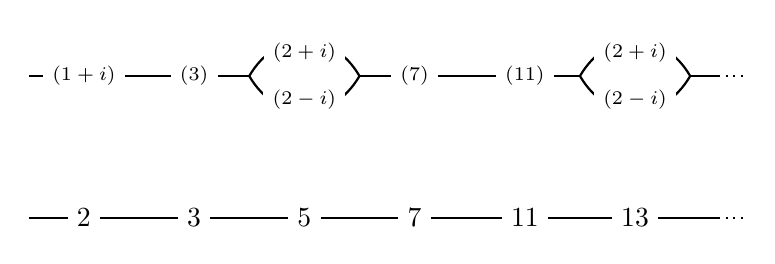
\begin{tikzpicture}[xscale=1.4,yscale=1.2]
    \draw[thick] (0,1.5) to (2,1.5);
    \draw[thick] (2,1.5) .. controls (2.25,2) and (2.75,2) .. (3,1.5);
    \draw[thick] (2,1.5) .. controls (2.25,1) and (2.75,1) .. (3,1.5);
    \draw[thick] (3,1.5) to (5,1.5);
    \draw[thick] (5,1.5) .. controls (5.25,2) and (5.75,2) .. (6,1.5);
    \draw[thick] (5,1.5) .. controls (5.25,1) and (5.75,1) .. (6,1.5);
    \draw[thick] (6,1.5) to (6.25,1.5);
    \draw[thick,dotted] (6.25,1.5) to (6.5,1.5);
    \node[fill=white] at (0.5,1.5) {\scriptsize$(1+i)$};
    \node[fill=white] at (1.5,1.5) {\scriptsize$(3)$};
    \node[fill=white] at (2.5,1.75) {\scriptsize$(2+i)$};
    \node[fill=white] at (2.5,1.25) {\scriptsize$(2-i)$};
    \node[fill=white] at (3.5,1.5) {\scriptsize$(7)$};
    \node[fill=white] at (4.5,1.5) {\scriptsize$(11)$};
    \node[fill=white] at (5.5,1.75) {\scriptsize$(2+i)$};
    \node[fill=white] at (5.5,1.25) {\scriptsize$(2-i)$};
    %
    \draw[thick] (0,0) to (6.25,0);
    \draw[thick,dotted] (6.25,0) to (6.5,0);
    \node[fill=white] at (0.5,0) {$2$};
    \node[fill=white] at (1.5,0) {$3$};
    \node[fill=white] at (2.5,0) {$5$};
    \node[fill=white] at (3.5,0) {$7$};
    \node[fill=white] at (4.5,0) {$11$};
    \node[fill=white] at (5.5,0) {$13$};
  \end{tikzpicture}
\] But, now I'm saying that the ``line'' down below really acts like the
complex \emph{plane}. Taking this strange idea seriously leads to all
sorts of amazing insights.

For example, if you poke a hole in this ``plane'' at some prime, there's
something like a little \emph{loop} that goes around this hole! In other
words, there's a sense in which the spectrum of \(\mathbb{Z}\) has a
nontrivial ``fundamental group'', which contains an element for each
prime. Technically this group is called the Galois group
\(\mathrm{Gal}(\overline{\mathbb{Q}}/\mathbb{Q})\), and we get an
element in it for each prime, called the ``Frobenius automorphism'' for
that prime.

Another cool thing is that we can study integers ``locally'', one prime
at a time, just like we study complex functions locally. We can analyze
functions at a point using Taylor series and Laurent series. And, we can
stretch our analogy to include these concepts:

\begin{longtable}[]{@{}ll@{}}
\toprule
\begin{minipage}[b]{0.42\columnwidth}\raggedright
Number theory\strut
\end{minipage} & \begin{minipage}[b]{0.52\columnwidth}\raggedright
Complex geometry\strut
\end{minipage}\tabularnewline
\midrule
\endhead
\begin{minipage}[t]{0.42\columnwidth}\raggedright
Integers, \(\mathbb{Z}\)\strut
\end{minipage} & \begin{minipage}[t]{0.52\columnwidth}\raggedright
Polynomial functions on the complex plane, \(\mathbb{C}[z]\)\strut
\end{minipage}\tabularnewline
\begin{minipage}[t]{0.42\columnwidth}\raggedright
Rational numbers, \(\mathbb{Q}\)\strut
\end{minipage} & \begin{minipage}[t]{0.52\columnwidth}\raggedright
Rational functions on the complex plane, \(\mathbb{C}(z)\)\strut
\end{minipage}\tabularnewline
\begin{minipage}[t]{0.42\columnwidth}\raggedright
Prime numbers, \(\mathbb{P}\)\strut
\end{minipage} & \begin{minipage}[t]{0.52\columnwidth}\raggedright
Points in the complex plane, \(\mathbb{C}\)\strut
\end{minipage}\tabularnewline
\begin{minipage}[t]{0.42\columnwidth}\raggedright
Integers \(\mod p^n\), \(\mathbb{Z}/p^n\)\strut
\end{minipage} & \begin{minipage}[t]{0.52\columnwidth}\raggedright
\((n-1)\)st-order Taylor series, \(\mathbb{C}[z]/(z-a)^n\)\strut
\end{minipage}\tabularnewline
\begin{minipage}[t]{0.42\columnwidth}\raggedright
\(p\)-adic integers, \(\mathbb{Z}_p\)\strut
\end{minipage} & \begin{minipage}[t]{0.52\columnwidth}\raggedright
Taylor series, \(\mathbb{C}[[z-a]]\)\strut
\end{minipage}\tabularnewline
\begin{minipage}[t]{0.42\columnwidth}\raggedright
\(p\)-adic numbers, \(\mathbb{Q}_p\)\strut
\end{minipage} & \begin{minipage}[t]{0.52\columnwidth}\raggedright
Laurent series, \(\mathbb{C}((z-a))\)\strut
\end{minipage}\tabularnewline
\bottomrule
\end{longtable}

All the weird symbols are just the standard notations for these gadgets.
The analogy goes as follows:

\begin{quote}
To study a polynomial ``at a point'' \(a\) in the complex plane,\\
we can look at its value modulo \((z-a)\), or more generally mod
\((z-a)^n\).\\

To study an integer ``at a prime'' \(p\),\\
we can look at its value modulo \(p\), or more generally \(\mod p^n\).
\end{quote}

This is nice because the value of a polynomial modulo \((z-a)^n\) is
just its Taylor series at the point \(a\), where we keep terms up to
order \(n-1\).

We can also also take the limit as \(n \to \infty\). If we do this to
the integers \(\mod p^n\) we get a ring called the ``\(p\)-adic
integers''. For example, a typical \(3\)-adic integer, written in base
3, looks like this: \[\ldots21001102020110102012102201\] They're just
like natural numbers in base 3, except they go on forever to the left!
We add and multiply them in the obvious way, for example: \[
  \begin{aligned}
    &\ldots21001102020110102012102201
  \\+&\ldots10201101012201201122010012
  \\=&\ldots01202210110012010211112220
  \end{aligned}
\] If we take the same sort of limit for Taylor series, we get Taylor
series that go on forever --- in other words, formal power series.

We can also ratios of \(p\)-adic integers, which are called \(p\)-adic
numbers, and ratios of Taylor series, which are called Laurent series. A
typical \(3\)-adic number, written in base 3, looks like this:
\[\ldots121010010012121201201201011.21021\]

They have to stop at some finite stage at the right, just as Laurent
series have to stop at some finite stage: they can't have arbitrarily
large negative powers of \(z-a\).

Laurent series can be used to describe functions that have a pole at
some point, like rational functions. Similarly, \(p\)-adic numbers can
be used to describe rational numbers. Using more math jargon:

\begin{quote}
For any point \(a\) in \(\mathbb{C}\), there's a homomorphism\\
from the field of rational functions\\
to the field of Laurent series,\\
which sends polynomials to Taylor series.\\

For any prime \(p\), there's a homomorphism\\
from the field of rational numbers\\
to the field of \(p\)-adic numbers,\\
which sends integers to \(p\)-adic integers.
\end{quote}

This lets us study rational numbers ``locally'' at the prime p using
\(p\)-adic numbers, just as we can study a rational function locally at
a point using its Laurent series. This technique can be quite useful.
For example, a polynomial equation can have rational solutions only if
it has \(p\)-adic solution for all primes \(p\).

We might hope for the converse, but then we would be ignoring a funny
extra ``prime'' besides the usual ones\ldots{} something called the
``real prime''!

The point is, besides being able to embed the rational numbers in the
\(p\)-adics for any prime \(p\), we can also embed them in the real
numbers! This embedding is a bit different than the rest: it's based on
a weird thing called an ``Archimedean valuation'', while the usual
primes correspond to non-Archimedean valuations.

I'm sort of joking here, since if you're more used to real numbers than
\(p\)-adics, you'll probably find Archimedean valuations to be
\emph{less} weird than non-Archimedean ones. The Archimedean valuation
on the rational numbers is just the usual absolute value, while the
non-Archimedean ones are other concepts of ``absolute value'', one for
each prime \(p\). If we take limits of rational numbers that converge
using the usual distance function \(|x-y|\), we get real numbers; if we
take limits that converge using one of the non-Archimedean versions of
this distance function, we get \(p\)-adic numbers. But from the
viewpoint of number theory, it's the Archimedean valuation that's the
odd man out! It indeed does act very weird and different than all the
rest. That's why someone wrote this book:

\begin{enumerate}
\def\labelenumi{\arabic{enumi})}
\setcounter{enumi}{2}
\tightlist
\item
  M. J. Shai Haran, \emph{The Mysteries of the Real Prime}, Oxford U.
  Press, Oxford, 2001.
\end{enumerate}

\ldots{} which you will see is deeply connected to mathematical physics.

If we take this weird ``real prime'' into account, things work better.
We sometimes get results saying that some kind of polynomial equations
have a rational solution if they have \(p\)-adic solutions for all
primes p and also a real solution. For example, Hasse proved this was
true for systems of quadratic equations in many variables.

Results like this are called ``local-to-global'' results, since they're
analogous to constructing a function from local information, like its
Laurent series at all different points.

In 1950, in his famous PhD thesis, John Tate came up with a clever way
to formalize this ``Laurent series at all different points'' idea in the
context of number theory. To do this, he formed a ring called the
``adeles''.

Indeed, this is what my whole discussion so far has been leading up to!
Adeles are a really nice formalism, and you pretty much need to
understand them to follow what people are doing in work on the Langlands
Conjectures, or even simpler things, like class field theory. But,
adeles seem like an arbitrary construction until you see them as an
inevitable outgrowth of our desire to study integers ``locally'' at all
different primes, including the real prime.

The definition is simple. An adele consists of a \(p\)-adic number for
each prime \(p\), together with a real number\ldots{} but where all but
finitely many of the \(p\)-adic numbers are \(p\)-adic integers!

This is the number-theoretic analogue of a Laurent series for each point
in the complex plane, including the point at infinity\ldots{} but with
poles at only finitely many points! We could call such a thing an
``adele for the rational functions''.

Any rational function gives such a thing, just as any rational number
gives an adele. And, we don't lose any information this way:

\begin{quote}
There's a one-to-one (but not onto) homomorphism\\
from the rational functions to the adeles for the rational functions.

There's a one-to-one (but not onto) homomorphism\\
from the rational numbers to the adeles for the rational numbers.
\end{quote}

So, our table now looks like this. For good measure, I'll combine it
with the related table in \protect\hyperlink{week205}{``Week 205''}:

\begin{longtable}[]{@{}ll@{}}
\toprule
Number theory & Complex geometry\tabularnewline
\midrule
\endhead
Integers & Polynomial functions on the complex plane\tabularnewline
Rational numbers & Rational functions on the complex
plane\tabularnewline
Prime numbers & Points in the complex plane\tabularnewline
Integers \(\mod p^n\) & \((n-1)\)st-order Taylor series\tabularnewline
\(p\)-adic integers & Taylor series\tabularnewline
\(p\)-adic numbers & Laurent series\tabularnewline
Adeles for the rationals & Adeles for the rational
functions\tabularnewline
Fields & One-point spaces\tabularnewline
Homomorphisms to fields & Maps from one-point spaces\tabularnewline
Algebraic number fields & Branched covering spaces of the complex
plane\tabularnewline
\bottomrule
\end{longtable}

There's a \emph{lot} more to say about this analogy, but I think this is
enough for now. Again, one of my secret goals was to start getting you
comfy with adeles and the idea of studying number theory ``locally''.

For more on the geometrical side of number theory, I again recommend
these:

\begin{enumerate}
\def\labelenumi{\arabic{enumi})}
\setcounter{enumi}{3}
\item
  Juergen Neukirch, \emph{Algebraic Number Theory}, trans. Norbert
  Schappacher, Springer, Berlin, 1986.
\item
  Dino Lorenzini, \emph{An Invitation to Arithmetic Geometry}, American
  Mathematical Society, Providence, Rhode Island, 1996.
\end{enumerate}

But now, back to the subject of ``inside tracks'' --- sneaky ways to get
the beneficial feeling that you have secret insights into some problem.

For anyone with a background in categories, a good ``inside track'' on
almost any math problem is to categorify it: to see that people are
using sets where they could, and therefore \emph{should}, be using
categories or \(n\)-categories.

I've already hinted that zeta functions are an example of
``decategorification''. Now I'd like to make this more precise.

Let's think about the zeta function of a set \(X\) equipped with a
one-to-one and onto function \[f\colon X \to X\] If you're a physicist,
you might call this a ``discrete dynamical system'', with \(f\)
describing one step of ``time evolution''. If you're a mathematician,
you might call this a ``\(\mathbb{Z}\)-set''. After all, for any group
\(G\), a ``\(G\)-set'' is a set equipped with an action of \(G\). If
\(G = \mathbb{Z}\) (the additive group of integers), this amounts to a
one-to-one and onto function from some set to itself.

No matter what you call them, these are fundamental things. So, let's
look at the \emph{category} of \(\mathbb{Z}\)-sets! Here the objects are
\(\mathbb{Z}\)-sets and the morphisms are functions that commute with
time evolution.

As explained near the end of \protect\hyperlink{week216}{``Week 216''},
we can define a kind of zeta function for a \(\mathbb{Z}\)-set as
follows:
\[Z(x) = \exp\left(\sum_{n>0} \frac{|\mathrm{fix}(f^n)| x^n}{n}\right)\]
where \(|\mathrm{fix}(f^n)|\) is the number of fixed points of \(f^n\).
Of course, this only makes sense if all these numbers are finite;
henceforth I'll assume my \(\mathbb{Z}\)-sets are ``finite'' in this
special sense.

It turns out that you know a finite \(\mathbb{Z}\)-set up to isomorphism
if you know its zeta function. So, a zeta function is just a sneaky way
of talking about an \emph{isomorphism class} of finite
\(\mathbb{Z}\)-sets.

This is a fancy example of something we all learn as kids: counting!
When we ``count'' a finite set, assigning a natural number to it, we are
really determining its isomorphism class. Two finite sets are isomorphic
if and only if they have the same number of elements. Operations on
finite sets, like disjoint union and Cartesian product, are what give
rise to operations on natural numbers, like addition and multiplication.

Summarizing this, we have the following motto, suitable for making into
a bumper sticker:

\begin{quote}
THE SET OF NATURAL NUMBERS IS THE DECATEGORIFICATION OF\\
THE CATEGORY OF FINITE SETS
\end{quote}

Similarly, this is what we're seeing now:

\begin{quote}
THE SET OF ZETA FUNCTIONS IS THE DECATEGORIFICATION OF\\
THE CATEGORY OF FINITE \(\mathbb{Z}\)-SETS
\end{quote}

Beware: here I'm only talking about zeta functions of the above form.
There are lots of other things people call zeta functions. So, don't
read too much into this statement. But don't read too little into it,
either! With an extra twist we can get most of the zeta functions
showing up in number theory. In number theory, we typically get a
\(\mathbb{Z}\)-set for each prime \(p\), coming from the ``Frobenius''
for that prime. We thus get a bunch of ``local'' zeta functions
\(Z_p(x)\), one for each prime. We then multiply these to get one big
fat ``global'' zeta function: \[\zeta(s) = \prod_p Z(p^{-s})\] Each
local zeta function is a formal power series, while this global zeta
function is a Dirichlet series. As I mentioned in
\protect\hyperlink{week217}{``Week 217''}, formal power series live in
the monoid algebra of \((\mathbb{N},+,0)\), while Dirichlet series live
in the monoid algebra of \((\mathbb{N},\times,1)\). \((\mathbb{N},+,0)\)
is the free commutative monoid on one generator, while
\((\mathbb{N},\times,1)\) is the free commutative monoid on countably
many generators --- the primes! Everything fits together sweetly.

So, it's a good first step to think about the zeta function of a single
\(\mathbb{Z}\)-set.

Now, there's another motto along the lines of the above two, which I've
talked about before:

\begin{quote}
THE SET OF GENERATING FUNCTIONS IS A DECATEGORIFICATION OF\\
THE CATEGORY OF FINITE STRUCTURE TYPES
\end{quote}

I explained this in \protect\hyperlink{week185}{``Week 185''},
\protect\hyperlink{week190}{``Week 190''}, and
\protect\hyperlink{week202}{``Week 202''}. I've even taught a whole
course on structure types (also known as ``species'') and the
combinatorics of Feynman diagrams. The course notes by Derek Wise are
available online:

\begin{enumerate}
\def\labelenumi{\arabic{enumi})}
\setcounter{enumi}{5}
\tightlist
\item
  John Baez and Derek Wise, ``Quantization and Categorification'',
  available at:\\
  \texttt{http://math.ucr.edu/home/baez/qg-fall2003/}~\\
  \texttt{http://math.ucr.edu/home/baez/qg-winter2004/}~\\
  \texttt{http://math.ucr.edu/home/baez/qg-spring2004/}
\end{enumerate}

So, I think this third example of decategorification is great. But, I'm
not going to explain it in much detail here --- just enough to say how
it's related to zeta functions!

A stucture type \(F\) is a gadget that gives a set \(F_n\) for each
\(n = 0,1,2,\ldots\). We think of the elements of \(F_n\) as
``structures of type \(F\)'' on an \(n\)-element set --- for example,
orderings, or cyclic orderings, or \(n\)-colorings, or whatever type of
structure you like. We only require that permutations of the
\(n\)-element set act on this set of structures.

Let's say a structure type is ``finite'' if all the sets \(F_n\) are
finite. Any finite structure type has a ``generating function'', which
is a formal power series \(|F|\) given by
\[|F|(x) = \sum \frac{|F_n|}{n!}x^n\] Isomorphic structure types have
the same generating function. However, structure types with the same
generating function can fail to be isomorphic. This is why I said
generating functions are ``a'' decategorification of finite structure
types, instead of ``the'' decategorification.

Despite this defect, generating functions are still very useful in
combinatorics. So, when we see a zeta function like
\[Z(x) = \exp\left(\sum_{n>0} \frac{|\mathrm{fix}(f^n)| x^n}{n}\right)\]
as a trick for decategorifying \(\mathbb{Z}\)-sets, we should instantly
wonder if it's a generating function in disguise. And of course, it is!

Actually it's easiest to leave out the exponential at first. This power
series: \[\sum_{n>0} \frac{|\mathrm{fix}(f^n)| x^n}{n}\] is the
generating function for the structure type ``being cyclically ordered
and equipped with a morphism to the \(\mathbb{Z}\)-set \(X\)''.

Huh?

We ``cyclically order'' a finite set by drawing it as a little circle of
dots with arrows pointing clockwise from each dot to the next. A
cyclically ordered set is automatically a \(\mathbb{Z}\)-set in an
obvious way. So, here's a type of structure you can put on a finite set:
cyclically ordering it and equipping the resulting \(\mathbb{Z}\)-set
with a morphism to the \(\mathbb{Z}\)-set \(X\).

And, if you work out the generating function of this structure type, you
get \[\sum_{n>0} \frac{|\mathrm{fix}(f^n)| x^n}{n}\] Check it and see!

What about the exponential? Luckily, there's a standard way to take the
exponential of a structure type: to put an \(\exp(F)\)-structure on a
finite set \(S\), we chop \(S\) into disjoint parts and put an
\(F\)-structure on each part. So, the zeta function
\[Z(x) = \exp\left(\sum_{n>0} \frac{|\mathrm{fix}(f^n)| x^n}{n}\right)\]

is the generating function for ``being chopped up into cyclically
ordered parts, each equipped with a morphism to the \(\mathbb{Z}\)-set
\(X\)''.

But this is just a long way of saying: ``being made into a
\(\mathbb{Z}\)-set and equipped with a morphism to the
\(\mathbb{Z}\)-set \(X\)''.

Or, in category theory jargon, ``being a \(\mathbb{Z}\)-set over
\(X\)''.

So:

\begin{quote}
THE ZETA FUNCTION OF THE \(\mathbb{Z}-SET\) \(X\) IS THE GENERATING
FUNCTION OF\\
``BEING A \(\mathbb{Z}-SET\) OVER \(X\)''
\end{quote}

By the way, this is the kind of thing you could do with \emph{any}
structure type \(F\). Given an \(F\)-structured set \(X\), we get a new
structure type ``being an \(F\)-structured set equipped with a morphism
to \(X\)''. Or, in category theory jargon, ``being an \(F\)-structured
set over \(X\)''. The generating function of this could be called the
``zeta function'' of our \(F\)-structured set \(X\). I have no idea how
important this is\ldots{}

\ldots{} but I want to keep gnawing away on the connection between zeta
functions and the generating functions of combinatorics, because to
understand number theory, I need all the ``inside tracks'' I can get!

\begin{center}\rule{0.5\linewidth}{0.5pt}\end{center}

\textbf{Addendum}: After reading this Week's Finds, Kevin Buzzard
emailed me the following remarks. He begins by talking about adeles for
any algebraic number field \(K\) --- a fairly straightforward
generalization of the case I discussed above, where \(K\) is the
rational numbers:

\begin{quote}
The adeles were used in a really powerful way in the theorems and proofs
of global class field theory (you don't want to read the proofs. I did
this precisely once in my life and they are very unilluminating). But
the theorem --- if \(K\) is a number field then the abelianisation of
\(\mathrm{Gal}(\overline{K}/K)\) is canonically isomorphic to
\[K^*\setminus\mathrm{Adeles}_{K^*}/(K_\infty^*)^0\] (the last term
being the connected component of the product of the infinite completions
of \(K\)) --- is incredibly important.

Much easier going is Tate's thesis (in the book by Cassels and
Froehlich). Tate observes that Fourier analysis works on any locally
compact abelian group (Haar measure is the replacement for ``usual''
measure), and then gives a very short proof of the analytic continuation
and functional equation of all Hecke's \(L\)-functions by simply pushing
through an analogue of the proof you know of the functional equation of
the zeta function in this much more general context. I think this is an
amazingly powerful use of the adeles. Tate's approach explains the fudge
factors, the factors at infinity, everything.

A word on analogies. If you want to say that the \(p\)-adic integers are
analogous to the formal power series ring \(\mathbb{C}[[z-a]]\) (call it
\(\mathbb{C}[[z]]\) for simplicity) then in fact some people would say
that this was \emph{not} an analogy---this was simply two instances of
the same thing, namely a complete discrete valuation ring. Similarly,
you might say that \(\mathbb{Z}\) is analogous to \(\mathbb{C}[z]\), but
again some people would just tell you to go and get a book on
commutative algebra and look up the word ``Dedekind domain'' --- both of
these are examples. A geometer might even go and tell you to go and find
out what a regular \(1\)-dimensional scheme was!

One thing I didn't realise when I was learning all this stuff however,
was that there is some stuff that just goes through for all Dedekind
domains (e.g.~construction of adeles, existence of class group etc), and
there is some stuff that actually requires more. Tate's thesis for
example requires more --- it doesn't just work for all Dedekind domains
because Tate needs a Haar measure and so he needs completions to be
locally compact, which is basically the same as demanding that \emph{all
residue fields are finite}. Here's something you can do for
\(\mathbb{Z}_p\) which you can't do for \(\mathbb{C}[[z]]\): let's
define the measure of \(a+p^n\mathbb{Z}_p\) to be \(p^{-n}\). Then this
is finitely additive, because \(\mathbb{Z}_p\) is the disjoint union
\(p\mathbb{Z} \cup 1+p\mathbb{Z} \cup\ldots\cup (p-1)+p\mathbb{Z}\), and
\(1/p+1/p+\ldots+1/p\) (\(p\) times) is \(1\). But you can't do this for
\(\mathbb{C}[[z]]\) because the cardinality of \(\mathbb{C}\) is
infinite. This naive measure on \(Z_p\) is exactly what you need to
define \(p\)-adic \(L\)-functions, by the way! But they are another
(related) story.

When you move from Discrete Valuation Rings to Dedekind Domains the same
care needs to be applied: it's a famous theorem that the ideal class
group of (the integers of) a number field is finite. But it's not true
that the class group of a Dedekind domain is finite: the class group of
\(\mathbb{C}[z]\) is finite as \(\mathbb{C}[z]\) is a principal ideal
domain, but the class group of \(\mathbb{C}[x,y]/(y^2-x^3-1)\) is
infinite (the class group is essentially the underlying elliptic curve,
which is an infinite group). Again you have to demand that residue
fields are finite. So this stops you thinking about \(\mathbb{C}[z]\)
and its finite extensions, it forces you to start thinking about
\(k[z]\) where \(k\) is a \emph{finite} field. Of course algebraic
geometers aren't scared of finite fields (well, at least, the ones I
talk to the most aren't), so after a while your analogy is going to
break because \(\mathbb{C}\) is infinite. Langlands' philosophy is (or
at least, was---it has been generalised in various directions now) about
global fields, which means either number fields or finite extensions of
\(k(z)\) where \(k\) is a finite field. Of course Lafforgue recently
proved everything in the function field case, hence the Fields Medal.

Kevin
\end{quote}

I replied:

\begin{quote}
\begin{quote}
The adeles were used in a really powerful way in the theorems and proofs
of global class field theory (you don't want to read the proofs. I did
this precisely once in my life and they are very unilluminating).
\end{quote}

Then I think there must exist nicer proofs! There can't possibly be such
important and beautiful results where the best possible proof is
unilluminating. So, someone needs to work on this more\ldots{} perhaps
me, if everyone else is too busy. :-)

\begin{quote}
But the theorem --- if \(K\) is a number field then the abelianisation
of \(\mathrm{Gal}(\overline{K}/K)\) is canonically isomorphic to
\(K^*\setminus\mathrm{Adeles}_{K^*}/(K_\infty^*)^0\) (the last term
being the connected component of the product of the infinite completions
of \(K\)) --- is incredibly important.
\end{quote}

It's beautiful, too!

\begin{quote}
Much easier going is Tate's thesis (in the book by Cassels and
Froehlich). Tate observes that Fourier analysis works on any locally
compact group (Haar measure is the replacement for ``usual'' measure),
and then gives a very short proof of the analytic continuation and
functional equation of all Hecke's \(L\)-functions by simply pushing
through an analogue of the proof you know of the functional equation of
the zeta function in this much more general context. I think this is an
amazingly powerful use of the adeles. Tate's approach explains the fudge
factors, the factors at infinity, everything.
\end{quote}

This sounds great. I've always heard people rave about Tate's thesis,
and now it's time for me to read it\ldots{} or at least the book you
mention --- but I get the feeling the actual thesis is good.

\begin{quote}
A word on analogies.If you want to say that the \(p\)-adic integers are
analogous to the formal power series ring \(\mathbb{C}[[z-a]]\) (call it
\(\mathbb{C}[[z]]\) for simplicity) then in fact some people would say
that this was not an analogy --- this was simply two instances of the
same thing, namely a complete discrete valuation ring.
\end{quote}

Yes, but I don't want to intimidate my readers with concepts like
``complete discrete valuation ring'' --- I'd rather lure them in with
the charm of a mysterious analogy! I think think this is how things went
historically, too\ldots{} judging from Weil's remarks:

\begin{enumerate}
\def\labelenumi{\arabic{enumi})}
\setcounter{enumi}{6}
\tightlist
\item
  Martin H. Krieger, ``A 1940 letter of Andre Weil on analogy in
  mathematics'', \emph{AMS Notices} \textbf{52} (March 2005), 334--341.
  Available at
  \texttt{http://www.ams.org/notices/200503/200503-toc.html}
\end{enumerate}

He even talks about how the charm of an analogy evaporates when you find
a generalization that encompasses both terms:

\begin{quote}
``The day dawns when the illusion vanishes; intuition turns to
certitude; the twin theories reveal their common source before
disappearing; as the Gita teaches us, knowledge and indifference are
attained at the same moment. Metaphysics has become mathematics, ready
to form the material for a treatise whose icy beauty no longer has the
power to move us.''
\end{quote}

Wouldn't want that!

\begin{quote}
Similarly, you might say that \(\mathbb{Z}\) is analogous to
\(\mathbb{C}[z]\), but again some people would just tell you to go and
get a book on commutative algebra and look up the word ``Dedekind
domain'' --- both of these are examples. A geometer might even go and
tell you to go and find out what a regular \(1\)-dimensional scheme was!
\end{quote}

I've read lots of theorems about Dedekind domains, and on good days I
can even remember the definition\ldots{}

But, I really want to keep things a bit vague and misty for my readers
--- most importantly because This Week's Finds is supposed to be fun,
but also because a lot of the coolest stuff happens when you extend
vague analogies in shocking ways.

For example, thinking of \(\mathrm{Spec}(\mathbb{Z})\) as a plane that
gets a fundamental group when you poke a hole in it and remove a prime
is nice for visualizing an individual Frobenius generator, but deeper
results suggest that it's good to think of \(\mathrm{Spec}(\mathbb{Z})\)
as \(3\)-dimensional! This leads to the extensive analogy between
\(\mathrm{Spec}(\mathbb{Z})\) and knot theory discussed here\ldots{}

\begin{enumerate}
\def\labelenumi{\arabic{enumi})}
\setcounter{enumi}{7}
\item
  Adam Sikora, ``Analogies between group actions on \(3\)-manifolds and
  number fields'', available as
  \href{http://www.arXiv.org/abs/math.NT/0107210}{\texttt{math.GT/0107210}}.
\item
  Christopher Deninger, ``A note on arithmetic topology and dynamical
  systems'', available as
  \href{http://www.arXiv.org/abs/math.NT/0204274}{\texttt{math.NT/0204274}}.
\end{enumerate}

\begin{quote}
(Actually I think there is even a kind of Langlands philosophy for
\(\mathbb{C}(z)\) and its finite extensions nowadays worked out recently
by Beilinson and Drinfeld. I saw Beilinson give several lectures on it,
more than once, and still didn't really get it, I am too
number-theoretic.)
\end{quote}

Is this the ``geometric Langlands program'' stuff? Physicists are
getting interested in that\ldots{}

Best,\\
jb
\end{quote}

To understand Kevin's reply, recall that any algebraic number field
\(K\) has a ``maximal abelian extension'' \(K^{\mathrm{ab}}\). This is
the biggest algebraic extension of \(K\) whose Galois group is
\emph{abelian}. When \(K = \mathbb{Q}\), the Kronecker-Weber theorem
says this is obtained by throwing in all the roots of unity. Since a
field obtained from \(\mathbb{Q}\) by throwing in a root of unity is
called a ``cyclotomic field'', people sometimes call this
\(\mathbb{Q}^{\mathrm{cyc}}\).

In \protect\hyperlink{week201}{``Week 201''} I described the Galois
group \(\mathrm{Gal}(\mathbb{Q}^{\mathrm{cyc}}/\mathbb{Q})\).
Unsurprisingly, this is the abelianization of the big bad Galois group
\(\mathrm{Gal}(\overline{\mathbb{Q}}/\mathbb{Q})\): the Galois group of
the algebraic closure of \(\mathbb{Q}\). In what follows, Kevin more
generally discusses \(\mathrm{Gal}(K^{\mathrm{ab}}/K)\), which is the
abelianization of \(\mathrm{Gal}(\overline{K}/K)\).

Understanding groups like \(\mathrm{Gal}(\overline{K}/K)\) is one of the
great unfulfilled dreams of number theory. Understanding its
abelianization is one of the great triumphs of late nineteenth to mid
twentieth century mathematics. This is called \emph{class field theory}.

\begin{quote}
\begin{quote}
\begin{quote}
The adeles were used in a really powerful way in the theorems and proofs
of global class field theory (you don't want to read the proofs. I did
this precisely once in my life and they are very unilluminating).
\end{quote}
\end{quote}

\begin{quote}
Then I think there must exist nicer proofs!
\end{quote}

This is related to one of Hilbert's problems! (the 12th one). So you
must be thinking along the right lines :-)

Abstract theorem: if \(K\) is a number field then the abelianisation of
\(\mathrm{Gal}(\overline{K}/K)\) is isomorphic to
\(K^*\setminus\mathrm{Adeles}_{K^*}/(K_\infty^*)^0\).

Remark: the right hand group is very ``concrete'', in the sense that one
can write down explicit finite quotients of it. (Why quotients? Because
quotients of Galois groups are again Galois groups.) For example, I can
just write down a big subgroup e.g.~\(K_\infty^*\) times the product of
\(O_{K_v}^*\), where \(v\) runs through all the finite places of \(K\),
and the quotient of the big group by the big subgroup can be checked to
be compact and discrete, so it's finite. We have hence ``explicitly''
written down a finite quotient of \(\mathrm{Gal}(\overline{K}/K)\),
corresponding to a finite extension \(H\) of \(K\). The objects on the
right hand side are rather abstract, but this is as explicit a quotient
group of the right hand side as you could possibly ask for --- we
understand exactly what's going on at every place, for example. Hence
this is as explicit a finite extension of \(K\) as you could possibly
ask for, if you admit the isomorphism of class field theory. Indeed, if
you know a bit more about the isomorphism, you will know that this
quotient \(H\) is unramified at all the primes of \(K\), and is indeed
the largest abelian extension of \(K\) with this property. \(H\) is (by
definition) the Hilbert Class Field of \(K\). In your analogy, given a
curve, a natural thing to think of would be the universal covering space
of the curve. Unfortunately number theorists aren't good enough to
understand all of \(\mathrm{Gal}(\overline{K}/K)\), they have to
abelianise first, so \(H\) corresponds to the maximal unramified cover
of the curve with abelian covering group.

Great! So we have all this machinery, this beautiful isomorphism, this
completely canonical description of the Galois group, and we make a very
explicit and natural construction on the right hand side, so now let me
give you a number field like \(\mathbb{Q}(\sqrt{10})\) and ask you what
H is!

Now suddenly you see a big disadvantage of the glorious proof of the
isomorphism which goes via all this cohomological chasing around --- it
shows the existence of H but doesn't tell us what it is. At all. And at
the end of the day, there are a lot of number theorists out there that
are actually interested \emph{in numbers}, rather than in abstract
results which hold for all number fields or whatever.

Hilbert's question was: ``well, this is all well and good, but can
anyone actually \emph{write down} the isomorphism, rather than actually
prove its existence? Can anyone write it down sufficiently concretely so
that people can just read off the Hilbert Class Group of a number field,
given the field?'' And, to be honest, although a lot is known, Hilbert
would probably say that the answer is still ``no''. If you were to find
a ``better'' proof of global class field theory then perhaps the answer
would change. In fact the Hilbert Class Field is just the tip of the
iceberg --- global class field theory gives us a description of the
abelianisation of \(\mathrm{Gal}(\overline{K}/K)\), and this
abelianisation corresponds to a field \(K^{\mathrm{ab}}\), of infinite
degree over \(K\), but Galois, with infinite abelian Galois group. If I
give you \(K\), can you tell me \(K^{\mathrm{ab}}\)? Hilbert even wanted
to know this (his questions are maximally greedy, I guess).

Hilbert's question was not totally out of the blue. It can be done for
\(K=\mathbb{Q}\), indeed it had been done 50 years before Hilbert's
question. Kronecker and Weber knew not just the Hilbert class field of
\(\mathbb{Q}\), they even knew \(\mathbb{Q}^{\mathrm{ab}}\), it's just
the union of \(\mathbb{Q}(1^{\frac1n})\), where \(1^{\frac1n}\) is
\(\exp(2\pi i/n)\). Let me labour a point which experts in the theory
feel is highly important: the exponential function is transcendental ---
it doesn't belong in algebraic geometry because it's not in
\(\mathbb{C}(z)\). On the other hand, this transcendental function, when
evaluated at certain places, gives algebraic numbers out, and it is
these algebraic numbers which explain all the class field theory of the
rationals.

Now a \textbf{TOTALLY AMAZING GENERALISATION}: let \(K\) be an imaginary
quadratic field, so \(\mathbb{Q}(\sqrt{d})\) for some integer \(d<0\).
Let \(L\) be the lattice in the complex numbers with basis \(1\) and
\(\sqrt{d}\) (this is a lattice as \(d<0\)). Quotient out the complex
numbers by this lattice. You get a \(1\)-dimensional complex torus, so
an elliptic curve. The curve has a \(j\)-invariant, which is going to be
a ``random'' complex number. One can compute this number to as many
decimal places as one likes nowadays (in practice). For example, if
\(d=-5\) then my computer instantly tells me that the \(j\)-invariant of
the corresponding elliptic curve is
\[1264538.90947514050932022704741070342148144212156690839688175141278172815944442224994634954784218993\ldots\]
Equally quickly, my computer spots that this (to 100 decimal places, at
least) looks awfully like one of the roots of
\[x^2 - 1264000x - 681472000\] (it agrees with it to 100 decimal places,
despite the fact that the \(j\)-function is again ``transcendental'' ---
we have put an algebraic number in and appear to have got an algebraic
number out).

The awesome fact is that the splitting field of this polynomial over
\(\mathbb{Q}(\sqrt{-5})\) (i.e.~the field you get by adjoining all of
the roots of this polynomial to \(\mathbb{Q}(\sqrt{-5})\)) is the
Hilbert Class Field of \(\mathbb{Q}(\sqrt{5})\)! \emph{Even better}: I
can even tell you \(K^{\mathrm{ab}}\), if \(K\) is
\(\mathbb{Q}(\sqrt{-5})\): write down a model for the elliptic curve in
the form \(y^2=f(x)\) with \(f\) a cubic with coefficients in \(K\) (use
the Weierstrass \(\wp\)-function and its derivative), and now look at
all the points of finite order on this elliptic curve. The \(x\) and
\(y\) coordinates of all these points are algebraic numbers, and they
generate \(K^{\mathrm{ab}}\).

I am proud now to give you a genuine analogy :-)

\begin{longtable}[]{@{}ll@{}}
\toprule
\begin{minipage}[b]{0.34\columnwidth}\raggedright
Rational field\strut
\end{minipage} & \begin{minipage}[b]{0.60\columnwidth}\raggedright
Imaginary quadratic field\strut
\end{minipage}\tabularnewline
\midrule
\endhead
\begin{minipage}[t]{0.34\columnwidth}\raggedright
Group \(\mathbb{C}/\mathbb{Z}\)\strut
\end{minipage} & \begin{minipage}[t]{0.60\columnwidth}\raggedright
Elliptic curve \(\mathbb{C}/(\text{integers of the field})\)\strut
\end{minipage}\tabularnewline
\begin{minipage}[t]{0.34\columnwidth}\raggedright
Element of finite order in the group\strut
\end{minipage} & \begin{minipage}[t]{0.60\columnwidth}\raggedright
Element of finite order in the group\strut
\end{minipage}\tabularnewline
\begin{minipage}[t]{0.34\columnwidth}\raggedright
function \(z\mapsto\exp(2\pi iz)\)\strut
\end{minipage} & \begin{minipage}[t]{0.60\columnwidth}\raggedright
Weierstrass \(\wp\)-function (and its derivative)\strut
\end{minipage}\tabularnewline
\bottomrule
\end{longtable}

In both cases, the function maps the group to an algebraic variety
(\(\mathbb{C}^*\) in the first case, \(y^2=\text{cubic}\) in the
second), and evaluating the function at complex numbers which give
torsion points of the group (rational numbers in the first case,
elements of the imaginary quadratic field in the second) gives numbers
which by all rights should be random complex numbers, but turn out to be
not only algebraic, but to generate the maximal abelian extension of the
number field.

This really is an analogy because no-one has (as far as I know) a clue
how to do this more generally. Note that the rationals and the imaginary
quadratic fields are the only fields with exactly one infinite place. Is
this why they are the only fields we can ``do''? This technique, of
``explicitly'' generating abelian extensions of a number field, is
called ``explicit class field theory'' and, other than the (non-trivial)
contribution by Shimura and Taniyama where they used higher-dimensional
abelian varieties to push the analogy slightly further, it's still a big
mystery.

\begin{quote}
There can't possibly be such important and beautiful results where the
best possible proof is unilluminating.
\end{quote}

In the case of local class field theory, there are now some really neat
proofs, where you in some sense really do write down the maximal abelian
extension of an arbitrary finite extension of Q\_p, again using torsion
points in groups (formal groups). But people have spent a century
looking for more illuminating proofs, motivated by Hilbert's question.
Until then, we just have to rely on known algorithms for computing
Hilbert Class Fields (there are algorithms that work in lots of cases,
and they rely on known abstract theorems, but one might argue that none
of them are really ``explicit'', they just go, I think, by essentially
looking at lots of fields until one finds the one that works, rather
than working out which one is the right one by pure thought).

You should talk about special values of \(L\)-functions! Do you know the
analytic class number formula? The degree of \(H\) over \(K\) is called
the class number of \(K\) and, totally amazingly, it is related to the
special value of an \(L\)-function. The Birch-Swinnerton-Dyer conjecture
is just a natural generalisation of this formula to elliptic curves over
the rationals, but again, what used to be an analogy has turned into two
instances of a more general piece of mathematics (ranks of \(K\)-groups,
Beilinson's conjectures etc.).

Sorry to go on! I just get quite enthusiastic about this stuff.

\begin{quote}
This sounds great. I've always heard people rave about Tate's thesis,
and now it's time for me to read it\ldots{} or at least the book you
mention --- but I get the feeling the actual thesis is good.
\end{quote}

The thesis was never published, Tate I guess wasn't happy that he just
reproved a known theorem or something? Cassels--Froehlich is the
canonical reference. Serre's article in there talks about the links to
elliptic curves in the im quad case too. A nice book!

Thanks for the link to the letter of Weil --- interesting stuff! I have
pity on his sister. I have heard that (Andre) Weil's house in Paris had
a plaque on it saying ``Simone Weil used to live here'' (because she
did). Funny that a genius had to live in the shadows of his sister (who
by all accounts might also have been a genius).

Another funny piece of gossip. I think it was Chevalley who originally
started thinking about ideles (the ideles are the group of units of the
adeles). I am no historian so might have this wrong. Chevalley(?) wrote
a book on algebraic number theory where he talked about ideals and also
about these ideles, which he referred to as ``ideal elements'' and which
he abbreviated as ``id.eles''. Later on the period was dropped, so they
became ideles. I think it was Serre who saw that the ideles were the
units of a ring, and christened the ring with the name of ``adeles''. If
you get Serre's collected works and look at his CV at the beginning, you
will see that his mother was called Adele. Coincidence? :-)

\begin{quote}
\begin{quote}
(Actually I think there is even a kind of Langlands philosophy for
\(\mathbb{C}(z)\) and its finite extensions nowadays worked out recently
by Beilinson and Drinfeld. I saw Beilinson give several lectures on it,
more than once, and still didn't really get it, I am too
number-theoretic.)
\end{quote}
\end{quote}

\begin{quote}
Is this the ``geometric Langlands program'' stuff? Physicists are
getting interested in that\ldots{}
\end{quote}

Yes.

Kevin
\end{quote}

\begin{center}\rule{0.5\linewidth}{0.5pt}\end{center}

\begin{quote}
\emph{The scientific life of mathematicians can be pictured as a trip
inside the geography of the ``mathematical reality'' which they unveil
gradually in their own private mental frame.}

\emph{It often begins by an act of rebellion with respect to the
existing dogmatic description of that reality that one will find in
existing books. The young ``to be mathematician'' realize in their own
mind that their perception of the mathematical world captures some
features which do not fit with the existing dogma. This first act is
often due in most cases to ignorance but it allows one to free oneself
from the reverence to authority by relying on one's intuition provided
it is backed by actual proofs. Once mathematicians get to really know,
in an original and ``personal'' manner, a small part of the mathematical
world, as esoteric as it can look at first, their trip can really start.
It is of course vital not to break the ``fil d'arianne'' which allows
one to constantly keep a fresh eye on whatever one will encounter along
the way, and also to go back to the source if one feels lost at
times\ldots{}}

\emph{It is also vital to always keep moving. The risk otherwise is to
confine oneself in a relatively small area of extreme technical
specialization, thus shrinking one's perception of the mathematical
world and its bewildering diversity.}

\emph{The really fundamental point in that respect is that while so many
mathematicians have been spending their entire life exploring that world
they all agree on its contours and on its connexity: whatever the origin
of one's itinerary, one day or another if one walks long enough, one is
bound to reach a well known town i.e.~for instance to meet elliptic
functions, modular forms, zeta functions. ``All roads lead to Rome'' and
the mathematical world is ``connected''.}

\emph{In other words there is just ``one'' mathematical world, whose
exploration is the task of all mathematicians, and they are all in the
same boat somehow.}

--- Alain Connes
\end{quote}



\hypertarget{week219}{%
\section{July 4, 2005}\label{week219}}

I'm about to head to Sydney and Canberra to help celebrate the 60th
birthday of Ross Street \ldots{} the world's best \(n\)-category
theorist!

\begin{enumerate}
\def\labelenumi{\arabic{enumi})}
\tightlist
\item
  Categories in Algebra, Geometry and Mathematical Physics, conference
  in honor of the 60th birthday of Ross Street,
  \texttt{http://streetfest.maths.mq.edu.au/}
\end{enumerate}

Lots of people will be talking about the interface of higher-dimensional
algebra and physics. Some will be talking about higher gauge theory,
which generalizes ordinary gauge theory from point particles to strings,
loops, or higher-dimensional ``branes'' by replacing groups with
\(n\)-groups.

Ezra Getzler will be speaking on how to get an \(n\)-group from a Lie
\(n\)-algebra, and Mikhail Kapranov will be speaking on
higher-dimensional holonomies. Alissa Crans, Danny Stevenson and I will
also be talking about this stuff.

There will eventually be a conference proceedings, but for now you can
see the abstracts of people's talks on the website. You can see my talks
here:

\begin{enumerate}
\def\labelenumi{\arabic{enumi})}
\setcounter{enumi}{1}
\tightlist
\item
  John Baez, ``Higher gauge theory'',
  \texttt{http://math.ucr.edu/home/baez/street/}
\end{enumerate}

Anyway, before I take off, here's a roundup of stuff I've been meaning
to mention: the centennial of Einstein's ``annus mirabilis'', the
Pioneer anomaly, silicon photonics, a company that plans to sell quantum
computers, and some relationships between Klein's quartic curve, the
Fano plane, and special relativity over the integers \(\mod 7\). I want
to leave you lots of stuff to think about. :-)

Okay\ldots{} let's start with Einstein's ``annus mirabilis''.

1905 was indeed a miraculous year for Albert Einstein. He published four
earth-shaking papers, all in the same journal:

\begin{enumerate}
\def\labelenumi{\arabic{enumi})}
\setcounter{enumi}{2}
\item
  Albert Einstein, ``On a heuristic viewpoint concerning the production
  and transformation of light'', \emph{Annalen der Physik} \textbf{17}
  (1905), 132--148. Available at
  \texttt{http://dbserv.ihep.su/\textasciitilde{}elan/src/einstein05/eng.pdf}

  ``On the movement of small particles suspended in stationary liquids
  required by the molecular-kinetic theory of heat'', \emph{Annalen der
  Physik} \textbf{17} (1905), 549--560. Available at
  \texttt{http://lorentz.phl.jhu.edu/AnnusMirabilis/AeReserveArticles/eins\_brownian.pdf}

  ``On the electrodynamics of moving bodies'', \emph{Annalen der Physik}
  \textbf{17} (1905), 891--921. Available at
  \texttt{http://dbserv.ihep.su/\textasciitilde{}elan/src/einstein05b/eng.pdf}

  ``Does the inertia of a body depend upon its energy content?'',
  \emph{Annalen der Physik} 18 (1905), 639--641. Available at
  \texttt{http://dbserv.ihep.su/\textasciitilde{}elan/src/einstein05c/eng.pdf}
\end{enumerate}

In the first of these papers, Einstein explained the photoelectric
effect by assuming that light consisted of particles each carrying an
energy equal to Planck's constant times its frequency. This was an
important step towards quantum mechanics --- a theory he would later
fight against.

In the second, he showed that Brownian motion was explained by the
existence of atoms. His calculations were later used to measure
Boltzmann's constant.

In the third, Einstein derived the formula for Lorentz transformations
from two simple assumptions: only relative motion can be detected, and
every unaccelerated observer measures light to have the same speed.

In the fourth, he derived a relation between mass, momentum, and energy,
including as a special case the famous formula \(E = mc^2\) relating the
mass of a body to its energy at rest.

The most impressive thing about these papers is how simple and readable
they are: they go from clearly stated assumptions to world-shaking
conclusions with clear logic and only a little math.

Which makes one wonder: will there ever be another Einstein? Can one
person ever again make such revolutions in physics? Or are all the
remaining discoveries yet to be made in physics too complicated? Why has
fundamental physics been stuck ever since the completion of the Standard
Model? There are lots of glorious theories, but none of them have gotten
any experimental confirmation. There have also been some big empirical
discoveries --- dark matter, dark energy, neutrino oscillations, and
more --- but these weren't predicted, and our theories still don't shed
much light on them.

So, are the times ripe for a good new idea\ldots{} a really smart person
who will fit the jigsaw puzzle together? Or are there still too many
missing pieces?

Lee Smolin has some interesting thoughts about this:

\begin{enumerate}
\def\labelenumi{\arabic{enumi})}
\setcounter{enumi}{3}
\tightlist
\item
  Lee Smolin, `Why no ``new Einsteins''?', \emph{Physics Today}, June
  2005, 56--57.
\end{enumerate}

I think the mention of Einstein is mainly just a trick to get people to
read the article. He focuses on institutional pressures that push
physicists to conform: to follow ``research programs'' in big teams
rather than strike out on their own.

This is certainly a big problem. But I'm not sure it's the only problem.

Fundamental physics is in a tough situation, partly a victim of its own
success. Pure thought may not be enough. To make real progress, it helps
to have lots of experimental results that don't fit the current
theories. Not just a few numbers here or there, like neutrino masses. We
want \emph{piles} of unexplained data! --- enough to draw lots of
graphs. Then we could cook up theories that fit the data.

Barring this, we need to assemble all the mysteries we can get our hands
on, and see if they fit together somehow.

Luckily, right now several spacecraft are leaving the the Solar
System\ldots{} and they're leaving us with the best of gifts: a mystery!

Pioneer 10 was launched in 1972. It was the first spacecraft to travel
through the asteroid belt, and the first to take closeups photos of
Jupiter, and study the intense magnetic field of this planet. I remember
getting excited about this when I was a kid.

Pioneer 10 was also the first spacecraft to explore the outer solar
system. In 1983 it passed the orbit of Neptune. On February 7th, 2003,
Pioneer 10's radioactive power source weakened to the point where its
radio signals became too feeble to detect. When this happened, it was 80
astronomical units from the Sun: in other words, 80 times as far from
the Sun as we are, or about twice as far out as Pluto.

But this was just the beginning of its cold dark journey. It will
continue to coast through deep space in the general direction of the red
giant Aldebaran, 68 light years from us. A light year is about 63,000
astronomical units, so this journey will take a while: over 2 million
years! We'll probably be long gone by then, for better or worse.

Pioneer 11 was launched in 1973. It followed its sister ship to Jupiter,
then swung past Saturn, and then sailed out into the night, studying the
solar wind as it went. On September 30, 1995 its power source became too
weak to run any more experiments, and NASA stopped monitoring it. It was
45 astronomical units from the Sun, moving out at 2 AU per year.

We are no longer in the beam of its radio signal. Its antenna cannot be
rotated. It is heading towards Aquila --- the Eagle --- and it will pass
one of the stars in this constellation in 4 million years.

Here's a picture of what these spacecraft are doing:

\begin{enumerate}
\def\labelenumi{\arabic{enumi})}
\setcounter{enumi}{4}
\tightlist
\item
  NASA, Pioneer path,
  \texttt{http://spaceprojects.arc.nasa.gov/Space\_Projects/pioneer/path.html}
\end{enumerate}

\[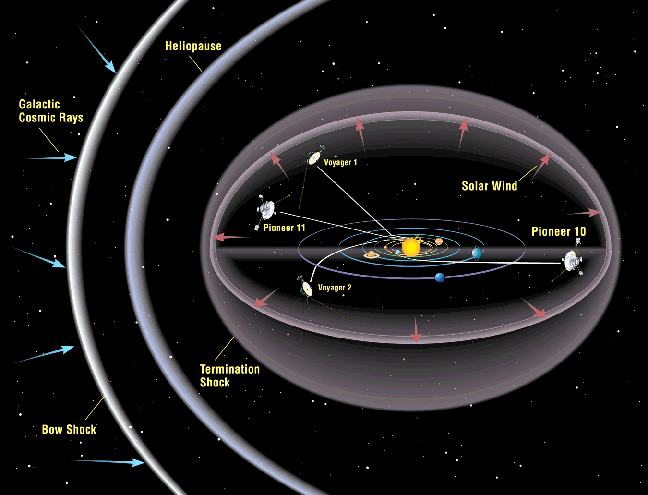
\includegraphics[max width=\linewidth]{../images/pioneer.png}\]

See how they'll eventually pass through a bubble called the
``termination shock''? That's where the solar wind drops below
supersonic speed as it crashes into the gas of the Milky Way. You can
see a pattern vaguely reminscient of the wave formed by a boat sailing
through the sea --- that's because we're moving through the Milky Way.

There are also two other spacecraft in this picture: Voyager 1 and 2!
These craft are still transmitting, and Voyager 1 is now farther than
Pioneer 10. It crossed the termination shock in December 2004, zipping
along at \(3.6\) AU per year. It's sending back information about this
region of space --- called the ``heliosheath'' --- and its batteries
should be good until 2020.

But what's the mystery?

Well, the Pioneer missions yielded the most precise information we have
about navigation in deep space. However, analysis of their radio
tracking data indicates a small unexplained acceleration towards the
Sun! The magnitude of this acceleration is roughly
10\textsuperscript{-9} meters per second per second. It's called the
``Pioneer anomaly''.

This anomaly has also been seen in the Ulysses spacecraft, and possibly
also in the Galileo spacecraft, though the data is much more noisy,
since these were Jupiter probes, hence much closer to the Sun, where
there is a lot more pressure from solar radiation. The Voyagers are not
set up to provide good data on this issue, since they are able to rotate
themselves and this messes things up. The Viking mission to Mars did
\emph{not} detect the Pioneer anomaly --- and it would have, had an
acceleration of this magnitude been present, because its radio tracking
was incredibly accurate --- good to about 12 meters.

Many physicists and astronomers have tried to explain the Pioneer
anomaly using conventional physics, but so far nobody seems to have
succeeded. Radiation pressure from the Sun, the solar wind, the
back-reaction from the radio emissions: all these point the wrong way!
Other explanations also seem to fail, like gravity from the Kuiper belt,
small amounts of gas venting from the spacecraft, and thermal radiation
from the craft,

As conventional explanations seemed to fail, people started trying to
explain the anomaly using new physics --- for example, modified theories
of gravity, or dark matter. But it's hard to get these explanations to
work, either. For example, explaining the Pioneer anomaly by the
gravitational attraction of dark matter would require more than .0003
solar masses of dark matter within 50 AU units of the Sun. But this is
in conflict with our highly successful calculations of planetary orbits
--- even a millionth of a solar mass of dark matter in this region would
be enough to throw those off!

So, we may have an interesting clue on our hands.

For more information on the Pioneer anomaly, see these sources and the
many references therein:

\begin{enumerate}
\def\labelenumi{\arabic{enumi})}
\setcounter{enumi}{5}
\item
  Wikipedia, ``Pioneer anomaly'',
  \texttt{http://en.wikipedia.org/wiki/Pioneer\_anomaly}
\item
  Chris P. Duif, ``Pioneer anomaly --- literature and links'',
  \texttt{http://www.space-time.info/pioneer/pioanomlit.html}
\end{enumerate}

I got interested in the Pioneer anomaly when I read this recent proposal
for a mission to study it:

\begin{enumerate}
\def\labelenumi{\arabic{enumi})}
\setcounter{enumi}{7}
\tightlist
\item
  The Pioneer Collaboration, ``A mission to explore the Pioneer
  anomaly'', available as
  \href{http://arxiv.org/abs/gr-qc/0506139}{\texttt{gr-qc/0506139}}.
\end{enumerate}

Finally, here's a fun book on the Pioneer missions:

\begin{enumerate}
\def\labelenumi{\arabic{enumi})}
\setcounter{enumi}{8}
\tightlist
\item
  Mark Wolverton, \emph{The Depths of Space: The Story of the Pioneer
  Planetary Probes}, Joseph Henry Press, 2004. Available at
  \texttt{http://www.nap.edu/books/0309090504/html/}
\end{enumerate}

Next: silicon lasers. I don't want to say much about these, just that
Intel thinks they could be the next big thing. You've probably heard
about ``Moore's Law'', how the number of components in an integrated
circuit doubles every 2 years. Or more vaguely: how computers keeping
getting more powerful, really fast! And you've probably heard that this
exponential growth is in danger of running into a brick wall someday.
One of the problems is that copper wire carries too little data, too
slowly.

For a long time some people have touted ``photonics'' as the way around
this: transmitting information as pulses of light, rather than clumps of
electrons. One problem is that substances that emit such pulses tend to
be expensive, like gallium arsenide and indium phosphide. But now
they've figured out to make silicon function as a laser! Researchers at
Intel have created a silicon laser that emits a continuous beam of
light. They've also developed a modulator that chops the beam into 10
billion pulses per second --- a 10 gigahertz signal.

For details, try this:

\begin{enumerate}
\def\labelenumi{\arabic{enumi})}
\setcounter{enumi}{9}
\item
  Intel, ``Silicon photonics'',
  \texttt{http://www.intel.com/technology/silicon/sp/}
\item
  Robert Service, ``Intel's breakthrough'', \emph{Technology Review},
  July 2005, 62--65. Also available at
  \texttt{http://www.technologyreview.com/articles/05/07/issue/feature\_intel.asp}
\end{enumerate}

While we're talking about high tech, how about quantum computers? Most
of them don't work very well --- yet, say the optimists. Interaction
with the environment ruins the coherence of the quantum state. But
there's a company called D-Wave Systems that aims to build a different
breed of quantum computer --- one that doesn't mind a fair amount of
noise. It's an analog chip made of lots of superconductors, which is
supposed to quantum tunnel to a lowest-energy state, The idea is that
you can get it to solve lots of minimization problems this way, like the
travelling salesman problem.

I don't see why it'll work better than other analogue computers, or
methods like simulated annealing. It could get stuck when there are lots
of ``almost-minima'' to sift through\ldots{} just like glass gets stuck
when it tries to find \emph{its} lowest energy state. Physicists call
this ``frustration'': the poor glass in your window is ``frustrated'',
trying to crystallize but unable to decide how to do it. In principle it
could do it by quantum tunnelling, but in practice that takes forever.
Why will D-Wave Systems' computer be better?

By the way, they admit their computer \emph{can't} do cool stuff like
rapidly factor large numbers via Shor's algorithm, the way full-fledged
quantum computers should. True devotees of quantum computation probably
wouldn't even call it a quantum computer! But I'll be happy if it works.

They've certain managed to convince some investors. Here's some more
info:

\begin{enumerate}
\def\labelenumi{\arabic{enumi})}
\setcounter{enumi}{11}
\tightlist
\item
  Erika Jonietz, ``Quantum calculation'', \emph{Technology Review}, July
  2005, 24--25. Also available at
  \texttt{http://www.technologyreview.com/articles/05/07/issue/forward\_quantum.asp}
\end{enumerate}

But enough practical stuff! Now let me say a bit more about the Klein
quartic.

I wrote about this gadget in \protect\hyperlink{week214}{``Week 214''}
and \protect\hyperlink{week215}{``Week 215''}. Simply put, this is a
``Platonic surface'': a \(3\)-holed torus tiled by regular heptagons,
with 3 heptagons meeting at each vertex.

It's perfectly symmetrical, but you can't stuff it into
\(3\)-dimensional Euclidean space without warping it. So, its charms are
a bit more esoteric than those of, say, a dodecahedron.

Of course, this is the kind of challenge that some people just can't
resist. Mike Stay and Gerard Westendorp bravely tried making paper
models of it:

\begin{enumerate}
\def\labelenumi{\arabic{enumi})}
\setcounter{enumi}{12}
\item
  Mike Stay, ``Klein quartic'',
  \texttt{http://math.ucr.edu/\textasciitilde{}mike/klein/}
\item
  Gerard Westendorp, ``Geometry'',
  \texttt{http://www.xs4all.nl/\textasciitilde{}westy31/Geometry/Geometry.html}
\end{enumerate}

Mike wisely stopped just short of the final step, which would create a
nasty crumpled mess. Gerard succeeded in completing the task by
switching to \emph{pastry} instead of paper. Check it out!

There might be a small niche market for Klein quartic birthday
cakes\ldots{} but computer graphics are probably better if you just want
to visualize this surface instead of actually eat it. About 10 or 12
years ago, Joe Christy made the following pictures using a program
called Geomview, which makes virtual 3d objects:

\begin{enumerate}
\def\labelenumi{\arabic{enumi})}
\setcounter{enumi}{14}
\tightlist
\item
  Joe Christy, Klein quartic pictures:\\
  \texttt{http://math.ucr.edu/home/baez/pentacontihexahedron.jpg}~\\
  \texttt{http://math.ucr.edu/home/baez/pentacontihexahedron2.jpg}~\\
  \texttt{http://math.ucr.edu/home/baez/pentacontihexahedron3.jpg}
\end{enumerate}

\[
  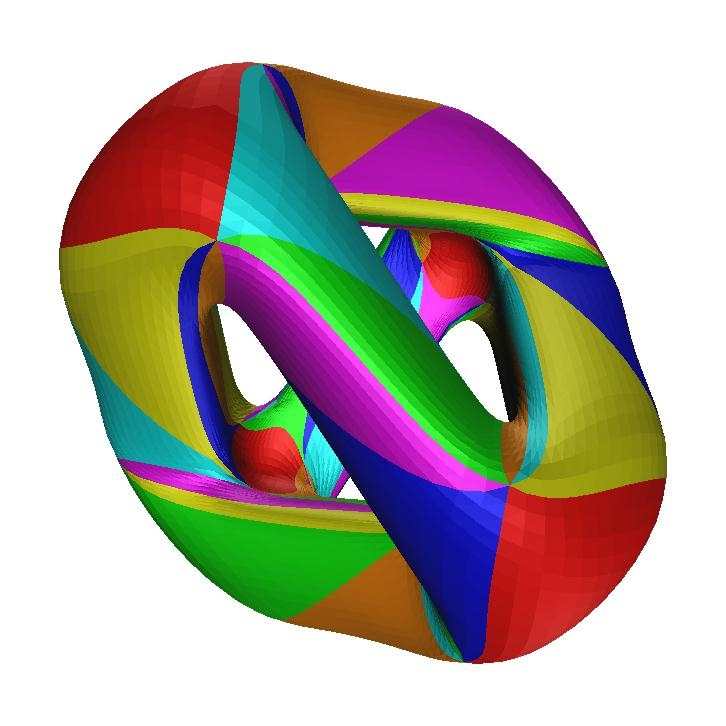
\includegraphics[max width=0.3\linewidth]{../images/pentacontihexahedron.jpg}
  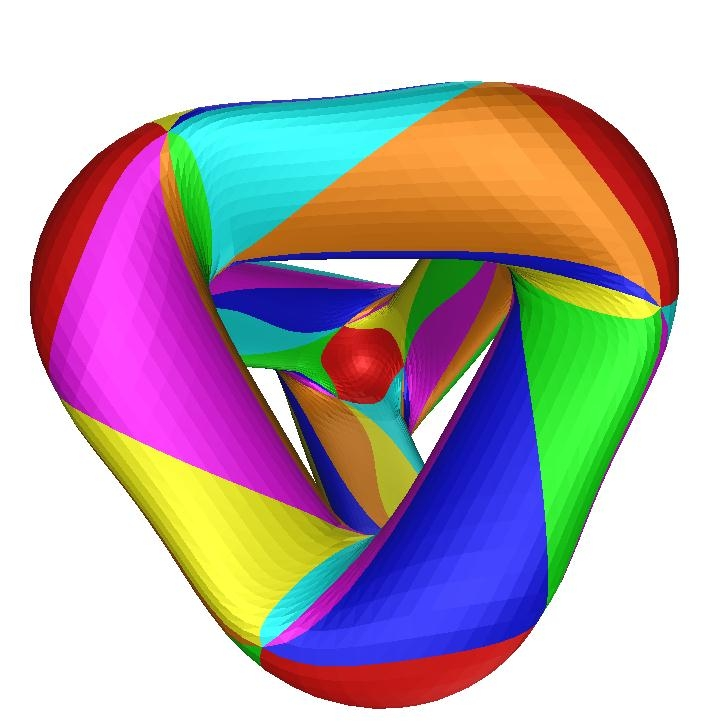
\includegraphics[max width=0.3\linewidth]{../images/pentacontihexahedron2.jpg}
  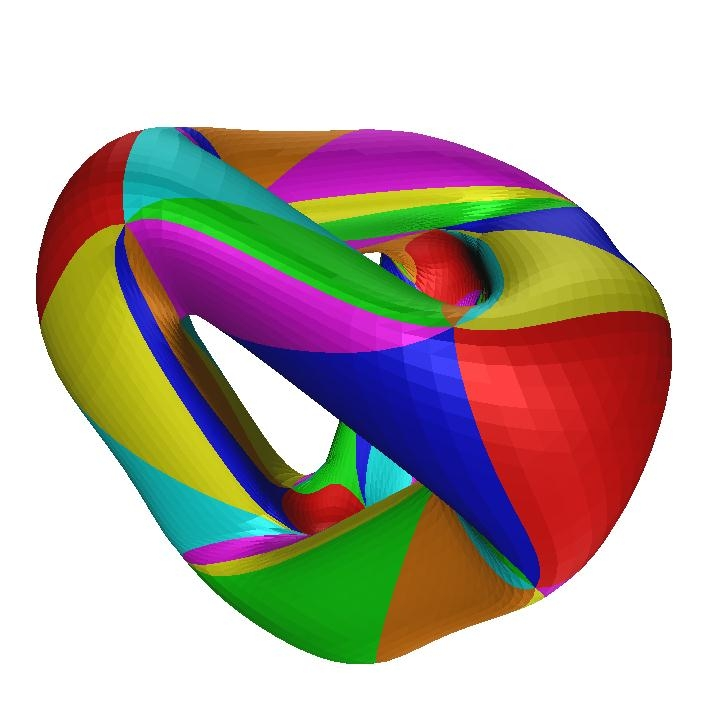
\includegraphics[max width=0.3\linewidth]{../images/pentacontihexahedron3.jpg}
\]

It took about a day on the fastest Linux machine they had at the time.
The advantage of Geomview is that once the virtual object is done, you
can quickly create different views. These pictures show the dual version
of Klein's quartic, which has 7 regular triangles meeting at each
quarter. The funky name ``pentacontihexahedron'' refers to the fact that
there are 56 of these triangles.

While I'm at it, I can't resist showing you another beautiful picture:

\begin{enumerate}
\def\labelenumi{\arabic{enumi})}
\setcounter{enumi}{15}
\tightlist
\item
  Joe Christy, ``Fano plane on Roman surface'',
  \texttt{http://math.ucr.edu/home/baez/roman.jpg}
\end{enumerate}

\[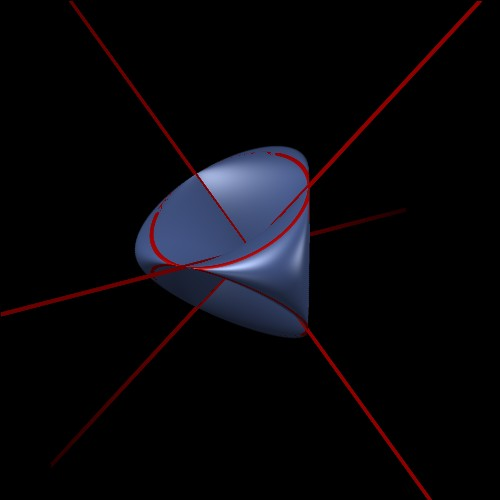
\includegraphics[max width=\linewidth]{../images/roman.jpg}\]

The blue thing is called the ``Roman surface'' because it was discovered
by the mathematician Jakob Steiner while he was visiting Rome. It's a
self-intersecting immersion of the projective plane in 3d space. On it,
the 7 lines of the Fano plane are visible in red, with four of them
drawn as circles.

Mathematically, one nice thing about this picture is that it exhibits
the tetrahedral symmetry of the Fano plane!

You can see all these pictures and much more on my Klein quartic
website:

\begin{enumerate}
\def\labelenumi{\arabic{enumi})}
\setcounter{enumi}{16}
\tightlist
\item
  John Baez, ``Klein's quartic curve'',
  \texttt{http://math.ucr.edu/home/baez/klein.html}
\end{enumerate}

You may think I'm digressing, but the relation between Klein's quartic
curve and the Fano plane underlies what I want to talk about today. Greg
Egan and I realized that this relation is just part of a bigger picture
involving special relativity in \(3\)-dimensional spacetime\ldots{} over
the integers \(\mod 7\).

Huh?

Well, these days so-called physicists have no shame studying physics in
all sorts of dimensions, but they usually confine themselves to building
their spacetimes out of the real numbers.

That makes sense if they're trying to claim some relevance to real-world
physics, however slight. But mathematically, there's no reason not to
try other number systems, like finite fields, just for the fun of it.

And this sheds new light on the Klein quartic. Why? Because the
symmetries of the Klein quartic and the Fano plane also act as
\emph{Lorentz transformations} in 3 dimensional spacetime if you work
using the integers \(\mod 7\). This lets us see the Klein quartic and
Fano plane as being closely related to special relativity in this funny
context.

Let's see how this goes.

First, recall that a ``field'' is a number system where you can add,
subtract, multiply and divide to your hearts content, with all the basic
laws holding that hold for real numbers. A ``finite field'' is one with
finitely many elements, like the integers mod any prime number \(p\).
This example is called \(\mathbb{Z}/p\), or \(\mathbb{F}_p\) if you
really want to emphasize that you're thinking of it as a field.

So, let's do some 3d special relativity with \(\mathbb{Z}/7\), and see
what it has to say about the Klein quartic.

First, some basic stuff about finite fields.

The concepts of ``positive'' and ``negative'' make sense in any finite
field! Say a nonzero element of the field is ``positive'' if it's of the
form \(x^2\) and ``negative'' otherwise. (Number theorists call the
positive elements ``quadratic residues'', just to intimidate outsiders.)

Then multiplication works nicely:

\begin{itemize}
\tightlist
\item
  if you multiply two positive elements you get a positive one;
\item
  if you multiply two negative elements you get a positive one;
\item
  if you multiply a positive and a negative element you get a negative
  one.
\end{itemize}

There are finite fields whose cardinality is any prime power, but if we
focus on those whose cardinality is a prime, namely the fields
\(\mathbb{Z}/p\), there are three possibilities: the good, the bad, and
the ugly.

\begin{itemize}
\tightlist
\item
  GOOD: If the field is \(\mathbb{Z}/p\) for \(p = 4n+3\) then \(-1\) is
  negative,\\
  so we can switch the ``sign'' of a number by multiplying it by \(-1\).
\item
  BAD: If the field is \(\mathbb{Z}/p\) for \(p = 4n+1\) then \(-1\) is
  positive,\\
  so we can't do this.
\end{itemize}

In both these cases there are as many positive as negative elements.
Then there's

\begin{itemize}
\tightlist
\item
  UGLY: If the field is \(\mathbb{Z}/2\) then every element is positive.
\end{itemize}

Luckily, \(p = 7\) is good. But beware: addition doesn't get along with
positivity very well. In fields like \(\mathbb{Z}/p\), \emph{every}
element is a sum of positive elements.

Next, let's ponder the peculiarities of special relativity over a finite
field.

We can define Minkowski spacetime of any dimension over any field
\(\mathbb{F}\): it's just \(\mathbb{F}^{n+1}\) with the quadratic form
\[x^2 = x_0^2 - x_1^2 - \ldots - x_n^2\] We define \(\mathrm{O}(n,1)\)
to be the group of transformations of \(\mathbb{F}^{n+1}\) that preserve
the above quadratic form, and define the ``Lorentz group''
\(\mathrm{SO}(n,1)\) to be the subgroup consisting of transformations
that also have determinant \(1\).

As usual, we say that a vector \(x\) in Minkowski spacetime is:

\begin{itemize}
\tightlist
\item
  timelike if \(x^2 > 0\)
\item
  lightlike if \(x^2 = 0\)
\item
  spacelike if \(x^2 < 0\)
\end{itemize}

We define a ``ray'' to be a line through the origin. We say a ray is
timelike, spacelike or lightlike if any vector on it --- hence all! ---
is of that type.

The lightlike rays are usually called ``light rays'', both because it
sounds cool (we went into physics because we liked things like X-rays
and rayguns) and because it's accurate. The light rays going through a
given point --- the origin --- are precisely like this.

Next, let's ponder the peculiarities of \(3\)-dimensional spacetime.

For any field \(\mathbb{F}\), \(2\times2\) matrices with determinant
\(1\) act as Lorentz transformations of 3d Minkowski spacetime. I
touched upon this idea when discussing Trautman's ``Pythagorean
spinors'' in \protect\hyperlink{week196}{``Week 196''}. Here's how it
works:

We can think of 3d Minkowski spacetime as consisting of all \(2\times2\)
matrices that are equal to their own transpose: \[
  x = \left(
    \begin{array}{cc}
      x_0+x_1 & x_2
    \\x_2 & x_0-x_1
    \end{array}
  \right)
\] since the determinant of such a matrix is just
\[x^2 = x_0^2 - x_1^2 - x_2^2\]

In this picture, the group \(\mathrm{SL}(2,\mathbb{F})\) consisting of
\(2\times2\) matrices with determinant \(1\) acts as Lorentz
transformations: \[g\colon x \mapsto gxg^*\] where \(g^*\) is the
transpose of \(g\). So, we get a homomorphism from
\(\mathrm{SL}(2,\mathbb{F})\) to the 3d Lorentz group:
\[\mathrm{SL}(2,\mathbb{F}) \to \mathrm{SO}(2,1)\] This is two-to-one,
since it sends both \(1\) and \(-1\) to the identity Lorentz
transformation. People typically cure this by defining
\[\mathrm{PSL}(2,\mathbb{F}) = \mathrm{SL}(2,\mathbb{F})/\{\pm1\}\] We
then get a one-to-one homomorphism
\[\mathrm{PSL}(2,\mathbb{F}) \to \mathrm{SO}(2,1)\] Alas, this
homomorphism is not onto: it's only ``half-onto''. In the traditional
case where \(\mathbb{F}\) is the real numbers, its range is just one of
the two connected components of \(\mathrm{SO}(2,1)\). In the case we're
interested in here, where \(\mathbb{F} = \mathbb{Z}/7\), the group
\(\mathrm{PSL}(2,\mathbb{Z}/7)\) has 168 elements but
\(\mathrm{SO}(2,1)\) has twice as many.

Next, let's bring the hyperbolic plane into the game!

Special relativity in 3 dimensions is closely related to the hyperbolic
plane. The reason is that the set of timelike rays in
\((n+1)\)-dimensional Minkowski spacetime forms a copy of hyperbolic
\(n\)-space: physicists call this the ``mass hyperboloid''. So, for
\(n = 2\), we get the hyperbolic plane. This is most familiar for
special relativity based on the real numbers, but the same idea applies
to other fields.

So, let's make some definitions:

\begin{itemize}
\tightlist
\item
  the hyperbolic plane \(H_+\) is the set of timelike rays in 3d
  Minkowski spacetime
\item
  the heavenly circle \(L\) is the set of light rays in 3d Minkowski
  spacetime
\item
  the hyperbolic cylinder \(H_-\) is the set of spacelike rays in 3d
  Minkowski spacetime
\end{itemize}

You may think I'm being silly to call the set of light rays ``the
heavenly circle'', but in \(4\)-dimensional spacetime the analogous
thing is often called ``the heavenly sphere'', and we're studying things
one dimension down.

Why ``heavenly sphere''? Well, when you look at the stars at night, they
seem to be lying on a sphere. That's the heavenly sphere: the set of
light rays entering your eye --- the set of directions you can look!

One dimension down, flatlanders get to enjoy the ``heavenly circle''.
Mathematicians call this the projective line, since it's a line with one
extra point added on.

Now for something fun: points on the hyperbolic plane give lines on the
hyperbolic cylinder and vice versa!

This is basically by definition of ``line''. We define a ``line'' in
\(H_+\) to consist of all points that are orthogonal to a given point in
\(H_-\), and vice versa. Note a point in either of these spaces is
really a ray in Minkowski spacetime, but it makes sense to say that two
rays are orthogonal.

This definition isn't arbitrary: it reduces to a standard notion of
``line'' in the hyperbolic plane --- namely a geodesic --- when our
field is the real numbers.

Finally, let's dive into the case we're really interested in:
\(3\)-dimensional Minkowski spacetime over
\(\mathbb{F} = \mathbb{Z}/7\).

In this case the positive numbers are \(1,2,4\), and the negative
numbers are \(3,5,6\).

It turns out that:

\begin{itemize}
\tightlist
\item
  The hyperbolic plane over \(\mathbb{Z}/7\), namely \(H_+\), has size
  21.
\item
  The heavenly circle over \(\mathbb{Z}/7\), namely \(L\), has size 8.
\item
  The hyperbolic cylinder over \(\mathbb{Z}/7\), namely \(H_-\), has
  size 28.
\end{itemize}

So, \(H_+\) is a nice finite version of the hyperbolic plane with 21
points and 28 lines! A little calculation shows there are 3 points on
each line and 4 lines through each point.

We know that \(\mathrm{PSL}(2,\mathbb{Z}/7)\) acts on everything in
sight here: \(H_+\), \(H_-\), and \(L\). It also acts on the Fano plane
and Klein's quartic curve. So, we can try to match up various features
of 3d special relativity with features in the Fano plane or Klein's
quartic curve!

Greg Egan found the following correspondence:

\begin{longtable}[]{@{}ll@{}}
\toprule
Hyperbolic plane over \(\mathbb{Z}/7\) & Fano plane\tabularnewline
\midrule
\endhead
7 triads & 7 points\tabularnewline
7 antitriads & 7 lines\tabularnewline
21 points & 21 flags\tabularnewline
28 lines & 28 apartments\tabularnewline
\bottomrule
\end{longtable}

As usual with these correspondences, simple things in the Fano plane
correspond to subtle things in the hyperbolic plane, and simple things
in the hyperbolic plane correspond to subtle things in the Fano plane.

First of all, points and lines in the Fano plane correspond to
``triads'' and ``antitriads'' in \(H_+\).

Huh?

Well, for starters, a ``triad'' or ``antitriad'' is an unordered triple
of orthogonal points in \(H_+\).

Huh?

Well, remember that a point in \(H_+\) is a timelike ray in 3d Minkowski
spacetime. You can't have three timelike rays that are orthogonal in
ordinary special relativity, but you can over \(\mathbb{Z}/7\), because
the sum of postive numbers can be zero, or even negative. For example,
these three vectors are timelike and orthogonal:
\[(1,0,0), \quad (0,4,2), \quad (0,-2,4)\] We call the corresponding
triple of rays a ``triad'', and we get a total of 7 triads by applying
elements of \(\mathrm{PSL}(2,\mathbb{Z}/7)\) to it. But, there are
triples of orthogonal timelike rays that aren't among these 7. For
example, we get one from these three vectors:
\[(1,0,0), \quad (0,2,4), \quad (0,-4,2)\] We call the corresponding
triple of rays an ``antitriad'', and we get 7 antitriads by applying
elements of \(\mathrm{PSL}(2,\mathbb{Z}/7)\).

Each line in the Fano plane contains 3 points, and each point lies on 3
lines. This incidence relation can also be seen in terms of triads and
antitriads: each triad has nonempty intersection with 3 antitriads, and
each antitriad has nonempty intersection with 3 triads!

We can also go backwards: points and lines in the hyperbolic plane
correspond to ``flags'' and ``apartments'' in the Fano plane.

Huh?

Flags and apartments are standard concepts in the theory of
``buildings'' which I began to explain in
\protect\hyperlink{week186}{``Week 186''}. But, I don't want or need to
explain this general theory here. In the Fano plane, a ``flag'' consists
of a point lying on a line: \[
  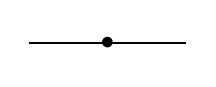
\begin{tikzpicture}
    \draw[thick] (0,0) to node{$\bullet$} (2,0);
  \end{tikzpicture}
\] An ``apartment'' consists of 3 distinct points lying on 3 distinct
lines like this: \[
  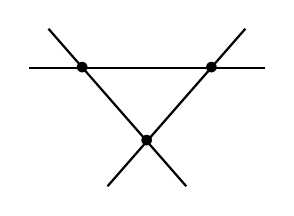
\begin{tikzpicture}
    \draw[thick] (0,0.5) to (3,0.5);
    \draw[thick] (0.25,1) to (2,-1);
    \draw[thick] (1,-1) to (2.75,1);
    \node at (0.68,0.5) {$\bullet$};
    \node at (2.32,0.5) {$\bullet$};
    \node at (1.5,-0.43) {$\bullet$};
  \end{tikzpicture}
\] Each apartment in the Fano plane contains 3 flags, and each flag is
contained in 4 apartments. This incidence can also been seen in terms of
points and lines in the hyperbolic plane: each line contains 3 points,
and each point lies on 4 lines!

So, there's an interesting but complicated relation between hyperbolic
geometry over \(\mathbb{Z}/7\) and the Fano plane. How does the Klein
quartic curve fit in? There's more to this side of the story than I've
managed to absorb, so I'll just say a few words --- probably more than
you want to hear. For more detail, try my Klein quartic curve webpage.

There are 48 nonzero lightlike vectors in 3d Minkowksi spacetime, but if
you take one of them and apply elements of
\(\mathrm{PSL}(2,\mathbb{Z}/7)\) to it, you get an orbit consisting of
only 24. These 24 guys correspond to the 24 heptagons in the heptagonal
tiling of the Klein quartic curve! In other words,
\(\mathrm{PSL}(2,\mathbb{Z}/7)\) acts in precisely the same way.

You may ask what the point of all this stuff is, and the answer is ---
I'm not sure yet, except that it's fun! Apparently the coincidence
\[\mathrm{PSL}(2,\mathbb{Z}/7) = \mathrm{PSL}(3,\mathbb{Z}/2)\] is the
only coincidence among classical groups over finite fields, not counting
the ones we already know over the real numbers. So, it's got to be good
for something! And, I haven't even begun to exploit the fact that the
Klein quartic curve is a quotient space of the real hyperbolic plane:
this has got to be related to the hyperbolic plane over
\(\mathbb{Z}/7\). So, I think something interesting should emerge,
though I'm not sure what.

\begin{center}\rule{0.5\linewidth}{0.5pt}\end{center}

\textbf{Addendum:} Regarding the Pioneer anomaly, the cosmologist Ned
Wright writes:

\begin{quote}
John,

I don't think the obvious possibilities have been ruled out. In this I
disagree with Anderson but that's science at the fringes.

I have a Web page on this at:\\
\texttt{http://www.astro.ucla.edu/\textasciitilde{}wright/PioneerAA.html}
\end{quote}

Just for the record, that's:

\begin{enumerate}
\def\labelenumi{\arabic{enumi})}
\setcounter{enumi}{16}
\tightlist
\item
  Ned Wright, ``Pioneer anomalous acceleration'',
  \texttt{http://www.astro.ucla.edu/\textasciitilde{}wright/PioneerAA.html}
\end{enumerate}

For a contrasting viewpoint see:

\begin{enumerate}
\def\labelenumi{\arabic{enumi})}
\setcounter{enumi}{17}
\tightlist
\item
  Slava G. Turyshev, Michael Martin Nieto, and John D. Anderson, ``The
  Pioneer anomaly and its implications'', available as
  \href{http://arxiv.org/abs/gr-qc/0510081}{\texttt{gr-qc/0510081}}.
\end{enumerate}

\begin{center}\rule{0.5\linewidth}{0.5pt}\end{center}

\begin{quote}
\emph{Space isn't remote at all. It's only an hour's drive away if your
car could go straight upwards.}

--- Sir Fred Hoyle
\end{quote}



\hypertarget{week220}{%
\section{August 31, 2005}\label{week220}}

Work on quantum gravity has seemed stagnant and stuck for the last
couple of years, which is why I've been turning more towards pure math.

Over in string theory they're contemplating a vast ``landscape'' of
possible universes, each with their own laws of physics --- one or more
of which might be ours. Each one is supposed to correspond to a
different ``vacuum'' or ``background'' for the marvelous unifying
M-theory that we don't completely understand yet. They can't choose the
right vacuum except by the good old method of fitting the experimental
data. But these days, this time-honored method gets a lot less airplay
than the ``anthropic principle'':

\begin{enumerate}
\def\labelenumi{\arabic{enumi})}
\tightlist
\item
  Leonard Susskind, ``The anthropic landscape of string theory'',
  available as
  \href{https://arxiv.org/abs/hep-th/0302219}{\texttt{hep-th/0302219}}.
\end{enumerate}

Perhaps this is because it's more grandiose to imagine choosing one
theory out of a multitude by discovering that it's among the few that
supports intelligent life, than by noticing that it correctly predicts
experimental results. Or, perhaps it's because nobody really knows how
to get string theory to predict experimental results! Even after you
chose a vacuum, you'd need to see how supersymmetry gets broken, and
this remain quite obscure.

There's still tons of beautiful math coming out of string theory, mind
you: right now I'm just talking about physics.

What about loop quantum gravity? This line of research has always been
less ambitious than string theory. Instead of finding the correct theory
of everything, its goal has merely been to find \emph{any} theory that
combines gravity and quantum mechanics in a background-free way. But, it
has major problems of its own: nobody knows how it can successfully
mimic general relativity at large length scales, as it must to be
realistic! Old-fashioned perturbative quantum gravity failed on this
score because it wasn't renormalizable. Loop quantum gravity may get
around this somehow\ldots{} but it's about time to see exactly how.

Loop quantum gravity follows two main approaches: the so-called
``Hamiltonian'' or ``spin network'' approach, which focuses on the
geometry of space at a given time, and the so-called ``Lagrangian'' or
``spin foam'' approach, which focuses on the geometry of spacetime.

In the last couple of years, the most interesting new work in the
Hamiltonian approach has focussed on problems with extra symmetry, like
black holes and the big bang. Here's a nontechnical introduction:

\begin{enumerate}
\def\labelenumi{\arabic{enumi})}
\setcounter{enumi}{1}
\tightlist
\item
  Abhay Ashtekar, ``Gravity and the quantum'', available as
  \href{https://arxiv.org/abs/gr-qc/0410054}{\texttt{gr-qc/0410054}}.
\end{enumerate}

and here's some new work that treats the information loss puzzle:

\begin{enumerate}
\def\labelenumi{\arabic{enumi})}
\setcounter{enumi}{2}
\tightlist
\item
  Abhay Ashtekar and Martin Bojowald, ``Black hole evaporation: a
  paradigm'', \emph{Class. Quant. Grav.} \textbf{22} (2005) 3349--3362.
  Also available as
  \href{https://arxiv.org/abs/gr-qc/0504029}{\texttt{gr-qc/0504029}}.
\end{enumerate}

However, by focusing on solutions with extra symmetry, one puts off
facing the hardest aspects of renormalization, or whatever its
equivalent might be in loop quantum gravity.

The other approach --- the spin foam approach --- got stalled when the
most popular model seemed to give spacetimes made mostly of
squashed-flat ``degenerate \(4\)-simplexes''. Various papers have found
an effect like this: see \protect\hyperlink{week198}{``Week 198''} for
more details. So, there's definitely a real phenomenon going on here.
However, its physical significance remains a bit obscure. The devil is
in the details.

In particular, even though the \emph{amplitude} for a single large
\(4\)-simplex in the Barrett-Crane model is dominated by degenerate
geometries, certain \emph{second derivatives} of the amplitude might not
--- and this may be what really matters. Carlo Rovelli has recently come
out with a paper on this:

\begin{enumerate}
\def\labelenumi{\arabic{enumi})}
\setcounter{enumi}{3}
\tightlist
\item
  Carlo Rovelli, ``Graviton propagator from background-independent
  quantum gravity'', available as
  \href{https://arxiv.org/abs/gr-qc/0508124}{\texttt{gr-qc/0508124}}.
\end{enumerate}

If the idea holds up, I'll be pretty excited. If not, I'll be bummed.
But luckily, I've already gone through the withdrawal pains of switching
my focus away from quantum gravity. When you do theoretical physics,
sometimes you feel the high of discovering hidden truths about the
physical universe. Sometimes you feel the agony of suspecting that those
``hidden truths'' were probably just a bunch of baloney\ldots{} or,
realizing that you may never know. Ultimately nature has the last word.

Math is, at least for me, a less nerve-racking pursuit, since the truths
we find can be confirmed simply by discussing them: we don't need to
wait for experiment. Math is just as grand as physics, or more so. But
it's more wispy and ethereal, since it's about pure pattern in general
--- not the particular magic patterns that became the world we see. So,
the stakes are lower, but the odds are higher.

Speaking of math, I really want to talk about the Streetfest --- the
conference in honor of Ross Street's 60th birthday. It was a real blast:
over sixty talks in two weeks in two cities, Sydney and Canberra.
However, I accidentally left my notes from those talks at home before
zipping off to Calgary for a summer school on homotopy theory:

\begin{enumerate}
\def\labelenumi{\arabic{enumi})}
\setcounter{enumi}{4}
\tightlist
\item
  \emph{Topics in Homotopy Theory}, graduate summer school at the
  Pacific Institute of Mathematics run by Kristine Bauer and Laura
  Scull. Recommended reading material available at
  \texttt{http://www.pims.math.ca/science/2005/05homotopy/reading.html}
\end{enumerate}

So, I'll say a bit about what I learned at this school.

Dan Dugger spoke about motivic homotopy theory, which was \emph{great},
because I've been trying to understand stuff from number theory and
algebraic geometry like the Weil conjectures, etale cohomology, motives,
and Voevodsky's proof of the Milnor conjecture\ldots{} and thanks to his
wonderfully pedagogical lectures, it's all starting to make some sense!

I hope to talk about this someday, but not now.

Alejandro Adem spoke about orbifolds and group cohomology. Purely
personally, the most exciting thing here was seeing that orbifolds can
also be seen as certain kinds of topological groupoids, or stacks, or
topoi\ldots{} so that various versions of ``categorified topology'' are
actually different faces of the same thing!

I may talk about this someday, too, but not now.

I spoke about higher gauge theory and its relation to Eilenberg-Mac Lane
spaces. I may talk about that too someday, but not now.

Dev Sinha spoke about operads, and besides explaining the basics, he
said a couple of things that really blew me away. So, I want to talk
about this now.

For one, the homology of the little \(k\)-cubes operad is a graded
version of the Poisson operad! For two, the little \(2\)-cubes operad
acts on the space of thickened long knots!

But for this to thrill you like it thrills me, I'd better say a word
about operads --- and especially little \(k\)-cubes operads.

Operads, and especially the little \(k\)-cubes operads, were invented by
Peter May in the early 1970s to formalize the algebraic structures
lurking in ``infinite loop spaces''. In
\protect\hyperlink{week149}{``Week 149''} I explained what infinite loop
spaces are, and how they give generalized cohomology theories, but let's
not get bogged down in this motivation now, since operads are actually
quite simple.

In its simplest form, an operad is a gizmo that has for each
\(n = 0,1,2,\ldots\) a set \(\mathcal{O}(n)\) whose elements are thought
of as \(n\)-ary operations --- operations with \(n\) inputs. It's good
to draw such operations as black boxes with \(n\) input wires and one
output: \[
  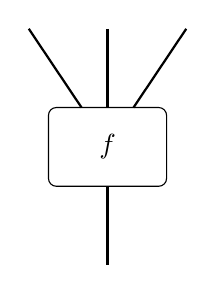
\begin{tikzpicture}
    \draw[thick] (-1,2) to (-0.33,1);
    \draw[thick] (0,2) to (0,1);
    \draw[thick] (1,2) to (0.33,1);
    \node at (0,0.5) {$f$};
    \draw[rounded corners=1mm] (-0.75,1) rectangle ++(1.5,-1);
    \draw[thick] (0,0) to (0,-1);
  \end{tikzpicture}
\] For starters these operations are purely abstract things that don't
actually operate on anything. Only when we consider a ``representation''
or ``action'' of an operad do they get incarnated as actual \(n\)-ary
operations on some set. The point of operads is to study their actions.

But, for completeness, let me sketch the definition of an operad. An
operad tells us how to compose its operations, like this: \[
  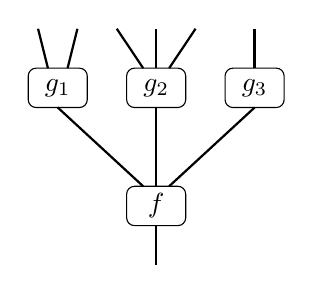
\begin{tikzpicture}[scale=0.5]
    \begin{scope}[shift={(-2.5,3)}]
      \draw[thick] (-0.5,2) to (-0.25,1);
      \draw[thick] (0.5,2) to (0.25,1);
      \node at (0,0.5) {$g_1$};
      \draw[rounded corners=1mm] (-0.75,1) rectangle ++(1.5,-1);
    \end{scope}
    \begin{scope}[shift={(0,3)}]
      \draw[thick] (-1,2) to (-0.33,1);
      \draw[thick] (0,2) to (0,1);
      \draw[thick] (1,2) to (0.33,1);
      \node at (0,0.5) {$g_2$};
      \draw[rounded corners=1mm] (-0.75,1) rectangle ++(1.5,-1);
    \end{scope}
    \begin{scope}[shift={(2.5,3)}]
      \draw[thick] (0,2) to (0,1);
      \node at (0,0.5) {$g_3$};
      \draw[rounded corners=1mm] (-0.75,1) rectangle ++(1.5,-1);
    \end{scope}
      \draw[thick] (-2.5,3) to (-0.33,1);
      \draw[thick] (0,3) to (0,1);
      \draw[thick] (2.5,3) to (0.33,1);
      \node at (0,0.5) {$f$};
      \draw[rounded corners=1mm] (-0.75,1) rectangle ++(1.5,-1);
      \draw[thick] (0,0) to (0,-1);
  \end{tikzpicture}
\] Here we are composing \(f\) with \(g_1\), \(g_2\), and \(g_3\) to get
an operation with 6 inputs called \(f\circ(g_1,g_2,g_3)\).

An operad needs to have a unary operation serving as the identity for
composition. It also needs to satisfy an ``associative law'' that makes
a composite of composites like this well-defined: \[
  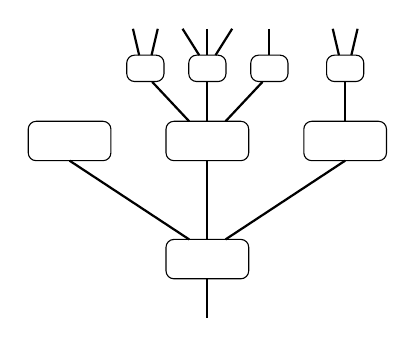
\begin{tikzpicture}[xscale=0.7,yscale=0.5]
    \begin{scope}[shift={(0,3)},xscale=0.45,yscale=0.67]
      \begin{scope}[shift={(-2.5,3)}]
        \draw[thick] (-0.5,2) to (-0.25,1);
        \draw[thick] (0.5,2) to (0.25,1);
        \draw[rounded corners=1mm] (-0.75,1) rectangle ++(1.5,-1);
      \end{scope}
      \begin{scope}[shift={(0,3)}]
        \draw[thick] (-1,2) to (-0.33,1);
        \draw[thick] (0,2) to (0,1);
        \draw[thick] (1,2) to (0.33,1);
        \draw[rounded corners=1mm] (-0.75,1) rectangle ++(1.5,-1);
      \end{scope}
      \begin{scope}[shift={(2.5,3)}]
        \draw[thick] (0,2) to (0,1);
        \draw[rounded corners=1mm] (-0.75,1) rectangle ++(1.5,-1);
      \end{scope}
    \end{scope}
    \begin{scope}[shift={(2.5,3)},xscale=0.45,yscale=0.67]
      \begin{scope}[shift={(0,3)}]
        \draw[thick] (-0.5,2) to (-0.25,1);
        \draw[thick] (0.5,2) to (0.25,1);
        \draw[rounded corners=1mm] (-0.75,1) rectangle ++(1.5,-1);
      \end{scope}
    \end{scope}
    \begin{scope}[shift={(-2.5,3)}]
      \draw[rounded corners=1mm] (-0.75,1) rectangle ++(1.5,-1);
    \end{scope}
    \begin{scope}[shift={(0,3)}]
      \draw[thick] (-1,2) to (-0.33,1);
      \draw[thick] (0,2) to (0,1);
      \draw[thick] (1,2) to (0.33,1);
      \draw[rounded corners=1mm] (-0.75,1) rectangle ++(1.5,-1);
    \end{scope}
    \begin{scope}[shift={(2.5,3)}]
      \draw[thick] (0,2) to (0,1);
      \draw[rounded corners=1mm] (-0.75,1) rectangle ++(1.5,-1);
    \end{scope}
      \draw[thick] (-2.5,3) to (-0.33,1);
      \draw[thick] (0,3) to (0,1);
      \draw[thick] (2.5,3) to (0.33,1);
      \draw[rounded corners=1mm] (-0.75,1) rectangle ++(1.5,-1);
      \draw[thick] (0,0) to (0,-1);
  \end{tikzpicture}
\] (This picture has a \(0\)-ary operation in it, just to emphasize that
this is allowed.)

That's the complete definition of a ``planar operad''. In a full-fledged
operad we can do more: we can permute the inputs of any operation and
get a new operation: \[
  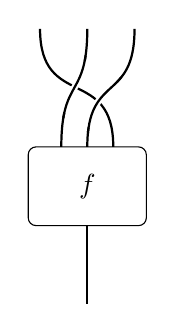
\begin{tikzpicture}
    \begin{knot}
      \strand[thick] (-0.6,2.5)
        to [out=down,in=up,looseness=1.5] (0.33,1);
      \strand[thick] (0,2.5)
        to [out=down,in=up,looseness=1.5] (-0.33,1);
      \strand[thick] (0.6,2.5)
        to [out=down,in=up,looseness=1.5] (0,1);
      \flipcrossings{1,2};
    \end{knot}
    \node at (0,0.5) {$f$};
    \draw[rounded corners=1mm] (-0.75,1) rectangle ++(1.5,-1);
    \draw[thick] (0,0) to (0,-1);
  \end{tikzpicture}
\] This gives actions of the permutation groups on the sets
\(\mathcal{O}(n)\). We also demand that these actions be compatible with
composition, in a way that's supposed to be obvious from the pictures.
For example: \[
  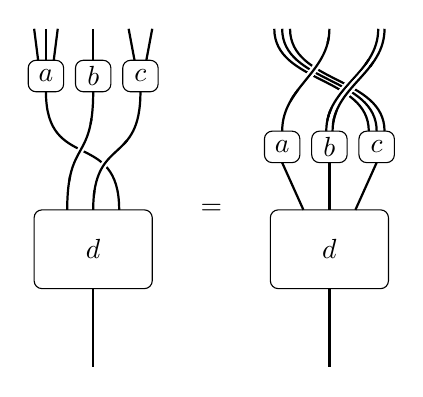
\begin{tikzpicture}
    \begin{knot}
      \strand[thick] (-0.6,2.5)
        to [out=down,in=up,looseness=1.5] (0.33,1);
      \strand[thick] (0,2.5)
        to [out=down,in=up,looseness=1.5] (-0.33,1);
      \strand[thick] (0.6,2.5)
        to [out=down,in=up,looseness=1.5] (0,1);
      \flipcrossings{1,2};
    \end{knot}
    \draw[rounded corners=1mm] (-0.75,1) rectangle ++(1.5,-1);
    \node at (0,0.5) {$d$};
    \draw[thick] (0,0) to (0,-1);
    \begin{scope}[xscale=0.3,yscale=0.4,shift={(-2,6.25)}]
      \draw[thick] (-0.5,2) to (-0.33,1);
      \draw[thick] (0,2) to (0,1);
      \draw[thick] (0.5,2) to (0.33,1);
      \draw[rounded corners=1mm] (-0.75,1) rectangle ++(1.5,-1);
      \node at (0,0.5) {$a$};
    \end{scope}
    \begin{scope}[xscale=0.3,yscale=0.4,shift={(0,6.25)}]
      \draw[thick] (0,2) to (0,1);
      \draw[rounded corners=1mm] (-0.75,1) rectangle ++(1.5,-1);
      \node at (0,0.5) {$b$};
    \end{scope}
    \begin{scope}[xscale=0.3,yscale=0.4,shift={(2,6.25)}]
      \draw[thick] (-0.5,2) to (-0.25,1);
      \draw[thick] (0.5,2) to (0.25,1);
      \draw[rounded corners=1mm] (-0.75,1) rectangle ++(1.5,-1);
      \node at (0,0.5) {$c$};
    \end{scope}
    \node at (1.5,1) {$=$};
    \begin{scope}[shift={(3,0)}]
      \draw[thick] (-0.6,1.6) to (-0.33,1);
      \draw[thick] (0,1.6) to (0,1);
      \draw[thick] (0.6,1.6) to (0.33,1);
      \draw[rounded corners=1mm] (-0.75,1) rectangle ++(1.5,-1);
      \node at (0,0.5) {$d$};
      \draw[thick] (0,0) to (0,-1);
      \begin{scope}[xscale=0.3,yscale=0.4,shift={(-2,4)}]
        \draw[rounded corners=1mm] (-0.75,1) rectangle ++(1.5,-1);
        \node at (0,0.5) {$a$};
      \end{scope}
      \begin{scope}[xscale=0.3,yscale=0.4,shift={(0,4)}]
        \draw[rounded corners=1mm] (-0.75,1) rectangle ++(1.5,-1);
        \node at (0,0.5) {$b$};
      \end{scope}
      \begin{scope}[xscale=0.3,yscale=0.4,shift={(2,4)}]
        \draw[rounded corners=1mm] (-0.75,1) rectangle ++(1.5,-1);
        \node at (0,0.5) {$c$};
      \end{scope}
      \begin{scope}[shift={(0,2)}]
        \begin{knot}
          \strand[thick] (0,1.3)
            to [out=down,in=up] (-0.6,0);
          \strand[thick] (0.62,1.3)
            to [out=down,in=up] (-0.04,0);
          \strand[thick] (0.7,1.3)
            to [out=down,in=up] (0.04,0);
          \strand[thick] (-0.7,1.3)
            to [out=down,in=up] (0.5,0);
          \strand[thick] (-0.6,1.3)
            to [out=down,in=up] (0.6,0);
          \strand[thick] (-0.5,1.3)
            to [out=down,in=up] (0.7,0);
        \end{knot}
      \end{scope}
    \end{scope}
  \end{tikzpicture}
\] and similarly for permuting the inputs of the black boxes on top.

\emph{Voilà!}

Now, operads make sense in various contexts. So far we've been talking
about operads that have a \emph{set} \(\mathcal{O}(n)\) of \(n\)-ary
operations for each n. These have actions on \emph{sets}, where each guy
in \(\mathcal{O}(n)\) gets incarnated as a \emph{function} that eats n
elements of some set and spits out an element of that set.

But historically, Peter May started by inventing operads that have a
\emph{topological space} of \(n\)-ary operations for each \(n\). These
like to act on \emph{topological spaces}, with the operations getting
incarnated as \emph{continuous maps}.

Most importantly, he invented an operad called the ``little \(k\)-cubes
operad''. Here \(\mathcal{O}(n)\) is the space of ways of putting \(n\)
nonoverlapping little \(k\)-dimensional cubes in a big one. We don't
demand that the little cubes are actually cubes: they can be rectangular
boxes. We do demand that their walls are nicely lined up with the walls
of the big cube: \[
  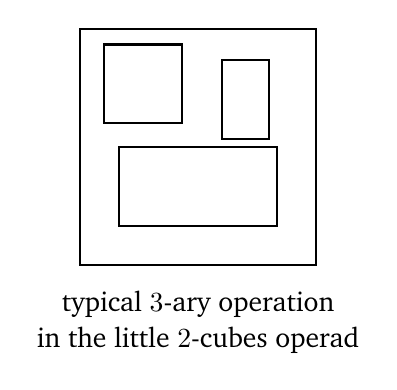
\begin{tikzpicture}
    \draw[thick] (0,0) rectangle ++(3,3);
    \draw[thick] (0.5,0.5) rectangle ++(2,1);
    \draw[thick] (0.3,1.8) rectangle ++(1,1);
    \draw[thick] (1.8,1.6) rectangle ++(0.6,1);
    \node at (1.5,-0.5) {typical $3$-ary operation};
    \node at (1.5,-0.95) {in the little $2$-cubes operad};
  \end{tikzpicture}
\] This is an operation in \(\mathrm{O}(3)\), where \(\mathcal{O}\) is
the little \(2\)-cubes operad. Or, at least it would be if I labelled
each of the 3 little \(2\)-cubes --- we need that extra information.

We compose operations by sticking pictures like this into each of the
little \(k\)-cubes in another picture like this! I should draw you an
example, but I'm too lazy. So, figure it out yourself and check the
associative law.

The reason this example is so important is that we get an action of the
little \(k\)-cubes operad whenever we have a ``\(k\)-fold loop space''.

Starting from a space \(S\) equipped with a chosen point \(*\), the
\(k\)-fold loop space \(\Omega^k(S)\) is the space of all maps from a
\(k\)-sphere into \(S\) that send the north pole to the point \(*\). But
this is also the space of all maps from a \(k\)-cube into \(S\) sending
the boundary of the \(k\)-cube to the point \(*\).

So, given \(n\) such such maps, we can glom them together using an
\(n\)-ary operation in the little \(k\)-cubes operad: \[
  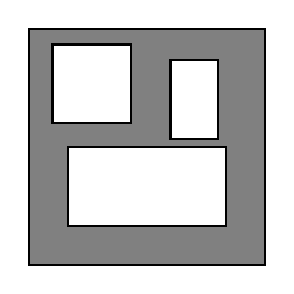
\begin{tikzpicture}
    \draw[thick,fill=gray] (0,0) rectangle ++(3,3);
    \draw[thick,fill=white] (0.5,0.5) rectangle ++(2,1);
    \draw[thick,fill=white] (0.3,1.8) rectangle ++(1,1);
    \draw[thick,fill=white] (1.8,1.6) rectangle ++(0.6,1);
  \end{tikzpicture}
\] where we map all the shaded stuff to the point \(*\). We get another
map from the \(k\)-cube to \(S\) sending the boundary to \(*\). So:

\begin{quote}
ANY \(k\)-FOLD LOOP SPACE HAS AN ACTION OF\\
THE LITTLE \(k\)-CUBES OPERAD
\end{quote}

But the really cool part is the converse:

\begin{quote}
ANY CONNECTED POINTED SPACE WITH AN ACTION OF\\
THE LITTLE \(k\)-CUBES OPERAD IS\\
HOMOTOPY EQUIVALENT TO A \(k\)-FOLD LOOP SPACE
\end{quote}

This is too technical to make a good bumper sticker, so if you want
people in your neighborhood to get interested in operads, I suggest
combining both the above slogans into one:

\begin{quote}
A \(k\)-FOLD LOOP SPACE IS THE SAME AS\\
AN ACTION OF THE LITTLE \(k\)-CUBES OPERAD
\end{quote}

Like any good slogan, this leaves out some important fine print, but it
gets the basic idea across. Modulo some details, being a \(k\)-fold loop
space amounts to having a bunch of operations: one for each way of
stuffing little \(k\)-cubes in a big one!

By the way:

Speaking of bumper stickers, I'm in Montreal now, and there's a funky
hangout on the Boulevard Saint-Laurent called Cafe \(\pi\) where people
play chess --- and they sell T-shirts, key rings, baseball caps and
coffee mugs decorated with the Greek letter \(\pi\)! The T-shirts are
great if you're going for a kind of math-nerd/punk look; I got one to
wow the students in my undergraduate courses. I don't usually provide
links to commercial websites, but I made an exception for Acme Klein
Bottles, and I'll make an exception for Cafe \(\pi\):

\begin{enumerate}
\def\labelenumi{\arabic{enumi})}
\setcounter{enumi}{5}
\tightlist
\item
  \(Cafe \pi\), \texttt{http://www.cafepi.ca/}
\end{enumerate}

Unfortunately they don't sell bumper stickers.

But where were we? Ah yes --- the little \(k\)-cubes operad.

The little \(k\)-cubes operad sits in the little \((k+1)\)-cubes operad
in an obvious way. Indeed, it's a ``sub-operad''. So, we can take the
limit as \(k\) goes to \(\infty\) and form the ``little \(\infty\)-cubes
operad''. Any infinite loop space gets an action of this\ldots{} and
that's why Peter May invented operads!

You can read more about these ideas in May's book:

\begin{enumerate}
\def\labelenumi{\arabic{enumi})}
\setcounter{enumi}{6}
\tightlist
\item
  J. Peter May, \emph{The Geometry of Iterated Loop Spaces}, Lecture
  Notes in Mathematics \textbf{271}, Springer, Berlin, 1972.
\end{enumerate}

or for a more gentle treatment, try this expository article:

\begin{enumerate}
\def\labelenumi{\arabic{enumi})}
\setcounter{enumi}{7}
\tightlist
\item
  J. Peter May, ``Infinite loop space theory'', \emph{Bull. Amer. Math.
  Soc.} \textbf{83} (1977), 456--494.
\end{enumerate}

But Dev Sinha told us about some subsequent work by Fred Cohen, who
computed the homology and cohomology of the little \(k\)-cubes operad.

For this, we need to think about operads in the world of linear algebra.
Here we consider operads that have a \emph{vector space} of \(n\)-ary
operations for each n, which get incarnated as \emph{multilinear maps}
when they act on some \emph{vector space}. These are sometimes called
``linear operads''.

An example is the operad for Lie algebras. This one is called ``Lie''.
\(\mathrm{Lie}(n)\) is the vector space of \(n\)-ary operations that one
can do whenever one has a Lie algebra. In this example:

\begin{itemize}
\item
  \(\mathrm{Lie}(0)\) is zero-dimensional, since there are no nullary
  operations (constants) built into the definition of Lie algebra,
  except zero.
\item
  \(\mathrm{Lie}(1)\) is one-dimensional, since the only unary
  operations are multiples of the identity operation: \[a \to a\]
\item
  \(\mathrm{Lie}(2)\) is one-dimensional, since the only binary
  operations are multiples of the Lie bracket: \[(a,b) \to [a,b]\] You
  might think we need a second guy in \(\mathrm{Lie}(2)\), namely
  \[(a,b) \to [b,a]\] but the antisymmetry of the Lie bracket says this
  is linearly dependent on the first one: \[[b,a] = -[a,b]\]
\item
  \(\mathrm{Lie}(3)\) is two-dimensional, since the only ternary
  operations are linear combinations of these two:
  \[(a,b,c) \to [a,b],c]\] \[(a,b,c) \to [b,[a,c]\] You might think we
  need a third guy in \(\mathrm{Lie}(3)\), for example
  \[(a,b,c) \to [a,[b,c]\] but the Jacobi identity says this is linearly
  dependent on the first two: \[[a,[b,c] = [a,b],c] + [b,[a,c]\]
\end{itemize}

You may enjoy trying to show that the dimension of \(\mathrm{Lie}(n)\)
is \((n-1)!\), at least for \(n > 0\). There's an incredibly beautiful
conceptual proof, and probably lots of obnoxious brute-force proofs.

There's a lot more to say about the Lie operad, but right now I want to
talk about the Poisson operad. A ``Poisson algebra'' is a commutative
associative algebra that has a bracket operation \(\{a,b\}\) making it
into a Lie algebra, with the property that
\[\{a,bc\} = \{a,b\}c + b\{a,c\}\] So, bracketing with any element is
like taking a derivative: it satisfies the product rule.

For this reason, Poisson algebras arise naturally as algebras of
observables in classical mechanics --- the Poisson bracket of any
observable \(A\) with an observable \(H\) called the ``Hamiltonian''
tells you the time derivative of \(A\): \[\frac{dA}{dt} = \{H,A\}\] This
is the beginning of a nice big story.

But, what's got me excited now is how Poisson algebras show up in
topology!

To understand this, we need to note that there's a linear operad whose
algebras are Poisson algebras. That's not surprising. But, we can get a
very similar operad in a rather shocking way, as follows.

Take the little \(k\)-cubes operad. This has a space \(\mathcal{O}(n)\)
of \(n\)-ary operations for each \(n\). Now take the homology of these
spaces \(\mathcal{O}(n)\), using coefficients in your favorite field,
and get vector spaces \(H(\mathcal{O}(n))\). By functorial abstract
nonsense these form a linear operad. And this is the operad for Poisson
algebras!

Alas, we actually have to be a bit more careful. The homology of each
space \(\mathcal{O}(n)\) with coefficients in some field is really a
\emph{graded} vector space over that field. So, taking the homology of
the little \(k\)-cubes operad gives an operad in the category of graded
vector spaces. And, it's the operad whose algebras are graded Poisson
algebras with a bracket of degree \(k-1\).

What are those? Well, they're like Poisson algebras, but if \(a\) is an
element of degree \(|a|\) and \(b\) is an element of degree \(|b|\),
then:

\begin{itemize}
\tightlist
\item
  \(ab\) has degree \(|a| + |b|\) (we've got a graded algebra)
\item
  \(\{a,b\}\) has degree \(|a| + |b| + k - 1\) (with a bracket of degree
  \(k-1\))
\end{itemize}

and the usual axioms for a Poisson algebra hold, but sprinkled with
minus signs according to the usual yoga of graded vector spaces.

So: whenever we have a \(k\)-fold loop space, its homology is a graded
Poisson algebra with a bracket of degree \(k-1\).

To get an idea of this works, let me sketch how the product and the
bracket work. Suppose we have an space \(X\) with an action of the
little \(k\)-cubes operad:

\begin{itemize}
\tightlist
\item
  The product on homology corresponds to sticking two little cubes side
  by side. Given two points in \(X\), this gives another point in \(X\).
  More generally, given two homology classes \(a\) and \(b\) in \(X\),
  we get a homology class of degree \(|a| + |b|\) in \(X\).
\item
  The bracket comes from taking one little cube and moving it around to
  trace out a sphere surrounding the other little cube. Given two points
  in \(X\), this gives a \((k-1)\)-sphere in \(X\). More generally,
  given a homology class \(a\) in \(X\), and a homology class \(b\) in
  \(X\), we get a homology class \(\{a,b\}\) of degree
  \(|a| + |b| + k - 1\).
\end{itemize}

The equation \[\{a,bc\} = \{a,b\}c + b\{a,c\}\] then says ``moving \(a\)
around \(b\) and \(c\) is like moving a around \(b\) while \(c\) stands
by, plus moving \(a\) around \(c\) while \(b\) stands by''.

I guess this result can be found here:

\begin{enumerate}
\def\labelenumi{\arabic{enumi})}
\setcounter{enumi}{8}
\item
  Frederick Cohen, ``Homology of \(\Omega^{n+1}\Sigma^{n+1}X\) and
  \(C_{n+1}X\), \(n>0\)'', \emph{Bull. Amer. Math. Soc.} \textbf{79}
  (1973), 1236--1241.
\item
  Frederick Cohen, Tom Lada and J. Peter May, \emph{The homology of
  iterated loop spaces}, Lecture Notes in Mathematics \textbf{533},
  Springer, Berlin, 1976.
\end{enumerate}

But, I don't think these old papers talk about graded Poisson operads!
Dev Sinha has a paper where he takes these ideas and distills them all
into the combinatorics of graphs and trees:

\begin{enumerate}
\def\labelenumi{\arabic{enumi})}
\setcounter{enumi}{10}
\tightlist
\item
  Dev Sinha, ``A pairing between graphs and trees'', available as
  \href{http://arxiv.org/abs/math.QA/0502547}{\texttt{math.QA/0502547}}.
\end{enumerate}

However, what I really like is how he gets these graphs and trees
starting from the homology and cohomology (respectively) of the little
\(k\)-cubes operad! He first wrote about it here:

\begin{enumerate}
\def\labelenumi{\arabic{enumi})}
\setcounter{enumi}{11}
\item
  Dev Sinha, ``Manifold theoretic compactifications of configuration
  spaces'', available as
  \href{http://arxiv.org/abs/math.GT/0306385}{\texttt{math.GT/0306385}}.

  Dev Sinha, ``The homology of the little disks operad'', available as
  \href{http://arxiv.org/abs/math/0610236}{\texttt{math/0610236}}.
\end{enumerate}

I have a vague feeling that this relation between the little \(k\)-cubes
operad and the Poisson operad is part of a big picture involving braids
and quantization. Another hint in this direction is Deligne's
Conjecture, now proved in many ways, which says that the operad of
singular chains coming from the little \(2\)-disks operad acts on the
Hochschild cochain complex of any associative algebra. Since Hochschild
cohomology classifies the ways you can deform an associative algebra,
this result is related to quantization and Poisson algebras. But, I
don't get the big picture! This might help:

\begin{enumerate}
\def\labelenumi{\arabic{enumi})}
\setcounter{enumi}{12}
\tightlist
\item
  Maxim Kontsevich, ``Operads and motives in deformation quantization'',
  \emph{Lett. Math. Phys.} \textbf{48} (1999) 35--72. Also available as
  \href{http://arxiv.org/math.QA/9904055}{\texttt{math.QA/9904055}}.
\end{enumerate}

I'd like to ponder this now! But I'm getting tired, and I still need to
say how the little \(2\)-cubes operad acts on the space of thickened
long knots.

What's a thickened long knot? In \(k\) dimensions, it's an embedding of
a little \(k\)-cube in a big one: \[f\colon [0,1]^k \to [0,1]^k\]
subject to the condition that the top and bottom of the little cube get
mapped to the top and bottom of the big one via the identity map. So,
you should imagine a thickened long knot as a fat square rope going from
the ceiling to the floor, all tied up in knots.

There are two ways to ``compose'' thickened long knots.

If you're a knot theorist, the obvious way is to stick one on top of the
other --- just like the usual composition of tangles. But if you just
think of thickened long knots as functions, you can also compose them
just by composing functions! This amounts to stuffing one knot inside
another\ldots{} a little hard to visualize, but fun.

Anyway, it turns out that the whole little \(2\)-cubes operad acts on
the space of thickened long knots, with the two operations \(I\) just
mentioned corresponding to this: \[
  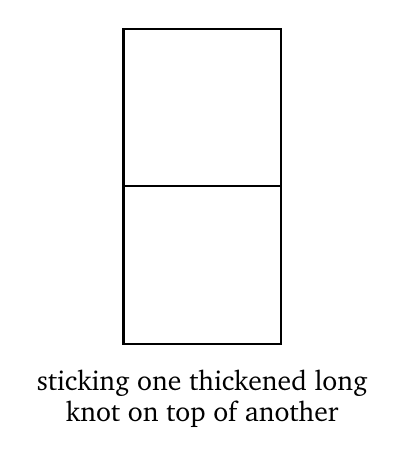
\begin{tikzpicture}
    \draw[thick] (0,0) rectangle (2,4);
    \draw[thick] (0,2) to (2,2);
    \node at (1,-0.5) {sticking one thickened long};
    \node at (1,-0.9) {knot on top of another};
  \end{tikzpicture}
\] and this: \[
  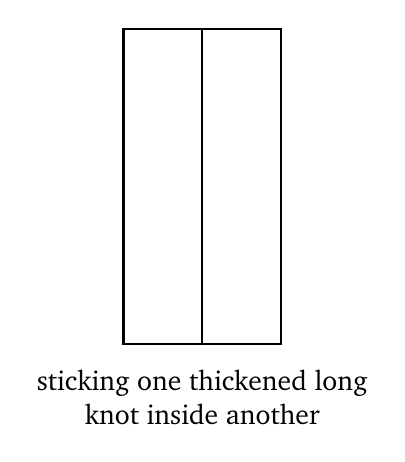
\begin{tikzpicture}
    \draw[thick] (0,0) rectangle (2,4);
    \draw[thick] (1,0) to (1,4);
    \node at (1,-0.5) {sticking one thickened long};
    \node at (1,-0.9) {knot inside another};
  \end{tikzpicture}
\] This isn't supposed to make obvious sense, but the point is, there
are lots of binary operations interpolating between these two --- one
for each binary operation in the little \(2\)-cubes operad!

This gives a new proof that the operation of ``sticking one thickened
long knot on top of another'' is commutative up to homotopy.

And, using these ideas, Ryan Budney has managed to figure out a lot of
information about the homotopy type of the space of long knots. Check
out these papers:

\begin{enumerate}
\def\labelenumi{\arabic{enumi})}
\setcounter{enumi}{13}
\item
  Ryan Budney, ``Little cubes and long knots'', available as
  \href{http://arxiv.org/math.GT/0309427}{\texttt{math.GT/0309427}}.
\item
  Ryan Budney and Frederick Cohen, ``On the homology of the space of
  long knots'', available as
  \href{http://arxiv.org/math.GT/0504206}{\texttt{math.GT/0504206}}.
\item
  Ryan Budney, ``Topology of spaces of knots in dimension 3'', available
  as \href{http://arxiv.org/math.GT/0506524}{\texttt{math.GT/0506524}}.
\end{enumerate}

The paper by Budney and Cohen combines the two ideas I just described
--- the action of the little \(2\)-cubes operad on thickened long knots
and its relation to the Poisson operad. Using these, they show that the
rational homology of the space of thickened long knots in 3 dimensions
is a free Poisson algebra! They also show that the mod-\(p\) homology of
this space is a free ``restricted Poisson'' algebra.

\begin{center}\rule{0.5\linewidth}{0.5pt}\end{center}

\textbf{Addendum:} Jesse McKeown had a question about the two operations
on long thickened knots. Here's what he asked:

\begin{quote}
Perhaps I'm being too imaginative, but I don't feel very convinced the
two operations described towards the end of
\protect\hyperlink{week220}{``Week 220''} are fundamentally different.

VagueSpecifically, in map-composition, can't one stretch all the
knottednes of the first composand into an ``upper'', essentially
unknotty portion of the second composand, and similarly squish the
knottedness of the second composand into a ``lower'' section of the big
all-encompassing box?
\end{quote}

Here's my reply:

\begin{quote}
Right! That's exactly what having an action of the little \(2\)-cubes
operad says! There's nothing ``fundamentally different'' between this:
\[
  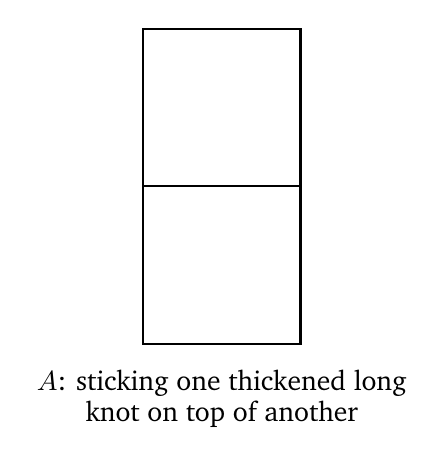
\begin{tikzpicture}
    \draw[thick] (0,0) rectangle (2,4);
    \draw[thick] (0,2) to (2,2);
    \node at (1,-0.5) {$A$: sticking one thickened long};
    \node at (1,-0.9) {knot on top of another};
  \end{tikzpicture}
\] and this: \[
  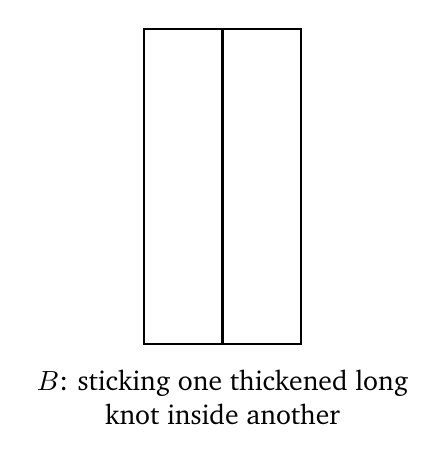
\begin{tikzpicture}
    \draw[thick] (0,0) rectangle (2,4);
    \draw[thick] (1,0) to (1,4);
    \node at (1,-0.5) {$B$: sticking one thickened long};
    \node at (1,-0.9) {knot inside another};
  \end{tikzpicture}
\] because there is a continuous family of operations interpolating
between these --- one for each way of sticking two little squares in a
big one.

But, the \emph{process} of moving from operation \(A\) to operation
\(B\) is itself nontrivial. If you loop all the way around from \(A\) to
\(B\) to \(A\) --- moving the two little squares around each other in
the big one --- you can get a noncontractible loop in the space of long
thickened knots!

And, this is what gives the bracket operation on the homology of the
space of thickened long knots.

Operads were born to deal with issues like this.
\end{quote}

On another note --- in the summer of 2007, Urs Schreiber posted a 3-part
article on Batalin--Vilkovisky quantization over at the \(n\)-Category
Cafe. The third part has links to the other two:

\begin{enumerate}
\def\labelenumi{\arabic{enumi})}
\setcounter{enumi}{17}
\tightlist
\item
  Urs Schreiber, ``Lyakhovich and Sharapov on QFT (On BV-Quantization,
  Part III)'',
  \texttt{http://golem.ph.utexas.edu/category/2007/08/lyakhonov\_and\_sharapov\_on\_qft.html}.
\end{enumerate}

and in addition to providing lots of references, it led me back to
puzzling about Poisson algebras and the little disks operad. Here's what
I wrote, roughly:

\begin{quote}
Try these:

\begin{enumerate}
\def\labelenumi{\arabic{enumi})}
\setcounter{enumi}{18}
\item
  Ezra Getzler, ``Batalin-Vilkovisky algebras and two-dimensional
  topological field theories'', \emph{Comm. Math. Phys.} \textbf{159}
  (1994), 265--285. Available at
  \texttt{http://projecteuclid.org/DPubS?service=UI\&version=1.0\&verb=Display\&handle=euclid.cmp/1104254599}
\item
  Takashi Kimura, Jim Stasheff and Alexander A. Voronov, ``On operad
  structures of moduli spaces and string theory'', \emph{Comm. Math.
  Phys.} \textbf{171} (1995), 1--25. ``Section 3.7: the
  Batalin-Vilkovisky (BV) algebra''. Available at
  \texttt{http://projecteuclid.org/DPubS?service=UI\&version=1.0\&verb=Display\&handle=euclid.cmp/1104273401}
\end{enumerate}

I don't understand this stuff very well!

More precisely:

If you take the space of multivector fields \(V\) on a manifold \(M\),
and think of \(V\) equipped with its wedge product and
\href{http://www.mimuw.edu.pl/~pwit/TOK/sem4/online/node9.html}{Schouten
bracket}, you get the easiest example of a
\href{http://golem.ph.utexas.edu/category/2007/02/infinitely_categorified_calcul.html}{Gerstenhaber
algebra}.

A Gerstenhaber algebra is an associative supercommutative graded algebra
\(A\) together with a bracket of degree \(-1\) which makes \(A\) into a
kind of ``graded Poisson algebra with bracket of degree \(-1\)''. All
the usual \href{http://en.wikipedia.org/wiki/Poisson_algebra}{Poisson
algebra} axioms hold, but sprinkled with minus signs according to the
usual conventions.

If your manifold \(M\) is a Poisson manifold, then the space \(V\) of
multivector fields comes equipped with a differential given by taking
the Schouten bracket with the Poisson bivector field \(\Pi\) in \(V\).

Axiomatizing this mess, we get the definition of a Batalin--Vilkovisky
algebra: a Gerstenhaber algebra with differential that's compatible with
the other structure in a certain way.

There are also lots of Batalin--Vilkovisky algebras that don't come from
Poisson manifolds. But just like Poisson manifolds, we can still think
of these as describing phase spaces in classical mechanics --- in a
clever algebraic way. And, that's what BV quantization is all about:
figuring out how to treat these Batalin-Vilkovisky algebras as classical
phase spaces and quantize them!

All this makes some sense to me. But then it gets weird and
mystical\ldots{}

First, thanks to an old result of Fred Cohen, a Gerstenhaber algebra is
the same as an algebra of the operad \(H(D)\) --- the homology of the
little disks operad!

Did I just hear some of you say ``Huh?''

Well, let me sketch what that means. The little disks operad is a gadget
with a bunch of \(n\)-ary operations corresponding to ways of sticking
\(n\) little disks in a big one. For each \(n\) there's a topological
space of these \(n\)-ary operations. Taking the homology of this
topological space, we get a graded vector space. These are the \(n\)-ary
operations of the operad I'm calling \(H(D)\).

While I roughly follow how this works, I don't understand the deep inner
meaning. It seems amazing: there's a mystical relation between ways of
sticking little 2d disks in bigger ones, and operations you can do on
the space of multivector fields on a manifold!

I don't know if the connections to 2d topological and conformal field
theory (described in the articles I cite) actually \emph{explain} this
mystical relation, or merely \emph{exploit} it.

Now, as I said, a Batalin--Vilovisky algebra is a Gerstenhaber algebra
with an extra operation. And, Getzler showed that this extra operation
corresponds to our ability to \emph{twist} a little disk \(360^\circ\).
(Until we started twisting like this, we could equally have used little
\(2\)-cubes.)

More precisely, Getzler showed that a Batalin--Vilkovisky algebra is the
same as an algebra of the homology of the \emph{framed} little discs
operad.

This extra twist of the knife only makes me more curious to know what's
\emph{really going on here}.

Here's a clue that could help. As I explained to Urs a couple days ago,
this business of ``taking homology'' is really some sort of procedure
for turning weak \(\infty\)-groupoids (i.e.~spaces) into stable strict
\(\infty\)-groupoids (i.e.~chain complexes) --- followed by taking the
homology of the chain complex, which in principle loses even \emph{more}
information, but doesn't in this particular example. That suggests that
these Gerstenhaber (and Batalin--Vilkovisky) algebras are really just
watered-down chain complex versions of \emph{spaces} equipped with
\(n\)-ary operations corresponding to ways of sticking \(n\) (framed)
little disks into a big disk.

But still: \emph{what's really going on? What do classical phase spaces
have to do with little \(2\)-dimensional disks???}

As far as I'm concerned, the Rosetta Stone on the third page of
Getzler's paper only serves to heighten the mystery further!
\end{quote}

\begin{center}\rule{0.5\linewidth}{0.5pt}\end{center}

\begin{quote}
\emph{One gets the impression that some physicists have gone for so long
without any experimental data that might resolve the quantum-gravity
debates that they are going a little crazy.}

---
\href{http://www.americanscientist.org/template/BookReviewTypeDetail/assetid/45919;jsessionid=baaayg8keWDBEI}{Jaron
Lanier}
\end{quote}



\hypertarget{week221}{%
\section{September 18, 2005}\label{week221}}

After going to the Streetfest this summer, I wandered around China. I
began by going to a big conference in Beijing, the 22nd International
Congress on the History of Science. I learned some interesting stuff.
For example:

You may have heard of
\href{http://en.wikipedia.org/wiki/Andalusia}{Andalusia,} that
fascinating melting-pot of cultures that formed when southern Spain was
invaded by Muslims. The eleventh century was the golden age of
Andalusian astronomy and mathematics, with a lot of innovation in
astrolabes. During the
\href{http://en.wikipedia.org/wiki/Timeline_of_the_Muslim_Occupation_of_the_Iberian_Peninsula}{Caliphate}
(929--1031), three quarters of all mathematical manuscripts were
produced in
\href{http://lexicorient.com/spain/photos/cordoba02.jpg}{Cordoba}, most
of the rest in
\href{http://images.encarta.msn.com/xrefmedia/sharemed/targets/images/pho/t054/T054900A.jpg}{Sevilla},
and only a few in
\href{http://lexicorient.com/spain/photos/granada02.jpg}{Granada} and
\href{http://hopf.chem.brandeis.edu/Milos/PhotoMD/Images/Spain2001/Toledo_Alcazar.JPG}{Toledo}.

I didn't understand the mathematical predominance of Cordoba when I
first heard about it, but the underlying reason is simple. The first
great Muslim dynasty were the
\href{http://en.wikipedia.org/wiki/Umayyads}{Ummayyads}, who ruled from
Damascus. They were massacred by the
\href{http://en.wikipedia.org/wiki/Abbasid}{Abbasids} in 750, who then
moved the capital to Baghdad. When
\href{http://en.wikipedia.org/wiki/Abd-ar-Rahman_I}{Abd ar-Rahman} fled
Damascus in 750 as the only Ummayyad survivor of this massacre, he went
to Spain, which had already been
\href{http://en.wikipedia.org/wiki/Muslim_conquest_of_Iberia}{invaded by
Muslim Berbers} in 711.

Abd ar-Rahman made Cordoba his capital. And, by enforcing a certain
level of religious tolerance, he made this city into \emph{the place to
be} for Muslims, Jews and Christians --- the ``ornament of the world'',
and a beacon of learning --- until it was sacked by Berber troops in
1009.

Other cities in Andalusia became important later. The great philosopher
\href{http://en.wikipedia.org/wiki/Averroes}{Ibn Rushd} --- known to
Westerners by the Latin name ``Averroes'' --- was born in Cordoba in
1128. He later became a judge there. He studied mathematics, medicine,
and astronomy, and wrote detailed line-by-line commentaries on the works
of Aristotle. It was through these commentaries that most of Aristotle's
works, including his Physics, found their way into Western Europe! By
1177, the bishop of Paris had banned the teaching of many of these new
ideas --- but to little effect.

Toledo seems to have only gained real prominence after
\href{http://en.wikipedia.org/wiki/Alfonso_VI_of_Castile}{Alfonso VI}
made it his capital upon capturing it in 1085 as part of the Christian
``reconquista''. By the 1200s, it became a lively center for translating
Arabic and Hebrew texts into Latin.

Mathematics also passed from the Arabs to Western Europe in other ways.
\href{http://www-groups.dcs.st-and.ac.uk/~history/Mathematicians/Fibonacci.html}{Fibonacci}
(1170-1250) studied Arabic accounting methods in North Africa where his
father was a diplomat. His book \emph{Liber Abaci} was important in
transmitting the Indian system of numerals (including zero) from the
Arabs to Europe. However, he wasn't the first to bring these numbers to
Europe. They'd been around for over 200 years!

For example:
\href{http://en.wikipedia.org/wiki/Gerbert_of_Aurillac}{Gerbert
d'Aurillac} (940--1003) spent years studying mathematics in various
Andalusian cities including Cordoba. On his return to France, he wrote a
book about a cumbersome sort of ``abacus'' labelled by a Western form of
the Indian numerals --- close to what we now call ``Arabic numerals''.
This remained popular in intellectual circles until the mid-12th
century.

Amusingly, Arabic numerals were also called ``dust numerals'' since they
were used in calculations on an easily erasable ``dust board''. Their
use was described in the \emph{Liber Pulveris}, or ``book of dust''.

I want to learn more about Andalusian science! I found this book a great
place to start --- it's really fascinating:

\begin{enumerate}
\def\labelenumi{\arabic{enumi})}
\tightlist
\item
  Maria Rose Menocal, \emph{The Ornament of the World: How Muslims, Jews
  and Christians Created a Culture of Tolerance in Medieval Spain},
  Little, Brown and Co., 2002.
\end{enumerate}

For something quick and pretty, try this:

\begin{enumerate}
\def\labelenumi{\arabic{enumi})}
\setcounter{enumi}{1}
\tightlist
\item
  Steve Edwards, ``Tilings from the Alhambra'',
  \texttt{http://www2.spsu.edu/math/tile/grammar/moor.htm}
\end{enumerate}

Apparently 13 of the 17 planar symmetry groups can be found in tile
patterns in the Alhambra, a Moorish palace built in Granada in the
1300s.

To dig deeper into the splendors of Arabic mathematics, try these:

\begin{enumerate}
\def\labelenumi{\arabic{enumi})}
\setcounter{enumi}{2}
\item
  John J. O'Connor and Edmund F. Robertson, ``Arabic mathematics:
  forgotten brilliance?'',
  \texttt{http://www-groups.dcs.st-and.ac.uk/\textasciitilde{}history/HistTopics/Arabic\_mathematics.html}

  John J. O'Connor and Edmund F. Robertson, ``Biographies of
  Arab/Islamic mathematicians'',
  \texttt{http://www-groups.dcs.st-and.ac.uk/\textasciitilde{}history/Indexes/Arabs.html}
\end{enumerate}

For more on Fibonacci and Arabic mathematics, try this paper by Charles
Burnett, who spoke about the history of ``Arabic numerals'' in Beijing:

\begin{enumerate}
\def\labelenumi{\arabic{enumi})}
\setcounter{enumi}{3}
\tightlist
\item
  Charles Burnett, ``Leonard of Pisa and Arabic Arithmetic'',
  \texttt{http://muslimheritage.com/topics/default.cfm?ArticleID=472}
\end{enumerate}

Another interesting talk in Beijing was about the role of the Syriac
language in the transmission of Greek science to Europe. Many important
texts didn't get translated directly from Greek to Arabic! Instead, they
were first translated into \emph{Syriac}.

I don't understand the details yet, but luckily there's a great book on
the subject, available free online:

\begin{enumerate}
\def\labelenumi{\arabic{enumi})}
\setcounter{enumi}{4}
\tightlist
\item
  De Lacy O'Leary, \emph{How Greek Science Passed to the Arabs},
  Routledge \& Kegan Paul Ltd, 1949. Also available at
  \texttt{http://www.aina.org/books/hgsptta.htm}
\end{enumerate}

So, medieval Europe learned a lot of Greek science by reading Latin
translations of Arab translations of Syriac translations of second-hand
copies of the original Greek texts!

George Baloglu recommends this book:

\begin{enumerate}
\def\labelenumi{\arabic{enumi})}
\setcounter{enumi}{5}
\tightlist
\item
  Dimitri Gutas, \emph{Greek Thought, Arabic Culture: The Graeco--Arabic
  Translation Movement in Baghdad and Early 'Abbasid Society
  (2nd--4th/8th--10th Centuries)}, Routledge, 1998.
\end{enumerate}

I want to read this book, too:

\begin{enumerate}
\def\labelenumi{\arabic{enumi})}
\setcounter{enumi}{6}
\tightlist
\item
  Scott L. Montgomery, \emph{Science in Translation: Movements of
  Knowledge through Cultures and Time}, U. of Chicago Press, 2000.
  Review by William R. Everdell available at MAA Online,
  \texttt{http://www.maa.org/publications/maa-reviews/science-in-translation-movements-of-knowledge-through-cultures-and-time}
\end{enumerate}

The historian of science John Stachel, famous for his studies of
Einstein, says this book ``strikes a blow at one of the founding myths
of `Western Civilization'\,'' --- namely, that Renaissance Europeans
single-handedly picked up doing science where the Greeks left off. As
Everdell writes in his review:

\begin{quote}
Perhaps the best of the book's many delightful challenges to
conventional wisdom comes in the first section on the translations of
Greek science. Here we learn why it is ridiculous to use a phrase like
``the Renaissance recovery of the Greek classics''; that in fact the
Renaissance recovered very little from the original Greek and that it
was long before the Renaissance that Aristotle and Ptolemy, to name the
two most important examples, were finally translated into Latin. What
the Renaissance did was to create a myth by eliminating all the
intermediate steps in the transmission. To assume that Greek was
translated into Arabic ``still essentially erases centuries of history''
(p.~93). What was translated into Arabic was usually Syriac, and the
translators were neither Arabs (as the great Muslim historian
\href{http://en.wikipedia.org/wiki/Ibn_Khaldun}{Ibn Khaldun} admitted)
nor Muslims. The real story involves Sanskrit compilers of ancient
Babylonian astronomy, Nestorian Christian Syriac-speaking scholars of
Greek in the Persian city of
\href{http://en.wikipedia.org/wiki/Jundishapur}{Jundishapur}, and
Arabic- and Pahlavi-speaking Muslim scholars of Syriac, including the
Nestorian Hunayn
\href{http://www.nestorian.org/hunein_ibn_ishak.html}{Ibn Ishak}
(809--873) of Baghdad, ``the greatest of all translators during this
era'' (p.~98).
\end{quote}

And now for something completely different: the Langlands program! I
want to keep going on my gradual quest to understand and explain this
profoundly difficult hunk of mathematics, which connects number theory
to representations of algebraic groups. I've found this introduction to
be really helpful:

\begin{enumerate}
\def\labelenumi{\arabic{enumi})}
\setcounter{enumi}{7}
\tightlist
\item
  Stephen Gelbart: ``An elementary introduction to the Langlands
  program'', \emph{Bulletin of the AMS} \textbf{10} (1984), 177--219.
\end{enumerate}

There are a lot of more detailed sources of information on the Langlands
program, but the problem for the beginner (me) is that the overall goal
gets swamped in a mass of technicalities. Gelbart's introduction does
the best at avoiding this problem.

I've also found parts of this article to be helpful:

\begin{enumerate}
\def\labelenumi{\arabic{enumi})}
\setcounter{enumi}{8}
\tightlist
\item
  Edward Frenkel, ``Recent advances in the Langlands program'',
  available at
  \href{http://arxiv.org/abs/math.AG/0303074}{\texttt{math.AG/0303074}}.
\end{enumerate}

It focuses on the ``geometric Langlands program'', which I'd rather not
talk about now. But, it starts with a pretty clear introduction to the
basic Langlands stuff\ldots{} at least, clear to me after I've battered
my head on this for about a year!

If you know some number theory or you followed recent issues This Week's
Finds (especially \protect\hyperlink{week217}{``Week 217''} and
\protect\hyperlink{week218}{``Week 218''}) it should make sense, so I'll
quote it:

\begin{quote}
The Langlands Program has emerged in the late 60's in the form of a
series of far-reaching conjectures tying together seemingly unrelated
objects in number theory, algebraic geometry, and the theory of
automorphic forms. To motivate it, recall the classical Kronecker-Weber
theorem which describes the maximal abelian extension
\(\mathbb{Q}^{\mathrm{ab}}\) of the field \(\mathbb{Q}\) of rational
numbers (i.e., the maximal extension of \(\mathbb{Q}\) whose Galois
group is abelian). This theorem states that \(\mathbb{Q}^{\mathrm{ab}}\)
is obtained by adjoining to \(\mathbb{Q}\) all roots of unity; in other
words, \(\mathbb{Q}^{\mathrm{ab}}\) is the union of all cyclotomic
fields \(\mathbb{Q}(1^{\frac1N})\) obtained by adjoining to
\(\mathbb{Q}\) a primitive \(N\)th root of unity \[1^{\frac1N}\] The
Galois group \(\mathrm{Gal}(Q(1^{\frac1N})/\mathbb{Q})\) of
automorphisms of \(\mathbb{Q}(1^{\frac1N})\) preserving \(\mathbb{Q}\)
is isomorphic to the group \((\mathbb{Z}/N)^*\) of units of the ring
\(\mathbb{Z}/N\). Indeed, each element \(m\) in \((\mathbb{Z}/N)^*\),
viewed as an integer relatively prime to \(N\), gives rise to an
automorphism of \(\mathbb{Q}(1^{\frac1N})\) which sends \[1^{\frac1N}\]
to \[1^{\frac{m}{N}}.\] Therefore we obtain that the Galois group
\(\mathrm{Gal}(\mathbb{Q}^{\mathrm{ab}}/\mathbb{Q})\), or, equivalently,
the maximal abelian quotient of
\(\mathrm{Gal}(\overline{\mathbb{Q}}/\mathbb{Q})\), where
\(\overline{\mathbb{Q}}\) is an algebraic closure of \(\mathbb{Q}\), is
isomorphic to the projective limit of the groups \((\mathbb{Z}/N)^*\)
with respect to the system of surjections
\[(\mathbb{Z}/N)^* \to (\mathbb{Z}/M)^*\] for \(M\) dividing \(N\). This
projective limit is nothing but the direct product of the multiplicative
groups of the rings of \(p\)-adic integers, \(\mathbb{Z}_p^*\), where
\(p\) runs over the set of all primes. Thus, we obtain that
\[\mathrm{Gal}(\mathbb{Q}^{\mathrm{ab}}/\mathbb{Q}) = \prod \mathbb{Z}_p^*.\]
The abelian class field theory gives a similar description for the
maximal abelian quotient
\(\mathrm{Gal}(\mathbb{F}^{\mathrm{ab}}/\mathbb{F})\) of the Galois
group \(\mathrm{Gal}(\overline{\mathbb{F}}/\mathbb{F})\), where
\(\mathbb{F}\) is an arbitrary global field, i.e., a finite extension of
\(\mathbb{Q}\) (number field), or the field of rational functions on a
smooth projective curve defined over a finite field (function field).
Namely, \(\mathrm{Gal}(\mathbb{F}^{\mathrm{ab}}/\mathbb{F})\) is almost
isomorphic to the quotient \(A(\mathbb{F})^*/\mathbb{F}^*\), where
\(A(\mathbb{F})\) is the ring of adeles of \(\mathbb{F}\), a subring in
the direct product of all completions of \(\mathbb{F}\). Here we use the
word ``almost'' because we need to take the group of components of this
quotient if \(\mathbb{F}\) is a number field, or its profinite
completion if \(\mathbb{F}\) is a function field.

When \(\mathbb{F} = \mathbb{Q}\) the ring \(A(\mathbb{Q})\) is a subring
of the direct product of the fields \(\mathbb{Q}_p\) of \(p\)-adic
numbers and the field \(\mathbb{R}\) of real numbers, and the quotient
\(A(\mathbb{F})^*/\mathbb{F}^*\) is isomorphic to
\[\mathbb{R}^+ \times \prod_p \mathbb{Z}_p^*.\] where \(\mathbb{R}^+\)
is the multiplicative group of positive real numbers. Hence the group of
its components is \[\prod_p \mathbb{Z}_p^*\] in agreement with the
Kronecker-Weber theorem.

One can obtain complete information about the maximal abelian quotient
of a group by considering its one-dimensional representations. The above
statement of the abelian class field theory may then be reformulated as
saying that one-dimensional representations of
\(\mathrm{Gal}(\overline{\mathbb{F}}/\mathbb{F})\) are essentially in
bijection with one-dimensional representations of the abelian group
\[A(\mathbb{F})^* = \mathrm{GL}(1,A(\mathbb{F}))\] which occur in the
space of functions on
\[A(\mathbb{F})^*/\mathbb{F}^* = \mathrm{GL}(1,A(\mathbb{F}))/\mathrm{GL}(1,\mathbb{F})\]
A marvelous insight of Robert Langlands was to conjecture that there
exists a similar description of \emph{\(n\)-dimensional representations}
of \(\mathrm{Gal}(\overline{\mathbb{F}}/\mathbb{F})\). Namely, he
proposed that those may be related to irreducible representations of the
group \(\mathrm{GL}(n,A(\mathbb{F}))\) which are \emph{automorphic},
that is those occurring in the space of functions on the quotient
\[\mathrm{GL}(n,A(\mathbb{F}))/\mathrm{GL}(n,\mathbb{F})\] This relation
is now called the \emph{Langlands correspondence}.

At this point one might ask a legitimate question: why is it important
to know what the \(n\)-dimensional representations of the Galois group
look like, and why is it useful to relate them to things like
automorphic representations? There are indeed many reasons for that.
First of all, it should be remarked that according to the Tannakian
philosophy, one can reconstruct a group from the category of its
finite-dimensional representations, equipped with the structure of the
tensor product. Therefore looking at \(n\)-dimensional representations
of the Galois group is a natural step towards understanding its
structure. But even more importantly, one finds many interesting
representations of Galois groups in ``nature''.

For example, the group
\(\mathrm{Gal}(\overline{\mathbb{Q}}/\mathbb{Q})\) will act on the
geometric invariants (such as the etale cohomologies) of an algebraic
variety defined over \(\mathbb{Q}\). Thus, if we take an elliptic curve
\(E\) over \(\mathbb{Q}\), then we will obtain a two-dimensional Galois
representation on its first etale cohomology. This representation
contains a lot of important information about the curve \(E\), such as
the number of points of \(E\) over \(\mathbb{Z}/p\) for various primes
\(p\).

The point is that the Langlands correspondence is supposed to relate
\(n\)-dimensional Galois representations to automorphic representations
of \(\mathrm{GL}(n,A(\mathbb{F}))\) in such a way that the data on the
Galois side, such as the number of points of \(E\) over
\(\mathbb{Z}/p\), are translated into something more tractable on the
automorphic side, such as the coefficients in the \(q\)-expansion of the
modular forms that encapsulate automorphic representations of
\(\mathrm{GL}(2,A(\mathbb{Q}))\).

More precisely, one asks that under the Langlands correspondence certain
natural invariants attached to the Galois representations and to the
automorphic representations be matched. These invariants are the
\emph{Frobenius conjugacy classes} on the Galois side and the
\emph{Hecke eigenvalues} on the automorphic side.
\end{quote}

Since I haven't talked about Hecke operators yet, I'll stop here!

But, someday I should really explain the ideas behind the baby
``abelian'' case of the Langlands philosophy in simpler terms than
Frenkel does here. The abelian case goes back way before Langlands: it's
called ``class field theory''. And, it's all about exploiting this
analogy, which I last mentioned in \protect\hyperlink{week218}{``Week
218''}:

\begin{longtable}[]{@{}ll@{}}
\toprule
Number theory & Complex geometry\tabularnewline
\midrule
\endhead
Integers & Polynomial functions on the complex plane\tabularnewline
Rational numbers & Rational functions on the complex
plane\tabularnewline
Prime numbers & Points in the complex plane\tabularnewline
Integers \(\mod p^n\) & \((n-1)\)st-order Taylor series\tabularnewline
\(p\)-adic integers & Taylor series\tabularnewline
\(p\)-adic numbers & Laurent series\tabularnewline
Adeles for the rationals & Adeles for the rational
functions\tabularnewline
Fields & One-point spaces\tabularnewline
Homomorphisms to fields & Maps from one-point spaces\tabularnewline
Algebraic number fields & Branched covering spaces of the complex
plane\tabularnewline
\bottomrule
\end{longtable}

\begin{center}\rule{0.5\linewidth}{0.5pt}\end{center}

\textbf{Addendum:} I thank Fabien Besnard for some suggestions on how to
improve this Week's Finds. Bruce Smith, Noam Elkies, and Miguel
Carrión-Álvarez had some things to say about the history of science. In
response to this comment of mine:

\begin{quote}
So, medieval Europe learned a lot of Greek science by reading Latin
translations of Arab translations of Syriac translations of second-hand
copies of the original Greek texts!
\end{quote}

my friend Bruce wrote:

\begin{quote}
This all seems so precarious a process that it makes me wonder whether
there was ten times as much valuable ancient math and philosophy as we
know about, most of which got \emph{completely} lost.
\end{quote}

Something like this almost certainly true.

Like Plato, Aristotle is believed to have written dialogs which
presented his ideas in a polished form. They were all lost. His extant
writings are just "lecture notesquot; for courses he taught!

Euripides wrote at least 75 plays, of which only 19 survive in their
full form. We have fragments or excerpts of some more. This isn't
philosophy or math, but it's still incredibly tragic (pardon the pun).

The mathematician Apollonius wrote a book on \emph{Tangencies} which is
lost. Only four of his eight books on \emph{Conics} survive in Greek.
Luckily, the first seven survive in Arabic.

The burning of the library of Alexandria is partially to blame for these
losses.

There's some good news, though:

Archimedes did more work on calculus than previously believed! We know
this now because a manuscript of his on mechanics that had been erased
and written over has recently been read with the help of a synchrotron
X-ray beam! This is a great example of modern science helping the
history of science.

This manuscript, called the Archimedes Palimpsest, also reveals for the
first time that he did work on combinatorics:

\begin{enumerate}
\def\labelenumi{\arabic{enumi})}
\setcounter{enumi}{9}
\item
  Nova, ``The Archimedes Palimpsest'',
  \texttt{http://www.pbs.org/wgbh/nova/archimedes/palimpsest.html}
\item
  Heather Rock Woods, ``Placed under X-ray gaze, Archimedes manuscript
  yields secrets lost to time'', \emph{Stanford Report}, May 19, 2005,
  \texttt{http://news-service.stanford.edu/news/2005/may25/archimedes-052505.html}
\item
  Erica Klarreich, ``Glimpses of genius: mathematicians and historians
  piece together a puzzle that Archimedes pondered'', \emph{Science
  News} \textbf{165} (2004), 314. Also available at
  \texttt{http://www.sciencenews.org/articles/20040515/bob9.asp}
\end{enumerate}

Also: a team using ``multispectral imaging'' has recently been able to
read parts of a Roman library in the town of
\href{http://en.wikipedia.org/wiki/Herculaneum}{Herculaneum}. The books
in this library were ``roasted in place'' --- heavily carbonized ---
during the eruption of Vesuvius that destroyed
\href{http://en.wikipedia.org/wiki/Pompeii}{Pompeii}. By distinguishing
between different shades of black, researchers were able to reconstruct
the entire book \emph{On Piety} by one Philodemus:

\begin{enumerate}
\def\labelenumi{\arabic{enumi})}
\setcounter{enumi}{12}
\tightlist
\item
  Julie Walker, ``A library of mud and ashes'', \emph{BYU Magazine},
  Spring 2001, \texttt{http://magazine.byu.edu/?act=view\&a=43}
\end{enumerate}

I can't resist quoting a bit:

\begin{quote}
A sister city to Pompeii that was also buried in the volcanic eruption
of A.D. 79, Herculaneum was a seaside town that sat between Vesuvius'
fertile foot and the gleaming Bay of Naples. The collection of 2,000
carbonized Greek and Latin scrolls, primarily Epicurean philosophical
writings, was found in a luxurious Herculaneum house known as the Villa
of the Papyri, which was discovered in 1752.

The scrolls have endured a destructive path through history: first, rain
soaked the papyri, then a 570-degree swell of molasses-thick mud
engulfed the villa and charred the scrolls. They would remain buried
under 65 feet of mud for hundreds of years.

As a result, many of the fragile scroll cylinders are pressed into
trapezoidal columns; some are bowed and snaked into half-moons, others
folded into v-shapes.

After their discovery the mortality rate for the scrolls continued to
climb as would-be conservators struggled to find a way to unroll the
fragile manuscripts. Some scrolls were turned to mush when they were
painted with mercury; many were sliced down the middle and cut into
fragments. Early transcribers would copy the visible outer layer of a
scroll, then scrape it off and discard it to read the next layer.

Even today, scholars use metaphors of near impossibility to describe the
scroll unrolling process. It is like ``flattening out a potato chip''
without destroying it, or like ``separating (burned) layers of two-ply
tissue,'' says Jeffrey Fish of Baylor University.

The current unrolling methoddeveloped by a team of Norwegian
conservators involves applying a gelatin-based adhesive to the scroll's
outer surface. As the adhesive dries, the outer shell --- which bears
the text on its interior --- can be slowly peeled off. It can take days
to remove a single fragment, months or years to process a complete
scroll. Some 300 of the library's scrolls have yet to be unrolled, and
many more scrolls are in various stages of conservation and repair.

On the Herculaneum project, CPART researchers Steve and Susan Booras
conducted multispectral imaging (MSI) on 3,100 trays of papyrus
fragments and photographed them with a high-quality digital camera. The
images will be used to create a digital library that can be accessed by
scholars worldwide. Developed for NASA scientists, the imaging technique
has only recently been applied to the study of ancient texts. Rather
than focusing on light that is seen at wave lengths visible to the eye,
MSI uses filters to focus on nonvisible portions of the light spectrum.
In the nonvisible infrared spectrum, the black ink on a blackened scroll
can be clearly differentiated. In some cases clear, legible writings
have been found on fragments that researchers believed were completely
blank.
\end{quote}

The same team is now studying over 400,000 fragments of papyrus found in
an ancient garbage dump in the old Egyptian town of
\href{http://en.wikipedia.org/wiki/Oxyrhynchus}{Oxyrhynchus}. They've
pieced together new fragments of plays by Euripides, Sophocles and
Menander, lost lines from the poets Sappho, Hesiod, and Archilocus, and
most of a book by Hesiod:

\begin{enumerate}
\def\labelenumi{\arabic{enumi})}
\setcounter{enumi}{13}
\tightlist
\item
  Oxyrhynchus Online, ``multispectral imaging'',
  \texttt{http://www.papyrology.ox.ac.uk/multi/procedure.html}
\end{enumerate}

If you just want to look at a nice ``before and after'' movie of what
multispectral imaging can do, try this link.

Finally, in response to this remark of mine:

\begin{quote}
Amusingly, Arabic numerals were also called ``dust numerals'' since they
were used in calculations on an easily erasable ``dust board''. Their
use was described in the Liber Pulveris, or ``book of dust''.
\end{quote}

Noam Elkies wrote:

\begin{quote}
This is even more amusing than you may realize: the word ``abacus''
comes from a Greek word ``abax, abak-'' for ``counting board'', which
conjecturally might come from the Hebrew word (or a cognate word in
another semitic language) for ``dust''! See for instance:

\texttt{http://education.yahoo.com/reference/dictionary/entry/abacus}

So these ``dust numerals'' replaced a reckoning device whose name may
also originate with calculation a dust board\ldots{}
\end{quote}

Interesting! While ``calculus'' refers back to pebbles.

My erstwhile student Miguel Carrión-Álvarez clarified the issue
somewhat:

\begin{quote}
The first abaci were drawn in the sand with sticks. The next step was to
carve grooves in a board (wooden, or clay: think cuneiform tablets) and
place beads in them. Pierced beads moving on beams (wood, later metal)
must have been a pretty recent development, relatively speaking.

Remember that Archimedes was studying geometry by drawing figures in the
sand when he was slain. If a sand abacus is the precursor of the modern
calculator, Archimedes' sandbox is the precursor of GUI geometry
software.

One of Archimedes' most fanciful works is ``The Sand Reckoner''. Here
the reckoner can be understood to be himself, as he is counting the
grains of sand which fit inside the sphere of fixed stars, but it can
also refer to a sand abacus (reckoner = calculator). In fact, romance
translations of this title that I've seen (French: L'arenaire, Spanish:
El arenario, etc.) unambiguously refer to an object, not a person. It is
easy to imagine Archimedes inventing his positional number system on a
sand abacus, and using the counting of grains of sand as an excuse to
write about it.
\end{quote}

\begin{center}\rule{0.5\linewidth}{0.5pt}\end{center}

\begin{quote}
\emph{We avail ourselves of what our predecessors may have said. That
they were or were not our coreligionists is of no account\ldots.
Whatever accords with the truth, we shall happily and gratefully accept,
and whatever conflicts, we shall scrupulously but generously point out.}

--- Averroes
\end{quote}



\hypertarget{week222}{%
\section{October 17, 2005}\label{week222}}

Last week there was a big conference on quantum gravity at the Albert
Einstein Institute near Berlin:

\begin{enumerate}
\def\labelenumi{\arabic{enumi})}
\tightlist
\item
  Loops '05, \texttt{http://loops05.aei.mpg.de}
\end{enumerate}

The focus was loop quantum gravity and spin foams, but there were also
talks about other approaches, so it was much bigger than last year's
get-together in Marseille. Last year about 100 people attended; this
time about 160 did! It was strange seeing old pals like Ashtekar,
Lewandowski, Loll, Rovelli and Smolin almost lost in a sea of new faces.
But, it was great to talk to everyone, both old and new.

I'll say more about this conference, but first let's talk about
\(\gamma\) ray bursters, a black hole without a host galaxy, the newly
discovered moon of planet Xena, and lots of other transneptunian
objects.

Actually, just for fun, let's start with this science fiction novel I
picked up in Heathrow en route to Berlin:

\begin{enumerate}
\def\labelenumi{\arabic{enumi})}
\setcounter{enumi}{1}
\tightlist
\item
  Charles Stross, \emph{Accelerando}, Ace Books, New York. Also
  available at \texttt{http://www.accelerando.org/book/}
\end{enumerate}

This is one of the few tales I've read that does a good job of fleshing
out Verner Vinge's ``Singularity'' scenario, where the accelerating
development of technology soars past human comprehension and undergoes a
phase transition to a thoroughly different world. This is a real
possibility, and it's been discussed a lot:

\begin{enumerate}
\def\labelenumi{\arabic{enumi})}
\setcounter{enumi}{2}
\item
  Wikipedia, ``Technological singularity'',
  \texttt{http://en.wikipedia.org/wiki/Technological\_singularity}

  Ray Kurzweil, ``The Singularity'',
  \texttt{http://www.kurzweilai.net/meme/frame.html?m=1}

  Anders Sandberg, ``The Singularity'',
  \texttt{http://www.aleph.se/Trans/Global/Singularity/}
\end{enumerate}

However, it's not an easy subject for fiction --- at least not for mere
human readers! Stross makes it gripping: sometimes goofy, sometimes
thrilling, and sometimes rather sad. Characters include a robot cat with
ever-growing powers and some space-faring uploaded lobsters.

The hero, Manfred Macx, starts out as a freeware developer, futurist and
all-purpose wheeler-dealer. Here's a scene from the beginning of the
book, before all hell breaks loose:

\begin{quote}
Manfred's mood of dynamic optimism is gone, broken by the knowledge that
his vivisectionist stalker has followed him to Amsterdam to say nothing
of Pamela, his dominatrix, source of so much yearning and so many
morning-after weals. He slips his glasses on, takes the universe off
hold, and tells it to take him for a long walk while he catches up on
the latest on the tensor-mode gravitational waves in the cosmic
background radiation (which, it is theorized, may be waste heat
generated by irreversible computational processes back during the
inflationary epoch; the present-day universe being merely the data left
behind by a really huge calculation). And then there's the weirdness
beyond M31: according to the more conservative cosmologists, an alien
superpower --- maybe a collective of Kardashev Type Three
galaxy-spanning civilizations --- is running a timing channel attack on
the computational ultrastructure of space-time itself, trying to break
through to whatever's underneath. The tofu-Alzheimer's link can wait.
\end{quote}

An idea a minute --- and the book is free online: what more could you
want?

But right now, the big news in astronomy is \emph{not} about a type III
civilization lurking beyond M31 (otherwise known as the Andromeda
Galaxy). It's some evidence that short \(\gamma\) ray bursts are caused
by collisions involving neutron stars and black holes!

\(\gamma\) ray bursts are among the most energetic events known in the
heavens. They happen in galaxies throughout the universe; we see about
one a day, and each releases somewhere between \(10^{45}\) and
\(10^{47}\) joules of energy. The larger figure is what you'd get by
turning the entire mass of the Sun into energy.

There could be several kinds of \(\gamma\) ray bursts, but there seem to
be at least two: short and long. Short bursts last between 40
milliseconds and 10 seconds --- imagine the whole Sun turning into
energy that fast! Long ones last between 10 and 100 seconds. The two
kinds seem to be qualitatively different: for example, the short ones
consist of higher-frequency \(\gamma\) rays. The big news is that they
happen in different kinds of galaxies!

In \protect\hyperlink{week204}{``Week 204''}, I described how people
caught a long \(\gamma\) ray burst in the act in March 2003. A
\(\gamma\) ray detector aboard a satellite relayed information to
telescopes in Australia and Japan, allowing them to spot a visible
afterglow right after the burst. The details of this glow fit the
``hypernova'' theory of long \(\gamma\) ray bursts.

The hypernova theory says that when a star more than 25 times heavier
than the Sun runs out of fuel and collapses, it forms a black hole that
sucks down the star's iron core before a normal supernova explosion can
occur. In just a few seconds, about a solar mass of iron spirals into
the black hole, forming a pancake-shaped disk as it goes down. In the
process, this disk becomes incredibly hot and shoots out jets of
radiation in the transverse directions. As they plow through the star's
outer layers, these jets create beams of \(\gamma\) rays.

The short bursts have been harder to catch. By the time a telescope on
Earth could be aimed at the spot where the \(\gamma\) rays were seen, no
afterglow could be seen!

So, in October 2004 NASA launched Swift: a \(\gamma\)-ray detecting
satellite equipped with an X-ray telescope and an ultraviolet/optical
telescope that can respond quickly whenever a burst is seen:

\begin{enumerate}
\def\labelenumi{\arabic{enumi})}
\setcounter{enumi}{3}
\item
  Official NASA Swift homepage,
  \texttt{http://swift.gsfc.nasa.gov/docs/swift/swiftsc.html}
\item
  Gamma-ray burst real-time sky map, \texttt{http://grb.sonoma.edu/}
\end{enumerate}

On May 9th, 2005, Swift detected a short burst and caught 11 photons of
the burst's X-ray afterglow. Another short burst detected by HETE-II had
its X-ray afterglow caught by the Chandra X-ray satellite. Analysis of
these and two more short bursts has convinced some scientists that
they're caused by collisions between neutron stars and/or black holes:

\begin{enumerate}
\def\labelenumi{\arabic{enumi})}
\setcounter{enumi}{5}
\tightlist
\item
  D. B. Fox et al, ``The afterglow of GRB050709 and the nature of the
  short-hard \(\gamma\)-ray bursts'', \emph{Nature} \textbf{437}
  (October 2005), 849--850. Also available at
  \texttt{http://www.nasa.gov/pdf/135397main\_nature\_fox\_final.pdf}
\end{enumerate}

Despite what the news media are saying, I don't see that this paper
``proves'' the short \(\gamma\)-ray bursts are caused by such
collisions. Instead, I see some good pieces of evidence.

The faintness of the afterglows suggests some mechanism other than a
hypernova. But as far as I can tell, the best evidence is that short
\(\gamma\) ray bursts tend to happen near the edges of old galaxies,
while the long ones happen near the centers of young galaxies.

The center of a young galaxy is where you'd expect to find a really huge
Wolf-Rayet star, the sort that dies in a hypernova. The edge of an old
galaxy is where you'd expect to see black holes and neutron stars
collide. Why? Because such collisions can only happen long after stars
are first formed. First you need an orbiting pair of giant stars to go
supernova and collapse into neutron stars and/or black holes. Then you
need plenty more time for this pair to spiral down thanks to
gravitational radiation, and eventually collide. By then the pair may
sail off to the edge of the galaxy, thanks to the ``kick'' delivered by
the supernova explosions.

I hope astronomers can clinch the case for the collision theory of short
\(\gamma\) ray bursts. After all, these collisions involving neutron
stars and black holes are precisely what gravitational wave detectors
like LIGO and VIRGO are hoping to see! If we know to look for
gravitational waves precisely when we see short \(\gamma\) ray bursts,
and we know where they're coming from, we'll have a better chance of
finding them.

(Of course, we'll also have a better chance of \emph{fooling} ourselves
into \emph{thinking} we found them, until we do some double-blind
tests.)

By the way, LIGO is already analysing data to look for gravitational
waves. I talked about this in \protect\hyperlink{week189}{``Week 189''},
but here's something new: now you can help them by running a cool
screensaver called Einstein@Home on your computer! Check it out:

\begin{enumerate}
\def\labelenumi{\arabic{enumi})}
\setcounter{enumi}{6}
\tightlist
\item
  Einstein@Home, \texttt{http://einstein.phys.uwm.edu/}
\end{enumerate}

Speaking of black holes, last month the Hubble Space Telescope and the
Very Large Telescope in Chile detected a quasar that seems to have no
host galaxy:

\begin{enumerate}
\def\labelenumi{\arabic{enumi})}
\setcounter{enumi}{7}
\item
  European Southern Observatory, ``Black hole in search of a home'',
  \texttt{http://www.eso.org/outreach/press-rel/pr-2005/pr-23-05.html}

  HubbleSite, ``Quasar without host galaxy compared with normal
  quasar'',
  \texttt{http://hubblesite.org/newscenter/newsdesk/archive/releases/2005/13/image/a}
\end{enumerate}

Quasars are thought to be super massive black holes; they're usually
found in the centers of galaxies, where they devour stars and shoot out
enormously powerful jets of radiation. However, the quasar HE0450-2958
is surrounded only by a blob of ionized gas. Nearby, a wildly disturbed
spiral galaxy can be seen.

Compare HE0450-2958 (at left) with a normal quasar (at right):
\[\href{http://hubblesite.org/newscenter/newsdesk/archive/releases/2005/13/image/a}{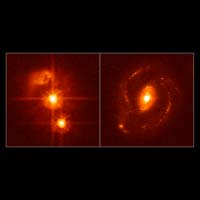
\includegraphics[max width=\linewidth]{../images/HE0450-2958.jpg}}\]
The quasar HE0450-2958 is in the middle of the left-hand picture; the
disturbed galaxy is above and a completely irrelevant foreground star is
below. For more details on what this image means, click on it.

Did this quasar begin life in the middle of a galaxy and then get kicked
out when that galaxy collided with something containing a super-massive
black hole? What could that something be?

Puzzles, puzzles, in the sky\ldots.

Closer to home, astronomers at the Keck Observatory in Hawaii have
discovered that planet Xena has a moon!
\[\href{http://www2.keck.hawaii.edu/optics/staff/mvandam/gabrielle}{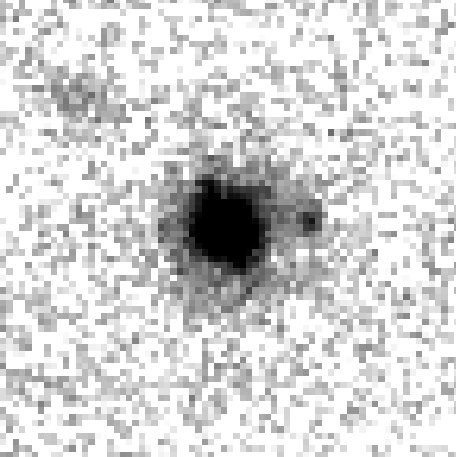
\includegraphics[max width=\linewidth]{../images/xena.jpg}}\]
They nicknamed it Gabrielle, after this famous TV character's sidekick:

\begin{enumerate}
\def\labelenumi{\arabic{enumi})}
\setcounter{enumi}{8}
\tightlist
\item
  Michael E. Brown, ``The moon of the 10th planet'',
  \texttt{http://www.gps.caltech.edu/\textasciitilde{}mbrown/planetlila/moon/index.html}
\end{enumerate}

If you hadn't heard about planet Xena, or you don't like the idea of
naming a planet after a TV character --- even a ``warrior princess'' -
don't get worked up just yet. Xena's official name is currently 2003
UB\textsubscript{313}, and though she's larger than Pluto, the
International Astronomical Union has not decided whether she'll
officially be considered a planet.

If Xena becomes a planet, she'll probably be renamed Persephone, after
the reluctant queen of the underworld in Greek mythology. But, she may
have to settle for the status of a mere ``transneptunian object'', like
Quaoar and Sedna. Indeed, if Pluto had been discovered more recently,
folks probably wouldn't have called him a planet either.

If you haven't even heard of Quaoar and Sedna\ldots{} well, you must be
too absorbed by mundane concerns to keep track of the burgeoning
population of our Solar System. But it's not too late to mend your ways!
Impress your friends by casually dropping some of this jargon:

\begin{itemize}
\item
  \href{http://en.wikipedia.org/wiki/Trans-Neptunian_object}{\textbf{Transneptunian
  object}} --- any object that orbits the Sun at an average distance
  greater than that of Neptune. Neptune is about 30 AU from the Sun,
  meaning it's 30 times farther from the Sun than we are. Transneptunian
  objects can be roughly divided into three kinds: Kuiper belt objects,
  scattered disc objects, and Oort cloud objects.
  \[\href{http://en.wikipedia.org/wiki/Kuiper_belt}{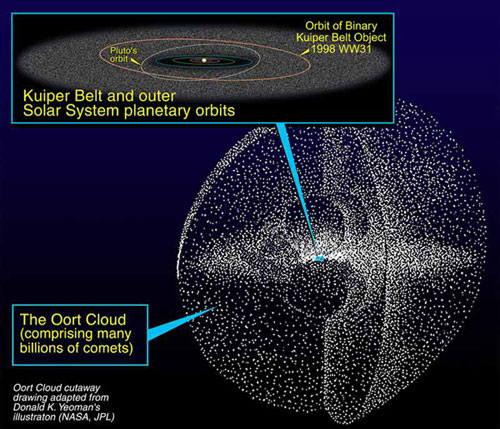
\includegraphics[max width=\linewidth]{../images/kuiper_oort.jpg}}\]

  \begin{itemize}
  \item
    \href{http://en.wikipedia.org/wiki/Kuiper_belt}{\textbf{Kuiper belt
    object}} --- any object whose orbit lies in the Kuiper belt. This is
    the region in the ecliptic (the plane of the planets' orbits)
    between 30 and 50 AU from the Sun. There are a bunch of planetoids
    in this belt. Beyond 50 AU there seems to be a sharp dropoff in
    their density. Three main kinds of Kuiper belt objects have been
    found so far: cubewanos, plutinos and twotinos.

    \begin{itemize}
    \item
      \href{http://en.wikipedia.org/wiki/Cubewano}{\textbf{Cubewano}}
      --- A cubewano is a Kuiper belt object whose orbit is not in
      resonance with any of the outer planets. The curious name comes
      from ``QB1'', since the first example was named
      \href{http://en.wikipedia.org/wiki/\%2815760\%29_1992_QB1}{1992
      QB\_1}.

      One of the biggest cubewanos is
      \href{http://en.wikipedia.org/wiki/Quaoar}{Quaoar}, with a
      diameter of about 1200 kilometers. This is about half the diameter
      of Pluto, or a third the size of the Moon: much bigger than
      anything in the asteroid belt!
      \[\href{http://en.wikipedia.org/wiki/90377_Sedna}{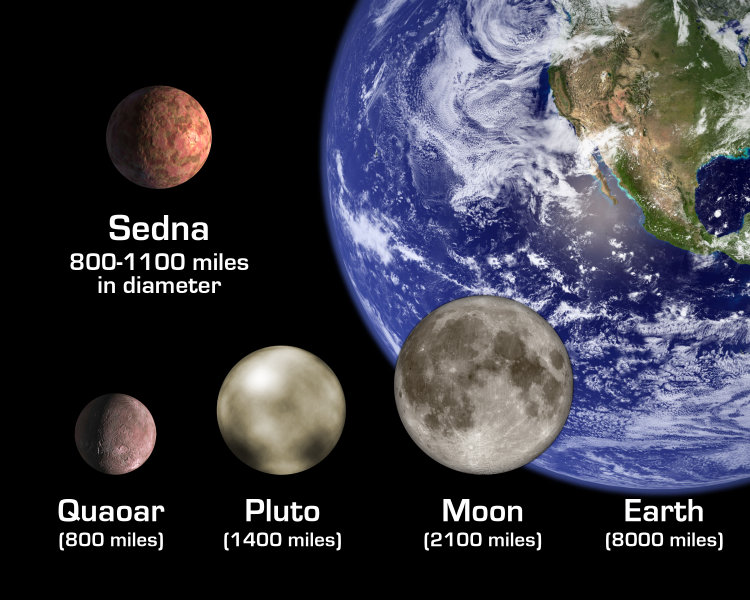
\includegraphics[max width=\linewidth]{../images/sedna.jpg}}\]
      Folks believe Quaoar is a mixture of ice and rock. It's very dark
      in color, but last year crystalline water ice was detected on its
      surface, using infrared spectroscopy. This came as a surprise,
      because cosmic rays and solar wind should convert exposed ice
      crystals to the amorphous form of ice within about 10 million
      years. Could there have been liquid water volcanos active on
      Quaoar this recently?? Or maybe meteor impacts melt amorphous ice
      and then it crystallizes?

      Other big cubewanos include
      \href{http://en.wikipedia.org/wiki/\%2819521\%29_Chaos}{Chaos},
      \href{http://en.wikipedia.org/wiki/20000_Varuna}{Varuna}, and
      \href{http://en.wikipedia.org/wiki/53311_Deucalion}{Deucalion}.
      2003 EL61 and 2005 FY9 are even bigger, but they haven't got nice
      names yet.
    \item
      \href{http://en.wikipedia.org/wiki/Plutino}{\textbf{Plutino}} ---
      A plutino is a Kuiper belt object whose orbit is in 3:2 resonance
      with Neptune: they go around the Sun twice while Neptune goes
      around three times. About a quarter of Kuiper belt objects are
      plutinos.

      The most famous plutino is
      \href{http://en.wikipedia.org/wiki/Pluto}{Pluto} itself, though
      some pedants argue that Pluto can't be a ``little Pluto''. Pluto
      is quite different than anything else we call a planet: it has an
      eccentric orbit that ranges between 30 and 50 AU, and its orbit is
      tilted 17 degrees to the ecliptic. Its surface is light brown,
      consisting mainly of frozen nitrogen and carbon monoxide. When it
      comes near the sun, as it recently did, it also gets a thin
      atmosphere made of these gases.

      Other plutinos include
      \href{http://en.wikipedia.org/wiki/28978_Ixion}{Ixion},
      \href{http://en.wikipedia.org/wiki/90482_Orcus}{Orcus},
      \href{http://en.wikipedia.org/wiki/38083_Rhadamanthus}{Rhadamanthus},
      and Pluto's moon
      \href{http://en.wikipedia.org/wiki/Charon_\%28moon\%29}{Charon}.
      If you know Greek mythology, you'll know these guys are all named
      after deities of the underworld.
    \item
      \href{http://en.wikipedia.org/wiki/Twotino}{\textbf{Twotino}} ---
      A twotino is a Kuiper belt object whose orbit is in \(2:1\)
      resonance with Neptune. These are rare compared to plutinos, and
      they're smaller, so they're stuck with boring names like 1996
      TR66. There are also a couple of Kuiper belt objects in \(4:3\)
      and \(5:3\) resonances with Neptune.
    \end{itemize}
  \item
    \href{http://en.wikipedia.org/wiki/Scattered_disc}{\textbf{Scattered
    disc object}} --- A scattered disc object is a Kuiper belt object
    that has been perturbed by interactions with Neptune into an orbit
    that is more eccentric or more tilted from the ecliptic.

    \href{http://en.wikipedia.org/wiki/2003_UB313}{Xena} (or more
    properly 2003 UB\textsubscript{313}) is a highly eccentric scattered
    disc object whose orbit carries it between 40 to 100 AU from the
    sun. Its orbit is inclined a whopping 44 degrees, and it's locked in
    a complicated \(17:5\) resonance with Neptune. It's probably larger
    than Pluto --- a reasonable rough guess is 2900 kilometers in
    diameter, as compared with 2400 for Pluto. Its surface has methane
    ice, and we now know it has a moon.

    It's quite possible that scattered disc objects are related to
    \href{http://en.wikipedia.org/wiki/Centaur_\%28planetoid\%29}{centaurs},
    which are planetoids orbiting the Sun between Jupiter and Neptune.
    The centaurs may be Kuiper belt objects that got knocked towards the
    Sun instead of away from it! Centaurs have chaotic orbits and will
    probably either collide with something or be ejected from the Solar
    System.
  \item
    \href{http://en.wikipedia.org/wiki/Oort_cloud}{\textbf{Oort cloud
    object}} --- the Oort cloud is a hypothesized spherical cloud of
    comets, perhaps between 50,000 and 100,000 AU from the Sun. The idea
    is this cloud consists of leftovers from the original nebula that
    collapsed to form our Solar system, and comets come from this region
    when they are perturbed from their orbits by the gravity of other
    stars.

    Nobody has seen a certified Oort cloud object. The best candidate so
    far is \href{http://en.wikipedia.org/wiki/90377_Sedna}{Sedna}, an
    object roughly 1500 kilometers in diameter with a wildly eccentric
    orbit taking it between 80 to 930 AU from the Sun.
    \[\href{http://en.wikipedia.org/wiki/90377_Sedna}{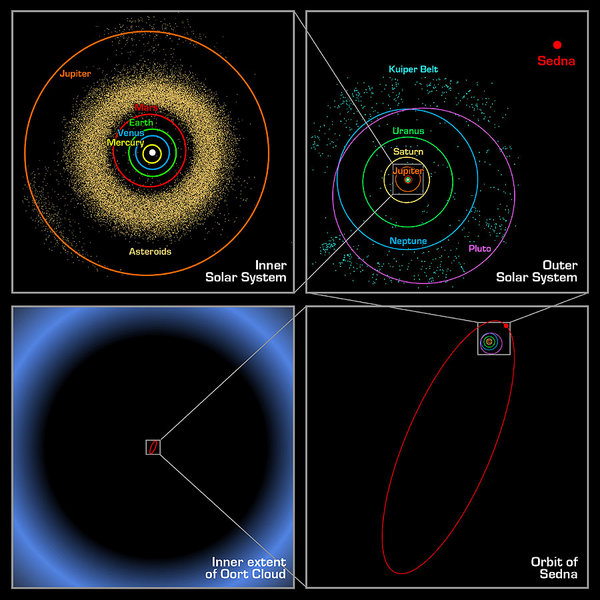
\includegraphics[max width=\linewidth]{../images/sedna_orbit.jpg}}\]
    Sedna was discovered in 2004 when it was 90 AU from the Sun. It's
    redder than Mars, its temperature never rises above 23 Kelvin, and
    its year lasts 11,250 years. It's the farthest known object in our
    Solar System, but still much closer than the Oort cloud was supposed
    to be. Maybe it's a drastic example of a scattered disc object,
    maybe it's part of an ``inner Oort cloud''\ldots{} or maybe the Oort
    cloud isn't as far out as people thought.

    The closest people have come to seeing the Oort cloud is seeing a
    ``Bok globule'':
    \[\href{http://www.eso.org/outreach/press-rel/pr-2001/pr-01-01.html}{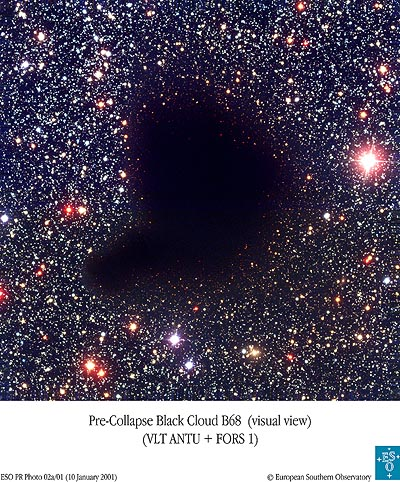
\includegraphics[max width=\linewidth]{../images/bok_globule.jpg}}\]
    A Bok globule is a cloud of dust and gas that's collapsing to form a
    star. This one is about 12,500 AU across. The scientists who
    observed it say it's about the size of the Oort cloud. This just
    goes to show how little we know about the Oort cloud!
  \end{itemize}
\end{itemize}

For a great introduction to the Kuiper belt and related topics, try
this:

\begin{enumerate}
\def\labelenumi{\arabic{enumi})}
\setcounter{enumi}{9}
\tightlist
\item
  David C. Jewitt, ``Kuiper belt'',
  \texttt{http://www.ifa.hawaii.edu/faculty/jewitt/kb.html}
\end{enumerate}

For transneptunian objects in general, try:

\begin{enumerate}
\def\labelenumi{\arabic{enumi})}
\setcounter{enumi}{10}
\tightlist
\item
  William Robert Johnston, ``Transneptunian objects'',
  \texttt{http://www.johnstonsarchive.net/astro/tnos.html}
\end{enumerate}

Also check out this newsletter:

\begin{enumerate}
\def\labelenumi{\arabic{enumi})}
\setcounter{enumi}{11}
\tightlist
\item
  \emph{Distant EKOs: the Kuiper Belt Electronic Newsletter},
  \texttt{http://www.boulder.swri.edu/ekonews/}
\end{enumerate}

Quaoar was discovered in 2002 by Chad Trujillo and Mike Brown of
Caltech:

\begin{enumerate}
\def\labelenumi{\arabic{enumi})}
\setcounter{enumi}{12}
\tightlist
\item
  Chad Trujillo, ``Quaoar'',
  \texttt{http://www.gps.caltech.edu/\textasciitilde{}chad/quaoar/}
\end{enumerate}

For evidence of crystalline water ice on Quaoar, see:

\begin{enumerate}
\def\labelenumi{\arabic{enumi})}
\setcounter{enumi}{13}
\tightlist
\item
  David C. Jewitt and Jane Luu, ``Crystalline water ice on the Kuiper
  belt object (50000) Quaoar'', \emph{Nature} \textbf{432} (2004),
  731--733. Also available at
  \texttt{http://www.ifa.hawaii.edu/faculty/jewitt/quaoar.html}
\end{enumerate}

Xena was discovered in 2003 by Trujillo, Brown and a colleague of theirs
at Yale University:

\begin{enumerate}
\def\labelenumi{\arabic{enumi})}
\setcounter{enumi}{14}
\tightlist
\item
  Michael E. Brown, Chad A. Trujillo and David L. Rabinowitz,
  ``Discovery of a planetary-sized object in the scattered Kuiper
  belt'', submitted to \emph{ApJ Letters}, available at
  \texttt{http://www.gps.caltech.edu/\%7Embrown/papers/ps/xena.pdf}
\end{enumerate}

Brown has a nice webpage about Xena and Gabrielle:

\begin{enumerate}
\def\labelenumi{\arabic{enumi})}
\setcounter{enumi}{15}
\tightlist
\item
  Michael E. Brown, ``The discovery of UB313, the 10th planet'',
  \texttt{http://www.gps.caltech.edu/\textasciitilde{}mbrown/planetlila/}
\end{enumerate}

The same gang of three also discovered Sedna in 2003:

\begin{enumerate}
\def\labelenumi{\arabic{enumi})}
\setcounter{enumi}{16}
\tightlist
\item
  Michael E. Brown, Chad A. Trujillo and David L. Rabinowitz,
  ``Discovery of a candidate inner Oort cloud planetoid'', to appear in
  \emph{ApJ Letters}, available at
  \texttt{http://www.gps.caltech.edu/\%7Embrown/papers/ps/sedna.pdf}
\end{enumerate}

\ldots{} and Brown has a fun Sedna webpage too:

\begin{enumerate}
\def\labelenumi{\arabic{enumi})}
\setcounter{enumi}{17}
\tightlist
\item
  Michael E. Brown, ``Sedna (2003 VB12)'',
  \texttt{http://www.gps.caltech.edu/\textasciitilde{}mbrown/sedna/}
\end{enumerate}

How all these transneptunian objects got where they are is a wonderful
puzzle in celestial mechanics, but you can read more about that in the
references above, especially Jewitt's Kuiper belt webpage.

Now I want to talk about Loops '05!

Instead of trying to review all the talks --- a hopeless task, since
there were 86 --- I'll just mention the \emph{two} strands of work I
find most exciting.

First, there's new evidence that a quantum theory of pure gravity
(meaning gravity without matter) makes sense in \(4\)-dimensional
spacetime.

To understand why this is exciting, you have to realize that in some
quarters, the conventional wisdom says a quantum theory of pure gravity
can't possibly make sense, except as a crude approximation at large
distance scales, because this theory is ``perturbatively
nonrenormalizable''.

Very roughly, this means that as we zoom in and look at the theory at
shorter and shorter distance scales, it looks less and less like a
``free field theory'' where gravitons zip about without interacting.
Instead, the interactions get stronger and more complicated!

So, in the jargon of the trade, we don't get a ``Gaussian ultraviolet
fixed point''.

Huh?

Well, roughly, an ``ultraviolet fixed point'' is a quantum field theory
that keeps looking the same as you keep viewing it on shorter and
shorter distance scales. A ``Gaussian'' ultraviolet fixed point is one
that's also a free quantum field theory: one where particles don't
interact.

If quantum gravity approached a Gaussian ultraviolet fixed point as we
zoomed in, we could calculate what gravitons do at arbitrarily high
energies (at least perturbatively, as power series in Newton's constant
--- no guarantee that these series converge). Particle physicists would
then be happy and say the theory was ``perturbatively renormalizable''.

But, it's not.

The conventional wisdom concludes that to save quantum gravity, we must
include matter of precisely the right sort to \emph{make} it
perturbatively renormalizable. This is the quest that led people first
to supergravity and ultimately to superstring theory --- see
\protect\hyperlink{week195}{``Week 195''} for more of this story.

But, as far back as 1979, the particle physicist Weinberg raised the
possibility that pure quantum gravity is ``nonperturbatively
renormalizable'', or ``asymptotically safe''. This means that as we zoom
in and look at the theory at shorter and shorter distance scales, it
approaches some theory \emph{other than} that of noninteracting
gravitons.

In other words, Weinberg was suggesting that pure quantum gravity
approaches a non-obvious ultraviolet fixed point --- possibly a
``non-Gaussian'' one.

The big news is that this seems to be true!

Even cooler, in this theory spacetime seems to act
\emph{\(2\)-dimensional} at very short distance scales.

This idea has been brewing for a long time --- I talked about it
extensively back in \protect\hyperlink{week139}{``Week 139''}. But now
there's more solid evidence for it, coming from two quite different
approaches.

First, people doing numerical quantum gravity in the ``causal dynamical
triangulations'' approach are seeing this effect in their computer
calculations. This is what Renate Loll explained at Loops '05. The best
place to read the details is here:

\begin{enumerate}
\def\labelenumi{\arabic{enumi})}
\setcounter{enumi}{18}
\tightlist
\item
  Jan Ambjørn, J. Jurkiewicz and Renate Loll, ``Reconstructing the
  universe'', \emph{Phys. Rev.} \textbf{D72} (2005) 064014. Also
  available as
  \href{https://arxiv.org/abs/hep-th/0505154}{\texttt{hep-th/0505154}}.
\end{enumerate}

but if you need something less technical, try this:

\begin{enumerate}
\def\labelenumi{\arabic{enumi})}
\setcounter{enumi}{19}
\tightlist
\item
  Jan Ambjørn, J. Jurkiewicz and Renate Loll, ``The universe from
  scratch'', available as
  \href{https://arxiv.org/abs/hep-th/0509010}{\texttt{hep-th/0509010}}.
\end{enumerate}

The titles of their papers are a bit grandiose, but their calculations
are solid stuff --- truly magnificent. I described their basic strategy
in my report on the Marseille conference in
\href{week206.html}{week206}. So, I won't explain that again. I'll just
mention their big new result: in pure quantum gravity, spacetime has a
spectral dimension of \(4.02\pm0.1\) on large distance scales, but
\(1.80\pm0.25\) in the limit of very short distance scales!

Zounds! What does that mean?

The ``spectral dimension'' of a spacetime is the dimension as measured
by watching heat spread out on this spacetime: the short-time behavior
of the heat equation probes the spacetime at short distance scales,
while its large-time behavior probes large distance scales. Spectral
dimensions don't need to be integers --- for fractals they're typically
not. But, Loll and company believe they're seeing spacetimes that are
\emph{exactly} \(2\)-dimensional in the limit of very small distance
scales, \emph{exactly} \(4\)-dimensional in the limit of very large
scales, with a continuous change in dimension in between. The error bars
in the above figures come from doing Monte Carlo simulations. They're
just using ordinary computers, not supercomputers. So, with more work
one could shrink their error bars and test their result.

My main worry about their work is that it uses a fixed slicing of
spactime by timelike slices. So, there's a danger that their procedure
breaks Lorentz-invariance, even in the continuum limit which they are
attempting to compute. I would like to find a way around this problem!

Luckily, some other people are getting similar results from a second
procedure that definitely does \emph{not} break Lorentz invariance:

\begin{enumerate}
\def\labelenumi{\arabic{enumi})}
\setcounter{enumi}{20}
\tightlist
\item
  Oliver Lauscher and Martin Reuter, ``Fractal spacetime structure in
  asymptotically safe gravity'', available as
  \href{https://arxiv.org/abs/hep-th/0508202}{\texttt{hep-th/0508202}}.
\end{enumerate}

Reuter spoke about all this work at Loops '05. The idea is to
investigate Weinberg's original idea in excruciatingly precise detail
using ``renormalization group flow'' ideas. The above paper is a review
of lots of others, and you need to read a bunch to get what's really
going on. The upshot, however, is that they find evidence for a
non-Gaussian ultraviolet fixed point in pure quantum gravity. Moreover,
the spectral dimension of spacetime approaches 2 in the limit of very
short distance scales.

Suppose this is all true. What does it mean?

Nobody knows yet; there are lots of attitudes one could take.

Ambjørn, Jurkiewicz and Loll could probably just plunge ahead and use
computers to calculate lots of things about quantum gravity. (Right now
they want to test their results in lots of ways.) One good thing would
be to include matter of various sorts and see how it affects the
conclusions.

Similarly, Lauscher and Reuter could just plunge ahead and compute, if
they wanted.

This is excellent. But personally, I'd like to find a beautiful theory
in which spacetime is \(2\)-dimensional at short distance scales, which
reduces to general relativity at large scales. In other words, to redo
all these calculations ``from the bottom up''.

Unsurprisingly, I hope this beautiful theory is a spin foam model, since
spin foams are \(2\)-dimensional and I like them a lot. I presented some
rough ideas on how one might invent such a model:

\begin{enumerate}
\def\labelenumi{\arabic{enumi})}
\setcounter{enumi}{21}
\tightlist
\item
  John Baez, ``Towards a spin foam model of quantum gravity'', talk at
  \emph{Loops '05}, available at
  \texttt{http://math.ucr.edu/home/baez/loops05/}
\end{enumerate}

But, these ideas are very tentative and only time will tell if they
amount to anything. What's more important is that pure quantum gravity
seems to exist --- as a theory, that is --- and people seem to be
learning actual facts about it, instead of just arguing endlessly about
it. That's progress!

The second most exciting thing at Loops '05, in my biased opinion, was
the work of John Barrett, Laurent Freidel, Karim Noui and others on
``matter without matter'' in 3d quantum gravity. Simply by carving a
Feynman-diagram-shaped hole in 3d spacetime and doing quantum gravity on
the spacetime that's left over, you get a good theory of quantum gravity
coupled to matter! You can even take the limit as Newton's gravitational
constant goes to zero and get ordinary quantum field theory on flat
spacetime!

Check these out:

\begin{enumerate}
\def\labelenumi{\arabic{enumi})}
\setcounter{enumi}{22}
\item
  John Barrett, ``Feynman diagams coupled to three-dimensional quantum
  gravity'', available as
  \href{https://arxiv.org/abs/gr-qc/0502048}{\texttt{gr-qc/0502048}}.

  John Barrett, ``Feynman loops and three-dimensional quantum gravity'',
  \emph{Mod. Phys. Lett.} \textbf{A20} (2005) 1271. Also available as
  \href{https://arxiv.org/abs/gr-qc/0412107}{\texttt{gr-qc/0412107}}.
\item
  Laurent Freidel and David Louapre, ``Ponzano-Regge model revisited I:
  gauge fixing, observables and interacting spinning particles'',
  \emph{Class. Quant. Grav.} \textbf{21} (2004) 5685--5726. Also
  available as
  \href{https://arxiv.org/abs/hep-th/0401076}{\texttt{hep-th/0401076}}.

  Laurent Freidel and David Louapre, ``Ponzano-Regge model revisited II:
  equivalence with Chern-Simons'', available as
  \href{https://arxiv.org/abs/gr-qc/0410141}{\texttt{gr-qc/0410141}}

  Laurent Freidel and Etera R. Livine, ``Ponzano-Regge model revisited
  III: Feynman diagrams and effective field theory'', available as
  \href{https://arxiv.org/abs/hep-th/0502106}{\texttt{hep-th/0502106}}.
\item
  Laurent Freidel, Daniele Oriti, and James Ryan, ``A group field theory
  for 3d quantum gravity coupled to a scalar field'', available as
  \href{https://arxiv.org/abs/gr-qc/0506067}{\texttt{gr-qc/0506067}}.
\item
  Karin Noui and Alejandro Perez, ``Three dimensional loop quantum
  gravity: coupling to point particles'', available as
  \href{https://arxiv.org/abs/gr-qc/0402111}{\texttt{gr-qc/0402111}}.
\end{enumerate}

This is mindblowingly beautiful, especially because lots of it is
already mathematically rigorous, and we can easily make more so. It's
even related to \(n\)-categories: my student Jeffrey Morton presented a
poster on this aspect.

Together with my student Derek Wise, Jeffrey Morton and I plan to have a
lot of fun studying this stuff. So, I won't talk about it more now ---
I'll probably get around to saying more someday, especially about how
the whole story generalizes to 4 dimensions.

There's a lot more to say about Loops '05, but this will have to do. In
a while, a bunch of the talks should be visible on the conference
homepage\ldots. that should give you a better idea of what happened.

\begin{center}\rule{0.5\linewidth}{0.5pt}\end{center}

\textbf{Addendum}: Here are some comments on this Week's Finds by Gene
Partlow, Phillip Helbig and Robert Helling, and my replies --- as well
as a replies by Jonathan Thornburg and Arnold Neumaier.

Gene Partlow writes:

\begin{quote}
In a recent John Baez post he mentions discovery of probably the first
known quasar found without a host galaxy. He says:

\begin{quote}
Did this quasar begin life in this galaxy and then get kicked out when
the galaxy collided with something containing a super-massive black
hole?
\end{quote}

I suggest that a fairly ordinary explanation may be that the nearby
``wildly disturbed'' galaxy may have contained several supermassive
black holes which interacted via a gravitational slingshot scenario.
This would be like a larger version of the effect where smaller mass
stars can be flung out of globular clusters when encountering larger
mass stars near the cluster center.
\end{quote}

Sounds like a possibility worth exploring. I'm no expert, so I can't
tell how likely this is. I agree that a collision with some other object
containing a super-massive black hole sounds a little odd, given that
this object --- most plausibly another galaxy --- has \emph{not been
seen}. I wouldn't have ventured such a guess myself. But, it's mentioned
on the European Southern Observatory webpage I cite above. To quote:

\begin{quote}
The absence of a massive host galaxy, combined with the existence of the
blob and the star-forming galaxy, lead us to believe that we have
uncovered a really exotic quasar, says team member Frederic Courbin
(Ecole Polytechnique Federale de Lausanne, Switzerland). ``There is
little doubt that a burst in the formation of stars in the companion
galaxy and the quasar itself have been ignited by a collision that must
haven taken place about 100 million years ago. What happened to the
putative quasar host remains unknown.''

HE0450-2958 constitutes a challenging case of interpretation. The
astronomers propose several possible explanations, that will need to be
further investigated and confronted. Has the host galaxy been completely
disrupted as a result of the collision? It is hard to imagine how that
could happen. Has an isolated black hole captured gas while crossing the
disc of a spiral galaxy? This would require very special conditions and
would probably not have caused such a tremendous perturbation as is
observed in the neighbouring galaxy.

Another intriguing hypothesis is that the galaxy harbouring the black
hole was almost exclusively made of dark matter. ``Whatever the solution
of this riddle, the strong observable fact is that the quasar host
galaxy, if any, is much too faint'', says team member Knud Jahnke
(Astrophysikalisches Institut Potsdam, Germany).
\end{quote}

Phillip Helbig writes:

\begin{quote}
John Baez writes:

\begin{quote}
Pluto is quite different than anything else we call a planet: it has an
eccentric orbit that ranges between 30 and 50 AU, and its orbit is
tilted 17 degrees to the ecliptic.
\end{quote}

Also, for a period of several years during each orbit, it is closer to
the Sun than Neptune ever is. Until relatively recently, in fact, it was
in this phase and Neptune was farther from the Sun than Pluto.
\end{quote}

Yeah! The US may still send a mission to Pluto before its atmosphere
freezes, despite delays and indecision. The ``Pluto Express'' satellite
was scheduled for launch in December 2004, but in 2000 NASA ordered a
stop-work order on the project, due to lack of money and rising cost
estimates. In 2003, Congress gave NASA money to proceed with the
project:

\begin{enumerate}
\def\labelenumi{\arabic{enumi})}
\setcounter{enumi}{26}
\tightlist
\item
  The Planetary Society, ``Pluto and Europa Campaign Page'',
  \texttt{http://www.planetary.org/html/UPDATES/Pluto/pluto\_europa\_action.html}
\end{enumerate}

and I guess it's now called ``New Horizons'':

\begin{enumerate}
\def\labelenumi{\arabic{enumi})}
\setcounter{enumi}{27}
\tightlist
\item
  ``New Horizons: NASA's Pluto-Kuiper Belt Mission'',
  \texttt{http://pluto.jhuapl.edu/}
\end{enumerate}

This webpage gives a timetable of:

\begin{itemize}
\tightlist
\item
  launch in January 2005
\item
  slingshot off Jupiter in February 2007
\item
  arrival at Pluto and Charon in July 2015
\item
  exploration of Kuiper belt during 2016-2020
\end{itemize}

I wonder if they have any plans to study the Pioneer anomaly?

Robert Helling writes:

\begin{quote}
John Baez wrote:

\begin{quote}
\begin{itemize}
\tightlist
\item
  \textbf{Twotino} --- A twotino is a Kuiper belt object whose orbit is
  in \(2:1\) resonance with Neptune. These are rare compared to
  plutinos, and they're smaller, so they're stuck with boring names like
  1996 TR66. There are also a couple of Kuiper belt objects in \(4:3\)
  and \(5:3\) resonances with Neptune.
\end{itemize}
\end{quote}

Is there an easy way to see why these resonance orbits come about? Why
do three body systems with a large central object, an intermediate
planet and a small probe happen to get the probe in resonance with the
planet? Is this just ``frequency locking happens in chaotic systems'' or
is there an easy but more quantitative way to understand this?
\end{quote}

I'm shamefully ignorant of this, so ten minutes' research on the web was
able to double my knowledge. I got ahold of this paper online:

\begin{enumerate}
\def\labelenumi{\arabic{enumi})}
\setcounter{enumi}{28}
\tightlist
\item
  B. Garfinkel, ``On resonance in celestial mechanics: a survey'',
  \emph{Celestial Mech.} \textbf{28} (1982), 275--290, also available at
  \texttt{http://adsabs.harvard.edu/cgi-bin/nph-bib\_query?bibcode=1982CeMec..28..275G}
\end{enumerate}

and while not easy to understand --- I guess there's a huge body of work
on this subject --- it uses Hamiltonian perturbation theory and
continued fractions to study resonance, and talks about a difference
between ``shallow'' and ``deep'' resonances.

The orbits of Jupiter and Saturn are almost in \(5:2\) resonance, but
this is a ``shallow'' resonance, and Saturn wiggles back and forth
around this resonance with a period of about 880 years --- an effect
called the ``Great Inequality''. The first person to study this was
Laplace. I read elsewhere that:

\begin{quote}
The dynamics of the Sun-Jupiter-Saturn system was recognized as
problematic from the beginnings of perturbation theory. The problems are
due to the so-called Great Inequality (GI), which is the Jupiter-Saturn
\(2:5\) mean-motion near-commensurability.
\end{quote}

This is from:

\begin{enumerate}
\def\labelenumi{\arabic{enumi})}
\setcounter{enumi}{29}
\tightlist
\item
  F. Varadi, M. Ghil, and W. M. Kaula, ``The great inequality in a
  planetary Hamiltonian theory'', available as
  \href{http://arxiv.org/abs/chao-dyn/9311011}{\texttt{chao-dyn/9311011}}.
\end{enumerate}

This shallow \(5:2\) resonance is related to the continued fraction
\[\frac{1}{2+\frac{1}{2+\frac{1}{14+\frac{1}{2+\ldots}}}}\] which is
close to \(2/5\).

The Pluto-Neptune \(3:2\) resonance, on the other hand, is a ``deep
resonance'' and related to the continued fraction
\[\frac{1}{2-\frac{1}{2+\frac{1}{10+\ldots}}}\] which starts out close
to \(2/3\).

I wish I understood the connection between continued fractions and
dynamical systems better! I know it gives rise to the role of the Golden
Ratio in chaos theory, which I tried to explain in
\protect\hyperlink{week203}{``Week 203''}. But, I don't understand it
very deeply.

Robert Helling also asked:

\begin{quote}
There are people doing numerical long term stability analysis of the
solar system. From what I know, they are not just taking \(F=ma\) and
Newton's law of gravity, replacing \(dt\) by \(\Delta t\) and then
integrating but use much fancier spectral methods. Could somebody please
point me to an introduction into these methods?
\end{quote}

I referred him to the work of Gerald Sussman, Jack Wisdom and others in
\protect\hyperlink{week107}{``Week 107''}, but Jonathan Thornburg posted
this reply:

\begin{quote}
I don't do this sort of work myself, but the buzzwords you want are
``symplectic ODE integrator''. The basic idea is to use an ODE
integration scheme which conserves energy, angular momentum, and maybe
other nice things, up to floating-point roundoff error, rather than just
up to finite differencing error like a standard ODE integrator would do.
\end{quote}

prompting Arnold Neumaier to give a nice list of references, which I
will take the liberty of numbering:

\begin{quote}
\begin{enumerate}
\def\labelenumi{\arabic{enumi})}
\setcounter{enumi}{30}
\tightlist
\item
  Tetsuharu Fuse, ``Planetary perturbations on the \(2:3\) mean motion
  resonance with Neptune'', \emph{Publ. Astron. Soc. Japan} \textbf{54}
  (2002), 494--499. Also available at
  \texttt{http://astronomy.nju.edu.cn/\textasciitilde{}xswan/reference/Fuse\_PASJ54\_493.pdf}
\end{enumerate}

uses symplectic integration to study \(2:3\) resonances numerically.

The thesis:

\begin{enumerate}
\def\labelenumi{\arabic{enumi})}
\setcounter{enumi}{31}
\tightlist
\item
  Luz Vianey Vela-Arevalo, \emph{Time-frequency analysis based on
  wavelets for Hamiltonian systems}, Caltech, 2002. Also available at
  \texttt{http://www.cds.caltech.edu/\textasciitilde{}luzvela/th2s.pdf}
\end{enumerate}

contains in Chapter 4 interesting numerical information about chaos,
resonances, and stability in the restricted 3-body problem. Other
interesting papers include:

\begin{enumerate}
\def\labelenumi{\arabic{enumi})}
\setcounter{enumi}{32}
\item
  George Voyatzis and John D. Hadjidemetriou, ``Symmetric and asymmetric
  librations in planetary and satellite systems at the \(2/1\)
  resonance'', available at
  \texttt{http://users.auth.gr/\textasciitilde{}hadjidem/Asymmetric1.pdf}

  Mihailo Cubrovic, ``Regimes of stability and scaling relations for the
  removal time in the asteroid belt'', available as
  \href{http://arxiv.org/abs/astro-ph/0501004}{\texttt{astro-ph/0501004}}.

  Ryszard Gabryszewski and Ireneusz Wlodarczyk, ``The resonant dynamical
  evolution of small body orbits among giant planets'', available as
  \href{http://arxiv.org/abs/astro-ph/0203182}{\texttt{astro-ph/0203182}}.

  Luz V. Vela-Arevalo and Jerrold E. Marsden, ``Time-frequency analysis
  of the restricted three-body problem: transport and resonance
  transitions'', \emph{Class. Quant. Grav.} \textbf{21} (2004),
  S351--S375. Also available at
  \texttt{http://cns.physics.gatech.edu/\textasciitilde{}luzvela/VelaArevaloMarsdenCQG\_2004.pdf}

  Harry Varvogli, Kleomenis Tsiganis, and John D. Hadjidemetriou, ``The
  `third' integral in the restricted three-body problem revisited'',
  available at
  \texttt{http://www.astro.auth.gr/\textasciitilde{}varvogli/varv5.ps}
\end{enumerate}
\end{quote}

\begin{center}\rule{0.5\linewidth}{0.5pt}\end{center}

\begin{quote}
\emph{So many worlds, so much to do,\\
So little done, such things to be.}

--- Tennyson, In Memoriam
\end{quote}



\hypertarget{week223}{%
\section{November 14, 2005}\label{week223}}

This week I'd like to talk about two aspects of higher gauge theory:
\(p\)-form electromagnetism and nonabelian cohomology. Lurking behind
both of these is the mathematics of \(n\)-categories, but I'll do my
best to hide that until the end, to build up the suspense.

But first, some cool pictures. Astronomy is booming these days, and it's
a great way to see beautiful complexity emerging from simple laws in
this wonderful universe of ours. So, I'd like the freedom to
occasionally start This Week's Finds with some pictures from the skies.
Think of it as an appetizer before the main course. Sometimes I'll
explicitly relate these pictures to math and physics; other times not.

Here's Saturn's moon Hyperion, photographed up close by the Cassini
probe:
\[\href{http://saturn.jpl.nasa.gov/multimedia/images/images.cfm?subCategoryID=29}{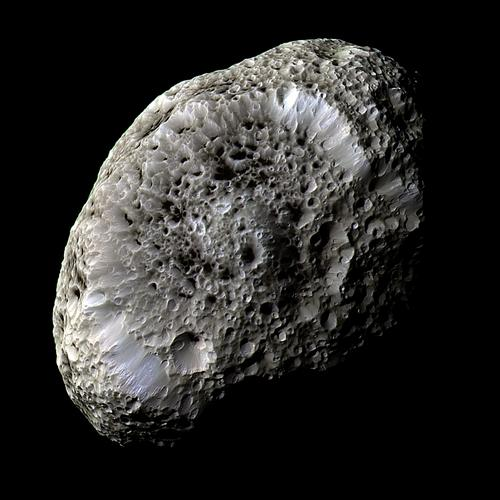
\includegraphics[max width=\linewidth]{../images/hyperion.jpg}}\]

\begin{enumerate}
\def\labelenumi{\arabic{enumi})}
\tightlist
\item
  Cassini-Huyghens Mission, ``Hyperion: Odd World'',
  \texttt{http://saturn.jpl.nasa.gov/multimedia/images/image-details.cfm?imageID=1762}
\end{enumerate}

It seems to be a huge pile of rubble loosely held together by gravity
and heavily cratered by meteor bombardments.

Hyperion is interesting because it's the only known moon that tumbles
chaotically on a short time scale, thanks to its eccentric shape and
gravitational interactions with Saturn and Titan.

This leads to some interesting math. We can think of Hyperion's angular
momentum vector as a point on a sphere. If we started out knowing this
point lay inside some small disk, time evolution would warp this disk
into an ever more complicated region as time passed. This region would
always have the same area, thanks to the wonders of symplectic geometry.
But it would sprout ever more complicated tendrils, with its perimeter
growing by a factor of e about every 100 days or so!

That's chaos for you.

Indeed, only quantum mechanics would stop the intricacy from growing
forever, by blurring it out. After about 37 years, the area of a typical
tendril would equal Planck's constant. At this point, classical
mechanics would no longer be accurate. You'd really need to describe
Hyperion's spin state using quantum theory: for example, a holomorphic
section of some line bundle on the sphere.

Well\ldots{} at least you would if it weren't for decoherence caused by
the interaction of Hyperion with its environment, for example solar
radiation! For an explanation of how this changes the story, try:

\begin{enumerate}
\def\labelenumi{\arabic{enumi})}
\setcounter{enumi}{1}
\tightlist
\item
  Michael Berry, ``Chaos and the semiclassical limit of quantum
  mechanics (is the moon there when somebody looks?)'', in \emph{Quantum
  Mechanics: Scientific Perspectives on Divine Action}, CTNS
  Publications, Vatican Observatory, 2001. Also available at
  \texttt{http://www.phy.bris.ac.uk/people/berry\_mv/the\_papers/berry337.pdf}
\end{enumerate}

Here's another great picture:
\[\href{http://heritage.stsci.edu/2004/27/index.html}{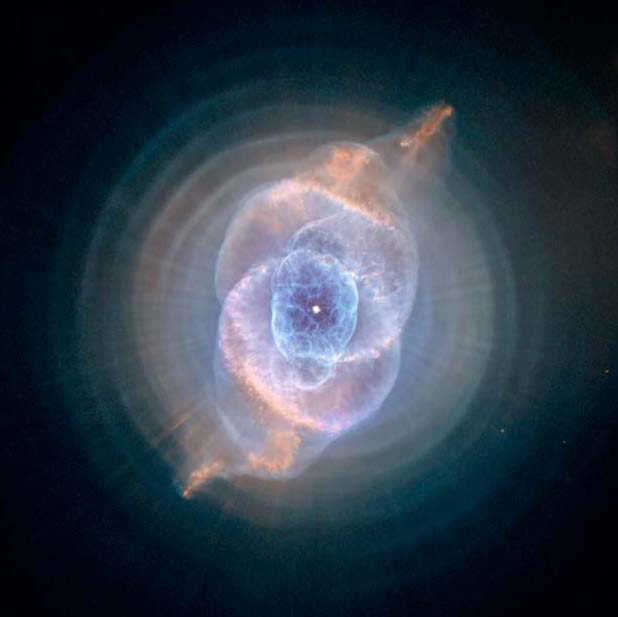
\includegraphics[max width=\linewidth]{../images/cats-eye_nebula.jpg}}\]

\begin{enumerate}
\def\labelenumi{\arabic{enumi})}
\setcounter{enumi}{2}
\tightlist
\item
  The Hubble Heritage Project, ``Cat's Eye Nebula --- NGC 6543'',
  \texttt{http://heritage.stsci.edu/2004/27/index.html}
\end{enumerate}

This is a star about the size of the Sun, nearing the end of its life,
emitting pulses of gas and dust. Astronomers call such a thing a
``planetary nebula'', though it has nothing to do with planets. It's in
our galaxy, about 3000 light years from us. When it's done shedding its
outer layers, all that's left of this star will be a white dwarf.

Our own Sun will become a planetary nebula in about 6.9 billion years,
after two separate stages of being a red giant --- one as it runs out
hydrogen, and one as it runs out of helium. When the helium is all gone,
the Sun will start to pulsate every 100,000 years, ejecting more and
more mass in each pulse, eventually throwing off all but a hot inner
core made of heavier elements. The astronomer Bruce Balick has written
eloquently on what this will mean for the Earth:

\begin{quote}
Here on Earth, we'll feel the wind of the ejected gases sweeping past,
slowly at first (a mere 5 miles per second!), and then picking up speed
as the spasms continue --- eventually to reach 1000 miles per second!!
The remnant Sun will rise as a dot of intense light, no larger than
Venus, more brilliant than 100 present Suns, and an intensely hot
blue-white color hotter than any welder's torch. Light from the fiendish
blue ``pinprick'' will braise the Earth and tear apart its surface
molecules and atoms. A new but very thin ``atmosphere'' of free
electrons will form as the Earth's surface turns to dust.
\end{quote}

So, don't keep procrastinating --- enjoy life now!

For other pictures of planetary nebulae, try Balick's webpage:

\begin{enumerate}
\def\labelenumi{\arabic{enumi})}
\setcounter{enumi}{3}
\tightlist
\item
  Bruce Balick, ``Hubble Space Telescope images of planetary nebulae'',
  \texttt{http://www.astro.washington.edu/balick/WFPC2/index.html}
\end{enumerate}

For a timeline of the universe, including the future life of our Sun,
try:

\begin{enumerate}
\def\labelenumi{\arabic{enumi})}
\setcounter{enumi}{4}
\tightlist
\item
  John Baez, ``A brief history of the universe'',
  \texttt{http://math.ucr.edu/home/baez/timeline.html}
\end{enumerate}

Now\ldots{} on to \(p\)-form electromagnetism!

In ordinary electromagnetism, the secret star of the show turns out to
be not the electromagnetic field but the ``vector potential'', \(A\). At
least locally, we can think of this as a \(1\)-form. A \(1\)-form is
just a gadget that you can integrate along a path and get a number. In
the case of the vector potential, this number describes the change in
phase that a charged particle acquires as it moves along this path.

The \(1\)-form \(A\) gives rise to a \(2\)-form \(F\) called the
``electromagnetic field''. A \(2\)-form is a gadget you can integrate
over a surface and get a number. Here's how we get \(F\) from \(A\).
Suppose we move a charged particle around a loop that's the boundary of
some surface. Then the integral of \(F\) over this surface is defined to
be the integral of \(A\) around the loop! We summarize this by saying
that \(F\) is the ``exterior derivative'' of \(A\), and writing
\[F = dA.\] \(F\) is called the electromagnetic field because\ldots{}
that's what it is! It contains both the electric and magnetic fields in
a single neat package. In 4d spacetime, the magnetic field describes the
change in a phase of a charged particle that loops around a surface in
the \(xy\), \(yz\) or \(zx\) planes. The electric field describes the
change in phase of a charged particle that loops around a surface in the
\(xt\), \(yt\) or \(zt\) planes.

If you don't know this stuff, you're missing some of the best fun life
has to offer. For an easy introduction with lots of gorgeous pictures,
see:

\begin{enumerate}
\def\labelenumi{\arabic{enumi})}
\setcounter{enumi}{5}
\tightlist
\item
  Derek Wise, ``Electricity, magnetism and hypercubes'', available at
  \texttt{http://math.ucr.edu/\textasciitilde{}derek/talks/050916bw.pdf}
\end{enumerate}

The idea of \(p\)-form electromagnetism is to replace point particles by
strings or higher-dimensional membranes. To see how this goes, it's
enough to look at \(2\)-form electromagnetism.

In \(2\)-form electromagnetism, the star of the show is a \(2\)-form,
\(A\). As already mentioned, a \(2\)-form is a gadget you can integrate
over a surface and get a number. In \(2\)-form electromagnetism, this
number describes the change in phase that a charged string acquires as
it moves along, tracing out a surface in spacetime.

The \(2\)-form \(A\) gives rise to a \(3\)-form, \(F\). A \(3\)-form is
a gadget you can integrate over a \(3\)-dimensional region and get a
number. Suppose we move a charged string and let it trace out a surface
that's the boundary of some \(3\)-dimensional region. Then the integral
of \(F\) over this region is defined to be the integral of \(A\) over
the surface! Again we write this as: \[F = dA.\] So, we're just adding
one to the dimensions of things. This makes it easy to keep on going. In
fact, for any integer \(p\), we can write down a generalization of
Maxwell's equations.

It goes like this. We start with a \(p\)-form \(A\). We define a
\((p+1)\)-form \[F = dA\] This automatically implies some of Maxwell's
equations: \[dF = 0\] but the nontrivial Maxwell equations say that
\[*d*F = J\] where \(*\) is the Hodge star operator and \(J\) is a
\(p\)-form called the ``current'', which is produced by charged matter.

What does this mean, physically? The idea is that we have charged matter
consisting of \((p-1)\)-dimensional membranes. These trace out
\(p\)-dimensional surfaces in spacetime as time passes. The current
\(J\) is a \(p\)-form that's concentrated on these surfaces. The current
affects the \(A\) field in a manner governed by Maxwell's equations.
Conversely, the \(A\) field affects the motion of the membranes.
Classically, we just integrate the \(A\) field over the surface traced
out by a membrane and add the result to the \emph{action} for the
membrane. In the path integral approach to quantum mechanics, this
number gives a change in phase, as already mentioned.

Maxwell's equations and their \(p\)-form generalization make sense when
spacetime is any Lorentzian manifold. However, to get a theory where
initial data determine a unique global solution, we want our spacetime
to be ``globally hyperbolic'', which means that it has a ``Cauchy
surface'': roughly, a spacelike surface that any sufficiently long
timelike curve hits precisely once. To get a good \emph{quantum} theory
of \(p\)-form electromagnetism with a Hilbert space of states on which
time evolution acts as unitary operators, we need more: our spacetime
should be ``stationary'', meaning that it has time translation symmetry.
Otherwise there's no way to define energy and the vacuum state --- which
is defined to be the least-energy state.

My student Miguel Carrion-Alvarez tackled an important special case in
his thesis, namely ``static'' globally hyperbolic spacetimes:

\begin{enumerate}
\def\labelenumi{\arabic{enumi})}
\setcounter{enumi}{6}
\tightlist
\item
  Miguel Carrion-Alvarez, ``Loop quantization versus Fock quantization
  of \(p\)-form electromagnetism on static spacetimes'', available as
  \href{http://arxiv.org/abs/math-ph/0412032}{\texttt{math-ph/0412032}}.
\end{enumerate}

There's a lot of interesting analysis involved, especially when space
(the Cauchy surface) is noncompact. When it's compact, we can use
``Hodge's theorem'' to relate its deRham cohomology to its topology, and
this turns out to be crucial for understanding \(p\)-form
electromagnetism --- especially issues like the \(p\)-form Bohm-Aharonov
effect. When it's noncompact we need something called ``twisted L\^{}2
cohomology'' instead, and Miguel proved a generalization of Hodge's
theorem for this.

With the analysis under control, Miguel was able to set up a very
beautiful approach to ``loop quantum electromagnetism'' and its
\(p\)-form generalization. Here the idea is to write Maxwell's equations
in terms of the integrals of \(A\) around all possible loops in space
--- or more generally, over all \(p\)-dimensional surfaces. People
interested in loop quantum gravity should like this.

As you can guess, either from seeing all the ``\(d\)'' operators or
seeing all the buzzwords I'm throwing around, \(p\)-form
electromagnetism is really just cohomology incarnated as physics! My
student Derek Wise made this very precise for a version of the theory
where spacetime is \emph{discrete} --- so-called ``lattice \(p\)-form
electromagnetism'':

\begin{enumerate}
\def\labelenumi{\arabic{enumi})}
\setcounter{enumi}{7}
\tightlist
\item
  Derek Wise, ``Lattice \(p\)-form electromagnetism and chain field
  theory'', available as
  \href{https://arxiv.org/abs/gr-qc/0510033}{\texttt{gr-qc/0510033}}.
  Version with better graphics and related material at
  \texttt{http://math.ucr.edu/\textasciitilde{}derek/pform/index.html}
\end{enumerate}

In this paper, he shows lattice \(p\)-form electromagnetism is a ``chain
field theory'': something like a topological quantum field theory, but
where what matters is not spacetime itself so much as the cochain
complex of differential forms \emph{on} spacetime, equipped with just
enough extra geometrical structure to write down the \(p\)-form version
of Maxwell's equations.

Both Miguel's thesis and Derek's papers are great if you want to learn
lots of math and physics. I seem to attract students who enjoy
explaining things.

Speaking of which\ldots.

Next I want to explain some stuff Danny Stevenson told me at a mall in
the little town of Cabazon while we were recovering from a hike in the
desert followed by pancakes at the Wheel Inn --- a roadside restaurant
famous for its
\href{http://www.bigwaste.com/photos/ca/cabazon_dinos/}{enormous statues
of dinosaurs}.

Danny works on gerbes, stacks, and higher gauge theory. Last year we
wrote a paper with Alissa Crans and Urs Schreiber constructing
\(2\)-groups (categorified groups) from the math of string theory ---
more precisely, from central extensions of loop groups. Since then I've
been spending a lot of time writing a paper with Urs on higher gauge
theory, where we set up a theory of parallel transport along surfaces.
\(2\)-form electromagnetism is the simplest case of this theory.
Meanwhile, Danny has been thinking about connections on \(2\)-vector
bundles and their relation to the cohomology of Lie \(2\)-algebras.

This has led him to generalize Schreier theory in some interesting ways.
So, let me tell you about Schreier theory!

Schreier theory is a way to classify short exact sequences of groups.
I'll say what I mean by that in a minute\ldots{} but what makes Schreier
theory special is that avoids some simplifying assumptions you might
have seen if you've studied short exact sequences before.

Normally people water down their short exact sequences by assuming some
of the groups in question are \emph{abelian}. This lets them use
``cohomology theory'' to do the classification. See
\protect\hyperlink{week210}{``Week 210''} for a nice book that takes
this approach.

This standard approach is great --- I'm not knocking it --- but Schreier
theory is more general: it's really a branch of ``nonabelian cohomology
theory''. It's not all that hard to explain, either. So, I'll explain it
and then talk about various simplifying assumptions people make.

The goal of Schreier theory is to classify short exact sequences of
groups: \[1 \to F \to E \to B \to 1\] for a given choice of \(F\) and
\(B\). ``Exact'' means that the arrows stand for homomorphisms and the
image of each arrow is the kernel of the next. Here this just means that
\(F\) is a normal subgroup of \(E\) and \(B\) is the quotient group
\(E/F\). Such a short exact sequence is also called an ``extension of
\(B\) by \(F\)'', since \(E\) is bigger than \(B\) and contains \(F\).
The simplest choice is to let \(E\) be the direct sum of \(F\) and
\(B\). Usually there are other more interesting extensions as well.

To classify these, the trick is to use the analogy between group theory
and topology.

As I explained in \protect\hyperlink{week213}{``Week 213''}, you can
think of a group as a watered-down version of a connected space with a
chosen point. The reason is that given such a space, we get a group
consisting of homotopy classes of loops based at the chosen point. This
is called the ``fundamental group'' of our space. There's a lot more
information in our space than this group. But pretty much anything you
can do for groups, you can do for such spaces. It's usually harder, but
it's completely analogous!

In particular, classifying short exact sequences is a lot like
classifying ``fibrations'': \[1 \to F \to E \to B \to 1\] where now the
letters stand for connected spaces with a chosen point, and the arrows
stand for continuous maps. If you're a physicist or geometer you may
prefer fiber bundles to ``fibrations'' --- but luckily, they're so
similar we can ignore the difference in a vague discussion like this.
The idea is basically just that \(E\) maps onto \(B\), and sitting over
each point of \(B\) we have a copy of \(F\). We call \(B\) the ``base
space'', \(E\) the ``total space'' and \(F\) the ``fiber''.

If we want to classify such fibrations we can consider carrying the
fiber \(F\) around a loop in \(B\) and see how it twists around. For
example, if all our spaces are smooth manifolds, we can pick a
connection on the total space \(E\) and see what parallel transport
around a loop in the base space \(B\) does to points in the fiber \(F\).
This gives a kind of homomorphism \[\Omega B \to \mathrm{Aut}(F)\]
sending loops in \(B\) to invertible maps from \(F\) to itself. And, the
cool thing is: this homomorphism lets us classify the fibration!

Here I say ``kind of homomorphism'' since \(\Omega B\), the space of
loops in \(B\) based at the chosen point, is only ``kind of'' a
topological group: the group laws only hold up to homotopy. But let's
not worry about this technicality --- especially since I'm being vague
about all sorts of other equally important issues!

The reason I can get away with not worrying about these issues is that
I'm trying to explain a very robust powerful principle --- one that can
easily survive a dose of vagueness that would kill a lesser idea.
Namely, if \(B\) is a connected space with a chosen basepoint,

\begin{quote}
FIBRATIONS OVER THE BASE SPACE \(B\) WITH FIBER \(F\)\\
ARE ``THE SAME'' AS\\
HOMOMORPHISMS SENDING LOOPS IN \(B\) TO AUTOMORPHISMS OF \(F\).
\end{quote}

This could be called ``the basic principle of Galois theory'', for
reasons explained in \protect\hyperlink{week213}{``Week 213''}. There I
explained the special case where the fiber is discrete. Then our
fibration called a ``covering space'', and the basic principle of Galois
theory boils down to this:

\begin{quote}
COVERING SPACES OVER \(B\) WITH FIBER \(F\)\\
ARE ``THE SAME'' AS\\
HOMOMORPHISMS FROM THE FUNDAMENTAL GROUP OF \(B\) TO AUTOMORPHISMS OF
\(F\).
\end{quote}

Okay. Now let's use the same principle to classify extensions of a group
\(B\) by a group \(F\): \[1 \to F \to E \to B \to 1\] The group \(B\)
here acts like ``loops in the base''. But what acts like ``automorphisms
of the fiber''?

You might guess it's the group of automorphisms of \(F\). But, it's
actually the \emph{\(2\)-group} of automorphisms of \(F\)!

A \(2\)-group is a categorified version of a group where all the usual
group laws hold up to natural isomorphism. They play a role in higher
gauge theory like that of groups in ordinary gauge theory. In higher
gauge theory, parallel transport along a path is described by an
\emph{object} in a \(2\)-group, while parallel transport along a
path-of-paths is described by a \emph{morphism}. In \(2\)-form
electromagnetism we use a very simple ``abelian'' \(2\)-group, which has
one object and either the real line or the circle as morphism. But there
are other more interesting ``nonabelian'' examples.

If you want to learn more about \(2\)-form electromagnetism from this
perspective, try \protect\hyperlink{week210}{``Week 210''}. For
\(2\)-groups in general, try this paper:

\begin{enumerate}
\def\labelenumi{\arabic{enumi})}
\setcounter{enumi}{8}
\tightlist
\item
  John Baez and Aaron Lauda, ``Higher-dimensional algebra V:
  \(2\)-groups'', \emph{Theory and Applications of Categories}
  \textbf{12} (2004), 423--491. Available online at
  \texttt{http://www.tac.mta.ca/tac/volumes/12/14/12-14abs.html} or as
  \href{http://arxiv.org/abs/math.QA/0307200}{\texttt{math.QA/0307200}}.
\end{enumerate}

Anyway: it turns out that any group \(F\) gives a \(2\)-group
\(\mathrm{AUT}(F)\) where the objects are automorphisms of \(F\) and the
morphisms are ``conjugations'' --- elements of \(F\) acting to conjugate
one automorphism and yield another. And, extensions
\[1 \to F \to E \to B \to 1\] are classified by homomorphisms
\[B \to \mathrm{AUT}(F)\] where we think of \(B\) as a \(2\)-group with
only identity morphisms. More precisely:

\begin{quote}
EXTENSIONS OF THE GROUP \(B\) BY THE GROUP \(F\)\\
ARE ``THE SAME'' AS\\
HOMOMORPHISMS FROM \(B\) TO THE \(2\)-GROUP \(\mathrm{AUT}(F)\)
\end{quote}

It's fun to work out the details, but it's probably not a good use of
our time together grinding through them here. So, I'll just sketch how
it works.

Starting with our extension
\[1\to F\xrightarrow{i}E\xrightarrow{p}B\to 1\] we pick a ``section''
\[E\xleftarrow{s}B\] meaning a function with \[p(s(b)) = b\] for all
\(b\) in \(B\). We can find a section because \(p\) is onto. However,
the section usually \emph{isn't} a homomorphism.

Given the section \(s\), we get a function
\[\alpha\colon B \to \mathrm{Aut}(F)\] where \(\mathrm{Aut}(F)\) is the
group of automorphisms of \(F\). Here's how:
\[\alpha(b) f = s(b) f s(b)^{-1}\] However, usually \(\alpha\)
\emph{isn't} a homomorphism.

So far this seems a bit sad: functions between groups want to be
homomorphisms. But, we can measure how much \(s\) fails to be a
homomorphism using the function \[g\colon B^2 \to F\] defined by
\[g(b,b') = s(bb') s(b')^{-1} s(b)^{-1}\] Note that \(g = 1\) iff \(s\)
is a homomorphism.

We can then use this function \(g\) to save \(\alpha\). The sad thing
about \(\alpha\) is that it's not a homomorphism\ldots{} but the good
thing is, it's a homomorphism \emph{up to conjugation by \(g\)!} In
other words:
\[\alpha(bb') f = g(b,b') [ \alpha(b) \alpha(b') f ] g(b,b')^{-1}\]
Taken together, \(\alpha\) and \(g\) satisfy some equations (``cocycle
conditions'') which say precisely that they form a homomorphism from
\(B\) to the \(2\)-group \(\mathrm{AUT}(F)\). Conversely, any such
homomorphism gives an extension of \(B\) by \(F\).

In fact, isomorphism classes of extensions of \(B\) by \(F\) correspond
in a 1-1 way with isomorphism classes of homomorphisms from \(B\) to
\(\mathrm{AUT}(F)\). So, we've classified these extensions!

In fact, something even better is true! It's evil to ``decategorify'' by
taking isomorphism classes as we did in the previous paragraph. To avoid
this, we can form a groupoid whose objects are extensions of \(B\) by
\(F\), and a groupoid whose objects are homomorphisms
\(B \to \mathrm{AUT}(F)\). I'm pretty sure that if you form these
groupoids in the obvious way, they're equivalent. And that's what this
slogan really means:

\begin{quote}
EXTENSIONS OF THE GROUP \(B\) BY THE GROUP \(F\)\\
ARE ``THE SAME'' AS\\
HOMOMORPHISMS FROM \(B\) TO THE \(2\)-GROUP \(\mathrm{AUT}(F)\)
\end{quote}

Next, let me say how Schreier theory reduces to more familiar ideas in
two special cases.

People have thought a lot about the special case where \(F\) is abelian
and lies in the center of \(E\). These are called ``central
extensions''. This is just the case where \(\alpha = 1\). The set of
isomorphism classes of central extensions is called \(H^2(B,F)\) --- the
``second cohomology'' of \(B\) with coefficients in \(F\).

People have also thought about ``abelian extensions''. That's an even
more special case where all three groups are abelian. The set of
isomorphism classes of such extensions is called \(\mathrm{Ext}(B,F)\).

Since we don't make any simplifying assumptions like this in Schreier
theory, it's part of a subject called ``nonabelian cohomology''. It was
actually worked out by Dedecker in the 1960's, based on much earlier
work by Schreier:

\begin{enumerate}
\def\labelenumi{\arabic{enumi})}
\setcounter{enumi}{9}
\item
  O. Schreier, ``Ueber die Erweiterung von Gruppen I'',
  \emph{Monatschefte fur Mathematik and Physick} \textbf{34} (1926),
  165--180. ``Ueber die Erweiterung von Gruppen II'', \emph{Abh. Math.
  Sem. Hamburg} \textbf{4} (1926), 321--346.
\item
  P. Dedecker, ``Les foncteuers \(\mathrm{Ext}_\Pi\), \(H^2_\Pi\) and
  \(H^2_\Pi\) non abeliens'', \emph{C. R. Acad. Sci. Paris} \textbf{258}
  (1964), 4891--4895.
\end{enumerate}

More recently, Schreier theory was pushed one step up the categorical
ladder by Larry Breen. As far as I can tell, he essentially classified
the extensions of a \(2\)-group B by a \(2\)-group \(F\) in terms of
homomorphisms \(B \to \mathrm{AUT}(F)\), where \(\mathrm{AUT}(F)\) is
the \emph{3-group} of automorphisms of \(F\):

\begin{enumerate}
\def\labelenumi{\arabic{enumi})}
\setcounter{enumi}{11}
\tightlist
\item
  Lawrence Breen, ``Theorie de Schreier superieure'', \emph{Ann. Sci.
  Ecole Norm. Sup.} \textbf{25} (1992), 465--514. Also available at
  \texttt{http://www.numdam.org/numdam-bin/feuilleter?id=ASENS\_1992\_4\_25\_5}
\end{enumerate}

We can keep pushing Schreier theory upwards like this, but we can also
expand it ``sideways'' by replacing groups with groupoids. You should
have been annoyed by how I kept assuming my topological spaces were
connected and equipped with a specified point. I did this to make them
analogous to groups. For example, it's for only spaces like this that
the fundamental group is powerful enough to classify covering spaces.
For more general spaces, we must use the fundamental \emph{groupoid}.
And, we can set up a Schreier theory for extensions of groupoids:

\begin{enumerate}
\def\labelenumi{\arabic{enumi})}
\setcounter{enumi}{12}
\tightlist
\item
  V. Blanco, M. Bullejos and E. Faro, ``Categorical non abelian
  cohomology, and the Schreier theory of groupoids'', available as
  \href{http://arxiv.org/abs/math.CT/0410202}{\texttt{math.CT/0410202}}.
\end{enumerate}

In fact, these authors note that Grothendieck did something similar back
in 1971: he classified \emph{all} groupoids fibered over a groupoid
\(B\) in terms of weak \(2\)-functors from \(B\) to \(\mathsf{Gpd}\),
which is the \(2\)-groupoid of groupoids! The point here is that
\(\mathsf{Gpd}\) contains \(\mathrm{AUT}(F)\) for any fixed groupoid
\(F\):

\begin{enumerate}
\def\labelenumi{\arabic{enumi})}
\setcounter{enumi}{13}
\tightlist
\item
  Alexander Grothendieck, \emph{Revêtements Étales et Groupe Fondamental
  (SGA1)}, chapter VI: ``Catégories fibrées et descente'', Lecture Notes
  in Mathematics \textbf{224}, Springer, Berlin, 1971. Also available as
  \href{http://arxiv.org/abs/math.AG/0206203}{\texttt{math.AG/0206203}}.
\end{enumerate}

Having extended the idea ``sideways'' like this, one can then continue
marching ``upwards''. I don't know how much work has been done on this,
but the slogan should be something like this:

\begin{quote}
\(n\)-GROUPOIDS FIBERED OVER AN \(n\)-GROUPOID \(B\)\\
ARE ``THE SAME'' AS\\
WEAK \((n+1)\)-FUNCTORS FROM \(B\) TO THE \((n+1)\)-GROUPOID
\(n\mathsf{Gpd}\)
\end{quote}

Grothendieck also studied this kind of thing with categories replacing
groupoids, so there should also be an \(n\)-category version, I
think\ldots{} but it's more delicate to define ``fibrations'' for
categories than for groupoids, so I'm a bit scared to state a slogan
suitable for \(n\)-categories.

However, I'm not scared to go from \(n\)-groupoids to
\(\omega\)-groupoids, which are basically the same as spaces. In terms
of spaces, the slogan goes like this:

\begin{quote}
SPACES FIBERED OVER THE SPACE \(B\)\\
ARE ``THE SAME'' AS\\
MAPS FROM \(B\) TO THE SPACE OF ALL SPACES
\end{quote}

This is how James Dolan taught it to me. Most mortals are scared of
``the space of all spaces'' --- both for fear of Russell's paradox, and
because we really need a \emph{space} of all spaces, not just a mere set
of them. To avoid these terrors, you can water down Jim's slogan by
choosing a specific space \(F\) to be the fiber:

\begin{quote}
FIBRATIONS WITH FIBER \(F\) OVER THE SPACE \(B\)\\
ARE ``THE SAME'' AS\\
MAPS FROM \(B\) TO THE CLASSIFYING SPACE OF \(\mathrm{AUT}(F)\)
\end{quote}

where \(\mathrm{AUT}(F)\) is the topological group of homotopy
self-equivalences of \(F\). The fearsome ``space of all spaces'' is then
the disjoint union of the classifying spaces of all these topological
groups \(\mathrm{AUT}(F)\). It's too large to be a space unless you pass
to a larger universe of sets, but otherwise it's perfectly fine.
Grothendieck invented the notion of a ``Grothendieck universe'' for
precisely this purpose:

\begin{enumerate}
\def\labelenumi{\arabic{enumi})}
\setcounter{enumi}{14}
\tightlist
\item
  Wikipedia, ``Grothendieck universe'',
  \texttt{http://en.wikipedia.org/wiki/Grothendieck\_universe}
\end{enumerate}

\begin{center}\rule{0.5\linewidth}{0.5pt}\end{center}

\textbf{Addendum:} I'd like to thank Leo Alonso for pointing out that
Grothendieck's famous ``SGA1'' is now available on the arXiv in TeX
form, courtesy of the Société Mathématique de France. SGA2 is also
available on the arXiv, and more are coming.

Here are further addenda thanks to Kevin Buzzard, Toby Bartels, David
Corfield, Peter May, Jim Stasheff, and Ronnie Brown.

First, an email I sent in reply to Kevin Buzzard, who was curious about
how we classify extensions of the group \(B\) by the group \(F\) using
homomorphisms from \(B\) to the \(2\)-group \(\mathrm{AUT}(F)\). In
particular, he wanted to know the definition of ``\(2\)-group'' and
``homomorphism between \(2\)-groups'', and how \(\mathrm{AUT}(F)\) is
defined:

\begin{quote}
Dear Kevin -

You write:

\begin{quote}
I'm just checking some of the details (extensions of groups are
morphisms of \(2\)-groups) and I find that you've not given me quite
enough information to do it (in the sense that I'm not knowledgeable
enough about standard facts about \(2\)-groups to fill in some of the
details that you allude to).
\end{quote}

Sorry. I'm glad you care enough to want to know this stuff: \(2\)-groups
and homomorphisms between them are defined in loving detail in
\href{http://arxiv.org/abs/math.QA/0307200}{my paper with Aaron Lauda},
but I'll answer your questions here and append this to
\protect\hyperlink{week223}{``Week 223''} to help out anyone else who
cares.

\begin{quote}
Say we're in the ``classical'' case where \(F\) is an abelian group,
\(B\) is a group, and we're classifying extensions
\(1\to F\to E\to B\to1\) where \(F\) lies in the centre of \(E\). We
know the answer here: such \(E\)'s are classified by \(H^2(B,F)\) which,
for me, means \(2\)-cocycles over \(2\)-coboundaries. Recall that a
\(2\)-cocycle is \(g\colon B^2\to F\) satisfying
\(g(a,bc)+g(b,c)=g(a,b)+g(ab,c)\).
\end{quote}

Right.

\begin{quote}
You want the answer to be homomorphisms \(B \to \mathrm{AUT}(F)\). You
don't quite give the definitions of these things.
\end{quote}

True. Let me start by saying what a \(2\)-group is, and then how the
group \(B\) becomes a \(2\)-group, and then how \(\mathrm{AUT}(F)\) is
defined.

A group is just a category with one object and with all morphisms
invertible. Slick! But, we usually prefer to think of a group as a set:
the morphisms of our category get called ``elements'' of this set. This
set then has a multiplication function \[m\colon G \times G \to G\] and
an identity element \[1 \in G\] satisfying the associative and unit
laws, and such that every element has an inverse.

All this categorifies painlessly:

A \(2\)-group is just a \(2\)-category with one object and with all
morphisms and \(2\)-morphisms invertible. Slick! But, we sometimes
prefer to think of a \(2\)-group as a category: the morphisms of our
\(2\)-category get called ``objects'' of this category, and the
\(2\)-morphisms get called ``morphisms''. This category then has a
multiplication functor \[m\colon G \times G \to G\] and an identity
object \[1 \in G\] satisfying the associative and unit laws, and such
that every object and morphism has an inverse.

In short: a \(2\)-group is just like a group, but with the word
``category'' replacing the word ``set'', the word ``object'' replacing
the word ``element'', and so on!

Now, how does a group become a \(2\)-group? Simple: we take the
\emph{elements} of our group and make them the \emph{objects} of our
\(2\)-group; then we say the only morphisms of our \(2\)-group are
identity morphisms. The \(2\)-group multiplication
\(m\colon G \times G \to G\) comes from the multiplication in our group,
and so on.

\begin{quote}
Let's stick to \(F\) abelian. You think of \(\mathrm{AUT}(F)\) as being
the \(2\)-category with objects \(\mathrm{Aut}(F)\), \(1\)-morphisms
\(\mathrm{Hom}(\varphi,\psi)=F\) if \(\varphi=\psi\) and empty otherwise
(because \(F\) is abelian). What are the \(2\)-morphisms? Is
\(\mathrm{Hom}(\varphi,\psi)\) supposed to be a category with objects
\(F\)?
\end{quote}

Alas, you're one dimension down: thought of as a \(2\)-category, we want
our \(2\)-group \(\mathrm{AUT}(F)\) to have one object, the usual group
\(\mathrm{Aut}(F)\) as morphisms, and conjugations between these as
\(2\)-morphisms.

Here's how we get this. Think of our group \(F\) as a category. Then let
\(\mathrm{AUT}(F)\) have \(F\) as its only object, invertible functors
\[a\colon F \to F\] as its morphisms, and natural isomorphisms between
these as its \(2\)-morphisms.

That's very slick. But let me say this in a different way using the
other viewpoint, where we think of a \(2\)-group as a ``category with
multiplication and inverses''. Given a group \(F\), our \(2\)-group
\(\mathrm{AUT}(F)\) will be the category where the objects are
automorphisms \[a\colon F \to F\] and where a morphism
\(f\colon a \to a'\) is an element \(f\) of \(F\) that conjugates \(a\)
to give \(a'\): \[f a(g) f^{-1} = a'(g) \quad\mbox{for all $g \in F$}\]
This viewpoint requires some extra work to check that
\(\mathrm{AUT}(F)\) is a \(2\)-group. The \(2\)-category viewpoint is
actually much more efficient.

\begin{quote}
Now what is a homomorphism \(B \to \mathrm{AUT}(F)\)?
\end{quote}

Here's where the subtlety comes in: weakening! So far we haven't
weakened anything: all the equations in the definition of a group became
equations in the definition of a \(2\)-group. We're really just dealing
with ``strict'' \(2\)-groups here. But we need to \emph{weaken} the
definition of homomorphism, replacing some equations by isomorphisms, to
get things to work out well now.

If we think of \(B\) and \(\mathrm{AUT}(F)\) as \(2\)-categories, a
homomorphism \(B \to \mathrm{AUT}(F)\) is just a weak \(2\)-functor.
Slick! But, you may not enjoy this definition as much as I do.

So, let's think of \(B\) and \(\mathrm{AUT}(F)\) as ``categories with
multiplication and inverses''. Then a homomorphism
\[\alpha\colon B \to \mathrm{AUT}(F)\] is a functor that preserves
multiplication of objects \emph{up to a specified isomorphism}, which
must satisfy some laws of its own.

Quite roughly, this means that given two objects \(b\) and \(b'\) of
\(B\), we don't have an equation \[\alpha(bb') = \alpha(b) \alpha(b')\]
Instead, we have an isomorphism
\[g(b,b')\colon \alpha(bb') \to \alpha(b) \alpha(b')\] This needs to
satisfy some equations. I can tell you these if you want, but for
starters you can check that in our application, this \(g(b,b')\) thing
will be the \(2\)-cocycle familiar from group cohomology!

And, the laws \(g\) must satisfy say precisely that \(g\) is a
\(2\)-cocycle.

(Indeed, for a \emph{central} extension \(\alpha = 1\), so all we really
need to think about is this \(2\)-cocycle \(g\). Schreier theory goes on
to consider more general extensions, where \(\alpha \neq 1\).)

\begin{quote}
I'm sure I could just go and read Breen's book, but these questions are
so trivial that I'm sure you can instantly answer them, and you also get
the confirmation that there are still people out there reading TWF.
\end{quote}

That's worth a lot! If you ever want to learn more about \(2\)-groups
and homomorphisms between them, I think
\href{http://arxiv.org/abs/math.QA/0307200}{my paper with Aaron Lauda}
could be easier than
\href{http://www.numdam.org/numdam-bin/feuilleter?id=ASENS_1992_4_25_5}{Breen's
opus}. Breen's opus concerns ``higher Schreier'' theory --- classifying
extensions of \(2\)-groups with the help of \(3\)-groups!

Best,\\
jb
\end{quote}

It's important to note that it's \emph{isomorphism classes} of
extensions that correspond to \emph{isomorphism classes} of
homomorphisms \(B \to \mathrm{Aut}(F)\). For this, one needs to know
what a ``\(2\)-isomorphism'' between homomorphisms of \(2\)-groups is.
Again, this is explained in my paper with Lauda. It's a special case of
a weak natural isomorphism between weak \(2\)-functors between
\(2\)-categories, but we say what this means in terms that working
mathematicians can understand.

Also, Toby Bartels had some comments on the dinosaurs of Cabazon and
size issues in category theory:

\begin{quote}
John wrote in part:

\begin{quote}
Next I want to explain some stuff Danny Stevenson told me at a mall in
the little town of Cabazon while we were recovering from a hike in the
desert followed by pancakes at the Wheel Inn --- a roadside restaurant
famous for its enormous statues of dinosaurs.
\end{quote}

Did you see
\href{http://www.latimes.com/news/local/la-me-dinosaurs27aug27,0,3988775,full.story}{the
creationist sign by the dinosaurs?}

\begin{quote}
SPACES FIBERED OVER THE SPACE \(B\) ARE ``THE SAME'' AS MAPS FROM \(B\)
TO THE SPACE OF ALL SPACES
\end{quote}

\begin{quote}
The fearsome ``space of all spaces'' is then the disjoint union of the
classifying spaces of all these topological groups \(\mathrm{AUT}(F)\).
It's too large to be a space unless you pass to a larger universe of
sets, but otherwise it's perfectly fine.
\end{quote}

So if you want your slogan to treat size issues carefully:

\begin{quote}
SPACES FIBERED OVER THE SPACE \(B\)\\
ARE ``THE SAME'' AS\\
MAPS FROM \(B\) TO THE SPACE OF ALL SMALL SPACES
\end{quote}

But you were secretly doing this all along! After all, when you wrote:

\begin{quote}
\(n\)-GROUPOIDS FIBERED OVER AN \(n\)-GROUPOID \(B\) ARE ``THE SAME'' AS
WEAK \((n+1)\)-FUNCTORS FROM \(B\) TO THE \((n+1)\)-GROUPOID
\(n\mathsf{Gpd}\)
\end{quote}

you simply used ``\(n\mathsf{Gpd}\)'' to abbreviate ``OF ALL SMALL
\(n\)-GROUPOIDS''. So there are really no new size issues at the
\(\omega\) level.

(Exercise for those that like this sort of thing: Do we need to state
that \(B\) and \(F\) are small?)

-- Toby
\end{quote}

Thanks for clearing this up. I prefer not to distract people with size
issues, so I didn't mention them until ``the space of all spaces''
walked in the door, at which point I figured alarm bells would start
ringing for lots of people. But, it was already hiding in the ``the
\((n+1)\)-groupoid of all \(n\)-groupoids''. I prefer to use a new
Grothendieck universe for each level of the \(n\)-categorical hierarchy,
to justify such expressions. I guess \(\omega\)-categories then require
an \(\omega\)-th universe.

Yes, I saw that silly sign in front of the dinosaurs, though I didn't
understand its full meaning until now. It wasn't there the last time I
visited. Apparently the new owners have decided to enlist this nice
roadside attraction as part of the propaganda campaign for creationism.
They actually believe Adam and Eve walked with dinosaurs in Eden --- as
one biologist put it, ``they think The Flintstones is a documentary''.

It's sad how just as the magnificent history of the universe is becoming
vividly clear, some want to truncate it to a pitifully human scale ---
and then claim \emph{that} was God's work.

Next, David Corfield had some questions about the ``space of all
spaces'', which I answered in this email:

\begin{quote}
Dear David -

You wrote:

\begin{quote}
Hi,

\begin{quote}
SPACES FIBERED OVER THE SPACE \(B\) ARE ``THE SAME'' AS MAPS FROM \(B\)
TO THE SPACE OF ALL SMALL SPACES
\end{quote}

Is there another handle on this, other than

\begin{quote}
OMEGA-GROUPOIDS FIBERED OVER THE OMEGA-GROUPOID \(B\) ARE ``THE SAME''
AS WEAK OMEGA-FUNCTORS FROM \(B\) TO THE OMEGA-GROUPOID OF ALL SMALL
OMEGA-GROUPOIDS ?
\end{quote}

Presumably \(B\) must be small, and the spaces fibered over it.
\end{quote}

It suffices for the fibers to be small, so if you want a really nitpicky
motto:

\begin{quote}
SMALL \(\omega\)-GROUPOIDS FIBERED OVER THE \(\omega\)-GROUPOID \(B\)\\
ARE ``THE SAME'' AS\\
WEAK \(\omega\)-FUNCTORS FROM \(B\) TO THE \(\omega\)-GROUPOID OF ALL\\
SMALL \(\omega\)-GROUPOIDS\\
\end{quote}

\begin{quote}
Do you and Jim have other intuitions about THE SPACE OF ALL SMALL
SPACES?
\end{quote}

One can describe it in a completely precise and rigorous way. It's the
disjoint union over all homotopy types of small spaces \(F\) of the
classifying spaces \(B(\mathrm{Aut}(F))\). Here \(\mathrm{Aut}(F)\) is
the topological group of homotopy self-equivalences of \(F\).

Note: the ``largeness'' of this space is solely due to it being a
disjoint union of a proper class of connected components. When we map
any small space to it, the map can only hit a set's worth of components.
So, it's not really scary.

And, if we map a connected small space \(X\) to it, we get a map
\[X \to B(\mathrm{Aut}(F))\] for some \(F\), which is just what you need
to get an \(F\)-bundle over \(X\).

\begin{quote}
Like, is it one of your FREE SUCH-AND-SUCHES?
\end{quote}

I don't know a description like that offhand, since ``free'' suggests a
left universal property, and the space of all (small) spaces mainly has
a right universal property, which describes maps \emph{into} it.

Namely: maps from \(X\) into the space of all spaces are ``the same as''
fibrations over \(X\).

I could make this completely precise, but it's probably not worth
bothering here; one just needs suitable equivalence relations.
\end{quote}

Next, Peter May wrote:

\begin{quote}
In his posting today, John Baez advertised the slogan:

\begin{quote}
FIBRATIONS OVER THE BASE SPACE \(B\) WITH FIBER \(F\)\\
ARE ``THE SAME'' AS\\
HOMOMORPHISMS SENDING LOOPS IN \(B\) TO AUTOMORPHISMS OF \(F\).
\end{quote}

He hedged it with a ``dose of vagueness'', but in fact I proved a
completely precise and general version of exactly this result in:

\begin{enumerate}
\def\labelenumi{\arabic{enumi})}
\setcounter{enumi}{15}
\tightlist
\item
  Peter May, ``Classifying spaces and fibrations'', \emph{Memoirs AMS}
  \textbf{155}, Jan.~1975.
\end{enumerate}

Using Moore loops on \(B\), \(LB\), one has a topological monoid, and
one also has the topological monoid \(\mathrm{Aut}(F)\) of homotopy
equivalences of \(F\). A ``transport'' is a homomorphism of topological
monoids from \(LB\) to \(\mathrm{Aut}(F)\). Allowing \(F\) to vary by a
homotopy equivalence, one can define an equivalence relation on
transports such that the equivalence classes are in natural bijective
correspondence with the equivalence classes of ``fibrations over the
base space \(B\) with fiber \(F\)''. One can generalize the context by
allowing fibers in some nice category and prove the same result. See
opus cit, Theorem 14.2, page 83. That was over 30 years ago, so
naturally I wasn't thinking about categorification, but I would imagine
that the methods categorify.
\end{quote}

Here and below I've taken the liberty of numbering the references to
papers, so it's easier to find them in my table of contents for This
Week's Finds.

Jim Stasheff wrote:

\begin{quote}
Even more ancient:

\begin{enumerate}
\def\labelenumi{\arabic{enumi})}
\setcounter{enumi}{16}
\tightlist
\item
  James Stasheff, ``Parallel transport in fibre spaces'', \emph{Bol.
  Soc. Mat. Mexicana} (1968), 68--86.
\end{enumerate}

Unfortunately that's a hard paper to get a hold of.

Somewhat related is:

\begin{enumerate}
\def\labelenumi{\arabic{enumi})}
\setcounter{enumi}{17}
\tightlist
\item
  James Stasheff, ``Associated fibre spaces'', \emph{Michigan Math.
  Journal} \textbf{15} (1968), 457--470.
\end{enumerate}

and at the survey level:

\begin{enumerate}
\def\labelenumi{\arabic{enumi})}
\setcounter{enumi}{18}
\tightlist
\item
  James Stasheff, ``H-spaces and classifying spaces, I-IV'', \emph{AMS
  Proc. Symp. Pure Math.} \textbf{22} (1971), 247--272.
\end{enumerate}

Of course, as you might expect, I describe things in terms of
\(A_\infty\)-morphisms from the space of loops into \(\mathrm{Aut}(F)\)
of homotopy equivalences of \(F\).

Now that some of us are comfortable with \(A_\infty\)-cats,
categorification should proceed, perhaps with some technical details.

jim
\end{quote}

Ronnie Brown wrote:

\begin{quote}
John Baez gave an interesting account of nonabelian cohomology and
extension theory. Here are a few more references with which I have been
involved, all using crossed complexes and free crossed resolutions:

\begin{enumerate}
\def\labelenumi{\arabic{enumi})}
\setcounter{enumi}{19}
\tightlist
\item
  Ronald Brown and P. J. Higgins, ``Crossed complexes and non-abelian
  extensions'', \emph{Category theory proceedings, Gummersbach, 1981},
  (ed.~K.H. Kamps et al) Lecture Notes in Math. \textbf{962} Springer,
  Berlin, 1982, pp.~39--50.
\end{enumerate}

This generalises classical Schreier theory to extensions of groupoids.

\begin{enumerate}
\def\labelenumi{\arabic{enumi})}
\setcounter{enumi}{20}
\tightlist
\item
  Ronald Brown and O. Mucuk, ``Covering groups of non-connected
  topological groups revisited'', \emph{Math. Proc. Camb. Phil. Soc.}
  \textbf{115} (1994) 97--110. Also available as
  \href{http://arxiv.org/abs/math.AT/0009021}{\texttt{math.AT/0009021}}.
\end{enumerate}

This relates the theory of covering topological groups of non connected
topological groups to the classical theory of extensions and
obstructions to a \(Q\)-kernel with an invariant in \(H3\). It uses the
properties of the internal hom in crossed complexes
\(\mathrm{CRS}(F,C)\), and exact sequences derived from a fibration
\(C \to D\) and the induced fibration on \(\mathrm{CRS}(F,-)\).

\begin{enumerate}
\def\labelenumi{\arabic{enumi})}
\setcounter{enumi}{21}
\tightlist
\item
  Ronald Brown and Timothy Porter, ``On the Schreier theory of
  non-abelian extensions: generalisations and computations'',
  \emph{Proceedings Royal Irish Academy} \textbf{96A} (1996), 213--227.
  Also available at
  \texttt{http://www.informatics.bangor.ac.uk/public/math/research/ftp/algtop/rb/nonabex4.ps.gz}
\end{enumerate}

This establishes a generalisation of the Schreier theory in two ways
(but only for groups). One is using coefficients in a crossed module,
following Dedecker's key ideas, as in the references in John's account.
Second it shows how to compute with such extensions \[A \to E \to G\] in
terms of presentations of the group \(G\). This involves identities
among relations for the presentation, as shown originally by Turing in

\begin{enumerate}
\def\labelenumi{\arabic{enumi})}
\setcounter{enumi}{22}
\tightlist
\item
  Alan Turing, ``The extensions of a group'', \emph{Compositio
  Mathematica} \textbf{5} (1938), 357--367.
\end{enumerate}

The advantage of this method is that one can actually do sums, even when
the group \(G\) may be infinite. The example given by us is \(G\) =
trefoil group with two generators \(x,y\) and relation \(x^3=y^2\). This
presentation has no identities among relations, and so the calculation
is especially simple. Equivalence of extensions is described in terms of
homotopies of morphisms of crossed complexes, and this relates the ideas
to other forms of homological or homotopical algebra.

An advantage of this approach is the ability to calculate some small
free crossed resolutions of some groups: this is one reason for using
crossed complexes. Note that a convenient monoidal closed structure on
the category of crossed complexes has been explicitly written down, and
this allows convenient calculation and representations of homotopies,
using the `unit interval' groupid, as a crossed complex.

One of the problems I have with the globular approach is the difficulty
of writing down homotopies, and higher homotopies. For example, Ilhan
Icen and I found it difficult to rewrite in terms of group-groupoids the
well known Whitehead theory of automorphisms of crossed modules,
explained for the crossed modules of groupoids case in:

\begin{enumerate}
\def\labelenumi{\arabic{enumi})}
\setcounter{enumi}{23}
\tightlist
\item
  Ronald Brown and Ilhan Icen, ``Homotopies and automorphisms of crossed
  modules of groupoids'', \emph{Applied Categorical Structures}
  \textbf{11} (2003) 185--206. Also available as
  \href{http://arxiv.org/abs/math.CT/0008117}{\texttt{math.CT/0008117}}.
\end{enumerate}

It looks as if it would be better expressed in terms of automorphisms of
\(2\)-groupoids: good marks to anyone who writes it down in that way!

One knows such homotopies of globular \(\infty\)-groupoids exist because
globular \(\infty\)-groupoids are equivalent to crossed complexes:

\begin{enumerate}
\def\labelenumi{\arabic{enumi})}
\setcounter{enumi}{24}
\tightlist
\item
  Ronald Brown and P. J. Higgins, ``The equivalence of
  \(\infty\)-groupoids and crossed complexes'', \emph{Cah. Top. Geom.
  Diff.} \textbf{22} (1981) 371--386.
\end{enumerate}

(This paper contains an early definition of a (strict, globular)
\(\infty\) category.)

This raises a question: what is the crossed complex associated to the
free globular groupoid on one generator of dimension \(n\)? I have a
round-about sketch proof, using also cubical theory, and a van Kampen
theorem, that it \emph{is} the fundamental crossed complex of the
\(n\)-globe. Does anyone have a purely algebraic proof?

The idea of singular nonabelian cohomology of a space \(X\) with
coefficients in a crossed complex \(C\) is given in:

\begin{enumerate}
\def\labelenumi{\arabic{enumi})}
\setcounter{enumi}{25}
\tightlist
\item
  Ronald Brown and P. J. Higgins, ``The classifying space of a crossed
  complex'', \emph{Math. Proc. Camb. Phil. Soc.} \textbf{110} (1991)
  95--120.
\end{enumerate}

This cohomology is given by \([\Pi SX, C]\), homotopy classes of maps
from the fundamental crossed complex of the singular complex of \(X\),
to \(C\). There is also a Cech version (current work with Jim Glazebrook
and Tim Porter).

An interesting problem is to classify extensions of crossed complexes!

There is an interesting account of extensions of principal bundles and
transitive Lie groupoids by Androulidakis, developing work of Mackenzie,
at:

\begin{enumerate}
\def\labelenumi{\arabic{enumi})}
\setcounter{enumi}{26}
\tightlist
\item
  Iakovos Androulidakis, ``Classification of extensions of principal
  bundles and transitive Lie groupoids with prescribed kernel and
  cokernel'', \emph{J. Math. Phys.} \textbf{45} (2004), 3095--4012. Also
  available as
  \href{http://arxiv.org/abs/math.DG/0402007}{\texttt{math.DG/0402007}}.
\end{enumerate}

(not using crossed complexes).

Ronnie Brown\\
\texttt{http:www.bangor.ac.uk/r.brown}
\end{quote}

Finally, here's my reply to a bemused comment by Jim Stasheff:

\begin{quote}
Jim Stasheff wrote:

\begin{quote}
John and anyone else who cares to weigh in, here are some comments from
the purely topological or rather homotopy theory side:
\end{quote}

\begin{quote}
For both bundles and fibrations (e.g.~over a paracompact base), your
last slogan is the oldest:
\end{quote}

\begin{quote}
FIBRATIONS WITH FIBER \(F\) OVER THE SPACE \(B\) ARE ``THE SAME'' AS
MAPS FROM \(B\) TO THE CLASSIFYING SPACE OF \(\mathrm{AUT}(F)\)
\end{quote}

\begin{quote}
``the same as'' referring to homotopy classes.
\end{quote}

It's certainly old, but I mentioned another that may be older:

\begin{quote}
COVERING SPACES OF \(B\) WITH FIBER \(F\)\\
ARE ``THE SAME'' AS\\
HOMOMORPHISMS FROM THE FUNDAMENTAL GROUP OF \(B\) TO AUTOMORPHISMS OF
\(F\)
\end{quote}

although one usually sees this special case (which I didn't bother to
mention):

\begin{quote}
CONNECTED COVERING SPACES OF \(B\) WITH FIBER \(F\)\\
ARE ``THE SAME'' AS\\
TRANSITIVE ACTIONS OF THE FUNDAMENTAL GROUP OF \(B\) ON \(F\)
\end{quote}

which is usually disguised as follows:

\begin{quote}
CONNECTED COVERING SPACES OF \(B\)\\
ARE ``THE SAME'' AS\\
SUBGROUPS OF THE FUNDAMENTAL GROUP OF \(B\)
\end{quote}

Anyway, I wasn't trying to present things in historical order. I was
trying present them roughly in order of increasing ``dimension'',
starting with extensions of groups, then going up to \(2\)-groups, then
expanding out to groupoids, then going up to \(n\)-groupoids, and
finally \(\omega\)-groupoids\ldots{} which are the same as homotopy
types!

And here, as usual, the \(n\)-category theorists meet up with the
topologists --- and find that the topologists have already done
everything there is to do with \(\omega\)-groupoids \ldots{} but usually
by thinking of them of them as \emph{spaces}, rather than
\(\omega\)-groupoids!

It's sort of like climbing a mountain, surmounting steep cliffs with the
help of ropes and other equipment, and then finding a Holiday Inn on top
and realizing there was a 4-lane highway going up the other side.

So, as usual, the main point of calling homotopy types
``\(\omega\)-groupoids'' instead of ``spaces'' is not to reinvent
topology, but to see how ideas from topology generalize to
\(n\)-category theory. Think of spaces as \(\omega\)-groupoids, but use
those as a springboard for \(\omega\)-categories --- or at least
\(n\)-categories, perhaps just for low values of \(n\) if one is feeling
tired.

In the case at hand, the \(\omega\)-groupoidal slogan:

\begin{quote}
FIBRATIONS OF \(\omega\)-GROUPOIDS WITH FIBER \(F\) AND BASE \(B\)\\
ARE ``THE SAME'' AS\\
WEAK \(\omega\)-FUNCTORS FROM \(B\) TO \(\mathrm{AUT}(F)\)
\end{quote}

is just a reformulation of:

\begin{quote}
FIBRATIONS WITH FIBER \(F\) OVER THE SPACE \(B\)\\
ARE ``THE SAME'' AS\\
MAPS FROM \(B\) TO THE CLASSIFYING SPACE OF \(\mathrm{AUT}(F)\)
\end{quote}

but it suggests a grandiose generalization:

\begin{quote}
FIBRATIONS OF \(\omega\)-CATEGORIES WITH BASE \(B\)\\
ARE ``THE SAME'' AS\\
WEAK \(\omega\)-FUNCTORS FROM \(B^{\mathrm{op}}\) TO THE
\(\omega\)-CATEGORY OF \(\omega\)-CATEGORIES!
\end{quote}

I guess we can thank Grothendieck for making precise and proving a
version of this with \(\omega\) replaced by \(n = 1\):

\begin{quote}
FIBRATIONS OF CATEGORIES WITH BASE \(B\)\\
ARE ``THE SAME'' AS\\
WEAK \(2\)-FUNCTORS FROM \(B^{\mathrm{op}}\) TO THE \(2\)-CATEGORY OF
CATEGORIES.
\end{quote}

More recently people have been thinking about the \(n = 2\) case,
especially Claudio Hermida:

\begin{enumerate}
\def\labelenumi{\arabic{enumi})}
\setcounter{enumi}{27}
\tightlist
\item
  Claudio Hermida, ``Descent on \(2\)-fibrations and strongly
  \(2\)-regular \(2\)-categories'', \emph{Applied Categorical
  Structures} \textbf{12} (2004), 427--459. Also available at
  \texttt{http://maggie.cs.queensu.ca/chermida/papers/2-descent.pdf}
\end{enumerate}

He states something that hints at this:

\begin{quote}
FIBRATIONS OF \(2\)-CATEGORIES WITH BASE \(B\)\\
ARE ``THE SAME'' AS\\
WEAK \(3\)-FUNCTORS FROM \(B^{\mathrm{op}}\) TO THE WEAK \(3\)-CATEGORY
OF \(2\)-CATEGORIES.
\end{quote}

Here I'm using \(B^{\mathrm{op}}\) to mean \(B\) with the directions of
both \(1\)-morphisms and \(2\)-morphisms reversed. Hermida follows
tradition and calls this \(B^{\mathrm{coop}}\) --- ``\(\mathrm{op}\)''
for reversing \(1\)-morphisms and ``\(\mathrm{co}\)'' for reversing
\(2\)-morphisms. But, it looks like we'll be needing to reverse all
kinds of morphisms in \(n\)-category case, so we'll need a short name
for that.

Best,\\
jb
\end{quote}

\begin{center}\rule{0.5\linewidth}{0.5pt}\end{center}

\begin{quote}
\emph{``Hah, what a fantastic night,'' Gunn said. ``Arcturus is
absolutely steady.'' He leaned back, put his elbows on the rail of the
lift, and looked up at the sky. His glasses glinted faintly in the
starlight. ``Astronomy is not terribly important,'' he said. He fell
silent for a moment. ``Although it is one of the more important things
we do as a species,'' he said. He did not see any contradiction there.}

--- Richard Preston, \emph{First Light}
\end{quote}



\hypertarget{week224}{%
\section{December 14, 2005}\label{week224}}

This week I want to mention a couple of papers lying on the interface of
physics, topology, and higher-dimensional algebra. But first, some
astronomy pictures\ldots{} and a bit about the mathematical physicist
Hamilton!

I like this photo of a jet emanating from the black hole in the center
of galaxy M87:
\[\href{http://hubblesite.org/newscenter/newsdesk/archive/releases/2005/12/image/o}{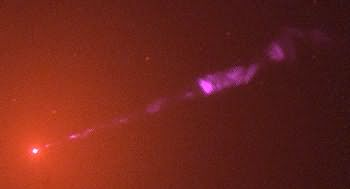
\includegraphics[max width=\linewidth]{../images/m87_jet.jpg}}\]

\begin{enumerate}
\def\labelenumi{\arabic{enumi})}
\tightlist
\item
  NASA and John Biretta, ``M87'',
  \texttt{http://hubblesite.org/newscenter/newsdesk/archive/releases/2005/12/image/o}
\end{enumerate}

M87 is a giant elliptical galaxy. It's long been known as a powerful
radio source, and now we know why: there's a supermassive black hole in
the center, about 3 billion times the mass of our Sun. As matter spirals
into this huge black hole, it forms an ``accretion disk'', and some gets
so hot that it shoots out in a jet, as envisioned here:
\[\href{http://maxim.gsfc.nasa.gov/docs/science/science.html}{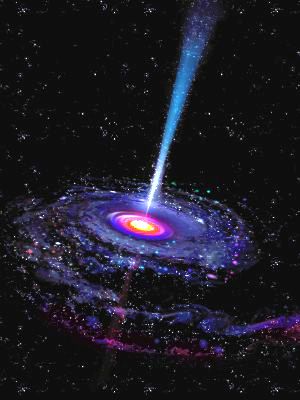
\includegraphics[max width=\linewidth]{../images/accretion_disk.jpg}}\]

\begin{enumerate}
\def\labelenumi{\arabic{enumi})}
\setcounter{enumi}{1}
\tightlist
\item
  NASA, MAXIM: ``Micro-Arcsecond X-ray Imaging Mission'',
  \texttt{http://maxim.gsfc.nasa.gov/docs/science/science.html}
\end{enumerate}

Accretion disks and jets are common at many different scales in our
universe. They're just nature's way of letting a bunch of matter fall in
under its own gravitation while losing angular momentum and energy. We
see them when dust clouds collapse to form stars, we see them when black
holes sucks in mass from companion stars, and they're probably also
responsible for slow \(\gamma\) ray bursts as huge stars collapse when
they run out of fuel --- see \protect\hyperlink{week204}{``Week 204''}
for that story.

But, among the biggest accretion disks and jets are those surrounding
supermassive black holes in the middle of galaxies. These are probably
responsible for all the ``active galactic nuclei'' or ``quasars'' that
we see. In the case of M87 the jet is enormous: 5000 light years long!
To get a sense of the scale, look at the small white specks away from
the jet in the next picture. These are globular clusters: clusters
containing between ten thousand and a million stars.
\[\href{http://antwrp.gsfc.nasa.gov/apod/ap000706.html}{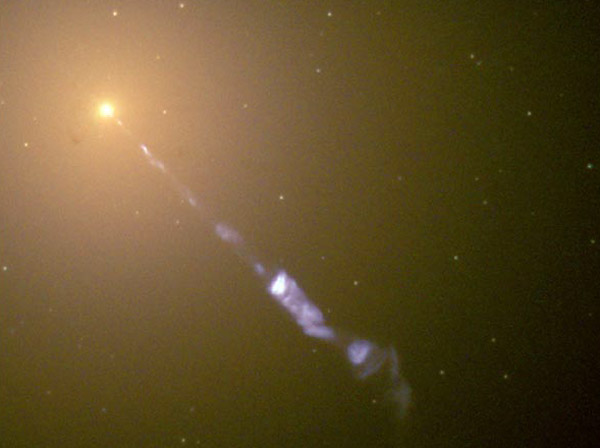
\includegraphics[max width=\linewidth]{../images/m87jet_hst.jpg}}\]

\begin{enumerate}
\def\labelenumi{\arabic{enumi})}
\setcounter{enumi}{2}
\tightlist
\item
  A jet from galaxy M87, ``Astronomy Picture of the Day, July 6, 2000'',
  \texttt{http://antwrp.gsfc.nasa.gov/apod/ap000706.html}
\end{enumerate}

The jet in M87 is so hot that it emits not just radio waves and visible
light, but even X-rays, as seen by the Chandra X-ray telescope:
\[\href{http://chandra.harvard.edu/photo/2001/0134/}{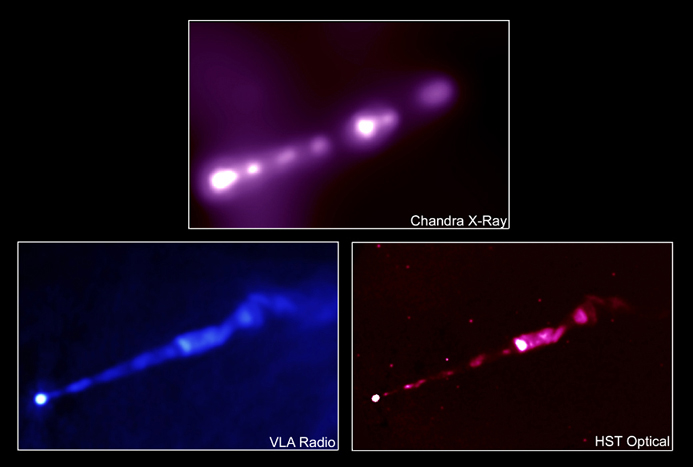
\includegraphics[max width=\linewidth]{../images/m87_xray_radio_optical.jpg}}\]

\begin{enumerate}
\def\labelenumi{\arabic{enumi})}
\setcounter{enumi}{3}
\tightlist
\item
  ``M87: Chandra sheds light on the knotty problem of the M87 jet'',
  \texttt{http://chandra.harvard.edu/photo/2001/0134/}
\end{enumerate}

It seems the jet consists mainly of electrons moving at relativistic
speeds, focused by the magnetic field of the accretion disk. They come
in blobs called ``knots''. People can actually see these blobs moving
out, getting brighter and dimmer.

In fact, many galaxies have super-massive black holes at their centers
with jets like this one. The special thing about M87 is that it's fairly
nearby, hence easy to see. M87 is the biggest galaxy in the Virgo
Cluster. This is the closest galaxy cluster to us, about 50 million
light years away. That sounds pretty far, but it's only 1000 times the
radius of the Milky Way. If the Milky Way were a pebble, M87 would be
only a stone's throw away. So, even amateur astronomers --- really good
ones, at least --- can take photos of M87 that show the jet. But here's
a high-quality picture produced by Robert Lupton using data from the
Sloan Digital Sky Survey --- you can see the jet in light blue:
\[\href{http://www.astro.princeton.edu/~rhl/PrettyPictures/}{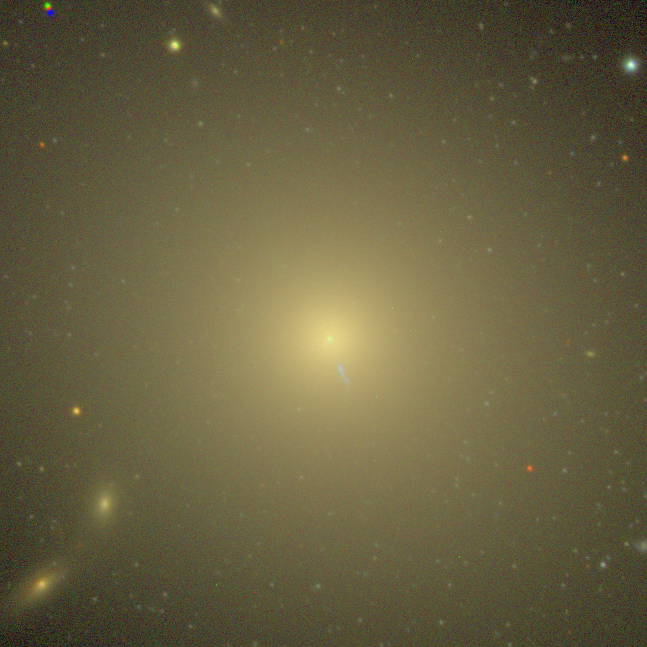
\includegraphics[max width=\linewidth]{../images/m87_core.jpg}}\]

\begin{enumerate}
\def\labelenumi{\arabic{enumi})}
\setcounter{enumi}{4}
\tightlist
\item
  Robert Lupton and the Sloan Digital Sky Survey Consortium, ``The
  central regions of M87'',
  \texttt{http://www.astro.princeton.edu/\textasciitilde{}rhl/PrettyPictures/}
\end{enumerate}

Backing off a bit further, let's take a look at the Virgo Cluster. It
contains over a thousand galaxies, but we can tell it's fairly new as
clusters go, since it consists of a bunch of ``subclusters'' that
haven't merged yet. Our galaxy, and indeed the whole Local Group to
which it belongs, is being pulled towards the Virgo Cluster and will
eventually join it. Here's a nice closeup of part of the Virgo Cluster:
\[\href{http://burro.astr.cwru.edu/Schmidt/Virgo/}{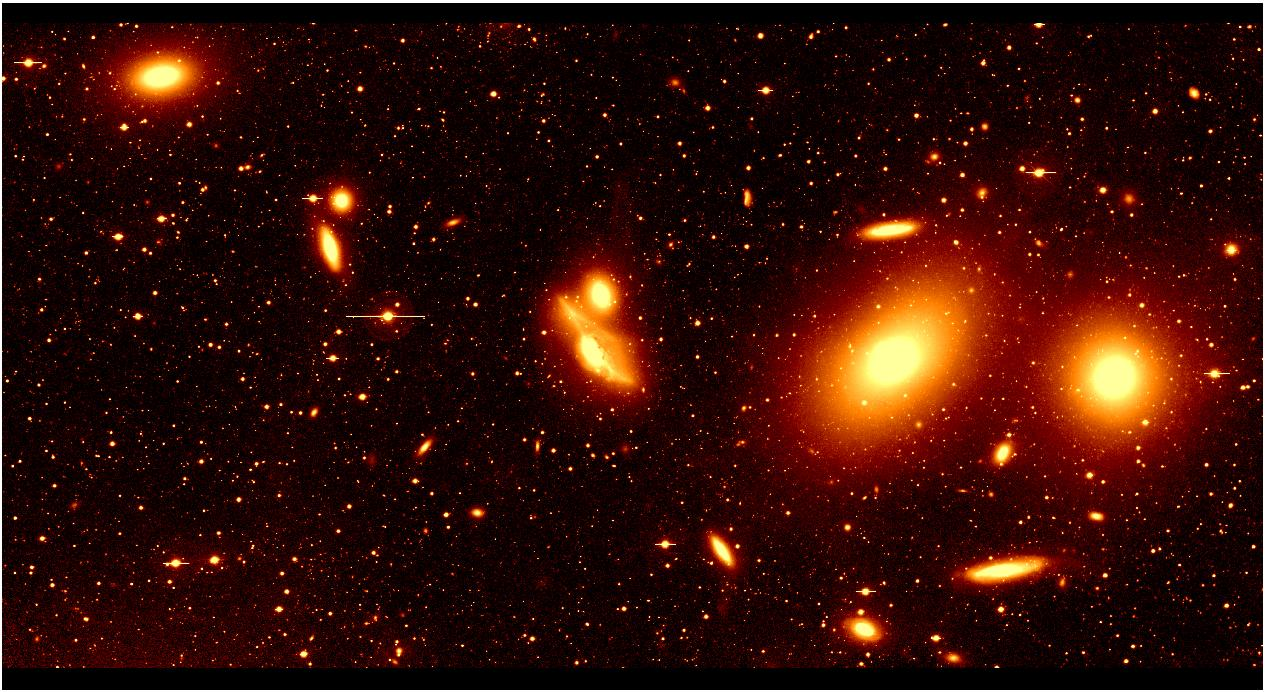
\includegraphics[max width=\linewidth]{../images/virgo_cluster.jpg}}\]

\begin{enumerate}
\def\labelenumi{\arabic{enumi})}
\setcounter{enumi}{5}
\tightlist
\item
  Chris Mihos, Paul Harding, John Feldmeier and Heather Morrison, ``Deep
  imaging of the Virgo Cluster'',
  \texttt{http://burro.astr.cwru.edu/Schmidt/Virgo/}
\end{enumerate}

Finally, just for fun, something unrelated --- and more mysterious. It's
called ``Hoag's object'':
\[\href{http://heritage.stsci.edu/2002/21/}{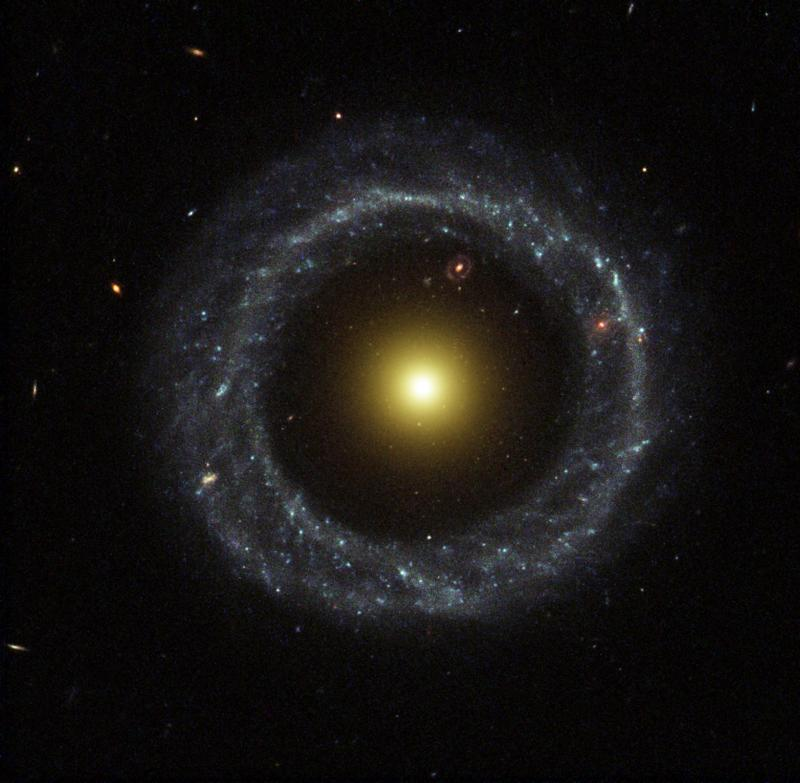
\includegraphics[max width=\linewidth]{../images/hoag.jpg}}\]

\begin{enumerate}
\def\labelenumi{\arabic{enumi})}
\setcounter{enumi}{6}
\tightlist
\item
  The Hubble Heritage Project, ``Hoag's Object'',
  \texttt{http://heritage.stsci.edu/2002/21/}
\end{enumerate}

It's a ring-shaped galaxy full of hot young blue stars surrounding a
ball of yellower stars. Nobody knows how it formed: perhaps by a
collision of two galaxies? Such collisions are fairly common, but they
don't typically create this sort of structure.

The weirdest part is that inside the ring, in the upper right, you can
see \emph{another} ring galaxy in the distance! Maybe an advanced
civilization over there enjoys this form of art? Probably not, but if it
turns out to be true, you heard it here first.

Anyway\ldots{} back here on Earth, in the summer of 2004, I visited
Dublin for a conference on general relativity called GR17. As recounted
in \protect\hyperlink{week207}{``Week 207''}, this was where Hawking
admitted defeat in his famous bet with John Preskill about information
loss due to black hole evaporation. In August of this year, Hawking
finally came out with a short paper on the subject:

\begin{enumerate}
\def\labelenumi{\arabic{enumi})}
\setcounter{enumi}{7}
\tightlist
\item
  Stephen W. Hawking, ``Information loss in black holes'', available as
  \href{https://arxiv.org/abs/hep-th/0507171}{\texttt{hep-th/0507171}}.
\end{enumerate}

I spent a lot of time talking to physicists, but I also wandered around
Dublin a bit. Besides listening to some great music at a pub called
Cobblestones --- Kevin Rowsome plays a mean uilleann pipe! --- and
tracking down some sites mentioned in James Joyce's novel ``Ulysses'', I
went with Tevian Dray on a pilgrimage to Brougham Bridge.

Tevian Dray is an expert on the octonions, and Brougham Bridge is where
Hamilton carved his famous formula defining the quaternions! Now there
is a plaque commemorating this event, which reads:

\begin{quote}
Here as he walked by\\
on the 16th of October 1843\\
Sir William Rowan Hamilton\\
in a flash of genius discovered\\
the fundamental formula for\\
quaternion multiplication\\
\(i^2 = j^2 = k^2 = ijk = -1\)\\
\& cut it on a stone of this bridge
\end{quote}

It does't mention that Hamilton had been racking his brain for the
entire month of October trying to solve this problem: ``flashes of
genius'' favor the prepared mind. But it's a nice story and a nice
place. My friend Tevian Dray took some photos, which you can see here:

\begin{enumerate}
\def\labelenumi{\arabic{enumi})}
\setcounter{enumi}{8}
\tightlist
\item
  John Baez, ``Dublin'', \texttt{http://math.ucr.edu/home/baez/dublin/}
\end{enumerate}

It was a bit of a challenge finding Brougham Bridge, since nobody at the
main bus station gave us correct information about which bus went there
--- except the bus driver who finally took us there. So, to ease your
way in case you want to make your own pilgrimage, the above page
includes directions. And now, thanks to Dirk Schlimm, it also includes a
link to a map showing the bridge!

Speaking of Hamilton, Theron Stanford recently sent me an answer to one
of life's persistent questions: why is momentum denoted by the letter p?

Since momentum and position play fundamental roles in Hamiltonian
mechanics, and they're denoted by \(p\) and \(q\), one wonders: could
this notation be related to Hamilton's alcoholism in later life? After
all, some claim the saying \emph{mind your p's and q's} began as a
friendly Irish warning not to imbibe too many pints and quarts! So,
maybe he used these letters in his work on physics as a secret plea for
help.

Umm\ldots{} probably not. Just kidding. But in the absence of hard
facts, speculation runs rampant. So, I'm glad Stanford provided some of
the former, to squelch the latter.

He sent me this email:

\begin{quote}
While Googling various subjects, I came across
\href{http://math.ucr.edu/home/baez/qg-winter2001/qg12.2.html}{the
following} from your
\href{http://math.ucr.edu/home/baez/QG.html}{Quantum Gravity Seminar}
notes from 2001:

\begin{quote}
Again Oz was overcome with curiosity, so mimicking Toby's voice, he
asked, ``Why do we call the momentum \(p\)?''

The Wiz glared at Toby. ``Because \(m\) is already taken -- it stands
for mass! Seriously, I don't know why people call position \(q\) and
momentum \(p\). All I know is that if you use any other letters, people
can tell you're not a physicist. So I urge you to follow tradition on
this point.''
\end{quote}

Well, I have an answer. Hamilton, the first physicist to actually
understand the importance of the concept of momentum, chose \(\varpi\)
to stand for momentum (it's not the usual \(\pi\), but what TeX calls
\texttt{varpi}, a lower-case \(\omega\) with a top, kinda like the top
of a lower-case \(\tau\)). Jacobi changed this to \(p\) in one of his
seminal papers on the subject; he also used \(q\) in the same paper to
stand for position. In the 1800s (I want to say 1850s, though it might
have been a decade or two later) Cayley presented a paper to the Royal
Academy in which he says (and I paraphrase), ``Well, it seems that \(p\)
and \(q\) are pretty well established now, so that's what I'm going to
use.''
\end{quote}

So, now the question is why Hamilton chose the letter \(\varpi\) for
momentum. This variant of \(\pi\) was fairly common in the mathematical
literature of the day, so there may be no special explanation. For some
further detective work, see:

\begin{enumerate}
\def\labelenumi{\arabic{enumi})}
\setcounter{enumi}{9}
\tightlist
\item
  ``Hamilton: two mysteries solved'',
  \texttt{http://groups.google.com/group/sci.physics/browse\_thread/thread/d1b7b4a998682bbb/3a868ae8218a4bca\#3a868ae8218a4bca}
\end{enumerate}

Also see equation 12 in this paper for one of the first uses of
``\(\varpi\)'' to mean momentum:

\begin{enumerate}
\def\labelenumi{\arabic{enumi})}
\setcounter{enumi}{10}
\tightlist
\item
  William Rowan Hamilton, ``Second essay on a general method in
  dynamics'', ed.~David R. Wilkins, available at
  \texttt{http://www.maths.tcd.ie/pub/HistMath/People/Hamilton/Dynamics/SecEssay.pdf}
\end{enumerate}

He doesn't say why he chose this letter --- it may have been completely
random!

Before I turn to higher-dimensional algebra, maybe this is a good time
to mention a paper related to the octonions:

\begin{enumerate}
\def\labelenumi{\arabic{enumi})}
\setcounter{enumi}{11}
\tightlist
\item
  Jakob Palmkvist, ``A realization of the Lie algebra associated to a
  Kantor triple system'', available as
  \href{http://arxiv.org/abs/math.RA/0504544}{\texttt{math.RA/0504544}}.
\end{enumerate}

In \protect\hyperlink{week193}{``Week 193''} I mentioned how
\(3\)-graded Lie algebras come from ``Jordan triple systems'', and
vaguely hinted that \(5\)-graded Lie algebras come from ``Kantor triple
systems''. I explained how the exceptional Lie algebra \(\mathrm{E}_8\)
gets to be \(5\)-graded, but I didn't really say anything about Kantor
triple systems because my understanding of them was so poor. This paper
by Palmkvist explains them very clearly! And even better, he shows how
the ``magic square'' Lie algebras \(\mathrm{F}_4\), \(\mathrm{E}_6\),
\(\mathrm{E}_7\), and \(\mathrm{E}_8\) can be systematically obtained
from the octonions, bioctonions, quateroctonions and octooctonions by
means of Kantor triple systems.

Now for some mathematical physics that touches on higher-dimensional
algebra. If you still don't get why topological field theory and
\(n\)-categories are so cool, read this thesis:

\begin{enumerate}
\def\labelenumi{\arabic{enumi})}
\setcounter{enumi}{12}
\tightlist
\item
  Bruce H. Bartlett, \emph{Categorical aspects of topological quantum
  field theories}, M.Sc. Thesis, Utrecht University, 2005. Available as
  \href{http://arxiv.org/abs/math.QA/0512103}{\texttt{math.QA/0512103}}.
\end{enumerate}

It's a great explanation of the big picture! I can't wait to see what
Bartlett does for his Ph.D..

If you're a bit deeper into this stuff, you'll enjoy this:

\begin{enumerate}
\def\labelenumi{\arabic{enumi})}
\setcounter{enumi}{13}
\tightlist
\item
  Aaron Lauda and Hendryk Pfeiffer, ``Open-closed strings:
  two-dimensional extended TQFTs and Frobenius algebras'', available as
  \href{http://arxiv.org/abs/math.AT/0510664}{\texttt{math.AT/0510664}}.
\end{enumerate}

This paper gives a purely algebraic description of the topology of open
and closed strings, making precise and proving some famous results
stated without proof by Moore and Segal, which can be seen here:

\begin{enumerate}
\def\labelenumi{\arabic{enumi})}
\setcounter{enumi}{14}
\tightlist
\item
  Greg Moore, ``Lectures on branes, K-theory and RR charges'',
  \emph{Clay Math Institute Lecture Notes} (2002), available at
  \texttt{http://www.physics.rutgers.edu/\textasciitilde{}gmoore/clay1/clay1.html}
\end{enumerate}

Lauda and Pfeiffer's paper makes heavy use of Frobenius algebras,
developing more deeply some of the themes I mentioned in
\protect\hyperlink{week174}{``Week 174''}. In a related piece of work,
Lauda has figured out how to \emph{categorify} the concept of a
Frobenius algebra, and has applied this to 3d topology:

\begin{enumerate}
\def\labelenumi{\arabic{enumi})}
\setcounter{enumi}{15}
\item
  Aaron Lauda, ``Frobenius algebras and ambidextrous adjunctions'',
  \href{http://www.tac.mta.ca/tac/volumes/16/4/16-04abs.html}{\emph{Theory
  and Applications of Categories} \textbf{16} (2006) 84--122}. Also
  available as
  \href{http://arxiv.org/abs/math.CT/0502550}{\texttt{math.CT/0502550}}.

  Aaron Lauda, ``Frobenius algebras and planar open string topological
  field theories'', available as
  \href{http://arxiv.org/abs/math.QA/0508349}{\texttt{math.QA/0508349}}.
\end{enumerate}

The basic idea behind all this work is a ``periodic table'' of
categorified Frobenius algebras, which are related to topology in
different dimensions. For example, in \protect\hyperlink{week174}{``Week
174''} I explained how Frobenius algebras formalize the idea of paint
drips on a sheet of rubber. As you move your gaze down a sheet of rubber
covered with drips of paint, you'll notice that drips can merge:

\begin{verbatim}
                      \ \         / /  
                       \ \       / /
                        \ \     / /
                         \ \   / /
                          \ \_/ /      
                           \   /                                        
                            | |
                            | |
                            | |
                            | |
                            | |   
\end{verbatim}

but also split:

\begin{verbatim}
                            | |
                            | |   
                            | |
                            | |
                            | |
                           / _ \                                            
                          / / \ \      
                         / /   \ \
                        / /     \ \
                       / /       \ \
                      / /         \ \ 
\end{verbatim}

In addition, drips can start:

\begin{verbatim}
                            _
                           | |
                           | |
                           | |
                           | |
                           | |
                           | |
                           | |
                           | |
                           | |
\end{verbatim}

but also end:

\begin{verbatim}
                           | |
                           | |
                           | |
                           | |
                           | |
                           | |
                           | |
                           | |
                           |_|
\end{verbatim}

In a Frobenius algebra, these four pictures correspond to four
operations called ``multiplication'' (merging), ``comultiplication''
(splitting), the ``unit'' (starting) and the ``counit'' (ending).
Moreover, these operations satisfy precisely the relations that you can
prove by warping the piece of rubber and seeing how the pictures change.
For example, there's the associative law:

\begin{verbatim}
            \ \    / /    / /      \ \    \ \    / /
             \ \  / /    / /        \ \    \ \  / /
              \ \/ /    / /          \ \    \ \/ /
               \  /    / /            \ \    \  /
                \ \   / /              \ \   / /
                 \ \_/ /                \ \_/ /
                  \   /                  \   /
                   | |                    | |
                   | |                    | |    
                   | |          =         | |
                   | |                    | |
                   | |                    | |
                   | |                    | |
                   | |                    | |
                   | |                    | |
\end{verbatim}

The idea here is that if you draw the picture on the left-hand side on a
sheet of rubber, you can warp the rubber until it looks like the
right-hand side! There's also the ``coassociative law'', which is just
an upside-down version of the above picture. But the most interesting
laws are the ``\(I = N\)'' equation:

\begin{verbatim}
               \ \     / /                | |        | |
                \ \   / /                 | |        | |
                 \ \_/ /                  | |        | |
                  \   /                   |  \       | |
                   | |                    |   \      | |
                   | |                    | |\ \     | |   
                   | |                    | | \ \    | |
                   | |                    | |  \ \   | |
                   | |          =         | |   \ \  | |
                   | |                    | |    \ \ | |
                   | |                    | |     \ | |
                   | |                    | |      \   |
                  / _ \                   | |       \  |
                 / / \ \                  | |        | |
                / /   \ \                 | |        | | 
               / /     \ \                | |        | |
\end{verbatim}

and its mirror-image version.

So, the concept of Frobenius algebra captures the topology of regions in
the plane! Aaron Lauda makes this fact into a precise theorem in his
paper on planar open string field theories, and then generalizes it to
consider ``categorified'' Frobenius algebras where the above equations
are replaced by isomorphisms, which describe the \emph{process} of
warping the sheet of rubber until the left side looks like the right.
You should look at his paper even if you don't understand the math,
because it's full of cool pictures.

Lauda and Pfeiffer's paper goes still further, by considering these
paint stripes as ``open strings'', not living in the plane anymore, but
zipping around in some spacetime of high dimension, where they might as
well be abstract 2-manifolds with corners. Following Moore and Segal,
they also bring ``closed strings'' into the game, which form a Frobenius
algebra of their own, where the multiplication looks like an upside-down
pair of pants: \[
  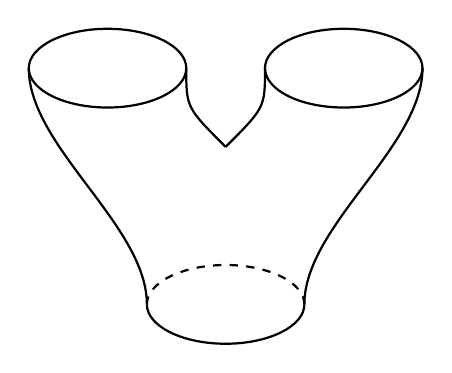
\begin{tikzpicture}[scale=0.5]
    \draw[thick] (-3,0) ellipse (2cm and 1cm);
    \draw[thick] (3,0) ellipse (2cm and 1cm);
    \draw[thick] (-5,0) .. controls (-5,-2) and (-2,-4) .. (-2,-6);
    \draw[thick] (5,0) .. controls (5,-2) and (2,-4) .. (2,-6);
    \draw[thick] (-1,0) .. controls (-1,-1) .. (0,-2);
    \draw[thick] (1,0) .. controls (1,-1) .. (0,-2);
    \begin{scope}[shift={(0,-6)}]
      \draw[thick,dashed] (0:2) arc (0:180:2cm and 1cm);
      \draw[thick] (180:2) arc (180:360:2cm and 1cm);
    \end{scope}
  \end{tikzpicture}
\] These topological closed strings are the subject of Joachim Kock's
book mentioned in \protect\hyperlink{week202}{``Week 202''}; they
correspond to \emph{commutative} Frobenius algebras. The fun new stuff
comes from letting the open strings and closed strings interact.

You can read more about Lauda and Pfeiffer's work at Urs Schreiber's
blog:

\begin{enumerate}
\def\labelenumi{\arabic{enumi})}
\setcounter{enumi}{16}
\tightlist
\item
  Urs Schreiber, ``Lauda and Pfeiffer on open-closed topological
  strings'',
  \texttt{http://golem.ph.utexas.edu/string/archives/000680.html}
\end{enumerate}

In fact, I recommend Schreiber's blog quite generally to anyone
interested in higher categories and/or the math of string theory!

\begin{center}\rule{0.5\linewidth}{0.5pt}\end{center}

\textbf{Addendum:} Bruce Smith, David Rusin and Robert Lupton had some
comments about the astronomy section; Urs Schreiber had more to say
about the role of Frobenius algebras in string theory.

Bruce Smith picked up on my comment about accretion disks being common
at many different scales, and wondered what the smallest accretion disks
are. We talked about it and agreed that hurricanes, tornados, dust
devils and whirlpools are \emph{related} phenomena, but not true
accretion disks.

Given this, the smallest accretion disks I know are those that led to
the formation of planets in our Solar System, and perhaps even some
moons. These probably began as eddies in the bigger accretion disk that
became our Sun. The Sun is about 300,00 times heavier than the Earth,
and the super-massive black hole in M87 is about 3 billion times heavier
than the Sun, so we're seeing accretion disks that differ in mass by a
factor of a trillion!

David Rusin's reaction to Hoag's object was:

\begin{quote}
Cool. But what are the chances that there would be not just one but TWO
fascinating objects which have a significant plane of symmetry, which
``just happens'' to be perpendicular to our line of sight?
\end{quote}

He asked how many ring galaxies are known!

I checked and read there are 100 known ``polar-ring galaxies''. Here's a
nice one called NGC 4650:
\[\href{http://hubblesite.org/newscenter/newsdesk/archive/releases/1999/16/image/a}{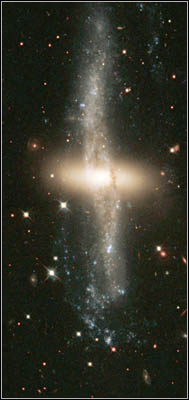
\includegraphics[max width=\linewidth]{../images/NGC4650.jpg}}\]

\begin{enumerate}
\def\labelenumi{\arabic{enumi})}
\setcounter{enumi}{17}
\tightlist
\item
  ``Ring around a galaxy'', \emph{HubbleSite News Archive}, May 6, 1999,
  \texttt{http://hubblesite.org/newscenter/newsdesk/archive/releases/1999/16/image/a}
\end{enumerate}

I can imagine this thing looking like Hoag's object if we viewed it
head-on.

Here's another ring galaxy, called AM 0644-741:
\[\href{http://hubblesite.org/newscenter/newsdesk/archive/releases/2004/15/image/a}{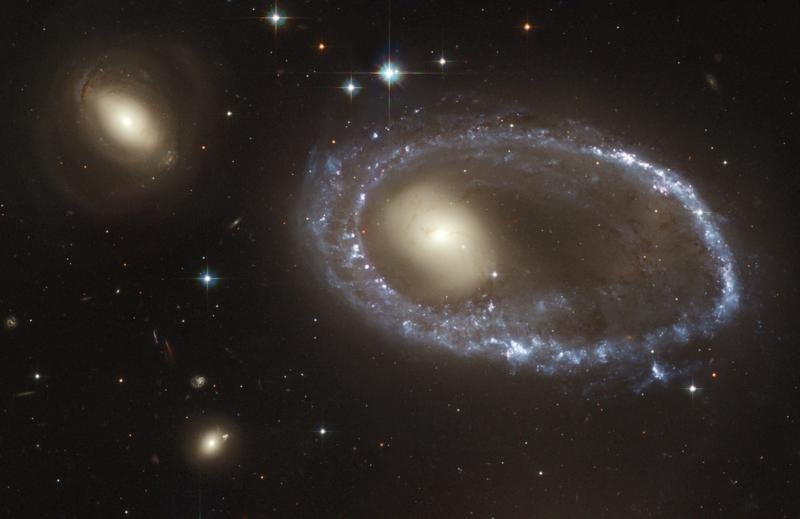
\includegraphics[max width=\linewidth]{../images/AM0644-741.jpg}}\]

\begin{enumerate}
\def\labelenumi{\arabic{enumi})}
\setcounter{enumi}{18}
\tightlist
\item
  ``The lure of the rings'', \emph{Hubblesite News Archive}, April 22,
  2004,
  \texttt{http://hubblesite.org/newscenter/newsdesk/archive/releases/2004/15/image/a}
\end{enumerate}

It's the result of a collision involving a galaxy that's not in this
picture. So, maybe Hoag's object is just a specially pretty case of a
galaxy collision!

Robert Lupton referred me to a picture that covers more of the Virgo
Cluster --- but the file is huge, so I won't include it here:

\begin{enumerate}
\def\labelenumi{\arabic{enumi})}
\setcounter{enumi}{19}
\tightlist
\item
  Doug Finkbeiner and the Sloan Digital Sky Survey Consortium, ``Some
  pretty objects as observed by the SDSS: Virgo Cluster'',
  \texttt{http://www.astro.princeton.edu/\textasciitilde{}rhl/dfink}
\end{enumerate}

See the lower right corner for the picture called ``virgobig''.

Here's what Urs Schreiber had to say about Frobenius algebras and string
theory:

\begin{quote}
John Baez wrote:

\begin{quote}
{[}\ldots{]} Following Moore and Segal, they also bring ``closed
strings'' into the game, which form a Frobenius algebra of their own,
where the multiplication looks like an upside-down pair of pants:
{[}\ldots{]}
\end{quote}

I would like to make the following general comment on the meaning of
Frobenius algebras in \(2\)-dimensional quantum field theory.

Interestingly, \emph{non}-commutative Frobenius algebras play a role
even for closed strings, and even if the worldhseet theory is not purely
topological.

The archetypical example for this is the class of 2D TFTs invented by
Fukuma, Hosono and Kawai. There one has a non-commutative Frobenius
algebra which describes not the splitting/joining of the entire
worldsheet, but rather the splitting/joining of edges in any one of its
dual triangulations. It is the \emph{center} of (the Morita class of)
the noncommutative Frobenius algebra decorating dual triangulations
which is the commutative Frobenius algebra describing the closed 2D TFT.

One might wonder if it has any value to remember a non-commutative
Frobenius algebra when only its center matters (in the closed case). The
point is that the details of the non-commutative Frobenius algebra
acting in the ``interior'' of the world sheet affects the nature of
``bulk field insertions'' that one can consider and hence affects the
(available notions of) \(n\)-point correlators of the theory, for
\(n > 0\).

This aspect, however, is pronounced only when one switches from 2D
topological field theories to conformal ones.

The fascinating thing is that even 2D \emph{conformal} field theories
are governed by Frobenius algebras. The difference lies in different
categorical internalization. The Frobenius algebras relevant for CFT
don't live in \(\mathsf{Vect}\), but in some other (modular) tensor
category, usually that of representations of some chiral vertex operator
algebra. It is that ambient tensor category which ``knows'' if the
Frobenius algebra describes a topological or a conformal field theory
(in 2D) --- and which one.

Of course what I am referring to here is the work by Fjelstad,
Froehlich, Fuchs, Runkel, Schweigert and others. I can recommend their
most recent review which will appear in the Streetfest proceedings. It
is available as
\href{http://arxiv.org/abs/math.CT/0512076}{\texttt{math.CT/0512076}}.

The main result is, roughly, that given any modular tensor category with
certain properties, and given any (symmetric and special) Frobenius
algebra object internal to that category, one can construct functions on
surfaces that satisfy all the properties that one would demand of an
\(n\)-point function of a 2D (conformal) field theory.

If we define a field theory to be something not given by an ill-defined
path integral, but something given by its set of correlation functions,
then this amounts to constructing a (conformal) field theory.

This result is achieved by first defining a somewhat involved procedure
for generating certain classes of functions on marked surfaces, and then
proving that the functions generated by this procedure do indeed satisfy
all the required properties.

In broad terms, the prescription is to choose a dual triangulation of
the marked worldsheet whose correlation function is to be computed, to
decorate its edges with symmetric special Frobenius algebra objects in
some modular tensor category, to decorate its vertices by product and
coproduct morphisms of this algebra, to embed the whole thing in a
certain \(3\)-manifold in a certain way and for every boundary or bulk
field insertion to add one or two threads labeled by simple objects of
the tensor category which connect edges of the chosen triangulation with
the boundary of that \(3\)-manifold. Then you are to hit the resulting
extended \(3\)-manifold with the functor of a 3D TFT and hence obtain a
vector in a certain vector space. This vector, finally, is claimed to
encode the correlation function.

This procedure is deeply rooted in well-known relations between
\(3\)-(!)-dimensional topological field theory, modular functors and
modular tensor categories and may seem very natural to people who have
thought long enough about it. It is already indicated in Witten's paper
on the Jone's polynomial, that 3D TFT (Chern-Simons field theory in that
case) computes conformal blocks of conformal field theories on the
boundaries of these \(3\)-manifolds. To others, like me in the
beginning, it may seem like a miracle that an involved and superficially
ad hoc procedure like this has anything to do with correlations
functions of conformal field theory in the end.

In trying to understand the deeper ``meaning'' of it all I played around
with the idea that this prescription is really, to some extent at least,
the ``dual'' incarnation of the application of a certain \(2\)-functor
to the worldsheet. Namely a good part of the rough structure appearing
here automatically drops out when a \(2\)-functor applied to some
\(2\)-category of surfaces is ``locally trivialized''. I claim that any
local trivialization of a \(2\)-functor on some sort of \(2\)-category
of surface elements gives rise to a dual triangulation of the surface
whose edges are labeled by (possibly a generalization of) a Frobenius
algebra object and whose vertices are labeled by (possibly a
generalization of) product and coproduct operations. There is more data
in a locally trivialized \(2\)-functor, and it seems to correctly
reproduce the main structure of bulk field insertions as appearing
above. But of course there is a limit to what a \emph{2}-functor can
know about a structure that is inherently \(3\)-dimensional.

I have begun outlining some of the details that I have in mind here:

\texttt{http://golem.ph.utexas.edu/string/archives/000697.html}

This has grown out of a description of gerbes with connective structure
in terms of transport \(2\)-functors. Note that in what is called a
\emph{bundle} gerbe we also do have a certain product operation playing
a decisive role. Bundle gerbes can be understood as
``pre-trivializations'' of \(2\)-functors to \(\mathsf{Vect}\):

\texttt{http://golem.ph.utexas.edu/string/archives/000686.html}

and the product appearing is one of the Frobenius products mentioned
above. For a bundle gerbe the coproduct is simply the inverse of the
product, since this happens to be an isomorphism. The claim is that
\(2\)-functors to \(\mathsf{Vect}\) more generally give rise to
non-trivial Frobenius algebras when locally trivialized.

This is work in progress and will need to be refined. I thought I'd
mention it here as a comment to John's general statements about how
Frobenius algebras know about \(2\)-dimensional physics. I am grateful
for all kinds of comments.
\end{quote}

Here's the paper Urs refers to:

\begin{enumerate}
\def\labelenumi{\arabic{enumi})}
\setcounter{enumi}{20}
\tightlist
\item
  Ingo Runkel, Jens Fjelstad, Jurgen Fuchs and Christoph Schweigert,
  ``Topological and conformal field theory as Frobenius algebras'',
  available as
  \href{http://arxiv.org/abs/math.CT/0512076}{\texttt{math.CT/0512076}}.
\end{enumerate}

\begin{center}\rule{0.5\linewidth}{0.5pt}\end{center}

\begin{quote}
\emph{Here's how you do it:\\
First you're obtuse,\\
Then you intuit,\\
Then you deduce!}

--- Garrison Keillor
\end{quote}



\hypertarget{week225}{%
\section{December 24, 2005}\label{week225}}

Happy holidays! I'll start with some gift suggestions for people who put
off their Christmas shopping a bit too long, before moving on to this
week's astronomy pictures and then some mathematical physics: minimal
surfaces.

Back in 2000 I listed some gift ideas in
\protect\hyperlink{week162}{``Week 162''}. I decided to do it again this
year. After all, where else can you read about quantum gravity,
nonabelian cohomology, higher categories\ldots{} and also get helpful
shopping tips? But, I put off writing this Week's Finds a bit too late.
Oh well.

I just saw this book in a local store, and it's \emph{great}:

\begin{enumerate}
\def\labelenumi{\arabic{enumi})}
\tightlist
\item
  Robert Dinwiddie, Philip Eales, David Hughes, Ian Nicholson, Ian
  Ridpath, Giles Sparrow, Pam Spence, Carole Stott, Kevin Tildsley, and
  Martin Rees, \emph{Universe}, DK Publishing, New York, 2005.
\end{enumerate}

If you like the astronomy pictures you've seen here lately, you'll love
this book, because it's \emph{full} of them --- all as part of a
well-organized, clearly written, information-packed but nontechnical
introduction to astronomy. It starts with the Solar System and sails out
through the Oort Cloud to the Milky Way to the Local Group to the Virgo
Supercluster \ldots{} and all the way out and back to the Big Bang!

The only thing this book seems to lack --- though I could have missed it
--- is a 3d map showing the relative scales of our Solar System, Galaxy,
and so on. I recommended a wall chart like this back in
\protect\hyperlink{week162}{``Week 162''}, and my friend Danny Stevenson
just bought me one. I'll probably put it up near my office in the math
department\ldots{} gotta keep the kids thinking big!

You don't really need to buy a chart like this. You can just look at
this website:

\begin{enumerate}
\def\labelenumi{\arabic{enumi})}
\setcounter{enumi}{1}
\tightlist
\item
  Richard Powell, ``An Atlas of the Universe'',
  \texttt{http://www.anzwers.org/free/universe/}
\end{enumerate}

It has nine maps, starting with the stars within 12.5 light years and
zooming out repeatedly by factors of 10 until it reaches the limits of
the observable universe, roughly 14 billion light years away. Or more
precisely, 14 billion years ago!

(The farther we look, the older things we see, since light takes time to
travel. The most distant thing we see is light released when hot gas
from the Big Bang cooled down just enough to let light through! If we
calculate how far this gas would be \emph{now}, thanks to the expansion
of the universe, we get a figure of roughly 78 billion light years. But
of course we can't see what that gas looks like \emph{now} unless we
wait a lot longer. It's a bit confusing until you think about it for a
while.)

For example, here are the clusters of galaxies within 100 million
lightyears of us:
\[\href{http://www.anzwers.org/free/universe/virgo.html}{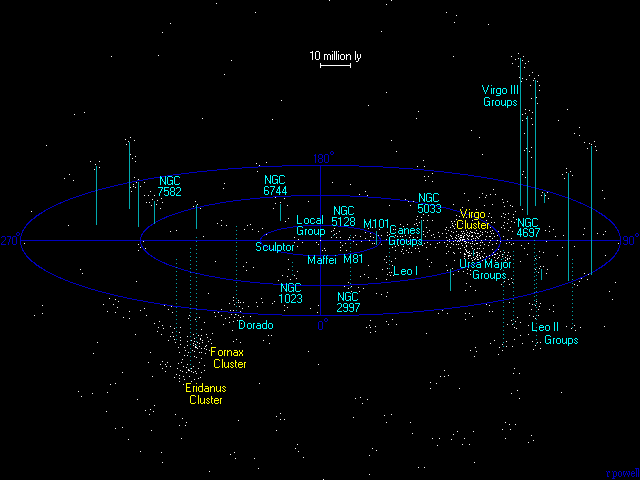
\includegraphics[max width=\linewidth]{../images/Virgo_supercluster.png}}\]

The biggest of these is the Virgo cluster, which I discussed in
\protect\hyperlink{week224}{``Week 224''}. This contains about 2000
galaxies. The second biggest is the Fornax cluster. The whole
agglomeration shown here is called the Virgo Supercluster. Superclusters
are among the biggest structures in the universe.

This atlas is fun to browse when you're at your computer. But, if
someone you know wants to contemplate the universe in a more relaxing
way, try getting them one of these:

\begin{enumerate}
\def\labelenumi{\arabic{enumi})}
\setcounter{enumi}{2}
\item
  Bathsheba Grossman, ``Crystal model of a typical 100-megaparsec cube
  of the universe'',
  \texttt{http://www.bathsheba.com/crystal/largescale/}

  ``Crystal model of the Milky Way'',
  \texttt{http://www.bathsheba.com/crystal/galaxy/}
\end{enumerate}

I found out about these from David Scharffenberg, who owns the Riverside
Computer Center nearby --- a cool little shop that's decorated with
archaic technology ranging from a mammoth slide rule to a gizmo that
computes square roots using air pressure. He gave me the 100-megaparsec
cube as a present, and it's great! It's lit up from below, and it shows
the filaments, sheets and superclusters of galaxies that reign supreme
at this distance scale. 100 megaparsecs is about 300 million light
years, so this view is a bit bigger than the previous picture:
\[\href{http://www.bathsheba.com/crystal/largescale/}{\includegraphics[max width=\linewidth]{../images/largescale_movie2.png}}\]

David says Grossman's model of the Milky Way is also nice: it takes into
account the latest research, which shows our galaxy is a ``barred''
spiral! You can see the bar in the middle here:
\[\href{http://www.spitzer.caltech.edu/Media/mediaimages/sig/sig05-010.shtml}{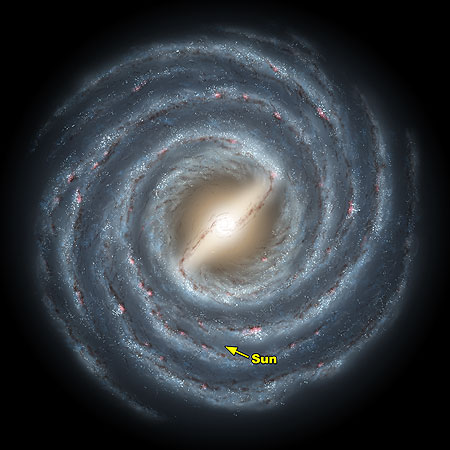
\includegraphics[max width=\linewidth]{../images/milky_way_bar.jpg}}\]

\begin{enumerate}
\def\labelenumi{\arabic{enumi})}
\setcounter{enumi}{3}
\tightlist
\item
  R. Hurt, NASA/JPL-Caltech, ``Milky Way Bar'',
  \texttt{http://www.spitzer.caltech.edu/Media/mediaimages/sig/sig05-010.shtml}
\end{enumerate}

If you really have money to burn, Grossman has also made nice sculptures
of mathematical objects like the 24-cell, the 600-cell and Schoen's
gyroid --- a triply periodic minimal surface that chops 3-space into two
parts:
\[\href{http://www.bathsheba.com/math/gyroid/gyroid_hex.jpg}{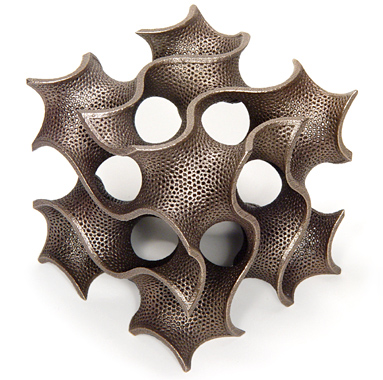
\includegraphics[max width=\linewidth]{../images/gyroid_hex.jpg}}\]

\begin{enumerate}
\def\labelenumi{\arabic{enumi})}
\setcounter{enumi}{4}
\tightlist
\item
  Bathsheba Grossman, Mathematical models,
  \texttt{http://www.bathsheba.com/math/}
\end{enumerate}

However, the great thing about the web is that lots of beautiful stuff
is free --- like these \emph{pictures} of the gyroid:
\[\href{http://www.bathsheba.com/math/gyroid/gyroid3q.jpg}{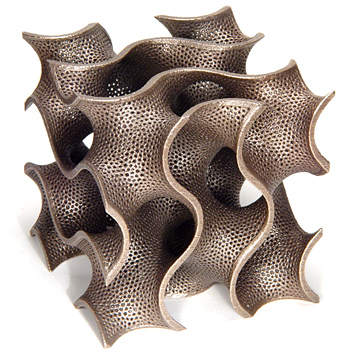
\includegraphics[max width=\linewidth]{../images/gyroid3q.jpg}}\]

I explained the 24-cell and 600-cell in
\protect\hyperlink{week155}{``Week 155''}. So, let me explain the gyroid
--- then I need to start cooking up a Christmas eve dinner!

A ``minimal surface'' is a surface in ordinary 3d space that can't
reduce its area by changing shape slightly. You can create a minimal
surface by building a wire frame and then creating a soap film on it. As
long as the soap film doesn't actually enclose any air, it will try to
minimize its area --- so it will end up being a minimal surface.

If you make a minimal surface this way, it will have edges along the
wire frame. A minimal surface without edges is called ``complete''. For
a long time, the only known complete minimal surfaces that didn't
intersect themselves were the plane, the catenoid, and the helicoid. You
get a ``catenoid'' by taking an infinitely long chain and letting it
hang to form a curve called a ``catenary''; then you use this curve to
form a surface of revolution, which is the catenoid:

\begin{enumerate}
\def\labelenumi{\arabic{enumi})}
\setcounter{enumi}{5}
\tightlist
\item
  Eric Weisstein, ``Catenoid'', from \emph{Mathworld},
  \texttt{http://mathworld.wolfram.com/Catenoid.html}
\end{enumerate}

In cylindrical coordinates the catenoid is given by the equation
\[r = c \cosh\left(\frac{z}{c}\right)\] for your favorite constant
\(c\).

A ``helicoid'' is like a spiral staircase; in cylindrical coordinates
it's given by the equation \[z = c\theta\] for some constant \(c\). You
can see a helicoid here --- and see how it can continuously deform into
a catenoid:

\begin{enumerate}
\def\labelenumi{\arabic{enumi})}
\setcounter{enumi}{6}
\tightlist
\item
  Eric Weisstein, ``Helicoid'', from \emph{Mathworld},
  \texttt{http://mathworld.wolfram.com/Helicoid.html}
\end{enumerate}

In 1987 a fellow named Hoffman discovered a bunch more complete
non-self-intersecting minimal surfaces with the help of a computer:

\begin{enumerate}
\def\labelenumi{\arabic{enumi})}
\setcounter{enumi}{7}
\tightlist
\item
  D. Hoffman, ``The computer-aided discovery of new embedded minimal
  surfaces'', \emph{Mathematical Intelligencer} \textbf{9} (1987),
  8--21.
\end{enumerate}

Since then people have gotten good at inventing minimal surfaces. You
can see a bunch here:

\begin{enumerate}
\def\labelenumi{\arabic{enumi})}
\setcounter{enumi}{8}
\item
  GRAPE (Graphics Programming Environment), ``Surface overview'',
  \texttt{http://www-sfb256.iam.uni-bonn.de/grape/EXAMPLES/AMANDUS/bmandus.html}
\item
  GANG (Geometry Analysis Numerics Graphics), ``Gallery of minimal
  surfaces'', \texttt{http://www.gang.umass.edu/gallery/min/}
\end{enumerate}

As you can see, people who work on mininal surfaces like goofy acronyms.
If you look at the pictures, you can also see that a minimal surface
needs to be locally saddle-shaped. More precisely, it has ``zero mean
curvature'': at any point, if it curves one way along one principal axis
of curvature, it has to curve an equal and opposite amount along the
perpendicular axis. Supposedly this was proved by Euler.

If we write this requirement as an equation, we get a second-order
nonlinear differential equation called ``Lagrange's equation'' --- a
special case of the Euler-Lagrange equation we get from any problem in
the variational calculus. So, finding new minimal surfaces amounts to
finding new solutions of this equation. Soap films solve this equation
automatically, but only with the help of a wire frame; it's a lot more
work to find minimal surfaces that are complete.

For the theoretical physicist, minimal surfaces also go by another name:
\emph{strings!} The ``worldsheet'' of a bosonic string is just a
2-dimensional surface in spacetime. The equation governing the string's
motion just says that the area of this surface can't be reduced by
wiggling it slightly. In other words, it's just Lagrange's equation.
There's a big difference between string theory and the theory of minimal
surfaces, though: in string theory we need to take quantum mechanics
into account! (Another big difference is that spacetime is a Lorentzian
rather than Riemannian manifold, unless we do a trick called ``Wick
rotation''.)

So, bosonic string theory is about the quantum version of soap films -
and ``D-branes'' serve as the wire frames. But if this reminds you of
``spin foams'', I should warn you: there are a few big differences. The
main thing is that spin foams are background-free: they don't live in
spacetime, they \emph{are} spacetime. So, it doesn't make any obvious
sense for them to minimize area, though Smolin has suggested it might
make an \emph{unobvious} kind of sense. All the fun must happen when the
``bubbles'' of a spin foam meet along their edges\ldots{} but we don't
really know how this should work, to create a foam with the right
consistency at large scales.

Anyway\ldots.

There are a lot of minimal surfaces that have periodic symmetry in 3
directions, like a crystal lattice. You can learn about them here:

\begin{enumerate}
\def\labelenumi{\arabic{enumi})}
\setcounter{enumi}{10}
\tightlist
\item
  Elke Koch, ``3-periodic minimal surfaces'',
  \texttt{http://staff-www.uni-marburg.de/\textasciitilde{}kochelke/minsurfs.htm}
\end{enumerate}

In fact, they have interesting relations to crystallography:

\begin{enumerate}
\def\labelenumi{\arabic{enumi})}
\setcounter{enumi}{11}
\tightlist
\item
  Elke Koch and Werner Fischer, ``Mathematical crystallography'',
  \texttt{http://www.staff.uni-marburg.de/\textasciitilde{}kochelke/mathcryst.htm\#minsurf}
\end{enumerate}

I guess people can figure out which of the 230 crystal symmetry groups
(or ``space groups'') can arise as symmetries of triply periodic minimal
surfaces, and use this to help classify these rascals. A cool mixture of
group theory and differential geometry! I don't get the impression that
they have completed the classification, though.

Anyway, Schoen's ``gyroid'' is one of these triply periodic minimal
surfaces. Schoen discovered it before the computer revolution kicked in.
He was working for NASA, and his idea was to use it for building
ultra-light, super-strong structures:

\begin{enumerate}
\def\labelenumi{\arabic{enumi})}
\setcounter{enumi}{12}
\tightlist
\item
  A. H. Schoen, ``Infinite periodic minimal surfaces without
  selfintersections'', \emph{NASA Tech. Note No.} \textbf{D-5541},
  Washington, DC, 1970.
\end{enumerate}

You can learn more about the gyroid here:

\begin{enumerate}
\def\labelenumi{\arabic{enumi})}
\setcounter{enumi}{13}
\tightlist
\item
  Eric Weisstein, ``Gyroid'', from \emph{Mathworld},
  \texttt{http://mathworld.wolfram.com/Gyroid.html}
\end{enumerate}

Apparently it's the only triply periodic non-self-intersecting minimal
surface with ``triple junctions''. I'm not quite sure what that means
mathematically, but I can see them in the picture!

I said that soap films weren't good at creating \emph{complete} minimal
surfaces. But actually, people have seen at least approximate gyroids in
nature, made from soap-like films:

\begin{enumerate}
\def\labelenumi{\arabic{enumi})}
\setcounter{enumi}{14}
\tightlist
\item
  P. Garstecki and R. Holyst, ``Scattering patterns of self-assembled
  gyroid cubic phases in amphiphilic systems'', \emph{J. Chem. Phys.}
  \textbf{115} (2001), 1095--1099.
\end{enumerate}

An ``amphiphilic'' molecule is one that's attracted by water at one end
and repelled by water at the other. For example, the stuff in soap.
Mixed with water and oil, such molecules form membranes, and really
complicated patterns can emerge, verging on the biological. Sometimes
the membranes make a gyroid pattern, with oil on one side and water on
other! It's a great example of how any sufficiently beautiful
mathematical pattern tends to show up in nature somewhere\ldots{} as
Plato hinted in his theory of ``forms''.

People have fun simulating these ``ternary amphiphilic fluids'' on
computers:

\begin{enumerate}
\def\labelenumi{\arabic{enumi})}
\setcounter{enumi}{15}
\item
  Nelido Gonzalez-Segredo and Peter V. Coveney, ``Coarsening dynamics of
  ternary amphiphilic fluids and the self-assembly of the gyroid and
  sponge mesophases: lattice-Boltzmann simulations'', available as
  \href{http://arxiv.org/abs/cond-mat/0311002}{\texttt{cond-mat/0311002}}.
\item
  Pittsburgh Supercomputing Center, ``Ketchup on the grid with
  joysticks'', \texttt{http://www.psc.edu/science/2004/teragyroid/}
\end{enumerate}

The second site above describes the ``TeraGyroid Project'', in which
people used 17 teraflops of computing power at 6 different facilities to
simulate the gyroidal phase of oil/water/amphiphile mixtures and study
how ``defects'' move around in what's otherwise a regular pattern. The
reference to ketchup comes from some supposed relationship between these
ternary amphiphilic fluids and how ketchup gets stuck in the bottle. I'm
not sure ketchup actually \emph{is} a ternary amphiphilic fluid, though!

Hmm. I just noticed a pattern to the websites I've been referring to:
first one about a ``Milky Way bar'', then one about a ``GRAPE'', and now
one about ketchup! I think it's time to cook that dinner.

\begin{center}\rule{0.5\linewidth}{0.5pt}\end{center}

\begin{quote}
\emph{Daydreaming admiring being\\
Quietly, open the world\\
I hear the time of the starry sky\\
Turning over at midnight}

--- Massive Attack
\end{quote}



\end{document}
